% Options for packages loaded elsewhere
\PassOptionsToPackage{unicode}{hyperref}
\PassOptionsToPackage{hyphens}{url}
%
\documentclass[
]{article}
\usepackage{lmodern}
\usepackage{amssymb,amsmath}
\usepackage{ifxetex,ifluatex}
\ifnum 0\ifxetex 1\fi\ifluatex 1\fi=0 % if pdftex
  \usepackage[T1]{fontenc}
  \usepackage[utf8]{inputenc}
  \usepackage{textcomp} % provide euro and other symbols
\else % if luatex or xetex
  \usepackage{unicode-math}
  \defaultfontfeatures{Scale=MatchLowercase}
  \defaultfontfeatures[\rmfamily]{Ligatures=TeX,Scale=1}
\fi
% Use upquote if available, for straight quotes in verbatim environments
\IfFileExists{upquote.sty}{\usepackage{upquote}}{}
\IfFileExists{microtype.sty}{% use microtype if available
  \usepackage[]{microtype}
  \UseMicrotypeSet[protrusion]{basicmath} % disable protrusion for tt fonts
}{}
\makeatletter
\@ifundefined{KOMAClassName}{% if non-KOMA class
  \IfFileExists{parskip.sty}{%
    \usepackage{parskip}
  }{% else
    \setlength{\parindent}{0pt}
    \setlength{\parskip}{6pt plus 2pt minus 1pt}}
}{% if KOMA class
  \KOMAoptions{parskip=half}}
\makeatother
\usepackage{xcolor}
\IfFileExists{xurl.sty}{\usepackage{xurl}}{} % add URL line breaks if available
\IfFileExists{bookmark.sty}{\usepackage{bookmark}}{\usepackage{hyperref}}
\hypersetup{
  pdftitle={用R玩转Spark------大规模数据分析和建模完全手册},
  pdfauthor={魏博},
  hidelinks,
  pdfcreator={LaTeX via pandoc}}
\urlstyle{same} % disable monospaced font for URLs
\usepackage[margin=1in]{geometry}
\usepackage{color}
\usepackage{fancyvrb}
\newcommand{\VerbBar}{|}
\newcommand{\VERB}{\Verb[commandchars=\\\{\}]}
\DefineVerbatimEnvironment{Highlighting}{Verbatim}{commandchars=\\\{\}}
% Add ',fontsize=\small' for more characters per line
\usepackage{framed}
\definecolor{shadecolor}{RGB}{248,248,248}
\newenvironment{Shaded}{\begin{snugshade}}{\end{snugshade}}
\newcommand{\AlertTok}[1]{\textcolor[rgb]{0.94,0.16,0.16}{#1}}
\newcommand{\AnnotationTok}[1]{\textcolor[rgb]{0.56,0.35,0.01}{\textbf{\textit{#1}}}}
\newcommand{\AttributeTok}[1]{\textcolor[rgb]{0.77,0.63,0.00}{#1}}
\newcommand{\BaseNTok}[1]{\textcolor[rgb]{0.00,0.00,0.81}{#1}}
\newcommand{\BuiltInTok}[1]{#1}
\newcommand{\CharTok}[1]{\textcolor[rgb]{0.31,0.60,0.02}{#1}}
\newcommand{\CommentTok}[1]{\textcolor[rgb]{0.56,0.35,0.01}{\textit{#1}}}
\newcommand{\CommentVarTok}[1]{\textcolor[rgb]{0.56,0.35,0.01}{\textbf{\textit{#1}}}}
\newcommand{\ConstantTok}[1]{\textcolor[rgb]{0.00,0.00,0.00}{#1}}
\newcommand{\ControlFlowTok}[1]{\textcolor[rgb]{0.13,0.29,0.53}{\textbf{#1}}}
\newcommand{\DataTypeTok}[1]{\textcolor[rgb]{0.13,0.29,0.53}{#1}}
\newcommand{\DecValTok}[1]{\textcolor[rgb]{0.00,0.00,0.81}{#1}}
\newcommand{\DocumentationTok}[1]{\textcolor[rgb]{0.56,0.35,0.01}{\textbf{\textit{#1}}}}
\newcommand{\ErrorTok}[1]{\textcolor[rgb]{0.64,0.00,0.00}{\textbf{#1}}}
\newcommand{\ExtensionTok}[1]{#1}
\newcommand{\FloatTok}[1]{\textcolor[rgb]{0.00,0.00,0.81}{#1}}
\newcommand{\FunctionTok}[1]{\textcolor[rgb]{0.00,0.00,0.00}{#1}}
\newcommand{\ImportTok}[1]{#1}
\newcommand{\InformationTok}[1]{\textcolor[rgb]{0.56,0.35,0.01}{\textbf{\textit{#1}}}}
\newcommand{\KeywordTok}[1]{\textcolor[rgb]{0.13,0.29,0.53}{\textbf{#1}}}
\newcommand{\NormalTok}[1]{#1}
\newcommand{\OperatorTok}[1]{\textcolor[rgb]{0.81,0.36,0.00}{\textbf{#1}}}
\newcommand{\OtherTok}[1]{\textcolor[rgb]{0.56,0.35,0.01}{#1}}
\newcommand{\PreprocessorTok}[1]{\textcolor[rgb]{0.56,0.35,0.01}{\textit{#1}}}
\newcommand{\RegionMarkerTok}[1]{#1}
\newcommand{\SpecialCharTok}[1]{\textcolor[rgb]{0.00,0.00,0.00}{#1}}
\newcommand{\SpecialStringTok}[1]{\textcolor[rgb]{0.31,0.60,0.02}{#1}}
\newcommand{\StringTok}[1]{\textcolor[rgb]{0.31,0.60,0.02}{#1}}
\newcommand{\VariableTok}[1]{\textcolor[rgb]{0.00,0.00,0.00}{#1}}
\newcommand{\VerbatimStringTok}[1]{\textcolor[rgb]{0.31,0.60,0.02}{#1}}
\newcommand{\WarningTok}[1]{\textcolor[rgb]{0.56,0.35,0.01}{\textbf{\textit{#1}}}}
\usepackage{longtable,booktabs}
% Correct order of tables after \paragraph or \subparagraph
\usepackage{etoolbox}
\makeatletter
\patchcmd\longtable{\par}{\if@noskipsec\mbox{}\fi\par}{}{}
\makeatother
% Allow footnotes in longtable head/foot
\IfFileExists{footnotehyper.sty}{\usepackage{footnotehyper}}{\usepackage{footnote}}
\makesavenoteenv{longtable}
\usepackage{graphicx,grffile}
\makeatletter
\def\maxwidth{\ifdim\Gin@nat@width>\linewidth\linewidth\else\Gin@nat@width\fi}
\def\maxheight{\ifdim\Gin@nat@height>\textheight\textheight\else\Gin@nat@height\fi}
\makeatother
% Scale images if necessary, so that they will not overflow the page
% margins by default, and it is still possible to overwrite the defaults
% using explicit options in \includegraphics[width, height, ...]{}
\setkeys{Gin}{width=\maxwidth,height=\maxheight,keepaspectratio}
% Set default figure placement to htbp
\makeatletter
\def\fps@figure{htbp}
\makeatother
\setlength{\emergencystretch}{3em} % prevent overfull lines
\providecommand{\tightlist}{%
  \setlength{\itemsep}{0pt}\setlength{\parskip}{0pt}}
\setcounter{secnumdepth}{-\maxdimen} % remove section numbering

\title{用R玩转Spark------大规模数据分析和建模完全手册}
\author{魏博}
\date{2020-01-07}

\begin{document}
\maketitle

{
\setcounter{tocdepth}{2}
\tableofcontents
}
\hypertarget{ux5e8f}{%
\section{序}\label{ux5e8f}}

Apache
Spark是一个基于可扩展性构建的分布式计算平台:Spark的api使来自多个数据源的输入变得很容易,并使用多种编程语言和算法来处理它以构建数据应用程序。R是数据科学和统计学中最强大的语言之一,因此将R与Spark连接起来非常有意义。幸运的是,R丰富的语言特性使得从R调用Spark的api看起来于在本地数据源上运行R类似。有了这两个系统的背景知识,你将能够在Spark中调用大量计算,或者从你最喜欢的R编程环境中并行运行R代码。
本书详细探讨了在R中使用Spark的方法,重点介绍了\texttt{sparklyr}包,它支持\texttt{dplyr}和R社区已知的其他包。它详细涵盖了所有的主要用例,从使用Spark引擎查询数据到探索性数据分析、机器学习、R代码的并行执行和流式处理。它还对运行Spark和监视作业执行进行了自洽的介绍。作者正是写这个话题的合适人员。Javier,Kevin和Edgar一直参与\texttt{sparklyr}开发项目。我很兴奋地看到他们把这本关于使用Spark和R的清晰而集中的指南组装得多么好。

我希望你喜欢这本书,并使用它来提你您的R工作量,并将它们与更广泛的Spark生态系统的功能连接起来。而且因为这里的所有基础模块都是开源的,所以可以毫不犹豫地向开发人员反馈如何改进这些工具。

--- Matei Zaharia 斯坦福大学助理教授,Databricks首先技术专家,Apache
Spark发明者

\begin{center}\rule{0.5\linewidth}{\linethickness}\end{center}

\hypertarget{ux524dux8a00}{%
\section{前言}\label{ux524dux8a00}}

在信息呈指数级增长的世界中,Apache
Spark等先进工具为解决我们今天面临的许多相关问题提供了支持。从基于数据驱动决策寻找改进方法的公司,到解决医疗、金融、教育和能源问题的研究机构,Spark比以往任何时候都能更快、更可靠地分析更多信息。

人们编写了各种各样的书籍来学习Apache Spark。例如,《Spark: The
Definitive Guide》是一个综合性的资源,《Learning
Spark》是一本介绍性的书籍,旨在帮助用户熟悉和运行Spark(两者都来自O'Reilly)。然而,在撰写本文时,既没有使用R计算语言学习Apache
Spark的书籍,也没有专门为R用户或潜在的R用户设计的书籍。

有一些在线资源可以学习R语言中的Apache
Spark。最著名的是Spark.rstudio.com网站和Spark.Apache.org上的Spark文档网站。这两个网站都是很好的在线资源;但是,上边的内容不打算让你从头到尾的阅读。它们都假设读者对Apache
Spark、R和集群计算有一定的了解。

这本书的目的是帮助所有人通过R使用Apache
Spark。另外,由于R编程语言是为了简化数据分析而创建的,我们也相信这本书可以为你提供学习用Spark解决数据分析问题的工具的最简单途径。第一章提供了一个介绍,帮助快速理解这些概念,并介绍了在自己的计算机上处理这些问题所需的工具。然后,我们会快速进入相关的数据科学主题、集群计算和高级主题。即使是最有经验的用户也会感兴趣。

因此,本书旨在成为一个对广大用户有用的资源,从渴望学习Apache
Spark初学者,到寻求理解为什么和如何通过R使用apachespark的有经验的读者。

本书结构如下:

\begin{itemize}
\tightlist
\item
  介绍 在前两章,第一章简介和第二章入门中,你将了解Apache
  Spark,R以及使用Spark和R执行数据分析的工具。
\item
  分析 在第3章分析中,你将学习如何使用R在Apache
  Spark中分析、探索、转换和可视化数据。
\item
  建模
  在第4章建模和第5章管道中,你将学习如何创建统计模型,以便在生产环境的工作流中提取信息、预测结果和自动化过程。
\item
  规模化
  到目前为止,这本书的重点是在你的个人电脑上执行操作和有限的数据格式。第6章集群,第7章连接,第8章数据,以及第9章调试,介绍了跨多台机器和数据格式执行分析和建模所需的分布式计算技术,以解决Apache
  Spark关注的大规模数据和计算问题。
\item
  扩展
  第10章扩展,描述了适用于特定相关用例的可选模块和扩展功能。拟将学习其他建模框架、图处理、用于深入学习的预处理数据、地理空间分析和大规模基因组学。
\item
  高级技术
  本书结尾是介绍一系列高级技术的章节,包括第11章分布式R,第12章流式计算,第13章社区贡献;这些内容是高级用户最感兴趣的。但是,当你学到本节时,其实并没有那么吓人;相反,这些章节将与前面的章节一样相关、有用和有趣。
\end{itemize}

第一组章节,1-5,简单地介绍了如何大规模执行数据科学和机器学习。如果你打算阅读这本书,同时也跟随代码示例,这些是考虑逐行执行代码的好章节。因为这些章节教你个人电脑涉及的所有概念。你不会利用多台电脑,而Spark却是为使用这些电脑而设计的。但别担心:下一章将详细介绍这一点!

第二组章节,6-9,介绍了使用Spark进行集群计算的令人激动的世界中的基本概念。事实上,他们还介绍了集群计算中一些不那么有趣的部分。但是相信我们,这些概念还是值得学习的。此外,每章中的概述部分都特别有趣、信息丰富、易于阅读,并有助于你直观地了解集群计算是如何工作的。对于这些章节,我们实际上并不建议逐行执行代码,尤其是在尝试从头到尾学习Spark的情况下。在拥有一个合适的Spark集群之后,你总是可以回过头来执行代码。但是,如果你已经有一个可以工作的集群,或者你真的很想得到一个集群,那么你可能需要使用第6章来选择一个集群,然后使用第7章来连接它。

第三组章节,10-13,展示了对大多数读者来说应该很有趣的工具,并且会使后续的操作更容易。这里有很多高级话题,一些主题自然比其他主题更感有意思;例如,你可能对分析地理数据集感兴趣,或者你对处理实时数据集更感兴趣,或者你希望两者兼得!基于个人兴趣或手头的问题,我们鼓励你执行与最相关的代码示例。这些章节中的所有代码都是为了在个人计算机上执行而编写的,但我们也鼓励你使用合适的Spark集群,因为你会拥有解决问题和优化大规模计算所需的工具。

\hypertarget{ux683cux5f0fux5316}{%
\subsection{格式化}\label{ux683cux5f0fux5316}}

代码生成的表用以下代码格式化:

\begin{Shaded}
\begin{Highlighting}[]
\CommentTok{# A tibble: 3 x 2}
\NormalTok{numbers text}
\OperatorTok{<}\NormalTok{dbl}\OperatorTok{>}\StringTok{ }\ErrorTok{<}\NormalTok{chr}\OperatorTok{>}
\DecValTok{1} \DecValTok{1}\NormalTok{ one}
\DecValTok{2} \DecValTok{2}\NormalTok{ two}
\DecValTok{3} \DecValTok{3}\NormalTok{ three}
\end{Highlighting}
\end{Shaded}

表的维度(行数和列数)在第一行中有描述,第二行是列名,第三行是列类型。我们在本书中使用的\texttt{tibble}包还提供了各种细微的视觉改进。

大多数绘图都使用\texttt{ggplot2}包和附录中提供的自定义主题进行渲染;但是,由于本书不关注数据可视化,因此我们只提供基本绘图的代码,其可能与应用的格式不匹配。如果你有兴趣学习R中更多关于可视化的知识,可以考虑专门的书籍,比如《R
Graphics Cookbook》(O'Reilly)。

\hypertarget{ux81f4ux8c22}{%
\subsection{致谢}\label{ux81f4ux8c22}}

感谢那些允许通过R使用Spark的程序包作者:Javier Luraschi、Kevin
Kuo、Kevin Ushey和JJ Allaire(\texttt{sparklyr});Romain
franois和Hadley Wickham(\texttt{dbplyr});Hadley Wickham和Edgar
Ruiz(\texttt{dpblyr});Kirill Mülller(\texttt{DBI});以及Apache
Spark项目本身的作者及其最初作者Matei Zaharia。

感谢为丰富Spark和R生态系统而发布扩展的程序包作者:Akhil
Nair(\texttt{crassy});Harry Zhu(\texttt{geospark});Kevin
Kuo(\texttt{graphframes}、\texttt{mleap}、\texttt{sparktf}和\texttt{sparkxgb});Jakub
Hava、Navdeep Gill、Erin LeDell和Michal
Malohlava(\texttt{rsparkling});Jan
Wijffels(\texttt{Spark.sas7bdat});Aki
Ariga(\texttt{sparkavro});Martin Studer(\texttt{sparkbq});Matt
Pollock(\texttt{sparklyr.nested});Nathan
Eastwood(\texttt{sparkts});Samuel Macêdo(\texttt{variantspark})。

感谢我们出色的编辑Melissa
Potter为我们提供指导、鼓励和无数小时的详细反馈,使这本书成为我们的著作中最好的一本。

感谢Bradley Boehmke,Bryan Adams,Bryan Jonas,Dusty Turner和Hossein
Falaki,感谢你们的技术评论、及时和坦率的反馈,并与我们分享专业知识。多亏了你们,许多读者才会有更愉快的阅读体验。

感谢RStudio、JJ Allaire和Tareef
Kawaf对这项工作的支持,感谢R的持续支持和鼓励。

Max
Kuhn,感谢你对第四章的宝贵反馈。在他的允许下,我们采用了他的精彩著作《特征工程与选择:预测模型的实用方法》(CRC出版社)中的例子。

我们也感谢所有间接参与但未在本节中明确列出的人们;我们真正站在了巨人的肩膀上。

这本书是用Yihui Xie的\texttt{bookdown},JJ Allaire和Yihui
Xie的\texttt{rmarkdown},Yihui Xie的\texttt{knitr}写成的;用Hadley
Wickham和Winston Chang的\texttt{ggplot2}完成可视化;用Daniel
Kallin和Javier Luraschi的\texttt{nomnoml}绘制图表;用John
MacFarlane的\texttt{pandoc}进行文档转换。

\hypertarget{ux884cux6587ux683cux5f0f}{%
\subsection{行文格式}\label{ux884cux6587ux683cux5f0f}}

本书使用下列排版风格:

\emph{斜体} 表示新的术语,URL,电子邮箱地址,文件名,和文件扩展名。

\texttt{固定宽度}
用于表示程序内容以及段落中引用的程序元素,如变量或函数名、数据库、数据类型、环境变量、语句和关键字。

\texttt{**重体固定宽度**} 展示用户输入的命令或其它文本。

\texttt{*斜体固定宽度*}
展示应该被用户提供的,或由上下文确定的值替换的文本。

\begin{quote}
用来表示注意事项或者建议。
\end{quote}

\begin{quote}
用来表示一般的注释。
\end{quote}

\hypertarget{ux4f7fux7528ux793aux4f8bux4ee3ux7801}{%
\subsection{使用示例代码}\label{ux4f7fux7528ux793aux4f8bux4ee3ux7801}}

补充材料(代码示例、练习等)可在https://github.com/r-spark/the-r-in-spark上下载。

这本书是来帮你完成工作的。一般情况下,如果本书提供了示例代码,你可以在你的程序和文档中使用。你不需要为了获得许可联系我们,除非你正在复制代码的重要部分。例如,编写一个使用本书中多段代码的程序不需要获得我们的许可。出售或分发O'Reilly书籍的示例光盘就需要获得许可。引用本书以及示例代码来回答问题也不需要许可。将本书中大量的示例代码合并到你的产品文档中就需要获得许可。

虽然我们会感谢你的引用,但是我们也不强制要求你这么做。引用通常包括标题、作者、出版商和ISBN。例如:``Mastering
Spark with R by Javier Luraschi, Kevin Kuo, and Edgar Ruiz (O'Reilly).
Copyright 2020 Javier Luraschi, Kevin Kuo, and Edgar Ruiz,
978-1-492-04637-0.''

如果你觉得你对代码示例的使用超出了合理使用或上述许可范围,\href{mailto:请通过permissions@oreilly.com与我们联系}{\nolinkurl{请通过permissions@oreilly.com与我们联系}}。

\hypertarget{ux7b2c1ux7ae0-ux5f15ux8a00}{%
\section{第1章 引言}\label{ux7b2c1ux7ae0-ux5f15ux8a00}}

\begin{quote}
你什么都不知道,Jon Snow。
\end{quote}

\begin{quote}
--- Ygritte
\end{quote}

随着信息以指数的速率增长,历史学家把这段历史时期称作信息时代也就不意外了。逐步加速的数据收集速度也创造了很多新的机会,并且必然会创造更多的机会。本章介绍一些用于解决大规模数据挑战的工具。首先,作为处理大规模数据集的流行工具,本章会介绍Apache
Spark。有了这一基础,我们会介绍R编程语言,它是专门设计用于简化数据分析的。最后,我们会介绍\texttt{sparklyr},该项目将R和Spark结合成为大家都可使用的强大工具。

\emph{第二章,这就开始}会介绍用于在个人电脑上执行Spark和R运算所需的预备知识,工具和步骤。你会学到如何安装和初始化Spark,了解常见操作,处理第一份数据和完成建模任务。本章的目的就是要帮助读者掌握处理大规模数据问题所需的概念和工具,而这些问题目前只有少数组织可以接触到。

然后,你可以继续学习如何分析大规模数据,以及构建模型支持预测趋势和发现隐藏在海量信息中的知识。接着,你可以掌握一些用于执行数据分析和大规模建模的工具。后续章节会帮助你从本地计算机中跳出来,转向计算集群,以便解决许多真实世界的问题。最后几章会介绍一些其他的话题,例如实时数据处理和图分析,可以帮助你真正的掌握任何规模数据分析的最先进的技能。本书的最后一章会介绍一些工具和想法,读者可以考虑在Spark和R社区中做些贡献。

我们希望,阅读本书能成为一种愉悦的经历,可以帮助你解决职业生涯的数据问题,并推动世界作出有利于所有人的更好决策。

\hypertarget{ux6982ux8ff0}{%
\subsection{概述}\label{ux6982ux8ff0}}

人类大约从公元前3000年苏美尔人时期就开始用美索不达米亚成熟的书写体系保存,获取,操作和沟通信息了
。根据使用的保存和处理技术,人类的信息处理可能分成四个不同的发展时期:前机械工具时期(公元前3000至公元后1450年),机械工具时期(1450--1840),电子机械时期(1840--1940),和电子时期(1940至今)\footnote{Laudon
  KC, Traver CG, Laudon JP (1996). ``Information technology and
  systems.'' Cambridge, MA: Course Technology。}。

数学家George
Stibitz在1942年使用词语digital来描述快速的电子脉冲\footnote{Ceruzzi PE
  (2012). Computing: a concise history. MIT Press.}。直到今天,我们把用电子格式存储的信息还叫做数字信息。相反,模拟信息表示用非电子格式存储的各种信息,例如手写笔记,书籍,报纸等。

世界银行发布的关于数字发展的报告给出了过去三十年保存下来的数字信息和模拟信息总量估计\footnote{Group
  WB (2016). The Data Revolution. World Bank Publications.}。这份报告指出数字信息大概在2003年超过了模拟信息,其总量有大约一千万太字节,大约相当于今天的一千万存储驱动。然而,这份报告中更相关的发现是,我们的数字信息正在以指数的速度增长。图1-1展示了这份报告的结论。注意到,每隔一年,世界上的信息都会增长10倍。

为了提供工具找出所有新的数字信息,许多公司都试图提供相关的功能,例如我们今天熟知的用于搜索网络的搜索引擎。给定海量的数字信息,管理如此规模的信息绝对是一项挑战。搜索引擎并不能存储所有的网页信息,支持在单一电脑上搜索网页。这就意味着它必须把信息分成几个文件,并存储在多个机器上。这项技术就是\emph{谷歌文件系统(Google
File System)},它在谷歌2003年发表的学术文献中有介绍\footnote{Ghemawat
  S, Gobioff H, Leung S (2003). ``The Google File System.'' In
  Proceedings of the Nineteenth ACM Symposium on Operating Systems
  Principles. ISBN 1-58113-757-5.}。

\begin{figure}
\centering
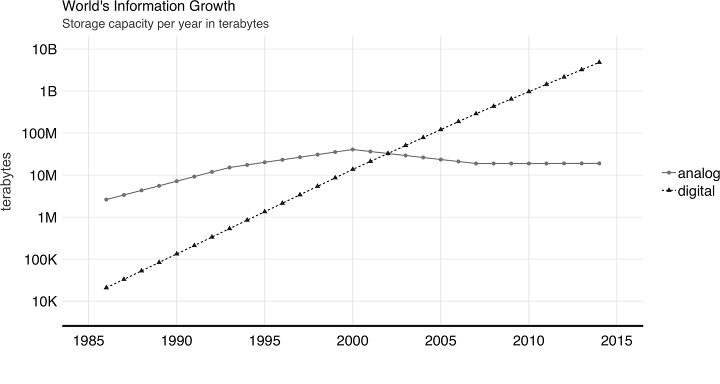
\includegraphics{figures/1_1.png}
\caption{图1-1. 全球存储信息能力}
\end{figure}

\hypertarget{hadoop}{%
\subsection{Hadoop}\label{hadoop}}

一年以后,谷歌发表了新的的文章,描述了如何在谷歌文件系统上执行操作,也就是后来的\emph{MapReduce}技术。\footnote{Dean
  J, Ghemawat S (2004). ``MapReduce: Simplified data processing on large
  clusters.'' In USENIX Symposium on Operating System Design and
  Implementation (OSDI).}。正如你可以预见到的,MapReduce中有两种操作:map和reduce。\emph{map}操作提供任意一种方法把每个文件转化为一个新的文件,而\emph{reduce}操作可以合并两个文件。两种操作都需要定制计算机代码,而MapReduce框架关注一次性在多个电脑上的自动执行。这两个操作足够支持网络上所有数据的处理,同时也提供足够的灵活性从数据中得到有意义的信息。

例如在图1-2中,我们可以使用MapReduce计算存放在不同机器上的两个不同文本文件的词语数量。map操作切分原始文件中的每个词语,并输出一个新的词语计数文件,其包含词语到计数的映射。reduce操作可以定义成对两个词语计数文件的合并,其通过整合每个词语的计数总数来实现。最终的文件会包含来自所有原始文件的词语计数。

词语计数通常是最基础的MapReduce示例,但是我们也可以使用MapReduce完成更加复杂和有趣的应用。例如,我们可以在谷歌的PageRank算法中对网页排序,该算法可以基于链接到一个网页的超链接数对所有网页排序,以及给出该网页的排位。

\begin{figure}
\centering
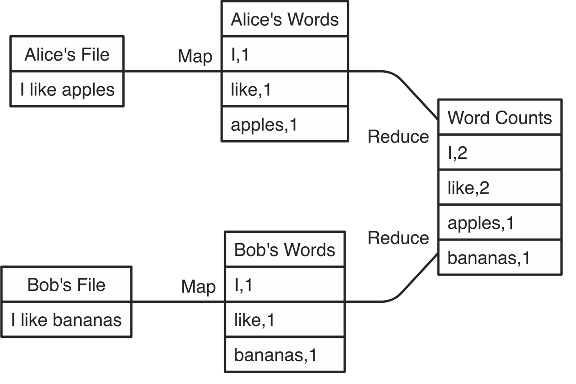
\includegraphics{figures/1_2.png}
\caption{图1-2. 跨多个文件的词语计数MapReduce作业示例}
\end{figure}

在谷歌发表了这些文献之后,雅虎的一个团队致力于实现谷歌文件系统和MapReduce作为一个单一的开源项目。这个项目就是2006发布的\emph{Hadoop},其中谷歌文件系统通过\emph{Hadoop分布式文件系统(Hadoop
Distributed File
System,HDFS)}。Hadoop项目使得基于分布式文件的计算可以被更多的用户和组织获取,这也使得MapReduce的能力突破了网络数据处理。

尽管Hadoop提供了在分布式文件系统上执行MapReduce操作的支持,但是它依然需要在每次数据分析的时候写好MapReduce操作代码。为了改进这一繁琐的过程,Facebook于2008年发布了Hive项目。它给Hadoop引入了\emph{结构化查询语句(Structured
Query
Language,SQL)}。这意味着大规模数据分析不再需要为每个MapReduce操作编写代码。相反,用户可以用SQL编写原生的,更加容易理解和编写的数据分析语句。

\hypertarget{spark}{%
\subsection{Spark}\label{spark}}

2009年,Apache
Spark开始作为加州大学伯克利分校AMP实验室的科研项目,以期改进MapReduce。Spark针对性的提供了更加丰富的MapReduce以外的运算符集合,便于优化多个机器上代码运行。Spark同时将数据加载到内存中,使得各种操作要比Hadoop的磁盘存储快很多。最新的一项结果显示,运行逻辑斯蒂回归,一种在第四章中介绍的数据建模技术,利用内存中数据集的Spark要比Hadoop快10倍\footnote{Zaharia
  M, Chowdhury M, Franklin MJ, Shenker S, Stoica I (2010). ``Spark:
  Cluster computing with working sets.'' HotCloud, 10(10-10), 95.}。类似于图1-3的结果在原始研究文献中也有展示。

\begin{figure}
\centering
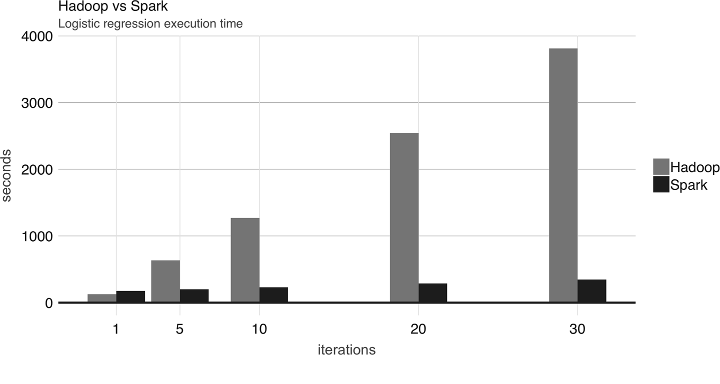
\includegraphics{figures/1_3.png}
\caption{图1-3. 逻辑回归在Hadoop和Spark上的性能}
\end{figure}

尽管Spark以内存操作性能而闻名,而当初设计时是作为支持内存和磁盘操作的一种通用执行引擎。例如,Spark创造了新的大规模排序记录,而这些数据并没有存在内存中。相反,Spark改进了网络序列化,网络改组,CPU缓存的高效利用,进而极大的提高了性能。如果你需要对大规模数据进行排序,世界上没有比Spark更快的系统了。

为了让你了解Spark有多快多高效,Hadoop使用了72分钟,2,100台计算机完成对100太字节数据的排序,但是Spark只用了23分钟和206台计算机。另外,Spark拥有云端排序记录,使得其成为云端对大规模数据进行排序的最剧性价比的解决方案。

\begin{longtable}[]{@{}lll@{}}
\toprule
& Hadoop记录 & Spark记录\tabularnewline
\midrule
\endhead
数据规模 & 102.5 TB & 100 TB\tabularnewline
使用时间 & 72分钟 & 23分钟\tabularnewline
节点数量 & 2,100 & 206\tabularnewline
核心数量 & 50,400 & 6,592\tabularnewline
磁盘 & 3,150 GB/秒 & 618 GB/秒\tabularnewline
网络 & 10 GB/秒 & 10 GB/秒\tabularnewline
排序速度 & 1.42 TB/分钟 & 4.27 TB/分钟\tabularnewline
排序速度/节点 & 0.67 GB/分钟 & 20.7 GB/分钟\tabularnewline
\bottomrule
\end{longtable}

Spark也比Hadoop易用。例如,词语计数的MapReduce示例在Hadoop中需要50行代码,而在Spark中只需要2行代码。正如所见,和Hadoop相比,Spark更快,更高效,更易用。

2010年,Spark作为开源项目发布出来,并于2013年捐赠给了Apache软件基金会。Spark执行Apache
2.0协议,运行用户免费使用,修改和分发。Spark有超过1,000名贡献者,是Apache软件基金会中最活跃的项目。

下面的表述介绍了Spark的定位。我们可以按照项目网站那样正式介绍Apache
Spark:

\begin{quote}
Apache Spark是一个面向大规模数据处理的统一分析引擎。
\end{quote}

为了帮助我们理解Apache Spark的概念,我们把它分成如下几个方面:

\begin{itemize}
\item
  统一

  Spark支持许多程序包,集群技术和存储系统。
\item
  分析

  分析是发现和理解数据,以期产出和沟通信息的行为。
\item
  引擎

  Spark是高效的和原生的。
\item
  大规模

  你可以把大规模理解成集群规模,一些连接一起的,共同工作的计算机。
\end{itemize}

Spark可以看做是一种\emph{引擎},因为它是原生和高效的。它的原生性是因为Spark可以优化和执行原生代码,也就是说,对于Spark中的程序代码并没有什么类型限制。它的高效性是因为Spark可以有效利用内存,网络和CPU加速计算集群中的数据处理算法,正如之前提到的,比其它技术都要快速。

这些特点使得Spark在许多分析任务中,例如Netflix的电影排序,蛋白质序列对齐,和CERN的高能物理分析,成为理想的工具。

作为一种\emph{统一}的平台,Spark可以支持许多集群技术和多种数据源。你可以分别在第六章和第八章中了解到。它也可以支持许多不同的程序包,例如Spark
SQL,MLlib,GraphX和Spark
Streaming,分别支持分析,建模,图处理和实时数据处理。总之,Spark是一种支持请求集群,数据源和各种程序包的平台,进而实现大规模计算,如图1-4所示。

\begin{figure}
\centering
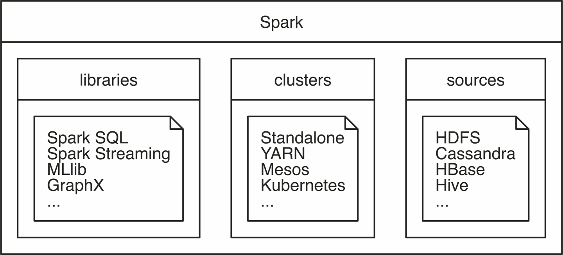
\includegraphics{figures/1_4.png}
\caption{图1-4. Spark,面向大规模数据处理的统一分析引擎}
\end{figure}

Spark支持大规模运算,意味着Spark的良好用例应该是使用多台机器解决问题。例如,当数据无法在单个磁盘或内存中存放,Spark会是一种良好的备选方案。然而,你也可以在面对非大规模问题的时候考虑使用Spark。此时,多台计算机可以加速计算。例如,CPU密集型的模型和科学模拟也可以从Spark中受益。

因此,Spark不但擅长解决大规模数据处理问题,即通常所说的\emph{大数据}(数据集比传统的要更加庞大和复杂),而且擅长解决大规模计算问题,即通常所说的\emph{大计算}(协调使用大量CPU和内存资源的工具和技术)。大数据经常需要大计算,但是\emph{大计算不一定需要大数据}。

大数据和大计算问题通常很容易识别。如果数据不能存放在单个机器,你就遇到了大数据问题;如果数据可以存放在单个机器,但是数据处理却需要数天,数周甚至更长的时间来完成,你就遇到了大计算问题。

但是,还有第三类问题,既不是大数据问题,也不是大计算问题,它们也可以从类似Spark的集群计算框架中受益良多。这类问题,有以下几种场景:

\begin{itemize}
\item
  高速性

  假设你有一个10GB的数据集,它的数据处理过程需要30分钟。这既不是一个大数据问题也不是一个大计算问题。但是,如果你突然要想着改进模型的准确率,减少运行时间到3分钟以内,这就是一个显著的改进。这种数据分析速度的改进可以带来有意义的推进和生产力的提高。另外,你也可能需要更快的处理数据速度,比如支持股票交易。尽管三分钟已经足够快,但是这对于实时数据处理依然很慢。这种场景下,你可能需要在几秒内甚至几毫秒内完成数据处理。
\item
  多样性

  你可能有了一个高效的数据收集流程,从多个数据源收集数据放在一个位置,通常是一个数据库。这个过程可能已经非常高效并且接近实时。这样的过程就是通常所说的\emph{抽取,转换和加载}(Extract,
  Transform,
  Load,ETL);数据从多个数据源抽取,转换成所需的格式,加载到单个数据存储结构中。尽管这一方法已经流行了多年,但是其中的权衡是添加新的数据源代价很高。因为系统是集中控制的,并且是严密操作的,任何改变都可能使整个过程暂停;因此,添加新的数据源通常要花费很长的时间才能实现。相反,你可以把全部数据按照自然格式存放,并且按照需要使用集群处理,即数据湖的架构。另外,按照原始格式存放数据支持处理图片,声音,和视频格式的新文件,而不需要明确如何把它们放进传统的结构化存储系统。
\item
  真实性

  当使用多个数据源的时候,你可能发现它们之间的数据质量参差不齐,需要专门的分析方法来改进准确性。例如,假设你有一个城市列表,取值包括旧金山,西雅图,和波士顿。当数据包含拼错的单词,例如``Bston'',会发生什么呢?在传统的关系型数据库中,这类非法输入可能会被舍弃。但是,舍弃取值并不一定所以情形下是最好的方法;你会希望利用地理编码,交叉验证数据源,或者尽最大努力匹配来纠正这些字段。所以,理解和改进原始数据源的真实性可以带来更准确的结果。
\end{itemize}

如果我们把``海量性''当做是大数据的同义词,你就得到了方便记忆的大数据的4个V。一些人也把它扩展成5个V甚至10个V。除了几个便于记忆的符号,今天集群计算也正在以更加创新的方式使用。看到各个组织实验新的工作流,以及传统意义上并不适用集群计算的各种任务,已经不再稀奇。更多的源于大数据的热潮都是这类问题。严格意义上讲,你不是在解决大数据,但是依然可以从大数据和大计算工具的使用中获益。

我们希望本书可以帮助你理解集群计算的机遇和局限,特别是使用Apache
Spark和R的机遇和局限。

\hypertarget{r}{%
\subsection{R}\label{r}}

R编程语言源于诞生在贝尔实验室的S语言。Rick
Becker在2016年的useR会议上解释,在那时的贝尔实验室里,计算是通过调用Fortran语句写成的子程序而实现的,而这种程序显然不好处理。而S计算语言当时是作为一种接口语言而设计的,它可以解决特殊的问题,而不需要使用其他语言,例如Fortran。S语言的发明者,John
Chambers在图1-5中给出了S是如何设计出来了,进而提供简化数据处理的一种接口,他的共同发明者也在2016年的useR!上展示了这一原图,启发了S的设计。

\begin{figure}
\centering
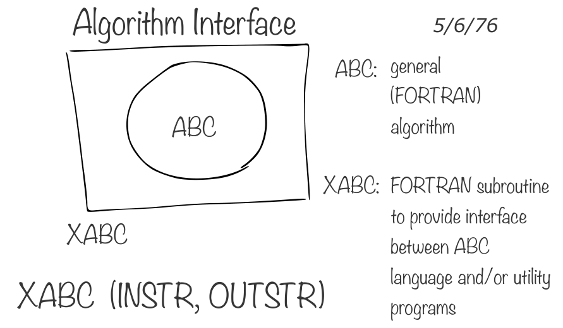
\includegraphics{figures/1_5.png}
\caption{图1-5. John Chambers的接口语言图 (Rick Becker useR 2016)}
\end{figure}

R语言是S语言一种现代而自由的实现。特别的,根据《面向统计计算的R项目》:

\begin{quote}
R是一种面向统计计算和图形学的编程语言和免费软件。
\end{quote}

处理数据的时候,我们相信R语言有两大特点:

\begin{itemize}
\item
  R语言

  R是由统计学家设计的,也是面向统计学家使用的。这意味着R是少有的,成功的面向非编程人员的编程语言之一。所以学习R会更加自然。另外,因为R语言是其他语言和工具的接口,所以R可以让你更多的关注理解问题,而更少的花在计算机科学和工程上。
\item
  R社区

  R社区通过\emph{R语言综合文档网络(Comprehensive R Archive
  Network,CRAN)}提供了丰富的程序包,支持安装即时可用的程序包,来执行各种任务------最享有盛名的高质量数据操作,可视化,和统计模型。许多操作只能在R中进行。另外,R社区是一个热情的,活跃的组织,这些优秀的朋友都愿意帮助你成功。R社区提供的许多程序包,到目前为止,都是统计计算的最优选择。一些下载最多的程序包包括:操作数据的\texttt{dplyr},分析聚类的\texttt{cluster},可视化数据的\texttt{ggplot2}。通过画出每天CRAN里R程序包的下载量,图1-6定量刻画了R社区的增长。
\end{itemize}

\begin{figure}
\centering
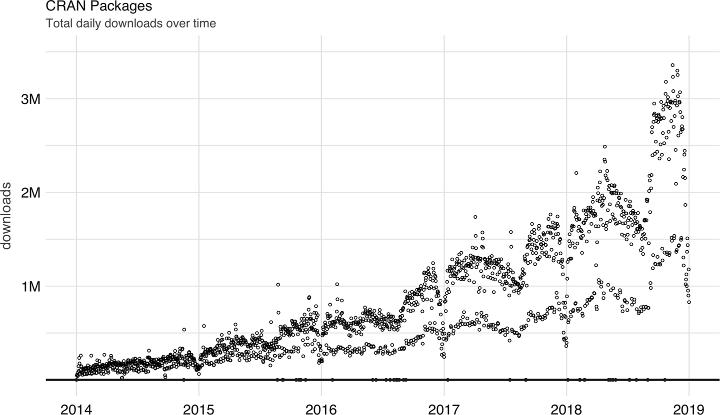
\includegraphics{figures/1_6.png}
\caption{图1-6. CRAN程序包每日下载量}
\end{figure}

除了统计分析,R也用在其他领域。以下领域和本书高度相关:

\begin{itemize}
\item
  数据科学

  数据科学基于来自统计学和计算机科学的知识和实践,通过数据分析和建模技术把原始数据变成深刻理解\footnote{Wickham
    H, Grolemund G (2016). R for data science: import, tidy, transform,
    visualize, and model data. O'Reilly Media, Inc}。统计学的方法提供了理解世界和进行预测的坚实基础,而计算机模型中的自动化技术可以让我们简化统计分析并易于实现。一些人认为,统计学应该重新命名为数据科学\footnote{Wu
    CJ (1997). ``Statistics = Data Science?''},然而数据科学结合了计算机的进展,并超出了统计学的范畴\footnote{Cleveland
    WS (2001). ``Data Science: An Action Plan for Expanding the
    Technical Areas of the Field of Statistics?''}。本书给出了统计学中常见的分析和建模技术,但是会应用到大数据集上,而这又需要分布式计算的成果。
\end{itemize}

\begin{itemize}
\item
  机器学习

  机器学习利用来自于统计学和计算机科学的实践。但是,它更多的关注自动化和预测。例如,Arthur
  Samuel在实现跳棋的计算机自动化程序的时候发明了词语machine
  learning\footnote{Samuel AL (1959). ``Some studies in machine learning
    using the game of checkers.'' IBM Journal of research and
    development, 3(3), 210--229.}。尽管我们可以在专门的游戏上实践数据科学,但是编写一个跳棋的程序需要我们自动化整个过程。因此,这个问题就是机器学习的范畴,而不是数据科学的范畴。机器学习使得许多用户在无意识中利用统计学的方法成为可能。机器学习中最重要的一个应用是过滤垃圾邮件。在这个例子中,只做数据分析和对每个邮箱账户建模是不可行的,因此机器学习可以自动化发现垃圾邮件的整个过程,并在用户没有参与的情况下过滤出去。本书给出了把数据科学工作流转换为完全自动化的机器学习的方法,例如,支持构建和导出Spark流程,以便容易的在自动化环境中复用此流程。
\end{itemize}

\begin{itemize}
\item
  深度学习

  深度学习建立在统计学,数据科学和机器学习知识的基础上,并受到生物神经系统的些许启发而定义模型。当梯度散失问题通过一次一层的训练解决后,深度学习就从神经网络模型逐步进化了\footnote{Hinton
    GE, Osindero S, Teh Y (2006). ``A fast learning algorithm for deep
    belief nets.'' Neural computation, 18(7), 1527--1554.},并被证明在图像识别和语音识别任务中非常强大。例如,在语音助手应用中,诸如Siri,Alexa,Cortana,或谷歌助手,实现语音到文本转换的模型大部分都是基于深度学习模型。尽管\emph{图形处理器(Graphic
  Processing Units,GPUs)}已经成功的用在了训练深度学习过程中\footnote{Krizhevsky
    A, Sutskever I, Hinton GE (2012). ``Imagenet classification with
    deep convolutional neural networks.'' In Advances in neural
    information processing systems, 1097--1105.},一些数据集并不能在单个GPU上处理。另一个事实是,深度学习模型需要大量的数据。这也需要在多个机器上预处理一下,然后才交给单个GPU训练。本书并不会直接给出深度学习模型的任何参考文献。但是你可以使用我们在本书中给出的方法,准备深度学习数据。在未来几年里,使用深度学习大规模计算技术会变得非常普遍。事实上,Spark的最新版本已经加入了为执行深度学习训练而优化过的模型。
\end{itemize}

处理上述几个领域时,你要么会面对逐渐增大的数据集,要么会面对逐渐复杂的计算过程。这些流程执行起来都很慢,或者某些时候在单台计算机上变得不可能。但是,要知道,Spark并不一定是所有计算问题的答案。而面对R中的计算问题时,使用以下技术会很有效:

\begin{itemize}
\item
  采样

  第一个要尝试的技术是通过采样,减少需要处理的数据量。然而,我们必须使用可靠的统计学原理,合适地采样数据。例如,选取有序数据集的头部数据是不够的。使用随机采样,会得到占比较少的数据集。这些都可以通过分层采样克服,但是选取合适的类别增加了算法复杂度。讲解如何进行合适的统计采样超出了本书的范畴,但是有很多有用的资源都是关于这个话题的。
\item
  分析器

  你可以试着理解为什么计算很慢,进而需要改进。分析器是检查代码执行情况,帮助识别瓶颈的工具。在R中,R的分析器,\texttt{profvis}程序包和RStudio的分析器功能可以让你轻松的重试和可视化一个分析器。然而,优化代码通常并不容易。
\item
  纵向扩展

  加速计算通过可以通过购买更快或者更强劲的硬件(即提高机器内存,更新硬盘,或者使用CPU更多的计算器)来实现。这些手段叫做纵向扩展。但是,对于单个计算机的纵向扩展通常存在硬极限,即使使用大量的CPU,你还需要新的框架来有效地并行化计算。
\item
  横向扩展

  最后,我们可以考虑把计算和存储扩大到对台机器上。这种手段提供了最高纬度的扩展性能。因为你可以使用任意数量的机器来执行计算。这个技术通常叫做横向扩展。但是,有效的扩展计算是一项复杂的实践,特别是没有使用专门的工具和框架,例如Apache
  Spark的时候。
\end{itemize}

最后一点更加具体的介绍了本书的目的,即Apache
Spark提供的分布式计算系统的能力,借助R解决数据科学和相关领域中有意义的计算问题。

\hypertarget{sparklyr}{%
\subsection{\texorpdfstring{\texttt{sparklyr}}{sparklyr}}\label{sparklyr}}

考虑到Spark提供的计算能力和R语言的易用性,我们很自然的想让二者无缝的结合起来。这也是R社区期望的:提供Spark接口的R程序包用起来很简单,并与其它R程序包兼容,而且可以在CRAN上找到。为此,我们开始开发\texttt{sparklyr}。第一版,\texttt{sparklyr\ 0.4},在2016年的useR!大会上发布。第一版包括对\texttt{dplyr},\texttt{DBI},建模工具\texttt{MLlib}的支持,以及支持类似H2O的\texttt{rsparkling}程序包的可扩展API。
从此,许多新的功能和改进在\texttt{sparklyr\ 0.5,\ 0.6,\ 0.7,\ 0.8,\ 0.9}和\texttt{1.0}做了实现。

根据官方定义,\texttt{sparklyr}是Apache
Spark的R语言接口。它可以通过CRAN获取,像其他CRAN程序包一样工作。这意味着人们无需知道Spark的版本,易于安装,同时服务于R社区,兼容其他R程序包,并接受来自R社区的使用反馈,等等。它托管在GitHub,遵循Apache
2.0协议,允许克隆,修改,并参与项目开发。使用\texttt{sparklyr}的用户应该包含以下角色:

\begin{itemize}
\item
  新用户

  对于新用户,我们坚信\texttt{sparklyr}提供了使用Spark的最简单的方式。我们希望本书的前面几章可以帮助你逐渐熟悉并毫无压力的使用Spark,进而为长期任务做准备。
\item
  数据科学家

  对于已经使用和钟爱R的数据科学家,\texttt{sparklyr}整合了许多其他的R实践和程序包,例如\texttt{dplyr},\texttt{magrittr},\texttt{broom},\texttt{DBI},\texttt{tibble},\texttt{rlang},以及其它框架,让你使用Spark从容自如。而对于R和Spark的新手,\texttt{sparklyr}的高级别工作流整合和低级别扩展机制保证Spark是一个高产的环境,可以满足每个数据科学家的需求和技能。
\item
  专家用户

  对于已经深度使用Spark,并可以编写Scala原生代码的用户,可以考虑让你的Spark程序包作为一个R程序包贡献给R社区。一个多样的,强大的社区可以让你的工作贡献出最好的价值,促进开源社会的发展。
\end{itemize}

我们编写这本书是为了介绍和传授Apache
Spark和R融合的部分。\texttt{sparklyr}就是把这些社区,期望和未来方向,程序包及其扩展整合在一起的R程序包。我们相信,有机会使用这本书来搭起R和Spark社区的桥梁:给R社区介绍为什么Spark让人兴奋,给Spark社区介绍为什么R如此伟大。两个社区都在使用不同的技术和背景来解决相似的问题。因此,我们希望\texttt{sparklyr}可以是创新的肥沃土壤,是新手的好客之地,是数据科学达人的高产环境,也是集群计算,数据科学,机器学习一起交流的开放社区。

\hypertarget{ux5c0fux7ed3}{%
\subsection{小结}\label{ux5c0fux7ed3}}

本章介绍了Spark这一现代而强大的计算平台,R这一易用的,基于扎实的统计建模理论的计算语言,以及\texttt{sparklyr}这一连接两个技术和社区的项目。w我们处在一个信息指数级增长的世界,学习如何分析大规模数据可以帮助你解决当今人类面临的问题和机遇。但是,在分析数据之前,第二章会介绍本书后面内容所需的工具。确保你可以明白每一步操作,并花点时间安装推荐的工具,它们会成为你经常使用和喜爱的资源。

\begin{center}\rule{0.5\linewidth}{\linethickness}\end{center}

\hypertarget{ux7b2c2ux7ae0-ux5f00ux59cb}{%
\section{第2章 开始}\label{ux7b2c2ux7ae0-ux5f00ux59cb}}

\begin{quote}
I always wanted to be a wizard.
\end{quote}

\begin{quote}
--- Samwell Tarly
\end{quote}

完成第一章的学习,你应该熟悉了Spark可以解决的各类问题。显而易见,Spark利用多台计算机来解决数据无法在单个机器上运行或者计算太慢的问题。如果你是R的新手,也可以看到,把Spark和数据科学工具,例如可视化工具\texttt{ggplot2},数据变换的\texttt{dplyr},结合起来可以给大规模数据科学项目带来美好的愿景。我们也希望你为自己成为大规模数据计算高手而感到兴奋。

在本章中,我们会浏览一下成为Spark高手所需要的工具。我们鼓励你能够实现本章的代码,因为这样会让你理解分析,建模,读取和写入数据的各种动作。换句话说,你需要坚持不懈,在使用Spark前反复实践。

在第三章中,我们会深入介绍分析,建模,并给出在单个集群上,也就是你的个人电脑上运行的例子。后续章节介绍集群计算,以及成功在多台机器上运行代码所需的概念和技术。

\hypertarget{ux6982ux8ff0-1}{%
\subsection{概述}\label{ux6982ux8ff0-1}}

R使用\texttt{sparklyr}来打通Spark和本地集群,整个过程和安装加载\texttt{sparklyr}程序包一样简单,后面安装Spark也通过\texttt{sparklyr}完成。但是,我们假设你在使用一个全新的电脑运行Windows,macOS或者Linux,因此我们会在连接本地Spark集群前,完成预备操作。

尽管本章是为了在个人电脑上使用Spark做准备,一些读者可能已经有了Spark集群,或者喜欢使用在线Spark集群。例如,Databricks托管了一个免费的社区版的Spark,你可以很容易的从浏览器访问。如果你最终选择了这条路,可以跳过``预备操作''。但是要确保你查阅了合适的资源,支持已有的或在线的Spark集群。或者,完成预备操作后,你首先要学习如何连接Spark。我们会介绍本书后续章节中用到的最重要的工具和操作。我们不会过多关注教授概念或者如何使用概念。我们不可能在一章中解释完建模或流式计算。但是,完成本章的学习让你窥见到Spark的能力,以及确信工具已经完成正确的部署,可以应付未来更多棘手的问题了。

所用的工具大部分都分成R代码和Spark网络接口。所有Spark操作都在R中运行。但是,分布式操作的监控动作在Spark的网络接口操作,你可以从任何一个网络浏览器加载看到。然后我们断开本地集群的连接。虽然容易忘记,我们还是强烈建议在使用本地集群和共享集群的时候能够记得这一操作.

本章末尾会介绍一些功能,使得在Rstudio中操作Spark更容易。更具体的,我们会介绍由\texttt{sparklyr}实现的RStudio扩展。但是,如果你喜欢使用Jupyter
Notebooks或者你的集群已经装好了别的R用户界面,确保你可以通过纯R代码使用Spark。现在,让我们开始学习预备操作。

\hypertarget{ux9884ux5907ux64cdux4f5c}{%
\subsection{预备操作}\label{ux9884ux5907ux64cdux4f5c}}

R可以在许多平台和环境中运行。所以,不管你用Windows,Mac,还是Linux,第一步都需要从r-project.org安装R。具体信息在``安装R''中有说明。

大部分人在使用编程语言时会使用工具,以便让编程更加高效。对于R,RStudio就是这样一个工具。严格地说,RStudio是一个\emph{集成开发环境(integrated
development
environment,IDE)},现在它也支持许多平台和环境。如果还没有安装Rstudio,我们强烈推荐你安装,具体操作见``安装RStudio''。

\begin{quote}
使用Windows的时候,我们建议不要使用路径上有空格的目录。如果运行\texttt{getwd()}返回了带有空格的路径,可以使用\texttt{setwd("path")}换成不带空格的路径,或者把RStudio项目创建到没有空格的路径中。
\end{quote}

另外,因为Spark是用Scala实现的,运行在Java虚拟机(Java Virtual
Machine,JVM)上,所有你还需要给系统安装Java
8。你的系统可能装了Java,但是还需要检查版本,按照``安装Java''的内容升级或降级。你可以使用如下R命令检查安装在系统的版本:

\begin{verbatim}
system("java -version")
java version "1.8.0_201"
Java(TM) SE Runtime Environment (build 1.8.0_201-b09)
Java HotSpot(TM) 64-Bit Server VM (build 25.201-b09, mixed mode)
\end{verbatim}

你也可以运行\texttt{Sys.setenv(JAVA\_HOME\ =\ "path-to-java-8")},使用\texttt{JAVA\_HOME}环境变量来指定具体的Java版本,或者,在安装\texttt{sparklyr}之前,确保R环境可以使用Java
8版本。

\hypertarget{ux5b89ux88c5sparklyr}{%
\subsubsection{\texorpdfstring{安装\texttt{sparklyr}}{安装sparklyr}}\label{ux5b89ux88c5sparklyr}}

和许多其他的R程序包一样,你可以使用如下命令安装CRAN上的\texttt{sparklyr}:

\begin{Shaded}
\begin{Highlighting}[]
\KeywordTok{install.packages}\NormalTok{(}\StringTok{"sparklyr"}\NormalTok{)}
\end{Highlighting}
\end{Shaded}

本书的示例假设你使用最新版本的\texttt{sparklyr}。你可以运行如下代码,验证你的版本是不是我们的一样新:

\begin{Shaded}
\begin{Highlighting}[]
\KeywordTok{packageVersion}\NormalTok{(}\StringTok{"sparklyr"}\NormalTok{)}
\NormalTok{[}\DecValTok{1}\NormalTok{] }\StringTok{'1.0.2'}
\end{Highlighting}
\end{Shaded}

\hypertarget{ux5b89ux88c5spark}{%
\subsubsection{安装Spark}\label{ux5b89ux88c5spark}}

使用\texttt{sparklyr}安装:

\begin{Shaded}
\begin{Highlighting}[]
\KeywordTok{library}\NormalTok{(sparklyr)}
\end{Highlighting}
\end{Shaded}

这个代码可以实现R中所有的\texttt{sparklyr}函数,非常有用。否则,你需要带着前缀\texttt{sparklyr::}运行每一个\texttt{sparklyr}命令。

你可以简单的通过运行\texttt{spark\_install()}安装Spark。这个命令可以在本地电脑上下载,安装和配置最新版本的Spark。但是,因为我们这本书是根据Spark
2.3编写的,所以你也可以安装这个版本,并顺畅的运行所有示例:

\begin{Shaded}
\begin{Highlighting}[]
\KeywordTok{spark_install}\NormalTok{(}\StringTok{"2.3"}\NormalTok{)}
\end{Highlighting}
\end{Shaded}

你可以运行如下命令,输出所有可以安装的Spark版本:

\begin{Shaded}
\begin{Highlighting}[]
\KeywordTok{spark_available_versions}\NormalTok{()}
\CommentTok{## spark 1 1.6 2 2.0 3 2.1 4 2.2 5 2.3 6 2.4}
\end{Highlighting}
\end{Shaded}

你可以使用Spark版本信息安装特定的版本,或者也可以明确Hadoop版本。例如,要安装Spark
1.6.3,你可以运行:

\begin{Shaded}
\begin{Highlighting}[]
\KeywordTok{spark_install}\NormalTok{(}\DataTypeTok{version =} \StringTok{"1.6.3"}\NormalTok{)}
\end{Highlighting}
\end{Shaded}

你也可以使用如下命令,检查已经安装的版本:

\begin{Shaded}
\begin{Highlighting}[]
\KeywordTok{spark_installed_versions}\NormalTok{()}
\NormalTok{spark hadoop dir}
\DecValTok{7} \DecValTok{2}\NormalTok{.}\FloatTok{3.1} \FloatTok{2.7} \OperatorTok{/}\NormalTok{spark}\OperatorTok{/}\NormalTok{spark}\DecValTok{-2}\NormalTok{.}\FloatTok{3.1}\OperatorTok{-}\NormalTok{bin}\OperatorTok{-}\NormalTok{hadoop2}\FloatTok{.7}
\end{Highlighting}
\end{Shaded}

Spark的安装路径通常是Spark的主目录,可以通过R代码和系统配置的\texttt{SPARK\_HOME}标识符来定义。当你使用安装有\texttt{sparklyr}的本地Spark集群时,这个路径是已知的,不需要额外的配置。

最后,要卸载具体版本的Spark,你可以指定Spark和Hadoop的版本信息,运行\texttt{spark\_uninstall()},如下:

\begin{Shaded}
\begin{Highlighting}[]
\KeywordTok{spark_uninstall}\NormalTok{(}\DataTypeTok{version =} \StringTok{"1.6.3"}\NormalTok{, }\DataTypeTok{hadoop =} \StringTok{"2.6"}\NormalTok{)}
\end{Highlighting}
\end{Shaded}

\begin{quote}
默认的安装路径是:macOS和Linux的\textasciitilde/spark,Windows的\%LOCALAPPDATA\%/spark。要定制化安装路径,可以在\texttt{spark\_install()}和\texttt{spark\_connect()}之前运行\texttt{options(spark.install.dir\ =\ "installation-path")}。
\end{quote}

\hypertarget{ux8fdeux63a5}{%
\subsection{连接}\label{ux8fdeux63a5}}

到目前为止,我们只安装了本地集群。本地集群对于初始学习,测试代码,轻松的排查故障非常有好处。后面的章节会介绍在哪里发现,安装和连接真正的有多台机器的Spark集群。但是对于开始的几章,我们只会使用本地集群。

要连接本地集群,只需运行如下代码:

\begin{Shaded}
\begin{Highlighting}[]
\KeywordTok{library}\NormalTok{(sparklyr)}
\NormalTok{sc <-}\StringTok{ }\KeywordTok{spark_connect}\NormalTok{(}\DataTypeTok{master =} \StringTok{"local"}\NormalTok{, }\DataTypeTok{version =} \StringTok{"2.3"}\NormalTok{)}
\end{Highlighting}
\end{Shaded}

\begin{quote}
如果你使用的是自己的或者在线的Spark集群,确保你是按照集群管理员的配置或者在线文档进行连接。如果你需要指针,可以参考第七章,它会详细介绍如何连接Spark集群。
\end{quote}

\texttt{master}参数明确了Spark集群中哪一个是主机器。这个机器通常叫做\emph{驱动节点(driver
node)}。使用多台机器的真实集群时,你会发现大部分机器是工作机器,一个是主机器。因为我们只有一个单台机器的本地集群,从现在开始我们会默认使用``\texttt{local}''。

建立好连接后,\texttt{spark\_connect()}会获取一个工作的Spark连接,通常在大部分代码中命名为\texttt{sc},你可以使用\texttt{sc}执行Spark命令。

如果连接失败了,第七章包含有故障排查的章节,可以帮助你解决连接问题。

\hypertarget{ux4f7fux7528spark}{%
\subsection{使用Spark}\label{ux4f7fux7528spark}}

建立连接后,我们可以运行几个简单的命令。例如,首先使用\texttt{copy\_to()}把\texttt{mtcars}数据集复制给Apache
Spark:

\begin{Shaded}
\begin{Highlighting}[]
\NormalTok{cars <-}\StringTok{ }\KeywordTok{copy_to}\NormalTok{(sc, mtcars)}
\end{Highlighting}
\end{Shaded}

现在数据复制给了Spark,我们可以使用\texttt{cars}从R中请求数据。要打印具体内容,我们可以键入\texttt{*cars*}:

\begin{Shaded}
\begin{Highlighting}[]
\NormalTok{cars}
\CommentTok{# Source: spark<mtcars> [?? x 11]}
\NormalTok{mpg cyl disp hp drat wt qsec vs am gear carb}
\OperatorTok{<}\NormalTok{dbl}\OperatorTok{>}\StringTok{ }\ErrorTok{<}\NormalTok{dbl}\OperatorTok{>}\StringTok{ }\ErrorTok{<}\NormalTok{dbl}\OperatorTok{>}\StringTok{ }\ErrorTok{<}\NormalTok{dbl}\OperatorTok{>}\StringTok{ }\ErrorTok{<}\NormalTok{dbl}\OperatorTok{>}\StringTok{ }\ErrorTok{<}\NormalTok{dbl}\OperatorTok{>}\StringTok{ }\ErrorTok{<}\NormalTok{dbl}\OperatorTok{>}\StringTok{ }\ErrorTok{<}\NormalTok{dbl}\OperatorTok{>}\StringTok{ }\ErrorTok{<}\NormalTok{dbl}\OperatorTok{>}\StringTok{ }\ErrorTok{<}\NormalTok{dbl}\OperatorTok{>}\StringTok{ }\ErrorTok{<}\NormalTok{dbl}\OperatorTok{>}
\DecValTok{1} \DecValTok{21} \DecValTok{6} \DecValTok{160} \DecValTok{110} \FloatTok{3.9} \FloatTok{2.62} \FloatTok{16.5} \DecValTok{0} \DecValTok{1} \DecValTok{4} \DecValTok{4}
\DecValTok{2} \DecValTok{21} \DecValTok{6} \DecValTok{160} \DecValTok{110} \FloatTok{3.9} \FloatTok{2.88} \FloatTok{17.0} \DecValTok{0} \DecValTok{1} \DecValTok{4} \DecValTok{4}
\DecValTok{3} \FloatTok{22.8} \DecValTok{4} \DecValTok{108} \DecValTok{93} \FloatTok{3.85} \FloatTok{2.32} \FloatTok{18.6} \DecValTok{1} \DecValTok{1} \DecValTok{4} \DecValTok{1}
\DecValTok{4} \FloatTok{21.4} \DecValTok{6} \DecValTok{258} \DecValTok{110} \FloatTok{3.08} \FloatTok{3.22} \FloatTok{19.4} \DecValTok{1} \DecValTok{0} \DecValTok{3} \DecValTok{1}
\DecValTok{5} \FloatTok{18.7} \DecValTok{8} \DecValTok{360} \DecValTok{175} \FloatTok{3.15} \FloatTok{3.44} \FloatTok{17.0} \DecValTok{0} \DecValTok{0} \DecValTok{3} \DecValTok{2}
\DecValTok{6} \FloatTok{18.1} \DecValTok{6} \DecValTok{225} \DecValTok{105} \FloatTok{2.76} \FloatTok{3.46} \FloatTok{20.2} \DecValTok{1} \DecValTok{0} \DecValTok{3} \DecValTok{1}
\DecValTok{7} \FloatTok{14.3} \DecValTok{8} \DecValTok{360} \DecValTok{245} \FloatTok{3.21} \FloatTok{3.57} \FloatTok{15.8} \DecValTok{0} \DecValTok{0} \DecValTok{3} \DecValTok{4}
\DecValTok{8} \FloatTok{24.4} \DecValTok{4} \FloatTok{147.} \DecValTok{62} \FloatTok{3.69} \FloatTok{3.19} \DecValTok{20} \DecValTok{1} \DecValTok{0} \DecValTok{4} \DecValTok{2}
\DecValTok{9} \FloatTok{22.8} \DecValTok{4} \FloatTok{141.} \DecValTok{95} \FloatTok{3.92} \FloatTok{3.15} \FloatTok{22.9} \DecValTok{1} \DecValTok{0} \DecValTok{4} \DecValTok{2}
\DecValTok{10} \FloatTok{19.2} \DecValTok{6} \FloatTok{168.} \DecValTok{123} \FloatTok{3.92} \FloatTok{3.44} \FloatTok{18.3} \DecValTok{1} \DecValTok{0} \DecValTok{4} \DecValTok{4}
\CommentTok{# … with more rows}
\end{Highlighting}
\end{Shaded}

很棒!你成功的连接了Spark并加载了第一个数据集。

让我们看看\texttt{copy\_to()}做了什么操作。第一个参数\texttt{sc},给函数提供了一个工作的Spark连接指向,这个连接是之前通过\texttt{spark\_connect()}创建的。第二个参数给出了要加载到Spark的数据集。现在,\texttt{copy\_to()}返回Spark中数据集,并由R环境自动打印。只要Spark打印数据集,它都会收集几条数据记录并在前台展示。在这个例子中,数据集只包含几行描述机动车型号的信息以及诸如马力,和每加仑可行驶英里数的说明。

\hypertarget{ux7f51ux7edcux63a5ux53e3}{%
\subsubsection{网络接口}\label{ux7f51ux7edcux63a5ux53e3}}

大部分Spark命令都在R控制台执行。但是,监控和分析动作是在Spark的网络界面完成,如图2-1所示。这个接口是Spark提供的网络应用,你可以运行如下代码进行请求:

\begin{Shaded}
\begin{Highlighting}[]
\KeywordTok{spark_web}\NormalTok{(sc)}
\end{Highlighting}
\end{Shaded}

\begin{figure}
\centering
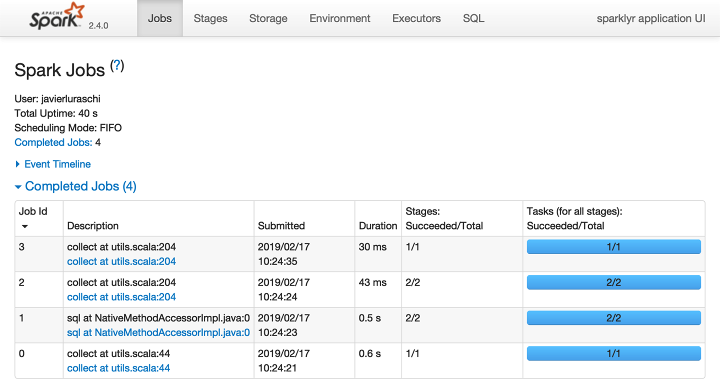
\includegraphics{figures/2_1.png}
\caption{图2-1. Apache Spark网络接口}
\end{figure}

打印\texttt{cars}数据集会收集几行记录并展示到R控制台。你可以在Spark网络接口中看到,一个作业用于在Spark中收集这个信息。你可以可选择Storage标签,查看Spark内存中的\texttt{mtcars}数据集,如图2-2所示。

注意,根据Fraction
Cached列100\%取值,这个数据集完全加载到了内存中。因此,根据Size in
Memory列,你可以准确的看到这个数据集使用了多少内存。

\begin{figure}
\centering
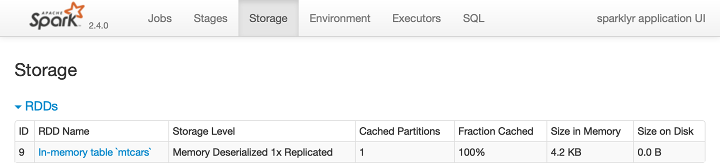
\includegraphics{figures/2_2.png}
\caption{图2-2. Apache Spark网络接口的Storage标签}
\end{figure}

Executors标签,如图2-3所示,提供了集群资源的总览。对于本地连接,你只能看到一个2
GB内存的,384
MB计算内存的Spark工作节点。在第九章中国,你会看到,如何请求更过的计算实例和资源,以及内存如何分配。

\begin{figure}
\centering
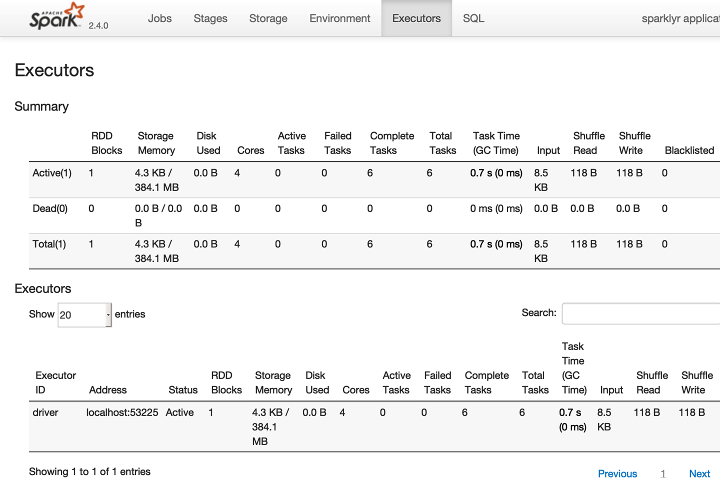
\includegraphics{figures/2_3.png}
\caption{图2-3. Apache Spark网络接口的Executors标签}
\end{figure}

最后一个要介绍的标签是Environment标签,如图2-4所示;这个标签列出了所有Spark应用的设置,我们会在第九章中介绍。你可以看到,大部分设置不需要明确的配置,但是要在大规模数据上顺利运行,你还是要熟悉这些配置。

\begin{figure}
\centering
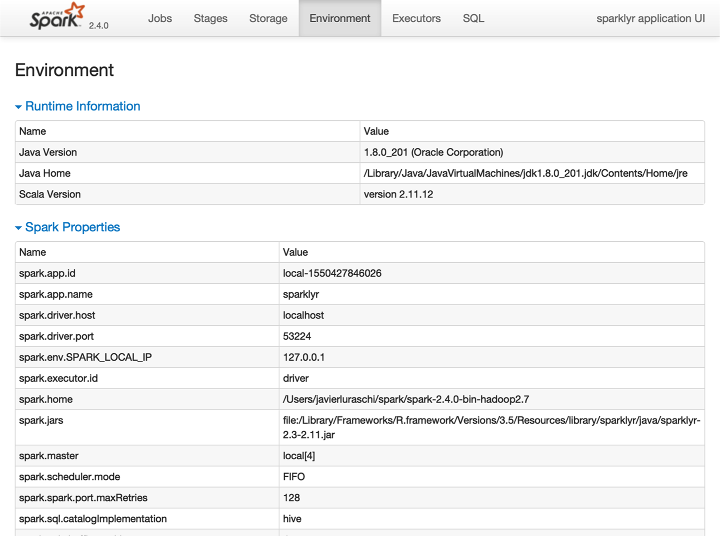
\includegraphics{figures/2_4.png}
\caption{图2-4. Apache Spark网络接口的Environment标签}
\end{figure}

然后,你可以使用小的数据子集进行练习。我们会在第三章中国详细介绍。

\hypertarget{ux5206ux6790}{%
\subsubsection{分析}\label{ux5206ux6790}}

在R中使用Spark分析数据,你可以使用SQL(结构化查询语句)或者\texttt{dplyr}(数据操作语法)。你可以通过\texttt{DBI}程序包使用SQL。例如,要计算我们的\texttt{cars}数据集中有多少记录,我们可以运行如下代码:

\begin{Shaded}
\begin{Highlighting}[]
\KeywordTok{library}\NormalTok{(DBI)}
\KeywordTok{dbGetQuery}\NormalTok{(sc, }\StringTok{"SELECT count(*) FROM mtcars"}\NormalTok{)}
\KeywordTok{count}\NormalTok{(}\DecValTok{1}\NormalTok{)}
\DecValTok{1} \DecValTok{32}
\end{Highlighting}
\end{Shaded}

使用\texttt{dplyr}的时候,需要的代码更少。而且通常比SQL容易的多。这也是为什么本书不用SQL的原因,但是,如果你对SQL很熟悉,这也是备选方案。例如,\texttt{dplyr}中计算行数要更简洁,且易于理解:

\begin{Shaded}
\begin{Highlighting}[]
\KeywordTok{library}\NormalTok{(dplyr)}
\KeywordTok{count}\NormalTok{(cars)}
\CommentTok{# Source: spark<?> [?? x 1]}
\NormalTok{n}
\OperatorTok{<}\NormalTok{dbl}\OperatorTok{>}
\DecValTok{1} \DecValTok{32}
\end{Highlighting}
\end{Shaded}

一般情况下,我们通常首先使用\texttt{dplyr}做Spark中的数据分析,然后进行采样和列维度的子集选取。最后一步是从Spark中收集数据,并在R中做进一步数据处理,例如数据可视化。让我们运行一个非常简单的数据分析例子,包括对Spark中\texttt{cars}数据集选取,采样,绘制图形:

\begin{Shaded}
\begin{Highlighting}[]
\KeywordTok{select}\NormalTok{(cars, hp, mpg) }\OperatorTok\StringTok{ }\KeywordTok{sample_n}\NormalTok{(}\DecValTok{100}\NormalTok{) }\OperatorTok\StringTok{ }\KeywordTok{collect}\NormalTok{() }\OperatorTok\StringTok{ }\KeywordTok{plot}\NormalTok{()}
\end{Highlighting}
\end{Shaded}

图2-5看到,随着汽车马力的增加,它的每加仑英里数燃料效率在降低。尽管这个分析很深刻,但是要定量预测增加的马力影响多少燃料效率也并不容易。建模工作可以帮助我们解决这个问题。

\begin{figure}
\centering
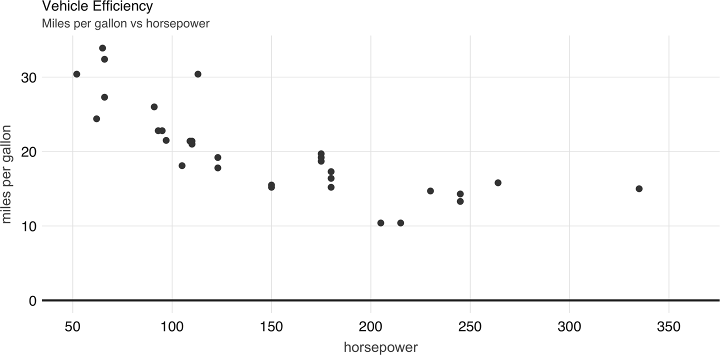
\includegraphics{figures/2_5.png}
\caption{图2-5. 马力vs每加仑英里数}
\end{figure}

\hypertarget{ux5efaux6a21}{%
\subsubsection{建模}\label{ux5efaux6a21}}

尽管数据分析可以让你快速理解数据,构建数学模型描述和泛化数据集也非常有用。在第一章中,你学习了机器学习和数据科学领域使用数学模型进行预测和发现重要的观点。例如,我们可以使用线性模型估计燃料效率和马力的关系:

\begin{Shaded}
\begin{Highlighting}[]
\NormalTok{model <-}\StringTok{ }\KeywordTok{ml_linear_regression}\NormalTok{(cars, mpg }\OperatorTok{~}\StringTok{ }\NormalTok{hp)}
\NormalTok{model}
\NormalTok{Formula}\OperatorTok{:}\StringTok{ }\NormalTok{mpg }\OperatorTok{~}\StringTok{ }\NormalTok{hp}
\NormalTok{Coefficients}\OperatorTok{:}
\NormalTok{(Intercept) hp}
\FloatTok{30.09886054} \FloatTok{-0.06822828}
\end{Highlighting}
\end{Shaded}

现在我们可以使用这个模型预测不在原始数据集中的值。例如,我们可以添加马力大于250的数据,并可视化预测的值,如图2-6所示。

\begin{Shaded}
\begin{Highlighting}[]
\NormalTok{model }\OperatorTok\StringTok{ }\KeywordTok{ml_predict}\NormalTok{(}\KeywordTok{copy_to}\NormalTok{(sc, }\KeywordTok{data.frame}\NormalTok{(}\DataTypeTok{hp =} \DecValTok{250} \OperatorTok{+}\StringTok{ }\DecValTok{10} \OperatorTok{*}\StringTok{ }\DecValTok{1}\OperatorTok{:}\DecValTok{10}\NormalTok{))) }\OperatorTok\StringTok{ }\KeywordTok{transmute}\NormalTok{(}\DataTypeTok{hp =}\NormalTok{ hp, }
    \DataTypeTok{mpg =}\NormalTok{ prediction) }\OperatorTok\StringTok{ }\KeywordTok{full_join}\NormalTok{(}\KeywordTok{select}\NormalTok{(cars, hp, mpg)) }\OperatorTok\StringTok{ }\KeywordTok{collect}\NormalTok{() }\OperatorTok\StringTok{ }\KeywordTok{plot}\NormalTok{()}
\end{Highlighting}
\end{Shaded}

\begin{figure}
\centering
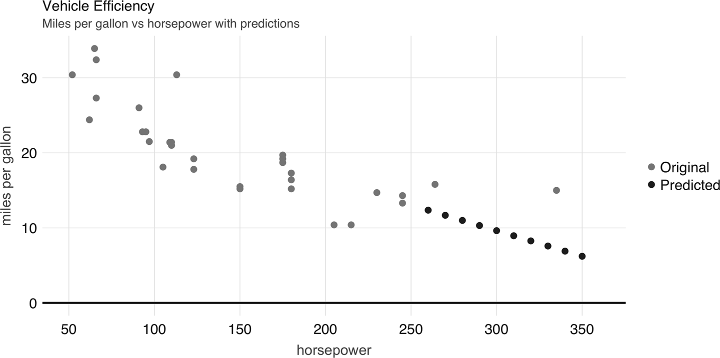
\includegraphics{figures/2_6.png}
\caption{图2-6. 马力vs每加仑英里数预测结果}
\end{figure}

尽管前面的例子缺少建模中所用的诸多技术,但是也足以作为一个简单的例子简要介绍Spark的建模能力。我们会在第四章中介绍所有Spark的模型,技术和最佳实践。

\hypertarget{ux6570ux636e}{%
\subsubsection{数据}\label{ux6570ux636e}}

简单起见,我们确实把\texttt{mtcars}数据集复制给了Spark。但是,一般情况下数据通常不在Saprk中。相反,数据要从已有的数据源中读取,格式也多种多样,例如纯文本,CSV,JSON,Java数据库连接JDBC和其它。我们会在第八章中详细介绍这些内容。例如,我们可以把\texttt{cars}数据集输出为CSV文件:

\begin{Shaded}
\begin{Highlighting}[]
\KeywordTok{spark_write_csv}\NormalTok{(cars, }\StringTok{"cars.csv"}\NormalTok{)}
\end{Highlighting}
\end{Shaded}

实际工作中,我们会从分布式存储系统例如HDFS中读取已有额数据集,但是我们也可以从本地文件系统中读取数据:

\begin{Shaded}
\begin{Highlighting}[]
\NormalTok{cars <-}\StringTok{ }\KeywordTok{spark_read_csv}\NormalTok{(sc, }\StringTok{"cars.csv"}\NormalTok{)}
\end{Highlighting}
\end{Shaded}

\hypertarget{ux6269ux5c55}{%
\subsubsection{扩展}\label{ux6269ux5c55}}

R以其活跃的程序包作者社区而著名。同样的,许多Spark和R扩展已经编程实现,并随时可用,只是数量较R社区中的少些。第十章会介绍许多有趣的程序包支持高级建模,图分析,深度学习数据预处理等等。

例如,\texttt{sparkly.nested}扩展是R的一个程序包,允许\texttt{sparklyr}管理包含嵌套信息的取值。常见的用例是,包含嵌套列表的JSON文件,需要在有意义的数据分析前做预处理。要使用这个扩展,我们首先需要按照如下代码安装:

\begin{Shaded}
\begin{Highlighting}[]
\KeywordTok{install.packages}\NormalTok{(}\StringTok{"sparklyr.nested"}\NormalTok{)}
\end{Highlighting}
\end{Shaded}

然后,我们可以使用\texttt{sparklyr.nested}扩展,根据气缸数,对所有的马力数据点分组:
points over the number of cylinders:

\begin{Shaded}
\begin{Highlighting}[]
\NormalTok{sparklyr.nested}\OperatorTok{::}\KeywordTok{sdf_nest}\NormalTok{(cars, hp) }\OperatorTok
\KeywordTok{group_by}\NormalTok{(cyl) }\OperatorTok
\KeywordTok{summarise}\NormalTok{(}\DataTypeTok{data =} \KeywordTok{collect_list}\NormalTok{(data))}
\CommentTok{# Source: spark<?> [?? x 2]}
\NormalTok{cyl data}
\OperatorTok{<}\NormalTok{int}\OperatorTok{>}\StringTok{ }\ErrorTok{<}\NormalTok{list}\OperatorTok{>}
\DecValTok{1} \DecValTok{6} \OperatorTok{<}\NormalTok{list [}\DecValTok{7}\NormalTok{]}\OperatorTok{>}
\DecValTok{2} \DecValTok{4} \OperatorTok{<}\NormalTok{list [}\DecValTok{11}\NormalTok{]}\OperatorTok{>}
\DecValTok{3} \DecValTok{8} \OperatorTok{<}\NormalTok{list [}\DecValTok{14}\NormalTok{]}\OperatorTok{>}
\end{Highlighting}
\end{Shaded}

尽管嵌套数据不太容易读取,但是在借助\texttt{spark\_read\_json()}和\texttt{spark\_write\_json()}函数处理诸如JSON的嵌套数据格式的时候,确实存在这样的需求。

\hypertarget{ux5206ux5e03ux5f0fr}{%
\subsubsection{分布式R}\label{ux5206ux5e03ux5f0fr}}

对于某些情况下,个别Spark的功能不能实现,或者扩展没有开发完成,你可以考虑把R代码发布到Spark集群上。这是一个强大的工具,但是也带了额外的复杂性。所以你应该把它做为最后的方案。

假设我们需要四舍五入数据集中所有列的取值。一个方法是运行R代码,执行\texttt{round()}函数:

\begin{Shaded}
\begin{Highlighting}[]
\NormalTok{cars }\OperatorTok\StringTok{ }\KeywordTok{spark_apply}\NormalTok{(}\OperatorTok{~}\KeywordTok{round}\NormalTok{(.x))}
\CommentTok{# Source: spark<?> [?? x 11]}
\NormalTok{mpg cyl disp hp drat wt qsec vs am gear carb}
\OperatorTok{<}\NormalTok{dbl}\OperatorTok{>}\StringTok{ }\ErrorTok{<}\NormalTok{dbl}\OperatorTok{>}\StringTok{ }\ErrorTok{<}\NormalTok{dbl}\OperatorTok{>}\StringTok{ }\ErrorTok{<}\NormalTok{dbl}\OperatorTok{>}\StringTok{ }\ErrorTok{<}\NormalTok{dbl}\OperatorTok{>}\StringTok{ }\ErrorTok{<}\NormalTok{dbl}\OperatorTok{>}\StringTok{ }\ErrorTok{<}\NormalTok{dbl}\OperatorTok{>}\StringTok{ }\ErrorTok{<}\NormalTok{dbl}\OperatorTok{>}\StringTok{ }\ErrorTok{<}\NormalTok{dbl}\OperatorTok{>}\StringTok{ }\ErrorTok{<}\NormalTok{dbl}\OperatorTok{>}\StringTok{ }\ErrorTok{<}\NormalTok{dbl}\OperatorTok{>}
\DecValTok{1} \DecValTok{21} \DecValTok{6} \DecValTok{160} \DecValTok{110} \DecValTok{4} \DecValTok{3} \DecValTok{16} \DecValTok{0} \DecValTok{1} \DecValTok{4} \DecValTok{4}
\DecValTok{2} \DecValTok{21} \DecValTok{6} \DecValTok{160} \DecValTok{110} \DecValTok{4} \DecValTok{3} \DecValTok{17} \DecValTok{0} \DecValTok{1} \DecValTok{4} \DecValTok{4}
\DecValTok{3} \DecValTok{23} \DecValTok{4} \DecValTok{108} \DecValTok{93} \DecValTok{4} \DecValTok{2} \DecValTok{19} \DecValTok{1} \DecValTok{1} \DecValTok{4} \DecValTok{1}
\DecValTok{4} \DecValTok{21} \DecValTok{6} \DecValTok{258} \DecValTok{110} \DecValTok{3} \DecValTok{3} \DecValTok{19} \DecValTok{1} \DecValTok{0} \DecValTok{3} \DecValTok{1}
\DecValTok{5} \DecValTok{19} \DecValTok{8} \DecValTok{360} \DecValTok{175} \DecValTok{3} \DecValTok{3} \DecValTok{17} \DecValTok{0} \DecValTok{0} \DecValTok{3} \DecValTok{2}
\DecValTok{6} \DecValTok{18} \DecValTok{6} \DecValTok{225} \DecValTok{105} \DecValTok{3} \DecValTok{3} \DecValTok{20} \DecValTok{1} \DecValTok{0} \DecValTok{3} \DecValTok{1}
\DecValTok{7} \DecValTok{14} \DecValTok{8} \DecValTok{360} \DecValTok{245} \DecValTok{3} \DecValTok{4} \DecValTok{16} \DecValTok{0} \DecValTok{0} \DecValTok{3} \DecValTok{4}
\DecValTok{8} \DecValTok{24} \DecValTok{4} \DecValTok{147} \DecValTok{62} \DecValTok{4} \DecValTok{3} \DecValTok{20} \DecValTok{1} \DecValTok{0} \DecValTok{4} \DecValTok{2}
\DecValTok{9} \DecValTok{23} \DecValTok{4} \DecValTok{141} \DecValTok{95} \DecValTok{4} \DecValTok{3} \DecValTok{23} \DecValTok{1} \DecValTok{0} \DecValTok{4} \DecValTok{2}
\DecValTok{10} \DecValTok{19} \DecValTok{6} \DecValTok{168} \DecValTok{123} \DecValTok{4} \DecValTok{3} \DecValTok{18} \DecValTok{1} \DecValTok{0} \DecValTok{4} \DecValTok{4}
\CommentTok{# … with more rows}
\end{Highlighting}
\end{Shaded}

如果你是R语言高手,你会倾向于使用\texttt{spark\_apply()}处理一切。但是最好别这样!\texttt{spark\_apply()}
适用于Spark能力受限的高级情形。你会了解到如何执行合适的数据分析和建模,而不用把R代码分发给你的集群。

\hypertarget{ux6d41ux5f0fux8ba1ux7b97}{%
\subsubsection{流式计算}\label{ux6d41ux5f0fux8ba1ux7b97}}

虽然处理大量静态数据是Spark的典型应用场景,但是Spark也可以处理实时动态数据集。某些应用中确实有这样的需求。你可以把一个流式数据集看做一个持续更新数据的静态数据源,例如股票市场报价。流式数据通常从Kafka(一个开源的流式数据处理软件平台)或分布式存储中读取。

要体验流式计算,首先创建一个input/文件夹,放入一些流式计算所需的输入数据:

\begin{Shaded}
\begin{Highlighting}[]
\KeywordTok{dir.create}\NormalTok{(}\StringTok{"input"}\NormalTok{)}
\KeywordTok{write.csv}\NormalTok{(mtcars, }\StringTok{"input/cars_1.csv"}\NormalTok{, }\DataTypeTok{row.names =}\NormalTok{ F)}
\end{Highlighting}
\end{Shaded}

然后,定义一个作业流,处理来自input/文件夹的数据,执行R代码定义的转换,并输出到一个output/文件夹:

\begin{Shaded}
\begin{Highlighting}[]
\NormalTok{stream <-}\StringTok{ }\KeywordTok{stream_read_csv}\NormalTok{(sc, }\StringTok{"input/"}\NormalTok{) }\OperatorTok\StringTok{ }\KeywordTok{select}\NormalTok{(mpg, cyl, disp) }\OperatorTok\StringTok{ }\KeywordTok{stream_write_csv}\NormalTok{(}\StringTok{"output/"}\NormalTok{)}
\end{Highlighting}
\end{Shaded}

实时数据一开始输入,input/文件夹几乎同时开始处理,并在output/文件夹中存入新的转换数据文件。因为输入文件夹只有一个文件,输出文件夹也只包含一个经过\texttt{spark\_apply()}转换的文件。

\begin{Shaded}
\begin{Highlighting}[]
\KeywordTok{dir}\NormalTok{(}\StringTok{"output"}\NormalTok{, }\DataTypeTok{pattern =} \StringTok{".csv"}\NormalTok{)}
\NormalTok{[}\DecValTok{1}\NormalTok{] }\StringTok{"part-00000-eece04d8-7cfa-4231-b61e-f1aef8edeb97-c000.csv"}
\end{Highlighting}
\end{Shaded}

到目前为止,这些操作和静态数据的处理很像。但是,我们可以持续添加input/文件夹中的文件,Spark会自动的并行处理数据。让我们添加一个新的文件,检查是否可以自动处理:

\begin{Shaded}
\begin{Highlighting}[]
\CommentTok{# Write more data into the stream source}
\KeywordTok{write.csv}\NormalTok{(mtcars, }\StringTok{"input/cars_2.csv"}\NormalTok{, }\DataTypeTok{row.names =}\NormalTok{ F)}
\end{Highlighting}
\end{Shaded}

等待几秒,确认Spark作业流处理了数据:

\begin{Shaded}
\begin{Highlighting}[]
\CommentTok{# Check the contents of the stream destination}
\KeywordTok{dir}\NormalTok{(}\StringTok{"output"}\NormalTok{, }\DataTypeTok{pattern =} \StringTok{".csv"}\NormalTok{)}
\NormalTok{[}\DecValTok{1}\NormalTok{] }\StringTok{"part-00000-2d8e5c07-a2eb-449d-a535-8a19c671477d-c000.csv"}
\NormalTok{[}\DecValTok{2}\NormalTok{] }\StringTok{"part-00000-eece04d8-7cfa-4231-b61e-f1aef8edeb97-c000.csv"}
\end{Highlighting}
\end{Shaded}

然后你应该终止作业流:

\begin{Shaded}
\begin{Highlighting}[]
\KeywordTok{stream_stop}\NormalTok{(stream)}
\end{Highlighting}
\end{Shaded}

你可以使用\texttt{dplyr},SQL,Spark模型,或者分布式R分析实时数据流。在第十二章中,我们会详细介绍分析实时数据所需的所有有意思的转换。

\hypertarget{ux65e5ux5fd7}{%
\subsubsection{日志}\label{ux65e5ux5fd7}}

日志记录肯定比实时数据处理要无聊。但是,它是你应该熟悉的工具。日志是一份文本文件,Spark可以追加集群中任务执行的相关信息。对于本地集群,我们运行如下代码,获取所有相关日志:

\begin{Shaded}
\begin{Highlighting}[]
\KeywordTok{spark_log}\NormalTok{(sc)}
\DecValTok{18}\OperatorTok{/}\DecValTok{10}\OperatorTok{/}\DecValTok{09} \DecValTok{19}\OperatorTok{:}\DecValTok{41}\OperatorTok{:}\DecValTok{46}\NormalTok{ INFO Executor}\OperatorTok{:}\StringTok{ }\NormalTok{Finished task }\FloatTok{0.0} \ControlFlowTok{in}\NormalTok{ stage }\FloatTok{5.0}\NormalTok{ (TID }\DecValTok{5}\NormalTok{)...}
\DecValTok{18}\OperatorTok{/}\DecValTok{10}\OperatorTok{/}\DecValTok{09} \DecValTok{19}\OperatorTok{:}\DecValTok{41}\OperatorTok{:}\DecValTok{46}\NormalTok{ INFO TaskSetManager}\OperatorTok{:}\StringTok{ }\NormalTok{Finished task }\FloatTok{0.0} \ControlFlowTok{in}\NormalTok{ stage }\DecValTok{5}\NormalTok{.}\DecValTok{0}\NormalTok{...}
\DecValTok{18}\OperatorTok{/}\DecValTok{10}\OperatorTok{/}\DecValTok{09} \DecValTok{19}\OperatorTok{:}\DecValTok{41}\OperatorTok{:}\DecValTok{46}\NormalTok{ INFO TaskSchedulerImpl}\OperatorTok{:}\StringTok{ }\NormalTok{Removed TaskSet }\FloatTok{5.0}\NormalTok{, whose...}
\DecValTok{18}\OperatorTok{/}\DecValTok{10}\OperatorTok{/}\DecValTok{09} \DecValTok{19}\OperatorTok{:}\DecValTok{41}\OperatorTok{:}\DecValTok{46}\NormalTok{ INFO DAGScheduler}\OperatorTok{:}\StringTok{ }\NormalTok{ResultStage }\DecValTok{5}\NormalTok{ (collect at utils...}
\DecValTok{18}\OperatorTok{/}\DecValTok{10}\OperatorTok{/}\DecValTok{09} \DecValTok{19}\OperatorTok{:}\DecValTok{41}\OperatorTok{:}\DecValTok{46}\NormalTok{ INFO DAGScheduler}\OperatorTok{:}\StringTok{ }\NormalTok{Job }\DecValTok{3}\NormalTok{ finished}\OperatorTok{:}\StringTok{ }\NormalTok{collect at utils...}
\end{Highlighting}
\end{Shaded}

我们也可以具体的日志记录,比如包含\texttt{sparklyr}的记录。使用\texttt{filter}参数,运行如下代码:

\begin{Shaded}
\begin{Highlighting}[]
\KeywordTok{spark_log}\NormalTok{(sc, }\DataTypeTok{filter =} \StringTok{"sparklyr"}\NormalTok{)}
\CommentTok{## 18/10/09 18:53:23 INFO SparkContext: Submitted application: sparklyr 18/10/09}
\CommentTok{## 18:53:23 INFO SparkContext: Added JAR...  18/10/09 18:53:27 INFO Executor:}
\CommentTok{## Fetching spark://localhost:52930/...  18/10/09 18:53:27 INFO Utils: Fetching}
\CommentTok{## spark://localhost:52930/...  18/10/09 18:53:27 INFO Executor: Adding}
\CommentTok{## file:/private/var/folders/...}
\end{Highlighting}
\end{Shaded}

多数情况下,你不必操心Spark日志,除非你需要排查一个失败的计算任务。此时,日志是无价之宝。切记!

\hypertarget{ux65adux5f00ux8fdeux63a5}{%
\subsection{断开连接}\label{ux65adux5f00ux8fdeux63a5}}

对于本地集群(以及任何集群),你应该在完成数据处理后,使用如下代码断开连接:

\begin{Shaded}
\begin{Highlighting}[]
\KeywordTok{spark_disconnect}\NormalTok{(sc)}
\end{Highlighting}
\end{Shaded}

这些操作会终止集群连接和集群任务。如果有多个Spark连接在工作,或者连接实例\texttt{sc}不再可用,你也可以使用如下命令,断开所有的Spark连接:

\begin{Shaded}
\begin{Highlighting}[]
\KeywordTok{spark_disconnect_all}\NormalTok{()}
\end{Highlighting}
\end{Shaded}

注意,退出R或者RStudio,或者重启R进程,也会引起Spark连接终止,进而终止Spark集群并把没有明确保存的数据放在缓存。

\hypertarget{ux4f7fux7528rstudio}{%
\subsubsection{使用RStudio}\label{ux4f7fux7528rstudio}}

既然使用RStudio运行R非常普遍,\texttt{sparklyr}也提供了RStudio扩展来帮助简化工作流,提高Rstudio中使用Spark的生产效率。如果你不熟悉RStudio,可以快速浏览依一下``使用Rstudio''部分。一些扩展非常值得关注。

首先,不用Rstudio控制台的\texttt{spark\_connect()}建立连接,你可以用Connections标签下的New
Connection操作,然后选取Spark
connection,打开图2-7的对话窗口。你可定制版本号和连接配置,生成正确的\texttt{spark\_connect()}命令,并在R控制台中执行。

\begin{figure}
\centering
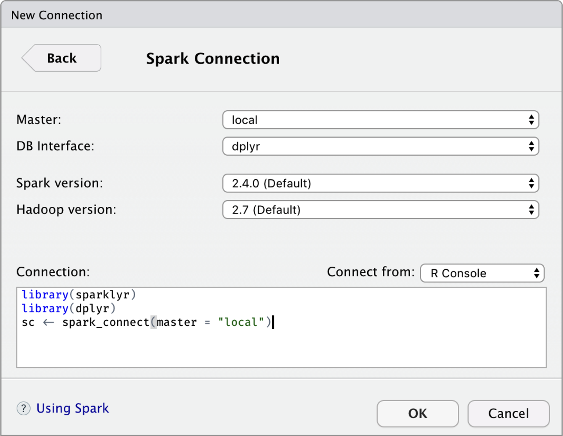
\includegraphics{figures/2_7.png}
\caption{图2-7. RStudio中新建Spark连接对话窗口}
\end{figure}

连接到Spark后,RStudio在Connections标签中展示了可用的数据集,如图2-8所示。这是跟踪可用数据集很有用的方法,也提供了探查它们的简便方式。

\begin{figure}
\centering
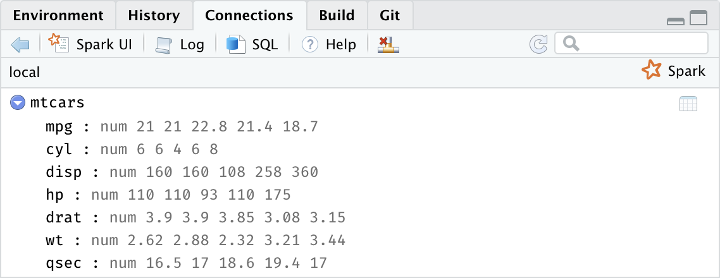
\includegraphics{figures/2_8.png}
\caption{图2-8. RStudio的Connections标签}
\end{figure}

另外,活跃的连接提供了如下定制的操作:

\begin{itemize}
\item
  Spark UI

  打开Spark网络接口,\texttt{spark\_web(sc)}快捷操作。
\item
  日志

  打开Spark网络日志,\texttt{spark\_log(sc)}快捷操作。
\item
  SQL

  打开新的SQL查询。更多关于\texttt{DBI}和SQL支持额信息,可以查看第三章。
\item
  帮助

  在新的浏览器窗口中打开参考文档。
\item
  断开

  断开Spark连接,\texttt{spark\_disconnect(sc)}快捷操作。
\end{itemize}

本书的后边章节会使用纯R代码。本书中的代码都在R环境中运行。是在R控制台,Rstudio,Jupyter
Notebooks,还是其它支持R代码的工具中运行R代码,取决于你个人的需要。

\hypertarget{ux8d44ux6e90}{%
\subsection{资源}\label{ux8d44ux6e90}}

我们已经花了很大的精力简化上手过程,不过还有许多其它资源可以帮助你解决具体的上手问题。通常,这些资源会介绍更广泛的Spark和R社区,帮助你找到具体的答案,讨论某个话题,与经常使用Spark和R的用户沟通:

\begin{itemize}
\item
  文档

  托管在RStudio的Spark网站的文档站点应该是了解更多在R中用Spark知识的首要选择。文档会对示例,引用函数和其他更多相关资源保存持续更新。
\item
  博客

  要获取最新的重大\texttt{sparklyr}通知,你可以关注Rstudio博客。 blog.
\item
  社区

  对于常见的\texttt{sparklyr}问题,你可以在RStudio社区发布帖子,并带上标签\texttt{sparklyr}。
\item
  Stack Overflow

  对于常见的Spark问题,Stack
  Overflow是一个很棒的资源,它也包含很多关于\texttt{sparklyr}的话题。
\item
  GitHub

  如果确定一些代码需要修改,你可以新建一个GitHub
  issue,或者给我们发送一个pull请求。
\item
  Gitter

  对于紧急的问题,或者需要时常保持联系,你可以通过Gitter和我们沟通。
\end{itemize}

\hypertarget{ux5c0fux7ed3-1}{%
\subsection{小结}\label{ux5c0fux7ed3-1}}

在本章中,你学到了使用Spark的预备操作。你已经看到如何使用\texttt{spark\_connect()}连接Spark,使用\texttt{spark\_install()}安装本地集群,使用\texttt{spark\_web(sc)}和\texttt{spark\_log(sc)}加载简单的数据集,启动网络接口和展示日志,使用RStudio的\texttt{spark\_disconnect()}断开连接。最后,我们介绍了\texttt{sparklyr}提供的Rstudio扩展。

现在,我们希望你准备好使用Spark和R分析真实数据和建模问题。这些内容会在接下来两章介绍。第三章会介绍数据分析,一个探查,清洗和转换数据的过程,达到发现有用的信息的目的。第四章,建模,可以看做是数据分析的一部分。但是适合独立成章,以便真正阐述和利用Spark的建模功能。

\begin{center}\rule{0.5\linewidth}{\linethickness}\end{center}

\hypertarget{ux7b2c3ux7ae0-ux5206ux6790}{%
\section{第3章 分析}\label{ux7b2c3ux7ae0-ux5206ux6790}}

\begin{quote}
First lesson: stick them with the pointy end. ---Jon Snow
\end{quote}

之前的章节主要介绍Spark和R,可以让你快速熟悉和鼓励尝试基础的数据分析流程。但是,我们并没有介绍什么是数据分析,尤其是Spark中的数据分析。
我们介绍了本书中需要用到的工具,它们有助于你更多的关注学习而不是排查问题。

本章会介绍使用Spark和R进行数据分析的工具和概念。需要注意的是,这些工具和你只使用R的时候一样!这并非偶然。我们只是希望数据科学家能够屏蔽一些技术细节,而只使用自己熟知和喜欢的程序库,并且确实在Spark框架下可行。现在我们离这个目标还有点距离,但是并不远。所以,你会在本章学到一些广泛使用的R程序包和实际操作来进行数据分析------\texttt{dplyr},\texttt{ggplot2},\texttt{formulas},\texttt{rmarkdown}等,这些程序包在Spark框架下依然有效。

第四章会关注创建统计模型来预测,估计和描述数据集。但是首先,我们从分析工作开始!

\hypertarget{ux6982ux8ff0-2}{%
\subsection{概述}\label{ux6982ux8ff0-2}}

数据分析项目的主要目标是理解数据到底要告诉我们什么,希望能够给出一个具体问题的答案。大部分数据分析项目遵循一些步骤,如图3-1所示。

如图所示,我们首先把数据引入主要分析流程。这个流程会对通过各种数据转换,例如数据合并,完成\emph{数据操作}。然后,我们会对数据\emph{可视化},以便看到数据的关系和趋势。要获得更深的理解,我们可以用一个或者多个统计模型集合数据。这会帮助我们找出相关模式在数据集上是否成立。最后,结果可以以公开的形式或者私密的形式和同事和相关人员沟通。

\begin{figure}
\centering
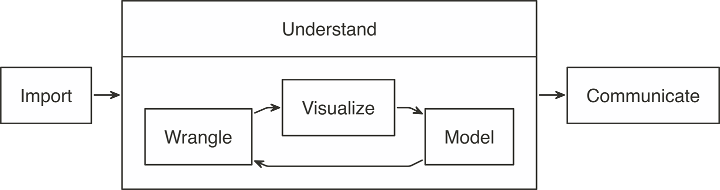
\includegraphics{figures/3_1.png}
\caption{图3-1. 数据分析一般步骤}
\end{figure}

当处理小规模数据集,也就是内存允许的数据集时,我们可以按照R语言的步骤执行,不用使用Spark。但是,当数据及无法放入内存,或者计算太慢时,我们可以结合Spark一个优化这些步骤。但是如何优化呢?

对于数据分析师而言,理想的方法是让Spark做它擅长的事情。Spark是并行计算的引擎,可以在大数据集上工作,并提供SQL查询引擎和建模所用的各种库。你可以使用这些技术执行与R大部分相同的操作。这些操作,包括数据选取,转换,建模。
另外,Spark包含了一些执行特殊计算的工具,例如图分析,流式处理和其他等。现在,我们跳过这些非表格数据集,留在后面的章节介绍。

你可以使用Spark进行数据\emph{导入},\emph{操作}和\emph{建模}。你也可以做一部分可视化工作,后边会介绍这一内容。最终目的是要使用R告诉Spark要做什么数据操作,并把结果返回给R。如图3-2所示,理想的流程可以\emph{推动计算(pushes
compute)} 到Spark集群中,并\emph{收集结果(collects results)}返回给。

\begin{figure}
\centering
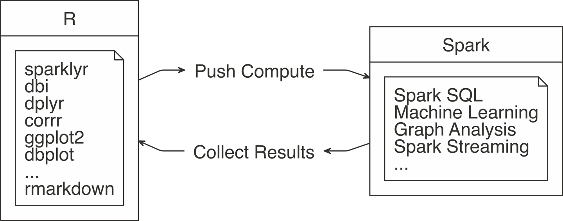
\includegraphics{figures/3_2.png}
\caption{图3-2. Spark进行数据计算,R收集计算结果}
\end{figure}

\texttt{sparklyr}程序包助力实现``推动计算,收集结果''的原则。其大部分函数都是Spark
API调用的顶层封装。这可以让我们利用Spark的分析组件,而不是R的分析组件。例如,当你需要拟合线性回归模型的时候,不要使用R的熟知的\texttt{lm()}函数,你应该使用Spark对应的\texttt{ml\_linear\_regression()}函数。
这个R函数会调用Spark创建模型。图3-3给出了具体的例子。

\begin{figure}
\centering
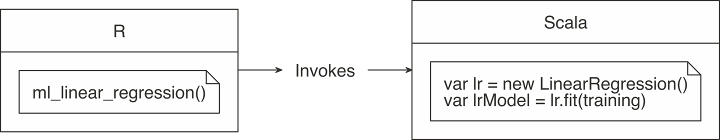
\includegraphics{figures/3_3.png}
\caption{图3-3. R函数调用Spark功能}
\end{figure}

对于更常见的数据任务,\texttt{sparklyr}提供了\texttt{dplyr}的强大支持。这就意味着,你可以使用R中已经熟知的\texttt{dplyr}操作,然后\texttt{sparklyr}和\texttt{dplyr}会把这些操作转换成Spark
SQL语句。这些语句通常比SQL语句更加紧凑,易读(见图3-4)。所以,如果你对R和\texttt{dplyr}很熟悉,无需过多学习。这可能让人觉得有点虎头蛇尾。的确有点这种感觉。但是,可以专注学习大规模计算技能也是很棒的体验。

\begin{figure}
\centering
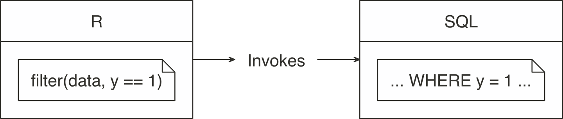
\includegraphics{figures/3_4.png}
\caption{图3-4. \texttt{dplyr}在Spark中执行SQL语句}
\end{figure}

为了边学边练,本章后边的代码使用简单的练习,可以在本地Spark集群上运行。这样,你可以在自己的电脑上重复代码。确保\texttt{sparklyr}可以使用,第二章已经有过相关介绍。

本章会使用一些你可能还没有安装的包,所以确保以下程序包通过如下命令安装成功:

\begin{Shaded}
\begin{Highlighting}[]
\KeywordTok{install.packages}\NormalTok{(}\StringTok{"ggplot2"}\NormalTok{)}
\KeywordTok{install.packages}\NormalTok{(}\StringTok{"corrr"}\NormalTok{)}
\KeywordTok{install.packages}\NormalTok{(}\StringTok{"dbplot"}\NormalTok{)}
\KeywordTok{install.packages}\NormalTok{(}\StringTok{"rmarkdown"}\NormalTok{)}
\end{Highlighting}
\end{Shaded}

首先,加载\texttt{sparklyr}和\texttt{dplyr}程序包,并打开新的本地连接。

\begin{Shaded}
\begin{Highlighting}[]
\KeywordTok{library}\NormalTok{(sparklyr)}
\KeywordTok{library}\NormalTok{(dplyr)}
\NormalTok{sc <-}\StringTok{ }\KeywordTok{spark_connect}\NormalTok{(}\DataTypeTok{master =} \StringTok{"local"}\NormalTok{, }\DataTypeTok{version =} \StringTok{"2.3"}\NormalTok{)}
\end{Highlighting}
\end{Shaded}

环境已经可以用了,下面我们要导入数据,进行分析。

\hypertarget{ux6570ux636eux5bfcux5165}{%
\subsection{数据导入}\label{ux6570ux636eux5bfcux5165}}

使用Spark和R的时候,你需要使用不同的导入数据方法。通常,导入意味着R会读取文件,并加载到内存中。而使用Spark的时候,数据导入Spark,而不是R。在图3-5中,我们可以看到,数据源是如何与Spark连接而不是和R连接的。

\begin{figure}
\centering
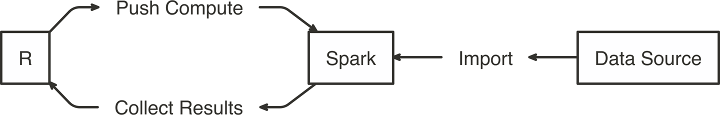
\includegraphics{figures/3_5.png}
\caption{图3-5. 数据导入到Spark,而不是R}
\end{figure}

\begin{quote}
当你进行分析大规模数据集的时候,Spark集群中大部分所需的数据都可以进行操作(通常允许用户通过hive表或直接请求文件系统而实现)。第八章或详细介绍这些内容。
\end{quote}

不要把所有的数据都导入Spark中,你可以让Spark请求数据源,而不是导入数据。你应该根据机器速度和性能做出一个决定。给Spark进程导入所有的数据会引起一次性内存支出,因为Spark需要等待所有的数据都加载好了才能分析。而如果没有导入数据,你通过会遇到每次Spark操作的支出问题,因为Spark需要从集群存储,通常是磁盘驱动器中获取数据子集。这通常要比从Spark内存中读取数据要慢得多。第九章会详细介绍这一话题。

让我们首先使用\texttt{copy\_to()}给Spark导入数据,准备有个带有数据的进程。你也可以从各种格式的分布式文件中导入数据。相关内容会在第八章中介绍。

\begin{Shaded}
\begin{Highlighting}[]
\NormalTok{cars <-}\StringTok{ }\KeywordTok{copy_to}\NormalTok{(sc, mtcars)}
\end{Highlighting}
\end{Shaded}

\begin{quote}
使用真实集群的时候,你应该只对小的R数据表格使用\texttt{copy\_to()}进行转换,大的数据表格转换应该使用专门的数据转换工具。
\end{quote}

现在Spark可以请求数据,你可以轻松的进行数据转换。下一节会介绍如何在Spark中使用\texttt{dplyr}转换数据。

\hypertarget{ux6570ux636eux64cdux4f5c}{%
\subsection{数据操作}\label{ux6570ux636eux64cdux4f5c}}

数据操作利用数据转换理解数据。它通常指的是把``原始''数据转换成其他格式的数据,并试图利于后续数据分析的过程。

异常值,缺失值,以及多重属性的列是常见的需要解决的数据问题,因为这些问题妨碍你理解数据集。例如,``name''字段包括客户的姓和名,这个列有两个属性(姓和名)。为了可用,我们需要把``name''字段转换成``first\_name''和``last\_name''。

完成数据清洗,你还需要理解数据内容的基本情况。其他转换诸如聚合,可以帮助我们完成这个任务。例如,所有客户的平均余额结果会返回一个数据表。值是所有客户的平均值。当我们观察单个客户或群体客户的余额时,这些信息会提供一些背景知识。

尽可能使用R语言来编写数据转换的代码,这才是主要目的。这样可以节省单个任务中多个计算机技术之间来回切换的认知成本。这种情况下,最好使用\texttt{dplyr},而不要编写Spark的SQL语句,完成
数据转换。

在R环境中,\texttt{cars}可以按照本地数据框处理,所以你可以使用\texttt{dplyr}语句。例如,我们可以使用\texttt{summarise\_all()}找出所有列的平均值:

\begin{Shaded}
\begin{Highlighting}[]
\KeywordTok{summarise_all}\NormalTok{(cars, mean)}
\CommentTok{# Source: spark<?> [?? x 11]}
\NormalTok{ mpg cyl disp hp drat wt qsec vs am gear carb}
 \OperatorTok{<}\NormalTok{dbl}\OperatorTok{>}\StringTok{ }\ErrorTok{<}\NormalTok{dbl}\OperatorTok{>}\StringTok{ }\ErrorTok{<}\NormalTok{dbl}\OperatorTok{>}\StringTok{ }\ErrorTok{<}\NormalTok{dbl}\OperatorTok{>}\StringTok{ }\ErrorTok{<}\NormalTok{dbl}\OperatorTok{>}\StringTok{ }\ErrorTok{<}\NormalTok{dbl}\OperatorTok{>}\StringTok{ }\ErrorTok{<}\NormalTok{dbl}\OperatorTok{>}\StringTok{ }\ErrorTok{<}\NormalTok{dbl}\OperatorTok{>}\StringTok{ }\ErrorTok{<}\NormalTok{dbl}\OperatorTok{>}\StringTok{ }\ErrorTok{<}\NormalTok{dbl}\OperatorTok{>}\StringTok{ }\ErrorTok{<}\NormalTok{dbl}\OperatorTok{>}
\DecValTok{1} \FloatTok{20.1} \FloatTok{6.19} \FloatTok{231.} \FloatTok{147.} \FloatTok{3.60} \FloatTok{3.22} \FloatTok{17.8} \FloatTok{0.438} \FloatTok{0.406} \FloatTok{3.69} \FloatTok{2.81}
\end{Highlighting}
\end{Shaded}

虽然这些代码与非Spark环境下使用\texttt{dplyr}的代码相同,其内部还是做了很多运算。数据并\emph{没有}导入到R中,相反,\texttt{dplyr}把这个任务变成SQL语句发送给Spark。\texttt{show\_query()}命令允许查看由\texttt{sparklyr}和\texttt{dplyr}创建发送的SQL语句的细节。我们也可以使用管道操作符(\texttt{\%\textgreater{}\%}),一种来自\texttt{magrittr}程序包的定制操作符,可以把计算结果当中下一个函数的第一个参数,进而让数据分析更加已读:

\begin{Shaded}
\begin{Highlighting}[]
\KeywordTok{summarise_all}\NormalTok{(cars, mean) }\OperatorTok
\KeywordTok{show_query}\NormalTok{()}
\OperatorTok{<}\NormalTok{SQL}\OperatorTok{>}
\NormalTok{SELECT }\KeywordTok{AVG}\NormalTok{(}\StringTok{`}\DataTypeTok{mpg}\StringTok{`}\NormalTok{) AS }\StringTok{`}\DataTypeTok{mpg}\StringTok{`}\NormalTok{, }\KeywordTok{AVG}\NormalTok{(}\StringTok{`}\DataTypeTok{cyl}\StringTok{`}\NormalTok{) AS }\StringTok{`}\DataTypeTok{cyl}\StringTok{`}\NormalTok{, }\KeywordTok{AVG}\NormalTok{(}\StringTok{`}\DataTypeTok{disp}\StringTok{`}\NormalTok{) AS }\StringTok{`}\DataTypeTok{disp}\StringTok{`}\NormalTok{,}
 \KeywordTok{AVG}\NormalTok{(}\StringTok{`}\DataTypeTok{hp}\StringTok{`}\NormalTok{) AS }\StringTok{`}\DataTypeTok{hp}\StringTok{`}\NormalTok{, }\KeywordTok{AVG}\NormalTok{(}\StringTok{`}\DataTypeTok{drat}\StringTok{`}\NormalTok{) AS }\StringTok{`}\DataTypeTok{drat}\StringTok{`}\NormalTok{, }\KeywordTok{AVG}\NormalTok{(}\StringTok{`}\DataTypeTok{wt}\StringTok{`}\NormalTok{) AS }\StringTok{`}\DataTypeTok{wt}\StringTok{`}\NormalTok{,}
 \KeywordTok{AVG}\NormalTok{(}\StringTok{`}\DataTypeTok{qsec}\StringTok{`}\NormalTok{) AS }\StringTok{`}\DataTypeTok{qsec}\StringTok{`}\NormalTok{, }\KeywordTok{AVG}\NormalTok{(}\StringTok{`}\DataTypeTok{vs}\StringTok{`}\NormalTok{) AS }\StringTok{`}\DataTypeTok{vs}\StringTok{`}\NormalTok{, }\KeywordTok{AVG}\NormalTok{(}\StringTok{`}\DataTypeTok{am}\StringTok{`}\NormalTok{) AS }\StringTok{`}\DataTypeTok{am}\StringTok{`}\NormalTok{,}
 \KeywordTok{AVG}\NormalTok{(}\StringTok{`}\DataTypeTok{gear}\StringTok{`}\NormalTok{) AS }\StringTok{`}\DataTypeTok{gear}\StringTok{`}\NormalTok{, }\KeywordTok{AVG}\NormalTok{(}\StringTok{`}\DataTypeTok{carb}\StringTok{`}\NormalTok{) AS }\StringTok{`}\DataTypeTok{carb}\StringTok{`}
\NormalTok{FROM }\StringTok{`}\DataTypeTok{mtcars}\StringTok{`}
\end{Highlighting}
\end{Shaded}

可以看到,\texttt{dplyr}比SQL语句简洁,但是请放心,使用\texttt{dplyr}的时候不需要关心和理解SQL。
你个关注点一直在数据理解上,而不是给出SQL下的一系列数据转换语句。下面是另一个例子,对\texttt{cars}数据集按照\texttt{transmission}类型分组:

\begin{Shaded}
\begin{Highlighting}[]
\NormalTok{cars }\OperatorTok
\KeywordTok{mutate}\NormalTok{(}\DataTypeTok{transmission =} \KeywordTok{ifelse}\NormalTok{(am }\OperatorTok{==}\StringTok{ }\DecValTok{0}\NormalTok{, }\StringTok{"automatic"}\NormalTok{, }\StringTok{"manual"}\NormalTok{)) }\OperatorTok
\KeywordTok{group_by}\NormalTok{(transmission) }\OperatorTok
\KeywordTok{summarise_all}\NormalTok{(mean)}
\CommentTok{# Source: spark<?> [?? x 12]}
\NormalTok{ transmission mpg cyl disp hp drat wt qsec vs am gear carb}
 \OperatorTok{<}\NormalTok{chr}\OperatorTok{>}\StringTok{ }\ErrorTok{<}\NormalTok{dbl}\OperatorTok{>}\StringTok{ }\ErrorTok{<}\NormalTok{dbl}\OperatorTok{>}\StringTok{ }\ErrorTok{<}\NormalTok{dbl}\OperatorTok{>}\StringTok{ }\ErrorTok{<}\NormalTok{dbl}\OperatorTok{>}\StringTok{ }\ErrorTok{<}\NormalTok{dbl}\OperatorTok{>}\StringTok{ }\ErrorTok{<}\NormalTok{dbl}\OperatorTok{>}\StringTok{ }\ErrorTok{<}\NormalTok{dbl}\OperatorTok{>}\StringTok{ }\ErrorTok{<}\NormalTok{dbl}\OperatorTok{>}\StringTok{ }\ErrorTok{<}\NormalTok{dbl}\OperatorTok{>}\StringTok{ }\ErrorTok{<}\NormalTok{dbl}\OperatorTok{>}\StringTok{ }\ErrorTok{<}\NormalTok{dbl}\OperatorTok{>}
\DecValTok{1}\NormalTok{ automatic }\FloatTok{17.1} \FloatTok{6.95} \FloatTok{290.} \FloatTok{160.} \FloatTok{3.29} \FloatTok{3.77} \FloatTok{18.2} \FloatTok{0.368} \DecValTok{0} \FloatTok{3.21} \FloatTok{2.74}
\DecValTok{2}\NormalTok{ manmual }\FloatTok{24.4} \FloatTok{5.08} \FloatTok{144.} \FloatTok{127.} \FloatTok{4.05} \FloatTok{2.41} \FloatTok{17.4} \FloatTok{0.538} \DecValTok{1} \FloatTok{4.38} \FloatTok{2.92}
\end{Highlighting}
\end{Shaded}

\texttt{dplyr}支持的大部分本地数据的转换操作也同样支持由Spark连接实现。这意味着,你可以首先关注学习\texttt{dplyr},然后在Spark操作中复用。
由Hadley Wickham和Garrett Grolemund(O'Reilly)编写的
《R语言数据科学》第五章是深入学习\texttt{dplyr}的良好资源。如果你已经熟练掌握\texttt{dplyr},我们建议你花些时间,用不同的\texttt{dplyr}函数在\texttt{cars}数据表上做做实验。

有时,我们可能需要一些\texttt{dplyr}和\texttt{sparklyr}并不支持的操作。不要把数据加载到R中,而是找到一个Spark中的Hive函数完成所需的任务,下一节会介绍这个话题。

\hypertarget{ux5185ux7f6eux51fdux6570}{%
\subsubsection{内置函数}\label{ux5185ux7f6eux51fdux6570}}

Spark SQL基于Hive
SQL的风格习惯和函数,并且可以使用\texttt{dplyr}调用所有的函数。这允许我们是任何一个Spark
SQL函数来完成\texttt{dplyr}无法支持的数据操作。我们可以向R中的函数一样调用它们。
\texttt{dplyr}可以把不曾认识的函数传递给查询引擎,给我们提供了使用函数的极大便利。

例如,\texttt{percentile()}函数返回组内一列的确切分位数。这个函数发返回列名,以及一个分位数或一系列分位数。我们可以通过\texttt{dplyr}使用这个Spark
SQL函数,如下所示:

\begin{Shaded}
\begin{Highlighting}[]
\KeywordTok{summarise}\NormalTok{(cars, }\DataTypeTok{mpg_percentile =} \KeywordTok{percentile}\NormalTok{(mpg, }\FloatTok{0.25}\NormalTok{))}
\CommentTok{# Source: spark<?> [?? x 1]}
\NormalTok{ mpg_percentile}
 \OperatorTok{<}\NormalTok{dbl}\OperatorTok{>}
\DecValTok{1} \FloatTok{15.4}
\end{Highlighting}
\end{Shaded}

R中并没有\texttt{percentile()}函数,所以\texttt{dplyr}把它原封不动的传给了SQL查询中:

\begin{Shaded}
\begin{Highlighting}[]
\KeywordTok{summarise}\NormalTok{(cars, }\DataTypeTok{mpg_percentile =} \KeywordTok{percentile}\NormalTok{(mpg, }\FloatTok{0.25}\NormalTok{)) }\OperatorTok
\KeywordTok{show_query}\NormalTok{()}
\OperatorTok{<}\NormalTok{SQL}\OperatorTok{>}
\NormalTok{SELECT }\KeywordTok{percentile}\NormalTok{(}\StringTok{`}\DataTypeTok{mpg}\StringTok{`}\NormalTok{, }\FloatTok{0.25}\NormalTok{) AS }\StringTok{`}\DataTypeTok{mpg_percentile}\StringTok{`}
\NormalTok{FROM }\StringTok{`}\DataTypeTok{mtcars_remote}\StringTok{`}
\end{Highlighting}
\end{Shaded}

要给\texttt{percentile()}传递多个值,我们可以调用另一个Hive函数\texttt{array()}。在这个例子中,\texttt{array()}类似于R中的\texttt{list()}函数。我们可以按照逗号分割,传递多个值Spark的结果是一个数组变量,会一列表变量的形式导入到R中:

\begin{Shaded}
\begin{Highlighting}[]
\KeywordTok{summarise}\NormalTok{(cars, }\DataTypeTok{mpg_percentile =} \KeywordTok{percentile}\NormalTok{(mpg, }\KeywordTok{array}\NormalTok{(}\FloatTok{0.25}\NormalTok{, }\FloatTok{0.5}\NormalTok{, }\FloatTok{0.75}\NormalTok{)))}
\CommentTok{# Source: spark<?> [?? x 1]}
\NormalTok{ mpg_percentile}
 \OperatorTok{<}\NormalTok{list}\OperatorTok{>}
\DecValTok{1} \OperatorTok{<}\NormalTok{list [}\DecValTok{3}\NormalTok{]}\OperatorTok{>}
\end{Highlighting}
\end{Shaded}

你可以使用\texttt{explode()}函数分割Spark的数组,存到对应的记录中。可以在\texttt{mutate()}命令中使用\texttt{explode()},并把包含分位数操作的变量传递出去:

\begin{Shaded}
\begin{Highlighting}[]
\KeywordTok{summarise}\NormalTok{(cars, }\DataTypeTok{mpg_percentile =} \KeywordTok{percentile}\NormalTok{(mpg, }\KeywordTok{array}\NormalTok{(}\FloatTok{0.25}\NormalTok{, }\FloatTok{0.5}\NormalTok{, }\FloatTok{0.75}\NormalTok{))) }\OperatorTok
\KeywordTok{mutate}\NormalTok{(}\DataTypeTok{mpg_percentile =} \KeywordTok{explode}\NormalTok{(mpg_percentile))}
\CommentTok{# Source: spark<?> [?? x 1]}
\NormalTok{ mpg_percentile}
 \OperatorTok{<}\NormalTok{dbl}\OperatorTok{>}
\NormalTok{Wrangle }\OperatorTok{|}\StringTok{ }\DecValTok{39}
\DecValTok{1} \FloatTok{15.4}
\DecValTok{2} \FloatTok{19.2}
\DecValTok{3} \FloatTok{22.8}
\end{Highlighting}
\end{Shaded}

我们在``Hive函数''的章节中罗列了所有的Hive函数。简单浏览一下,就可以感受到Hive函数的强大运算能力。

\hypertarget{ux76f8ux5173ux6027}{%
\subsubsection{相关性}\label{ux76f8ux5173ux6027}}

计算和可视化相关性是非常常见的数据探查技术。我们经常计算后找到哪些成对的变量存在着何种统计关系。Spark提供了在整个数据集上计算相关性的函数,并返回给R,存在数据框对象中:

\begin{Shaded}
\begin{Highlighting}[]
\KeywordTok{ml_corr}\NormalTok{(cars)}
\CommentTok{# A tibble: 11 x 11}
\NormalTok{ mpg cyl disp hp drat wt qsec}
 \OperatorTok{<}\NormalTok{dbl}\OperatorTok{>}\StringTok{ }\ErrorTok{<}\NormalTok{dbl}\OperatorTok{>}\StringTok{ }\ErrorTok{<}\NormalTok{dbl}\OperatorTok{>}\StringTok{ }\ErrorTok{<}\NormalTok{dbl}\OperatorTok{>}\StringTok{ }\ErrorTok{<}\NormalTok{dbl}\OperatorTok{>}\StringTok{ }\ErrorTok{<}\NormalTok{dbl}\OperatorTok{>}\StringTok{ }\ErrorTok{<}\NormalTok{dbl}\OperatorTok{>}
\StringTok{ }\DecValTok{1} \DecValTok{1} \FloatTok{-0.852} \FloatTok{-0.848} \FloatTok{-0.776} \FloatTok{0.681} \FloatTok{-0.868} \FloatTok{0.419}
 \DecValTok{2} \FloatTok{-0.852} \DecValTok{1} \FloatTok{0.902} \FloatTok{0.832} \FloatTok{-0.700} \FloatTok{0.782} \FloatTok{-0.591}
 \DecValTok{3} \FloatTok{-0.848} \FloatTok{0.902} \DecValTok{1} \FloatTok{0.791} \FloatTok{-0.710} \FloatTok{0.888} \FloatTok{-0.434}
 \DecValTok{4} \FloatTok{-0.776} \FloatTok{0.832} \FloatTok{0.791} \DecValTok{1} \FloatTok{-0.449} \FloatTok{0.659} \FloatTok{-0.708}
 \DecValTok{5} \FloatTok{0.681} \FloatTok{-0.700} \FloatTok{-0.710} \FloatTok{-0.449} \DecValTok{1} \FloatTok{-0.712} \FloatTok{0.0912}
 \DecValTok{6} \FloatTok{-0.868} \FloatTok{0.782} \FloatTok{0.888} \FloatTok{0.659} \FloatTok{-0.712} \DecValTok{1} \FloatTok{-0.175}
 \DecValTok{7} \FloatTok{0.419} \FloatTok{-0.591} \FloatTok{-0.434} \FloatTok{-0.708} \FloatTok{0.0912} \FloatTok{-0.175} \DecValTok{1}
 \DecValTok{8} \FloatTok{0.664} \FloatTok{-0.811} \FloatTok{-0.710} \FloatTok{-0.723} \FloatTok{0.440} \FloatTok{-0.555} \FloatTok{0.745}
 \DecValTok{9} \FloatTok{0.600} \FloatTok{-0.523} \FloatTok{-0.591} \FloatTok{-0.243} \FloatTok{0.713} \FloatTok{-0.692} \FloatTok{-0.230}
\DecValTok{10} \FloatTok{0.480} \FloatTok{-0.493} \FloatTok{-0.556} \FloatTok{-0.126} \FloatTok{0.700} \FloatTok{-0.583} \FloatTok{-0.213}
\DecValTok{11} \FloatTok{-0.551} \FloatTok{0.527} \FloatTok{0.395} \FloatTok{0.750} \FloatTok{-0.0908} \FloatTok{0.428} \FloatTok{-0.656}
\CommentTok{# ... with 4 more variables: vs <dbl>, am <dbl>,}
\CommentTok{# gear <dbl>, carb <dbl>}
\end{Highlighting}
\end{Shaded}

\texttt{corrr}程序包专门进行相关性计算。它包含友好的准备和可视化结果的函数。程序包还包括连接Spark的后端,所以\texttt{corrr}中有Spark对象时,实际的计算发生在Spark中。后台计算中的\texttt{correlate()}函数执行\texttt{sparklyr::ml\_corr()},所以运行命令前,不需要给R准备任何数据:

\begin{Shaded}
\begin{Highlighting}[]
\KeywordTok{library}\NormalTok{(corrr)}
\KeywordTok{correlate}\NormalTok{(cars, }\DataTypeTok{use =} \StringTok{"pairwise.complete.obs"}\NormalTok{, }\DataTypeTok{method =} \StringTok{"pearson"}\NormalTok{)}
\CommentTok{# A tibble: 11 x 12}
\NormalTok{ rowname mpg cyl disp hp drat wt}
 \OperatorTok{<}\NormalTok{chr}\OperatorTok{>}\StringTok{ }\ErrorTok{<}\NormalTok{dbl}\OperatorTok{>}\StringTok{ }\ErrorTok{<}\NormalTok{dbl}\OperatorTok{>}\StringTok{ }\ErrorTok{<}\NormalTok{dbl}\OperatorTok{>}\StringTok{ }\ErrorTok{<}\NormalTok{dbl}\OperatorTok{>}\StringTok{ }\ErrorTok{<}\NormalTok{dbl}\OperatorTok{>}\StringTok{ }\ErrorTok{<}\NormalTok{dbl}\OperatorTok{>}
\StringTok{ }\DecValTok{1}\NormalTok{ mpg }\OtherTok{NA} \FloatTok{-0.852} \FloatTok{-0.848} \FloatTok{-0.776} \FloatTok{0.681} \FloatTok{-0.868}
 \DecValTok{2}\NormalTok{ cyl }\FloatTok{-0.852} \OtherTok{NA} \FloatTok{0.902} \FloatTok{0.832} \FloatTok{-0.700} \FloatTok{0.782}
 \DecValTok{3}\NormalTok{ disp }\FloatTok{-0.848} \FloatTok{0.902} \OtherTok{NA} \FloatTok{0.791} \FloatTok{-0.710} \FloatTok{0.888}
 \DecValTok{4}\NormalTok{ hp }\FloatTok{-0.776} \FloatTok{0.832} \FloatTok{0.791} \OtherTok{NA} \FloatTok{-0.449} \FloatTok{0.659}
 \DecValTok{5}\NormalTok{ drat }\FloatTok{0.681} \FloatTok{-0.700} \FloatTok{-0.710} \FloatTok{-0.449} \OtherTok{NA} \FloatTok{-0.712}
 \DecValTok{6}\NormalTok{ wt }\FloatTok{-0.868} \FloatTok{0.782} \FloatTok{0.888} \FloatTok{0.659} \FloatTok{-0.712} \OtherTok{NA}
\DecValTok{40} \OperatorTok{|}\StringTok{ }\NormalTok{Chapter }\DecValTok{3}\OperatorTok{:}\StringTok{ }\NormalTok{Analysis}
 \DecValTok{7}\NormalTok{ qsec }\FloatTok{0.419} \FloatTok{-0.591} \FloatTok{-0.434} \FloatTok{-0.708} \FloatTok{0.0912} \FloatTok{-0.175}
 \DecValTok{8}\NormalTok{ vs }\FloatTok{0.664} \FloatTok{-0.811} \FloatTok{-0.710} \FloatTok{-0.723} \FloatTok{0.440} \FloatTok{-0.555}
 \DecValTok{9}\NormalTok{ am }\FloatTok{0.600} \FloatTok{-0.523} \FloatTok{-0.591} \FloatTok{-0.243} \FloatTok{0.713} \FloatTok{-0.692}
\DecValTok{10}\NormalTok{ gear }\FloatTok{0.480} \FloatTok{-0.493} \FloatTok{-0.556} \FloatTok{-0.126} \FloatTok{0.700} \FloatTok{-0.583}
\DecValTok{11}\NormalTok{ carb }\FloatTok{-0.551} \FloatTok{0.527} \FloatTok{0.395} \FloatTok{0.750} \FloatTok{-0.0908} \FloatTok{0.428}
\CommentTok{# ... with 5 more variables: qsec <dbl>, vs <dbl>,}
\CommentTok{# am <dbl>, gear <dbl>, carb <dbl>}
\end{Highlighting}
\end{Shaded}

我们可以把结果输送给其它\texttt{corrr}函数。例如,\texttt{shave()}函数可以把所有重复值变成NA。而且,尽管这感觉很像标准的R代码,而事实上Spark确实在后端运行相关性计算。

另外,如图3-6所示,结果很容易使用\texttt{rplot()}可视化,如下所示:

\begin{Shaded}
\begin{Highlighting}[]
\KeywordTok{correlate}\NormalTok{(cars, }\DataTypeTok{use =} \StringTok{"pairwise.complete.obs"}\NormalTok{, }\DataTypeTok{method =} \StringTok{"pearson"}\NormalTok{) }\OperatorTok\StringTok{ }\KeywordTok{shave}\NormalTok{() }\OperatorTok\StringTok{ }
\StringTok{    }\KeywordTok{rplot}\NormalTok{()}
\end{Highlighting}
\end{Shaded}

\begin{figure}
\centering
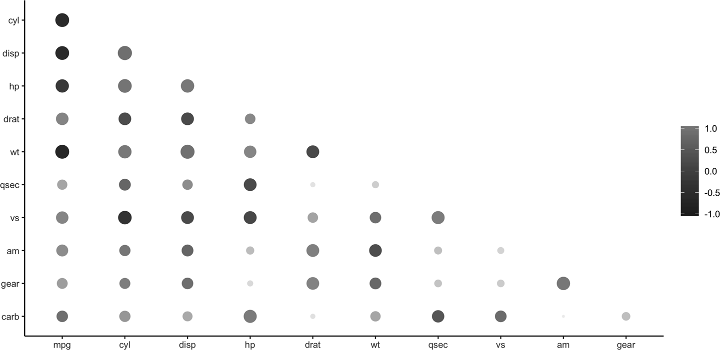
\includegraphics{figures/3_6.png}
\caption{图3-6. 使用\texttt{rplot()}可视化相关性}
\end{figure}

很容易看到哪些关系是正向的,哪些是负向的。正向关系是灰色的,负向关系是黑色的。圆圈的大小表示关系的显著程度。可视化数据的作用在于它可以让我们更加容易的理解结果。下一节会介绍这方面的内容。

\hypertarget{ux53efux89c6ux5316}{%
\subsection{可视化}\label{ux53efux89c6ux5316}}

可视化是帮助我们发现数据模式的重要工具。相对于列表,画出一个图形可以让我们更容易发现数据中的异常点。R是做数据可视化的有些工具。

R语言的绘图能力可以通过许多关注分析的程序包来扩展。不幸的是,大部分绘图的R函数都需要数据加载在本地内存中,所以使用它并不能在Spark中使用远程数据表。

然而我们还是可以使用R给Spark中的数据源做可视化。要明白其中的原理,让我们首先理解计算机是如何绘制图形的。首先,程序读入原始数据并完成一些数据转换。转换后的数据映射成一些坐标点。最后,映射出的值绘制在图中。图3-7描述了每一步。

\begin{figure}
\centering
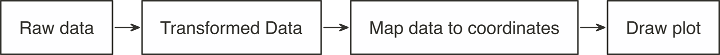
\includegraphics{figures/3_7.png}
\caption{图3-7. 一个R图形的各个阶段}
\end{figure}

可视化方法本质上与数据操作一样:让Saprk做计算,然后收集结果绘制图形。如图3-8,准备数据的繁重工作,例如按照分组或者分箱聚合数据可以在Spark中完成,而小很多的数据集可以在R中操作。R
中的绘图变成了非常基本的操作。例如,一个直方图的分箱可以在Spark中计算,而R语言不用绘制直方图,而是实现简单的柱形图绘制。R语言没有必要在计算一次分箱。

\begin{figure}
\centering
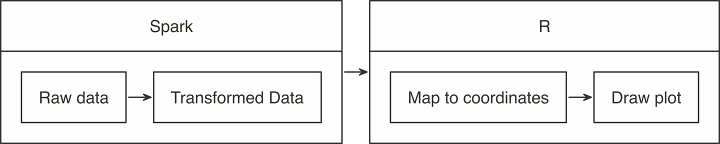
\includegraphics{figures/3_8.png}
\caption{图3-8. 使用Spark和R绘图}
\end{figure}

让我们通过\texttt{ggplot2}来应用这个概念模型。

\hypertarget{ux4f7fux7528ggplot2}{%
\subsubsection{\texorpdfstring{使用\texttt{ggplot2}}{使用ggplot2}}\label{ux4f7fux7528ggplot2}}

要使用\texttt{ggplot2}绘制柱形图,只需调用一个函数:

\begin{Shaded}
\begin{Highlighting}[]
\KeywordTok{library}\NormalTok{(ggplot2)}
\KeywordTok{ggplot}\NormalTok{(}\KeywordTok{aes}\NormalTok{(}\KeywordTok{as.factor}\NormalTok{(cyl), mpg), }\DataTypeTok{data =}\NormalTok{ mtcars) }\OperatorTok{+}\StringTok{ }\KeywordTok{geom_col}\NormalTok{()}
\end{Highlighting}
\end{Shaded}

在这个例子中,\texttt{mtcars}原始数据自动的转换成3个离散的聚合数字。然后,每个结果都映射到\texttt{x}和\texttt{y}轴。接着,画出图形。作为R用户,绘图的所有阶段都非常便捷的抽象出来。

在Spark中,有两个关键的步骤来践行``推动计算,收集数据''的理念。第一个是确保在Spark中完成转换操作。在后面的例子中,\texttt{group\_by()}和\texttt{summarise()}会在Spark中运行。第二个是数据完成转换后返回给R。确保先转换数据后返回结果的顺序。如果\texttt{collect()}先运行,R会加载Spark中的全部数据集。根据数据集规模的不同,收集全部数据会拖慢你的系统,甚至宕机。

\begin{Shaded}
\begin{Highlighting}[]
\NormalTok{car_group <-}\StringTok{ }\NormalTok{cars }\OperatorTok
\KeywordTok{group_by}\NormalTok{(cyl) }\OperatorTok
\KeywordTok{summarise}\NormalTok{(}\DataTypeTok{mpg =} \KeywordTok{sum}\NormalTok{(mpg, }\DataTypeTok{na.rm =} \OtherTok{TRUE}\NormalTok{)) }\OperatorTok
\KeywordTok{collect}\NormalTok{() }\OperatorTok
\KeywordTok{print}\NormalTok{()}
\CommentTok{# A tibble: 3 x 2}
\NormalTok{ cyl mpg}
 \OperatorTok{<}\NormalTok{dbl}\OperatorTok{>}\StringTok{ }\ErrorTok{<}\NormalTok{dbl}\OperatorTok{>}
\DecValTok{1} \DecValTok{6} \FloatTok{138.}
\DecValTok{2} \DecValTok{4} \FloatTok{293.}
\DecValTok{3} \DecValTok{8} \FloatTok{211.}
\end{Highlighting}
\end{Shaded}

在这个例子中,既然数据已经预先聚合好,并且返回给了R,只用给绘图函数传递三条记录即可:

\begin{Shaded}
\begin{Highlighting}[]
\KeywordTok{ggplot}\NormalTok{(}\KeywordTok{aes}\NormalTok{(}\KeywordTok{as.factor}\NormalTok{(cyl), mpg), }\DataTypeTok{data =}\NormalTok{ car_group) }\OperatorTok{+}\StringTok{ }\KeywordTok{geom_col}\NormalTok{(}\DataTypeTok{fill =} \StringTok{"#999999"}\NormalTok{) }\OperatorTok{+}\StringTok{ }
\StringTok{    }\KeywordTok{coord_flip}\NormalTok{()}
\end{Highlighting}
\end{Shaded}

图3-9展示了绘图结果。

\begin{figure}
\centering
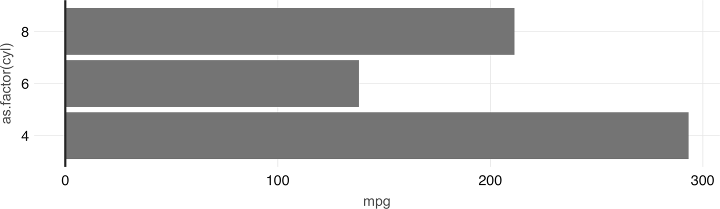
\includegraphics{figures/3_9.png}
\caption{图3-9. Spark中绘制聚合结果}
\end{figure}

绘制其它\texttt{ggplot2}可视化都可以使用这个方法。但是,这部分内容超出了本书的范畴。我们推荐你可以查阅
Winston Chang 的《R Graphics
Cookbook》,学习其它的Spark支持的可视化技术。现在,要简化可视化前的数据转换,\texttt{dbplot}程序包提供了一些立即可用的可视化方法,来自动化Spark中的聚合计算。

\hypertarget{ux4f7fux7528dbplot}{%
\subsubsection{\texorpdfstring{使用\texttt{dbplot}}{使用dbplot}}\label{ux4f7fux7528dbplot}}

\texttt{dbplot}程序包为远程数据提供了有用的绘图函数。\texttt{dbplot}中用于转换数据的代码已经完成,以便可以对应到Spark中。它会使用这些结果,通过\texttt{ggplot2}程序包创建图形,其中数据转换和绘图都是由一个函数完成的。\texttt{dbplot\_histogram()}函数可以让Spark计算分箱,并对每个分箱计数,产出一个\texttt{ggplot}对象,这个对象可以通过后续添加其他步骤进行优化。\texttt{dbplot\_histogram()}也接受\texttt{binwidth}参数来控制用于计算分箱的数据范围:

\begin{Shaded}
\begin{Highlighting}[]
\KeywordTok{library}\NormalTok{(dbplot)}
\NormalTok{cars }\OperatorTok\StringTok{ }\KeywordTok{dbplot_histogram}\NormalTok{(mpg, }\DataTypeTok{binwidth =} \DecValTok{3}\NormalTok{) }\OperatorTok{+}\StringTok{ }\KeywordTok{labs}\NormalTok{(}\DataTypeTok{title =} \StringTok{"MPG Distribution"}\NormalTok{, }\DataTypeTok{subtitle =} \StringTok{"Histogram over miles per gallon"}\NormalTok{)}
\end{Highlighting}
\end{Shaded}

图3-10给出了绘图结果。

\begin{figure}
\centering
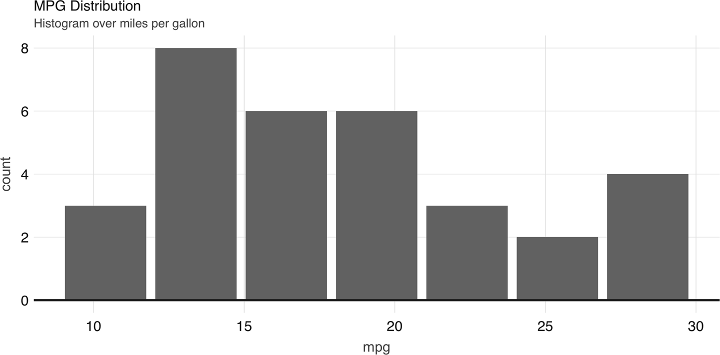
\includegraphics{figures/3_10.png}
\caption{图3-10. \texttt{dbplot}创建的直方图}
\end{figure}

直方图是分析单变量的好方法。要分析两个变量,我们经常会用到散点图或光栅图。散点图用来对比两个连续型变量的关系。例如,一个散点图会展示汽车重量和汽油消耗之间的关系。图3-11说明,汽车越重,汽油消耗越多,因为这些点几乎靠拢成一条线,从左上角下降到右下角。下面是是生成图形的代码:

\begin{Shaded}
\begin{Highlighting}[]
\KeywordTok{ggplot}\NormalTok{(}\KeywordTok{aes}\NormalTok{(mpg, wt), }\DataTypeTok{data =}\NormalTok{ mtcars) }\OperatorTok{+}\StringTok{ }\KeywordTok{geom_point}\NormalTok{()}
\end{Highlighting}
\end{Shaded}

\begin{figure}
\centering
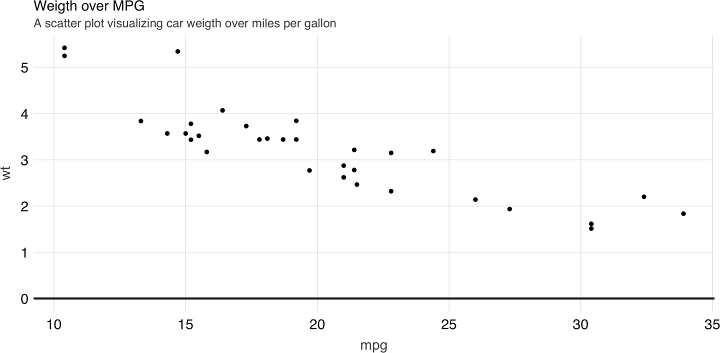
\includegraphics{figures/3_11.png}
\caption{图3-11. Spark中的散点图示例}
\end{figure}

However, for scatter plots, no amount of ``pushing the computation'' to
Spark will help with this problem because the data must be plotted in
individual dots. The best alternative is to find a plot type that
represents the x/y relationship and con‐ centration in a way that it is
easy to perceive and to ``physically'' plot. The raster plot might be
the best answer. A raster plot returns a grid of x/y positions and the
results of a given aggregation, usually represented by the color of the
square. You can use \texttt{dbplot\_raster()} to create a scatter-like
plot in Spark, while only retriev‐ ing (collecting) a small subset of
the remote dataset:

\begin{Shaded}
\begin{Highlighting}[]
\KeywordTok{dbplot_raster}\NormalTok{(cars, mpg, wt, }\DataTypeTok{resolution =} \DecValTok{16}\NormalTok{)}
\end{Highlighting}
\end{Shaded}

As shown in图3-12, the resulting plot returns a grid no bigger than 5 x
5. This limits the number of records that need to be collected into R to
25.

\begin{figure}
\centering
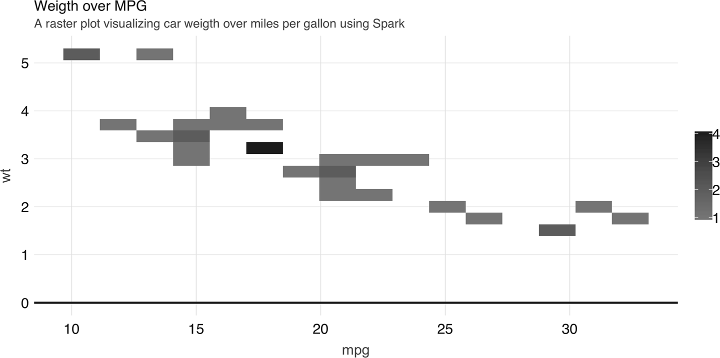
\includegraphics{figures/3_12.png}
\caption{图3-12. A raster plot using Spark}
\end{figure}

\begin{quote}
你也可以使用\texttt{dbplot}获取原始数据并用其他方式做可视化。要获取聚合结果,而不是图形,使用
\texttt{db\_compute\_bins()},\texttt{db\_compute\_count()},\texttt{db\_compute\_raster()}和\texttt{db\_compute\_boxplot()}。
\end{quote}

While visualizations are indispensable, you can complement data analysis
using stat‐ istical models to gain even deeper insights into our data.
The next section describes how we can prepare data for modeling with
Spark.

\hypertarget{ux5efaux6a21-1}{%
\subsection{建模}\label{ux5efaux6a21-1}}

下面两章完全关注建模。本章不会过多地介绍建模的细节,而是介绍如何在做数据分析的时候与模型交互。

首先,一个分析项目经过很多数据转换和模型才能找出答案。这也是为什么图3-2中的第一个数据分析图展示了一个周期,包括:可视化,数据操作和建模。我们清楚,不管是在R环境中还是使用Spark的过程中,你都不会止步于建模。

所以,理想的数据分析语言可以让你快速的在``数据操作-可视化-建模''的迭代中切换。幸运的是,这就是使用Spark和R的场景。

为了说明在Spark中迭代数据操作和建模多么简单,可以考虑下面的例子。首先我们会在所有的特征上做一个线性回归,并且预测每加仑的英里数:

\begin{Shaded}
\begin{Highlighting}[]
\NormalTok{cars }\OperatorTok
\KeywordTok{ml_linear_regression}\NormalTok{(mpg }\OperatorTok{~}\StringTok{ }\NormalTok{.) }\OperatorTok
\KeywordTok{summary}\NormalTok{()}
\NormalTok{Deviance Residuals}\OperatorTok{:}
\StringTok{ }\NormalTok{Min 1Q Median 3Q Max}
\FloatTok{-3.4506} \FloatTok{-1.6044} \FloatTok{-0.1196} \FloatTok{1.2193} \FloatTok{4.6271}
\NormalTok{Coefficients}\OperatorTok{:}
\NormalTok{(Intercept) cyl disp hp drat wt}
\FloatTok{12.30337416} \FloatTok{-0.11144048} \FloatTok{0.01333524} \FloatTok{-0.02148212} \FloatTok{0.78711097} \FloatTok{-3.71530393}
\NormalTok{ qsec vs am gear carb}
\FloatTok{0.82104075} \FloatTok{0.31776281} \FloatTok{2.52022689} \FloatTok{0.65541302} \FloatTok{-0.19941925}
\NormalTok{R}\OperatorTok{-}\NormalTok{Squared}\OperatorTok{:}\StringTok{ }\FloatTok{0.869}
\NormalTok{Root Mean Squared Error}\OperatorTok{:}\StringTok{ }\FloatTok{2.147}
\end{Highlighting}
\end{Shaded}

现在,很容易使用不同的特征做实验。我们可以简单的改变R中的公式,把\texttt{mpg\ \textasciitilde{}\ .}改成\texttt{mpg\ \textasciitilde{}\ hp\ +\ cyl},以便只使用马力和气缸作为特征:

\begin{Shaded}
\begin{Highlighting}[]
\NormalTok{cars }\OperatorTok
\KeywordTok{ml_linear_regression}\NormalTok{(mpg }\OperatorTok{~}\StringTok{ }\NormalTok{hp }\OperatorTok{+}\StringTok{ }\NormalTok{cyl) }\OperatorTok
\KeywordTok{summary}\NormalTok{()}
\NormalTok{Deviance Residuals}\OperatorTok{:}
\StringTok{ }\NormalTok{Min 1Q Median 3Q Max}
\FloatTok{-4.4948} \FloatTok{-2.4901} \FloatTok{-0.1828} \FloatTok{1.9777} \FloatTok{7.2934}
\NormalTok{Coefficients}\OperatorTok{:}
\NormalTok{(Intercept) hp cyl}
 \FloatTok{36.9083305} \FloatTok{-0.0191217} \FloatTok{-2.2646936}
\NormalTok{R}\OperatorTok{-}\NormalTok{Squared}\OperatorTok{:}\StringTok{ }\FloatTok{0.7407}
\NormalTok{Root Mean Squared Error}\OperatorTok{:}\StringTok{ }\FloatTok{3.021}
\end{Highlighting}
\end{Shaded}

另外,在不同的模型上迭代也非常容易。下面的例子把线性模型换成了广义线性模型:

\begin{Shaded}
\begin{Highlighting}[]
\NormalTok{cars }\OperatorTok
\KeywordTok{ml_generalized_linear_regression}\NormalTok{(mpg }\OperatorTok{~}\StringTok{ }\NormalTok{hp }\OperatorTok{+}\StringTok{ }\NormalTok{cyl) }\OperatorTok
\KeywordTok{summary}\NormalTok{()}
\NormalTok{Deviance Residuals}\OperatorTok{:}
\StringTok{ }\NormalTok{Min 1Q Median 3Q Max}
\FloatTok{-4.4948} \FloatTok{-2.4901} \FloatTok{-0.1828} \FloatTok{1.9777} \FloatTok{7.2934}
\NormalTok{Coefficients}\OperatorTok{:}
\NormalTok{(Intercept) hp cyl}
 \FloatTok{36.9083305} \FloatTok{-0.0191217} \FloatTok{-2.2646936}
\NormalTok{(Dispersion parameter }\ControlFlowTok{for}\NormalTok{ gaussian family taken to be }\FloatTok{10.06809}\NormalTok{)}
\NormalTok{ Null deviance}\OperatorTok{:}\StringTok{ }\FloatTok{1126.05}\NormalTok{ on }\DecValTok{31}\NormalTok{ degress of freedom}
\NormalTok{Residual deviance}\OperatorTok{:}\StringTok{ }\FloatTok{291.975}\NormalTok{ on }\DecValTok{29}\NormalTok{ degrees of freedom}
\NormalTok{AIC}\OperatorTok{:}\StringTok{ }\FloatTok{169.56}
\end{Highlighting}
\end{Shaded}

通常,在拟合模型之前,你需要使用多个\texttt{dplyr}转换来让数据适合作为模型输入。要保证模型可以尽可能的高效拟合,你应该在拟合之前,把数据集缓存起来。我们会在下面的章节看到。

\hypertarget{ux7f13ux5b58}{%
\subsubsection{缓存}\label{ux7f13ux5b58}}

本节的例子使用非常小的数据集。在实际场景中,模型会使用大规模数据集。如果数据需要预先转换,其规模会消耗Spark大量的进程开销。拟合模型之前,最好把所有转换的结果保存到一个Spark内存的新表中。

\texttt{compute()}命令会接棒一个\texttt{dplyr}命令把结果保存到Spark内存中:

\begin{Shaded}
\begin{Highlighting}[]
\NormalTok{cached_cars <-}\StringTok{ }\NormalTok{cars }\OperatorTok
\KeywordTok{mutate}\NormalTok{(}\DataTypeTok{cyl =} \KeywordTok{paste0}\NormalTok{(}\StringTok{"cyl_"}\NormalTok{, cyl)) }\OperatorTok
\KeywordTok{compute}\NormalTok{(}\StringTok{"cached_cars"}\NormalTok{)}
\NormalTok{cached_cars }\OperatorTok
\KeywordTok{ml_linear_regression}\NormalTok{(mpg }\OperatorTok{~}\StringTok{ }\NormalTok{.) }\OperatorTok
\KeywordTok{summary}\NormalTok{()}
\NormalTok{Deviance Residuals}\OperatorTok{:}
\StringTok{ }\NormalTok{Min 1Q Median 3Q Max}
\FloatTok{-3.47339} \FloatTok{-1.37936} \FloatTok{-0.06554} \FloatTok{1.05105} \FloatTok{4.39057}
\NormalTok{Coefficients}\OperatorTok{:}
\NormalTok{(Intercept) cyl_cyl_}\FloatTok{8.0}\NormalTok{ cyl_cyl_}\FloatTok{4.0}\NormalTok{ disp hp drat}
\FloatTok{16.15953652} \FloatTok{3.29774653} \FloatTok{1.66030673} \FloatTok{0.01391241} \FloatTok{-0.04612835} \FloatTok{0.02635025}
\NormalTok{ wt qsec vs am gear carb}
 \FloatTok{-3.80624757} \FloatTok{0.64695710} \FloatTok{1.74738689} \FloatTok{2.61726546} \FloatTok{0.76402917} \FloatTok{0.50935118}
\NormalTok{R}\OperatorTok{-}\NormalTok{Squared}\OperatorTok{:}\StringTok{ }\FloatTok{0.8816}
\NormalTok{Root Mean Squared Error}\OperatorTok{:}\StringTok{ }\FloatTok{2.041}
\end{Highlighting}
\end{Shaded}

由于数据可以提炼出更多的理解,更多的问题也会随之提出来。这也是为什么我们希望通过数据操作,可视化和建模,来多次迭代。每次迭代应该增量的提供数据给我们传递的含义。我们会有一个时间点,
来达到一个满意的理解水准。在这个点上,我们就可以分享分析的结果。这就是下一章节的主题。

\hypertarget{ux6c9fux901a}{%
\subsection{沟通}\label{ux6c9fux901a}}

清楚的沟通分析结果非常重要,甚至和分析工作本身一样重要?公众,同事或者利益相关者需要知道你发现了什么信息,以及发现的方法。

为了有效的沟通,我们需要使用一些途径,例如报告或者展示:这些都是可以使用R环境中的\emph{R
markdown}创建的常见输出格式。R
Markdown文档可以让你一起编写介绍性的文字和代码。不同的输出格式让R
markdown的学习和使用变得很迫切。有很多可用的输出格式,例如HTML,PDF,PowerPoint,Word,网页幻灯片,网站,书籍等等。

大部分输出可以通过R
markdown的核心程序包生成,例如\texttt{knitr}和\texttt{rmarkdown}。你可以使用其他程序包扩展R
Markdown。例如,本书就是用R
Markdown编写的,基于\texttt{bookdown}程序包提供的扩展而完成。深度了解R
Markdown的最优资源是官方书籍\footnote{Xie Allaire G (2018). R Markdown:
  The Definite Guide, 1st edition. CRC Press.}。

在R
Markdown中,一个文档可以被渲染成不同的格式。例如,你可以渲染同一份报告,通过在报告中设置不同的参数得到HTML或PDF文件。相反,许多不同类型的文档也可以渲染成同样的输出格式。例如,一个展示平台和一个报告都可以渲染成HTML格式。

使用Spark作为计算引擎,创建一个新的R Markdown报告并不难。在文件头部,R
Markdown需要一个YAML标头。第一行和最后一行是三个连续短横线(\texttt{-\/-\/-})。短横线之间的内容可以根据文档类型不同而变化。YAML标头中唯一必需的字段是\texttt{output}值。R
Markdown需要知道它要把报告渲染成哪种类型的输出。这个YAML标头叫做\emph{前辅文(frontmatter)}。前辅文后面是各种的代码,叫做\emph{代码块(code
chunks)}。这些代码块可以和介绍性文件交叉在一起。在Spark中使用R
Markdown也并没有什么特别不同的地方:只是和平时的工作一样。

由于R
Markdown文档是自含的并且是可以复现的,在润色文档之前,我们首先从Spark断开连接:

\begin{Shaded}
\begin{Highlighting}[]
\KeywordTok{spark_disconnect}\NormalTok{(sc)}
\end{Highlighting}
\end{Shaded}

下面的例子展示了创建一个完全可复现的有关Spark处理大规模数据集的报告是多么的容易。介绍性文字,代码,以及最重要的代码输出都记录在最后的HTML文件中。你可以把下面的代码复制粘贴到一个文件中,并用\emph{.Rmd}后缀保存起来,确定一个喜欢的文件名字:

\begin{verbatim}
---
title: "mtcars analysis"
output:
 html_document:
 fig_width: 6
 fig_height: 3
---
\end{verbatim}

\begin{Shaded}
\begin{Highlighting}[]
\KeywordTok{library}\NormalTok{(ggplot2)}
\NormalTok{cars }\OperatorTok
\StringTok{ }\KeywordTok{group_by}\NormalTok{(cyl) }\OperatorTok\StringTok{ }\KeywordTok{summarise}\NormalTok{(}\DataTypeTok{mpg =} \KeywordTok{mean}\NormalTok{(mpg)) }\OperatorTok
\StringTok{ }\KeywordTok{ggplot}\NormalTok{(}\KeywordTok{aes}\NormalTok{(cyl, mpg)) }\OperatorTok{+}\StringTok{ }\KeywordTok{geom_bar}\NormalTok{(}\DataTypeTok{stat=}\StringTok{"identity"}\NormalTok{)}


\CommentTok{## Model}
\NormalTok{The selected model was a simple linear regression that}
\NormalTok{uses the weight as the predictor of MPG}
\end{Highlighting}
\end{Shaded}

\begin{Shaded}
\begin{Highlighting}[]
\NormalTok{cars }\OperatorTok\StringTok{ }\KeywordTok{ml_linear_regression}\NormalTok{(wt }\OperatorTok{~}\StringTok{ }\NormalTok{mpg) }\OperatorTok\StringTok{ }\KeywordTok{summary}\NormalTok{()}
\end{Highlighting}
\end{Shaded}

要生成这个报告,用\emph{.Rmd}扩展名保存,例如\emph{report.Rmd},并且运行R中的\texttt{render()}。输出结果应该和图3-13类似。

\begin{Shaded}
\begin{Highlighting}[]
\NormalTok{rmarkdown}\OperatorTok{::}\KeywordTok{render}\NormalTok{(}\StringTok{"report.Rmd"}\NormalTok{)}
\end{Highlighting}
\end{Shaded}

\begin{figure}
\centering
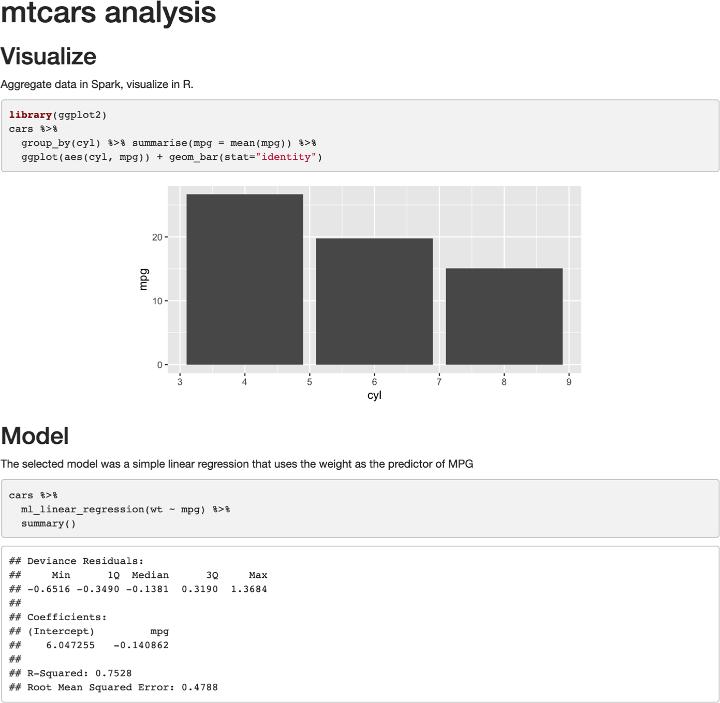
\includegraphics{figures/3_13.png}
\caption{图3-13. R Markdown HTML输出}
\end{figure}

你可以轻松的分享这个报告,并不会消耗阅读者的Spark或R资源。它是一份自含的HTML文件,任何网络浏览器都可以打开。

从一个报告中提炼出各种观点并生成不同的输出格式也很常见。格式的转换也很容易,只需改变输出选项为
\texttt{point\_presentation},\texttt{pdf\_document},\texttt{word\_document}或类似的。你甚至可以从一份报告中生成多个输出格式:

\begin{verbatim}
---
title: "mtcars analysis"
output:
 word_document: default
 pdf_document: default
 powerpoint_presentation: default
---
\end{verbatim}

最终结果是一个PowerPoint展示文档,一个Word文档和一个PDF。在原始HTML报告中展示的所有相同的信息都是通过Spark计算得出,并在R中渲染。你可能需要编辑PowerPoint模板,或者代码块的输出。

这个最小例子展示了从一种格式换成另一种格式是非常简单的。当然,R用户需要做更多的编辑工作,来保证幻灯片只包含相关信息。关键要记住,它不需要你为了从一个文档换成另一个文档,学习不同的标记语言或者代码风格。

\hypertarget{ux5c0fux7ed3-2}{%
\subsection{小结}\label{ux5c0fux7ed3-2}}

本章对R和Spark的数据分析进行了扎实的介绍。提出的许多技术看起来与只使用R而不使用Spark非常相似。这并非虎头蛇尾,而是要让已经熟悉R的用户简单的过渡到Spark的正确设计。对于不熟悉R的用户,本章还非常简要介绍R中一些最流行的(有用的)程序包。现在应该很清楚,R和Spark是一个强大的组合,一个大型计算平台,以及一个异常强大的R程序包生态系统,成为了理想的分析平台。

在使用R和Spark分析时,请记住将计算推送到Spark,并在R中收集结果。这种范式应该建立一个成功的途径,以各种输出格式分享结果,实现数据操作、可视化和沟通。
各种输出。

第4章将深入探讨如何使用大量更有趣的数据集(还有什么比约会数据集更有趣?)。你还将学习更多的技术,这些技术甚至没有在本章建模部分提及。

\begin{center}\rule{0.5\linewidth}{\linethickness}\end{center}

\hypertarget{ux7b2c4ux7ae0-ux5efaux6a21}{%
\section{第4章 建模}\label{ux7b2c4ux7ae0-ux5efaux6a21}}

\begin{quote}
I've trusted in your visions, in your prophecies, for years. ---Stannis
Baratheon
\end{quote}

在第3章中,你学到了如果在大规模数据集上利用Spark进行数据分析。在本章中,我们会详细介绍使用Spark构建预测模型的步骤。我们会研究\texttt{MLlib},Spark中支持编写高层级代码在分布式数据上进行预测建模的模块,并在特征工程和探索性数据分析的背景下使用数据操作。

我们首先结合Spark的背景以及贯穿全章的数据集,介绍建模。然后我们会展示一个有监督的学习流程,包括探索性数据分析,特征工程,和模型构建。接着,我们会使用非结构化的文本数据继续介绍无监督的主题建模示例。切记,我们的目标是介绍大规模数据集上执行数据科学任务的各种技术,而不是指导严谨一致的分析。Spark中海油许多其他的模型并不会在本章中介绍。,但是在本章的末尾,你会看到一些不错的工具,可以试试用自己的模型做实验。

手动预测数据集通常是一个合理的手段(``手动''是指人们给Spark导入数据集,使用拟合好的模型来丰富或预测取值)。这引出一个问题,我们可以把这个过程自动化为任何人都可以使用的系统吗?例如,我们如何构建一个系统可以自动的识别垃圾邮件,而不用手动分析每一个邮箱账户?第5章会介绍自动化数据分析和建模流程的工具。但是在这之前,我们首先需要知道如何``亲手''训练模型。

\hypertarget{ux6982ux8ff0-3}{%
\subsection{概述}\label{ux6982ux8ff0-3}}

R中的Spark接口提供了R用户熟悉的建模算法。例如,我们已经用过\texttt{ml\_linear\_regression(cars,\ mpg\ \textasciitilde{}\ .)},但是我们可以只用简单的运行\texttt{ml\_logistic\_regression(cars,\ am\ \textasciitilde{}\ .)}。

花些时间看看本书附录中长长的\texttt{MLlib}函数列表。简单浏览可以发现Spark支持决策树,梯度加速树,加速失效时间生产回归,保序回归,K-Means聚类,高斯混合聚类Clustering等等。

可以看到,Spark提供了大量的算法和特征转换函数。这里我们只涉及具有代表性的一些功能。完整
的预测模型概念讲解已经超出了本书的范畴,所以我们推荐阅读Hadley
Wickham和Garrett Grolemund G
(O'Reilly)的\emph{《R语言数据科学》},以及\emph{Feature Engineering and
Selection: A Practical Approach for Predictive Models}\footnote{Kuhn M,
  Johnson K (2019). Feature Engineering and Selection: A Practical
  Approach for Predictive Models. (CRC PRess.)}。本章中的一些例子和可视化也是从这些材料中引用过来(有时候会原封不动的引用)。

本章关注预测建模,Spark力求推动机器学习而非统计推断。通常机器学习更多关注预测未来而不是推断数据生产的过程\footnote{我们也承认,这里的术语对于不同的人意味着不同的理解,二者之间也是统一的。但是,本书有一定的定义。},进而用来创建自动化系统。机器学习可以分成\emph{监督式学习}(预测建模)和\emph{非监督式学习}。在监督式学习中,通过数据集(X,Y)实例,我们试着学习一个函数可以把X映射到Y。在非监督式学习中,我们只有X,而没有Y标记。所以我们会试着学习X的结构。一些实际的监督式学习的用例包括预测明天的天气,确定信用卡交易是否虚假,制度汽车保险报价。使用非监督式学习,例子包括个人照片的自动聚类,根据购买历史划分顾客,文档聚类。

\texttt{sparklyr}中的机器学习接口设计的初衷是为了最小化认知的成本,可以轻松的从本地的,基于内存的原生R工作流转向集群计算,也包括反向的转变。然而Spark生态非常丰富,CRAN上依然有大量的程序包,帮助实现一个项目中所需要的功能。而且,你也会希望利用你在R中的技能和经验保持一定的生产力。我们在第3章中也用到了这一点。记录执行计算的位置,以及集群和R进程之间的合适转换,这很重要。

本章的例子使用\emph{OkCupid}数据集\footnote{Kim AY, Escobedo-Land A
  (2015). ``OKCupid data for introductory statistics and data science
  courses.'' Journal of Statistics Education, 23(2).}。这个数据集包括来自在线约会网站的用户画像数据,以及一系列特征集合,例如性别职业等生平细节特征,还有有关个人兴趣的自由文本字段。这个数据集中有大约60,000份用户画像,可以轻松的导入目前笔记本的内存中,
算不上``大数据''。所以你可以很容易的在本地节点上运行Spark程序。

你可以下载这个数据集,代码如下:

\begin{Shaded}
\begin{Highlighting}[]
\KeywordTok{download.file}\NormalTok{(}\StringTok{"https://github.com/r-spark/okcupid/raw/master/profiles.csv.zip"}\NormalTok{, }\StringTok{"okcupid.zip"}\NormalTok{)}
\KeywordTok{unzip}\NormalTok{(}\StringTok{"okcupid.zip"}\NormalTok{, }\DataTypeTok{exdir =} \StringTok{"data"}\NormalTok{)}
\KeywordTok{unlink}\NormalTok{(}\StringTok{"okcupid.zip"}\NormalTok{)}
\end{Highlighting}
\end{Shaded}

我们不建议对这个数据集采样,因为最终模型的性能会不够好。但是,如果硬件资源受限,你还是需要进行采用,代码入下:

\begin{Shaded}
\begin{Highlighting}[]
\NormalTok{profiles <-}\StringTok{ }\KeywordTok{read.csv}\NormalTok{(}\StringTok{"data/profiles.csv"}\NormalTok{)}
\KeywordTok{write.csv}\NormalTok{(dplyr}\OperatorTok{::}\KeywordTok{sample_n}\NormalTok{(profiles, }\DecValTok{10}\OperatorTok{^}\DecValTok{3}\NormalTok{), }\StringTok{"data/profiles.csv"}\NormalTok{, }\DataTypeTok{row.names =} \OtherTok{FALSE}\NormalTok{)}
\end{Highlighting}
\end{Shaded}

\begin{quote}
本章的例子使用小型数据集,以便你可以在本地节点上运行。在实际工作中,如果你的数据集可以很轻松的导入到本地内存中,可以考虑使用一个高效的,非分布式的模型算法实现。例如你可以使用\texttt{ranger}程序包,而不是\texttt{ml\_random\_forest\_classifier()}。
\end{quote}

另外,你需要安装一些额外的程序包:

\begin{Shaded}
\begin{Highlighting}[]
\KeywordTok{install.packages}\NormalTok{(}\StringTok{"ggmosaic"}\NormalTok{)}
\KeywordTok{install.packages}\NormalTok{(}\StringTok{"forcats"}\NormalTok{)}
\KeywordTok{install.packages}\NormalTok{(}\StringTok{"FactoMineR"}\NormalTok{)}
\end{Highlighting}
\end{Shaded}

要运行示例,我们考虑以下问题:

对是否有人还在上班进行预测。也就是说,没有退休,不是学生,也不是失业的状态。

下面我们探索这个数据集。

\hypertarget{ux63a2ux7d22ux6027ux6570ux636eux5206ux6790}{%
\subsection{探索性数据分析}\label{ux63a2ux7d22ux6027ux6570ux636eux5206ux6790}}

探索性数据分析(Exploratory data
analysis,EDA),在预测建模领域中是指查看部分数据,和进行数据汇总的行为。EDA阶段的具体目的由业务问题定义,但是也有一些共通的目标:

\begin{itemize}
\tightlist
\item
  确认数据质量;确认缺失值的含义和缺失程度,根据当期条件确定统计量。
\item
  理解单变量的含义。
\item
  初步评估纳入的变量和需要的转换。
\end{itemize}

首先,连接到Spark,加载相关的库,读取数据:

\begin{Shaded}
\begin{Highlighting}[]
\KeywordTok{library}\NormalTok{(sparklyr)}
\KeywordTok{library}\NormalTok{(ggplot2)}
\KeywordTok{library}\NormalTok{(dbplot)}
\KeywordTok{library}\NormalTok{(dplyr)}
\NormalTok{sc <-}\StringTok{ }\KeywordTok{spark_connect}\NormalTok{(}\DataTypeTok{master =} \StringTok{"local"}\NormalTok{, }\DataTypeTok{version =} \StringTok{"2.3"}\NormalTok{)}
\NormalTok{okc <-}\StringTok{ }\KeywordTok{spark_read_csv}\NormalTok{(sc, }\StringTok{"data/profiles.csv"}\NormalTok{, }\DataTypeTok{escape =} \StringTok{"}\CharTok{\textbackslash{}"}\StringTok{"}\NormalTok{, }\DataTypeTok{memory =} \OtherTok{FALSE}\NormalTok{, }\DataTypeTok{options =} \KeywordTok{list}\NormalTok{(}\DataTypeTok{multiline =} \OtherTok{TRUE}\NormalTok{)) }\OperatorTok\StringTok{ }
\StringTok{    }\KeywordTok{mutate}\NormalTok{(}\DataTypeTok{height =} \KeywordTok{as.numeric}\NormalTok{(height), }\DataTypeTok{income =} \KeywordTok{ifelse}\NormalTok{(income }\OperatorTok{==}\StringTok{ "-1"}\NormalTok{, }\OtherTok{NA}\NormalTok{, }\KeywordTok{as.numeric}\NormalTok{(income))) }\OperatorTok\StringTok{ }
\StringTok{    }\KeywordTok{mutate}\NormalTok{(}\DataTypeTok{sex =} \KeywordTok{ifelse}\NormalTok{(}\KeywordTok{is.na}\NormalTok{(sex), }\StringTok{"missing"}\NormalTok{, sex)) }\OperatorTok\StringTok{ }\KeywordTok{mutate}\NormalTok{(}\DataTypeTok{drinks =} \KeywordTok{ifelse}\NormalTok{(}\KeywordTok{is.na}\NormalTok{(drinks), }
    \StringTok{"missing"}\NormalTok{, drinks)) }\OperatorTok\StringTok{ }\KeywordTok{mutate}\NormalTok{(}\DataTypeTok{drugs =} \KeywordTok{ifelse}\NormalTok{(}\KeywordTok{is.na}\NormalTok{(drugs), }\StringTok{"missing"}\NormalTok{, drugs)) }\OperatorTok\StringTok{ }
\StringTok{    }\KeywordTok{mutate}\NormalTok{(}\DataTypeTok{job =} \KeywordTok{ifelse}\NormalTok{(}\KeywordTok{is.na}\NormalTok{(job), }\StringTok{"missing"}\NormalTok{, job))}
\end{Highlighting}
\end{Shaded}

我们给定\texttt{escape\ =\ "\textbackslash{}""}和\texttt{options\ =\ list(multiline\ =\ TRUE)},接受字段中自带的引号和换行符。我们把\texttt{height}和\texttt{income}列的属性转换成数值类型,并按字符型记录缺失值。需要注意,最好尝试几次给定不同的参数,保证数据的输入是正确的。有时,即使在获取数据更多数据理解的建模阶段,你也需要回头看看这些步骤。

现在我们可以使用\texttt{glimpse()}快速查看一下数据:

\begin{Shaded}
\begin{Highlighting}[]
\KeywordTok{glimpse}\NormalTok{(okc)}
\NormalTok{Observations}\OperatorTok{:}\StringTok{ }\NormalTok{??}
\NormalTok{Variables}\OperatorTok{:}\StringTok{ }\DecValTok{31}
\NormalTok{Database}\OperatorTok{:}\StringTok{ }\NormalTok{spark_connection}
\OperatorTok{$}\StringTok{ }\NormalTok{age }\OperatorTok{<}\NormalTok{int}\OperatorTok{>}\StringTok{ }\DecValTok{22}\NormalTok{, }\DecValTok{35}\NormalTok{, }\DecValTok{38}\NormalTok{, }\DecValTok{23}\NormalTok{, }\DecValTok{29}\NormalTok{, }\DecValTok{29}\NormalTok{, }\DecValTok{32}\NormalTok{, }\DecValTok{31}\NormalTok{, }\DecValTok{24}\NormalTok{, }\DecValTok{37}\NormalTok{, 35…}
\OperatorTok{$}\StringTok{ }\NormalTok{body_type }\OperatorTok{<}\NormalTok{chr}\OperatorTok{>}\StringTok{ "a little extra"}\NormalTok{, }\StringTok{"average"}\NormalTok{, }\StringTok{"thin"}\NormalTok{, }\StringTok{"thin…}
\StringTok{$ diet <chr> "}\NormalTok{strictly anything}\StringTok{", "}\NormalTok{mostly other}\StringTok{", "}\NormalTok{anyt…}
\OperatorTok{$}\StringTok{ }\NormalTok{drinks }\OperatorTok{<}\NormalTok{chr}\OperatorTok{>}\StringTok{ "socially"}\NormalTok{, }\StringTok{"often"}\NormalTok{, }\StringTok{"socially"}\NormalTok{, }\StringTok{"socially…}
\StringTok{$ drugs <chr> "}\NormalTok{never}\StringTok{", "}\NormalTok{sometimes}\StringTok{", "}\NormalTok{missing}\StringTok{", "}\NormalTok{missing}\StringTok{"…}
\StringTok{$ education <chr> "}\NormalTok{working on college}\OperatorTok{/}\NormalTok{university}\StringTok{", "}\NormalTok{working …}
\OperatorTok{$}\StringTok{ }\NormalTok{essay0 }\OperatorTok{<}\NormalTok{chr}\OperatorTok{>}\StringTok{ "about me:<br />}\CharTok{\textbackslash{}n}\StringTok{<br />}\CharTok{\textbackslash{}n}\StringTok{i would love to …}
\StringTok{$ essay1 <chr> "}\NormalTok{currently working as an international age…}
\OperatorTok{$}\StringTok{ }\NormalTok{essay2 }\OperatorTok{<}\NormalTok{chr}\OperatorTok{>}\StringTok{ "making people laugh.<br />}\CharTok{\textbackslash{}n}\StringTok{ranting about…}
\StringTok{$ essay3 <chr> "}\NormalTok{the way i look. i am a six foot half asia…}
\OperatorTok{$}\StringTok{ }\NormalTok{essay4 }\OperatorTok{<}\NormalTok{chr}\OperatorTok{>}\StringTok{ "books:<br />}\CharTok{\textbackslash{}n}\StringTok{absurdistan, the republic, …}
\StringTok{$ essay5 <chr> "}\NormalTok{food.}\OperatorTok{<}\NormalTok{br }\OperatorTok{/}\ErrorTok{>}\NormalTok{\textbackslash{}nwater.}\OperatorTok{<}\NormalTok{br }\OperatorTok{/}\ErrorTok{>}\NormalTok{\textbackslash{}ncell phone.}\OperatorTok{<}\NormalTok{br…}
\OperatorTok{$}\StringTok{ }\NormalTok{essay6 }\OperatorTok{<}\NormalTok{chr}\OperatorTok{>}\StringTok{ "duality and humorous things"}\NormalTok{, }\StringTok{"missing"}\NormalTok{, …}
\OperatorTok{$}\StringTok{ }\NormalTok{essay7 }\OperatorTok{<}\NormalTok{chr}\OperatorTok{>}\StringTok{ "trying to find someone to hang out with. …}
\StringTok{$ essay8 <chr> "}\NormalTok{i am new to california and looking }\ControlFlowTok{for}\NormalTok{ so…}
\OperatorTok{$}\StringTok{ }\NormalTok{essay9 }\OperatorTok{<}\NormalTok{chr}\OperatorTok{>}\StringTok{ "you want to be swept off your feet!<br />…}
\StringTok{$ ethnicity <chr> "}\NormalTok{asian, white}\StringTok{", "}\NormalTok{white}\StringTok{", "}\NormalTok{missing}\StringTok{", "}\NormalTok{white…}
\OperatorTok{$}\StringTok{ }\NormalTok{height }\OperatorTok{<}\NormalTok{dbl}\OperatorTok{>}\StringTok{ }\DecValTok{75}\NormalTok{, }\DecValTok{70}\NormalTok{, }\DecValTok{68}\NormalTok{, }\DecValTok{71}\NormalTok{, }\DecValTok{66}\NormalTok{, }\DecValTok{67}\NormalTok{, }\DecValTok{65}\NormalTok{, }\DecValTok{65}\NormalTok{, }\DecValTok{67}\NormalTok{, }\DecValTok{65}\NormalTok{, 70…}
\OperatorTok{$}\StringTok{ }\NormalTok{income }\OperatorTok{<}\NormalTok{dbl}\OperatorTok{>}\StringTok{ }\OtherTok{NaN}\NormalTok{, }\DecValTok{80000}\NormalTok{, }\OtherTok{NaN}\NormalTok{, }\DecValTok{20000}\NormalTok{, }\OtherTok{NaN}\NormalTok{, }\OtherTok{NaN}\NormalTok{, }\OtherTok{NaN}\NormalTok{, NaN…}
\OperatorTok{$}\StringTok{ }\NormalTok{job }\OperatorTok{<}\NormalTok{chr}\OperatorTok{>}\StringTok{ "transportation"}\NormalTok{, }\StringTok{"hospitality / travel"}\NormalTok{, …}
\OperatorTok{$}\StringTok{ }\NormalTok{last_online }\OperatorTok{<}\NormalTok{chr}\OperatorTok{>}\StringTok{ "2012-06-28-20-30"}\NormalTok{, }\StringTok{"2012-06-29-21-41"}\NormalTok{, }\StringTok{"2…}
\StringTok{$ location <chr> "}\NormalTok{south san francisco, california}\StringTok{", "}\NormalTok{oaklan…}
\OperatorTok{$}\StringTok{ }\NormalTok{offspring }\OperatorTok{<}\NormalTok{chr}\OperatorTok{>}\StringTok{ "doesn&rsquo;t have kids, but might want t…}
\StringTok{$ orientation <chr> "}\NormalTok{straight}\StringTok{", "}\NormalTok{straight}\StringTok{", "}\NormalTok{straight}\StringTok{", "}\NormalTok{strai…}
\OperatorTok{$}\StringTok{ }\NormalTok{pets }\OperatorTok{<}\NormalTok{chr}\OperatorTok{>}\StringTok{ "likes dogs and likes cats"}\NormalTok{, }\StringTok{"likes dogs a…}
\StringTok{$ religion <chr> "}\NormalTok{agnosticism and very serious about it}\StringTok{", "}\NormalTok{…}
\OperatorTok{$}\StringTok{ }\NormalTok{sex }\OperatorTok{<}\NormalTok{chr}\OperatorTok{>}\StringTok{ "m"}\NormalTok{, }\StringTok{"m"}\NormalTok{, }\StringTok{"m"}\NormalTok{, }\StringTok{"m"}\NormalTok{, }\StringTok{"m"}\NormalTok{, }\StringTok{"m"}\NormalTok{, }\StringTok{"f"}\NormalTok{, }\StringTok{"f"}\NormalTok{, }\StringTok{"f…}
\StringTok{$ sign <chr> "}\NormalTok{gemini}\StringTok{", "}\NormalTok{cancer}\StringTok{", "}\NormalTok{pisces but it doesn}\OperatorTok{&}\NormalTok{r…}
\OperatorTok{$}\StringTok{ }\NormalTok{smokes }\OperatorTok{<}\NormalTok{chr}\OperatorTok{>}\StringTok{ "sometimes"}\NormalTok{, }\StringTok{"no"}\NormalTok{, }\StringTok{"no"}\NormalTok{, }\StringTok{"no"}\NormalTok{, }\StringTok{"no"}\NormalTok{, }\StringTok{"no"}\NormalTok{,…}
\OperatorTok{$}\StringTok{ }\NormalTok{speaks }\OperatorTok{<}\NormalTok{chr}\OperatorTok{>}\StringTok{ "english"}\NormalTok{, }\StringTok{"english (fluently), spanish (p…}
\StringTok{$ status <chr> "}\NormalTok{single}\StringTok{", "}\NormalTok{single}\StringTok{", "}\NormalTok{available}\StringTok{", "}\NormalTok{single}\StringTok{",…}
\end{Highlighting}
\end{Shaded}

我们添加一个响应变量作为一列,查看它的分布:

\begin{Shaded}
\begin{Highlighting}[]
\NormalTok{okc <-}\StringTok{ }\NormalTok{okc }\OperatorTok
\KeywordTok{mutate}\NormalTok{(}
\DataTypeTok{not_working =} \KeywordTok{ifelse}\NormalTok{(job }\OperatorTok\StringTok{ }\KeywordTok{c}\NormalTok{(}\StringTok{"student"}\NormalTok{, }\StringTok{"unemployed"}\NormalTok{, }\StringTok{"retired"}\NormalTok{), }\DecValTok{1}\NormalTok{ , }\DecValTok{0}\NormalTok{) )}
\NormalTok{okc }\OperatorTok
\KeywordTok{group_by}\NormalTok{(not_working) }\OperatorTok
\KeywordTok{tally}\NormalTok{()}
\CommentTok{# Source: spark<?> [?? x 2]}
\NormalTok{ not_working n}
 \OperatorTok{<}\NormalTok{dbl}\OperatorTok{>}\StringTok{ }\ErrorTok{<}\NormalTok{dbl}\OperatorTok{>}
\DecValTok{1} \DecValTok{0} \DecValTok{54541}
\DecValTok{2} \DecValTok{1} \DecValTok{5405}
\end{Highlighting}
\end{Shaded}

继续讲解之前,让我们先把数据分成训练集和测试集,并把测试集放在一边。事实上,这是很关键的一步,因为我们希望有一个例外的集合,可以在建模过程结束的时候用来评估模型性能。如果我们在EDA阶段囊括了所有的数据,测试集中的信息会``泄露''到可视化和汇总统计中,让我们的模型构建带有某种偏置。即便一个学习算法没有直接使用这个数据,也会发生这种情况。这会降低性能评估的可信度。我们可以简单的使用\texttt{sdf\_random\_split()}函数分割数据集:

\begin{Shaded}
\begin{Highlighting}[]
\NormalTok{data_splits <-}\StringTok{ }\KeywordTok{sdf_random_split}\NormalTok{(okc, }\DataTypeTok{training =} \FloatTok{0.8}\NormalTok{, }\DataTypeTok{testing =} \FloatTok{0.2}\NormalTok{, }\DataTypeTok{seed =} \DecValTok{42}\NormalTok{)}
\NormalTok{okc_train <-}\StringTok{ }\NormalTok{data_splits}\OperatorTok{$}\NormalTok{training}
\NormalTok{okc_test <-}\StringTok{ }\NormalTok{data_splits}\OperatorTok{$}\NormalTok{testing}
\end{Highlighting}
\end{Shaded}

我们可以快速的查看响应变量的分布:

\begin{Shaded}
\begin{Highlighting}[]
\NormalTok{okc_train }\OperatorTok
\KeywordTok{group_by}\NormalTok{(not_working) }\OperatorTok
\KeywordTok{tally}\NormalTok{() }\OperatorTok
\KeywordTok{mutate}\NormalTok{(}\DataTypeTok{frac =}\NormalTok{ n }\OperatorTok{/}\StringTok{ }\KeywordTok{sum}\NormalTok{(n))}
\CommentTok{# Source: spark<?> [?? x 3]}
\NormalTok{ not_working n frac}
 \OperatorTok{<}\NormalTok{dbl}\OperatorTok{>}\StringTok{ }\ErrorTok{<}\NormalTok{dbl}\OperatorTok{>}\StringTok{ }\ErrorTok{<}\NormalTok{dbl}\OperatorTok{>}
\DecValTok{1} \DecValTok{0} \DecValTok{43785} \FloatTok{0.910}
\DecValTok{2} \DecValTok{1} \DecValTok{4317} \FloatTok{0.0897}
\end{Highlighting}
\end{Shaded}

使用\texttt{sdf\_describe()}函数,我们可以获取具体列的数值统计信息:

\begin{Shaded}
\begin{Highlighting}[]
\KeywordTok{sdf_describe}\NormalTok{(okc_train, }\DataTypeTok{cols =} \KeywordTok{c}\NormalTok{(}\StringTok{"age"}\NormalTok{, }\StringTok{"income"}\NormalTok{))}
\CommentTok{# Source: spark<?> [?? x 3]}
\NormalTok{ summary age income}
 \OperatorTok{<}\NormalTok{chr}\OperatorTok{>}\StringTok{ }\ErrorTok{<}\NormalTok{chr}\OperatorTok{>}\StringTok{ }\ErrorTok{<}\NormalTok{chr}\OperatorTok{>}
\DecValTok{1}\NormalTok{ count }\DecValTok{48102} \DecValTok{9193}
\DecValTok{2}\NormalTok{ mean }\FloatTok{32.336534863415245} \FloatTok{104968.99815076689}
\DecValTok{3}\NormalTok{ stddev }\FloatTok{9.43908920033797} \FloatTok{202235.2291773537}
\DecValTok{4}\NormalTok{ min }\DecValTok{18} \FloatTok{20000.0}
\DecValTok{5}\NormalTok{ max }\DecValTok{110} \FloatTok{1000000.0}
\end{Highlighting}
\end{Shaded}

正如我们在第3章看到的,我们也可以使用\texttt{dbplot}程序包绘制这些变量的分布。在图4-1中,我们展示了一个年龄变量的分布直方图,其通过以下代码生成:

\begin{Shaded}
\begin{Highlighting}[]
\KeywordTok{dbplot_histogram}\NormalTok{(okc_train, age)}
\end{Highlighting}
\end{Shaded}

\begin{figure}
\centering
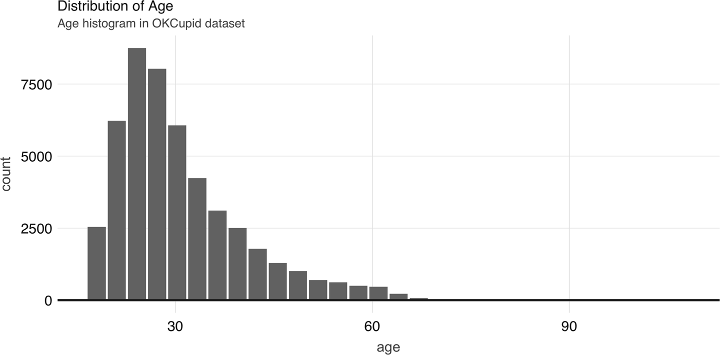
\includegraphics{figures/4_1.png}
\caption{图4-1. 年龄分布}
\end{figure}

一般的EDA操作是要查看响应变量个各个预测变量之间的关系。通常,你可能有些先验知识理解这些关系的含义,所以这些知识可以用在数据质量的检查。而且,一些异常的趋势可以展示变量的交互,你也可能把这些交互信息建模到模型中。作为一个例子,我们可以探索\texttt{religion}变量:

\begin{Shaded}
\begin{Highlighting}[]
\NormalTok{prop_data <-}\StringTok{ }\NormalTok{okc_train }\OperatorTok
\KeywordTok{mutate}\NormalTok{(}\DataTypeTok{religion =} \KeywordTok{regexp_extract}\NormalTok{(religion, }\StringTok{"^}\CharTok{\textbackslash{}\textbackslash{}\textbackslash{}\textbackslash{}}\StringTok{w+"}\NormalTok{, }\DecValTok{0}\NormalTok{)) }\OperatorTok
\KeywordTok{group_by}\NormalTok{(religion, not_working) }\OperatorTok
\KeywordTok{tally}\NormalTok{() }\OperatorTok
\KeywordTok{group_by}\NormalTok{(religion) }\OperatorTok
\KeywordTok{summarise}\NormalTok{(}
\DataTypeTok{count =} \KeywordTok{sum}\NormalTok{(n),}
\DataTypeTok{prop =} \KeywordTok{sum}\NormalTok{(not_working }\OperatorTok{*}\StringTok{ }\NormalTok{n) }\OperatorTok{/}\StringTok{ }\KeywordTok{sum}\NormalTok{(n) ) }\OperatorTok
\KeywordTok{mutate}\NormalTok{(}\DataTypeTok{se =} \KeywordTok{sqrt}\NormalTok{(prop }\OperatorTok{*}\StringTok{ }\NormalTok{(}\DecValTok{1} \OperatorTok{-}\StringTok{ }\NormalTok{prop) }\OperatorTok{/}\StringTok{ }\NormalTok{count)) }\OperatorTok
\KeywordTok{collect}\NormalTok{()}
\NormalTok{prop_data}
\CommentTok{# A tibble: 10 x 4}
\NormalTok{ religion count prop se}
 \OperatorTok{<}\NormalTok{chr}\OperatorTok{>}\StringTok{ }\ErrorTok{<}\NormalTok{dbl}\OperatorTok{>}\StringTok{ }\ErrorTok{<}\NormalTok{dbl}\OperatorTok{>}\StringTok{ }\ErrorTok{<}\NormalTok{dbl}\OperatorTok{>}
\StringTok{ }\DecValTok{1}\NormalTok{ judaism }\DecValTok{2520} \FloatTok{0.0794} \FloatTok{0.00539}
 \DecValTok{2}\NormalTok{ atheism }\DecValTok{5624} \FloatTok{0.118} \FloatTok{0.00436}
 \DecValTok{3}\NormalTok{ christianity }\DecValTok{4671} \FloatTok{0.120} \FloatTok{0.00480}
 \DecValTok{4}\NormalTok{ hinduism }\DecValTok{358} \FloatTok{0.101} \FloatTok{0.0159}
 \DecValTok{5}\NormalTok{ islam }\DecValTok{115} \FloatTok{0.191} \FloatTok{0.0367}
 \DecValTok{6}\NormalTok{ agnosticism }\DecValTok{7078} \FloatTok{0.0958} \FloatTok{0.00346}
 \DecValTok{7}\NormalTok{ other }\DecValTok{6240} \FloatTok{0.0841} \FloatTok{0.00346}
 \DecValTok{8}\NormalTok{ missing }\DecValTok{16152} \FloatTok{0.0719} \FloatTok{0.002}
 \DecValTok{9}\NormalTok{ buddhism }\DecValTok{1575} \FloatTok{0.0851} \FloatTok{0.007}
\DecValTok{10}\NormalTok{ catholicism }\DecValTok{3769} \FloatTok{0.0886} \FloatTok{0.00458}
\end{Highlighting}
\end{Shaded}

注意\texttt{prop\_data}是一个小型的数据框,它通过R进程导入到内存中,我们可以利用\texttt{ggplot2}创建一个丰富的可视化结果(见图4-2):

\begin{Shaded}
\begin{Highlighting}[]
\NormalTok{prop_data }\OperatorTok\StringTok{ }\KeywordTok{ggplot}\NormalTok{(}\KeywordTok{aes}\NormalTok{(}\DataTypeTok{x =}\NormalTok{ religion, }\DataTypeTok{y =}\NormalTok{ prop)) }\OperatorTok{+}\StringTok{ }\KeywordTok{geom_point}\NormalTok{(}\DataTypeTok{size =} \DecValTok{2}\NormalTok{) }\OperatorTok{+}\StringTok{ }\KeywordTok{geom_errorbar}\NormalTok{(}\KeywordTok{aes}\NormalTok{(}\DataTypeTok{ymin =}\NormalTok{ prop }\OperatorTok{-}\StringTok{ }
\StringTok{    }\FloatTok{1.96} \OperatorTok{*}\StringTok{ }\NormalTok{se, }\DataTypeTok{ymax =}\NormalTok{ prop }\OperatorTok{+}\StringTok{ }\FloatTok{1.96} \OperatorTok{*}\StringTok{ }\NormalTok{se), }\DataTypeTok{width =} \FloatTok{0.1}\NormalTok{) }\OperatorTok{+}\StringTok{ }\KeywordTok{geom_hline}\NormalTok{(}\DataTypeTok{yintercept =} \KeywordTok{sum}\NormalTok{(prop_data}\OperatorTok{$}\NormalTok{prop }\OperatorTok{*}\StringTok{ }
\StringTok{    }\NormalTok{prop_data}\OperatorTok{$}\NormalTok{count)}\OperatorTok{/}\KeywordTok{sum}\NormalTok{(prop_data}\OperatorTok{$}\NormalTok{count))}
\end{Highlighting}
\end{Shaded}

\begin{figure}
\centering
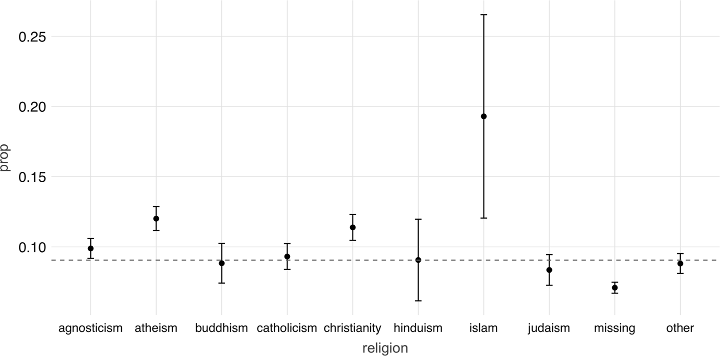
\includegraphics{figures/4_2.png}
\caption{图4-2. 当期失业人群按地区占比}
\end{figure}

然后,我们看一下两个预测变量之间的关系:饮酒和毒品。我们希望它们之间有某种相关性。你可以通过\texttt{sdf\_crosstab()}计算出一个列联表:

\begin{Shaded}
\begin{Highlighting}[]
\NormalTok{contingency_tbl <-}\StringTok{ }\NormalTok{okc_train }\OperatorTok
\KeywordTok{sdf_crosstab}\NormalTok{(}\StringTok{"drinks"}\NormalTok{, }\StringTok{"drugs"}\NormalTok{) }\OperatorTok
\KeywordTok{collect}\NormalTok{()}
\NormalTok{contingency_tbl}
\CommentTok{# A tibble: 7 x 5}
\NormalTok{ drinks_drugs missing never often sometimes}
 \OperatorTok{<}\NormalTok{chr}\OperatorTok{>}\StringTok{ }\ErrorTok{<}\NormalTok{dbl}\OperatorTok{>}\StringTok{ }\ErrorTok{<}\NormalTok{dbl}\OperatorTok{>}\StringTok{ }\ErrorTok{<}\NormalTok{dbl}\OperatorTok{>}\StringTok{ }\ErrorTok{<}\NormalTok{dbl}\OperatorTok{>}
\DecValTok{1}\NormalTok{ very often }\DecValTok{54} \DecValTok{144} \DecValTok{44} \DecValTok{137}
\DecValTok{2}\NormalTok{ socially }\DecValTok{8221} \DecValTok{21066} \DecValTok{126} \DecValTok{4106}
\DecValTok{3}\NormalTok{ not at all }\DecValTok{146} \DecValTok{2371} \DecValTok{15} \DecValTok{109}
\DecValTok{4}\NormalTok{ desperately }\DecValTok{72} \DecValTok{89} \DecValTok{23} \DecValTok{74}
\DecValTok{5}\NormalTok{ often }\DecValTok{1049} \DecValTok{1718} \DecValTok{69} \DecValTok{1271}
\DecValTok{6}\NormalTok{ missing }\DecValTok{1121} \DecValTok{1226} \DecValTok{10} \DecValTok{59}
\DecValTok{7}\NormalTok{ rarely }\DecValTok{613} \DecValTok{3689} \DecValTok{35} \DecValTok{445}
\end{Highlighting}
\end{Shaded}

我们可以使用一个马赛克图,可视化这个列联表(见图4-3):

\begin{Shaded}
\begin{Highlighting}[]
\KeywordTok{library}\NormalTok{(ggmosaic)}
\KeywordTok{library}\NormalTok{(forcats)}
\KeywordTok{library}\NormalTok{(tidyr)}
\NormalTok{contingency_tbl }\OperatorTok\StringTok{ }\KeywordTok{rename}\NormalTok{(}\DataTypeTok{drinks =}\NormalTok{ drinks_drugs) }\OperatorTok\StringTok{ }\KeywordTok{gather}\NormalTok{(}\StringTok{"drugs"}\NormalTok{, }\StringTok{"count"}\NormalTok{, missing}\OperatorTok{:}\NormalTok{sometimes) }\OperatorTok\StringTok{ }
\StringTok{    }\KeywordTok{mutate}\NormalTok{(}\DataTypeTok{drinks =} \KeywordTok{as_factor}\NormalTok{(drinks) }\OperatorTok\StringTok{ }\KeywordTok{fct_relevel}\NormalTok{(}\StringTok{"missing"}\NormalTok{, }\StringTok{"not at all"}\NormalTok{, }\StringTok{"rarely"}\NormalTok{, }
        \StringTok{"socially"}\NormalTok{, }\StringTok{"very often"}\NormalTok{, }\StringTok{"desperately"}\NormalTok{), }\DataTypeTok{drugs =} \KeywordTok{as_factor}\NormalTok{(drugs) }\OperatorTok\StringTok{ }\KeywordTok{fct_relevel}\NormalTok{(}\StringTok{"missing"}\NormalTok{, }
        \StringTok{"never"}\NormalTok{, }\StringTok{"sometimes"}\NormalTok{, }\StringTok{"often"}\NormalTok{)) }\OperatorTok\StringTok{ }\KeywordTok{ggplot}\NormalTok{() }\OperatorTok{+}\StringTok{ }\KeywordTok{geom_mosaic}\NormalTok{(}\KeywordTok{aes}\NormalTok{(}\DataTypeTok{x =} \KeywordTok{product}\NormalTok{(drinks, }
\NormalTok{    drugs), }\DataTypeTok{fill =}\NormalTok{ drinks, }\DataTypeTok{weight =}\NormalTok{ count))}
\end{Highlighting}
\end{Shaded}

\begin{figure}
\centering
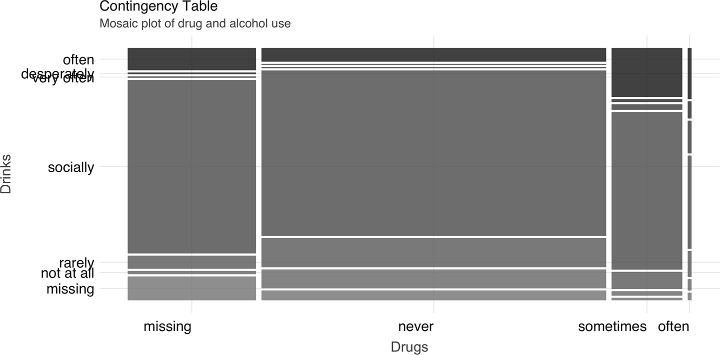
\includegraphics{figures/4_3.png}
\caption{图4-3. 毒品和酒精使用的马赛克图}
\end{figure}

要进一步探索这两个变量之间的关系,我们可以使用\texttt{FactoMineR}程序包进行对应分析\footnote{Greenacre
  M (2017). Correspondence analysis in practice. Chapman and Hall/CRC.}。这项技术可以通过把每个因子映射到平面上的一个点,让我们刻画高维因子水平之间的关系。首先,我们使用\texttt{FactoMineR::CA()}获取映射,代码如下:

\begin{Shaded}
\begin{Highlighting}[]
\NormalTok{dd_obj <-}\StringTok{ }\NormalTok{contingency_tbl }\OperatorTok\StringTok{ }\NormalTok{tibble}\OperatorTok{::}\KeywordTok{column_to_rownames}\NormalTok{(}\DataTypeTok{var =} \StringTok{"drinks_drugs"}\NormalTok{) }\OperatorTok\StringTok{ }
\StringTok{    }\NormalTok{FactoMineR}\OperatorTok{::}\KeywordTok{CA}\NormalTok{(}\DataTypeTok{graph =} \OtherTok{FALSE}\NormalTok{)}
\end{Highlighting}
\end{Shaded}

然后,我们使用\texttt{ggplot}绘制结果,如图4-4所示:

\begin{Shaded}
\begin{Highlighting}[]
\NormalTok{dd_drugs <-}\StringTok{ }\NormalTok{dd_obj}\OperatorTok{$}\NormalTok{row}\OperatorTok{$}\NormalTok{coord }\OperatorTok\StringTok{ }\KeywordTok{as.data.frame}\NormalTok{() }\OperatorTok\StringTok{ }\KeywordTok{mutate}\NormalTok{(}\DataTypeTok{label =} \KeywordTok{gsub}\NormalTok{(}\StringTok{"_"}\NormalTok{, }\StringTok{" "}\NormalTok{, }
    \KeywordTok{rownames}\NormalTok{(dd_obj}\OperatorTok{$}\NormalTok{row}\OperatorTok{$}\NormalTok{coord)), }\DataTypeTok{Variable =} \StringTok{"Drugs"}\NormalTok{)}
\NormalTok{dd_drinks <-}\StringTok{ }\NormalTok{dd_obj}\OperatorTok{$}\NormalTok{col}\OperatorTok{$}\NormalTok{coord }\OperatorTok\StringTok{ }\KeywordTok{as.data.frame}\NormalTok{() }\OperatorTok\StringTok{ }\KeywordTok{mutate}\NormalTok{(}\DataTypeTok{label =} \KeywordTok{gsub}\NormalTok{(}\StringTok{"_"}\NormalTok{, }\StringTok{" "}\NormalTok{, }
    \KeywordTok{rownames}\NormalTok{(dd_obj}\OperatorTok{$}\NormalTok{col}\OperatorTok{$}\NormalTok{coord)), }\DataTypeTok{Variable =} \StringTok{"Alcohol"}\NormalTok{)}
\NormalTok{ca_coord <-}\StringTok{ }\KeywordTok{rbind}\NormalTok{(dd_drugs, dd_drinks)}
\KeywordTok{ggplot}\NormalTok{(ca_coord, }\KeywordTok{aes}\NormalTok{(}\DataTypeTok{x =} \StringTok{`}\DataTypeTok{Dim 1}\StringTok{`}\NormalTok{, }\DataTypeTok{y =} \StringTok{`}\DataTypeTok{Dim 2}\StringTok{`}\NormalTok{, }\DataTypeTok{col =}\NormalTok{ Variable)) }\OperatorTok{+}\StringTok{ }\KeywordTok{geom_vline}\NormalTok{(}\DataTypeTok{xintercept =} \DecValTok{0}\NormalTok{) }\OperatorTok{+}\StringTok{ }
\StringTok{    }\KeywordTok{geom_hline}\NormalTok{(}\DataTypeTok{yintercept =} \DecValTok{0}\NormalTok{) }\OperatorTok{+}\StringTok{ }\KeywordTok{geom_text}\NormalTok{(}\KeywordTok{aes}\NormalTok{(}\DataTypeTok{label =}\NormalTok{ label)) }\OperatorTok{+}\StringTok{ }\KeywordTok{coord_equal}\NormalTok{()}
\end{Highlighting}
\end{Shaded}

\begin{figure}
\centering
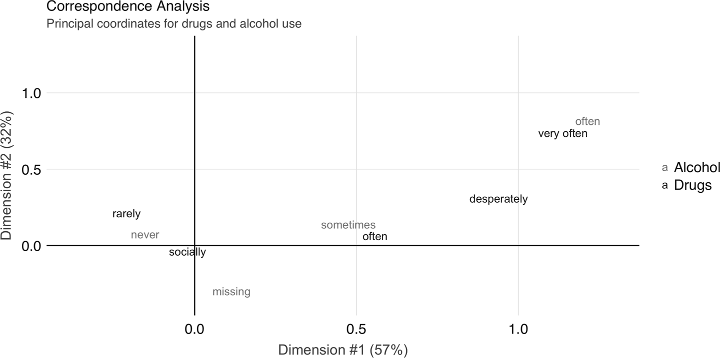
\includegraphics{figures/4_4.png}
\caption{图4-4. 毒品和酒精使用的对应分析主坐标}
\end{figure}

在图4-4中,我们看到对应分析流程把因子转换成名为\emph{主坐标}的变量,它对应因子的坐标轴并表示列联表包含了多少信息。例如,我们可以把``drinking
often''和``using drugs very often''之间的距离看成是指示性关联。

这是有关EDA的全部介绍。下面让我们介绍特征工程。

\hypertarget{ux7279ux5f81ux5de5ux7a0b}{%
\subsection{特征工程}\label{ux7279ux5f81ux5de5ux7a0b}}

特征工程实践包括数据转换,以便增加模型性能。这些实践具体指,数值的中心化和缩放,字符的操作以便获取有意义的变量等。它也包括变量选取------选择哪些预测因素用到模型中。

在图4-1中,我们看到\texttt{age}变量的取值范围是18到60以上。一些算法,特别是神经网络在归一化输入,维持相同的数据规模情况下训练的更快。现在让我们通过移除平均值和缩放单位方差,归一化\texttt{age}变量。首先计算平均值和标准差:

\begin{Shaded}
\begin{Highlighting}[]
\NormalTok{scale_values <-}\StringTok{ }\NormalTok{okc_train }\OperatorTok
\KeywordTok{summarise}\NormalTok{(}
\DataTypeTok{mean_age =} \KeywordTok{mean}\NormalTok{(age),}
\DataTypeTok{sd_age =} \KeywordTok{sd}\NormalTok{(age) ) }\OperatorTok
\KeywordTok{collect}\NormalTok{()}
\NormalTok{scale_values}
\CommentTok{# A tibble: 1 x 2}
\NormalTok{ mean_age sd_age}
 \OperatorTok{<}\NormalTok{dbl}\OperatorTok{>}\StringTok{ }\ErrorTok{<}\NormalTok{dbl}\OperatorTok{>}
\DecValTok{1} \FloatTok{32.3} \FloatTok{9.44}
\end{Highlighting}
\end{Shaded}

然后,我们使用这些信息转换数据集:

\begin{Shaded}
\begin{Highlighting}[]
\NormalTok{okc_train <-}\StringTok{ }\NormalTok{okc_train }\OperatorTok\StringTok{ }\KeywordTok{mutate}\NormalTok{(}\DataTypeTok{scaled_age =}\NormalTok{ (age }\OperatorTok{-}\StringTok{ }\OperatorTok{!!}\NormalTok{scale_values}\OperatorTok{$}\NormalTok{mean_age)}\OperatorTok{/!!}\NormalTok{scale_values}\OperatorTok{$}\NormalTok{sd_age)}
\KeywordTok{dbplot_histogram}\NormalTok{(okc_train, scaled_age)}
\end{Highlighting}
\end{Shaded}

在图4-5中,我们看到缩放后的\texttt{age}变量取值位于零附近。下面我们讨论其他类型的转换,但是在做特征工程的时候,你可能会希望对所有模型中用到的数值变量进行归一化。
Feature Engineering \textbar{} 63

\begin{figure}
\centering
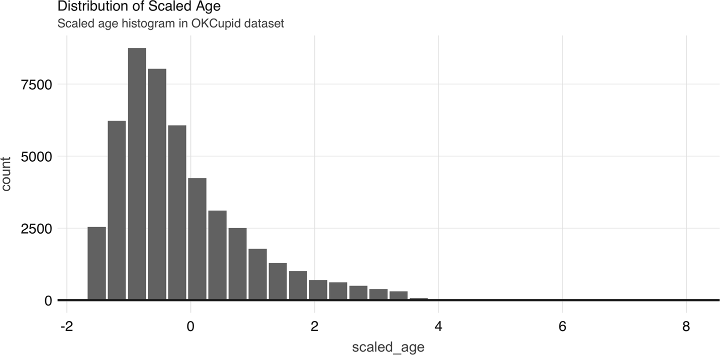
\includegraphics{figures/4_5.png}
\caption{图4-5. 缩放后\texttt{age}变量的分布}
\end{figure}

由于一些特征会被多次选取,换句话说,一个人可能对一个变量关联多个选择,我们需要在构建有意义的模型前做些处理。例如,如果我们看一下\texttt{ethnicity}列,可以发现有许多组合:

\begin{Shaded}
\begin{Highlighting}[]
\NormalTok{okc_train }\OperatorTok
\KeywordTok{group_by}\NormalTok{(ethnicity) }\OperatorTok
\KeywordTok{tally}\NormalTok{()}
\CommentTok{# Source: spark<?> [?? x 2]}
\NormalTok{ ethnicity n}
 \OperatorTok{<}\NormalTok{chr}\OperatorTok{>}\StringTok{ }\ErrorTok{<}\NormalTok{dbl}\OperatorTok{>}
\StringTok{ }\DecValTok{1}\NormalTok{ hispanic }\OperatorTok{/}\StringTok{ }\NormalTok{latin, white }\DecValTok{1051}
 \DecValTok{2}\NormalTok{ black, pacific islander, hispanic }\OperatorTok{/}\StringTok{ }\NormalTok{latin }\DecValTok{2}
 \DecValTok{3}\NormalTok{ asian, black, pacific islander }\DecValTok{5}
 \DecValTok{4}\NormalTok{ black, native american, white }\DecValTok{91}
 \DecValTok{5}\NormalTok{ middle eastern, white, other }\DecValTok{34}
 \DecValTok{6}\NormalTok{ asian, other }\DecValTok{78}
 \DecValTok{7}\NormalTok{ asian, black, white }\DecValTok{12}
 \DecValTok{8}\NormalTok{ asian, hispanic }\OperatorTok{/}\StringTok{ }\NormalTok{latin, white, other }\DecValTok{7}
 \DecValTok{9}\NormalTok{ middle eastern, pacific islander }\DecValTok{1}
\DecValTok{10}\NormalTok{ indian, hispanic }\OperatorTok{/}\StringTok{ }\NormalTok{latin }\DecValTok{5}
\CommentTok{# … with more rows}
\end{Highlighting}
\end{Shaded}

一种处理方式是把种族的每一种组合都看成是一个独立的水平,但是这会导致生成大量的水平,这会给许多算法带来问题。为了更好的编码这些信息,我们可以为每个种族创建哑变量,代码如下:

\begin{Shaded}
\begin{Highlighting}[]
\NormalTok{ethnicities <-}\StringTok{ }\KeywordTok{c}\NormalTok{(}\StringTok{"asian"}\NormalTok{, }\StringTok{"middle eastern"}\NormalTok{, }\StringTok{"black"}\NormalTok{, }\StringTok{"native american"}\NormalTok{, }\StringTok{"indian"}\NormalTok{,}
\StringTok{"pacific islander"}\NormalTok{, }\StringTok{"hispanic / latin"}\NormalTok{, }\StringTok{"white"}\NormalTok{, }\StringTok{"other"}\NormalTok{)}
\NormalTok{ethnicity_vars <-}\StringTok{ }\NormalTok{ethnicities }\OperatorTok
\NormalTok{purrr}\OperatorTok{::}\KeywordTok{map}\NormalTok{(}\OperatorTok{~}\StringTok{ }\KeywordTok{expr}\NormalTok{(}\KeywordTok{ifelse}\NormalTok{(}\KeywordTok{like}\NormalTok{(ethnicity, }\OperatorTok{!!}\NormalTok{.x), }\DecValTok{1}\NormalTok{, }\DecValTok{0}\NormalTok{))) }\OperatorTok
\NormalTok{purrr}\OperatorTok{::}\KeywordTok{set_names}\NormalTok{(}\KeywordTok{paste0}\NormalTok{(}\StringTok{"ethnicity_"}\NormalTok{, }\KeywordTok{gsub}\NormalTok{(}\StringTok{"}\CharTok{\textbackslash{}\textbackslash{}}\StringTok{s|/"}\NormalTok{, }\StringTok{""}\NormalTok{, ethnicities)))}
\NormalTok{okc_train <-}\StringTok{ }\KeywordTok{mutate}\NormalTok{(okc_train, }\OperatorTok{!!!}\NormalTok{ethnicity_vars)}
\NormalTok{okc_train }\OperatorTok
\KeywordTok{select}\NormalTok{(}\KeywordTok{starts_with}\NormalTok{(}\StringTok{"ethnicity_"}\NormalTok{)) }\OperatorTok
\KeywordTok{glimpse}\NormalTok{()}
\NormalTok{Observations}\OperatorTok{:}\StringTok{ }\NormalTok{??}
\NormalTok{Variables}\OperatorTok{:}\StringTok{ }\DecValTok{9}
\NormalTok{Database}\OperatorTok{:}\StringTok{ }\NormalTok{spark_connection}
\OperatorTok{$}\StringTok{ }\NormalTok{ethnicity_asian }\OperatorTok{<}\NormalTok{dbl}\OperatorTok{>}\StringTok{ }\DecValTok{0}\NormalTok{, }\DecValTok{0}\NormalTok{, }\DecValTok{0}\NormalTok{, }\DecValTok{0}\NormalTok{, }\DecValTok{0}\NormalTok{, }\DecValTok{0}\NormalTok{, }\DecValTok{0}\NormalTok{, }\DecValTok{0}\NormalTok{, }\DecValTok{0}\NormalTok{, 0…}
\OperatorTok{$}\StringTok{ }\NormalTok{ethnicity_middleeastern }\OperatorTok{<}\NormalTok{dbl}\OperatorTok{>}\StringTok{ }\DecValTok{0}\NormalTok{, }\DecValTok{0}\NormalTok{, }\DecValTok{0}\NormalTok{, }\DecValTok{0}\NormalTok{, }\DecValTok{0}\NormalTok{, }\DecValTok{0}\NormalTok{, }\DecValTok{0}\NormalTok{, }\DecValTok{0}\NormalTok{, }\DecValTok{0}\NormalTok{, 0…}
\OperatorTok{$}\StringTok{ }\NormalTok{ethnicity_black }\OperatorTok{<}\NormalTok{dbl}\OperatorTok{>}\StringTok{ }\DecValTok{0}\NormalTok{, }\DecValTok{1}\NormalTok{, }\DecValTok{0}\NormalTok{, }\DecValTok{0}\NormalTok{, }\DecValTok{0}\NormalTok{, }\DecValTok{0}\NormalTok{, }\DecValTok{0}\NormalTok{, }\DecValTok{0}\NormalTok{, }\DecValTok{0}\NormalTok{, 0…}
\OperatorTok{$}\StringTok{ }\NormalTok{ethnicity_nativeamerican }\OperatorTok{<}\NormalTok{dbl}\OperatorTok{>}\StringTok{ }\DecValTok{0}\NormalTok{, }\DecValTok{0}\NormalTok{, }\DecValTok{0}\NormalTok{, }\DecValTok{0}\NormalTok{, }\DecValTok{0}\NormalTok{, }\DecValTok{0}\NormalTok{, }\DecValTok{0}\NormalTok{, }\DecValTok{0}\NormalTok{, }\DecValTok{0}\NormalTok{, 0…}
\OperatorTok{$}\StringTok{ }\NormalTok{ethnicity_indian }\OperatorTok{<}\NormalTok{dbl}\OperatorTok{>}\StringTok{ }\DecValTok{0}\NormalTok{, }\DecValTok{0}\NormalTok{, }\DecValTok{0}\NormalTok{, }\DecValTok{0}\NormalTok{, }\DecValTok{0}\NormalTok{, }\DecValTok{0}\NormalTok{, }\DecValTok{0}\NormalTok{, }\DecValTok{0}\NormalTok{, }\DecValTok{0}\NormalTok{, 0…}
\OperatorTok{$}\StringTok{ }\NormalTok{ethnicity_pacificislander }\OperatorTok{<}\NormalTok{dbl}\OperatorTok{>}\StringTok{ }\DecValTok{0}\NormalTok{, }\DecValTok{0}\NormalTok{, }\DecValTok{0}\NormalTok{, }\DecValTok{0}\NormalTok{, }\DecValTok{0}\NormalTok{, }\DecValTok{0}\NormalTok{, }\DecValTok{0}\NormalTok{, }\DecValTok{0}\NormalTok{, }\DecValTok{0}\NormalTok{, 0…}
\OperatorTok{$}\StringTok{ }\NormalTok{ethnicity_hispaniclatin }\OperatorTok{<}\NormalTok{dbl}\OperatorTok{>}\StringTok{ }\DecValTok{0}\NormalTok{, }\DecValTok{0}\NormalTok{, }\DecValTok{0}\NormalTok{, }\DecValTok{0}\NormalTok{, }\DecValTok{0}\NormalTok{, }\DecValTok{0}\NormalTok{, }\DecValTok{0}\NormalTok{, }\DecValTok{0}\NormalTok{, }\DecValTok{0}\NormalTok{, 0…}
\OperatorTok{$}\StringTok{ }\NormalTok{ethnicity_white }\OperatorTok{<}\NormalTok{dbl}\OperatorTok{>}\StringTok{ }\DecValTok{1}\NormalTok{, }\DecValTok{0}\NormalTok{, }\DecValTok{1}\NormalTok{, }\DecValTok{0}\NormalTok{, }\DecValTok{1}\NormalTok{, }\DecValTok{1}\NormalTok{, }\DecValTok{1}\NormalTok{, }\DecValTok{0}\NormalTok{, }\DecValTok{1}\NormalTok{, 0…}
\OperatorTok{$}\StringTok{ }\NormalTok{ethnicity_other }\OperatorTok{<}\NormalTok{dbl}\OperatorTok{>}\StringTok{ }\DecValTok{0}\NormalTok{, }\DecValTok{0}\NormalTok{, }\DecValTok{0}\NormalTok{, }\DecValTok{0}\NormalTok{, }\DecValTok{0}\NormalTok{, }\DecValTok{0}\NormalTok{, }\DecValTok{0}\NormalTok{, }\DecValTok{0}\NormalTok{, }\DecValTok{0}\NormalTok{, 0…}
\end{Highlighting}
\end{Shaded}

对于自由文本字段,一个直接的获取特征的方法是计算字符数量。我们会把训练集存在Spark的内存中,使用\texttt{compute()}计算。

\begin{Shaded}
\begin{Highlighting}[]
\NormalTok{okc_train <-}\StringTok{ }\NormalTok{okc_train }\OperatorTok\StringTok{ }\KeywordTok{mutate}\NormalTok{(}\DataTypeTok{essay_length =} \KeywordTok{char_length}\NormalTok{(}\KeywordTok{paste}\NormalTok{(}\OperatorTok{!!!}\KeywordTok{syms}\NormalTok{(}\KeywordTok{paste0}\NormalTok{(}\StringTok{"essay"}\NormalTok{, }
    \DecValTok{0}\OperatorTok{:}\DecValTok{9}\NormalTok{))))) }\OperatorTok\StringTok{ }\KeywordTok{compute}\NormalTok{()}
\KeywordTok{dbplot_histogram}\NormalTok{(okc_train, essay_length, }\DataTypeTok{bins =} \DecValTok{100}\NormalTok{)}
\end{Highlighting}
\end{Shaded}

我们可以看到\texttt{essay\_length}变量的分布,如图4-6所示。

\begin{figure}
\centering
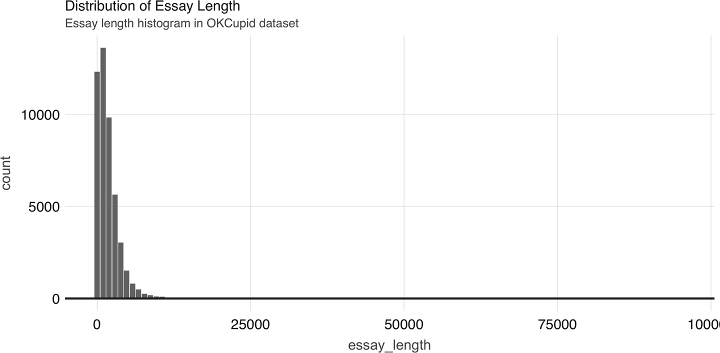
\includegraphics{figures/4_6.png}
\caption{图4-6. 文章长度分布}
\end{figure}

我们会在第5章中使用这个数据集,所以让我们先存成一个Parquet文件,一种数值型数据的高效文件格式:

\begin{Shaded}
\begin{Highlighting}[]
\KeywordTok{spark_write_parquet}\NormalTok{(okc_train, }\StringTok{"data/okc-train.parquet"}\NormalTok{)}
\end{Highlighting}
\end{Shaded}

现在我们有了一些可用的特征,可以进行一些监督式的学习算法。

\hypertarget{ux76d1ux7763ux5f0fux5b66ux4e60}{%
\subsection{监督式学习}\label{ux76d1ux7763ux5f0fux5b66ux4e60}}

一旦我们有了数据集,我们就可以开始构建一些模型。在我们开始之前,需要制定一个计划来调整和验证备选模型。在建模项目中,我们经常尝试不同类型的模型和方法来进行拟合,看看哪一个表现最好。因为我们处理的是一个二分类问题,可用的指标包括准确度,精确度,灵敏度,以及接受者操作特性曲线(ROC
AUC)下的面积,以及其他度量方法。要优化的指标取决于特定业务问题,但是在本次练习中,我们将重点放在ROC
AUC上。

很重要的一点是,我们在最终结束前不要偷看测试集,因为我们获得的任何信息都可能影响我们的建模决策,这会反过来让模型性能估计不够可信。为了调试验证,我们进行10折交叉验证,这是模型的标准调试方法。具体方案如下:首先将数据集划分为10个大致相同的子集。我们把第2到第10组作为训练集,而在第一个集合上验证模型结果。然后,我们把第2组作为验证集,并在第1,第3到第10组上训练算法。最终,我们培训了10个模型,并对性能进行平均。如果时间和资源允许,你还可以使用不同的随机分区多次执行此过程。在我们的例子中,我们进行一次交叉验证。从现在开始,我们把与每个分割相关的训练集称为分析数据,并将验证集作为评估数据。

使用\texttt{sdf\_random\_split()}函数,我们可以构建一系列\texttt{okc\_train}数据表的子集:

\begin{Shaded}
\begin{Highlighting}[]
\NormalTok{vfolds <-}\StringTok{ }\KeywordTok{sdf_random_split}\NormalTok{(okc_train, }\DataTypeTok{weights =}\NormalTok{ purrr}\OperatorTok{::}\KeywordTok{set_names}\NormalTok{(}\KeywordTok{rep}\NormalTok{(}\FloatTok{0.1}\NormalTok{, }\DecValTok{10}\NormalTok{), }\KeywordTok{paste0}\NormalTok{(}\StringTok{"fold"}\NormalTok{, }
    \DecValTok{1}\OperatorTok{:}\DecValTok{10}\NormalTok{)), }\DataTypeTok{seed =} \DecValTok{42}\NormalTok{)}
\end{Highlighting}
\end{Shaded}

然后,我们创建第一次分析/评估数据集分割,代码如下:

\begin{Shaded}
\begin{Highlighting}[]
\NormalTok{analysis_set <-}\StringTok{ }\KeywordTok{do.call}\NormalTok{(rbind, vfolds[}\DecValTok{2}\OperatorTok{:}\DecValTok{10}\NormalTok{])}
\NormalTok{assessment_set <-}\StringTok{ }\NormalTok{vfolds[[}\DecValTok{1}\NormalTok{]]}
\end{Highlighting}
\end{Shaded}

这里我们需要仔细处理的一个问题是变量的缩放。我们需要确保不要把评估集的任何信息泄漏给分析集,所以我们只在分析集上计算平均值和标准差,并对两个集合做相同的转换。以下是我们对\texttt{age}变量所做的操作:

\begin{Shaded}
\begin{Highlighting}[]
\NormalTok{make_scale_age <-}\StringTok{ }\ControlFlowTok{function}\NormalTok{(analysis_data) \{}
\NormalTok{    scale_values <-}\StringTok{ }\NormalTok{analysis_data }\OperatorTok\StringTok{ }\KeywordTok{summarise}\NormalTok{(}\DataTypeTok{mean_age =} \KeywordTok{mean}\NormalTok{(age), }\DataTypeTok{sd_age =} \KeywordTok{sd}\NormalTok{(age)) }\OperatorTok\StringTok{ }
\StringTok{        }\KeywordTok{collect}\NormalTok{()}
    \ControlFlowTok{function}\NormalTok{(data) \{}
\NormalTok{        data }\OperatorTok\StringTok{ }\KeywordTok{mutate}\NormalTok{(}\DataTypeTok{scaled_age =}\NormalTok{ (age }\OperatorTok{-}\StringTok{ }\OperatorTok{!!}\NormalTok{scale_values}\OperatorTok{$}\NormalTok{mean_age)}\OperatorTok{/!!}\NormalTok{scale_values}\OperatorTok{$}\NormalTok{sd_age)}
\NormalTok{    \}}
\NormalTok{\}}
\NormalTok{scale_age <-}\StringTok{ }\KeywordTok{make_scale_age}\NormalTok{(analysis_set)}
\NormalTok{train_set <-}\StringTok{ }\KeywordTok{scale_age}\NormalTok{(analysis_set)}
\NormalTok{validation_set <-}\StringTok{ }\KeywordTok{scale_age}\NormalTok{(assessment_set)}
\end{Highlighting}
\end{Shaded}

为了简洁起见,这里我们只展示如何转换\texttt{age}变量。但是在实践中,你可能希望归一化每一个连续预测变量,例如前一节中导出的\texttt{essay\_length}
变量。

逻辑回归通常是二分类问题的合理起点,所以让我们试试看。假设我们的领域知识给我们提供了一组初始预测变量。然后,我们可以使用\texttt{Formula}接口拟合模型:

\begin{Shaded}
\begin{Highlighting}[]
\NormalTok{lr <-}\StringTok{ }\KeywordTok{ml_logistic_regression}\NormalTok{(}
\NormalTok{analysis_set, not_working }\OperatorTok{~}\StringTok{ }\NormalTok{scaled_age }\OperatorTok{+}\StringTok{ }\NormalTok{sex }\OperatorTok{+}\StringTok{ }\NormalTok{drinks }\OperatorTok{+}\StringTok{ }\NormalTok{drugs }\OperatorTok{+}\StringTok{ }\NormalTok{essay_length}
\NormalTok{)}
\NormalTok{lr}
\NormalTok{Formula}\OperatorTok{:}\StringTok{ }\NormalTok{not_working }\OperatorTok{~}\StringTok{ }\NormalTok{scaled_age }\OperatorTok{+}\StringTok{ }\NormalTok{sex }\OperatorTok{+}\StringTok{ }\NormalTok{drinks }\OperatorTok{+}\StringTok{ }\NormalTok{drugs }\OperatorTok{+}\StringTok{ }\NormalTok{essay_length}
\NormalTok{Coefficients}\OperatorTok{:}
\StringTok{ }\NormalTok{(Intercept) scaled_age sex_m drinks_socially}
 \FloatTok{-2.823517e+00} \FloatTok{-1.309498e+00} \FloatTok{-1.918137e-01} \FloatTok{2.235833e-01}
\NormalTok{ drinks_rarely drinks_often drinks_not at all drinks_missing}
 \FloatTok{6.732361e-01} \FloatTok{7.572970e-02} \FloatTok{8.214072e-01} \FloatTok{-4.456326e-01}
\NormalTok{drinks_very often drugs_never drugs_missing drugs_sometimes}
 \FloatTok{8.032052e-02} \FloatTok{-1.712702e-01} \FloatTok{-3.995422e-01} \FloatTok{-7.483491e-02}
\NormalTok{ essay_length}
 \FloatTok{3.664964e-05}
\end{Highlighting}
\end{Shaded}

要获取评估集的性能度量信息,我们可以使用\texttt{ml\_evaluate()}函数:

\begin{Shaded}
\begin{Highlighting}[]
\NormalTok{validation_summary <-}\StringTok{ }\KeywordTok{ml_evaluate}\NormalTok{(lr, assessment_set)}
\end{Highlighting}
\end{Shaded}

你可以打印\texttt{validation\_summary},查看可用的度量:

\begin{Shaded}
\begin{Highlighting}[]
\NormalTok{validation_summary}
\NormalTok{BinaryLogisticRegressionSummaryImpl}
\NormalTok{ Access the following via }\StringTok{`}\DataTypeTok{$}\StringTok{`}\NormalTok{ or }\StringTok{`}\DataTypeTok{ml_summary()}\StringTok{`}\NormalTok{.}
 \OperatorTok{-}\StringTok{ }\KeywordTok{features_col}\NormalTok{()}
 \OperatorTok{-}\StringTok{ }\KeywordTok{label_col}\NormalTok{()}
 \OperatorTok{-}\StringTok{ }\KeywordTok{predictions}\NormalTok{()}
 \OperatorTok{-}\StringTok{ }\KeywordTok{probability_col}\NormalTok{()}
 \OperatorTok{-}\StringTok{ }\KeywordTok{area_under_roc}\NormalTok{()}
 \OperatorTok{-}\StringTok{ }\KeywordTok{f_measure_by_threshold}\NormalTok{()}
 \OperatorTok{-}\StringTok{ }\KeywordTok{pr}\NormalTok{()}
 \OperatorTok{-}\StringTok{ }\KeywordTok{precision_by_threshold}\NormalTok{()}
 \OperatorTok{-}\StringTok{ }\KeywordTok{recall_by_threshold}\NormalTok{()}
 \OperatorTok{-}\StringTok{ }\KeywordTok{roc}\NormalTok{()}
 \OperatorTok{-}\StringTok{ }\KeywordTok{prediction_col}\NormalTok{()}
 \OperatorTok{-}\StringTok{ }\KeywordTok{accuracy}\NormalTok{()}
 \OperatorTok{-}\StringTok{ }\KeywordTok{f_measure_by_label}\NormalTok{()}
 \OperatorTok{-}\StringTok{ }\KeywordTok{false_positive_rate_by_label}\NormalTok{()}
 \OperatorTok{-}\StringTok{ }\KeywordTok{labels}\NormalTok{()}
 \OperatorTok{-}\StringTok{ }\KeywordTok{precision_by_label}\NormalTok{()}
 \OperatorTok{-}\StringTok{ }\KeywordTok{recall_by_label}\NormalTok{()}
 \OperatorTok{-}\StringTok{ }\KeywordTok{true_positive_rate_by_label}\NormalTok{()}
 \OperatorTok{-}\StringTok{ }\KeywordTok{weighted_f_measure}\NormalTok{()}
 \OperatorTok{-}\StringTok{ }\KeywordTok{weighted_false_positive_rate}\NormalTok{()}
 \OperatorTok{-}\StringTok{ }\KeywordTok{weighted_precision}\NormalTok{()}
 \OperatorTok{-}\StringTok{ }\KeywordTok{weighted_recall}\NormalTok{()}
 \OperatorTok{-}\StringTok{ }\KeywordTok{weighted_true_positive_rate}\NormalTok{()}
\end{Highlighting}
\end{Shaded}

我们可以使用\texttt{validation\_summary\$roc()}的输出和\texttt{ggplot2},绘制ROC曲线:

\begin{Shaded}
\begin{Highlighting}[]
\NormalTok{roc <-}\StringTok{ }\NormalTok{validation_summary}\OperatorTok{$}\KeywordTok{roc}\NormalTok{() }\OperatorTok\StringTok{ }\KeywordTok{collect}\NormalTok{()}
\KeywordTok{ggplot}\NormalTok{(roc, }\KeywordTok{aes}\NormalTok{(}\DataTypeTok{x =}\NormalTok{ FPR, }\DataTypeTok{y =}\NormalTok{ TPR)) }\OperatorTok{+}\StringTok{ }\KeywordTok{geom_line}\NormalTok{() }\OperatorTok{+}\StringTok{ }\KeywordTok{geom_abline}\NormalTok{(}\DataTypeTok{lty =} \StringTok{"dashed"}\NormalTok{)}
\end{Highlighting}
\end{Shaded}

图4-7展示了绘制结果。

ROC曲线绘制了真阳性率(敏感性)与假阳性率(1-特异性)之间的关系,以便反映分类阈值的变化。在实践中,业务问题有助于确定曲线上设置分类阈值的位置。AUC是一种用于确定模型质量的汇总度量,我们可以通过调用\texttt{area\_under\_roc()}函数来计算它。

\begin{figure}
\centering
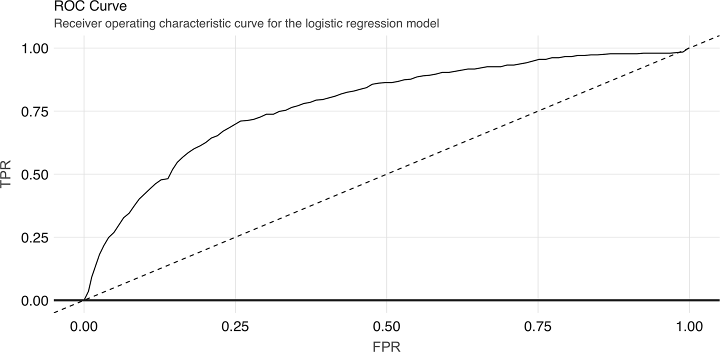
\includegraphics{figures/4_7.png}
\caption{图4-7. 逻辑回归模型的ROC曲线}
\end{figure}

\begin{Shaded}
\begin{Highlighting}[]
\NormalTok{validation_summary}\OperatorTok{$}\KeywordTok{area_under_roc}\NormalTok{()}
\NormalTok{[}\DecValTok{1}\NormalTok{] }\FloatTok{0.7872754}
\end{Highlighting}
\end{Shaded}

\begin{quote}
Spark只为广义线性模型(包括线性模型和逻辑回归)提供了评估方法。对于其他算法,你可以使用评估函数(例如,数据框的\texttt{ml\_binary\_classification\_evaluator()}
,或者是自己的度量算法。
\end{quote}

现在,我们可以轻松的重复这个已经用在分割分析/评估数据集上的逻辑:

\begin{Shaded}
\begin{Highlighting}[]
\NormalTok{cv_results <-}\StringTok{ }\NormalTok{purrr}\OperatorTok{::}\KeywordTok{map_df}\NormalTok{(}\DecValTok{1}\OperatorTok{:}\DecValTok{10}\NormalTok{, }\ControlFlowTok{function}\NormalTok{(v) \{}
\NormalTok{analysis_set <-}\StringTok{ }\KeywordTok{do.call}\NormalTok{(rbind, vfolds[}\KeywordTok{setdiff}\NormalTok{(}\DecValTok{1}\OperatorTok{:}\DecValTok{10}\NormalTok{, v)]) }\OperatorTok\StringTok{ }\KeywordTok{compute}\NormalTok{()}
\NormalTok{assessment_set <-}\StringTok{ }\NormalTok{vfolds[[v]]}
\NormalTok{scale_age <-}\StringTok{ }\KeywordTok{make_scale_age}\NormalTok{(analysis_set)}
\NormalTok{train_set <-}\StringTok{ }\KeywordTok{scale_age}\NormalTok{(analysis_set)}
\NormalTok{validation_set <-}\StringTok{ }\KeywordTok{scale_age}\NormalTok{(assessment_set)}
\NormalTok{model <-}\StringTok{ }\KeywordTok{ml_logistic_regression}\NormalTok{(}
\NormalTok{analysis_set, not_working }\OperatorTok{~}\StringTok{ }\NormalTok{scaled_age }\OperatorTok{+}\StringTok{ }\NormalTok{sex }\OperatorTok{+}\StringTok{ }\NormalTok{drinks }\OperatorTok{+}\StringTok{ }\NormalTok{drugs }\OperatorTok{+}\StringTok{ }\NormalTok{essay_length}
\NormalTok{)s <-}\StringTok{ }\KeywordTok{ml_evaluate}\NormalTok{(model, assessment_set)}
\NormalTok{roc_df <-}\StringTok{ }\NormalTok{s}\OperatorTok{$}\KeywordTok{roc}\NormalTok{() }\OperatorTok
\KeywordTok{collect}\NormalTok{()}
\NormalTok{auc <-}\StringTok{ }\NormalTok{s}\OperatorTok{$}\KeywordTok{area_under_roc}\NormalTok{()}
\KeywordTok{tibble}\NormalTok{(}
\DataTypeTok{Resample =} \KeywordTok{paste0}\NormalTok{(}\StringTok{"Fold"}\NormalTok{, stringr}\OperatorTok{::}\KeywordTok{str_pad}\NormalTok{(v, }\DataTypeTok{width =} \DecValTok{2}\NormalTok{, }\DataTypeTok{pad =} \StringTok{"0"}\NormalTok{)),}
\NormalTok{Supervised Learning }\OperatorTok{|}\StringTok{ }\DecValTok{69}
\DataTypeTok{roc_df =} \KeywordTok{list}\NormalTok{(roc_df),}
\DataTypeTok{auc =}\NormalTok{ auc}
\NormalTok{)}
\NormalTok{\})}
\end{Highlighting}
\end{Shaded}

这会返回10条ROC曲线:

\begin{Shaded}
\begin{Highlighting}[]
\KeywordTok{unnest}\NormalTok{(cv_results, roc_df) }\OperatorTok\StringTok{ }\KeywordTok{ggplot}\NormalTok{(}\KeywordTok{aes}\NormalTok{(}\DataTypeTok{x =}\NormalTok{ FPR, }\DataTypeTok{y =}\NormalTok{ TPR, }\DataTypeTok{color =}\NormalTok{ Resample)) }\OperatorTok{+}\StringTok{ }
\StringTok{    }\KeywordTok{geom_line}\NormalTok{() }\OperatorTok{+}\StringTok{ }\KeywordTok{geom_abline}\NormalTok{(}\DataTypeTok{lty =} \StringTok{"dashed"}\NormalTok{)}
\end{Highlighting}
\end{Shaded}

图4-8展示了绘图结果:

\begin{figure}
\centering
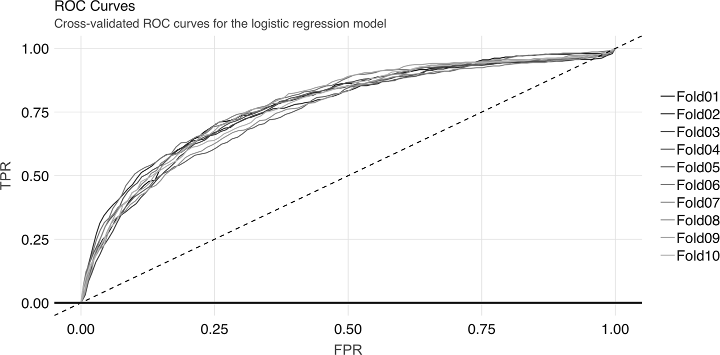
\includegraphics{figures/4_8.png}
\caption{图4-8. 逻辑回归模型的交叉验证ROC曲线}
\end{figure}

我们可以获取AUC度量的平均值:

\begin{Shaded}
\begin{Highlighting}[]
\KeywordTok{mean}\NormalTok{(cv_results}\OperatorTok{$}\NormalTok{auc)}
\NormalTok{[}\DecValTok{1}\NormalTok{] }\FloatTok{0.7715102}
\end{Highlighting}
\end{Shaded}

\hypertarget{ux5e7fux4e49ux7ebfux6027ux56deux5f52}{%
\subsubsection{广义线性回归}\label{ux5e7fux4e49ux7ebfux6027ux56deux5f52}}

如果你对广义线性模型(generalized linear
model,GLM)诊断感兴趣,你也可以通过广义线性回归接口,给定\texttt{family=\ "binomial"},拟合一个逻辑回归模型。因为结果是一个回归模型,\texttt{ml\_predict()}方法不会给出类别概率。但是它包含了置信区间,可以进行系数估计:

\begin{Shaded}
\begin{Highlighting}[]
\NormalTok{glr <-}\StringTok{ }\KeywordTok{ml_generalized_linear_regression}\NormalTok{(analysis_set, not_working }\OperatorTok{~}\StringTok{ }\NormalTok{scaled_age }\OperatorTok{+}\StringTok{ }
\StringTok{    }\NormalTok{sex }\OperatorTok{+}\StringTok{ }\NormalTok{drinks }\OperatorTok{+}\StringTok{ }\NormalTok{drugs, }\DataTypeTok{family =} \StringTok{"binomial"}\NormalTok{)}
\NormalTok{tidy_glr <-}\StringTok{ }\KeywordTok{tidy}\NormalTok{(glr)}
\end{Highlighting}
\end{Shaded}

我们可以把置信估计存到一个整齐的数据框中,以便进一步处理。例如,创建一个系数绘图,如图4-9所示:

\begin{Shaded}
\begin{Highlighting}[]
\NormalTok{tidy_glr }\OperatorTok\StringTok{ }\KeywordTok{ggplot}\NormalTok{(}\KeywordTok{aes}\NormalTok{(}\DataTypeTok{x =}\NormalTok{ term, }\DataTypeTok{y =}\NormalTok{ estimate)) }\OperatorTok{+}\StringTok{ }\KeywordTok{geom_point}\NormalTok{() }\OperatorTok{+}\StringTok{ }\KeywordTok{geom_errorbar}\NormalTok{(}\KeywordTok{aes}\NormalTok{(}\DataTypeTok{ymin =}\NormalTok{ estimate }\OperatorTok{-}\StringTok{ }
\StringTok{    }\FloatTok{1.96} \OperatorTok{*}\StringTok{ }\NormalTok{std.error, }\DataTypeTok{ymax =}\NormalTok{ estimate }\OperatorTok{+}\StringTok{ }\FloatTok{1.96} \OperatorTok{*}\StringTok{ }\NormalTok{std.error, }\DataTypeTok{width =} \FloatTok{0.1}\NormalTok{)) }\OperatorTok{+}\StringTok{ }\KeywordTok{coord_flip}\NormalTok{() }\OperatorTok{+}\StringTok{ }
\StringTok{    }\KeywordTok{geom_hline}\NormalTok{(}\DataTypeTok{yintercept =} \DecValTok{0}\NormalTok{, }\DataTypeTok{linetype =} \StringTok{"dashed"}\NormalTok{)}
\end{Highlighting}
\end{Shaded}

\begin{figure}
\centering
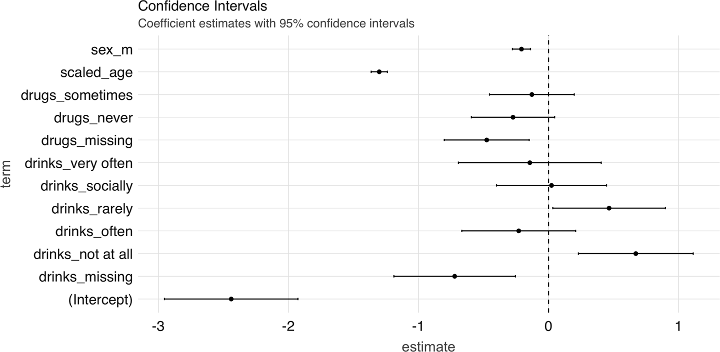
\includegraphics{figures/4_9.png}
\caption{图4-9. 95\%置信区间的系数估计}
\end{figure}

\begin{quote}
\texttt{ml\_logistic\_regression()}和\texttt{ml\_linear\_regression()}都支持通过\texttt{reg\_param}和\texttt{elastic\_net\_param}参数,实现弹性网正则化\footnote{Zou
  H, Hastie T (2005). ``Regularization and variable selection via the
  elastic net.'' Journal of the royal statistical society: series B
  (statistical methodology), 67(2), 301--320.}。\texttt{reg\_param}对应\(\lambda\),而\texttt{elastic\_net\_param}对应\(\alpha\)。\texttt{ml\_generalized\_linear\_regression()}只支持\texttt{reg\_param}。
\end{quote}

\hypertarget{ux5176ux5b83ux6a21ux578b}{%
\subsubsection{其它模型}\label{ux5176ux5b83ux6a21ux578b}}

Spark支持许多标准的建模算法,很容易为特定问题应用这些模型和超参数(控制模型拟合过程的值)。你可以在附录中找到支持ML相关函数的列表。访问这些功能的接口大部分是相同的,因此很容易进行实验。例如,为了拟合神经网络模型,我们可以运行以下命令:

\begin{Shaded}
\begin{Highlighting}[]
\NormalTok{nn <-}\StringTok{ }\KeywordTok{ml_multilayer_perceptron_classifier}\NormalTok{(analysis_set, not_working }\OperatorTok{~}\StringTok{ }\NormalTok{scaled_age }\OperatorTok{+}\StringTok{ }
\StringTok{    }\NormalTok{sex }\OperatorTok{+}\StringTok{ }\NormalTok{drinks }\OperatorTok{+}\StringTok{ }\NormalTok{drugs }\OperatorTok{+}\StringTok{ }\NormalTok{essay_length, }\DataTypeTok{layers =} \KeywordTok{c}\NormalTok{(}\DecValTok{12}\NormalTok{, }\DecValTok{64}\NormalTok{, }\DecValTok{64}\NormalTok{, }\DecValTok{2}\NormalTok{))}
\end{Highlighting}
\end{Shaded}

这返回一个前馈神经网络模型,它有两个隐藏层,每层64个节点。注意,必须在\texttt{layers}参数中为输入和输出层指定正确的值。我们可以使用\texttt{ml\_predict()}在验证集上获取预测值:

\begin{Shaded}
\begin{Highlighting}[]
\NormalTok{predictions <-}\StringTok{ }\KeywordTok{ml_predict}\NormalTok{(nn, assessment_set)}
\end{Highlighting}
\end{Shaded}

然后,我们可以通过\texttt{ml\_binary\_classification\_evaluator()}计算AUC:

\begin{Shaded}
\begin{Highlighting}[]
\KeywordTok{ml_binary_classification_evaluator}\NormalTok{(predictions)}
\NormalTok{[}\DecValTok{1}\NormalTok{] }\FloatTok{0.7812709}
\end{Highlighting}
\end{Shaded}

到目前为止,我们还没有查看文章字段中的非结构化文本,只是做了一些简单的字符计数。在下一节中,我们会具体探索文本数据。

\hypertarget{ux975eux76d1ux7763ux5f0fux5b66ux4e60}{%
\subsection{非监督式学习}\label{ux975eux76d1ux7763ux5f0fux5b66ux4e60}}

除了语音、图像和视频之外,文本数据也是大数据爆炸的表现之一。在现代文本挖掘技术和计算资源之前,公司很少使用自由格式的文本字段。今天,文本被认为是一个丰富的无处不在的信息来源,从医生的笔记到客户的投诉。在本节中,我们将展示一些\texttt{sparklyr}基本的文本分析能力。如果想了解文本挖掘技术的更多背景知识,我们建议阅读David
Robinson和Julie Silge的《R文本挖掘》(O'Reilly)。

在本节中,我们将展示如何对OKCupid数据集中的文章数据进行基本的主题建模任务。我们的计划是连接每个用户的文章字段(其中有10个),并将每个用户看成为一个文档,然后尝试使用隐狄利克雷分布(Latent
Dirichlet Allocation ,LDA)来发现主题(我们很快会定义这些主题)。

\hypertarget{ux6570ux636eux51c6ux5907}{%
\subsubsection{数据准备}\label{ux6570ux636eux51c6ux5907}}

和往常一样,在分析一个数据集(或其中的一个子集)之前,我们希望快速地查看它以便确定自己的方向。在这种情况下,我们关注用户在约会档案中输入的自由格式文本。

\begin{Shaded}
\begin{Highlighting}[]
\NormalTok{essay_cols <-}\StringTok{ }\KeywordTok{paste0}\NormalTok{(}\StringTok{"essay"}\NormalTok{, }\DecValTok{0}\OperatorTok{:}\DecValTok{9}\NormalTok{)}
\NormalTok{essays <-}\StringTok{ }\NormalTok{okc }\OperatorTok
\KeywordTok{select}\NormalTok{(}\OperatorTok{!!}\NormalTok{essay_cols)}
\NormalTok{essays }\OperatorTok
\KeywordTok{glimpse}\NormalTok{()}
\NormalTok{Observations}\OperatorTok{:}\StringTok{ }\NormalTok{??}
\NormalTok{Variables}\OperatorTok{:}\StringTok{ }\DecValTok{10}
\NormalTok{Database}\OperatorTok{:}\StringTok{ }\NormalTok{spark_connection}
\OperatorTok{$}\StringTok{ }\NormalTok{essay0 }\OperatorTok{<}\NormalTok{chr}\OperatorTok{>}\StringTok{ "about me:<br />}\CharTok{\textbackslash{}n}\StringTok{<br />}\CharTok{\textbackslash{}n}\StringTok{i would love to think that…}
\StringTok{$ essay1 <chr> "}\NormalTok{currently working as an international agent }\ControlFlowTok{for}\NormalTok{ a f…}
\OperatorTok{$}\StringTok{ }\NormalTok{essay2 }\OperatorTok{<}\NormalTok{chr}\OperatorTok{>}\StringTok{ "making people laugh.<br />}\CharTok{\textbackslash{}n}\StringTok{ranting about a good sa…}
\StringTok{$ essay3 <chr> "}\NormalTok{the way i look. i am a six foot half asian, half ca…}
\OperatorTok{$}\StringTok{ }\NormalTok{essay4 }\OperatorTok{<}\NormalTok{chr}\OperatorTok{>}\StringTok{ "books:<br />}\CharTok{\textbackslash{}n}\StringTok{absurdistan, the republic, of mice an…}
\StringTok{$ essay5 <chr> "}\NormalTok{food.}\OperatorTok{<}\NormalTok{br }\OperatorTok{/}\ErrorTok{>}\NormalTok{\textbackslash{}nwater.}\OperatorTok{<}\NormalTok{br }\OperatorTok{/}\ErrorTok{>}\NormalTok{\textbackslash{}ncell phone.}\OperatorTok{<}\NormalTok{br }\OperatorTok{/}\ErrorTok{>}\NormalTok{\textbackslash{}nshelt…}
\OperatorTok{$}\StringTok{ }\NormalTok{essay6 }\OperatorTok{<}\NormalTok{chr}\OperatorTok{>}\StringTok{ "duality and humorous things"}\NormalTok{, }\StringTok{"missing"}\NormalTok{, }\StringTok{"missing"}\NormalTok{,…}
\OperatorTok{$}\StringTok{ }\NormalTok{essay7 }\OperatorTok{<}\NormalTok{chr}\OperatorTok{>}\StringTok{ "trying to find someone to hang out with. i am down …}
\StringTok{$ essay8 <chr> "}\NormalTok{i am new to california and looking }\ControlFlowTok{for}\NormalTok{ someone to w…}
\OperatorTok{$}\StringTok{ }\NormalTok{essay9 }\OperatorTok{<}\NormalTok{chr}\OperatorTok{>}\StringTok{ "you want to be swept off your feet!<br />}\CharTok{\textbackslash{}n}\StringTok{you are …}
\end{Highlighting}
\end{Shaded}

从这些输出,我们看到:

\begin{itemize}
\tightlist
\item
  文本包含HTML标签。
\item
  文本包含换行符(\textbackslash n)。
\item
  数据中有缺失值。
\end{itemize}

HTML标记和特殊字符会污染数据,因为它们不是用户直接输入的,也不提供有意义的信息。类似地,由于我们已经用\emph{missing}字符串对丢失的字符字段进行了编码,所以需要删除它。(注意,这样还将删除用户编写的单词``missing''的实例,但删除过程中丢失的信息可能很小。)

当你分析自己的文本数据时,你会很快发现并熟悉特定数据集的独有性质。与表格数值数据一样,预处理文本数据是一个迭代的过程。经过几次尝试之后,我们得到以下转换结果:

\begin{Shaded}
\begin{Highlighting}[]
\NormalTok{essays <-}\StringTok{ }\NormalTok{essays }\OperatorTok\StringTok{ }\CommentTok{# Replace `missing` with empty string.}
\KeywordTok{mutate_all}\NormalTok{(}\KeywordTok{list}\NormalTok{(}\OperatorTok{~}\KeywordTok{ifelse}\NormalTok{(. }\OperatorTok{==}\StringTok{ "missing"}\NormalTok{, }\StringTok{""}\NormalTok{, .))) }\OperatorTok\StringTok{ }\CommentTok{# Concatenate the columns.}
\KeywordTok{mutate}\NormalTok{(}\DataTypeTok{essay =} \KeywordTok{paste}\NormalTok{(}\OperatorTok{!!!}\KeywordTok{syms}\NormalTok{(essay_cols))) }\OperatorTok\StringTok{ }\CommentTok{# Remove miscellaneous characters and HTML tags}
\KeywordTok{mutate}\NormalTok{(}\DataTypeTok{words =} \KeywordTok{regexp_replace}\NormalTok{(essay, }\StringTok{"}\CharTok{\textbackslash{}\textbackslash{}}\StringTok{n|&nbsp;|<[^>]*>|[^A-Za-z|']"}\NormalTok{, }\StringTok{" "}\NormalTok{))}
\end{Highlighting}
\end{Shaded}

这里注意我们使用\texttt{regex\_replace()},它是一个Spark的SQL函数。下面,我们讨论LDA以及如何应用到干净的数据集上。

\hypertarget{ux4e3bux9898ux5efaux6a21}{%
\subsubsection{主题建模}\label{ux4e3bux9898ux5efaux6a21}}

LDA是一种主题模型,用于识别一组文档中的抽象``主题''。它是一种无监督的算法,因为我们不给输入文档提供任何标签或主题。LDA假设每个文档都是主题的混合体,并且主题是词的混合体。在训练阶段,它试图同时估计这两个变量。主题模型的典型用例包括对许多文档进行分类,这些文档由于量大使得手动方法不可行。应用领域从GitHub问题到法律文档。

在我们遵循上一节的工作流,得到一个非常干净的数据集之后,可以用\texttt{ml\_lda()}来拟合LDA模型:

\begin{Shaded}
\begin{Highlighting}[]
\NormalTok{stop_words <-}\StringTok{ }\KeywordTok{ml_default_stop_words}\NormalTok{(sc) }\OperatorTok\StringTok{ }\KeywordTok{c}\NormalTok{(}\StringTok{"like"}\NormalTok{, }\StringTok{"love"}\NormalTok{, }\StringTok{"good"}\NormalTok{, }\StringTok{"music"}\NormalTok{, }\StringTok{"friends"}\NormalTok{, }
    \StringTok{"people"}\NormalTok{, }\StringTok{"life"}\NormalTok{, }\StringTok{"time"}\NormalTok{, }\StringTok{"things"}\NormalTok{, }\StringTok{"food"}\NormalTok{, }\StringTok{"really"}\NormalTok{, }\StringTok{"also"}\NormalTok{, }\StringTok{"movies"}\NormalTok{)}
\NormalTok{lda_model <-}\StringTok{ }\KeywordTok{ml_lda}\NormalTok{(essays, }\OperatorTok{~}\NormalTok{words, }\DataTypeTok{k =} \DecValTok{6}\NormalTok{, }\DataTypeTok{max_iter =} \DecValTok{1}\NormalTok{, }\DataTypeTok{min_token_length =} \DecValTok{4}\NormalTok{, }\DataTypeTok{stop_words =}\NormalTok{ stop_words, }
    \DataTypeTok{min_df =} \DecValTok{5}\NormalTok{)}
\end{Highlighting}
\end{Shaded}

我们还需要一个\texttt{stop\_words}向量,由常用的英语单词和我们数据集中常见的单词组成,它会告诉算法忽略它们。在模型拟合之后,我们可以使用\texttt{tidy()}函数从模型中提取相关的\texttt{beta},即每个主题中每个单词的概率。

\begin{Shaded}
\begin{Highlighting}[]
\NormalTok{betas <-}\StringTok{ }\KeywordTok{tidy}\NormalTok{(lda_model)}
\NormalTok{betas}
\CommentTok{# A tibble: 256,992 x 3}
\NormalTok{ topic term beta}
 \OperatorTok{<}\NormalTok{int}\OperatorTok{>}\StringTok{ }\ErrorTok{<}\NormalTok{chr}\OperatorTok{>}\StringTok{ }\ErrorTok{<}\NormalTok{dbl}\OperatorTok{>}
\StringTok{ }\DecValTok{1} \DecValTok{0}\NormalTok{ know }\FloatTok{303.}
 \DecValTok{2} \DecValTok{0}\NormalTok{ work }\FloatTok{250.}
 \DecValTok{3} \DecValTok{0}\NormalTok{ want }\FloatTok{367.}
 \DecValTok{4} \DecValTok{0}\NormalTok{ books }\FloatTok{211.}
 \DecValTok{5} \DecValTok{0}\NormalTok{ family }\FloatTok{213.}
 \DecValTok{6} \DecValTok{0}\NormalTok{ think }\FloatTok{291.}
 \DecValTok{7} \DecValTok{0}\NormalTok{ going }\FloatTok{160.}
 \DecValTok{8} \DecValTok{0}\NormalTok{ anything }\FloatTok{292.}
 \DecValTok{9} \DecValTok{0}\NormalTok{ enjoy }\FloatTok{145.}
\DecValTok{10} \DecValTok{0}\NormalTok{ much }\FloatTok{272.}
\CommentTok{# … with 256,982 more rows}
\end{Highlighting}
\end{Shaded}

然后,我们可以按主题查看单词概率来可视化输出。在图4-10和图4-11中,我们显示了1次迭代和100次迭代的结果。下面是生成图4-10的代码;要生成图4-11,您需要在运行\texttt{ml\_lda()}时设置\texttt{max\_iter\ =\ 100},但要注意在单机上这可能需要长时间------这是一个大计算问题,而一个合适Spark集群可以很容易地解决。

\begin{Shaded}
\begin{Highlighting}[]
\NormalTok{betas }\OperatorTok\StringTok{ }\KeywordTok{group_by}\NormalTok{(topic) }\OperatorTok\StringTok{ }\KeywordTok{top_n}\NormalTok{(}\DecValTok{10}\NormalTok{, beta) }\OperatorTok\StringTok{ }\KeywordTok{ungroup}\NormalTok{() }\OperatorTok\StringTok{ }\KeywordTok{arrange}\NormalTok{(topic, }\OperatorTok{-}\NormalTok{beta) }\OperatorTok\StringTok{ }
\StringTok{    }\KeywordTok{mutate}\NormalTok{(}\DataTypeTok{term =} \KeywordTok{reorder}\NormalTok{(term, beta)) }\OperatorTok\StringTok{ }\KeywordTok{ggplot}\NormalTok{(}\KeywordTok{aes}\NormalTok{(term, beta, }\DataTypeTok{fill =} \KeywordTok{factor}\NormalTok{(topic))) }\OperatorTok{+}\StringTok{ }
\StringTok{    }\KeywordTok{geom_col}\NormalTok{(}\DataTypeTok{show.legend =} \OtherTok{FALSE}\NormalTok{) }\OperatorTok{+}\StringTok{ }\KeywordTok{facet_wrap}\NormalTok{(}\OperatorTok{~}\NormalTok{topic, }\DataTypeTok{scales =} \StringTok{"free"}\NormalTok{) }\OperatorTok{+}\StringTok{ }\KeywordTok{coord_flip}\NormalTok{()}
\end{Highlighting}
\end{Shaded}

\begin{figure}
\centering
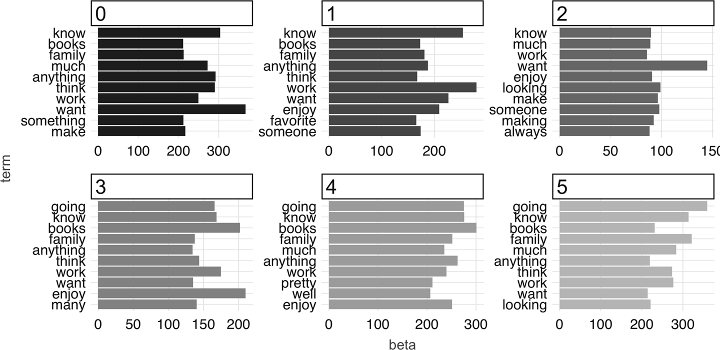
\includegraphics{figures/4_10.png}
\caption{图4-10. 第1次迭代后,每个主题最常用的词语}
\end{figure}

在100次迭代中,我们可以看到``主题''开始出现。如果你正在挖掘大量不熟悉的文档,这本身就是一个有趣的信息。学到的主题也可以作为下游监督学习任务的特征;例如,我们可以考虑在模型中使用主题编号作为预测变量,在我们的预测建模例子

\begin{figure}
\centering
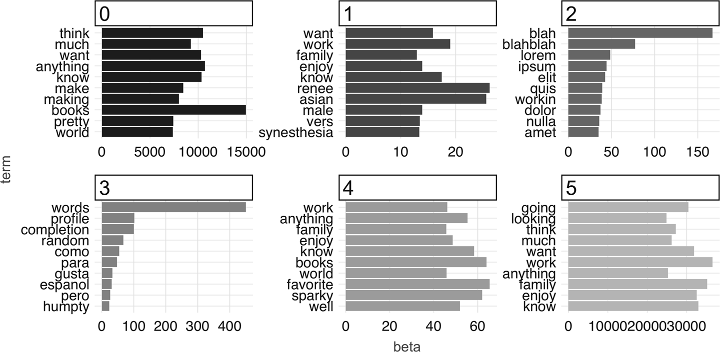
\includegraphics{figures/4_11.png}
\caption{图4-11. 第100次迭代后,每个主题最常用的词语}
\end{figure}

最后,要结束本章,你应该断开Spark连接。第5章也会使用\texttt{OKCupid}数据集,但是我们会从零开始,介绍如何重新加载它:

\begin{Shaded}
\begin{Highlighting}[]
\KeywordTok{spark_disconnect}\NormalTok{(sc)}
\end{Highlighting}
\end{Shaded}

\hypertarget{ux5c0fux7ed3-3}{%
\subsection{小结}\label{ux5c0fux7ed3-3}}

在本章中,我们介绍了用R在Spark中构建预测模型的基础知识,包括EDA、特征工程和构建监督式模型,我们探索了逻辑回归和神经网络,模型。这只是Spark中通过\texttt{MLlib}提供的几十种模型中的一小部分。

然后我们探索了如何使用无监督式学习来处理原始文本。我们创建了一个主题模型,该模型自动将文档分为六个类别。我们介绍了使用一台机器构建主题模型会需要花费大量的时间。这几乎是引入全功能计算集群的完美理由。但要注意:我们首先需要考虑如何自动化数据科学工作流程。

正如我们在介绍本章时提到的,本章重点是预测建模。Spark可以助力大规模数据科学项目,也可以产品化数据科学工作流程,使之可以自动化,也就是我们熟知的机器学习。第5章介绍工具,让预测模型,以及整个训练流程,融合到自动化环境中,可以持续的运行,或者导出到web应用程序、移动应用程序和其他环境中。

\begin{center}\rule{0.5\linewidth}{\linethickness}\end{center}

\hypertarget{ux7b2c5ux7ae0-ux7ba1ux9053ux64cdux4f5c}{%
\section{第5章 管道操作}\label{ux7b2c5ux7ae0-ux7ba1ux9053ux64cdux4f5c}}

\begin{quote}
You will never walk again, but you will fly! ---Three-Eyed Raven
\end{quote}

在第4章中,你学习了如何使用Spark提供的高级函数以及与Spark协同工作的著名R程序包,来构建预测模型。你首先学习了监督式算法,最后学习了原始文本上的非监督式算法。

在本章中,我们将深入学习Spark管道操作,这是第四章中介绍的特征工程的动力。例如,当通过R中的公式接口调用\texttt{MLlib}函数时,例如\texttt{ml\_logistic\_regression(cars,\ am\ \textasciitilde{}\ .)},一个\emph{管道}就在背后构建完成了。因此,管道允许使用高级数据处理和建模流程。此外,管道还允许将其\emph{部署}到生产系统,web应用程序、移动应用程序等,促进了跨数据科学和工程团队的协作。

本章也是鼓励使用本地计算机作为Spark集群的最后一章。你离真正的集群计算,以及数据科学或机器学习只有一章之遥,它们可以扩展到最苛刻的计算问题上。

\hypertarget{ux6982ux8ff0-4}{%
\subsection{概述}\label{ux6982ux8ff0-4}}

管道的构件是称为\emph{转换器}和\emph{评估器}的对象,它们统称为\emph{管道阶段}。转换器可将转换操作应用于数据框并返回另一个数据框;生成的数据框通常包含原始数据框及其追加的新列。另一方面,估计器可以用来创建一个提供训练数据的转换器。考虑下面的例子来说明这种关系:一个``中心和扩展``估计器可以学习一些数据的平均值和标准差,并将统计信息存储在最后的转换器对象中;然后,可以使用这个转换器来归一化它所训练的数据以及任何新的、但看不见的数据。

这里是定义一个评估器的过程:

\begin{Shaded}
\begin{Highlighting}[]
\KeywordTok{library}\NormalTok{(sparklyr)}
\KeywordTok{library}\NormalTok{(dplyr)}
\NormalTok{sc <-}\StringTok{ }\KeywordTok{spark_connect}\NormalTok{(}\DataTypeTok{master =} \StringTok{"local"}\NormalTok{, }\DataTypeTok{version =} \StringTok{"2.3"}\NormalTok{)}
\NormalTok{scaler <-}\StringTok{ }\KeywordTok{ft_standard_scaler}\NormalTok{(}
\NormalTok{sc,}
\DataTypeTok{input_col =} \StringTok{"features"}\NormalTok{,}
\DataTypeTok{output_col =} \StringTok{"features_scaled"}\NormalTok{,}
\DataTypeTok{with_mean =} \OtherTok{TRUE}\NormalTok{)}
\NormalTok{scaler}
\KeywordTok{StandardScaler}\NormalTok{ (Estimator)}
\OperatorTok{<}\NormalTok{standard_scaler_7f6d46f452a1}\OperatorTok{>}
\StringTok{ }\NormalTok{(Parameters }\OperatorTok{--}\StringTok{ }\NormalTok{Column Names)}
\NormalTok{ input_col}\OperatorTok{:}\StringTok{ }\NormalTok{features}
\NormalTok{ output_col}\OperatorTok{:}\StringTok{ }\NormalTok{features_scaled}
\NormalTok{ (Parameters)}
\NormalTok{ with_mean}\OperatorTok{:}\StringTok{ }\OtherTok{TRUE}
\NormalTok{ with_std}\OperatorTok{:}\StringTok{ }\OtherTok{TRUE}
\end{Highlighting}
\end{Shaded}

现在我们可以创建一些数据(我们已经知道平均值和标准差),然后使用\texttt{ml\_fit()}函数拟合扩展模型:

\begin{Shaded}
\begin{Highlighting}[]
\NormalTok{df <-}\StringTok{ }\KeywordTok{copy_to}\NormalTok{(sc, }\KeywordTok{data.frame}\NormalTok{(}\DataTypeTok{value =} \KeywordTok{rnorm}\NormalTok{(}\DecValTok{100000}\NormalTok{))) }\OperatorTok
\KeywordTok{ft_vector_assembler}\NormalTok{(}\DataTypeTok{input_cols =} \StringTok{"value"}\NormalTok{, }\DataTypeTok{output_col =} \StringTok{"features"}\NormalTok{)}
\NormalTok{scaler_model <-}\StringTok{ }\KeywordTok{ml_fit}\NormalTok{(scaler, df)}
\NormalTok{scaler_model}
\KeywordTok{StandardScalerModel}\NormalTok{ (Transformer)}
\OperatorTok{<}\NormalTok{standard_scaler_7f6d46f452a1}\OperatorTok{>}
\StringTok{ }\NormalTok{(Parameters }\OperatorTok{--}\StringTok{ }\NormalTok{Column Names)}
\NormalTok{ input_col}\OperatorTok{:}\StringTok{ }\NormalTok{features}
\NormalTok{ output_col}\OperatorTok{:}\StringTok{ }\NormalTok{features_scaled}
\NormalTok{ (Transformer Info)}
\NormalTok{ mean}\OperatorTok{:}\StringTok{ }\NormalTok{num }\FloatTok{0.00421}
\NormalTok{ std}\OperatorTok{:}\StringTok{ }\NormalTok{num }\FloatTok{0.999}
\end{Highlighting}
\end{Shaded}

\begin{quote}
在Spark
ML中,许多算法和特征变换都要求输入为矢量列。函数\texttt{ft\_vector\_assembler()}执行此任务。你还可以使用该函数初始化要在管道中使用的转换器。
\end{quote}

我们看到,平均值和标准差分别非常接近0和1,这正是我们期望的。借助\texttt{ml\_transform()}函数,我们可以使用转换器来转换数据框:

\begin{Shaded}
\begin{Highlighting}[]
\NormalTok{scaler_model }\OperatorTok
\KeywordTok{ml_transform}\NormalTok{(df) }\OperatorTok
\KeywordTok{glimpse}\NormalTok{()}
\NormalTok{Observations}\OperatorTok{:}\StringTok{ }\NormalTok{??}
\NormalTok{Variables}\OperatorTok{:}\StringTok{ }\DecValTok{3}
\NormalTok{Database}\OperatorTok{:}\StringTok{ }\NormalTok{spark_connection}
\OperatorTok{$}\StringTok{ }\NormalTok{value }\OperatorTok{<}\NormalTok{dbl}\OperatorTok{>}\StringTok{ }\FloatTok{0.75373300}\NormalTok{, }\FloatTok{-0.84207731}\NormalTok{, }\FloatTok{0.59365113}\NormalTok{, }\OperatorTok{-}\NormalTok{…}
\OperatorTok{$}\StringTok{ }\NormalTok{features }\OperatorTok{<}\NormalTok{list}\OperatorTok{>}\StringTok{ }\NormalTok{[}\FloatTok{0.753733}\NormalTok{, }\FloatTok{-0.8420773}\NormalTok{, }\FloatTok{0.5936511}\NormalTok{, }\FloatTok{-0.}\NormalTok{…}
\OperatorTok{$}\StringTok{ }\NormalTok{features_scaled }\OperatorTok{<}\NormalTok{list}\OperatorTok{>}\StringTok{ }\NormalTok{[}\FloatTok{0.7502211}\NormalTok{, }\FloatTok{-0.8470762}\NormalTok{, }\FloatTok{0.58999}\NormalTok{, }\FloatTok{-0.4}\NormalTok{…}
\end{Highlighting}
\end{Shaded}

既然你已经有了基本的评估器和转换器例子。我们继续介绍管道。

\hypertarget{ux521bux5efaux5de5ux4f5c}{%
\subsection{创建工作}\label{ux521bux5efaux5de5ux4f5c}}

一个\emph{管道}是一系列转换器和评估器,一个\emph{管道模型}是在数据上完成训练的一个管道。因此,所有部件都变成了转换器。

在\texttt{sparklyr}中,有两种方法构建管道,二者都使用\texttt{ml\_pipeline()}函数。

我们可以使用\texttt{ml\_pipeline(sc)}初始化空管道,并追加一些阶段:

\begin{Shaded}
\begin{Highlighting}[]
\KeywordTok{ml_pipeline}\NormalTok{(sc) }\OperatorTok
\KeywordTok{ft_standard_scaler}\NormalTok{(}
\DataTypeTok{input_col =} \StringTok{"features"}\NormalTok{,}
\DataTypeTok{output_col =} \StringTok{"features_scaled"}\NormalTok{,}
\DataTypeTok{with_mean =} \OtherTok{TRUE}\NormalTok{)}
\KeywordTok{Pipeline}\NormalTok{ (Estimator) with }\DecValTok{1}\NormalTok{ stage}
\OperatorTok{<}\NormalTok{pipeline_7f6d6a6a38ee}\OperatorTok{>}
\StringTok{ }\NormalTok{Stages}
 \OperatorTok{|--}\DecValTok{1} \KeywordTok{StandardScaler}\NormalTok{ (Estimator)}
 \OperatorTok{|}\StringTok{ }\ErrorTok{<}\NormalTok{standard_scaler_7f6d63bfc7d6}\OperatorTok{>}
\StringTok{ }\ErrorTok{|}\StringTok{ }\NormalTok{(Parameters }\OperatorTok{--}\StringTok{ }\NormalTok{Column Names)}
 \OperatorTok{|}\StringTok{ }\NormalTok{input_col}\OperatorTok{:}\StringTok{ }\NormalTok{features}
 \OperatorTok{|}\StringTok{ }\NormalTok{output_col}\OperatorTok{:}\StringTok{ }\NormalTok{features_scaled}
 \OperatorTok{|}\StringTok{ }\NormalTok{(Parameters)}
 \OperatorTok{|}\StringTok{ }\NormalTok{with_mean}\OperatorTok{:}\StringTok{ }\OtherTok{TRUE}
 \OperatorTok{|}\StringTok{ }\NormalTok{with_std}\OperatorTok{:}\StringTok{ }\OtherTok{TRUE}
\end{Highlighting}
\end{Shaded}

或者,我们也可以直接把阶段传给\texttt{ml\_pipeline()}:

\begin{Shaded}
\begin{Highlighting}[]
\NormalTok{pipeline <-}\StringTok{ }\KeywordTok{ml_pipeline}\NormalTok{(scaler)}
\end{Highlighting}
\end{Shaded}

我们按照拟合评估器的方式,拟合一个管道:

\begin{Shaded}
\begin{Highlighting}[]
\NormalTok{pipeline_model <-}\StringTok{ }\KeywordTok{ml_fit}\NormalTok{(pipeline, df)}
\NormalTok{pipeline_model}
\KeywordTok{PipelineModel}\NormalTok{ (Transformer) with }\DecValTok{1}\NormalTok{ stage}
\OperatorTok{<}\NormalTok{pipeline_7f6d64df6e45}\OperatorTok{>}
\StringTok{ }\NormalTok{Stages}
 \OperatorTok{|--}\DecValTok{1} \KeywordTok{StandardScalerModel}\NormalTok{ (Transformer)}
 \OperatorTok{|}\StringTok{ }\ErrorTok{<}\NormalTok{standard_scaler_7f6d46f452a1}\OperatorTok{>}
\StringTok{ }\ErrorTok{|}\StringTok{ }\NormalTok{(Parameters }\OperatorTok{--}\StringTok{ }\NormalTok{Column Names)}
 \OperatorTok{|}\StringTok{ }\NormalTok{input_col}\OperatorTok{:}\StringTok{ }\NormalTok{features}
 \OperatorTok{|}\StringTok{ }\NormalTok{output_col}\OperatorTok{:}\StringTok{ }\NormalTok{features_scaled}
 \OperatorTok{|}\StringTok{ }\NormalTok{(Transformer Info)}
 \OperatorTok{|}\StringTok{ }\NormalTok{mean}\OperatorTok{:}\StringTok{ }\NormalTok{num }\FloatTok{0.00421}
 \OperatorTok{|}\StringTok{ }\NormalTok{std}\OperatorTok{:}\StringTok{ }\NormalTok{num }\FloatTok{0.999}
\NormalTok{pipeline}
\end{Highlighting}
\end{Shaded}

\begin{quote}
由于Spark
ML的设计,即使管道只包含转换器,它也始终看成是评估器对象。这意味着,如果有一个只有转换器的管道,你仍然需要对其调用\texttt{ml\_fit()},以获得一个转换器。本例中的``拟合''过程实际上不会修改任何转换器。
\end{quote}

\hypertarget{ux7528ux4f8b}{%
\subsection{用例}\label{ux7528ux4f8b}}

既然你已经了解了ML管道的基本概念,那么让我们把它们用到上一章中的预测建模问题。在上一章中,我们试图通过查看人们的画像来预测他们目前是否有工作。我们从带有相关列的\texttt{okc\_train}数据框开始。

\begin{Shaded}
\begin{Highlighting}[]
\NormalTok{okc_train <-}\StringTok{ }\KeywordTok{spark_read_parquet}\NormalTok{(sc, }\StringTok{"data/okc-train.parquet"}\NormalTok{)}
\NormalTok{okc_train <-}\StringTok{ }\NormalTok{okc_train }\OperatorTok\StringTok{ }\KeywordTok{select}\NormalTok{(not_working, age, sex, drinks, drugs, essay1}\OperatorTok{:}\NormalTok{essay9, }
\NormalTok{    essay_length)}
\end{Highlighting}
\end{Shaded}

首先,我们展示管道,包括特征工程和建模步骤,然后逐步走通:

\begin{Shaded}
\begin{Highlighting}[]
\NormalTok{pipeline <-}\StringTok{ }\KeywordTok{ml_pipeline}\NormalTok{(sc) }\OperatorTok\StringTok{ }\KeywordTok{ft_string_indexer}\NormalTok{(}\DataTypeTok{input_col =} \StringTok{"sex"}\NormalTok{, }\DataTypeTok{output_col =} \StringTok{"sex_indexed"}\NormalTok{) }\OperatorTok\StringTok{ }
\StringTok{    }\KeywordTok{ft_string_indexer}\NormalTok{(}\DataTypeTok{input_col =} \StringTok{"drinks"}\NormalTok{, }\DataTypeTok{output_col =} \StringTok{"drinks_indexed"}\NormalTok{) }\OperatorTok\StringTok{ }\KeywordTok{ft_string_indexer}\NormalTok{(}\DataTypeTok{input_col =} \StringTok{"drugs"}\NormalTok{, }
    \DataTypeTok{output_col =} \StringTok{"drugs_indexed"}\NormalTok{) }\OperatorTok\StringTok{ }\KeywordTok{ft_one_hot_encoder_estimator}\NormalTok{(}\DataTypeTok{input_cols =} \KeywordTok{c}\NormalTok{(}\StringTok{"sex_indexed"}\NormalTok{, }
    \StringTok{"drinks_indexed"}\NormalTok{, }\StringTok{"drugs_indexed"}\NormalTok{), }\DataTypeTok{output_cols =} \KeywordTok{c}\NormalTok{(}\StringTok{"sex_encoded"}\NormalTok{, }\StringTok{"drinks_encoded"}\NormalTok{, }
    \StringTok{"drugs_encoded"}\NormalTok{)) }\OperatorTok\StringTok{ }\KeywordTok{ft_vector_assembler}\NormalTok{(}\DataTypeTok{input_cols =} \KeywordTok{c}\NormalTok{(}\StringTok{"age"}\NormalTok{, }\StringTok{"sex_encoded"}\NormalTok{, }
    \StringTok{"drinks_encoded"}\NormalTok{, }\StringTok{"drugs_encoded"}\NormalTok{, }\StringTok{"essay_length"}\NormalTok{), }\DataTypeTok{output_col =} \StringTok{"features"}\NormalTok{) }\OperatorTok\StringTok{ }
\StringTok{    }\KeywordTok{ft_standard_scaler}\NormalTok{(}\DataTypeTok{input_col =} \StringTok{"features"}\NormalTok{, }\DataTypeTok{output_col =} \StringTok{"features_scaled"}\NormalTok{, }\DataTypeTok{with_mean =} \OtherTok{TRUE}\NormalTok{) }\OperatorTok\StringTok{ }
\StringTok{    }\KeywordTok{ml_logistic_regression}\NormalTok{(}\DataTypeTok{features_col =} \StringTok{"features_scaled"}\NormalTok{, }\DataTypeTok{label_col =} \StringTok{"not_working"}\NormalTok{)}
\end{Highlighting}
\end{Shaded}

前三个阶段通过\texttt{ft\_string\_indexer()}为\texttt{sex}、\texttt{drinks}和\texttt{drugs}字符型列建立数值索引。这对于接下来的\texttt{ft\_one\_hot\_encoder\_estimator()}是必要的,因为它需要数值列输入。当我们所有的预测变量都是数值类型时(回想一下,\texttt{age}已经是数值类型),我们可以使用\texttt{ft\_vector\_assembler()}创建特征向量,它将其所有输入拼接成一个列向量中。然后我们可以使\texttt{ft\_standard\_scaler()}归一化特征列的所有元素(包括类别型变量独热编码的0/1值),最后通过\texttt{ml\_logistic\_regression()}使用逻辑回归。

在原型设计期间,你可能将数据框传递给\texttt{ft\_}和\texttt{ml\_}函数并检查转换后的数据框,以此\emph{急切地}在数据的一小部分上执行这些转换。即时的反馈方便快速迭代想法;当你获得所需的处理步骤时,你可以将它们打包成一个管道。例如,你可以执行以下操作:

\begin{Shaded}
\begin{Highlighting}[]
\NormalTok{okc_train }\OperatorTok
\KeywordTok{ft_string_indexer}\NormalTok{(}\StringTok{"sex"}\NormalTok{, }\StringTok{"sex_indexed"}\NormalTok{) }\OperatorTok
\KeywordTok{select}\NormalTok{(sex_indexed)}
\CommentTok{# Source: spark<?> [?? x 1]}
\NormalTok{ sex_indexed}
 \OperatorTok{<}\NormalTok{dbl}\OperatorTok{>}
\StringTok{ }\DecValTok{1} \DecValTok{0}
 \DecValTok{2} \DecValTok{0}
 \DecValTok{3} \DecValTok{1}
 \DecValTok{4} \DecValTok{0}
 \DecValTok{5} \DecValTok{1}
 \DecValTok{6} \DecValTok{0}
 \DecValTok{7} \DecValTok{0}
 \DecValTok{8} \DecValTok{1}
 \DecValTok{9} \DecValTok{1}
\DecValTok{10} \DecValTok{0}
\CommentTok{# … with more rows}
\end{Highlighting}
\end{Shaded}

找到数据集的合适转换后,可以用\texttt{ml\_pipeline(sc)}替换数据框输入,结果是一个可以应用到任何具有合适结构的数据框的管道。在下一节中,我们将看到管道如何使我们更容易测试不同的模型配置。

\hypertarget{ux8d85ux53c2ux8c03ux8bd5}{%
\subsubsection{超参调试}\label{ux8d85ux53c2ux8c03ux8bd5}}

回到前面创建的管道,我们可以使用\texttt{ml\_cross\_validator()}来执行在上一章中介绍的交叉验证工作流,并轻松测试不同的超参数组合。在这个例子中,我们测试逻辑回归中变量的中心化和各种正则化手段是否可以改善预测。我们定义交叉验证器,代码如下:

\begin{Shaded}
\begin{Highlighting}[]
\NormalTok{cv <-}\StringTok{ }\KeywordTok{ml_cross_validator}\NormalTok{(sc, }\DataTypeTok{estimator =}\NormalTok{ pipeline, }\DataTypeTok{estimator_param_maps =} \KeywordTok{list}\NormalTok{(}\DataTypeTok{standard_scaler =} \KeywordTok{list}\NormalTok{(}\DataTypeTok{with_mean =} \KeywordTok{c}\NormalTok{(}\OtherTok{TRUE}\NormalTok{, }
    \OtherTok{FALSE}\NormalTok{)), }\DataTypeTok{logistic_regression =} \KeywordTok{list}\NormalTok{(}\DataTypeTok{elastic_net_param =} \KeywordTok{c}\NormalTok{(}\FloatTok{0.25}\NormalTok{, }\FloatTok{0.75}\NormalTok{), }\DataTypeTok{reg_param =} \KeywordTok{c}\NormalTok{(}\FloatTok{0.01}\NormalTok{, }
    \FloatTok{0.001}\NormalTok{))), }\DataTypeTok{evaluator =} \KeywordTok{ml_binary_classification_evaluator}\NormalTok{(sc, }\DataTypeTok{label_col =} \StringTok{"not_working"}\NormalTok{), }
    \DataTypeTok{num_folds =} \DecValTok{10}\NormalTok{)}
\end{Highlighting}
\end{Shaded}

\texttt{estimator}参数只是我们想要调整的评估器,在本例中,它是我们定义的管道。我们通过\texttt{estimator\_param\_maps}参数给我们感兴趣的超参提供数值,该参数采用一个嵌套的命名列表。第一层的名称对应UID,它是与每个我们要调试的管道阶段对象关联的唯一标识符(如果只提供了部分UID,\texttt{sparklyr}将尝试将其与管道阶段匹配)。而第二级的名称对应于每个阶段的参数。在开始的代码片段中,我们指定要测试以下内容:

\begin{itemize}
\tightlist
\item
  标准标量
  \texttt{with\_mean}的\texttt{TRUE}和\texttt{FALSE}值,表示预测变量的值是否中心化。
\item
  逻辑回归
  \(\alpha\)的\texttt{0.25}和\texttt{0.75}值,\(\lambda\)的\texttt{1e-2}和\texttt{1e-3}值。
\end{itemize}

我们希望这些信息可以生成\texttt{2\ ×\ 2\ ×\ 2\ =\ 8}种超参数组合,我们可以通过打印\texttt{cv}对象来确认:

\begin{verbatim}
cv
CrossValidator (Estimator)
<cross_validator_d5676ac6f5>
 (Parameters -- Tuning)
 estimator: Pipeline
 <pipeline_d563b0cba31>
 evaluator: BinaryClassificationEvaluator
 <binary_classification_evaluator_d561d90b53d>
 with metric areaUnderROC
 num_folds: 10
 [Tuned over 8 hyperparameter sets]
\end{verbatim}

有了其它的评估器,我们可以使用\texttt{ml\_fit()}拟合交叉验证器:

\begin{Shaded}
\begin{Highlighting}[]
\NormalTok{cv_model <-}\StringTok{ }\KeywordTok{ml_fit}\NormalTok{(cv, okc_train)}
\end{Highlighting}
\end{Shaded}

并查看结果:

\begin{Shaded}
\begin{Highlighting}[]
\KeywordTok{ml_validation_metrics}\NormalTok{(cv_model) }\OperatorTok
\KeywordTok{arrange}\NormalTok{(}\OperatorTok{-}\NormalTok{areaUnderROC)}
\NormalTok{ areaUnderROC elastic_net_param_}\DecValTok{1}\NormalTok{ reg_param_}\DecValTok{1}\NormalTok{ with_mean_}\DecValTok{2}
\DecValTok{1} \FloatTok{0.7722700} \FloatTok{0.75} \FloatTok{0.001} \OtherTok{TRUE}
\DecValTok{2} \FloatTok{0.7718431} \FloatTok{0.75} \FloatTok{0.010} \OtherTok{FALSE}
\DecValTok{3} \FloatTok{0.7718350} \FloatTok{0.75} \FloatTok{0.010} \OtherTok{TRUE}
\DecValTok{4} \FloatTok{0.7717677} \FloatTok{0.25} \FloatTok{0.001} \OtherTok{TRUE}
\DecValTok{5} \FloatTok{0.7716070} \FloatTok{0.25} \FloatTok{0.010} \OtherTok{TRUE}
\DecValTok{6} \FloatTok{0.7715972} \FloatTok{0.25} \FloatTok{0.010} \OtherTok{FALSE}
\DecValTok{7} \FloatTok{0.7713816} \FloatTok{0.75} \FloatTok{0.001} \OtherTok{FALSE}
\DecValTok{8} \FloatTok{0.7703913} \FloatTok{0.25} \FloatTok{0.001} \OtherTok{FALSE}
\end{Highlighting}
\end{Shaded}

因为我们看到了实际工作中的管道API,因此让我们更加正式的介绍它们在不同的问题背景下是如何运行的:

\hypertarget{ux64cdux4f5cux6a21ux5f0f}{%
\subsection{操作模式}\label{ux64cdux4f5cux6a21ux5f0f}}

截止到目前,你很可能已经注意到,管道阶段函数,例如\texttt{ft\_string\_indexer()}和\texttt{ml\_logistic\_regression()}会根据传入的第一个变量返回不同类型的对象。表5-1给出了完整的模式。

表5-1. 机器学习函数的操作模式

\begin{longtable}[]{@{}lll@{}}
\toprule
第一个变量 & 返回值 & 示例\tabularnewline
\midrule
\endhead
Spark连接 & 评估器或转换器对象 &
\texttt{ft\_string\_indexer(sc)}\tabularnewline
管道 & 管道 &
\texttt{ml\_pipeline(sc)\ \%\textgreater{}\%\ ft\_string\_indexer()}\tabularnewline
数据框,不带公式 & 数据框 &
\texttt{ft\_string\_indexer(iris,\ "Species",\ "indexed")}\tabularnewline
数据框,带公式 & 数据框 & \texttt{sparklyr} ML模型对象\tabularnewline
\bottomrule
\end{longtable}

这些函数是使用S3实现的,S3是R提供的最流行的面向对象编程范例。就我们的目的而言,只需知道\texttt{ml\_}或\texttt{ft\_}函数的行为是由提供的第一个参数的类决定的就可以了。这可以使我们在不引入额外函数名的情况下提供很多功能。现在我们总结一下这些函数的行为:

\begin{itemize}
\item
  如果提供了Spark连接,则函数返回一个转换器或评估器对象,它们可以直接通过\texttt{ml\_fit()}或\texttt{ml\_transform()}调用,也可以包含在管道中。
\item
  如果提供了管道,函数将返回一个追加有阶段的管道对象。
\item
  如果将数据框提供给特征转换函数(带有前缀\texttt{ft\_}的函数),或者不带公式的ML算法,则该函数将实例化管道阶段对象,必要时会完成拟合(如果阶段是评估器),然后转换返回数据框。
\item
  如果给支持公式接口的ML算法提供了数据框和公式,那么\texttt{sparklyr}会在后台构建管道模型,并返回包含其他元数据信息的ML模型对象。
\end{itemize}

公式接口方法是我们在第4章中学到的,这就是我们推荐给Spark新手的入门方法,因为它的语法类似于现有的R建模程序包,并且抽象掉了一些SPARM
ML特性。然而,为了充分利用Spark
ML的强大功能并利用管道进行工作流组织和交互性,学习ML管道的API还是很值得的。

随着管道基础知识的深入,我们现在开始讨论本章导言中提到的协作和模型部署话题。

\hypertarget{ux4ea4ux4e92ux6027}{%
\subsection{交互性}\label{ux4ea4ux4e92ux6027}}

管道最强大的功能之一是,它们可以序列化到磁盘,并且可以与其他Spark
api(如Python和Scala)完全可交互。这意味着你可以在使用不同语言的Spark用户之间轻松地共享成果,其中可能包括其他数据科学家、数据工程师和部署工程师。要保存管道模型,请调用\texttt{ml\_save()}并提供路径:

\begin{Shaded}
\begin{Highlighting}[]
\NormalTok{model_dir <-}\StringTok{ }\KeywordTok{file.path}\NormalTok{(}\StringTok{"spark_model"}\NormalTok{)}
\KeywordTok{ml_save}\NormalTok{(cv_model}\OperatorTok{$}\NormalTok{best_model, model_dir, }\DataTypeTok{overwrite =} \OtherTok{TRUE}\NormalTok{)}
\NormalTok{Model successfully saved.}
\end{Highlighting}
\end{Shaded}

让我们看一下刚才写的目录:

\begin{Shaded}
\begin{Highlighting}[]
\KeywordTok{list.dirs}\NormalTok{(model_dir,}\DataTypeTok{full.names =} \OtherTok{FALSE}\NormalTok{) }\OperatorTok
\KeywordTok{head}\NormalTok{(}\DecValTok{10}\NormalTok{)}
\NormalTok{ [}\DecValTok{1}\NormalTok{] }\StringTok{""}
\NormalTok{ [}\DecValTok{2}\NormalTok{] }\StringTok{"metadata"}
\NormalTok{ [}\DecValTok{3}\NormalTok{] }\StringTok{"stages"}
\NormalTok{ [}\DecValTok{4}\NormalTok{] }\StringTok{"stages/0_string_indexer_5b42c72817b"}
\NormalTok{ [}\DecValTok{5}\NormalTok{] }\StringTok{"stages/0_string_indexer_5b42c72817b/data"}
\NormalTok{ [}\DecValTok{6}\NormalTok{] }\StringTok{"stages/0_string_indexer_5b42c72817b/metadata"}
\NormalTok{ [}\DecValTok{7}\NormalTok{] }\StringTok{"stages/1_string_indexer_5b423192b89f"}
\NormalTok{ [}\DecValTok{8}\NormalTok{] }\StringTok{"stages/1_string_indexer_5b423192b89f/data"}
\NormalTok{ [}\DecValTok{9}\NormalTok{] }\StringTok{"stages/1_string_indexer_5b423192b89f/metadata"}
\NormalTok{[}\DecValTok{10}\NormalTok{] }\StringTok{"stages/2_string_indexer_5b421796e826"}
\end{Highlighting}
\end{Shaded}

我们可以再试两个文件,看看保存了什么类型的数据:

\begin{Shaded}
\begin{Highlighting}[]
\KeywordTok{spark_read_json}\NormalTok{(sc, }\KeywordTok{file.path}\NormalTok{(}
\KeywordTok{file.path}\NormalTok{(}\KeywordTok{dir}\NormalTok{(}\KeywordTok{file.path}\NormalTok{(model_dir, }\StringTok{"stages"}\NormalTok{),}
\DataTypeTok{pattern =} \StringTok{"1_string_indexer.*"}\NormalTok{,}
\DataTypeTok{full.names =} \OtherTok{TRUE}\NormalTok{), }\StringTok{"metadata"}\NormalTok{)}
\NormalTok{)) }\OperatorTok
\KeywordTok{glimpse}\NormalTok{()}
\NormalTok{Observations}\OperatorTok{:}\StringTok{ }\NormalTok{??}
\NormalTok{Variables}\OperatorTok{:}\StringTok{ }\DecValTok{5}
\NormalTok{Database}\OperatorTok{:}\StringTok{ }\NormalTok{spark_connection}
\OperatorTok{$}\StringTok{ }\NormalTok{class }\OperatorTok{<}\NormalTok{chr}\OperatorTok{>}\StringTok{ "org.apache.spark.ml.feature.StringIndexerModel"}
\OperatorTok{$}\StringTok{ }\NormalTok{paramMap }\OperatorTok{<}\NormalTok{list}\OperatorTok{>}\StringTok{ }\NormalTok{[[}\StringTok{"error"}\NormalTok{, }\StringTok{"drinks"}\NormalTok{, }\StringTok{"drinks_indexed"}\NormalTok{, }\StringTok{"frequencyDesc"}\NormalTok{]]}
\OperatorTok{$}\StringTok{ }\NormalTok{sparkVersion }\OperatorTok{<}\NormalTok{chr}\OperatorTok{>}\StringTok{ "2.3.2"}
\OperatorTok{$}\StringTok{ }\NormalTok{timestamp }\OperatorTok{<}\NormalTok{dbl}\OperatorTok{>}\StringTok{ }\FloatTok{1.561763e+12}
\OperatorTok{$}\StringTok{ }\NormalTok{uid }\OperatorTok{<}\NormalTok{chr}\OperatorTok{>}\StringTok{ "string_indexer_ce05afa9899"}
\KeywordTok{spark_read_parquet}\NormalTok{(sc, }\KeywordTok{file.path}\NormalTok{(}
\KeywordTok{file.path}\NormalTok{(}\KeywordTok{dir}\NormalTok{(}\KeywordTok{file.path}\NormalTok{(model_dir, }\StringTok{"stages"}\NormalTok{),}
\DataTypeTok{pattern =} \StringTok{"6_logistic_regression.*"}\NormalTok{,}
\DataTypeTok{full.names =} \OtherTok{TRUE}\NormalTok{), }\StringTok{"data"}\NormalTok{)}
\NormalTok{))}
\CommentTok{# Source: spark<data> [?? x 5]}
\NormalTok{ numClasses numFeatures interceptVector coefficientMatr… isMultinomial}
 \OperatorTok{<}\NormalTok{int}\OperatorTok{>}\StringTok{ }\ErrorTok{<}\NormalTok{int}\OperatorTok{>}\StringTok{ }\ErrorTok{<}\NormalTok{list}\OperatorTok{>}\StringTok{ }\ErrorTok{<}\NormalTok{list}\OperatorTok{>}\StringTok{ }\ErrorTok{<}\NormalTok{lgl}\OperatorTok{>}
\DecValTok{1} \DecValTok{2} \DecValTok{12} \OperatorTok{<}\NormalTok{dbl [}\DecValTok{1}\NormalTok{]}\OperatorTok{>}\StringTok{ }\ErrorTok{<}\OperatorTok{-}\FloatTok{1.27950828662}\NormalTok{… }\OtherTok{FALSE}
\end{Highlighting}
\end{Shaded}

我们看到,从\texttt{dplyr}转换器中的SQL语句到逻辑回归的拟合系数估计,我们已经导出了相当多的信息。然后,我们可以(在新的Spark进程中)使用\texttt{ml\_load()}重建模型:

\begin{Shaded}
\begin{Highlighting}[]
\NormalTok{model_reload <-}\StringTok{ }\KeywordTok{ml_load}\NormalTok{(sc, model_dir)}
\end{Highlighting}
\end{Shaded}

让我们看看我们是否可以从管道模型中得到逻辑回归阶段:

\begin{Shaded}
\begin{Highlighting}[]
\KeywordTok{ml_stage}\NormalTok{(model_reload, }\StringTok{"logistic_regression"}\NormalTok{)}
\KeywordTok{LogisticRegressionModel}\NormalTok{ (Transformer)}
\OperatorTok{<}\NormalTok{logistic_regression_5b423b539d0f}\OperatorTok{>}
\StringTok{ }\NormalTok{(Parameters }\OperatorTok{--}\StringTok{ }\NormalTok{Column Names)}
\NormalTok{ features_col}\OperatorTok{:}\StringTok{ }\NormalTok{features_scaled}
\NormalTok{ label_col}\OperatorTok{:}\StringTok{ }\NormalTok{not_working}
\NormalTok{ prediction_col}\OperatorTok{:}\StringTok{ }\NormalTok{prediction}
\NormalTok{ probability_col}\OperatorTok{:}\StringTok{ }\NormalTok{probability}
\NormalTok{ raw_prediction_col}\OperatorTok{:}\StringTok{ }\NormalTok{rawPrediction}
\NormalTok{ (Transformer Info)}
\NormalTok{ coefficient_matrix}\OperatorTok{:}\StringTok{ }\NormalTok{num [}\DecValTok{1}\NormalTok{, }\DecValTok{1}\OperatorTok{:}\DecValTok{12}\NormalTok{] }\FloatTok{-1.2795} \FloatTok{-0.0915} \DecValTok{0} \FloatTok{0.126} \FloatTok{-0.0324}\NormalTok{ ...}
\NormalTok{ coefficients}\OperatorTok{:}\StringTok{ }\NormalTok{num [}\DecValTok{1}\OperatorTok{:}\DecValTok{12}\NormalTok{] }\FloatTok{-1.2795} \FloatTok{-0.0915} \DecValTok{0} \FloatTok{0.126} \FloatTok{-0.0324}\NormalTok{ ...}
\NormalTok{ intercept}\OperatorTok{:}\StringTok{ }\NormalTok{num }\FloatTok{-2.79}
\NormalTok{ intercept_vector}\OperatorTok{:}\StringTok{ }\NormalTok{num }\FloatTok{-2.79}
\NormalTok{ num_classes}\OperatorTok{:}\StringTok{ }\NormalTok{int }\DecValTok{2}
\NormalTok{ num_features}\OperatorTok{:}\StringTok{ }\NormalTok{int }\DecValTok{12}
\NormalTok{ threshold}\OperatorTok{:}\StringTok{ }\NormalTok{num }\FloatTok{0.5}
\NormalTok{ thresholds}\OperatorTok{:}\StringTok{ }\NormalTok{num [}\DecValTok{1}\OperatorTok{:}\DecValTok{2}\NormalTok{] }\FloatTok{0.5} \FloatTok{0.5}
\end{Highlighting}
\end{Shaded}

注意,导出的JSON和parquet文件与导出它们的API无关。这意味着,在多语言机器学习工程团队中,你可以从使用Python的数据工程师那里获取数据预处理管道,基于此构建预测模型,然后将最终管道交给使用Scala的部署工程。在下一节中,我们会详细讨论模型的部署。

\begin{quote}
为(使用公式接口创建的)\texttt{sparklyr}
ml模型调用\texttt{ml\_save()}时,将保存关联的管道模型,但不会保存任何\texttt{sparklyr}相关的元数据,例如索引标签。换句话说,保存一个\texttt{sparklyr}
\texttt{ml\_model}对象以及后续的加载将生成一个管道模型对象,就像是通过ml
管道API创建的一样。这个行为需要与其他编程语言一起使用管道。
\end{quote}

在我们继续讨论如何在生产环境汇总运行管道之前,确保你断开了Spark:

\begin{Shaded}
\begin{Highlighting}[]
\KeywordTok{spark_disconnect}\NormalTok{(sc)}
\end{Highlighting}
\end{Shaded}

我们可以重启一个全新的环境,这也是你给生产环境部署管道时所期望的。

\hypertarget{ux90e8ux7f72}{%
\subsection{部署}\label{ux90e8ux7f72}}

我们刚刚介绍的内容值得强调:通过在ML管道框架内协作,我们减少了数据科学团队中不同角色之间的摩擦。特别的,我们减少了从建模到部署的时间。

在许多情况下,一个数据科学项目并不仅仅是以一个带有见解和建议的幻灯片结束。相反,手头的业务问题可能需要实时的按计划或按需求给新的数据点打分。例如,一家银行可能希望每晚评估其抵押贷款组合风险,或就信用卡申请提供即时决策。将模型转换为其他人可以使用的服务的过程通常称为\emph{部署}或\emph{产品化}。历史上,构建模型的分析人员和部署模型的工程人员之间存在巨大的鸿沟。前者可能使用R并开发了大量打分机制的文档,以便后者可以在C++或Java中重新实现模型。这种做法在一些组织中很可能需要几个月的时间,也并不盛行。但在Spark
ML工作流中几乎都不必要。

前面提到的每晚投资组合风险和信贷应用评分示例代表了两种ML部署模式,即批处理和实时。简单的说,批处理是指同时处理许多记录,而且只要执行时间合理(通常以分钟到小时为单位),执行时间就不重要。另一方面,实时处理意味着一次给一条或几条记录打分,但延迟是至关重要的(在小于1秒的范围内)。现在让我们来看看如何把我们的\texttt{OKCupid}管道模型应用到``生产''中。

\hypertarget{ux6279ux6253ux5206}{%
\subsubsection{批打分}\label{ux6279ux6253ux5206}}

对于批打分和实时打分两种方法,我们将以超文本传输协议(Hypertext Transfer
Protocol,HTTP)上API的形式将模型发布为web服务,这是软件通信的主要桥梁。通过提供API,其他服务或最终用户可以在不了解R或Spark的情况下利用我们的模型。R程序包\texttt{plumber}通过注释我们的预测函数让我们能够很容易做到这一点。

你需要确保安装了\texttt{plumber},
\texttt{callr}和\texttt{httr}程序包,代码如下:

\begin{Shaded}
\begin{Highlighting}[]
\KeywordTok{install.packages}\NormalTok{(}\KeywordTok{c}\NormalTok{(}\StringTok{"plumber"}\NormalTok{, }\StringTok{"callr"}\NormalTok{, }\StringTok{"httr"}\NormalTok{))}
\end{Highlighting}
\end{Shaded}

\texttt{callr}包支持在单独的R进程中运行R代码。这不是必须的,但我们将使用它在后台启动web服务。\texttt{httr}包允许我们使用R的web
api。

在批量打分用例中,我们只需启动一个Spark连接并加载保存的模型。把以下脚本保存为\emph{plumber/spark-plumber.R}:

\begin{Shaded}
\begin{Highlighting}[]
\KeywordTok{library}\NormalTok{(sparklyr)}
\NormalTok{sc <-}\StringTok{ }\KeywordTok{spark_connect}\NormalTok{(}\DataTypeTok{master =} \StringTok{"local"}\NormalTok{, }\DataTypeTok{version =} \StringTok{"2.3"}\NormalTok{)}
\NormalTok{spark_model <-}\StringTok{ }\KeywordTok{ml_load}\NormalTok{(sc, }\StringTok{"spark_model"}\NormalTok{)}
\CommentTok{# * @post /predict}
\NormalTok{score_spark <-}\StringTok{ }\ControlFlowTok{function}\NormalTok{(age, sex, drinks, drugs, essay_length) \{}
\NormalTok{    new_data <-}\StringTok{ }\KeywordTok{data.frame}\NormalTok{(}\DataTypeTok{age =}\NormalTok{ age, }\DataTypeTok{sex =}\NormalTok{ sex, }\DataTypeTok{drinks =}\NormalTok{ drinks, }\DataTypeTok{drugs =}\NormalTok{ drugs, }
        \DataTypeTok{essay_length =}\NormalTok{ essay_length, }\DataTypeTok{stringsAsFactors =} \OtherTok{FALSE}\NormalTok{)}
\NormalTok{    new_data_tbl <-}\StringTok{ }\KeywordTok{copy_to}\NormalTok{(sc, new_data, }\DataTypeTok{overwrite =} \OtherTok{TRUE}\NormalTok{)}
    \KeywordTok{ml_transform}\NormalTok{(spark_model, new_data_tbl) }\OperatorTok\StringTok{ }\NormalTok{dplyr}\OperatorTok{::}\KeywordTok{pull}\NormalTok{(prediction)}
\NormalTok{\}}
\end{Highlighting}
\end{Shaded}

然后,我们可以通过执行下列代码初始化服务:

\begin{Shaded}
\begin{Highlighting}[]
\NormalTok{service <-}\StringTok{ }\NormalTok{callr}\OperatorTok{::}\KeywordTok{r_bg}\NormalTok{(}\ControlFlowTok{function}\NormalTok{() \{ p <-}\StringTok{ }\NormalTok{plumber}\OperatorTok{::}\KeywordTok{plumb}\NormalTok{(}\StringTok{"plumber/spark-plumber.R"}\NormalTok{) p}\OperatorTok{$}\KeywordTok{run}\NormalTok{(}\DataTypeTok{port =} \DecValTok{8000}\NormalTok{)}
\NormalTok{\})}
\end{Highlighting}
\end{Shaded}

这个代码会启动本地web服务,然后我们可以使用要打分的数据查询服务。然而,你可能需要等待几秒钟,让Spark服务完成初始化:

\begin{Shaded}
\begin{Highlighting}[]
\NormalTok{httr}\OperatorTok{::}\KeywordTok{content}\NormalTok{(httr}\OperatorTok{::}\KeywordTok{POST}\NormalTok{(}
\StringTok{"http://127.0.0.1:8000/predict"}\NormalTok{,}
\DataTypeTok{body =} \StringTok{'\{"age": 42, "sex": "m", "drinks": "not at all",}
\StringTok{ "drugs": "never", "essay_length": 99\}'}
\NormalTok{))}
\NormalTok{[[}\DecValTok{1}\NormalTok{]]}
\NormalTok{[}\DecValTok{1}\NormalTok{] }\DecValTok{0}
\end{Highlighting}
\end{Shaded}

这个结果告知我们,这个人很可能不是失业,也就是在业。我们现在可以通过停止\texttt{callr}服务来终止\texttt{plumber}服务:

\begin{Shaded}
\begin{Highlighting}[]
\NormalTok{service}\OperatorTok{$}\KeywordTok{interrupt}\NormalTok{()}
\end{Highlighting}
\end{Shaded}

如果我们对该操作进行计时(例如,使用\texttt{system.time()}),我们会看到延迟大约为数百毫秒级别,这可能适用于批处理应用,但不足以满足实时操作。主要的瓶颈是R数据框和Spark数据框之间的两个方向的序列化。此外,它还需要一个工作的Spark进程,这是一个很重的运行时要求。为了改善这些问题,我们接下来讨论一种更适合实时部署的方法。

\hypertarget{ux5b9eux65f6ux6253ux5206}{%
\subsubsection{实时打分}\label{ux5b9eux65f6ux6253ux5206}}

对于实时生产,我们希望尽可能减少依赖关系,以便能够针对更多的平台进行部署。现在我们介绍如何使用\texttt{mleap}程序包(它提供了\emph{MLeap}库的接口)来序列化和服务Spark
ML模型。MLeap是开源的(Apache License 2.0),支持很多功能,诸如Spark
ML转换器。在运行时,环境的唯一需求是Java虚拟机(Java Virtual
Machine,JVM)和MLeap运行时库。这既避免了Spark二进制文件,也避免了将数据转换为和转换出Spark数据框的昂贵开销。

由于\texttt{mleap}是\texttt{sparklyr}扩展和R程序包,所以首先需要从CRAN安装它:

\begin{Shaded}
\begin{Highlighting}[]
\KeywordTok{install.packages}\NormalTok{(}\StringTok{"mleap"}\NormalTok{)}
\end{Highlighting}
\end{Shaded}

然后它必须在调用\texttt{spark\_connect()}的时候加载。所以让我们重启R进程,建立新的连接\footnote{编写本书的时候,MLeap还不支持Spark
  2.4。},加载之前保存的管道模型:

\begin{Shaded}
\begin{Highlighting}[]
\KeywordTok{library}\NormalTok{(sparklyr)}
\KeywordTok{library}\NormalTok{(mleap)}
\NormalTok{sc <-}\StringTok{ }\KeywordTok{spark_connect}\NormalTok{(}\DataTypeTok{master =} \StringTok{"local"}\NormalTok{, }\DataTypeTok{version =} \StringTok{"2.3"}\NormalTok{)}
\NormalTok{spark_model <-}\StringTok{ }\KeywordTok{ml_load}\NormalTok{(sc, }\StringTok{"spark_model"}\NormalTok{)}
\end{Highlighting}
\end{Shaded}

我们将模型保存为MLeap bundle格式的方法与使用Spark ML
管道API保存模型的方法非常相似;唯一的附加参数是\texttt{sample\_input},它是一个Spark数据框,带有我们希望给新数据打分的模式:

\begin{Shaded}
\begin{Highlighting}[]
\NormalTok{sample_input <-}\StringTok{ }\KeywordTok{data.frame}\NormalTok{(}\DataTypeTok{sex =} \StringTok{"m"}\NormalTok{, }\DataTypeTok{drinks =} \StringTok{"not at all"}\NormalTok{, }\DataTypeTok{drugs =} \StringTok{"never"}\NormalTok{, }\DataTypeTok{essay_length =} \DecValTok{99}\NormalTok{, }
    \DataTypeTok{age =} \DecValTok{25}\NormalTok{, }\DataTypeTok{stringsAsFactors =} \OtherTok{FALSE}\NormalTok{)}
\NormalTok{sample_input_tbl <-}\StringTok{ }\KeywordTok{copy_to}\NormalTok{(sc, sample_input)}
\KeywordTok{ml_write_bundle}\NormalTok{(spark_model, sample_input_tbl, }\StringTok{"mleap_model.zip"}\NormalTok{, }\DataTypeTok{overwrite =} \OtherTok{TRUE}\NormalTok{)}
\end{Highlighting}
\end{Shaded}

现在我们可以在任何运行Java并具备开源mleap运行时依赖的设备中部署刚刚创建的结果\emph{mleap\_model.zip},而不需要Spark或R!事实上,我们可以继续断开与Spark的连接:

\begin{Shaded}
\begin{Highlighting}[]
\KeywordTok{spark_disconnect}\NormalTok{(sc)}
\end{Highlighting}
\end{Shaded}

在使用MLeap模型之前,确保已经安装运行时依赖:

\begin{Shaded}
\begin{Highlighting}[]
\NormalTok{mleap}\OperatorTok{::}\KeywordTok{install_maven}\NormalTok{()}
\NormalTok{mleap}\OperatorTok{::}\KeywordTok{install_mleap}\NormalTok{()}
\end{Highlighting}
\end{Shaded}

要测试这个模型,我们可以创建一个新的\texttt{plumber}
API,并完成发布。脚本\emph{plumber/mleap-plumber.R}非常类似于之前的例子:

\begin{Shaded}
\begin{Highlighting}[]
\KeywordTok{library}\NormalTok{(mleap)}
\NormalTok{mleap_model <-}\StringTok{ }\KeywordTok{mleap_load_bundle}\NormalTok{(}\StringTok{"mleap_model.zip"}\NormalTok{)}
\CommentTok{# * @post /predict}
\NormalTok{score_spark <-}\StringTok{ }\ControlFlowTok{function}\NormalTok{(age, sex, drinks, drugs, essay_length) \{}
\NormalTok{    new_data <-}\StringTok{ }\KeywordTok{data.frame}\NormalTok{(}\DataTypeTok{age =} \KeywordTok{as.double}\NormalTok{(age), }\DataTypeTok{sex =}\NormalTok{ sex, }\DataTypeTok{drinks =}\NormalTok{ drinks, }\DataTypeTok{drugs =}\NormalTok{ drugs, }
        \DataTypeTok{essay_length =} \KeywordTok{as.double}\NormalTok{(essay_length), }\DataTypeTok{stringsAsFactors =} \OtherTok{FALSE}\NormalTok{)}
    \KeywordTok{mleap_transform}\NormalTok{(mleap_model, new_data)}\OperatorTok{$}\NormalTok{prediction}
\NormalTok{\}}
\end{Highlighting}
\end{Shaded}

我们启动服务的方法也一样:

\begin{Shaded}
\begin{Highlighting}[]
\NormalTok{service <-}\StringTok{ }\NormalTok{callr}\OperatorTok{::}\KeywordTok{r_bg}\NormalTok{(}\ControlFlowTok{function}\NormalTok{() \{ p <-}\StringTok{ }\NormalTok{plumber}\OperatorTok{::}\KeywordTok{plumb}\NormalTok{(}\StringTok{"plumber/mleap-plumber.R"}\NormalTok{) p}\OperatorTok{$}\KeywordTok{run}\NormalTok{(}\DataTypeTok{port =} \DecValTok{8000}\NormalTok{)}
\NormalTok{\})}
\end{Highlighting}
\end{Shaded}

我们可以运行之前编写的完全一样的代码,在新的服务中测试对失业人员的预测:

\begin{Shaded}
\begin{Highlighting}[]
\NormalTok{httr}\OperatorTok{::}\KeywordTok{POST}\NormalTok{(}
\StringTok{"http://127.0.0.1:8000/predict"}\NormalTok{,}
\DataTypeTok{body =} \StringTok{'\{"age": 42, "sex": "m", "drinks": "not at all",}
\StringTok{ "drugs": "never", "essay_length": 99\}'}
\NormalTok{) }\OperatorTok
\NormalTok{httr}\OperatorTok{::}\KeywordTok{content}\NormalTok{()}
\NormalTok{[[}\DecValTok{1}\NormalTok{]]}
\NormalTok{[}\DecValTok{1}\NormalTok{] }\DecValTok{0}
\end{Highlighting}
\end{Shaded}

如果我们对这个操作计时,可以看到服务现在在几十毫秒内返回预测结果。

让我们停止服务,结束这一章:

\begin{Shaded}
\begin{Highlighting}[]
\NormalTok{service}\OperatorTok{$}\KeywordTok{interrupt}\NormalTok{()}
\end{Highlighting}
\end{Shaded}

\hypertarget{recap}{%
\subsection{Recap}\label{recap}}

在本章中,我们讨论了Spark管道,这是第4章中介绍的建模函数背后的引擎。你学习了如何通过将数据处理和建模算法组织到管道中来整理预测建模工作流。您学习了管道还通过共享与语言无关的序列化格式促进了多语言数据科学和工程团队成员之间的协作,也就是说,你可以从R导出Spark管道,让其他人使用Python或Scala将你的管道重新加载到Spark中,这使得他们可以在不改变语言选择的情况下进行合作。

你还学习了如何使用\texttt{mleap}部署管道。它是一个Java运行时,提供了另一条产品化Spark模型的方法,即你可以导出管道并将其集成到支持Java的环境中,而不要求目标环境支持Spark或R。

你可能注意到一些算法,特别是无监督的学习算法,速度很慢。甚至对于可以加载到内存中的\texttt{OKCupid}数据集也是如此。如果我们能够访问一个合适的Spark集群,我们可以用更多的时间建模,用更少的时间等待!不仅如此,我们还可以使用集群资源运行更广泛的超参数优化作业并处理大型数据集。为了达到这个目的,第6章介绍了什么是计算集群,并解释了值得你考虑的各种选项,比如建立自己的集群或按需使用云集群。

\begin{center}\rule{0.5\linewidth}{\linethickness}\end{center}

\hypertarget{ux7b2c6ux7ae0-ux96c6ux7fa4}{%
\section{第6章 集群}\label{ux7b2c6ux7ae0-ux96c6ux7fa4}}

\begin{quote}
I have a very large army and very large dragons. ---Daenerys Targaryen
\end{quote}

前几章集中讨论了在一个计算实例上,即你的个人计算机上,使用Spark。在本章中,我们将介绍在多个计算实例(也称为计算集群)上运行Spark的技术。本章和后续章节将介绍并使用适用于计算集群的概念;但是,并不需要使用计算集群来继续学习,因此你仍然可以使用个人计算机。值得一提的是,虽然前面的章节主要关注一个计算实例,但你也可以在计算集群中使用介绍的所有数据分析和建模技术,而无需更改任何代码。

如果你的组织中已经有了Spark集群,可以考虑跳过第7章,它会教你如何连接到现有的集群。否则,如果没有集群或正在考虑对现有基础设施的改进,本章将介绍目前可用的集群趋势、管理者和供应商。

\hypertarget{ux6982ux8ff0-5}{%
\subsection{概述}\label{ux6982ux8ff0-5}}

集群计算有三大趋势值得讨论:内部部署、云计算和Kubernetes。刻画这些在时间上的趋势将有助于我们了解它们是如何形成的,它们是什么,以及它们的未来可能是什么。为了说明这一点,图6-1使用来自Google
trends的数据绘制了这些随时间变化的趋势图。

对于内部群集,你或你组织中的某个人购买了用于集群计算的物理计算机。集群中的计算机是由\emph{现成}的硬件组成的,这意味着有人下订单购买了通常在商店货架上就可以找到的计算机;或者是\emph{高性能}硬件组成的,这意味着计算供应商提供了高度定制的计算硬件,它还针对高性能网络连接、功耗等进行了优化。

\begin{figure}
\centering
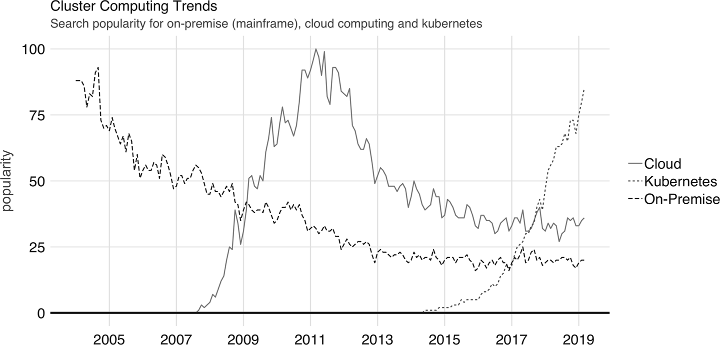
\includegraphics{figures/6_1.png}
\caption{图6-1. 内部部署(主机),云计算和Kubernetes的Google trends}
\end{figure}

在购买成百上千个计算实例时,将它们放在我们熟知的常见计算机箱中是没有意义的;相反,尽可能高效地将它们堆叠在一起以最小化使用空间是有意义的。这组高效堆叠的计算实例称为\emph{机架}。当集群增长到数千台计算机之后,你还需要托管数百个计算设备机架;在这种规模下,您还需要大量的物理空间来托管这些机架。

提供计算实例机架的建筑通常称为\emph{数据中心}。在数据中心的规模上,你还需要找到提高建筑物效率的方法,特别是冷却系统、电源、网络连接等。由于这是一项耗时的工作,一些组织以开放计算项目计划(open
Compute Project
initiative)的名义联合起来开放其基础设施的源代码,该计划为任何人免费提供一组数据中心蓝图。

没有什么可以阻止你构建自己的数据中心。事实上,许多组织都已经开始了这条道路。例如,亚马逊最初是一家在线书店,但经过几年的发展,它的销售远远不止是书。随着在线商店的增长,其数据中心的规模也在增长。2002年,亚马逊考虑把数据中心的服务器出租给公众。两年后,亚马逊网络服务(Amazon
Web
Services,AWS)推出,让任何人都可以按需租用该公司数据中心的服务器,这意味着您你需购买、配置、维护或拆除自己的集群;相反,你可以直接从AWS租下来。

这种按需计算模型就是我们今天熟知的云计算。在云中,你使用的集群不归你所有,也不在你的物理建筑中;而是由其他人拥有和管理的数据中心。今天,这个领域有许多云提供商,包括AWS、Databricks、Google、Microsoft、Qubole和许多其他公司。大多数云计算平台通过web应用程序或命令行提供用户界面来请求和管理资源。

虽然多年来在云中处理数据的好处是显而易见的,但选择一个云提供商却产生了意想不到的副作用,即把组织锁定到一个特定提供商,使得很难在提供商之间切换或返回到本地群集。201年谷歌发布的Kubernetes是一个开源系统,用于跨多个主机管理容器化应用程序。实际上,它使跨多个云提供商和本地部署变得更容易。

总而言之,我们已经看到了从本地到云计算的转变,以及最近的Kubernetes。这些技术通常被简单地描述为私有云、公共云,以及启用混合云的编排服务之一。本章将带你了解Spark和R环境中的每一种集群计算趋势。

\hypertarget{ux672cux5730ux5316}{%
\subsection{本地化}\label{ux672cux5730ux5316}}

如概述部分所述,内部部署群集代表一组由组织中的工作人员采购和管理的计算实例。这些群集可以高度定制和控制;但是,它们也可能产生较高的初始费用和维护成本。

在使用本地Spark群集时,你应该考虑两个概念:

\begin{itemize}
\tightlist
\item
  集群管理员
  与操作系统(如Windows或macOS)允许你在同一台计算机上运行多个应用程序类似,集群管理器允许多个应用程序在同一个集群中运行。在使用内部部署集群时,你需要自己选择一个。
\item
  Spark分发 虽然你可以从Apache
  Spark站点安装Spark,但是许多组织与能够为Apache
  Spark提供支持和增强的公司合作,我们通常称之为Spark分发。
\end{itemize}

\hypertarget{ux7ba1ux7406ux5668}{%
\subsubsection{管理器}\label{ux7ba1ux7406ux5668}}

要在一个计算集群上运行Spark,你需要运行能够在每一个物理机器上初始化Spark并注册所有可用计算节点的软件。这个软件就是集群管理器。Spark中可用的集群管理器包括Spark单机,YARN,Mesos和Kubernetes。

\begin{quote}
在分布式系统和集群文献中,我们经常把每一个物理机器叫做一个\emph{计算实例},\emph{计算结点}或者\emph{结点}。
\end{quote}

\hypertarget{ux5355ux673a}{%
\paragraph{单机}\label{ux5355ux673a}}

在Spark单机中,Spark使用自己作为自己的集群管理器,这允许你无需在集群中安装其他软件的情况下使用Spark。如果你计划使用集群仅运行Spark应用程序,这可能很有用;如果该集群不只用于Spark,那么像YARN、Mesos或Kubernetes这样的通用集群管理器会更适合。Spark独立文档包含有关配置、启动、监视和启用高可用性的详细信息,如图6-2所示。

由于Spark单机包含在第2章介绍的Spark安装中,你可以使用Spark安装来初始化自己机器上的本地Spark
单机集群。实际工作中,你可能希望启动不同的机器上的工作节点,但为了简单起见,我们提供了在单个机器上启动单机集群的代码。

首先,通过运行\texttt{spark\_home\_dir()}来获取\texttt{SPARK\_HOME}目录,然后按如下代码启动主节点和工作节点:

\begin{Shaded}
\begin{Highlighting}[]
\CommentTok{# Retrieve the Spark installation directory}
\NormalTok{spark_home <-}\StringTok{ }\KeywordTok{spark_home_dir}\NormalTok{()}
\CommentTok{# Build paths and classes}
\NormalTok{spark_path <-}\StringTok{ }\KeywordTok{file.path}\NormalTok{(spark_home, }\StringTok{"bin"}\NormalTok{, }\StringTok{"spark-class"}\NormalTok{)}
\CommentTok{# Start cluster manager master node}
\KeywordTok{system2}\NormalTok{(spark_path, }\StringTok{"org.apache.spark.deploy.master.Master"}\NormalTok{, }\DataTypeTok{wait =} \OtherTok{FALSE}\NormalTok{)}
\end{Highlighting}
\end{Shaded}

\begin{figure}
\centering
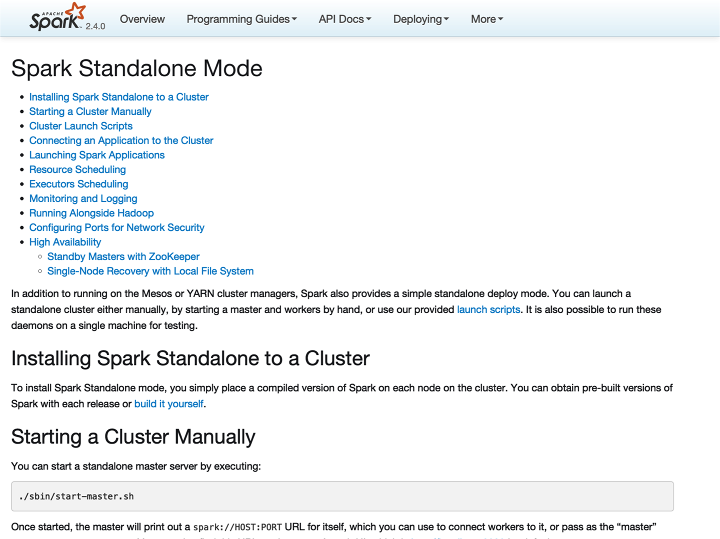
\includegraphics{figures/6_2.png}
\caption{图6-2. Spark单机网站}
\end{figure}

上一个命令初始化主节点。你可以通过localhost:8080访问主节点接口,如图6-3所示。注意,Spark主URL被指定为Spark://address:port。
你需要此URL来初始化工作节点。

然后,我们可以使用主URL初始化单个工作节点;但是,你可以使用类似的方法,即多次运行代码,在不同的机器上初始化多个工作节点:

\begin{Shaded}
\begin{Highlighting}[]
\CommentTok{# Start worker node, find master URL at http://localhost:8080/}
\KeywordTok{system2}\NormalTok{(spark_path, }\KeywordTok{c}\NormalTok{(}\StringTok{"org.apache.spark.deploy.worker.Worker"}\NormalTok{, }\StringTok{"spark://address:port"}\NormalTok{), }
    \DataTypeTok{wait =} \OtherTok{FALSE}\NormalTok{)}
\end{Highlighting}
\end{Shaded}

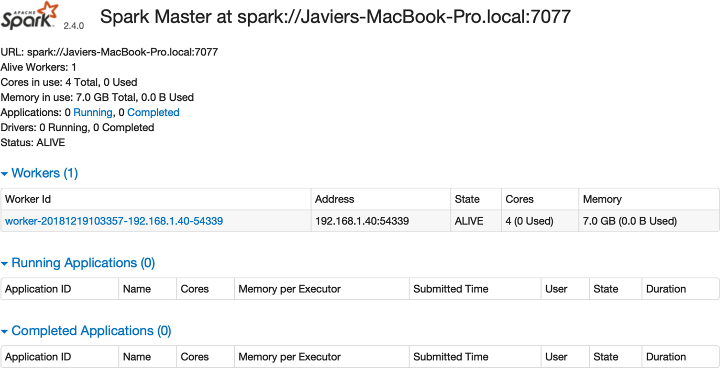
\includegraphics{figures/6_3.png}
Spark单机中只注册了一个工作节点。点击这个工作节点的链接,查看这个节点的细节,例如内存和处理器,如图6-4所示。
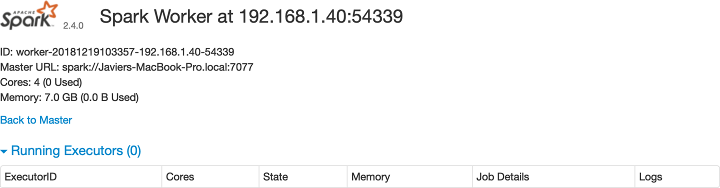
\includegraphics{figures/6_4.png}

在这个集群执行完计算之后,你需要停止主节点和工作节点。你可以使用\texttt{jps}命令来标识要终止的进程号。在下面的例子中,\texttt{15330}和\texttt{15353}是可以终止并结束集群的进程。要终止进程,可以在Windows中使用\texttt{system("Taskkill\ /PID\ \#\#\#\#\#\ /F")},在macOS或Linux中使用\texttt{system("kill\ -9\ \#\#\#\#\#")}。

\begin{Shaded}
\begin{Highlighting}[]
\KeywordTok{system}\NormalTok{(}\StringTok{"jps"}\NormalTok{)}
\DecValTok{15330}\NormalTok{ Master}
\DecValTok{15365}\NormalTok{ Jps}
\DecValTok{15353}\NormalTok{ Worker}
\DecValTok{1689}\NormalTok{ QuorumPeerMain}
\end{Highlighting}
\end{Shaded}

你可以按照类似的方法配置集群,即在集群中的每台计算机上运行初始化代码。

虽然可以初始化一个简单的单机集群,但是要配置一个合适的Spark单机集群,满足从计算机重启和故障中恢复,并且支持多个用户、权限等,通常是一更加漫长的过程。这超出了本书的范围。以下各节介绍了几种更易于在本地或通过云服务进行管理的替代方案。我们首先介绍YARN。

\hypertarget{yarn}{%
\paragraph{YARN}\label{yarn}}

Hadoop
YARN,或者简称为YARN,是Hadoop项目的资源管理器。它最初是在Hadoop项目中开发的,但在Hadoop
2中被重构为自己的项目。正如我们在第1章中提到的,Spark是为了加快Hadoop上的计算速度而构建的,因此在Hadoop集群上安装Spark很常见。

YARN的一个优点是它可能已经安装在许多支持Hadoop的现有集群上,这意味着你可以轻松地使用Spark与许多现有的Hadoop集群,而不需要对现有集群的基础设施进行任何重大改变。Spark部署在YARN集群中也非常常见,因为许多集群最初是Hadoop集群,最终也会升级支持Spark。

您可以通过两种模式提交YARN应用:YARN客户端和YARN群集。在YARN集群模式下,驱动程序(可能)正在远程运行,而在YARN客户端模式下,驱动程序在本地运行。这两种模式都支持,我们将在第7章中进一步结束它们。

YARN提供了一个资源管理用户界面,可用于访问日志、监视可用资源、终止应用程序等。从R连接到Spark后,你能够用YARN管理正在运行的应用程序,如图6-5所示。

由于YARN是Hadoop项目中的集群管理器,因此可以在Hadoop.apache.org上找到YARN的文档。你还可以参考Spark.apache.org上的````Running
Spark on YARN''指南。

\begin{figure}
\centering
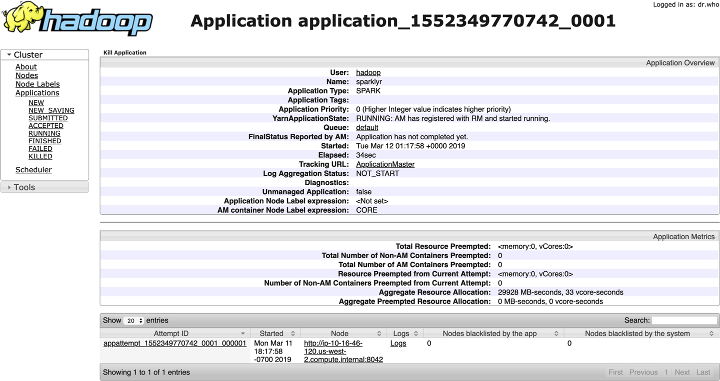
\includegraphics{figures/6_5.png}
\caption{图6-5. 运行\texttt{sparklyr}应用的YARN资源管理器}
\end{figure}

\hypertarget{apache-mesos}{%
\paragraph{Apache Mesos}\label{apache-mesos}}

Apache
Mesos是一个用于管理计算机集群的开源项目。Mesos最初是加州大学伯克利分校RAD实验室的一个研究项目,它利用Linux
Cgroup为CPU、内存、I/O和文件系统访问提供隔离。

与YARN一样,Mesos支持执行许多集群框架,包括Spark。然而,Mesos的一个优势是它允许像Spark这样的集群框架实现定制的任务调度器。调度器是集群中协调应用程序分配执行时间和资源的组件。Spark使用粗粒度的调度器,它根据应用程序的持续时间调度资源;但是,其他框架可能使用Mesos的细粒度调度器,它可以通过在较短的时间区间内调度任务来提高集群的整体效率,从而允许任务之间共享资源。

Mesos提供了一个web界面来管理正在运行的应用程序、资源等。从R连接到Spark后,你的应用程序像Mesos中运行的任何其他应用程序一样完成注册。图6-6显示了从R到Spark的成功连接。

Mesos是一个Apache项目,它的文档可以在Mesos.Apache.org上找到。如果你选择使用Mesos作为集群管理器,《Running
Spark on Mesos》指南也是一个很好的资源。

\begin{figure}
\centering
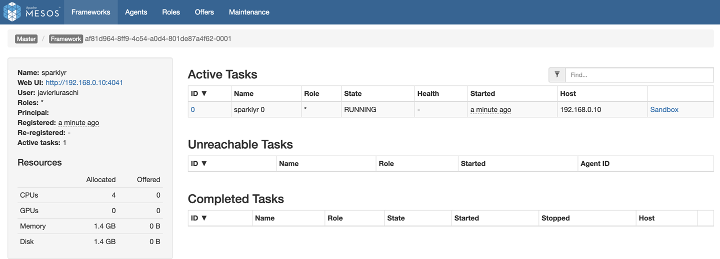
\includegraphics{figures/6_6.png}
\caption{图6-6. 运行Spark和R的Mesos网络接口}
\end{figure}

\hypertarget{ux53d1ux884cux7248}{%
\subsubsection{发行版}\label{ux53d1ux884cux7248}}

正如前一节所介绍的,你可以在本地群集中使用群集管理器;但是,许多组织(包括但不限于Apache
Spark)选择与提供附加管理软件、服务和资源的公司合作,以帮助管理其群集中的应用程序。一些本地集群提供商包括\emph{Cloudera}、\emph{Hortonworks}和\emph{MapR}。下面我们会简要介绍它们。

Cloudera,Inc.是一家美国软件公司,为商业客户提供基于Apache
Hadoop和Apache Spark的软件、支持、服务以及培训。Cloudera的混合开源Apache
Hadoop发行版,即含Apache
Hadoop的Cloudera发行版(CDH),目标成为该技术的企业级部署方案。Cloudera将其50\%以上的工程输出捐赠给Apache许可的各种开源项目(Apache
Hive、Apache Avro、Apache HBase等),这些项目结合在一起形成Apache
Hadoop平台。Cloudera也是Apache软件基金会的赞助商。

Cloudera集群使用包。包是包含程序文件和元数据的二进制发行版。Spark恰好作为一个包安装在Cloudera上。介绍如何配置Cloudera集群超出了本书的范围,但是可以在Cloudera.com和Cloudera博客上的``Introducing
sparklyr, an R Interface for Apache Spark''下找到资源和文档。

Cloudera提供Cloudera管理器网络接口来管理资源、服务、包、诊断等。图6-7显示了运行在Cloudera管理器中的Spark包,你可以稍后使用它连接R。

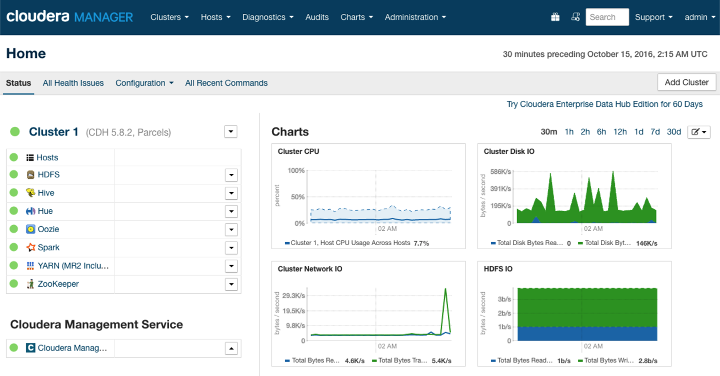
\includegraphics{figures/6_7.png}
\texttt{sparklyr}通过了Cloudera认证,意味着Cloudera也会支持\texttt{sparklyr},可以有效帮助使用Spark和R的组织。表6-1总结了当前认证的版本。

表6-1. Cloudera认证d额\texttt{sparklyr}版本

\begin{longtable}[]{@{}lllll@{}}
\toprule
Cloudera版本 & 产品 & 版本 & 构件 & Kerberos\tabularnewline
\midrule
\endhead
CDH5.9 & \texttt{sparklyr} & 0.5 & HDFS, Spark & 是\tabularnewline
CDH5.9 & \texttt{sparklyr} & 0.6 & HDFS, Spark & 是\tabularnewline
CDH5.9 & \texttt{sparklyr} & 0.7 & HDFS, Spark & 是\tabularnewline
\bottomrule
\end{longtable}

Hortonworks是一家总部位于加州圣克拉拉的大数据软件公司。公司开发、支持并提供一整套的完全开源的软件,旨在管理从物联网(IoT)到高级分析和机器学习等的数据和处理。Hortonworks相信它是一家连接云和数据中心的数据管理公司。

Hortonworks与微软合作,改善微软Windows对Hadoop和Spark的支持。这一点曾是区别于Cloudera的一个不同点;然而,自从两家公司于2019年1月合并以来,Hortonworks和Cloudera的比较在今天就不那么重要了。尽管已经合并,对Cloudera和Hortonworks的Spark发行版的支持仍然可用。在Hortonworks下配置Spark的其他资源可以在Hortonworks.com上找到。

MapR也是一家总部位于加利福尼亚州圣克拉拉的商业软件公司。MapR提供从单个计算机集群访问各种数据源的权限,包括大数据工作负载,如Apache
Hadoop和Apache
Spark,分布式文件系统,多模式数据库管理系统和事件流处理,实时分析与操作应用的结合。它的技术运行在商品硬件和公有云计算服务上。

\hypertarget{ux4e91ux7aef}{%
\subsection{云端}\label{ux4e91ux7aef}}

如果你既没有本地群集也没有备用计算机可重用,那么从云集群开始可能会非常方便,因为它允许你在几分钟内访问正确的集群。本节简要介绍了一些主要的云基础设施提供商,并提供了一些资源,帮助你在选择使用云提供商时上手。

在云服务中,计算实例的计费时间与Spark集群的运行时间一样长;当集群启动时开始计费,当集群停止时停止计费。此成本需要乘以为集群保留的实例数。因此,例如,如果一个云提供商每小时从每个计算实例收费1.00美元,而你启动一个三节点集群,使用一小时10分钟,那么你会收到1.00美元x2小时x
3节点=6.00美元的账单。
一些云提供商按分钟收费,但至少你可以采用他们每小时计算收费。

请注意,虽然小型集群的计算成本可能很低,但不经意地让集群一直运行可能会导致高额的帐单费用。因此,值得花额外的时间检查两次集群是否在不再需要时就可以终止。这也是每天使用集群时监测成本的优质实践,同时确保你的期望符合每天的账单。

根据以往的经验,在处理大型项目时,你还应该计划提前请求计算资源。但是在发出正式支持请求之前,各种云提供商不允许启动包含数百台计算机的集群。虽然这可能很麻烦,但它也是帮助你控制成本的一种方法。

由于集群的大小很灵活,从小型集群开始并按需扩展计算资源是一个很好的实践。即使你事先知道将需要一个很大规模的集群,从小规模开始也提供了一个以较低成本解决问题的机会,因为你的数据分析不太可能在第一次尝试大规模运行时毫无问题。经验法则是,以指数方式增长实例;如果需要在八节点群集上运行计算,需要从一个节点和整个数据集的八分之一开始,然后是两个节点和四分之一数据集,然后是四个节点和一半数据集,最后是八个节点和整个数据集。当你变得更有经验时,会对如何解决问题以及所需集群的大小有一个很好的了解,并且可以跳过中间步骤。但对于新手来说,这是一个很好的实践。

你还可以使用云提供商获取计算资源,然后自己安装上一节中介绍的内部部署发行版;例如,您可以在亚马逊的弹性计算云(Amazon
Elastic Compute cloud,Amazon
EC2)上运行Cloudera发行版。此模型可以避免获取同位置的硬件,但它仍然允许你密切管理和定制集群。本书只简单介绍了云提供商提供的完全托管的Spark服务。但是,你通常可以在网上轻松找到有关如何在云中安装本地发行版的说明。

云计算基础设施的主要供应商包括亚马逊、Databricks、谷歌、IBM、微软和Qubole。接下来的章节会简要介绍每一个供应商。

\hypertarget{ux4e9aux9a6cux900a}{%
\subsubsection{亚马逊}\label{ux4e9aux9a6cux900a}}

亚马逊通过AWS提供云服务。更具体的,它通过亚马逊EMR提供按需Spark集群。

使用R和亚马逊EMR的具体说明发表在Amazon的大数据博客中,名为``Running
\texttt{sparklyr} on Amazon
EMR''。这篇博文介绍了\texttt{sparklyr}的启动和通过其配置亚马逊集群的说明。例如,它推荐你可以使用亚马逊命令行界面启动三个节点的集群,代码如下:

\begin{verbatim}
aws emr create-cluster --applications Name=Hadoop Name=Spark Name=Hive \
 --release-label emr-5.8.0 --service-role EMR_DefaultRole --instance-groups \
InstanceGroupType=MASTER,InstanceCount=1,InstanceType=m3.2xlarge \
InstanceGroupType=CORE,InstanceCount=2,InstanceType=m3.2xlarge \
 --bootstrap-action Path=s3://aws-bigdata-blog/artifacts/aws-blog-emr-\
rstudio-sparklyr/rstudio_sparklyr_emr5.sh,Args=["--user-pw", "<password>", \
"--rstudio", "--arrow"] --ec2-attributes InstanceProfile=EMR_EC2_DefaultRole
\end{verbatim}

然后,你可以看到集群启动,并最终在AWS门户网站中运行,如图6-8所示。

接着,你可以导航至Master Public
DNS,并在端口8787下找到RStudio,例\texttt{如ec2-12-34-567-890.us-west-1.compute.amazonaws.com:8787},然后使用用户名\texttt{hadoop}和密码\texttt{password}登陆进入。

\begin{figure}
\centering
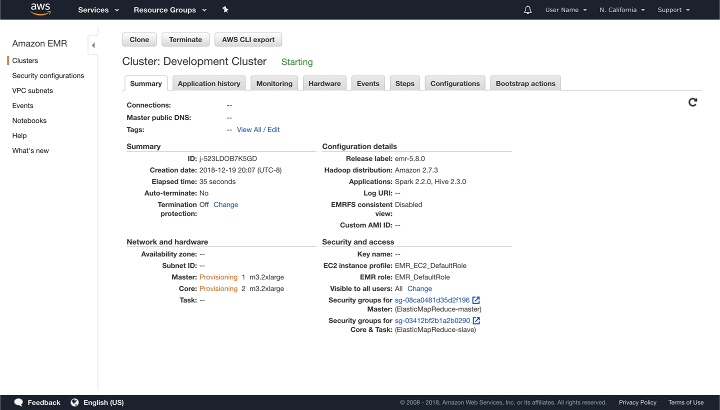
\includegraphics{figures/6_8.png}
\caption{图6-8. 启动亚马逊EMR集群}
\end{figure}

你也可以使用网络界面启动亚马逊EMR集群。同一篇介绍性博文包含专门为亚马逊EMR设计的其他详细信息和步骤。

在启动亚马逊EMR集群进行敏感数据分析时,记住关闭集群以避免不必要的费用,并使用适当的安全限制。

关于成本,你可以在Amazon EMR
Pricing上找到最新的信息。表6-2显示了\texttt{us-west-1}区域中(截至写书的时候)可用的一些实例类型;这是为了提供与云处理相关的资源和成本的简介。注意,``EMR价格是亚马逊EC2价格(底层服务器的价格)之外的价格。''

表6-2. 亚马逊EMR定价信息

\begin{longtable}[]{@{}lllllll@{}}
\toprule
实例 & CPU & 内存 & 存储 & EC2 & 成本 & EMR成本\tabularnewline
\midrule
\endhead
c1.medium & 2 & 1.7 GB & 350 GB & 0.148美元/小时 & 0.030美元/小时
&\tabularnewline
m3.2xlarge & 8 & 30 GB & 160 GB & 0.616美元/小时 & 0.140美元/小时
&\tabularnewline
i2.8xlarge & 32 & 244 GB & 6400 GB & 7.502美元/小时 & 0.270美元/小时
&\tabularnewline
\bottomrule
\end{longtable}

\begin{quote}
我们仅介绍了截至2019年亚马逊和后续云提供商提供额可用计算实例的一个子集;但是
需要注意,硬件(CPU速度、硬盘驱动器速度等)因供应商和位置而异。因此,你不能使用这些硬件表作为准确的价格比较。准确的比较需要运行特定的工作负载并考虑计算实例成本之外的其他方面。
\end{quote}

\hypertarget{databricks}{%
\subsubsection{Databricks}\label{databricks}}

Databricks是由Apache
Spark的创建者创立的一家公司,其目标是帮助客户使用Spark进行基于云的大数据处理。Databricks源于加州大学伯克利分校的AMPLab项目。

Databricks提供了企业级的集群计算套餐,以及一个免费/社区版本,用于探索功能并熟悉其环境。

启动集群后,你可以按照第2章中提供的步骤或通过在数据块上安装RStudio来使用Databricks笔记本中的R和\texttt{sparklyr}。图6-9展示了通过\texttt{sparkylyr}使用Spark的Databricks笔记本。

\begin{figure}
\centering
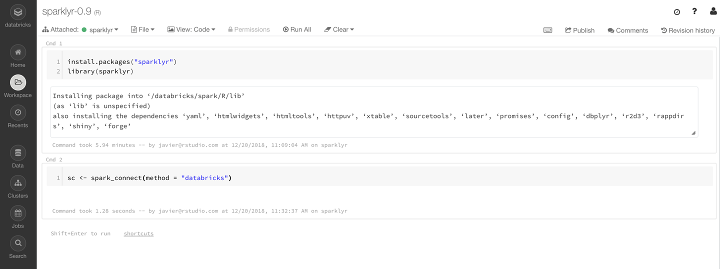
\includegraphics{figures/6_9.png}
\caption{图6-9. 运行\texttt{sparkylyr}的Databricks社区版笔记本}
\end{figure}

其他资源可以在Databricks工程博客文章``Using sparklyr in
Databricks''和\texttt{sparklyr}的Databricks文档下获得。

你可以在databricks.com/product/pricing上找到最新的定价信息。表6-3列出了截至本文撰写时可用的套餐。

表6-3. Databricks定价信息

\begin{longtable}[]{@{}llll@{}}
\toprule
套餐 & 基础定价 & 数据工程 & 数据分析\tabularnewline
\midrule
\endhead
AWS标准版 & 0.07美元/DBU & 0.20美元/DBU & 0.40美元/DBU\tabularnewline
Azure标准版 & & 0.20美元/DBU & 0.40美元/DBU\tabularnewline
Azure高级版 & & 0.35美元/DBU & 0.55美元/DBU\tabularnewline
\bottomrule
\end{longtable}

注意,定价基于每小时DBU的成本。在Databricks中,``Databricks单位(DBU)是Apache
Spark每小时处理能力的一个单位。对于一组不同的实例,DBU是一种更透明的查看使用情况的方法,而不是节点-小时。''

\hypertarget{ux8c37ux6b4c}{%
\subsubsection{谷歌}\label{ux8c37ux6b4c}}

谷歌提供谷歌云Dataproc,作为谷歌云平台(GCP)上提供的云端托管Spark和Hadoop的服务。Dataproc利用许多GCP技术,如谷歌计算引擎和g弍云存储,来提供运行主流数据处理框架(如Apache
Hadoop和Apache Spark)的完全托管集群。

你可以从谷歌云控制台或谷歌云命令行界面(CLI)轻松创建集群,如图6-10所示。

\begin{figure}
\centering
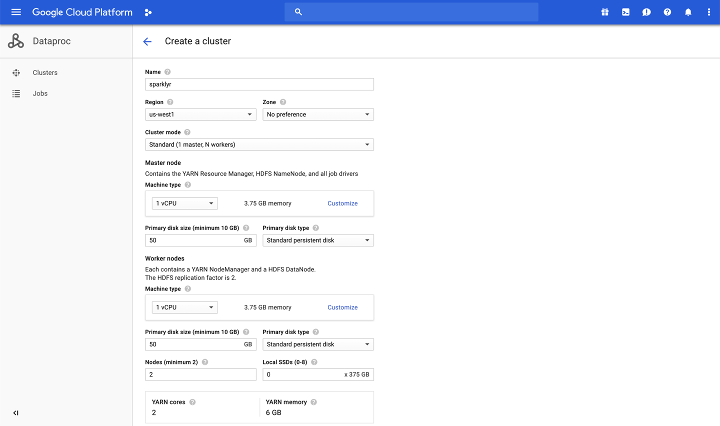
\includegraphics{figures/6_10.png}
\caption{图6-10. 启动Dataproc集群}
\end{figure}

创建集群后,可以转发端口以允许从计算机访问此集群。例如,通过启动Chrome来使用此代理并安全地连接到Dataproc集群。配置此连接,代码如下:

\begin{verbatim}
gcloud compute ssh sparklyr-m --project=<project> --zone=<region> -- -D 1080 \
 -N "<path to chrome>" --proxy-server="socks5://localhost:1080" \
 --user-data-dir="/tmp/sparklyr-m" http://sparklyr-m:8088
\end{verbatim}

有各种教程(cloud.google.com/dataproc/docs/tutorials)可以参考,包括配置RStudio和\texttt{sparklyr}的综合教程。

你可以在cloud.google.com/dataproc/pricing上找到最新的定价信息。在表6-4中,注意成本是在计算引擎和dataproc高级版之间分摊的。

Table 6-4. 谷歌云Dataproc定价信息

\begin{longtable}[]{@{}lllll@{}}
\toprule
实例e & CPU & 内存 & 计算引擎 & Dataproc高级版\tabularnewline
\midrule
\endhead
n1-standard-1 & 1 & 3.75 GB & 0.0475美元/小时 &
0.010美元/小时\tabularnewline
n1-standard-8 & 8 & 30 GB & 0.3800美元/小时 &
0.080美元/小时\tabularnewline
n1-standard-64 & 64 & 244 GB & 3.0400美元/小时 &
0.640美元/小时\tabularnewline
\bottomrule
\end{longtable}

\hypertarget{ibm}{%
\subsubsection{IBM}\label{ibm}}

IBM云计算是一套面向业务的云计算服务。IBM云包括通过公共、私有和混合云交付模型提供的基础设施即服务(IaaS)的云、软件即服务的云(SaaS)和平台即服务的云(PaaS),以及组成这些云的组件。

在IBM云服务中,打开Watson
Studio并创建一个数据科学项目,在项目设置下添加一个Spark集群,然后在Launch
IDE菜单上启动RStudio。请注意,截至写书的时候,提供的\texttt{sparklyr}版本不是CRAN中提供的最新版本,因为\texttt{sparklyr}被修改了以便IBM云下运行。在任何情况下,请按照IBM的文档作为权威参考,在IBM云上运行R和Spark,特别是如何恰当的升级\texttt{sparklyr}。图6-11展示了启动Spark集群的IBM的云门户。

\begin{figure}
\centering
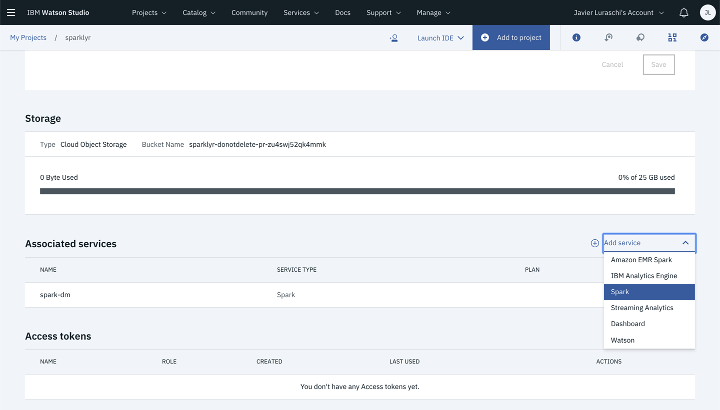
\includegraphics{figures/6_11.png}
\caption{图6-11. 使用R启动Spark集群的IBM Watson}
\end{figure}

最新的定价信息可以在ibm.com/cloud/pricing获得。在表6-5中,计算成本使用每月成本对应的31天进行了归一。

表6-5. IBM云服务定价信息

\begin{longtable}[]{@{}lllll@{}}
\toprule
实例 & CPU & 内存 & 存储 & 成本\tabularnewline
\midrule
\endhead
C1.1c1x25 & 1 & 1 GB & 25 GB & 0.033美元/小时\tabularnewline
C1.4x4x25 4 4 GB & 25 GB & 0.133美元/小时 & &\tabularnewline
C1.32x32x25 & 32 & 25 GB & 25 GB & 0.962美元/小时\tabularnewline
\bottomrule
\end{longtable}

\hypertarget{ux5faeux8f6f}{%
\subsubsection{微软}\label{ux5faeux8f6f}}

微软Azure是由微软创建的云计算服务,用于通过微软管理的数据中心全球网络来构建、测试、部署和管理应用程序和服务。它提供SaaS、PaaS和IaaS,并支持许多不同的编程语言、工具和框架,包括微软特定的和第三方软件和系统。

通过Azure门户,Azure HDInsight服务为定制化Spark集群提供支持。通过选择ML
Services集群类型,可以轻松创建支持Spark和RStudio的HDInsight集群。注意,提供的\texttt{sparklyr}版本可能不是CRAN中的最新版本,因为默认的程序包仓库似乎是使用微软R应用程序网络(MRAN)而初始化的,而不是直接从CRAN初始化的。图6-12显示了使用R启动Spark集群的Azure门户。

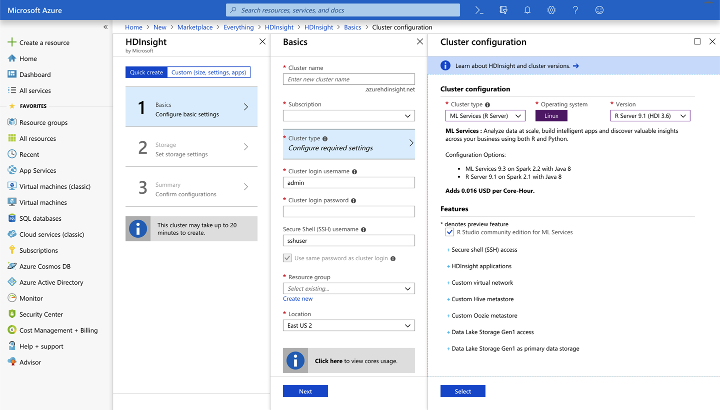
\includegraphics{figures/6_12.png}
HDInsight的最新定价信息可以在azure.microsoft.com/en-us/pricing/details/hdinsight找到。表6-6列出了写书之时的报价。

表6-6. Azure HDInsight定价信息

\begin{longtable}[]{@{}llll@{}}
\toprule
实例 & CPU & 内存 & 总成本\tabularnewline
\midrule
\endhead
D1 v2 & 1 & 3.5 GB & 0.074美元/小时\tabularnewline
D4 v2 & 8 & 28 GB & 0.59美元/小时\tabularnewline
G5 & 64 & 448 GB & 9.298美元/小时\tabularnewline
\bottomrule
\end{longtable}

\hypertarget{qubole}{%
\subsubsection{Qubole}\label{qubole}}

Qubole成立于2013年,其使命是缩小数据的可访问性差距。Qubole为基于亚马逊、微软、谷歌和甲骨文云的大数据分析提供了一个自助服务平台。在Qubole,你可以启动Spark集群,支持通过Qubole笔记本或RStudio服务器使用。图6-13展示了一个用RStudio和\texttt{sparklyr}初始化的Qubole集群。

\begin{figure}
\centering
\includegraphics{figures/6_13.png}
\caption{图6-13. 用RStudio和\texttt{sparklyr}初始化的Qubole集群}
\end{figure}

你可以在Qubole的定价页面上找到最新的定价信息。表6-7列出了截至写书的时候Qubole当前套餐的价格。注意,定价基于QCU/hr的成本,即``每小时Qubole计算单位'',而企业版本需要一份年度合同。

表6-7. Qubole定价信息

\begin{longtable}[]{@{}lll@{}}
\toprule
测试驱动 & 全功能试用版 & 企业版\tabularnewline
\midrule
\endhead
\bottomrule
\end{longtable}

0美元 0美元 0.14美元/QCU

\hypertarget{kubernetes}{%
\subsection{Kubernetes}\label{kubernetes}}

Kubernetes是一个开源的容器编排系统,用于容器化应用程序的自动部署、扩展和管理,最初由Google设计,现在由云原生计算基金会(Cloud
Native Computing
Foundation,CNCF)维护。Kubernetes最初基于Docker,而和Mesos一样,它现在也基于Linux
Cgroups。

Kubernetes可以执行许多集群应用和框架,你可以通过使用具有特定资源和库的容器镜像进行高度定制。这可以让Kubernetes集群用于数据分析之外的许多不同目的,进而又帮助组织轻松地管理他们的计算资源。使用自定义镜像需要权衡增加了进一步的配置开销的问题,但又使Kubernetes集群非常灵活。然而,这种灵活性证明,在许多组织中都有助于轻松管理集群资源。正如之前``概述''中所指出的,Kubernetes正在成为一个非常流行的集群框架。

所有主要的云提供商都支持Kubernetes。它们都提供了关于如何启动、管理和拆除Kubernetes集群的大量文档;图6-14展示了创建Kubernetes集群时的GCP控制台。你可以在任何Kubernetes集群上部署Spark,并且可以使用R来完成连接、分析、建模等操作。

\begin{figure}
\centering
\includegraphics{figures/6_14.png}
\caption{图6-14. 使用谷歌云为Spark和R创建Kubernetes集群}
\end{figure}

你可以在kubernetes.io上了解更多信息,并通过Spark.apache.org阅读《kubernetes运行Spark指南》。

严格地说,Kubernetes是一种集群技术,而不是一种特定的集群体系结构。然而,Kubernetes代表了一个更大的趋势,通常被称为混合云。混合云是一种计算环境,它利用内部部署和公有云服务,在不同平台之间进行调度。现在,要准确的对形成集群计算混合方法的主要技术进行分类还为时尚早。尽管前面提到,Kubernetes是领先的方案,但还有更多技术可能形成补充,甚至替代现有技术。

\hypertarget{ux5de5ux5177}{%
\subsection{工具}\label{ux5de5ux5177}}

虽然对于一些集群来说,仅使用R和Spark就足够了,但通常在集群中还会安装补充工具,例如分别使用Ganglia、Hue和Oozie等应用来改进监视、SQL分析、工作流协调等。本节并不打算涵盖所有工具,而是介绍常用的工具。

\hypertarget{rstudio}{%
\paragraph{RStudio}\label{rstudio}}

通过第1章的学习,你知道RStudio是R的一个著名的免费桌面开发环境;因此,很可能大家正在使用RStudio
桌面版完成本书中的示例。但是,你可能不知道RStudio也可以作为web服务在Spark集群中运行。这个版本的RStudio称为RStudio
Server。你可以在图6-15中看到正在运行的RStudio Server。与Spark
UI在集群中运行的方式相同,你可以在集群中安装RStudio
Server,然后连接到RStudio Server,并按照RStudio
Desktop完全相同的方式使用RStudio,同时支持针对Spark集群运行代码。如图6-15所示,RStudio
Server不管看起来,还是感觉起来都像RStudio
Desktop,但是它支持通过所在的集环境中来高效的运行命令。

\begin{figure}
\centering
\includegraphics{figures/6_15.png}
\caption{图6-15. 运行在AWS的RStudio Server专业版}
\end{figure}

如果你熟悉R的话,Shiny服务是从R构建交互式web应用程序的一个非常流行的工具。我们建议你直接在Spark集群中安装Shiny。

RStudio和Shiny服务器是免费开源的产品;但是,RStudio还提供RStudio
Server、RStudio Server Pro、Shiny Server Pro和RStudio
Connect等专业产品。你可以在集群内安装这些产品以支持其他R工作流程。\texttt{sparklyr}不需要任何额外的工具,但它们带来了值得考虑的生产力显著提高。你可以在rstudio.com/products/上了解更多相关信息。

\hypertarget{jupyter}{%
\paragraph{Jupyter}\label{jupyter}}

Juyter项目为开发开源软件、公开标准和跨几十种编程语言的交互式计算服务而生。Jupyter笔记本支持多种编程语言,包括R。你可以使用R内核实现\texttt{sparklyr}与Jupyter笔记本一起使用。图6-16展示了\texttt{sparklyr}在本地Jupyter笔记本中运行的情况。

\begin{figure}
\centering
\includegraphics{figures/6_16.png}
\caption{图6-16. 运行\texttt{sparklyr}的Jupyter笔记本}
\end{figure}

\hypertarget{livy}{%
\paragraph{Livy}\label{livy}}

Apache
Livy是Apache中的一个孵化项目,支持通过web界面远程使用Spark集群。直接连接到Spark集群是最理想的;但是,有时直接连接到Spark集群是不可行的。当面临这些限制时,你可以考虑在集群中安装Livy并对其进行适当的安全保护,以便能够通过web协议进行远程使用。不过,请注意,在\texttt{sparklyr}中使用Livy会带来明显的性能开销。

为了帮助在本地测试Livy,\texttt{sparklyr}通过执行\texttt{livy\_available\_versions()}列出、安装、启动和停止本地Livy实例:

\begin{Shaded}
\begin{Highlighting}[]
\CommentTok{## livy 1 0.2.0 2 0.3.0 3 0.4.0 4 0.5.0}
\end{Highlighting}
\end{Shaded}

这个命令可以列出可安装的版本。我们建议安装最新的版本并完成验证,代码如下:

\begin{Shaded}
\begin{Highlighting}[]
\CommentTok{# Install default Livy version}
\KeywordTok{livy_install}\NormalTok{()}
\DecValTok{114} \OperatorTok{|}\StringTok{ }\NormalTok{Chapter }\DecValTok{6}\OperatorTok{:}\StringTok{ }\NormalTok{Clusters}
\CommentTok{# List installed Livy services}
\KeywordTok{livy_installed_versions}\NormalTok{()}
\CommentTok{# Start the Livy service}
\KeywordTok{livy_service_start}\NormalTok{()}
\end{Highlighting}
\end{Shaded}

你可以导航至本地http://localhost:8998
上的Livy进程。第7章会具体介绍如何通过Livy连接。连接成功后,你可以导航至Livy
web应用,如图6-17所示。

\begin{figure}
\centering
\includegraphics{figures/6_17.png}
\caption{图6-17. 作为本地服务运行的Apache Livy}
\end{figure}

确保你在使用本地Livy实例的时候已经终止了Livy服务(而对于集群中运行的正常Livy服务,你无需这么做):

\begin{Shaded}
\begin{Highlighting}[]
\CommentTok{# Stops the Livy service}
\KeywordTok{livy_service_stop}\NormalTok{()}
\end{Highlighting}
\end{Shaded}

\hypertarget{ux5c0fux7ed3-4}{%
\subsection{小结}\label{ux5c0fux7ed3-4}}

本章介绍了内部部署和云计算的历史和权衡,以及Kubernetes这一提供跨内部部署或多个云提供商之间灵活性的有前途的框架。本章还引入了集群管理器(Spark
Standalone、YARN、Mesos和Kubernetes),作为运行Spark集群应用所需的软件。本章还简要介绍本地集群提供商,如Cloudera、Hortonworks和MapR,以及主要的Spark云提供商:亚马逊、Databricks、IBM、谷歌、微软和Qubole。

虽然本章为理解当前集群计算趋势、工具和服务提供商在处理大规模数据科学项目上提供了坚实的基础,但它并没有提供一个全面的框架来帮助你决定选择哪种集群技术。相反,可以将本章作为概述和起点来寻找其他资源,以帮助找到最适合组织需要的集群。

第7章将重点介绍如何连接到现有的集群,因此,就像我们在本章中介绍的,它假定Spark集群已经可用。

\begin{center}\rule{0.5\linewidth}{\linethickness}\end{center}

\hypertarget{ux7b2c7ux7ae0-ux8fdeux63a5}{%
\section{第7章 连接}\label{ux7b2c7ux7ae0-ux8fdeux63a5}}

\begin{quote}
They don't get to choose. ---Daenerys Targaryen
\end{quote}

第6章介绍了主要的集群计算趋势、集群管理器、发行版和云服务提供商,以帮助你选择最适合需要的Spark集群。相比之下,本章会介绍Spark集群内部组件以及如何连接到特定Spark集群。

阅读本章时,无需执行每一行代码。这会非常困难,因为你需要准备不同的Spark环境。相反,如果你已经有了一个Spark集群,或者上一章让你有足够的动力去注册一个按需的集群,那么现在是学习如何连接集群的时候了。本章帮助你连接到已经选择的集群。如果还没有选择集群,我们建议你学习这些概念,然后回来运行相关代码。

此外,本章还提供了各种连接故障排除技术。虽然我们不希望你需要使用它们,但还是保证你可以运用这些技术解决连接问题。

虽然本章的内容可能有点枯燥,因为连接和故障排除绝对不是大规模计算中最让人兴奋的内容,但是本章还是会介绍Spark集群的构成和交互方式,通常被称为Apache
Spark\emph{体系结构}。本章以及第8章和第9章将详细介绍Spark的工作原理,这将帮助你成长为Spark的中级用户,能够真正理解使用Apache
Spark进行分布式计算的精彩内容。

\hypertarget{ux6982ux8ff0-6}{%
\subsection{概述}\label{ux6982ux8ff0-6}}

Spark集群的所有连接体系结构由三种类型的计算实例组成:\emph{驱动节点}、\emph{工作节点}和\emph{集群管理器}。集群管理器是一种允许Spark在集群中执行的服务。这部分内容第之前的``管理器''中有详细说明。工作节点(也称为执行器)在分区数据上执行计算任务,并将中间结果传递给其他工作节点或返回给驱动节点。驱动节点的任务是将工作委托给工作节点,同时还负责聚合它们的结果和控制计算流。在大多数情况下,聚合发生在工作节点中;然而,即使在节点聚合数据之后,驱动节点通常也需要收集工作节点的结果。因此,驱动节点通常至少配备(通常更多)一些计算资源(内存、CPU、本地存储等),可以作为工作节点。

严格地说,驱动节点和工作节点只是分配了具有特定角色的机器的名称,而驱动节点中的实际计算则根据\emph{SparkContext}执行的。SparkContext是Spark功能的主要入口,因为它的任务是调度任务、管理存储、跟踪执行状态、指定访问配置的设置、取消作业等。在工作节点中,实际计算是在spark执行器下执行的,spark执行器是一个spark组件,其任务是针对特定的数据分区执行子任务。图7-1说明了这个概念,其中驱动节点通过集群管理器编排一个工作节点的工作。

\begin{figure}
\centering
\includegraphics{figures/7_1.png}
\caption{图7-1. Apache Spark连接体系结构}
\end{figure}

如果你的组织中已经有一个Spark集群,那么你应该向集群管理员请求指向该集群的连接信息,仔细阅读它们的使用策略,并遵循它们的建议。因为集群可以在许多用户之间共享,所以你需要确保只请求所需的计算资源。我们将在第9章中介绍如何请求资源。系统管理员将指定它是本地集群还是云集群、使用的集群管理器、支持的连接和支持的工具。你可以使用此信息直接跳转到本地、单机、YARN、Mesos、Livy或Kubernetes,根据这些信息可以选择适合需求的方案。

\begin{quote}
使用\texttt{spark\_connect()}连接后,可以借助\texttt{sc}连接方法使用在前面章节中描述的技术;例如,你可以使用前面章节中介绍的相同代码进行数据分析或建模。
\end{quote}

\hypertarget{ux8fb9ux7f18ux8282ux70b9}{%
\subsubsection{边缘节点}\label{ux8fb9ux7f18ux8282ux70b9}}

计算集群会完成配置,支持节点之间的大带宽和快速网络连接。为了优化网络连接,集群中的节点被配置为相互信任并禁用安全功能。这会提高性能,但需要你关闭所有外部网络通信,从而使整个集群成为一个安全的整体,只有少数集群计算机在精心配置后接受来自集群外部的连接。理论上讲,这些计算机位于集群的``边缘'',称为\emph{边缘节点}。因此,在连接到Apache
Spark之前,可能首先需要连接到集群中的边缘节点。有两种连接方法:

\begin{itemize}
\tightlist
\item
  终端 使用计算机终端应用程序,可以使用Secure
  Shell建立到集群的远程连接;连接到集群后,可以启动R,然后使用\texttt{sparklyr}。但是,终端对于一些任务,如探索性数据分析来说可能会很麻烦,因此它通常只在配置集群或故障排查时使用。
\item
  网络浏览器
  虽然可以从终端使用\texttt{sparklyr},但在边缘节点安装web服务器通常会更高效,该节点提供从网络浏览器运行R和\texttt{sparklyr}的访问权限。很可能,你会考虑使用RStudio或Jupyter,而不是从终端连接。
\end{itemize}

图7-2形象的解释了这些概念。左边部分通常是你的网络浏览器,右边部分是边缘节点。在使用网路浏览器的时候,客户端和边缘节点使用HTTP通信;在使用终端的时候,客户端和边缘节点使用Secure
Shell (SSH)通信。

\begin{figure}
\centering
\includegraphics{figures/7_2.png}
\caption{图7-2. 连接到Spark边缘节点}
\end{figure}

\hypertarget{sparkux4e3bux76eeux5f55}{%
\subsubsection{Spark主目录}\label{sparkux4e3bux76eeux5f55}}

在连接到边缘节点之后,下一步是确定Spark安装在哪里,一个名为\texttt{SPARK\_HOME}的位置。在大多数情况下,集群管理器已经将\texttt{SPARK\_HOME}环境变量设置为正确的安装路径。如果没有,你需要得到正确的\emph{SPARK\_HOME}路径。必须指定\texttt{SPARK\_HOME}路径作为环境变量,或者在运行\texttt{spark\_connect()}时显式地指定\texttt{spark\_connect()}路径。

如果你的集群提供商或集群管理员已经为提供了\emph{SPARK\_HOME},那么下面的代码应该返回路径而不是空字符串:

\begin{Shaded}
\begin{Highlighting}[]
\KeywordTok{Sys.getenv}\NormalTok{(}\StringTok{"SPARK_HOME"}\NormalTok{)}
\end{Highlighting}
\end{Shaded}

如果这段代码返回了空字符串,这就意味着集群中的\texttt{SPARK\_HOME}环境变量没有设置。所以你需要在使用\texttt{spark\_connect()}的时候指定\texttt{SPARK\_HOME},代码如下:

\begin{Shaded}
\begin{Highlighting}[]
\NormalTok{sc <-}\StringTok{ }\KeywordTok{spark_connect}\NormalTok{(}\DataTypeTok{master =} \StringTok{"master"}\NormalTok{, }\DataTypeTok{spark_home =} \StringTok{"local/path/to/spark"}\NormalTok{)}
\end{Highlighting}
\end{Shaded}

在这个例子里,设置\texttt{master},为Spark单机,YARN,Mesos,Kubernetes或Livy指向集群管理器主节点。

\hypertarget{ux672cux5730ux6a21ux5f0f}{%
\subsection{本地模式}\label{ux672cux5730ux6a21ux5f0f}}

当你以本地模式连接到Spark时,Spark会像SparkContext和单个执行一样,启动一个运行大多数集群组件的进程。这对于在大型计算集群上运行Spark、脱机工作、故障排查或测试代码非常理想。图7-3描述了Spark的本地连接。

\begin{figure}
\centering
\includegraphics{figures/7_3.png}
\caption{图7-3. 本地连接图}
\end{figure}

注意,本地模式下既没有集群管理器,也没有工作进程,因为在本地模式下,所有工作都在驱动应用程序中运行。另外值得注意的是,\texttt{sparklyr}通过\texttt{spark-submit}启动SparkContext
。\texttt{spark-submit}是每个Spark安装程序中都提供的一个脚本,允许用户向Spark提交自定义应用程序。如果你好奇的话,第13章会解释\texttt{sparklyr}中发生的提交此应用程序并从R正确连接的内部过程。

要执行本地连接,我们可以使用前面章节中熟悉的以下代码:

\begin{Shaded}
\begin{Highlighting}[]
\CommentTok{# Connect to local Spark instance}
\NormalTok{sc <-}\StringTok{ }\KeywordTok{spark_connect}\NormalTok{(}\DataTypeTok{master =} \StringTok{"local"}\NormalTok{)}
\end{Highlighting}
\end{Shaded}

\hypertarget{ux5355ux673aux6a21ux5f0f}{%
\subsection{单机模式}\label{ux5355ux673aux6a21ux5f0f}}

连接到Spark单机集群需要集群管理器主节点实例的位置。就像之前在``单机''部分介绍的,你可以在集群管理器的web界面中找到该实例。你可以通过查找以spark://开头的URL来找到此位置。

单机模式下的连接从\texttt{sparklyr}开始,它会启动\texttt{spark-submit},然后提交\texttt{sparklyr}应用程序并创建SparkContext。该Context从运行在给定主节点地址下的Spark单机实例中请求执行器。图7-4说明了此过程,这与图7-1中的总体连接架构非常相似,但有一些单机集群和\texttt{sparklyr}特有的附加细节。

\begin{figure}
\centering
\includegraphics{figures/7_4.png}
\caption{图7-4. Spark单机连接图}
\end{figure}

要完成连接,使用\texttt{spark\_connect()}中的\texttt{master\ =\ "spark://hostname:port"},代码如下:

\begin{Shaded}
\begin{Highlighting}[]
\NormalTok{sc <-}\StringTok{ }\KeywordTok{spark_connect}\NormalTok{(}\DataTypeTok{master =} \StringTok{"spark://hostname:port"}\NormalTok{)}
\end{Highlighting}
\end{Shaded}

\hypertarget{yarn-1}{%
\subsection{YARN}\label{yarn-1}}

Hadoop
YARN是Hadoop项目中的集群管理器。这是集群中最常见的集群管理器,最初是Hadoop集群;之后是和亚马逊EMR类似的Cloudera、Hortonworks和MapR发行版。YARN支持两种连接方式:YARN客户端和YARN集群。然而,YARN客户端模式比YARN集群更常见,因为它更高效,更容易建立。

\hypertarget{yarnux5ba2ux6237ux7aef}{%
\subsubsection{YARN客户端}\label{yarnux5ba2ux6237ux7aef}}

当你使用YARN客户端模式连接时,驱动实例运行R,\texttt{sparklyr}和SparkContext。这些操作需要YARN工作节点来运行Spark执行器,如图7-5所示。

\begin{figure}
\centering
\includegraphics{figures/7_5.png}
\caption{图7-5. YARN客户端连接图}
\end{figure}

要完成连接,你只需运行\texttt{master\ =\ "yarn"},代码如下:

\begin{Shaded}
\begin{Highlighting}[]
\NormalTok{sc <-}\StringTok{ }\KeywordTok{spark_connect}\NormalTok{(}\DataTypeTok{master =} \StringTok{"yarn"}\NormalTok{)}
\end{Highlighting}
\end{Shaded}

当你使用客户端模式运行YARN时,集群管理器会在后台执行你希望集群管理器执行的操作:它从集群分配资源并将它们分配给Spark应用程序。SparkContext会为你管理这些应用。在之前的的``YARN''部分中有一点需要注意,SparkContext位于运行R代码的同一台机器中;这与集群模式下运行YARN有所不同。

\hypertarget{yarnux96c6ux7fa4}{%
\subsubsection{YARN集群}\label{yarnux96c6ux7fa4}}

在集群模式下运行YARN与在客户端模式下运行YARN的主要区别在于,在集群模式下,不要求驱动节点是启动R和\texttt{sparklyr}的节点。相反,驱动节点仍然是专门指定的,通常与运行R的边缘节点不同。当边缘节点有太多并发用户、缺少计算资源或诸如RStudio或Jupyter的工具需要区别于其他集群资源管理工具进行独立管理时,考虑使用集群模式可能会有帮助。

图7-6展示了在集群模式下运行时不同组件是如何分离的。注意,仍然有一条连接客户端和集群管理器的线路,因为首先,仍然需要从集群管理器分配资源;但是,在分配资源之后,客户端直接与驱动节点通信,驱动节点与工作节点通信。从图7-6中,你可能认为集群模式看起来比客户端模式复杂得多。这种认识是正确的;因此,如果可能的话,最好避免集群模式,因为它有额外的配置开销。

\begin{figure}
\centering
\includegraphics{figures/7_6.png}
\caption{图7-6. YARN集群连接图}
\end{figure}

为了连接YARN集群节点,只需要运行下列代码:

\begin{Shaded}
\begin{Highlighting}[]
\NormalTok{sc <-}\StringTok{ }\KeywordTok{spark_connect}\NormalTok{(}\DataTypeTok{master =} \StringTok{"yarn-cluster"}\NormalTok{)}
\end{Highlighting}
\end{Shaded}

集群模式假定运行\texttt{spark\_connect()}的节点都正确配置好了,这意味着存在\texttt{yarn-site.xml},并且\texttt{YARN\_CONF\_DIR}环境变量都配置正确。。当使用Hadoop作为文件系统时,还需要\texttt{HADOOP\_CONF\_DIR}环境变量配置正确。此外,你需要确保客户端和驱动节点之间的网络连接正确,这不仅仅是需要两台机器都可以访问,而且还需要确保它们之间有足够的带宽。此配置通常由系统管理员提供,不需要手动配置。

\hypertarget{livy-1}{%
\subsection{Livy}\label{livy-1}}

与其他需要在集群中使用边缘节点的连接方法不同,Livy提供了一个web
API,使Spark集群可以从集群外部访问,并且不需要在客户端中安装Spark。在通过web
API连接之后,\emph{Livy服务}通过从集群管理器请求资源并像往常一样分发工作来启动SparkContext。图7-7展示了一个Livy连接;注意,客户端通过web
API远程连接到驱动节点。

\begin{figure}
\centering
\includegraphics{figures/7_7.png}
\caption{图7-7. Livy连接图}
\end{figure}

通过Livy连接需要指向Livy服务的URL,应该与https://hostname:port/livy类似。因为允许远程连接,连接通常至少需要基本的认证:

\begin{Shaded}
\begin{Highlighting}[]
\NormalTok{sc <-}\StringTok{ }\KeywordTok{spark_connect}\NormalTok{(}\DataTypeTok{master =} \StringTok{"https://hostname:port/livy"}\NormalTok{, }\DataTypeTok{method =} \StringTok{"livy"}\NormalTok{, }\DataTypeTok{config =} \KeywordTok{livy_config}\NormalTok{(}\DataTypeTok{spark_version =} \StringTok{"2.3.1"}\NormalTok{, }
    \DataTypeTok{username =} \StringTok{"<username>"}\NormalTok{, }\DataTypeTok{password =} \StringTok{"<password>"}\NormalTok{))}
\end{Highlighting}
\end{Shaded}

要在本地机器上使用Livy,你可以想之前在``Livy''中描述的那样,安装运行Livy服务并进行连接,代码如下:

\begin{Shaded}
\begin{Highlighting}[]
\NormalTok{sc <-}\StringTok{ }\KeywordTok{spark_connect}\NormalTok{(}\DataTypeTok{master =} \StringTok{"http://localhost:8998"}\NormalTok{, }\DataTypeTok{method =} \StringTok{"livy"}\NormalTok{, }\DataTypeTok{version =} \StringTok{"2.3.1"}\NormalTok{)}
\end{Highlighting}
\end{Shaded}

通过Livy连接后,你可以使用\texttt{sparklyr}的任何特性;但是,Livy不适合探索性数据分析,因为执行命令会带来很大的性能开销。虽然这么说,但在长时间运行计算时,这种开销可能被认为是无关紧要的。一般来说,你应该避免使用Livy并直接在集群中的边缘节点内工作;当这种策略不可行时,使用Livy才是一种合理的方法。

\begin{quote}
通过\texttt{spark\_version}参数指定Spark版本是可选的;但是,当指定了版本时,部署与给定版本兼容的预编译Java二进制文件会显著提高集群性能。因此,在使用Livy连接到Spark时,最好指定Spark版本。
\end{quote}

\hypertarget{mesos}{%
\subsection{Mesos}\label{mesos}}

与YARN类似,Mesos支持客户端模式和集群模式;但是,\texttt{sparklyr}目前仅支持Mesos下的客户端模式。因此,图7-8所示的图相当于YARN客户端图,只有集群管理器从YARN更改为Mesos。

\begin{figure}
\centering
\includegraphics{figures/7_8.png}
\caption{图7-8. Mesos连接图}
\end{figure}

连接需要指向Mesos主节点的网址。对于使用ZooKeeper的Mesos,通常形式是mesos://host:port或者mesos://zk://host1:2181,host2:2181,host3:2181/mesos。

\begin{Shaded}
\begin{Highlighting}[]
\NormalTok{sc <-}\StringTok{ }\KeywordTok{spark_connect}\NormalTok{(}\DataTypeTok{master =} \StringTok{"mesos://host:port"}\NormalTok{)}
\end{Highlighting}
\end{Shaded}

The
\texttt{MESOS\_NATIVE\_JAVA\_LIBRARY}需要经过系统管理员的设置,或者在本地机器上运行Mesos的时候手动设置。例如,在MacOS中,你可以用终端安装和初始化,然后通过手动设置Mesos库,并使用\texttt{spark\_connect()}进行连接:

\begin{verbatim}
brew install mesos
/usr/local/Cellar/mesos/1.6.1/sbin/mesos-master --registry=in_memory
 --ip=127.0.0.1 MESOS_WORK_DIR=. /usr/local/Cellar/mesos/1.6.1/sbin/mesos-slave
 --master=127.0.0.1:5050

Sys.setenv(MESOS_NATIVE_JAVA_LIBRARY =
"/usr/local/Cellar/mesos/1.6.1/lib/libmesos.dylib")
sc <- spark_connect(master = "mesos://localhost:5050",
spark_home = spark_home_dir())
\end{verbatim}

\hypertarget{kubernetes-1}{%
\subsection{Kubernetes}\label{kubernetes-1}}

Kubernetes并不像Mesos或者YARN支持客户端模式。相反,连接模型类似于YARN集集群,其中的驱动节点由Kubernetes指定,如图7-9所示。

\begin{figure}
\centering
\includegraphics{figures/7_9.png}
\caption{图7-9. Kubernetes连接图}
\end{figure}

要使用Kubernetes,你需要准备一个安装了Spark并完成正确配置的虚拟机;但是,本书不讨论如何创建一个虚拟机。完成创建后,Kubernetes连接的流程如下:

\begin{Shaded}
\begin{Highlighting}[]
\KeywordTok{library}\NormalTok{(sparklyr)}
\NormalTok{sc <-}\StringTok{ }\KeywordTok{spark_connect}\NormalTok{(}\DataTypeTok{config =} \KeywordTok{spark_config_kubernetes}\NormalTok{(}\StringTok{"k8s://https://<apiserver-host>:<apiserver-port>"}\NormalTok{, }
    \DataTypeTok{account =} \StringTok{"default"}\NormalTok{, }\DataTypeTok{image =} \StringTok{"docker.io/owner/repo:version"}\NormalTok{, }\DataTypeTok{version =} \StringTok{"2.3.1"}\NormalTok{))}
\end{Highlighting}
\end{Shaded}

如果你的计算机已经完成使用Kubernetes集群的配置,你可以使用下面的命令找出\texttt{apiserver-host}和\texttt{apiserver-port}:

\begin{Shaded}
\begin{Highlighting}[]
\KeywordTok{system2}\NormalTok{(}\StringTok{"kubectl"}\NormalTok{, }\StringTok{"cluster-info"}\NormalTok{)}
\end{Highlighting}
\end{Shaded}

\hypertarget{ux4e91ux6a21ux5f0f}{%
\subsection{云模式}\label{ux4e91ux6a21ux5f0f}}

当你使用云服务提供商时,有不同的连接方式。例如,从Databricks连接需要下面的方法:

\begin{Shaded}
\begin{Highlighting}[]
\NormalTok{sc <-}\StringTok{ }\KeywordTok{spark_connect}\NormalTok{(}\DataTypeTok{method =} \StringTok{"databricks"}\NormalTok{)}
\end{Highlighting}
\end{Shaded}

因为亚马逊EMR使用YARN,因此你可以使用\texttt{master\ =\ "yarn"}进行连接:

\begin{Shaded}
\begin{Highlighting}[]
\NormalTok{sc <-}\StringTok{ }\KeywordTok{spark_connect}\NormalTok{(}\DataTypeTok{master =} \StringTok{"yarn"}\NormalTok{)}
\end{Highlighting}
\end{Shaded}

当使用IBM的Watson
Studio连接到Spark时,需要你通过IBM提供的\texttt{load\_spark\_kernels()}函数获取一个配置对象:

\begin{Shaded}
\begin{Highlighting}[]
\NormalTok{kernels <-}\StringTok{ }\KeywordTok{load_spark_kernels}\NormalTok{()}
\NormalTok{sc <-}\StringTok{ }\KeywordTok{spark_connect}\NormalTok{(}\DataTypeTok{config =}\NormalTok{ kernels[}\DecValTok{2}\NormalTok{])}
\end{Highlighting}
\end{Shaded}

使用微软的Azure
HDInsights和ML服务(R服务器)时,Spark连接按照以下方式初始化:

\begin{Shaded}
\begin{Highlighting}[]
\KeywordTok{library}\NormalTok{(RevoScaleR)}
\NormalTok{cc <-}\StringTok{ }\KeywordTok{rxSparkConnect}\NormalTok{(}\DataTypeTok{reset =} \OtherTok{TRUE}\NormalTok{, }\DataTypeTok{interop =} \StringTok{"sparklyr"}\NormalTok{)}
\NormalTok{sc <-}\StringTok{ }\KeywordTok{rxGetSparklyrConnection}\NormalTok{(cc)}
\end{Highlighting}
\end{Shaded}

从Qubole连接需要使用\texttt{qubole}连接方法:

\begin{Shaded}
\begin{Highlighting}[]
\NormalTok{sc <-}\StringTok{ }\KeywordTok{spark_connect}\NormalTok{(}\DataTypeTok{method =} \StringTok{"qubole"}\NormalTok{)}
\end{Highlighting}
\end{Shaded}

如果需要帮助,参考你的云服务提供商文档和支持渠道。

\hypertarget{ux6279ux91cfux6a21ux5f0f}{%
\subsection{批量模式}\label{ux6279ux91cfux6a21ux5f0f}}

大多数情况下,你可以交互使用\texttt{sparklyr};也就是说,你可以显式地与\texttt{spark\_connect()}连接,然后执行命令来分析和建模大规模数据。但是,你也可以通过调度使用\texttt{sparklyr}的spark作业来自动化进程。Spark不提供调度数据处理任务的工具;相反,你要使用其他工作流管理工具。这对于转换数据、准备模型和隔夜数据打分,或者其他系统使用Spark非常有用。

例如,你可以创建名为\texttt{batch.R}的文件,其中包含以下内容:

\begin{Shaded}
\begin{Highlighting}[]
\KeywordTok{library}\NormalTok{(sparklyr)}
\NormalTok{sc <-}\StringTok{ }\KeywordTok{spark_connect}\NormalTok{(}\DataTypeTok{master =} \StringTok{"local"}\NormalTok{)}
\KeywordTok{sdf_len}\NormalTok{(sc, }\DecValTok{10}\NormalTok{) }\OperatorTok\StringTok{ }\KeywordTok{spark_write_csv}\NormalTok{(}\StringTok{"batch.csv"}\NormalTok{)}
\KeywordTok{spark_disconnect}\NormalTok{(sc)}
\end{Highlighting}
\end{Shaded}

然后,你可以使用\texttt{spark\_submit()}给Spark提交这个申请。\texttt{master}参数应该完成设置:

\begin{Shaded}
\begin{Highlighting}[]
\KeywordTok{spark_submit}\NormalTok{(}\DataTypeTok{master =} \StringTok{"local"}\NormalTok{, }\StringTok{"batch.R"}\NormalTok{)}
\end{Highlighting}
\end{Shaded}

你也可以从Shell直接调用\texttt{spark-submit}代码如下:

\begin{Shaded}
\begin{Highlighting}[]
\OperatorTok{/}\NormalTok{spark}\OperatorTok{-}\NormalTok{home}\OperatorTok{-}\NormalTok{path}\OperatorTok{/}\NormalTok{spark}\OperatorTok{-}\NormalTok{submit}
 \OperatorTok{--}\NormalTok{class }\StringTok{`}\DataTypeTok{sparklyr}\StringTok{`}\NormalTok{.Shell }\StringTok{'/spark-jars-path/sparklyr-2.3-2.11.jar'}
\DecValTok{8880} \DecValTok{12345} \OperatorTok{--}\NormalTok{batch }\OperatorTok{/}\NormalTok{path}\OperatorTok{/}\NormalTok{to}\OperatorTok{/}\NormalTok{batch.R}
\end{Highlighting}
\end{Shaded}

最后一个参数表示端口号8880和进程号12345。你可以将其设置为任何唯一的数字标识符。使用以下R代码获得正确的路径:

\begin{Shaded}
\begin{Highlighting}[]
\CommentTok{# Retrieve spark-home-path}
\KeywordTok{spark_home_dir}\NormalTok{()}
\CommentTok{# Retrieve spark-jars-path}
\KeywordTok{system.file}\NormalTok{(}\StringTok{"java"}\NormalTok{, }\DataTypeTok{package =} \StringTok{"sparklyr"}\NormalTok{)}
\end{Highlighting}
\end{Shaded}

你可以通过给\texttt{spark\_submit()}传递额外的命令行参数定制你的脚本,并使用R的\texttt{commandArgs()}读取出来。

\hypertarget{ux5de5ux5177-1}{%
\subsection{工具}\label{ux5de5ux5177-1}}

使用Jupyter和RStudio等工具连接到Spark集群时,你可以运行本章中介绍的相同连接参数。但是,由于许多云提供商使用web代理来保护Spark的web界面,要使用\texttt{spark\_web()}或RStudio
Connections窗口扩展,你需要正确配置\texttt{sparklyr.web.spark},然后通过\texttt{config}参数将其传递给\texttt{spark\_config()}。

例如,在使用亚马逊EMR时,可以通过动态检索YARN应用程序和构建EMR代理URL来配置\texttt{sparklyr.web.spark}和\texttt{sparklyr.web.yarn}:

\begin{Shaded}
\begin{Highlighting}[]
\NormalTok{domain <-}\StringTok{ "http://ec2-12-345-678-9.us-west-2.compute.amazonaws.com"}
\NormalTok{config <-}\StringTok{ }\KeywordTok{spark_config}\NormalTok{()}
\NormalTok{config}\OperatorTok{$}\NormalTok{sparklyr.web.spark <-}\StringTok{ }\ErrorTok{~}\KeywordTok{paste0}\NormalTok{(domain, }\StringTok{":20888/proxy/"}\NormalTok{, }\KeywordTok{invoke}\NormalTok{(}\KeywordTok{spark_context}\NormalTok{(sc), }
    \StringTok{"applicationId"}\NormalTok{))}
\NormalTok{config}\OperatorTok{$}\NormalTok{sparklyr.web.yarn <-}\StringTok{ }\KeywordTok{paste0}\NormalTok{(domain, }\StringTok{":8088"}\NormalTok{)}
\NormalTok{sc <-}\StringTok{ }\KeywordTok{spark_connect}\NormalTok{(}\DataTypeTok{master =} \StringTok{"yarn"}\NormalTok{, }\DataTypeTok{config =}\NormalTok{ config)}
\end{Highlighting}
\end{Shaded}

\hypertarget{ux591aux6b21ux8fdeux63a5}{%
\subsection{多次连接}\label{ux591aux6b21ux8fdeux63a5}}

通常,我们只会连接Spark一次,而且只有一次。但是,你也可以通过连接到不同的集群或指定\texttt{app\_name}参数来打开多次Spark连接。这有助于在提交到集群之前比较Spark版本或验证你的分析结果。以下示例打开了与Spark
1.6.3、2.3.0和Spark单击的连接:

\begin{Shaded}
\begin{Highlighting}[]
\CommentTok{# Connect to local Spark 1.6.3}
\NormalTok{sc_}\DecValTok{16}\NormalTok{ <-}\StringTok{ }\KeywordTok{spark_connect}\NormalTok{(}\DataTypeTok{master =} \StringTok{"local"}\NormalTok{, }\DataTypeTok{version =} \StringTok{"1.6"}\NormalTok{)}
\CommentTok{# Connect to local Spark 2.3.0}
\NormalTok{sc_}\DecValTok{23}\NormalTok{ <-}\StringTok{ }\KeywordTok{spark_connect}\NormalTok{(}\DataTypeTok{master =} \StringTok{"local"}\NormalTok{, }\DataTypeTok{version =} \StringTok{"2.3"}\NormalTok{, }\DataTypeTok{appName =} \StringTok{"Spark23"}\NormalTok{)}
\CommentTok{# Connect to local Spark Standalone}
\NormalTok{sc_standalone <-}\StringTok{ }\KeywordTok{spark_connect}\NormalTok{(}\DataTypeTok{master =} \StringTok{"spark://host:port"}\NormalTok{)}
\end{Highlighting}
\end{Shaded}

最后,你可以断开每个连接:

\begin{Shaded}
\begin{Highlighting}[]
\KeywordTok{spark_disconnect}\NormalTok{(sc_}\DecValTok{1}\NormalTok{_}\DecValTok{6}\NormalTok{_}\DecValTok{3}\NormalTok{)}
\KeywordTok{spark_disconnect}\NormalTok{(sc_}\DecValTok{2}\NormalTok{_}\DecValTok{3}\NormalTok{_}\DecValTok{0}\NormalTok{)}
\KeywordTok{spark_disconnect}\NormalTok{(sc_standalone)}
\end{Highlighting}
\end{Shaded}

你也可以一次性断开所有连接:

\begin{Shaded}
\begin{Highlighting}[]
\KeywordTok{spark_disconnect_all}\NormalTok{()}
\end{Highlighting}
\end{Shaded}

\hypertarget{ux6545ux969cux6392ux9664}{%
\subsection{故障排除}\label{ux6545ux969cux6392ux9664}}

最后,我们介绍以下故障排除技术:日志记录、Spark
Submit和Windows。如果不确定从何处开始,请在使用Windows系统时从Windows部分开始,然后是日志记录,最后是Spark
Submit。当运行\texttt{spark\_connect()}失败并显示错误消息时,这些技术非常有用。

\hypertarget{ux8bb0ux5f55ux65e5ux5fd7}{%
\subsubsection{记录日志}\label{ux8bb0ux5f55ux65e5ux5fd7}}

第一项故障排除技术是直接打印Spark日志到控制台,帮助你定位额外的错误消息:

\begin{Shaded}
\begin{Highlighting}[]
\NormalTok{sc <-}\StringTok{ }\KeywordTok{spark_connect}\NormalTok{(}\DataTypeTok{master =} \StringTok{"local"}\NormalTok{, }\DataTypeTok{log =} \StringTok{"console"}\NormalTok{)}
\end{Highlighting}
\end{Shaded}

另外,你可以通过设定连接时\texttt{sparklyr.verbose}选项为\texttt{TRUE}来开启详细日志:

\begin{Shaded}
\begin{Highlighting}[]
\NormalTok{sc <-}\StringTok{ }\KeywordTok{spark_connect}\NormalTok{(}\DataTypeTok{master =} \StringTok{"local"}\NormalTok{, }\DataTypeTok{log =} \StringTok{"console"}\NormalTok{, }\DataTypeTok{config =} \KeywordTok{list}\NormalTok{(}\DataTypeTok{sparklyr.verbose =} \OtherTok{TRUE}\NormalTok{))}
\end{Highlighting}
\end{Shaded}

\hypertarget{spark-submit}{%
\subsubsection{Spark Submit}\label{spark-submit}}

通常,你可以通过\texttt{spark\_submit()}运行一个示例任务,判断一个连接问题是R导致的还是Spark导致的,并说明没有抛出错误:

\begin{Shaded}
\begin{Highlighting}[]
\CommentTok{# Find the spark directory using an environment variable}
\NormalTok{spark_home <-}\StringTok{ }\KeywordTok{Sys.getenv}\NormalTok{(}\StringTok{"SPARK_HOME"}\NormalTok{)}
\CommentTok{# Or by getting the local spark installation}
\NormalTok{spark_home <-}\StringTok{ }\NormalTok{sparklyr}\OperatorTok{::}\KeywordTok{spark_home_dir}\NormalTok{()}
\end{Highlighting}
\end{Shaded}

然后,使用故障排除中正确的\texttt{master}参数替换\texttt{"local"}计算圆周率例子:

\begin{Shaded}
\begin{Highlighting}[]
\CommentTok{# Launching a sample application to compute Pi}
\KeywordTok{system2}\NormalTok{(}
\KeywordTok{file.path}\NormalTok{(spark_home, }\StringTok{"bin"}\NormalTok{, }\StringTok{"spark-submit"}\NormalTok{),}
\KeywordTok{c}\NormalTok{(}
\StringTok{"--master"}\NormalTok{, }\StringTok{"local"}\NormalTok{,}
\StringTok{"--class"}\NormalTok{, }\StringTok{"org.apache.spark.examples.SparkPi"}\NormalTok{,}
\KeywordTok{dir}\NormalTok{(}\KeywordTok{file.path}\NormalTok{(spark_home, }\StringTok{"examples"}\NormalTok{, }\StringTok{"jars"}\NormalTok{),}
\DataTypeTok{pattern =} \StringTok{"spark-examples"}\NormalTok{, }\DataTypeTok{full.names =} \OtherTok{TRUE}\NormalTok{),}
\DecValTok{100}\NormalTok{),}
\DataTypeTok{stderr =} \OtherTok{FALSE}
\NormalTok{)}
\NormalTok{Pi is roughly }\FloatTok{3.1415503141550314}
\end{Highlighting}
\end{Shaded}

如果前面的消息没有显示,你需要调查为什么您的Spark集群没有正确配置。这超出了本书的范围。首先,重新运行圆周率例子,但是要删除\texttt{stderr\ =\ FALSE};这会将错误消息打印到控制台,然后你可以使用控制台的消息来调查问题可能的原因。当使用云提供商或Spark发行版时,你可以联系他们的支持团队帮助进一步解决此问题;另外,Stack
Overflow也是一个很好的调查问题的起点。如果你确实看到消息,这意味着你的Spark群集已正确配置,但是不知道为什么故R无法使用Spark,因此你还需要详细地解决此问题,我们接下来会解释。

\hypertarget{ux6545ux969cux6392ux9664ux7ec6ux8282}{%
\paragraph{故障排除细节}\label{ux6545ux969cux6392ux9664ux7ec6ux8282}}

要详细排除连接过程的故障,可以手动复制两步连接过程,这通常对诊断连接问题非常有帮助。首先,从R调用\texttt{spark\_submit()},将应用提交给spark;其次,R连接到正在运行的spark应用程序。

首先,通过运行以下命令来标识Spark安装目录和正确\texttt{sparklyr*.jar}文件路径:

\begin{Shaded}
\begin{Highlighting}[]
\KeywordTok{dir}\NormalTok{(}\KeywordTok{system.file}\NormalTok{(}\StringTok{"java"}\NormalTok{, }\DataTypeTok{package =} \StringTok{"sparklyr"}\NormalTok{), }\DataTypeTok{pattern =} \StringTok{"sparklyr"}\NormalTok{, }\DataTypeTok{full.names =}\NormalTok{ T)}
\end{Highlighting}
\end{Shaded}

确保你找到了匹配Saprk的正确版本。例如,\texttt{sparklyr-2.1-2.11.jar}匹配Spark
2.1。

然后,在终端中运行以下代码:

\begin{verbatim}
$SPARK_HOME/bin/spark-submit --class `sparklyr`。Shell $PATH_TO_SPARKLYR_JAR 8880 42
18/06/11 12:13:53 INFO sparklyr: Session (42) found port 8880 is available
18/06/11 12:13:53 INFO sparklyr: Gateway (42) is waiting for `sparklyr` client
 to connect to port 8880
\end{verbatim}

参数8880表示\texttt{sparklyr}中使用的默认端口,而42是进程号,这是\texttt{sparklyr}生成的加密安全号,但出于故障排除的目的,可以简化为42。

如果第一个连接步骤失败,这意味着集群无法接受应用程序。这通常意味着没有足够的资源,或者存在权限限制。

第二步是按如下方式从R连接(注意有60秒的超时,在运行终端命令后需要运行R命令;如果需要,你可以按照第9章中的说明配置超时参数):

\begin{Shaded}
\begin{Highlighting}[]
\KeywordTok{library}\NormalTok{(sparklyr)}
\NormalTok{sc <-}\StringTok{ }\KeywordTok{spark_connect}\NormalTok{(}\DataTypeTok{master =} \StringTok{"sparklyr://localhost:8880/42"}\NormalTok{, }\DataTypeTok{version =} \StringTok{"2.3"}\NormalTok{)}
\end{Highlighting}
\end{Shaded}

如果第二个连接步骤失败,通常意味着R和驱动节点之间存在连接问题。例如,你可以尝试使用其他连接端口。

\hypertarget{windows}{%
\subsubsection{Windows}\label{windows}}

在大多数情况下,Windows连接和从Linux和macOS连接一样简单。但是,有几个常见的连接问题需要注意:

\begin{itemize}
\tightlist
\item
  防火墙和防病毒软件可能会阻止连接端口。\texttt{sparklyr}使用的默认端口是8880;请仔细检查此端口是否未被阻止。
\item
  长路径名可能会导致问题,特别是对于像Windows
  7这样的旧Windows系统。使用这些系统时,请尝试与所有文件夹一起安装的Spark连接,最多使用8个字符,名称中不要有空格。
\end{itemize}

\hypertarget{ux5c0fux7ed3-5}{%
\subsection{小结}\label{ux5c0fux7ed3-5}}

本章介绍了Spark的体系结构、连接概念和在本地模式、单机模式、YARN模式、Mesos模式、Kubernetes模式和Livy模式下连接的示例,并介绍了边缘节点及其在连接到Spark集群时的作用。这些内容应该可以给你提供足够的信息,以便成功连接到任何Apache
Spark集群。

要解决本章介绍的技术之外的连接问题,我们建议你在Stack
Overflow、\texttt{sparklyr}问题的GitHub页面中搜索连接问题。如果需要,在\texttt{sparklyr}中打开一个新的GitHub问题以进一步获得帮助。

在第8章中,我们会介绍如何使用Spark读写来自从各种数据源和格式的数据,这可以让你在数据分析时更加灵活的添加新的数据源。过去需要几天,几周,甚至几个月完成的事情,现在你可以通过拥抱数据湖在数小时内完成。

\begin{center}\rule{0.5\linewidth}{\linethickness}\end{center}

\hypertarget{ux7b2c8ux7ae0-ux6570ux636e}{%
\section{第8章 数据}\label{ux7b2c8ux7ae0-ux6570ux636e}}

\begin{quote}
Has it occurred to you that she might not have been a reliable source of
information? ---Jon Snow
\end{quote}

根据前面章节中获得的知识,你现在可以进行大规模数据分析和建模了!然而,到目前为止,我们还没有真正解释过如何将数据读入Spark。我们已经探索了如何使用\texttt{copy\_to()}上传小数据集或使用函数,如\texttt{spark\_read\_csv()}或
\texttt{spark\_write\_csv()},但没有详细解释过程和原因。

所以,你会学习到如何使用Spark读写数据。尽管这一点很重要,但本章还会向介绍数据湖------按照自然或原始格式存储的数据仓库,它提供了有别于现有存储体系结构的优点。例如,你可以轻松地集成来自外部系统的数据,而无需将其转换为通用格式,也无需假定这些源与内部数据源一样可靠。

此外,我们还将讨论如何扩展Spark的能力,使其能够处理无法直接访问的数据,并提出一些提高数据读写性能建议。读取大型数据集通常需要微调Spark集群配置,但这是第9章的主题。

\hypertarget{ux6982ux8ff0-7}{%
\subsection{概述}\label{ux6982ux8ff0-7}}

在第1章中,你学习到除了大数据和大计算之外,还可以使用Spark来提高数据任务的速度、多样性和准确性。虽然你可以将本章的知识用于任何需要加载和存储数据的任务中,但在处理各种数据源的时,本章的内容尤其有趣。为了理解原因,我们首先应该快速看一下,当今数据在许多组织中是如何处理的。

多年来,人们经常把大型数据集存储在关系\emph{数据库}中,这是Edgar
F.Codd于1970年首次提出的一种系统\footnote{Codd EF (1970). ``A relational
  model of data for large shared data banks.''}。你可以将数据库视为相互关联的表的集合,其中每个表都经过精心设计以保存特定的数据类型和与其他表的关系。大多数关系数据库系统使用\emph{结构化查询语言(Structured
Query
Language,SQL)}来查询和维护数据库。数据库在今天仍然被广泛使用,这是有充分理由的:它们可靠且一致地存储数据;事实上,你的银行很可会将帐户余额存储在数据库中,这是一种很好的实践。

然而,数据库也被用来存储来自其他应用程序和系统的信息。例如,你的银行还可能存储其他银行生成的数据,例如传入的支票。要做到这一点,需要从外部系统中提取外部数据,转换成适合当前数据库的数据,最后加载到数据库。这称为\emph{提取}、\emph{转换}和\emph{加载}(ETL),是一种将数据从一个或多个源复制到目标系统的通用过程,该目标系统以不同于源的方式表示数据。ETL过程从20世纪70年代开始流行。

除了数据库之外,数据通常还加载到\emph{数据仓库}中,数据仓库是一个用于报告和数据分析的系统。数据通常以提高数据分析速度的格式存储和索引,但这种格式通常不适合建模或运行自定义的分布式代码。挑战在于,更改数据库和数据仓库通常是一个漫长而微妙的过程,因为需要重新建立数据索引,并且需要小心地将来自多个数据源的数据转换为单个跨数据源共享的表。

不要试图将所有数据源转换为通用格式,你可以在一个数据湖、即一个以其自然格式存储的数据系统或存储库中包含各种数据源(见图8-1)。由于数据湖允许使数据以其原始格式存储,所以不必预先对其进行仔细的转换,任何人都可以使用它进行分析,这就大大增加了ETL的灵活性。然后,你可以使用Spark通过一个可在所有数据池、数据库和数据仓库中扩展的单一接口来统一数据处理。一些组织还使用Spark替换现有ETL过程;然而,这属于数据工程领域,远远超出了这本书的范围。我们在图8-1中用虚线来说明这一点。

\begin{figure}
\centering
\includegraphics{figures/8_1.png}
\caption{图8-1. Spark处理来自数据湖,数据库和数据仓库的原始数据}
\end{figure}

为了支持各种各样的数据源,Spark需要能够读写几种不同的文件格式(CSV、JSON、Parquet和其他格式),并访问存储在几个文件系统(HDFS、S3、DBFS等)中的数据,并且可能与其他存储系统(数据库、数据仓库等)进行交互。我们会讨论所有这些内容,但首先,我们会介绍如何使用Spark读取、写入和复制数据。

\hypertarget{ux8bfbux53d6ux6570ux636e}{%
\subsection{读取数据}\label{ux8bfbux53d6ux6570ux636e}}

如果你是Spark新手,强烈建议你在开始使用大型数据集之前查阅本节。我们将介绍几种提高数据读取速度和效率的技术。每个子章节都介绍了利用Spark读取文件的具体方法,例如可以将整个文件夹视为数据集,以及可以描述数据集以便在Spark中更快地读取。

\hypertarget{ux8defux5f84}{%
\subsubsection{路径}\label{ux8defux5f84}}

在分析数据时,通常将多个文件加载到单个数据对象中。在R中,我们通常使用循环或函数式编程指令来实现这一点。这是因为R必须单独加载每个文件传递到R进程中。让我们在文件夹中创建几个CSV文件,并先用R进行读取:

\begin{Shaded}
\begin{Highlighting}[]
\NormalTok{letters <-}\StringTok{ }\KeywordTok{data.frame}\NormalTok{(}\DataTypeTok{x =}\NormalTok{ letters, }\DataTypeTok{y =} \DecValTok{1}\OperatorTok{:}\KeywordTok{length}\NormalTok{(letters))}
\KeywordTok{dir.create}\NormalTok{(}\StringTok{"data-csv"}\NormalTok{)}
\KeywordTok{write.csv}\NormalTok{(letters[}\DecValTok{1}\OperatorTok{:}\DecValTok{3}\NormalTok{, ], }\StringTok{"data-csv/letters1.csv"}\NormalTok{, }\DataTypeTok{row.names =} \OtherTok{FALSE}\NormalTok{)}
\KeywordTok{write.csv}\NormalTok{(letters[}\DecValTok{1}\OperatorTok{:}\DecValTok{3}\NormalTok{, ], }\StringTok{"data-csv/letters2.csv"}\NormalTok{, }\DataTypeTok{row.names =} \OtherTok{FALSE}\NormalTok{)}
\KeywordTok{do.call}\NormalTok{(}\StringTok{"rbind"}\NormalTok{, }\KeywordTok{lapply}\NormalTok{(}\KeywordTok{dir}\NormalTok{(}\StringTok{"data-csv"}\NormalTok{, }\DataTypeTok{full.names =} \OtherTok{TRUE}\NormalTok{), read.csv))}
\NormalTok{ x y}
\DecValTok{1}\NormalTok{ a }\DecValTok{1}
\DecValTok{2}\NormalTok{ b }\DecValTok{2}
\DecValTok{3}\NormalTok{ c }\DecValTok{3}
\DecValTok{4}\NormalTok{ a }\DecValTok{1}
\DecValTok{5}\NormalTok{ b }\DecValTok{2}
\DecValTok{6}\NormalTok{ c }\DecValTok{3}
\end{Highlighting}
\end{Shaded}

在Spark中,将一个文件夹作为数据集是一个重要的思想。我们只需传递包含所有文件的路径就可以,而不是枚举每个文件。Spark假设该文件夹中的每个文件都是同一数据集的一部分。这意味着目标文件夹只能用于数据目的。这一点尤其重要,因为像HDFS这样的存储系统会存储跨多台计算机的文件,但从概念上讲,它们存储在同一个文件夹中;当Spark从这个文件夹中读取文件时,实际上是执行分布式代码来读取每台计算机中的每个文件。当读取分布式文件的时候,并没有数据转移:

\begin{Shaded}
\begin{Highlighting}[]
\KeywordTok{library}\NormalTok{(sparklyr)}
\NormalTok{sc <-}\StringTok{ }\KeywordTok{spark_connect}\NormalTok{(}\DataTypeTok{master =} \StringTok{"local"}\NormalTok{, }\DataTypeTok{version =} \StringTok{"2.3"}\NormalTok{)}
\KeywordTok{spark_read_csv}\NormalTok{(sc, }\StringTok{"data-csv/"}\NormalTok{)}
\CommentTok{# Source: spark<datacsv> [?? x 2]}
\NormalTok{ x y}
 \OperatorTok{<}\NormalTok{chr}\OperatorTok{>}\StringTok{ }\ErrorTok{<}\NormalTok{int}\OperatorTok{>}
\StringTok{ }\DecValTok{1}\NormalTok{ a }\DecValTok{1}
 \DecValTok{2}\NormalTok{ b }\DecValTok{2}
 \DecValTok{3}\NormalTok{ c }\DecValTok{3}
 \DecValTok{4}\NormalTok{ d }\DecValTok{4}
 \DecValTok{5}\NormalTok{ e }\DecValTok{5}
 \DecValTok{6}\NormalTok{ a }\DecValTok{1}
 \DecValTok{7}\NormalTok{ b }\DecValTok{2}
 \DecValTok{8}\NormalTok{ c }\DecValTok{3}
 \DecValTok{9}\NormalTok{ d }\DecValTok{4}
\DecValTok{10}\NormalTok{ e }\DecValTok{5}
\end{Highlighting}
\end{Shaded}

``文件夹即表''的思想也可以在其他开源技术中找到。Hive表的后台工作原理是一样的。当你查询一个Hive表时,映射会在同一文件夹中的多个文件上完成。文件夹的名称通常与用户可见的表的名称匹配。

接下来,我们会介绍一种技术,它允许Spark更快地读取文件,并通过预先描述数据集的结构来避免读取失败。

\hypertarget{ux6a21ux5f0f}{%
\subsubsection{模式}\label{ux6a21ux5f0f}}

在读取数据时,Spark能够确定数据源的列名和列类型,也称为模式。然而,猜测模式是有代价的;Spark需要初步传递一些数据来猜测它是什么。对于大型数据集,这会给数据读取过程增加大量时间,即使对于中等大小的数据集,这也会增加成本。对于反复读取的文件,额外的读取时间会随着时间的推移而累积。

为了避免这种情况,Spark允许通过提供一个\texttt{columns}参数定义列,来描述数据集。你自己可以对原始文件的一小部分进行采样来创建这个模式:

\begin{Shaded}
\begin{Highlighting}[]
\NormalTok{spec_with_r <-}\StringTok{ }\KeywordTok{sapply}\NormalTok{(}\KeywordTok{read.csv}\NormalTok{(}\StringTok{"data-csv/letters1.csv"}\NormalTok{, }\DataTypeTok{nrows =} \DecValTok{10}\NormalTok{), class)}
\NormalTok{spec_with_r}
\NormalTok{ x y}
 \StringTok{"factor"} \StringTok{"integer"}
\end{Highlighting}
\end{Shaded}

你也可以把列的说明来设置为一个显式包含列类型的向量。这个向量的值按照与字段名匹配的方式命名:

\begin{Shaded}
\begin{Highlighting}[]
\NormalTok{spec_explicit <-}\StringTok{ }\KeywordTok{c}\NormalTok{(}\DataTypeTok{x =} \StringTok{"character"}\NormalTok{, }\DataTypeTok{y =} \StringTok{"numeric"}\NormalTok{)}
\NormalTok{spec_explicit}
\NormalTok{ x y}
\StringTok{"character"} \StringTok{"numeric"}
\end{Highlighting}
\end{Shaded}

可接受的变量类型有:\texttt{integer},\texttt{character},\texttt{logical},\texttt{double},\texttt{numeric},\texttt{factor},\texttt{Date}和
\texttt{POSIXct}。

然后,在使用\texttt{spark\_read\_csv()}读取时,可以\texttt{spec\_with\_r}传递给\texttt{columns}参数,以匹配原始文件的名称和类型。这有助于提高性能,因为Spark不需要确定列类型。

\begin{Shaded}
\begin{Highlighting}[]
\KeywordTok{spark_read_csv}\NormalTok{(sc, }\StringTok{"data-csv/"}\NormalTok{, }\DataTypeTok{columns =}\NormalTok{ spec_with_r)}
\CommentTok{# Source: spark<datacsv> [?? x 2]}
\NormalTok{ x y}
 \OperatorTok{<}\NormalTok{chr}\OperatorTok{>}\StringTok{ }\ErrorTok{<}\NormalTok{int}\OperatorTok{>}
\DecValTok{1}\NormalTok{ a }\DecValTok{1}
\DecValTok{2}\NormalTok{ b }\DecValTok{2}
\DecValTok{3}\NormalTok{ c }\DecValTok{3}
\DecValTok{4}\NormalTok{ a }\DecValTok{1}
\DecValTok{5}\NormalTok{ b }\DecValTok{2}
\DecValTok{6}\NormalTok{ c }\DecValTok{3}
\end{Highlighting}
\end{Shaded}

下面的示例演示如何将字段类型设置为不同的类型。新的字段类型需要与原始数据集兼容。例如,不能将\texttt{character}字段设置为\texttt{numeric}。如果使用不兼容的类型,文件读取会失败并出现错误。此外,以下示例同时会更改原始字段的名称:

\begin{Shaded}
\begin{Highlighting}[]
\NormalTok{spec_compatible <-}\StringTok{ }\KeywordTok{c}\NormalTok{(}\DataTypeTok{my_letter =} \StringTok{"character"}\NormalTok{, }\DataTypeTok{my_number =} \StringTok{"character"}\NormalTok{)}
\KeywordTok{spark_read_csv}\NormalTok{(sc, }\StringTok{"data-csv/"}\NormalTok{, }\DataTypeTok{columns =}\NormalTok{ spec_compatible)}

\CommentTok{# Source: spark<datacsv> [?? x 2]}
\NormalTok{ my_letter my_number}
 \OperatorTok{<}\NormalTok{chr}\OperatorTok{>}\StringTok{ }\ErrorTok{<}\NormalTok{chr}\OperatorTok{>}
\DecValTok{1}\NormalTok{ a }\DecValTok{1}
\DecValTok{2}\NormalTok{ b }\DecValTok{2}
\DecValTok{3}\NormalTok{ c }\DecValTok{3}
\DecValTok{4}\NormalTok{ a }\DecValTok{1}
\DecValTok{5}\NormalTok{ b }\DecValTok{2}
\DecValTok{6}\NormalTok{ c }\DecValTok{3}
\end{Highlighting}
\end{Shaded}

在Spark中,格式错误的记录会在读取过程中导致错误,特别是对于非字符型字段。为了防止这种错误,我们可以使用一个文件说明,将字段作为字符型导入,然后使用\texttt{dplyr}将字段强制为所需的类型。本小节回顾了如何能够更快地读取文件且失败更少,从而使我们能够更快地开始分析。另一种加速分析的方法是将更少的数据加载到Spark内存中,我们会在下一节中介绍这个话题。

\hypertarget{ux5185ux5b58}{%
\subsubsection{内存}\label{ux5185ux5b58}}

默认情况下,当使用Spark和R环境读取数据时,数据被复制到Spark的分布式内存中,使得数据分析和其他操作非常快速。有些情况下,例如当数据太大时,加载所有数据可能不实际,甚至不必要。对于这些情况,Spark只需``映射''文件,而无需将数据复制到内存中。

映射在Spark中创建了一种虚拟表。这意味着,当查询该表时,Spark需要从文件中读取数据。任何后续读取都将执行相同的操作。实际上,Spark变成了高速的数据传递。这种方法的优点是几乎不需要提前``读取''文件;映射速度非常快。缺点是运行实际提取数据的查询需要更长的时间。

这由读取函数的\texttt{memory}参数控制。将其设置为\texttt{FALSE}可防止数据复制(默认值为\texttt{TRUE}):

\begin{Shaded}
\begin{Highlighting}[]
\NormalTok{mapped_csv <-}\StringTok{ }\KeywordTok{spark_read_csv}\NormalTok{(sc, }\StringTok{"data-csv/"}\NormalTok{, }\DataTypeTok{memory =} \OtherTok{FALSE}\NormalTok{)}
\end{Highlighting}
\end{Shaded}

这个方法有一些很好的用例,其中一个用例是不需要表的所有列。例如,以包含许多列的非常大的文件为例。假设这不是你第一次与这些数据交互,那么你可能知道分析需要哪些列。当你知道需要哪些列时,可以使用\texttt{memory=FALSE}读取文件,然后使用\texttt{dplyr}选择所需的列。然后,可以使用\texttt{compute()}函数将生成的\texttt{dplyr}变量缓存到内存中。这会告诉Spark查询文件,抽取所选字段,并只将数据复制到内存中。结果是,读取时间相对较短的内存中的表:

\begin{Shaded}
\begin{Highlighting}[]
\NormalTok{mapped_csv }\OperatorTok\StringTok{ }\NormalTok{dplyr}\OperatorTok{::}\KeywordTok{select}\NormalTok{(y) }\OperatorTok\StringTok{ }\NormalTok{dplyr}\OperatorTok{::}\KeywordTok{compute}\NormalTok{(}\StringTok{"test"}\NormalTok{)}
\end{Highlighting}
\end{Shaded}

下一节会介绍一个小技术,使得读取导入数据的原始字段名更加容易。

\hypertarget{ux5217}{%
\subsubsection{列}\label{ux5217}}

Spark
1.6要求对列名进行清理,所以默认情况下R是这样做的。在某些情况下,你可能希望保持原始名称的完整性,或者在使用Spark
2.0或更高版本。为此,可以把\texttt{sparklyr.sanitize.column.names}选项设置为\texttt{FALSE}:

\begin{Shaded}
\begin{Highlighting}[]
\KeywordTok{options}\NormalTok{(}\DataTypeTok{sparklyr.sanitize.column.names =} \OtherTok{FALSE}\NormalTok{)}
\KeywordTok{copy_to}\NormalTok{(sc, iris, }\DataTypeTok{overwrite =} \OtherTok{TRUE}\NormalTok{)}
\CommentTok{# Source: table<iris> [?? x 5]}
\CommentTok{# Database: spark_connection}
\NormalTok{ Sepal.Length Sepal.Width Petal.Length Petal.Width Species}
 \OperatorTok{<}\NormalTok{dbl}\OperatorTok{>}\StringTok{ }\ErrorTok{<}\NormalTok{dbl}\OperatorTok{>}\StringTok{ }\ErrorTok{<}\NormalTok{dbl}\OperatorTok{>}\StringTok{ }\ErrorTok{<}\NormalTok{dbl}\OperatorTok{>}\StringTok{ }\ErrorTok{<}\NormalTok{chr}\OperatorTok{>}
\StringTok{ }\DecValTok{1} \FloatTok{5.1} \FloatTok{3.5} \FloatTok{1.4} \FloatTok{0.2}\NormalTok{ setosa}
 \DecValTok{2} \FloatTok{4.9} \DecValTok{3} \FloatTok{1.4} \FloatTok{0.2}\NormalTok{ setosa}
 \DecValTok{3} \FloatTok{4.7} \FloatTok{3.2} \FloatTok{1.3} \FloatTok{0.2}\NormalTok{ setosa}
 \DecValTok{4} \FloatTok{4.6} \FloatTok{3.1} \FloatTok{1.5} \FloatTok{0.2}\NormalTok{ setosa}
 \DecValTok{5} \DecValTok{5} \FloatTok{3.6} \FloatTok{1.4} \FloatTok{0.2}\NormalTok{ setosa}
 \DecValTok{6} \FloatTok{5.4} \FloatTok{3.9} \FloatTok{1.7} \FloatTok{0.4}\NormalTok{ setosa}
 \DecValTok{7} \FloatTok{4.6} \FloatTok{3.4} \FloatTok{1.4} \FloatTok{0.3}\NormalTok{ setosa}
 \DecValTok{8} \DecValTok{5} \FloatTok{3.4} \FloatTok{1.5} \FloatTok{0.2}\NormalTok{ setosa}
 \DecValTok{9} \FloatTok{4.4} \FloatTok{2.9} \FloatTok{1.4} \FloatTok{0.2}\NormalTok{ setosa}
\DecValTok{10} \FloatTok{4.9} \FloatTok{3.1} \FloatTok{1.5} \FloatTok{0.1}\NormalTok{ setosa}
\CommentTok{# ... with more rows}
\end{Highlighting}
\end{Shaded}

学习完如何给Spark读取数据,我们继续介绍如何从Spark进程中写入数据。

\hypertarget{ux5199ux5165ux6570ux636e}{%
\subsection{写入数据}\label{ux5199ux5165ux6570ux636e}}

有些项目要求将Spark中生成的新数据写回远程的数据源。例如,数据可以是由Spark模型返回的新预测值。Spark作业会处理大量的预测生成任务,预测值需要存储。本节重点介绍如何使用Spark将数据从Spark传递到外部目的地。

许多新用户首先会把Spark数据下载到R中,然后将其上传到目标数据地址,如图8-2所示。它适用于较小的数据集,对于较大的数据集效率会变得低下。数据通常会增长到R不再可行的程度。

\begin{figure}
\centering
\includegraphics{figures/8_2.png}
\caption{图8-2. 写入大型数据集时Spark的错误使用}
\end{figure}

应尽一切努力将Spark连接到最终目标位置。这样,读、处理和写就发生在同一个Spark进程中。如图8-3所示,更好的方法是使用Spark来读取、处理和写入目标。这种方法能够扩展到Spark集群能力所及的范围,并防止R成为瓶颈。

\begin{figure}
\centering
\includegraphics{figures/8_3.png}
\caption{图8-3. 写入大型数据集时Spark的正确使用}
\end{figure}

考虑以下场景:一个Spark作业刚刚处理了一个大型数据集的预测任务,产生了大量的预测值。选择写入结果的方法取决于你正在使用的基础技术架构。更具体地说,它将取决于Spark和目标位置是否在同一集群中运行。

回到我们的场景,Spark中有一个需要保存的大型数据集。当Spark和目标位置在同一个集群中时,复制结果是没有问题的;数据传输是在同一集群的内存和磁盘之间进行的,或者通过高速连接高效的完成。但如果目标不在Spark集群内怎么办?有两个选项,需要根据数据大小和网络速度选择一个:

\begin{itemize}
\tightlist
\item
  Spark传输
  在这种情况下,Spark连接到远程目标位置并复制新数据。如果这是在同一个数据中心或云提供商内完成的,那么数据传输速度可能足够快,保证Spark可以直接写入数据。
\item
  外部传输和其他方式
  Spark可以将结果写入磁盘并通过第三方应用进行传输。Spark将结果作为文件写入,然后一个单独的作业完成文件复制。在目标位置,你可以使用单独的进程将数据传输到目标位置。
\end{itemize}

最好意识到Spark、R和任何其他技术都是工具。没有工具可以做任何事情,你也不应该期望它能做任何事。接下来我们将描述如何将数据复制到Spark或收集内存无法加载的大型数据集,这些数据集可用于跨集群传输数据或帮助初始化分布式数据集。

\hypertarget{ux590dux5236ux6570ux636e}{%
\subsection{复制数据}\label{ux590dux5236ux6570ux636e}}

前几章使用\texttt{copy\_to()}作为复制数据到Spark的便捷助手;但是,你只能使用\texttt{copy\_to()}来传输已经加载到内存中的内存数据集。这些数据集往往比要复制到Spark中的数据集要小得多。

例如,假设我们生成了一个3GB的数据集,如下所示:

\begin{Shaded}
\begin{Highlighting}[]
\KeywordTok{dir.create}\NormalTok{(}\StringTok{"largefile.txt"}\NormalTok{)}
\KeywordTok{write.table}\NormalTok{(}\KeywordTok{matrix}\NormalTok{(}\KeywordTok{rnorm}\NormalTok{(}\DecValTok{10} \OperatorTok{*}\StringTok{ }\DecValTok{10}\OperatorTok{^}\DecValTok{6}\NormalTok{), }\DataTypeTok{ncol =} \DecValTok{10}\NormalTok{), }\StringTok{"largefile.txt/1"}\NormalTok{, }\DataTypeTok{append =}\NormalTok{ T, }\DataTypeTok{col.names =}\NormalTok{ F, }
    \DataTypeTok{row.names =}\NormalTok{ F)}
\ControlFlowTok{for}\NormalTok{ (i }\ControlFlowTok{in} \DecValTok{2}\OperatorTok{:}\DecValTok{30}\NormalTok{) }\KeywordTok{file.copy}\NormalTok{(}\StringTok{"largefile.txt/1"}\NormalTok{, }\KeywordTok{paste}\NormalTok{(}\StringTok{"largefile.txt/"}\NormalTok{, i))}
\end{Highlighting}
\end{Shaded}

如果驱动节点中只有2GB内存,则无法使用\texttt{copy\_to()}将此3GB文件加载到内存中。相反,当使用HDFS作为集群中的存储时,可以使用hadoop命令行工具将文件从磁盘复制到Spark中,如下所示。请注意,以下代码仅在使用HDFS的集群中有效,而在本地环境中无效。

\begin{verbatim}
hadoop fs -copyFromLocal largefile.txt largefile.txt
\end{verbatim}

然后你可以按照``文件格式''部分介绍的,读取上传的数据集。对于文本文件,你可以运行:

\begin{Shaded}
\begin{Highlighting}[]
\KeywordTok{spark_read_text}\NormalTok{(sc, }\StringTok{"largefile.txt"}\NormalTok{, }\DataTypeTok{memory =} \OtherTok{FALSE}\NormalTok{)}
\CommentTok{# Source: spark<largefile> [?? x 1]}
\NormalTok{ line}
 \OperatorTok{<}\NormalTok{chr}\OperatorTok{>}
\StringTok{ }\DecValTok{1} \FloatTok{0.0982531064914565} \FloatTok{-0.577567317599452} \FloatTok{-1.66433938237253} \FloatTok{-0.20095089489}\NormalTok{…}
 \DecValTok{2} \FloatTok{-1.08322304504007} \FloatTok{1.05962389624635} \FloatTok{1.1852771207729} \FloatTok{-0.230934710049462}\NormalTok{ …}
 \DecValTok{3} \FloatTok{-0.398079835552421} \FloatTok{0.293643382374479} \FloatTok{0.727994248743204} \FloatTok{-1.571547990532}\NormalTok{…}
 \DecValTok{4} \FloatTok{0.418899768227183} \FloatTok{0.534037617828835} \FloatTok{0.921680317620166} \FloatTok{-1.6623094393911}\NormalTok{…}
 \DecValTok{5} \FloatTok{-0.204409401553028} \FloatTok{-0.0376212693728992} \FloatTok{-1.13012269711811} \FloatTok{0.56149527218}\NormalTok{…}
 \DecValTok{6} \FloatTok{1.41192628218417} \FloatTok{-0.580413572014808} \FloatTok{0.727722566256326} \FloatTok{0.5746066486689}\NormalTok{ …}
 \DecValTok{7} \FloatTok{-0.313975036262443} \FloatTok{-0.0166426329807508} \FloatTok{-0.188906975208319} \FloatTok{-0.986203251}\NormalTok{…}
 \DecValTok{8} \FloatTok{-0.571574679637623} \FloatTok{0.513472254005066} \FloatTok{0.139050812059352} \FloatTok{-0.822738334753}\NormalTok{…}
 \DecValTok{9} \FloatTok{1.39983023148955} \FloatTok{-1.08723592838627} \FloatTok{1.02517804413913} \FloatTok{-0.412680186313667}\NormalTok{…}
\DecValTok{10} \FloatTok{0.6318328148434} \FloatTok{-1.08741784644221} \FloatTok{-0.550575696474202} \FloatTok{0.971967251067794}\NormalTok{…}
\CommentTok{# … with more rows}
\end{Highlighting}
\end{Shaded}

\texttt{collect()}也有类似的限制,因为它只能收集适合驱动节点内存的数据集;但是,如果必须通过驱动节点从Spark中提取大型数据集,则可以使用分布式存储提供的专用工具。对于HDFS,你可以运行以下命令:

\begin{verbatim}
hadoop fs -copyToLocal largefile.txt largefile.txt
\end{verbatim}

或者,你也可以通过一个\texttt{collect()}的回调任务来收集不适合内存的数据集。回调只是一个R函数,它会在每个Spark分区上调用。然后你可以将数据集写入磁盘或通过网络推送到其他群集。即使收集数据集的驱动节点内存小于3GB,也可以使用以下代码。也就是说,正如第3章所介绍的,你应该避免将大型数据集收集到一台计算机中,因为这会造成一个明显的性能瓶颈。为了简洁起见,我们只收集前100万行;如果时间允许,可以放心移除\texttt{head(10\^{}6)}:

\begin{Shaded}
\begin{Highlighting}[]
\KeywordTok{dir.create}\NormalTok{(}\StringTok{"large"}\NormalTok{)}
\KeywordTok{spark_read_text}\NormalTok{(sc, }\StringTok{"largefile.txt"}\NormalTok{, }\DataTypeTok{memory =} \OtherTok{FALSE}\NormalTok{) }\OperatorTok\StringTok{ }\KeywordTok{head}\NormalTok{(}\DecValTok{10}\OperatorTok{^}\DecValTok{6}\NormalTok{) }\OperatorTok\StringTok{ }\KeywordTok{collect}\NormalTok{(}\DataTypeTok{callback =} \ControlFlowTok{function}\NormalTok{(df, }
\NormalTok{    idx) \{}
    \KeywordTok{writeLines}\NormalTok{(df}\OperatorTok{$}\NormalTok{line, }\KeywordTok{paste0}\NormalTok{(}\StringTok{"large/large-"}\NormalTok{, idx, }\StringTok{".txt"}\NormalTok{))}
\NormalTok{\})}
\end{Highlighting}
\end{Shaded}

确保你清除了这些大型文件,也清空了你的回收站:

\begin{Shaded}
\begin{Highlighting}[]
\KeywordTok{unlink}\NormalTok{(}\StringTok{"largefile.txt"}\NormalTok{, }\DataTypeTok{recursive =} \OtherTok{TRUE}\NormalTok{)}
\KeywordTok{unlink}\NormalTok{(}\StringTok{"large"}\NormalTok{, }\DataTypeTok{recursive =} \OtherTok{TRUE}\NormalTok{)}
\end{Highlighting}
\end{Shaded}

在大多数情况下,数据已经存储在集群中,因此不必担心复制大型数据集;相反,你可以专注于读取和写入不同的文件格式,我们下面介绍这些格式。

\hypertarget{ux6587ux4ef6ux683cux5f0f}{%
\subsection{文件格式}\label{ux6587ux4ef6ux683cux5f0f}}

Spark能够``开箱''就可以与多种文件格式交互,如CSV、JSON、LIBSVM、ORC和Parquet。表8-1将文件格式映射到Spark中用于读写数据的函数。

表8-1. 用于读写文件格式的Spark函数

\begin{longtable}[]{@{}lll@{}}
\toprule
格式 & 读取 & 写入\tabularnewline
\midrule
\endhead
CSV & \texttt{spark\_read\_csv()} &
\texttt{spark\_write\_csv()}\tabularnewline
JSON & \texttt{spark\_read\_json()} &
\texttt{spark\_write\_json()}\tabularnewline
LIBSVM & \texttt{spark\_read\_libsvm()} &
\texttt{spark\_write\_libsvm()}\tabularnewline
ORC & \texttt{spark\_read\_orc()} &
\texttt{spark\_write\_orc()}\tabularnewline
Apache Parquet & \texttt{spark\_read\_parquet()} &
\texttt{spark\_write\_parquet()}\tabularnewline
文本 & \texttt{spark\_read\_text()} &
\texttt{spark\_write\_text()}\tabularnewline
\bottomrule
\end{longtable}

以下各节将从著名的CSV文件格式开始,介绍每种文件格式的特殊注意事项以及一些主流文件格式的优缺点。

\hypertarget{csv}{%
\subsubsection{CSV}\label{csv}}

CSV格式可能是目前使用的最常见的文件类型。它是由一个使用给定的字符(通常是逗号)进行分隔的文本文件。读取CSV文件应该非常简单;但是,值得一提的是,有两种技术可以帮助你处理与优质格式CSV文件不完全兼容的CSV。Spark提供了以下解决解析问题的模式:

\begin{itemize}
\tightlist
\item
  容忍缺失 为缺失部分插入NULL值
\item
  舍弃不良结构 舍弃结构不正确的行
\item
  快速报错 如果遇到结构不正确的行,马上放弃
\end{itemize}

你可以在\texttt{sparklyr}的\texttt{options}参数中传值,使用它们。下面的示例创建了一个条目破坏的文件,展示如何将其读入Spark:

\begin{Shaded}
\begin{Highlighting}[]
\CommentTok{## Creates bad test file}
\KeywordTok{writeLines}\NormalTok{(}\KeywordTok{c}\NormalTok{(}\StringTok{"bad"}\NormalTok{, }\DecValTok{1}\NormalTok{, }\DecValTok{2}\NormalTok{, }\DecValTok{3}\NormalTok{, }\StringTok{"broken"}\NormalTok{), }\StringTok{"bad.csv"}\NormalTok{)}
\KeywordTok{spark_read_csv}\NormalTok{(}
\NormalTok{sc,}
\StringTok{"bad3"}\NormalTok{,}
\StringTok{"bad.csv"}\NormalTok{,}
\DataTypeTok{columns =} \KeywordTok{list}\NormalTok{(}\DataTypeTok{foo =} \StringTok{"integer"}\NormalTok{),}
\DataTypeTok{options =} \KeywordTok{list}\NormalTok{(}\DataTypeTok{mode =} \StringTok{"DROPMALFORMED"}\NormalTok{))}
\CommentTok{# Source: spark<bad3> [?? x 1]}
\NormalTok{ foo}
 \OperatorTok{<}\NormalTok{int}\OperatorTok{>}
\DecValTok{1} \DecValTok{1}
\DecValTok{2} \DecValTok{2}
\DecValTok{3} \DecValTok{3}
\end{Highlighting}
\end{Shaded}

Spark提供了一个问题跟踪列,该列在默认情况下是隐藏的。要启用它,使用\texttt{add\ \_corrupt\_record}给\texttt{columns}列表。你可以把这个方法与\texttt{PERMISSIVE}模式相结合。所有行都会导入,无效条目将返回\texttt{NA},并在\texttt{\_corrupt\_record}中跟踪此问题:

\begin{Shaded}
\begin{Highlighting}[]
\KeywordTok{spark_read_csv}\NormalTok{(}
\NormalTok{sc,}
\StringTok{"bad2"}\NormalTok{,}
\StringTok{"bad.csv"}\NormalTok{,}
\DataTypeTok{columns =} \KeywordTok{list}\NormalTok{(}\DataTypeTok{foo =} \StringTok{"integer"}\NormalTok{, }\StringTok{"_corrupt_record"}\NormalTok{ =}\StringTok{ "character"}\NormalTok{),}
\DataTypeTok{options =} \KeywordTok{list}\NormalTok{(}\DataTypeTok{mode =} \StringTok{"PERMISSIVE"}\NormalTok{) )}
\CommentTok{# Source: spark<bad2> [?? x 2]}
\NormalTok{ foo }\StringTok{`}\DataTypeTok{_corrupt_record}\StringTok{`}
 \OperatorTok{<}\NormalTok{int}\OperatorTok{>}\StringTok{ }\ErrorTok{<}\NormalTok{chr}\OperatorTok{>}
\DecValTok{1} \DecValTok{1} \OtherTok{NA}
\DecValTok{2} \DecValTok{2} \OtherTok{NA}
\DecValTok{3} \DecValTok{3} \OtherTok{NA}
\DecValTok{4} \OtherTok{NA}\NormalTok{ broken}
\end{Highlighting}
\end{Shaded}

在大多数系统中,以csv的形式读取和存储数据是非常常见,而且是广泛支持的。对于表格式数据集,它仍然是一个流行的选项,但是对于包含嵌套结构和非表格式数据的数据集,JSON通常是首选的。

\hypertarget{json}{%
\subsubsection{JSON}\label{json}}

JSON是一种源自JavaScript的文件格式。由于其灵活性和广泛支持,它已经变得独立于语言并且非常流行。读取和写入JSON文件非常简单:

\begin{Shaded}
\begin{Highlighting}[]
\KeywordTok{writeLines}\NormalTok{(}\StringTok{"\{'a':1, 'b': \{'f1': 2, 'f3': 3\}\}"}\NormalTok{, }\StringTok{"data.json"}\NormalTok{)}
\NormalTok{simple_json <-}\StringTok{ }\KeywordTok{spark_read_json}\NormalTok{(sc, }\StringTok{"data.json"}\NormalTok{)}
\NormalTok{simple_json}
\CommentTok{# Source: spark<data> [?? x 2]}
\NormalTok{ a b}
 \OperatorTok{<}\NormalTok{dbl}\OperatorTok{>}\StringTok{ }\ErrorTok{<}\NormalTok{list}\OperatorTok{>}
\DecValTok{1} \DecValTok{1} \OperatorTok{<}\NormalTok{list [}\DecValTok{2}\NormalTok{]}\OperatorTok{>}
\end{Highlighting}
\end{Shaded}

但是,当你处理包含嵌套字段的数据集(如本例中的数据集)时,值得一提的是如何提取嵌套字段。一种方法是使用JSON路径,这是一种领域相关的语法,通常用于提取和查询JSON文件。你可以使用\texttt{get\_json\_object()}和
\texttt{to\_json()}的组合来指定感兴趣的json路径。要提取\texttt{f1},你可以运行以下转换:

\begin{Shaded}
\begin{Highlighting}[]
\NormalTok{simple_json }\OperatorTok\StringTok{ }\NormalTok{dplyr}\OperatorTok{::}\KeywordTok{transmute}\NormalTok{(}\DataTypeTok{z =} \KeywordTok{get_json_object}\NormalTok{(}\KeywordTok{to_json}\NormalTok{(b), }\StringTok{'$.f1'}\NormalTok{))}
\CommentTok{# Source: spark<?> [?? x 3]}
\NormalTok{ a b z}
 \OperatorTok{<}\NormalTok{dbl}\OperatorTok{>}\StringTok{ }\ErrorTok{<}\NormalTok{list}\OperatorTok{>}\StringTok{ }\ErrorTok{<}\NormalTok{chr}\OperatorTok{>}
\DecValTok{1} \DecValTok{1} \OperatorTok{<}\NormalTok{list [}\DecValTok{2}\NormalTok{]}\OperatorTok{>}\StringTok{ }\DecValTok{2}
\end{Highlighting}
\end{Shaded}

另一个方法是使用\texttt{install.packages("sparklyr.nested")}从CRAN安装\texttt{sparkly.nested},然后使用\texttt{sdf\_unnest()}p拍平嵌套的数据:

\begin{Shaded}
\begin{Highlighting}[]
\NormalTok{sparklyr.nested}\OperatorTok{::}\KeywordTok{sdf_unnest}\NormalTok{(simple_json, }\StringTok{"b"}\NormalTok{)}
\CommentTok{# Source: spark<?> [?? x 3]}
\NormalTok{ a f1 f3}
 \OperatorTok{<}\NormalTok{dbl}\OperatorTok{>}\StringTok{ }\ErrorTok{<}\NormalTok{dbl}\OperatorTok{>}\StringTok{ }\ErrorTok{<}\NormalTok{dbl}\OperatorTok{>}
\DecValTok{1} \DecValTok{1} \DecValTok{2} \DecValTok{3}
\end{Highlighting}
\end{Shaded}

虽然JSON和csv使用起来非常简单且通用,但它们并没有针对性能进行优化;而其他格式(如ORC、AVRO和Parquet)则进行了优化。

\hypertarget{parquet}{%
\subsubsection{Parquet}\label{parquet}}

Apache Parquet、Apache ORC和Apache
AVRO都是为了性能而设计的文件格式。Parquet和ORC以列格式存储数据,而AVRO是基于行的。它们都是二进制文件格式,这会减少存储空间并提高性能。这是以外部系统和库更难读取它们为代价的;然而,当在Spark中用作中间数据存储时,这通常不是问题。

为了说明这一点,图8-4描绘了使用\texttt{bench}程序包运行100万行写速度基准的结果;在决定哪种格式最适合你的需要时,可以在有意义的数据集上使用自己的基准:

\begin{Shaded}
\begin{Highlighting}[]
\NormalTok{numeric <-}\StringTok{ }\KeywordTok{copy_to}\NormalTok{(sc, }\KeywordTok{data.frame}\NormalTok{(}\DataTypeTok{nums =} \KeywordTok{runif}\NormalTok{(}\DecValTok{10}\OperatorTok{^}\DecValTok{6}\NormalTok{)))}
\NormalTok{bench}\OperatorTok{::}\KeywordTok{mark}\NormalTok{(}\DataTypeTok{CSV =} \KeywordTok{spark_write_csv}\NormalTok{(numeric, }\StringTok{"data.csv"}\NormalTok{, }\DataTypeTok{mode =} \StringTok{"overwrite"}\NormalTok{), }\DataTypeTok{JSON =} \KeywordTok{spark_write_json}\NormalTok{(numeric, }
    \StringTok{"data.json"}\NormalTok{, }\DataTypeTok{mode =} \StringTok{"overwrite"}\NormalTok{), }\DataTypeTok{Parquet =} \KeywordTok{spark_write_parquet}\NormalTok{(numeric, }\StringTok{"data.parquet"}\NormalTok{, }
    \DataTypeTok{mode =} \StringTok{"overwrite"}\NormalTok{), }\DataTypeTok{ORC =} \KeywordTok{spark_write_parquet}\NormalTok{(numeric, }\StringTok{"data.orc"}\NormalTok{, }\DataTypeTok{mode =} \StringTok{"overwrite"}\NormalTok{), }
    \DataTypeTok{iterations =} \DecValTok{20}\NormalTok{) }\OperatorTok\StringTok{ }\NormalTok{ggplot2}\OperatorTok{::}\KeywordTok{autoplot}\NormalTok{()}
\end{Highlighting}
\end{Shaded}

从现在开始,确保你从Spark断开了连接:

\begin{Shaded}
\begin{Highlighting}[]
\KeywordTok{spark_disconnect}\NormalTok{(sc)}
\end{Highlighting}
\end{Shaded}

以上就是一些开箱即用的广泛支持的文件格式介绍。接下来,我们将介绍如何处理需要外部包和定制的格式。

\begin{figure}
\centering
\includegraphics{figures/8_4.png}
\caption{图8-4. 使用CSV,JSON,Parquet和ORC写入100万行的基准表现}
\end{figure}

\hypertarget{ux5176ux4ed6}{%
\subsubsection{其他}\label{ux5176ux4ed6}}

Spark是一个非常灵活的计算平台。它可以通过使用扩展程序包来添加功能。你可以使用适当的包访问新的源类型或文件系统。

连接时需要将程序包加载到Spark中。要加载包,Spark需要它的位置,它可能在集群内、共享文件中或internet中。

在\texttt{sparklyr}中,程序包位置传递给\texttt{spark\_connect()}。所有包都应列在连接配置的\texttt{sparklyr.connect.packages}项中。

可以访问以前未列出的数据源类型。加载Spark的默认包是两个步骤中的第一步,第二步是实际读取或写入数据。\texttt{spark\_read\_source()}和\texttt{spark\_write\_source()}函数会执行此操作。它们是通用函数,可以使用默认包导入的库。

例如,我们可以按如下方式读取XML文件:

\begin{Shaded}
\begin{Highlighting}[]
\NormalTok{sc <-}\StringTok{ }\KeywordTok{spark_connect}\NormalTok{(}\DataTypeTok{master =} \StringTok{"local"}\NormalTok{, }\DataTypeTok{version =} \StringTok{"2.3"}\NormalTok{, }\DataTypeTok{config =} \KeywordTok{list}\NormalTok{(}
\DataTypeTok{sparklyr.connect.packages =} \StringTok{"com.databricks:spark-xml_2.11:0.5.0"}\NormalTok{))}
\KeywordTok{writeLines}\NormalTok{(}\StringTok{"<ROWS><ROW><text>Hello World</text></ROW>"}\NormalTok{, }\StringTok{"simple.xml"}\NormalTok{)}
\KeywordTok{spark_read_source}\NormalTok{(sc, }\StringTok{"simple_xml"}\NormalTok{, }\StringTok{"simple.xml"}\NormalTok{, }\StringTok{"xml"}\NormalTok{)}
\CommentTok{# Source: spark<data> [?? x 1]}
\NormalTok{ text}
 \OperatorTok{<}\NormalTok{chr}\OperatorTok{>}
\DecValTok{1}\NormalTok{ Hello World}
\end{Highlighting}
\end{Shaded}

你也可以轻松的写入XML,代码如下:

\begin{Shaded}
\begin{Highlighting}[]
\KeywordTok{tbl}\NormalTok{(sc, }\StringTok{"simple_xml"}\NormalTok{) }\OperatorTok\StringTok{ }\KeywordTok{spark_write_source}\NormalTok{(}\StringTok{"xml"}\NormalTok{, }\DataTypeTok{options =} \KeywordTok{list}\NormalTok{(}\DataTypeTok{path =} \StringTok{"data.xml"}\NormalTok{))}
\end{Highlighting}
\end{Shaded}

此外,R社区还开发了一些扩展来加载其他文件格式,例如\texttt{sparklyr.nested}用于帮助嵌套数据,\texttt{spark.sas7bdat}用于从SAS读取数据,\texttt{sparkavro}用于以AVRO格式读取数据,\texttt{sparkwarc}用于读取WARC文件,这些扩展使用了第10章中介绍的扩展机制。第11章介绍了使用R程序包加载其他文件格式的技术,第13章介绍了使用Java库做了进一步补充。但首先,让我们探讨如何从几个不同的文件系统中检索和存储文件。

\hypertarget{ux6587ux4ef6ux7cfbux7edf}{%
\subsection{文件系统}\label{ux6587ux4ef6ux7cfbux7edf}}

Spark默认为当前运行它的文件系统。在YARN管理的集群中,默认的文件系统是HDFS。\emph{/home/user/file.csv}的示例路径将从集群的HDFS文件夹(而不是Linux文件夹)读取。操作系统的文件系统将用于其他部署,如独立部署和\texttt{sparklyr}的本地部署。

文件系统协议可以在读取或写入时更改。你可以通过\texttt{sparklyr}函数的\texttt{path}参数来实现这一点。例如,\emph{\url{file://home/user/file.csv}}
的完整路径强制使用本地操作系统的文件系统。

还有许多其他文件系统协议,例如Databricks的文件系统的\emph{\_dbfs://\_}、Amazon的S3服务的\emph{\_s3a://\_}、Microsoft
Azure存储的\emph{\_wasb://\_}和Google存储的\emph{\_gs://\_}。

Spark并没有直接为所有这些组件提供支持;相反,它们是根据需要配置的。例如,访问``s3a''协议需要向\texttt{sparklyr.connect.packages}配置添加一个包,而连接和指定适当的请求凭据可能需要使用\texttt{AWS\_ACCESS\_KEY\_ID}和
\texttt{AWS\_SECRET\_ACCESS\_KEY}环境变量。

\begin{Shaded}
\begin{Highlighting}[]
\KeywordTok{Sys.setenv}\NormalTok{(}\DataTypeTok{AWS_ACCESS_KEY_ID =}\NormalTok{ my_key_id)}
\KeywordTok{Sys.setenv}\NormalTok{(}\DataTypeTok{AWS_SECRET_ACCESS_KEY =}\NormalTok{ my_secret_key)}
\NormalTok{sc <-}\StringTok{ }\KeywordTok{spark_connect}\NormalTok{(}\DataTypeTok{master =} \StringTok{"local"}\NormalTok{, }\DataTypeTok{version =} \StringTok{"2.3"}\NormalTok{, }\DataTypeTok{config =} \KeywordTok{list}\NormalTok{(}\DataTypeTok{sparklyr.connect.packages =} \StringTok{"org.apache.hadoop:hadoop-aws:2.7.7"}\NormalTok{))}
\NormalTok{my_file <-}\StringTok{ }\KeywordTok{spark_read_csv}\NormalTok{(sc, }\StringTok{"my-file"}\NormalTok{, }\DataTypeTok{path =} \StringTok{"s3a://my-bucket/my-file.csv"}\NormalTok{)}
\end{Highlighting}
\end{Shaded}

访问其他文件协议需要加载不同的包,但在某些情况下,提供Spark环境的供应商可能会为你加载包。请参考供应商的文件,以了解是否存在这种情况。

\hypertarget{ux5b58ux50a8ux7cfbux7edf}{%
\subsection{存储系统}\label{ux5b58ux50a8ux7cfbux7edf}}

数据池和Spark通常是同时存在的,可以选择访问数据库和数据仓库等存储系统。用适当的示例演示所有不同的存储系统非常耗时,因此我们将介绍一些常用的存储系统。

首先,Apache
\emph{Hive}是一个数据仓库软件,它使用SQL方便地读取、写入和管理驻留在分布式存储中的大型数据集。事实上,Spark将Hive的组件直接嵌入到它的源中。同时安装Spark和Hive是很常见的,因此我们首先介绍Hive,然后介绍Cassandra,再介绍JDBC连接。

\hypertarget{hive}{%
\subsubsection{Hive}\label{hive}}

在YARN管理的集群中,Spark提供了与Apache Hive的更深入的集成。

打开Spark连接后,可以方便地访问Hive表。通过在SQL语句中引用表,使用\texttt{DBI}访问该表的数据:

\begin{Shaded}
\begin{Highlighting}[]
\NormalTok{sc <-}\StringTok{ }\KeywordTok{spark_connect}\NormalTok{(}\DataTypeTok{master =} \StringTok{"local"}\NormalTok{, }\DataTypeTok{version =} \StringTok{"2.3"}\NormalTok{)}
\KeywordTok{spark_read_csv}\NormalTok{(sc, }\StringTok{"test"}\NormalTok{, }\StringTok{"data-csv/"}\NormalTok{, }\DataTypeTok{memory =} \OtherTok{FALSE}\NormalTok{)}
\NormalTok{DBI}\OperatorTok{::}\KeywordTok{dbGetQuery}\NormalTok{(sc, }\StringTok{"SELECT * FROM test limit 10"}\NormalTok{)}
\end{Highlighting}
\end{Shaded}

另一个应用表的方法是使用\texttt{dplyr}和\texttt{tbl()}函数,它们会得到一个表的引用:

\begin{Shaded}
\begin{Highlighting}[]
\NormalTok{dplyr}\OperatorTok{::}\KeywordTok{tbl}\NormalTok{(sc, }\StringTok{"test"}\NormalTok{)}
\end{Highlighting}
\end{Shaded}

必须重申没有数据导入到R中\texttt{tbl()}函数只创建一个引用。然后,你可以在\texttt{tbl()}命令之后添加更多\texttt{dplyr}谓词作为管道操作:

\begin{Shaded}
\begin{Highlighting}[]
\NormalTok{dplyr}\OperatorTok{::}\KeywordTok{tbl}\NormalTok{(sc, }\StringTok{"test"}\NormalTok{) }\OperatorTok\StringTok{ }\NormalTok{dplyr}\OperatorTok{::}\KeywordTok{group_by}\NormalTok{(y) }\OperatorTok\StringTok{ }\NormalTok{dplyr}\OperatorTok{::}\KeywordTok{summarise}\NormalTok{(}\DataTypeTok{totals =} \KeywordTok{sum}\NormalTok{(y))}
\end{Highlighting}
\end{Shaded}

Hive表引用会假设一个默认数据库源。通常,所需的表位于元存储中的不同数据库中。如果要使用SQL访问它,请在表前面加上数据库名称当做前缀。并使用句点分隔,如下所示:

\begin{Shaded}
\begin{Highlighting}[]
\NormalTok{DBI}\OperatorTok{::}\KeywordTok{dbSendQuery}\NormalTok{(sc, }\StringTok{"SELECT * FROM databasename.table"}\NormalTok{)}
\end{Highlighting}
\end{Shaded}

在\texttt{dplyr}中,可以使用\texttt{in\_schema()}函数。这个函数用\texttt{tbl()}调用中:

\begin{Shaded}
\begin{Highlighting}[]
\KeywordTok{tbl}\NormalTok{(sc, dbplyr}\OperatorTok{::}\KeywordTok{in_schema}\NormalTok{(}\StringTok{"databasename"}\NormalTok{, }\StringTok{"table"}\NormalTok{))}
\end{Highlighting}
\end{Shaded}

你还可以使用\texttt{tbl\_change\_db()}函数设置当前进程的默认数据库。通过\texttt{DBI}或\texttt{dplyr}的任何后续调用都将使用选定的名称作为默认数据库:

\begin{Shaded}
\begin{Highlighting}[]
\KeywordTok{tbl_change_db}\NormalTok{(sc, }\StringTok{"databasename"}\NormalTok{)}
\end{Highlighting}
\end{Shaded}

以下示例需要额外的Spark包和数据库,除非你恰好可以访问JDBC驱动程序或Cassandra数据库,否则很难推进。

接下来,我们将探讨一个不太结构化的存储系统,通常称为NoSQL数据库。

\hypertarget{cassandra}{%
\subsubsection{Cassandra}\label{cassandra}}

Apache
\emph{Cassandra}是一个免费的、开源的、分布式的、宽列存储的NoSQL数据库管理系统,旨在跨许多商业服务器处理大量数据。虽然除了Cassandra之外还有许多其他数据库系统,但快速查看Spark中Cassandra的使用方法,可以让您深入了解如何使用其他数据库和存储系统,如Solr、Redshift、Delta
Lake等。

下面的示例代码演示如何使用\texttt{datastax:spark-cassandra-connector}包从Cassandra读取数据。关键是使用\texttt{org.apache.spark.sql.cassandra}库作为源参数。它提供了Spark可用的理解数据源的映射。除非有Cassandra数据库,否则跳过执行以下语句:

\begin{Shaded}
\begin{Highlighting}[]
\NormalTok{sc <-}\StringTok{ }\KeywordTok{spark_connect}\NormalTok{(}\DataTypeTok{master =} \StringTok{"local"}\NormalTok{, }\DataTypeTok{version =} \StringTok{"2.3"}\NormalTok{, }\DataTypeTok{config =} \KeywordTok{list}\NormalTok{(}\DataTypeTok{sparklyr.connect.packages =} \StringTok{"datastax:spark-cassandra-connector:2.3.1-s_2.11"}\NormalTok{))}
\KeywordTok{spark_read_source}\NormalTok{(sc, }\DataTypeTok{name =} \StringTok{"emp"}\NormalTok{, }\DataTypeTok{source =} \StringTok{"org.apache.spark.sql.cassandra"}\NormalTok{, }\DataTypeTok{options =} \KeywordTok{list}\NormalTok{(}\DataTypeTok{keyspace =} \StringTok{"dev"}\NormalTok{, }
    \DataTypeTok{table =} \StringTok{"emp"}\NormalTok{), }\DataTypeTok{memory =} \OtherTok{FALSE}\NormalTok{)}
\end{Highlighting}
\end{Shaded}

Spark在处理外部数据库和数据仓库时最有用的特性之一是Spark可以将计算向下推到数据库中,这一特性称为\emph{下推谓词(pushdown
predicates)}。简而言之,下推谓词通过询问远程数据库一些智能问题来提高性能。当你对通过\texttt{spark\_read\_source()}引用但未加载到内存中的远程表执行包含\texttt{filter(age\ \textgreater{}\ 20)}表达式的查询时,不会将整个表放入spark中,而该查询会被传递到远程数据库,并且只获取远程表的一个子集。

虽然寻找支持远程存储系统的Spark包是理想的选择,但有时包不可用,你需要考虑供应商JDBC驱动程序。

\hypertarget{jdbc}{%
\subsubsection{JDBC}\label{jdbc}}

当Spark包不能提供连接时,可以考虑使用JDBC连接。JDBC是编程语言Java的接口,它定义了客户机访问数据库的方式。

用\texttt{spark\_read\_jdbc()}和\texttt{spark\_write\_jdbc()}连接到远程数据库非常容易;你只需要能够访问适当的JDBC驱动程序,这有时是不值一提的,而有时则存在风险。为了简单起见,我们可以简单考虑一下如何实现到远程MySQL数据库的连接。

首先,你需要从MySQL的开发人员网站下载合适的JDBC驱动程序,并这个额外的驱动程序指定为\texttt{sparklyr.shell.driver-class-path}连接选项。由于JDBC驱动程序是基于Java的,所以代码包含在JAR(Java存档)文你中。一旦你使用合适的驱动程序连接到Spark,就可以使用\emph{jdbc://}协议访问特定的驱动程序和数据库。除非您愿意自己下载和配置MySQL,否则请跳过执行以下语句:

\begin{Shaded}
\begin{Highlighting}[]
\NormalTok{sc <-}\StringTok{ }\KeywordTok{spark_connect}\NormalTok{(}\DataTypeTok{master =} \StringTok{"local"}\NormalTok{, }\DataTypeTok{version =} \StringTok{"2.3"}\NormalTok{, }\DataTypeTok{config =} \KeywordTok{list}\NormalTok{(}\StringTok{`}\DataTypeTok{sparklyr.shell.driver-class-path}\StringTok{`}\NormalTok{ =}\StringTok{ "~/Downloads/mysql-connector-java-5.1.41/mysql-connector-java-5.1.41-bin.jar"}\NormalTok{))}
\KeywordTok{spark_read_jdbc}\NormalTok{(sc, }\StringTok{"person_jdbc"}\NormalTok{, }\DataTypeTok{options =} \KeywordTok{list}\NormalTok{(}\DataTypeTok{url =} \StringTok{"jdbc:mysql://localhost:3306/sparklyr"}\NormalTok{, }
    \DataTypeTok{user =} \StringTok{"root"}\NormalTok{, }\DataTypeTok{password =} \StringTok{"<password>"}\NormalTok{, }\DataTypeTok{dbtable =} \StringTok{"person"}\NormalTok{))}
\end{Highlighting}
\end{Shaded}

如果你是某个数据库供应商的客户,使用供应商提供的资源通常是选择合适驱动的最好起点。

\hypertarget{ux5c0fux7ed3-6}{%
\subsection{小结}\label{ux5c0fux7ed3-6}}

本章继续介绍了如何使用Spark来连接和处理各种数据源及其原因。这些连接使用一种新的数据存储模型,称为数据湖的存储模式,它提供了比标准ETL过程更大的灵活性,可以让你能够使用原始数据集更多的信息来丰富数据分析和建模。

我们还介绍了在Spark中读取、写入和复制数据的最佳实践。然后我们又回来研究数据池的组成部分:文件格式和文件系统,前者表示数据的存储方式,后者表示数据的存储位置。然后,你学习了如何处理需要额外Spark包的文件格式和存储系统,以及一些跨文件格式的性能权衡问题,并学习了在Spark中使用存储系统(数据库和仓库)所需的概念。

虽然读写数据集应该并不稀奇,但在读写大型数据集时,仍然会遇到资源限制。为了处理这些情况,第9章会向你展示Spark如何跨多台机器管理任务和数据,从而进一步提高分析和建模任务的性能。

\begin{center}\rule{0.5\linewidth}{\linethickness}\end{center}

\hypertarget{ux7b2c9ux7ae0-ux8c03ux8bd5}{%
\section{第9章 调试}\label{ux7b2c9ux7ae0-ux8c03ux8bd5}}

\begin{quote}
Chaos isn't a pit. Chaos is a ladder. ---Petyr Baelish
\end{quote}

在前面的章节中,我们假设Spark中的计算是有效的。虽然这个假设在一些情况下是成立的,但通常需要对Spark内部运行的操作有一些了解,以便微调配置,从而使计算高效运行。本章介绍Spark如何计算大型数据集上的数据,并提供有关如何优化操作的详细信息。

例如,在本章中,你将学习如何请求更多的计算节点以及增加内存,如果你还记得第2章的内容,则在本地实例中默认为只有2GB。你将了解Spark如何通过分区、重洗和缓存来统一计算。就像前几章提到的,这是介绍Spark内部机制的最后一章;在完成本章之后,我们相信你会具备使用Spark所必需的中级技能。

在第10-12章中,我们会探索一些令人兴奋的技术,可以处理具体建模、可扩展性和计算问题。首先,我们必须了解Spark如何执行内部计算,我们可以控制哪些部分,以及为什么。

\hypertarget{ux6982ux8ff0-8}{%
\subsection{概述}\label{ux6982ux8ff0-8}}

Spark通过在多台计算机上配置、分区、执行、重洗、缓存和序列化数据、任务和资源来执行分布式计算:

\begin{itemize}
\tightlist
\item
  配置需要集群管理器提供资源:全部机器,内存等。
\item
  分区在不同的机器之间分割数据。分区可以是隐式的,也可以是显式的。
\item
  执行意味着在每个分区上运行任意转换。
\item
  重洗将数据重新分发到正确的机器。
\item
  缓存会跨不同的计算周期将数据保存在内存中。
\item
  序列化转换要通过网络发送给其他工作节点或返回到驱动节点的数据。
\end{itemize}

要说明每一个概念,让我们创建一个无序整数的三个分区,并使用\texttt{arrange()}进行排序:

\begin{Shaded}
\begin{Highlighting}[]
\NormalTok{data <-}\StringTok{ }\KeywordTok{copy_to}\NormalTok{(sc, }\KeywordTok{data.frame}\NormalTok{(}\DataTypeTok{id =} \KeywordTok{c}\NormalTok{(}\DecValTok{4}\NormalTok{, }\DecValTok{9}\NormalTok{, }\DecValTok{1}\NormalTok{, }\DecValTok{8}\NormalTok{, }\DecValTok{2}\NormalTok{, }\DecValTok{3}\NormalTok{, }\DecValTok{5}\NormalTok{, }\DecValTok{7}\NormalTok{, }\DecValTok{6}\NormalTok{)), }\DataTypeTok{repartition =} \DecValTok{3}\NormalTok{)}
\NormalTok{data }\OperatorTok\StringTok{ }\KeywordTok{arrange}\NormalTok{(id) }\OperatorTok\StringTok{ }\KeywordTok{collect}\NormalTok{()}
\end{Highlighting}
\end{Shaded}

图9-1显示了这个排序作业在理论上是如何跨一个机器集群工作的。首先,Spark会将集群配置为使用三台工作节点。在本例中,数字1到9被划分为三个存储实例。因为数据已经分区,所以每个工作节点都加载这个隐式分区;例如,4、9和1加载在第一个工作节点中。然后,将一个任务分发给每个工作节点,对每个工作节点中的每个数据分区应用转换;此任务用\texttt{f(x)}表示。在本例中,\texttt{f(x)}在分区内执行排序操作。由于Spark是通用的,所以分区上的执行可以根据需要变得简单或复杂。

然后将结果打乱传入正确的机器,以完成整个数据集的排序操作,从而完成一个阶段。\emph{阶段}是一组操作,Spark可以执行这些操作,而无需在机器之间对数据重洗。在集群中对数据进行排序之后,可以选择将排序后的结果\emph{缓存}在内存中,以避免多次重新运行这个计算任务。

最后,通过连接集群计算机的网络将一小部分结果\emph{序列化},并将结果返回到驱动节点以打印此排序示例的预览。

注意,虽然图9-1描述了排序操作,但类似的方法也适用于筛选或连接数据集以及大规模数据的分析和建模。Spark提供了执行自定义分区、自定义重洗等的支持,但这些较低级别的操作大多没有在\texttt{sparklyr}中开放;相反,\texttt{sparklyr}通过数据分析工具,\texttt{如dplyr}或\texttt{DBI},建模和使用许多扩展提供的更高级别的命令使这些操作可用。对于那些可能需要实现低级操作的少数情况,你始终可以通过\texttt{sparklyr}扩展使用Spark的Scala
API或运行自定义的分布式R代码。

为了有效地调试Spark,我们首先熟悉Spark的计算图和Spark的事件时间线。两者都可以通过Spark的web界面访问。

\begin{figure}
\centering
\includegraphics{figures/9_1.png}
\caption{图9-1. 使用Apache Spark对分布式数据排序}
\end{figure}

\hypertarget{ux8ba1ux7b97ux56fe}{%
\subsubsection{计算图}\label{ux8ba1ux7b97ux56fe}}

Spark使用有向无环图(DAG)描述所有计算步骤,这意味着Spark中的所有计算都向前移动而不重复前面的步骤,这有助于Spark有效地优化计算。

在我们的示例中,理解给定操作,例如示例中的排序任务的Spark计算图的最佳方法是打开Spark的web接口中SQL选项卡上最后完成的查询。图9-2显示了排序操作的最终计算图,其中包含以下操作:

\begin{itemize}
\tightlist
\item
  \texttt{WholeStageCodegen}
  此模块确定,它包含的操作用于生成高效转换至字节码的计算机代码。将操作转换为字节码通常会带来很小的成本,但这是值得付出的代价,因为在Spark中可以更快地执行操作。通常,你以忽略这个模块并将焦点放在它包含的操作上。
\item
  \texttt{InMemoryTableScan}
  这个意思是,原始数据集存储在内存中并一次性按行转换。
\item
  \texttt{Exchange}
  分区是交换过的,也就是说,是被集群中的执行器执行过重洗操作。
\item
  \texttt{Sort} 当记录到达合适的执行器,它们在这个最终阶段完成排序。
\end{itemize}

\begin{figure}
\centering
\includegraphics{figures/9_2.png}
\caption{图9-2. 排序查询的Spark计算图}
\end{figure}

从查询的详细信息中,你可以打开最后一个Spark作业,到达作业详细信息页面。你可以使用``DAG
Visualization''来展开该页面,以创建类似于图9-3的图形。此图显示了作业中的一些额外细节和阶段。注意,没有箭头指向之前的步骤,因为Spark使用了非循环图。

\begin{figure}
\centering
\includegraphics{figures/9_3.png}
\caption{图9-3. 排序作业的Spark计算图}
\end{figure}

下面,我们会继续深入介绍Spark阶段并研究它的事件时间线。

\hypertarget{ux65f6ux95f4ux7ebf}{%
\subsubsection{时间线}\label{ux65f6ux95f4ux7ebf}}

\emph{事件时间线}是有关Spark跨每个阶段的计算周期开销的一个良好汇总。理想情况下,你希望看到这个时间线主要由CPU使用量组成,因为其他任务可以被视为开销。你还希望看到Spark使用所有可用集群节点上的所有cpu。

选择当前作业中的第一个阶段并展开事件时间线,它应该类似于图9-4。注意,我们显式地请求了三个分区,它们在这个可视化中由三个道表示。

\begin{figure}
\centering
\includegraphics{figures/9_4.png}
\caption{图9-4. Spark事件时间线}
\end{figure}

由于我们的机器配备了四个CPU,我们可以使用\texttt{sdf\_repartition()}显式地重新分区数据来进一步实现并行化计算,结果如图9-5所示:

\begin{Shaded}
\begin{Highlighting}[]
\NormalTok{data }\OperatorTok\StringTok{ }\KeywordTok{sdf_repartition}\NormalTok{(}\DecValTok{4}\NormalTok{) }\OperatorTok\StringTok{ }\KeywordTok{arrange}\NormalTok{(id) }\OperatorTok\StringTok{ }\KeywordTok{collect}\NormalTok{()}
\end{Highlighting}
\end{Shaded}

\begin{figure}
\centering
\includegraphics{figures/9_5.png}
\caption{图9-5. 带有额外分区的事件时间线}
\end{figure}

图9-5展示了四个执行网关,其中在执行器计算时间上花费的时间最多,这表明这个特定的操作正在更好地利用我们的计算资源。当使用集群时,请求集群上更多计算节点应该会缩短计算时间。与此相反,对于那些展示花了大量时间进行重洗的时间线,请求更多的计算节点可能不会缩短时间,实际上还可能会使所有操作都变慢。我们并没有一套具体的规则用来优化一个阶段;但是,随着在多个操作中获得时间线的经验,你会深入了解如何正确优化Spark操作。

\hypertarget{ux914dux7f6e}{%
\subsection{配置}\label{ux914dux7f6e}}

在调试Spark应用程序时,最常见的配置资源是内存和内核,特别是:

\begin{itemize}
\tightlist
\item
  驱动节点的内存 驱动节点所需的内存量
\item
  每个工作节点的内存 工作节点所需的内存量
\item
  每个工作节点的内核数 工作节点所需的CPU数
\item
  工作节点数 此会进程所需的工作节点数
\end{itemize}

\begin{quote}
建议为驱动节点请求远多于每个工作节点上可用的内存的内存量。在大多数情况下,你需要为每个工作节点请求一个内核。
\end{quote}

本地模式中没有工作节点,但是我们依然可以使用下列代码配置内存和内核:

\begin{Shaded}
\begin{Highlighting}[]
\CommentTok{# Initialize configuration with defaults}
\NormalTok{config <-}\StringTok{ }\KeywordTok{spark_config}\NormalTok{()}
\CommentTok{# Memory}
\NormalTok{config[}\StringTok{"sparklyr.shell.driver-memory"}\NormalTok{] <-}\StringTok{ "2g"}
\CommentTok{# Cores}
\NormalTok{config[}\StringTok{"sparklyr.connect.cores.local"}\NormalTok{] <-}\StringTok{ }\DecValTok{2}
\CommentTok{# Connect to local cluster with custom configuration}
\NormalTok{sc <-}\StringTok{ }\KeywordTok{spark_connect}\NormalTok{(}\DataTypeTok{master =} \StringTok{"local"}\NormalTok{, }\DataTypeTok{config =}\NormalTok{ config)}
\end{Highlighting}
\end{Shaded}

使用Spark单机和Mesos群集管理器时,默认情况下会分配所有可用内存和内核;因此,不需要更改其他配置,除非你希望限制资源以便允许多个用户共享群集。在这种情况下,你可以使用\texttt{total-executor-cores}来限制请求的执行器总数。Spark单机和Mesos管理下的Spark指南提供了有关共享集群的其他信息。

在YARN客户端下运行时,你可以按照以下方式配置内存和内核:

\begin{Shaded}
\begin{Highlighting}[]
\CommentTok{# Memory in driver}
\NormalTok{config[}\StringTok{"sparklyr.shell.driver-memory"}\NormalTok{] <-}\StringTok{ "2g"}
\CommentTok{# Memory per worker}
\NormalTok{config[}\StringTok{"sparklyr.shell.executor-memory"}\NormalTok{] <-}\StringTok{ "2g"}
\CommentTok{# Cores per worker}
\NormalTok{config[}\StringTok{"sparklyr.shell.executor-cores"}\NormalTok{] <-}\StringTok{ }\DecValTok{1}
\CommentTok{# Number of workers}
\NormalTok{config[}\StringTok{"sparklyr.shell.num-executors"}\NormalTok{] <-}\StringTok{ }\DecValTok{3}
\end{Highlighting}
\end{Shaded}

在集群模式下使用YARN时,可以使用\texttt{sparklyr.shell.driver-cores}配置在驱动节点中请求的总内核数。Spark
on YARN guide提供了额外的配置设置,可以帮助你。

有几种类型的配置:

\begin{itemize}
\tightlist
\item
  \emph{连接}
  这些设置用作\texttt{spark\_connect()}的参数。它们是连接时使用的常见设置。
\item
  \emph{提交}
  这些设置是在\texttt{sparklyr}通过\texttt{spark-submit}提交到Spark时使用的;有些设置取决于所使用的集群管理器。
\item
  \emph{运行时}
  这些设置会在创建Spark进程时配置Spark。它们独立于集群管理器,并且关联具体的Spark。
\item
  \emph{\texttt{sparklyr}}
  使用这些来配置\texttt{sparklyr}行为。这些设置独立于集群管理器,并且专属于R。
\end{itemize}

下面的章节会提供所有可用设置的详细列表。在调试Spark时,并不要求你完全理解它们,但是浏览一遍对以后的故障排除有帮助。你可以跳过这些章节,根据需要把它们用作参考资料。

\hypertarget{ux8fdeux63a5ux8bbeux7f6e}{%
\subsubsection{连接设置}\label{ux8fdeux63a5ux8bbeux7f6e}}

您可以将表9-1中列出的参数与\texttt{spark\_connect()}一起使用。它们会配置高级设置,定义连接方法、Spark的安装路径和要使用的Spark版本。

表9-1. 连接Spark所用的参数

\begin{longtable}[]{@{}ll@{}}
\toprule
\begin{minipage}[b]{0.43\columnwidth}\raggedright
名称\strut
\end{minipage} & \begin{minipage}[b]{0.51\columnwidth}\raggedright
取值\strut
\end{minipage}\tabularnewline
\midrule
\endhead
\begin{minipage}[t]{0.43\columnwidth}\raggedright
\texttt{master}\strut
\end{minipage} & \begin{minipage}[t]{0.51\columnwidth}\raggedright
要连接的Spark集群URL。使用\texttt{"local"}连接至一个使用\texttt{spark\_install()}a安装的本地Spark实例。\strut
\end{minipage}\tabularnewline
\begin{minipage}[t]{0.43\columnwidth}\raggedright
\texttt{SPARK\_HOME}\strut
\end{minipage} & \begin{minipage}[t]{0.51\columnwidth}\raggedright
Spark的安装路径。默认为\texttt{SPARK\_HOME}环境变量提供的路径。如果已经定义\texttt{SPARK\_HOME},这个参数会一直使用,除非给定了版本参数强制使用本地安装的版本。\strut
\end{minipage}\tabularnewline
\begin{minipage}[t]{0.43\columnwidth}\raggedright
\texttt{method}\strut
\end{minipage} & \begin{minipage}[t]{0.51\columnwidth}\raggedright
用来连接Spark的方法。默认的连接方法是\texttt{"shell"},使用\texttt{spark-submit}进行连接。使用\texttt{"livy"}通过HTTP执行远程连接,使用databricks集群时使用\texttt{"databricks"},使用qubole集群时使用\texttt{"qubole"}。\strut
\end{minipage}\tabularnewline
\begin{minipage}[t]{0.43\columnwidth}\raggedright
\texttt{app\_name}\strut
\end{minipage} & \begin{minipage}[t]{0.51\columnwidth}\raggedright
运行Spark集群时使用的应用名称。\strut
\end{minipage}\tabularnewline
\begin{minipage}[t]{0.43\columnwidth}\raggedright
\texttt{version}\strut
\end{minipage} & \begin{minipage}[t]{0.51\columnwidth}\raggedright
使用的Spark版本。这个参数只对\texttt{"local"}和\texttt{"livy"}连接有效。\strut
\end{minipage}\tabularnewline
\begin{minipage}[t]{0.43\columnwidth}\raggedright
\texttt{config}\strut
\end{minipage} & \begin{minipage}[t]{0.51\columnwidth}\raggedright
定制配置属性,生成Spark连接。详见\texttt{spark\_config}。\strut
\end{minipage}\tabularnewline
\bottomrule
\end{longtable}

可以通过在\texttt{config}参数中指定列表来配置其他设置。现在让我们看看这些设置有什么。

\hypertarget{ux63d0ux4ea4ux8bbeux7f6e}{%
\subsubsection{提交设置}\label{ux63d0ux4ea4ux8bbeux7f6e}}

运行\texttt{spark-submit}(启动spark的终端应用程序)时必须指定某些设置。例如,由于\texttt{spark-submit}启动一个作为Java实例运行的驱动节点,需要将分配的内存指定为\texttt{spark-submit}的参数。

你可以通过运行以下命令列出所有可用的\texttt{spark-submit}参数:

\begin{Shaded}
\begin{Highlighting}[]
\KeywordTok{spark_home_dir}\NormalTok{() }\OperatorTok\StringTok{ }\KeywordTok{file.path}\NormalTok{(}\StringTok{"bin"}\NormalTok{, }\StringTok{"spark-submit"}\NormalTok{) }\OperatorTok\StringTok{ }\KeywordTok{system2}\NormalTok{()}
\end{Highlighting}
\end{Shaded}

为了简单易读,我们在表9-2中提供了这个命令的输出,用适当的\texttt{spark\_config()}设置替换\texttt{spark-submit}参数,并删除了不适用或本章中已经介绍的参数。

表9-2. 配置\texttt{spark-submit}的可用设置

\begin{longtable}[]{@{}ll@{}}
\toprule
\begin{minipage}[b]{0.43\columnwidth}\raggedright
名称\strut
\end{minipage} & \begin{minipage}[b]{0.51\columnwidth}\raggedright
取值\strut
\end{minipage}\tabularnewline
\midrule
\endhead
\begin{minipage}[t]{0.43\columnwidth}\raggedright
\texttt{sparklyr.shell.jars}\strut
\end{minipage} & \begin{minipage}[t]{0.51\columnwidth}\raggedright
作为\texttt{spark\_connect()}中的\texttt{jars}参数给定。\strut
\end{minipage}\tabularnewline
\begin{minipage}[t]{0.43\columnwidth}\raggedright
\texttt{sparklyr.shell.packages}\strut
\end{minipage} & \begin{minipage}[t]{0.51\columnwidth}\raggedright
包含在驱动节点和执行节点类路径上的JAR的Maven坐标逗号分隔列表。将搜索本地Maven
repo,然后搜索Maven
Central和\texttt{sparklyr.shell.repositories}提供的任何其他远程仓库。坐标的格式应为\texttt{groupId:artifactId:version}。\strut
\end{minipage}\tabularnewline
\begin{minipage}[t]{0.43\columnwidth}\raggedright
\texttt{sparklyr.shell.exclude-packages}\strut
\end{minipage} & \begin{minipage}[t]{0.51\columnwidth}\raggedright
\texttt{groupId:artifactId}的逗号分割列表,排除解决\texttt{sparklyr.shell.packages}提供的依赖时使用,以避免依赖冲突。\strut
\end{minipage}\tabularnewline
\begin{minipage}[t]{0.43\columnwidth}\raggedright
\texttt{sparklyr.shell.repositories}\strut
\end{minipage} & \begin{minipage}[t]{0.51\columnwidth}\raggedright
其他远程仓库的逗号分割列表,以便使用\texttt{sparklyr.shell.packages}搜索Maven坐标。\strut
\end{minipage}\tabularnewline
\begin{minipage}[t]{0.43\columnwidth}\raggedright
\texttt{sparklyr.shell.files}\strut
\end{minipage} & \begin{minipage}[t]{0.51\columnwidth}\raggedright
要放在每一个执行器工作目录中文件的逗号分割列表。执行器中这些文件的路径可以通过\texttt{SparkFiles.get(fileName)}获取。\strut
\end{minipage}\tabularnewline
\begin{minipage}[t]{0.43\columnwidth}\raggedright
\texttt{sparklyr.shell.conf}\strut
\end{minipage} & \begin{minipage}[t]{0.51\columnwidth}\raggedright
任意Spark配置属性,设置为\texttt{PROP=VALUE}。\strut
\end{minipage}\tabularnewline
\begin{minipage}[t]{0.43\columnwidth}\raggedright
\texttt{sparklyr.shell.properties-file}\strut
\end{minipage} & \begin{minipage}[t]{0.51\columnwidth}\raggedright
要加载额外属性的文件路径。如果没有给定,会搜索\emph{conf/spark-defaults.conf}。\strut
\end{minipage}\tabularnewline
\begin{minipage}[t]{0.43\columnwidth}\raggedright
\texttt{sparklyr.shell.driver-java-options}\strut
\end{minipage} & \begin{minipage}[t]{0.51\columnwidth}\raggedright
传递给驱动节点的额外JAVA选项。\strut
\end{minipage}\tabularnewline
\begin{minipage}[t]{0.43\columnwidth}\raggedright
\texttt{sparklyr.shell.driver-library-path}\strut
\end{minipage} & \begin{minipage}[t]{0.51\columnwidth}\raggedright
传递给驱动节点的额外库路径。\strut
\end{minipage}\tabularnewline
\begin{minipage}[t]{0.43\columnwidth}\raggedright
\texttt{sparklyr.shell.driver-class-path}\strut
\end{minipage} & \begin{minipage}[t]{0.51\columnwidth}\raggedright
传递给驱动节点的额外类路径。注意,使用\texttt{sparklyr.shell.jars}添加的JAR会自动加到这个类路径。\strut
\end{minipage}\tabularnewline
\begin{minipage}[t]{0.43\columnwidth}\raggedright
\texttt{sparklyr.shell.proxy-user}\strut
\end{minipage} & \begin{minipage}[t]{0.51\columnwidth}\raggedright
提交应用程序时要模拟的用户。这个参数不能和\texttt{sparklyr.shell.principal/sparklyr.shell.key\ tab}一起使用。\strut
\end{minipage}\tabularnewline
\begin{minipage}[t]{0.43\columnwidth}\raggedright
\texttt{sparklyr.shell.verbose}\strut
\end{minipage} & \begin{minipage}[t]{0.51\columnwidth}\raggedright
打印额外的调试输出。\strut
\end{minipage}\tabularnewline
\bottomrule
\end{longtable}

其他设置,如表9-3所示,是和YARN相关的。

表9-3. 使用YARN时配置\texttt{spark-submit}的可用设置

\begin{longtable}[]{@{}ll@{}}
\toprule
\begin{minipage}[b]{0.47\columnwidth}\raggedright
名称\strut
\end{minipage} & \begin{minipage}[b]{0.47\columnwidth}\raggedright
取值\strut
\end{minipage}\tabularnewline
\midrule
\endhead
\begin{minipage}[t]{0.47\columnwidth}\raggedright
\texttt{sparklyr.shell.queue}\strut
\end{minipage} & \begin{minipage}[t]{0.47\columnwidth}\raggedright
要提交的YARN队列(默认:``default'')。\strut
\end{minipage}\tabularnewline
\begin{minipage}[t]{0.47\columnwidth}\raggedright
\texttt{sparklyr.shell.archives}\strut
\end{minipage} & \begin{minipage}[t]{0.47\columnwidth}\raggedright
抽取至每个执行器工作目录的备档的逗号分割列表。\strut
\end{minipage}\tabularnewline
\begin{minipage}[t]{0.47\columnwidth}\raggedright
\texttt{sparklyr.shell.principal}\strut
\end{minipage} & \begin{minipage}[t]{0.47\columnwidth}\raggedright
在secure HDFS上运行时,用来登录到KDC的principal。\strut
\end{minipage}\tabularnewline
\begin{minipage}[t]{0.47\columnwidth}\raggedright
\texttt{sparklyr.shell.keytab}\strut
\end{minipage} & \begin{minipage}[t]{0.47\columnwidth}\raggedright
包含刚才指定的principal的keytab的文件的完整路径。此keytab将通过安全分布式缓存复制到运行应用管理的节点,以便定期更新登录凭证和委派令牌。\strut
\end{minipage}\tabularnewline
\bottomrule
\end{longtable}

通常,任何\texttt{spark-submit}设置都通过\texttt{sparklyr.shell.X}来配置,其中X是\texttt{spark-submit}参数不带\texttt{-\/-}前缀的名称。

\hypertarget{ux8fd0ux884cux65f6ux8bbeux7f6e}{%
\subsubsection{运行时设置}\label{ux8fd0ux884cux65f6ux8bbeux7f6e}}

正如提到的,一些Spark设置会配置进程的运行时。运行时设置是提交设置的超集,因为即使不能更改设置,检索当前配置通常也是有帮助的。

要列出当前Spark会话中的Spark设置,可以运行以下命令:

\begin{Shaded}
\begin{Highlighting}[]
\KeywordTok{spark_session_config}\NormalTok{(sc)}
\end{Highlighting}
\end{Shaded}

表9-4 描述了运行时设置。

表9-4. 配置Spark进程时的可用设置

\begin{longtable}[]{@{}ll@{}}
\toprule
名称 & 取值\tabularnewline
\midrule
\endhead
\texttt{spark.master} & local{[}4{]}\tabularnewline
\texttt{spark.sql.shuffle.partitions} & 4\tabularnewline
\texttt{spark.driver.port} & 62314\tabularnewline
\texttt{spark.submit.deployMode} & \texttt{client}\tabularnewline
\texttt{spark.executor.id} & \texttt{driver}\tabularnewline
\texttt{spark.jars} &
\emph{/Library/\ldots/sparklyr/java/sparklyr-2.3-2.11.jar}\tabularnewline
\texttt{spark.app.id} & \texttt{local-1545518234395}\tabularnewline
\texttt{spark.env.SPARK\_LOCAL\_IP} & 127.0.0.1\tabularnewline
\texttt{spark.sql.catalogImplementation} & \texttt{hive}\tabularnewline
\texttt{spark.spark.port.maxRetries} & 128\tabularnewline
\texttt{spark.app.name} & \texttt{sparklyr}\tabularnewline
\texttt{spark.home} &
\emph{/Users/\ldots/spark/spark-2.3.2-bin-hadoop2.7}\tabularnewline
\texttt{spark.driver.host} & \texttt{localhost}\tabularnewline
\bottomrule
\end{longtable}

但是,Spark中还有更多的配置,如Spark配置指南中所述。这超出了本书的范围,所以,如果可能的话,可以花点时间来确定那些可能对你的特定用例有关的配置。

\hypertarget{sparklyrux8bbeux7f6e}{%
\subsubsection{\texorpdfstring{\texttt{sparklyr}设置}{sparklyr设置}}\label{sparklyrux8bbeux7f6e}}

除了Spark设置,还有一些专门的\texttt{sparklyr}设置。通常在调试Spark时不使用这些设置;而在从R排除Spark故障时很有用。例如,可以使用\texttt{sparklyr.log.console\ =\ TRUE}将Spark日志输出到R控制台;这在排除故障时是可取的,但在其他情况下有点烦人。下面介绍了如何列出设置(结果如表9-5所示):

\begin{Shaded}
\begin{Highlighting}[]
\KeywordTok{spark_config_settings}\NormalTok{()}
\end{Highlighting}
\end{Shaded}

表9-5. 配置\texttt{sparklyr}程序包的可用设置

\begin{longtable}[]{@{}ll@{}}
\toprule
\begin{minipage}[b]{0.47\columnwidth}\raggedright
名称\strut
\end{minipage} & \begin{minipage}[b]{0.47\columnwidth}\raggedright
描述\strut
\end{minipage}\tabularnewline
\midrule
\endhead
\begin{minipage}[t]{0.47\columnwidth}\raggedright
\texttt{sparklyr.apply.packages}\strut
\end{minipage} & \begin{minipage}[t]{0.47\columnwidth}\raggedright
配置\texttt{spark\_apply()}程序包参数的默认值。\strut
\end{minipage}\tabularnewline
\begin{minipage}[t]{0.47\columnwidth}\raggedright
\texttt{sparklyr.apply.rlang}\strut
\end{minipage} & \begin{minipage}[t]{0.47\columnwidth}\raggedright
实验功能。启用可以改善\texttt{spark\_apply()}的序列化。\strut
\end{minipage}\tabularnewline
\begin{minipage}[t]{0.47\columnwidth}\raggedright
\texttt{sparklyr.apply.serializer}\strut
\end{minipage} & \begin{minipage}[t]{0.47\columnwidth}\raggedright
配置\texttt{spark\_apply()}使用的版本,以便序列化闭包。\strut
\end{minipage}\tabularnewline
\begin{minipage}[t]{0.47\columnwidth}\raggedright
\texttt{sparklyr.apply.schema.infer}\strut
\end{minipage} & \begin{minipage}[t]{0.47\columnwidth}\raggedright
当\texttt{spark\_apply()}给定列类型,用于推断模式的行数。\strut
\end{minipage}\tabularnewline
\begin{minipage}[t]{0.47\columnwidth}\raggedright
\texttt{sparklyr.arrow}\strut
\end{minipage} & \begin{minipage}[t]{0.47\columnwidth}\raggedright
是否使用Apache Arrow序列化数据?\strut
\end{minipage}\tabularnewline
\begin{minipage}[t]{0.47\columnwidth}\raggedright
\texttt{sparklyr.backend.interval}\strut
\end{minipage} & \begin{minipage}[t]{0.47\columnwidth}\raggedright
\texttt{sparklyr}确认后端操作的总秒数。\strut
\end{minipage}\tabularnewline
\begin{minipage}[t]{0.47\columnwidth}\raggedright
\texttt{sparklyr.backend.timeout}\strut
\end{minipage} & \begin{minipage}[t]{0.47\columnwidth}\raggedright
\texttt{sparklyr}不再等待后端操作完成之前的总秒数。\strut
\end{minipage}\tabularnewline
\begin{minipage}[t]{0.47\columnwidth}\raggedright
\texttt{sparklyr.collect.batch}\strut
\end{minipage} & \begin{minipage}[t]{0.47\columnwidth}\raggedright
使用批收集是要收集的总行数,默认为100,000。\strut
\end{minipage}\tabularnewline
\begin{minipage}[t]{0.47\columnwidth}\raggedright
\texttt{sparklyr.cancellable}\strut
\end{minipage} & \begin{minipage}[t]{0.47\columnwidth}\raggedright
当R进程被打断时,是否要取消Spark作业?\strut
\end{minipage}\tabularnewline
\begin{minipage}[t]{0.47\columnwidth}\raggedright
\texttt{sparklyr.connect.aftersubmit}\strut
\end{minipage} & \begin{minipage}[t]{0.47\columnwidth}\raggedright
\texttt{spark-submit}执行后要调用的R函数。\strut
\end{minipage}\tabularnewline
\begin{minipage}[t]{0.47\columnwidth}\raggedright
\texttt{sparklyr.connect.app.jar}\strut
\end{minipage} & \begin{minipage}[t]{0.47\columnwidth}\raggedright
\texttt{spark\_connect()}中的\texttt{sparklyr\ JAR}路径。\strut
\end{minipage}\tabularnewline
\begin{minipage}[t]{0.47\columnwidth}\raggedright
\texttt{sparklyr.connect.cores.local}\strut
\end{minipage} & \begin{minipage}[t]{0.47\columnwidth}\raggedright
\texttt{spark\_connect(master\ =\ "local")}使用的内核数,默认Wi为\texttt{parallel::detectCores()}。\strut
\end{minipage}\tabularnewline
\begin{minipage}[t]{0.47\columnwidth}\raggedright
\texttt{sparklyr.connect.csv.embedded}\strut
\end{minipage} & \begin{minipage}[t]{0.47\columnwidth}\raggedright
匹配Spark版本号的正则表达,需要程序包扩展支持CSV。\strut
\end{minipage}\tabularnewline
\begin{minipage}[t]{0.47\columnwidth}\raggedright
\texttt{sparklyr.connect.csv.scala11}\strut
\end{minipage} & \begin{minipage}[t]{0.47\columnwidth}\raggedright
当Spark 1.6.X使用嵌入的\texttt{CSV\ JARS}时,使用Scala 2.11
JAR{]}。\strut
\end{minipage}\tabularnewline
\begin{minipage}[t]{0.47\columnwidth}\raggedright
\texttt{sparklyr.connect.jars}\strut
\end{minipage} & \begin{minipage}[t]{0.47\columnwidth}\raggedright
在给Spark提交应用时,包含的其他的JAR。\strut
\end{minipage}\tabularnewline
\begin{minipage}[t]{0.47\columnwidth}\raggedright
\texttt{sparklyr.connect.master}\strut
\end{minipage} & \begin{minipage}[t]{0.47\columnwidth}\raggedright
作为\texttt{spark\_connect()}的\texttt{master}参数的集群主节点。注意通常选择\texttt{spark.master}的设置。\strut
\end{minipage}\tabularnewline
\begin{minipage}[t]{0.47\columnwidth}\raggedright
\texttt{sparklyr.connect.packages}\strut
\end{minipage} & \begin{minipage}[t]{0.47\columnwidth}\raggedright
连接Spark时包含的Spark程序包。\strut
\end{minipage}\tabularnewline
\begin{minipage}[t]{0.47\columnwidth}\raggedright
\texttt{sparklyr.connect.ondisconnect}\strut
\end{minipage} & \begin{minipage}[t]{0.47\columnwidth}\raggedright
完成\texttt{spark\_disconnect()}后调用的R函数。\strut
\end{minipage}\tabularnewline
\begin{minipage}[t]{0.47\columnwidth}\raggedright
\texttt{sparklyr.connect.sparksubmit}\strut
\end{minipage} & \begin{minipage}[t]{0.47\columnwidth}\raggedright
连接时除使用\texttt{spark-submit}外的命令。\strut
\end{minipage}\tabularnewline
\begin{minipage}[t]{0.47\columnwidth}\raggedright
\texttt{sparklyr.connect.timeout}\strut
\end{minipage} & \begin{minipage}[t]{0.47\columnwidth}\raggedright
初始化时,放弃连接\texttt{sparklyr}网关前的总秒数。\strut
\end{minipage}\tabularnewline
\begin{minipage}[t]{0.47\columnwidth}\raggedright
\texttt{sparklyr.dplyr.period.splits}\strut
\end{minipage} & \begin{minipage}[t]{0.47\columnwidth}\raggedright
\texttt{dplyr}是否应该把列名分割成数据库和表?\strut
\end{minipage}\tabularnewline
\begin{minipage}[t]{0.47\columnwidth}\raggedright
\texttt{sparklyr.extensions.catalog}\strut
\end{minipage} & \begin{minipage}[t]{0.47\columnwidth}\raggedright
存放扩展JAR的目录\texttt{PATH}。默认为\texttt{TRUE};可以改成\texttt{FALSE}。\strut
\end{minipage}\tabularnewline
\begin{minipage}[t]{0.47\columnwidth}\raggedright
\texttt{sparklyr.gateway.address}\strut
\end{minipage} & \begin{minipage}[t]{0.47\columnwidth}\raggedright
驱动机器的地址。\strut
\end{minipage}\tabularnewline
\begin{minipage}[t]{0.47\columnwidth}\raggedright
\texttt{sparklyr.gateway.config.retries}\strut
\end{minipage} & \begin{minipage}[t]{0.47\columnwidth}\raggedright
获取配置文件中端口和地址的重试次数。使用函数查询Kubernetes中的端口或地址时很有用。.\strut
\end{minipage}\tabularnewline
\begin{minipage}[t]{0.47\columnwidth}\raggedright
\texttt{sparklyr.gateway.interval}\strut
\end{minipage} & \begin{minipage}[t]{0.47\columnwidth}\raggedright
\texttt{sparklyr}检查网关连接的总秒数。\strut
\end{minipage}\tabularnewline
\begin{minipage}[t]{0.47\columnwidth}\raggedright
\texttt{sparklyr.gateway.port}\strut
\end{minipage} & \begin{minipage}[t]{0.47\columnwidth}\raggedright
驱动机器上\texttt{sparklyr}网关使用的端口。\strut
\end{minipage}\tabularnewline
\begin{minipage}[t]{0.47\columnwidth}\raggedright
\texttt{sparklyr.gateway.remote}\strut
\end{minipage} & \begin{minipage}[t]{0.47\columnwidth}\raggedright
\texttt{sparklyr}网关是否允许远程连接?例如,YARN集群中需要这个参数。\strut
\end{minipage}\tabularnewline
\begin{minipage}[t]{0.47\columnwidth}\raggedright
\texttt{sparklyr.gateway.routing}\strut
\end{minipage} & \begin{minipage}[t]{0.47\columnwidth}\raggedright
\texttt{sparklyr}网关服务是否要发送到其他进程?可以在Kubernetes中关闭。\strut
\end{minipage}\tabularnewline
\begin{minipage}[t]{0.47\columnwidth}\raggedright
\texttt{sparklyr.gateway.service}\strut
\end{minipage} & \begin{minipage}[t]{0.47\columnwidth}\raggedright
当最后的连接断开后,\texttt{sparklyr}网关是否继续作为服务运行而不中断?\strut
\end{minipage}\tabularnewline
\begin{minipage}[t]{0.47\columnwidth}\raggedright
\texttt{sparklyr.gateway.timeout}\strut
\end{minipage} & \begin{minipage}[t]{0.47\columnwidth}\raggedright
初始化后,放弃连接\texttt{sparklyr}网关前的总秒数。\strut
\end{minipage}\tabularnewline
\begin{minipage}[t]{0.47\columnwidth}\raggedright
\texttt{sparklyr.gateway.wait}\strut
\end{minipage} & \begin{minipage}[t]{0.47\columnwidth}\raggedright
重试连接\texttt{sparklyr}网关前的等待时间。\strut
\end{minipage}\tabularnewline
\begin{minipage}[t]{0.47\columnwidth}\raggedright
\texttt{sparklyr.livy.auth}\strut
\end{minipage} & \begin{minipage}[t]{0.47\columnwidth}\raggedright
Livy连接的认证方式。\strut
\end{minipage}\tabularnewline
\begin{minipage}[t]{0.47\columnwidth}\raggedright
\texttt{sparklyr.livy.headers}\strut
\end{minipage} & \begin{minipage}[t]{0.47\columnwidth}\raggedright
Livy连接的其它HTTP文件头。\strut
\end{minipage}\tabularnewline
\begin{minipage}[t]{0.47\columnwidth}\raggedright
\texttt{sparklyr.livy.sources}\strut
\end{minipage} & \begin{minipage}[t]{0.47\columnwidth}\raggedright
连接的时候,\texttt{sparklyr}源文件是否需要sourced?如果不需要,则手动注册\texttt{sparklyr}
JAR。\strut
\end{minipage}\tabularnewline
\begin{minipage}[t]{0.47\columnwidth}\raggedright
\texttt{sparklyr.log.invoke}\strut
\end{minipage} & \begin{minipage}[t]{0.47\columnwidth}\raggedright
每一次调用\texttt{invoke()}是否要打印到控制台?可以设置为\texttt{callstack}来给调用栈记录日志。\strut
\end{minipage}\tabularnewline
\begin{minipage}[t]{0.47\columnwidth}\raggedright
\texttt{sparklyr.log.console}\strut
\end{minipage} & \begin{minipage}[t]{0.47\columnwidth}\raggedright
驱动节点的日志是否要打印到控制台?\strut
\end{minipage}\tabularnewline
\begin{minipage}[t]{0.47\columnwidth}\raggedright
\texttt{sparklyr.progress}\strut
\end{minipage} & \begin{minipage}[t]{0.47\columnwidth}\raggedright
作业进度是否要返回给RStudio?\strut
\end{minipage}\tabularnewline
\begin{minipage}[t]{0.47\columnwidth}\raggedright
\texttt{sparklyr.progress.interval}\strut
\end{minipage} & \begin{minipage}[t]{0.47\columnwidth}\raggedright
尝试获取Spark作业进度前的总等待秒数。\strut
\end{minipage}\tabularnewline
\begin{minipage}[t]{0.47\columnwidth}\raggedright
\texttt{sparklyr.sanitize.column.names}\strut
\end{minipage} & \begin{minipage}[t]{0.47\columnwidth}\raggedright
部分不支持的列名是否需要清除?\strut
\end{minipage}\tabularnewline
\begin{minipage}[t]{0.47\columnwidth}\raggedright
\texttt{sparklyr.stream.collect.timeout}\strut
\end{minipage} & \begin{minipage}[t]{0.47\columnwidth}\raggedright
停止收集\texttt{sdf\_collect\_stream()}中流式样本的总秒数。\strut
\end{minipage}\tabularnewline
\begin{minipage}[t]{0.47\columnwidth}\raggedright
\texttt{sparklyr.stream.validate.timeout}\strut
\end{minipage} & \begin{minipage}[t]{0.47\columnwidth}\raggedright
确认作业流在创建过程中是否出错之前的的总秒数。\strut
\end{minipage}\tabularnewline
\begin{minipage}[t]{0.47\columnwidth}\raggedright
\texttt{sparklyr.verbose}\strut
\end{minipage} & \begin{minipage}[t]{0.47\columnwidth}\raggedright
所有的\texttt{sparklyr}操作是否都使用详细日志记录?\strut
\end{minipage}\tabularnewline
\begin{minipage}[t]{0.47\columnwidth}\raggedright
\texttt{sparklyr.verbose.na}\strut
\end{minipage} & \begin{minipage}[t]{0.47\columnwidth}\raggedright
是否在处理NA的时候使用详细日志记录?\strut
\end{minipage}\tabularnewline
\begin{minipage}[t]{0.47\columnwidth}\raggedright
\texttt{sparklyr.verbose.sanitize}\strut
\end{minipage} & \begin{minipage}[t]{0.47\columnwidth}\raggedright
是否在清洗列和其他对象的时候使用详细日志记录?\strut
\end{minipage}\tabularnewline
\begin{minipage}[t]{0.47\columnwidth}\raggedright
\texttt{sparklyr.web.spark}\strut
\end{minipage} & \begin{minipage}[t]{0.47\columnwidth}\raggedright
Spark网络接口的URL。\strut
\end{minipage}\tabularnewline
\begin{minipage}[t]{0.47\columnwidth}\raggedright
\texttt{sparklyr.web.yarn}\strut
\end{minipage} & \begin{minipage}[t]{0.47\columnwidth}\raggedright
YARN网络接口的URL。\strut
\end{minipage}\tabularnewline
\begin{minipage}[t]{0.47\columnwidth}\raggedright
\texttt{sparklyr.worker.gateway.address}\strut
\end{minipage} & \begin{minipage}[t]{0.47\columnwidth}\raggedright
工作机器的地址,绝大多数情况下是\texttt{localhost}。\strut
\end{minipage}\tabularnewline
\begin{minipage}[t]{0.47\columnwidth}\raggedright
\texttt{sparklyr.worker.gateway.port}\strut
\end{minipage} & \begin{minipage}[t]{0.47\columnwidth}\raggedright
驱动机器上\texttt{sparklyr}网关使用的端口。\strut
\end{minipage}\tabularnewline
\begin{minipage}[t]{0.47\columnwidth}\raggedright
\texttt{sparklyr.yarn.cluster.accepted.timeout}\strut
\end{minipage} & \begin{minipage}[t]{0.47\columnwidth}\raggedright
放弃等待YARN机器模式下集群资源的总秒数。\strut
\end{minipage}\tabularnewline
\begin{minipage}[t]{0.47\columnwidth}\raggedright
\texttt{sparklyr.yarn.cluster.hostaddress.timeout}\strut
\end{minipage} & \begin{minipage}[t]{0.47\columnwidth}\raggedright
放弃等待YARN机器模式下集群分配主机地址的总秒数。\strut
\end{minipage}\tabularnewline
\begin{minipage}[t]{0.47\columnwidth}\raggedright
\texttt{sparklyr.yarn.cluster.lookup.byname}\strut
\end{minipage} & \begin{minipage}[t]{0.47\columnwidth}\raggedright
在搜索提交的任务时,当前用户名是否要用来过滤YARN集群作业?\strut
\end{minipage}\tabularnewline
\begin{minipage}[t]{0.47\columnwidth}\raggedright
\texttt{sparklyr.yarn.cluster.lookup.prefix}\strut
\end{minipage} & \begin{minipage}[t]{0.47\columnwidth}\raggedright
在搜索提交的任务时,用于过滤YARN集群作业的应用名称的前缀。\strut
\end{minipage}\tabularnewline
\begin{minipage}[t]{0.47\columnwidth}\raggedright
\texttt{sparklyr.yarn.cluster.lookup.username}\strut
\end{minipage} & \begin{minipage}[t]{0.47\columnwidth}\raggedright
在搜索提交的任务时,用于过滤YARN集群作业的用户名。\strut
\end{minipage}\tabularnewline
\begin{minipage}[t]{0.47\columnwidth}\raggedright
\texttt{sparklyr.yarn.cluster.start.timeout}\strut
\end{minipage} & \begin{minipage}[t]{0.47\columnwidth}\raggedright
放弃等待YARN集群y应用完成注册之前的总秒数。\strut
\end{minipage}\tabularnewline
\bottomrule
\end{longtable}

\hypertarget{ux5206ux533a}{%
\subsection{分区}\label{ux5206ux533a}}

如第一章介绍的,MapReduce和Spark的设计目的是对存储在许多机器上的数据进行计算。每个计算实例上用于计算的数据子集称为分区。

默认情况下,Spark对每个现有隐式分区进行计算,因为对位置已定的数据进行计算更高效。但是,在某些情况下,你需要设置一个显式分区,以帮助Spark更有效地利用集群资源。

\hypertarget{ux9690ux5f0fux5206ux533a}{%
\subsubsection{隐式分区}\label{ux9690ux5f0fux5206ux533a}}

正如第8章介绍的,Spark可以读取以多种格式和不同存储系统存储的数据;但是,由于数据重洗是一项成本较高的操作,Spark会执行重用存储系统分区的任务。因此,这些分区对Spark是隐式的,因为它们已经很好地完成了定义,并且重新组织的话代价也很高。

Spark中由分布式存储系统定义的每一个计算都有一个隐式分区,甚至对于你可能不曾料到的创建分区,例如\texttt{copy\_to()}的操作也是如此。

您可以使用\texttt{sdf\_num\_partitions()},来查看计算所需的分区个数:

\begin{Shaded}
\begin{Highlighting}[]
\KeywordTok{sdf_len}\NormalTok{(sc, }\DecValTok{10}\NormalTok{) }\OperatorTok\StringTok{ }\KeywordTok{sdf_num_partitions}\NormalTok{()}
\NormalTok{[}\DecValTok{1}\NormalTok{] }\DecValTok{2}
\end{Highlighting}
\end{Shaded}

虽然在大多数情况下,默认分区的效果已经很好,但在某些情况下,你还需要对所选分区进行显式的说明。

\hypertarget{ux663eux5f0fux5206ux533a}{%
\subsubsection{显式分区}\label{ux663eux5f0fux5206ux533a}}

有时候相比数据分区,你的计算实例过多或过少。在这两种情况下,重新分区数据以匹配集群资源会很有用。

各种数据函数,比如\texttt{spark\_read\_csv()},已经支持\texttt{repartition}参数来正确地请求Spark重新分区数据。例如,我们可以创建一个由10个数字组成,分区为10的序列,如下所示:

\begin{Shaded}
\begin{Highlighting}[]
\KeywordTok{sdf_len}\NormalTok{(sc, }\DecValTok{10}\NormalTok{, }\DataTypeTok{repartition =} \DecValTok{10}\NormalTok{) }\OperatorTok\StringTok{ }\KeywordTok{sdf_num_partitions}\NormalTok{()}
\NormalTok{[}\DecValTok{1}\NormalTok{] }\DecValTok{10}
\end{Highlighting}
\end{Shaded}

对于已经分区的数据集,我们也可以使用\texttt{sdf\_repartition()}:

\begin{Shaded}
\begin{Highlighting}[]
\KeywordTok{sdf_len}\NormalTok{(sc, }\DecValTok{10}\NormalTok{, }\DataTypeTok{repartition =} \DecValTok{10}\NormalTok{) }\OperatorTok
\KeywordTok{sdf_repartition}\NormalTok{(}\DecValTok{4}\NormalTok{) }\OperatorTok
\KeywordTok{sdf_num_partitions}\NormalTok{()}
\NormalTok{[}\DecValTok{1}\NormalTok{] }\DecValTok{4}
\end{Highlighting}
\end{Shaded}

分区的数量通常会显著改变使用的速度和资源;例如,以下示例计算具有不同分区大小的超过1000万行的平均值:

\begin{Shaded}
\begin{Highlighting}[]
\KeywordTok{library}\NormalTok{(microbenchmark)}
\KeywordTok{library}\NormalTok{(ggplot2)}
\KeywordTok{microbenchmark}\NormalTok{(}\StringTok{`}\DataTypeTok{1 Partition(s)}\StringTok{`}\NormalTok{ =}\StringTok{ }\KeywordTok{sdf_len}\NormalTok{(sc, }\DecValTok{10}\OperatorTok{^}\DecValTok{7}\NormalTok{, }\DataTypeTok{repartition =} \DecValTok{1}\NormalTok{) }\OperatorTok\StringTok{ }\KeywordTok{summarise}\NormalTok{(}\KeywordTok{mean}\NormalTok{(id)) }\OperatorTok\StringTok{ }
\StringTok{    }\KeywordTok{collect}\NormalTok{(), }\StringTok{`}\DataTypeTok{2 Partition(s)}\StringTok{`}\NormalTok{ =}\StringTok{ }\KeywordTok{sdf_len}\NormalTok{(sc, }\DecValTok{10}\OperatorTok{^}\DecValTok{7}\NormalTok{, }\DataTypeTok{repartition =} \DecValTok{2}\NormalTok{) }\OperatorTok\StringTok{ }\KeywordTok{summarise}\NormalTok{(}\KeywordTok{mean}\NormalTok{(id)) }\OperatorTok\StringTok{ }
\StringTok{    }\KeywordTok{collect}\NormalTok{(), }\DataTypeTok{times =} \DecValTok{10}\NormalTok{) }\OperatorTok\StringTok{ }\KeywordTok{autoplot}\NormalTok{() }\OperatorTok{+}\StringTok{ }\KeywordTok{theme_light}\NormalTok{()}
\end{Highlighting}
\end{Shaded}

图9-6说明使用两个分区对数据进行排序的速度几乎是之前的两倍。这是因为程序可以使用两个CPU执行此操作。但是,不一定是更高的分区就产生更快的计算;相反,分区数据与计算集群,以及正在执行的数据分析操作有关。。

\begin{figure}
\centering
\includegraphics{figures/9_6.png}
\caption{图9-6. 额外显式分区的计算速度}
\end{figure}

\hypertarget{ux7f13ux5b58-1}{%
\subsection{缓存}\label{ux7f13ux5b58-1}}

回忆一下第1章,Spark通过使用内存而不是磁盘来存储数据,从而比以前的产品更快。这就是所谓的Spark\emph{弹性分布式数据集(resilient
distributed
dataset,RDD)}。RDD将相同数据的副本分布在多台机器上,这样,即使一台机器出现故障,其他机器还可以完成任务,因此,这就是术语``弹性''的含义。弹性在分布式系统中很重要,因为,虽然计算通常在一台机器上完成,但当数千台机器运行时,发生故障的可能性还是要高得多。当任务失败时,最好能够容错,以避免失去其他机器上的工作。RDD通过跟踪数据沿袭信息来实现这一点,以便在失败时自动重建丢失的数据。

在\texttt{sparklyr}中,可以使用\texttt{tbl\_cache()}和\texttt{tbl\_uncache()}控制何时从内存加载或卸载RDD。

大多数获取Spark数据框的\texttt{sparklyr}操作都会将结果缓存在内存中。例如,运行\texttt{spark\_read\_parquet()}或\texttt{copy\_to()}会提供已经缓存在内存中的spark数据框。作为Spark数据框,这个对象可用于大多数\texttt{sparklyr}函数,包括使用\texttt{dplyr}或机器学习进行数据分析:

\begin{Shaded}
\begin{Highlighting}[]
\KeywordTok{library}\NormalTok{(sparklyr)}
\NormalTok{sc <-}\StringTok{ }\KeywordTok{spark_connect}\NormalTok{(}\DataTypeTok{master =} \StringTok{"local"}\NormalTok{)}
\NormalTok{iris_tbl <-}\StringTok{ }\KeywordTok{copy_to}\NormalTok{(sc, iris, }\DataTypeTok{overwrite =} \OtherTok{TRUE}\NormalTok{)}
\end{Highlighting}
\end{Shaded}

使用\texttt{spark\_web(sc)}导航到Spark
UI,单击``Storage''标签,然后单击具体的RDD,可以检查缓存了哪些表,如图9-7所示。

\begin{figure}
\centering
\includegraphics{figures/9_7.png}
\caption{图9-7. Spark网络接口中缓存的RDD}
\end{figure}

当R进程通过重新启动或断开连接显式或隐式终止时,内存中加载的数据会释放出来;但是,要释放资源,你可以使用\texttt{tbl\_uncache()}:

\begin{Shaded}
\begin{Highlighting}[]
\KeywordTok{tbl_uncache}\NormalTok{(sc, }\StringTok{"iris"}\NormalTok{)}
\end{Highlighting}
\end{Shaded}

\hypertarget{ux68c0ux67e5ux70b9}{%
\subsubsection{检查点}\label{ux68c0ux67e5ux70b9}}

检查点是一种稍有不同的缓存类型;它在保存数据的同时,还将破坏图计算沿袭信息。例如,如果缓存的分区丢失,则可以从计算图中计算出该分区。但是由于计算源丢失,检查点不可能完成上述任务。

在创建高成本的计算图操作时,检查点可以用来保存和断开计算沿袭,以帮助Spark减少图计算资源;否则,Spark可能会尝试优化一个没有实际优化意义的计算图。

你可以通过保存CSV、Parquet和其他文件格式显式记录检查点。或者,让Spark在\texttt{sparklyr}中使用\texttt{sdf\_checkpoint()}进行检查点记录,如下所示:

\begin{Shaded}
\begin{Highlighting}[]
\CommentTok{# set checkpoint path}
\KeywordTok{spark_set_checkpoint_dir}\NormalTok{(sc, }\KeywordTok{getwd}\NormalTok{())}
\CommentTok{# checkpoint the iris dataset}
\NormalTok{iris_tbl }\OperatorTok\StringTok{ }\KeywordTok{sdf_checkpoint}\NormalTok{()}
\end{Highlighting}
\end{Shaded}

注意,检查点会截断计算沿袭图,如果多次使用相同的中间结果,可以加快性能。

\hypertarget{ux5185ux5b58-1}{%
\subsubsection{内存}\label{ux5185ux5b58-1}}

Spark中的内存分为预留内存、用户内存、执行内存或存储内存:

\begin{itemize}
\tightlist
\item
  预留内存
  预留内存是Spark运行所需的内存,因此是必需且不应配置的开销。此值默认为300MB。
\item
  用户内存
  用户内存是用于执行自定义代码的内存。\texttt{sparklyr}仅在执行\texttt{dplyr}表达式或建模数据集时间接使用此内存。
\item
  执行内存 执行内存用于Spark执行代码,主要用于处理分区的结果并执行重洗。
\item
  存储内存
  例如,在\texttt{sparklyr}中使用\texttt{compute()}时,存储内存用于缓存RDD。
\end{itemize}

作为调试执行的一部分,你可以考虑通过创建具有不同于Spark默认值的Spark连接来调整分配给用户、执行和存储的内存量:

\begin{Shaded}
\begin{Highlighting}[]
\NormalTok{config <-}\StringTok{ }\KeywordTok{spark_config}\NormalTok{()}
\CommentTok{# define memory available for storage and execution}
\NormalTok{config}\OperatorTok{$}\NormalTok{spark.memory.fraction <-}\StringTok{ }\FloatTok{0.75}
\CommentTok{# define memory available for storage}
\NormalTok{config}\OperatorTok{$}\NormalTok{spark.memory.storageFraction <-}\StringTok{ }\FloatTok{0.5}
\end{Highlighting}
\end{Shaded}

例如,如果你希望使用Spark将大量数据存储在内存中,以便快速筛选和检索子集,可以让Spark只需很少的执行或用户内存。因此,为了最大化存储内存,可以按照以下方式调整Spark:

\begin{Shaded}
\begin{Highlighting}[]
\NormalTok{config <-}\StringTok{ }\KeywordTok{spark_config}\NormalTok{()}
\CommentTok{# define memory available for storage and execution}
\NormalTok{config}\OperatorTok{$}\NormalTok{spark.memory.fraction <-}\StringTok{ }\FloatTok{0.9}
\CommentTok{# define memory available for storage}
\NormalTok{config}\OperatorTok{$}\NormalTok{spark.memory.storageFraction <-}\StringTok{ }\FloatTok{0.9}
\end{Highlighting}
\end{Shaded}

但是,请注意,如果需要和可能的话,Spark会从存储内存中借给执行内存,反之亦然;因此,在实践中,很少需要调整内存设置。

\hypertarget{ux91cdux6d17}{%
\subsection{重洗}\label{ux91cdux6d17}}

重洗是一种跨机器重新分配数据的操作;它的成本很高,因此应该尽量减少这种操作。通过查看事件时间线,你可以很容易地确定是否在重洗上花费了大量的时间。通过重新组织数据分析问题或适时告诉Spark,可以减少重洗。

例如,当连接大小差异很大的多个数据框时,这就相关了;也就是说,一个集合比另一个集合小几个数量级。可以考虑使用\texttt{sdf\_broadcast()}将数据框标记为足够的小,以便在broadcast的连接中使用,这意味着它将一个较小的数据框推送到每个工作节点,以减少对较大数据框的重洗。以下是\texttt{sdf\_broadcast()}的一个示例:

\begin{Shaded}
\begin{Highlighting}[]
\KeywordTok{sdf_len}\NormalTok{(sc, }\DecValTok{10000}\NormalTok{) }\OperatorTok\StringTok{ }\KeywordTok{sdf_broadcast}\NormalTok{() }\OperatorTok\StringTok{ }\KeywordTok{left_join}\NormalTok{(}\KeywordTok{sdf_len}\NormalTok{(sc, }\DecValTok{100}\NormalTok{))}
\end{Highlighting}
\end{Shaded}

\hypertarget{ux5e8fux5217ux5316}{%
\subsection{序列化}\label{ux5e8fux5217ux5316}}

序列化是将数据和任务转换成一种可以在机器之间传输和在接收端重构的格式的过程。

在调试Spark时,调整序列化并不常见;但是,值得一提的是,其他序列化模块(如Kryo序列化器)可以提供基于默认Java序列化器的性能改进。你可以通过以下操作打开\texttt{sparklyr}中的Kryo序列化器:

\begin{Shaded}
\begin{Highlighting}[]
\NormalTok{config <-}\StringTok{ }\KeywordTok{spark_config}\NormalTok{()}
\NormalTok{config}\OperatorTok{$}\NormalTok{spark.serializer <-}\StringTok{ "org.apache.spark.serializer.KryoSerializer"}
\NormalTok{sc <-}\StringTok{ }\KeywordTok{spark_connect}\NormalTok{(}\DataTypeTok{master =} \StringTok{"local"}\NormalTok{, }\DataTypeTok{config =}\NormalTok{ config)}
\end{Highlighting}
\end{Shaded}

\hypertarget{ux914dux7f6eux6587ux4ef6}{%
\subsection{配置文件}\label{ux914dux7f6eux6587ux4ef6}}

在连接之前配置\texttt{spark\_config()}是优化Spark时最常用的方法。但是,在确定连接中的参数后,你应该考虑使用配置文件,因为它会消除连接代码中的混乱,并允许跨项目和同事共享配置信息。

例如,如果不使用如下方式连接Spark:

\begin{Shaded}
\begin{Highlighting}[]
\NormalTok{config <-}\StringTok{ }\KeywordTok{spark_config}\NormalTok{()}
\NormalTok{config[}\StringTok{"sparklyr.shell.driver-memory"}\NormalTok{] <-}\StringTok{ "2G"}
\NormalTok{sc <-}\StringTok{ }\KeywordTok{spark_connect}\NormalTok{(}\DataTypeTok{master =} \StringTok{"local"}\NormalTok{, }\DataTypeTok{config =}\NormalTok{ config)}
\end{Highlighting}
\end{Shaded}

你可以使用所需的设置定义\emph{config.yml}文件。此文件位于当前工作目录或父目录中。例如,可以创建以下\emph{config.yml}文件来修改默认的驱动节点内存:

\begin{Shaded}
\begin{Highlighting}[]
\NormalTok{default}\OperatorTok{:}
\NormalTok{sparklyr.shell.driver}\OperatorTok{-}\NormalTok{memory}\OperatorTok{:}\StringTok{ }\NormalTok{2G}
\end{Highlighting}
\end{Shaded}

然后,使用相同的配置进行连接要简洁的多:

\begin{Shaded}
\begin{Highlighting}[]
\NormalTok{sc <-}\StringTok{ }\KeywordTok{spark_connect}\NormalTok{(}\DataTypeTok{master =} \StringTok{"local"}\NormalTok{)}
\end{Highlighting}
\end{Shaded}

你也可以通过在\texttt{spark\_config()}中设置\texttt{file}参数来指定备用配置文件名或位置。使用配置文件的另一个好处是,系统管理员可以通过更改\texttt{R\_CONFIG\_ACTIVE}环境变量的值来更改默认配置。有关更多信息,请参阅GitHub的rstudio/config仓库。

\hypertarget{ux5c0fux7ed3-7}{%
\subsection{小结}\label{ux5c0fux7ed3-7}}

本章介绍了Spark内部机制和具体配置的诸多内容,以帮助你加速计算,并启用高计算负载。它可以为理解常见配置的瓶颈和指导提供基础。然而,调试Spark是一个广泛的话题,需要更多的章节来详尽介绍。因此,在对Spark的性能和可扩展性进行故障排除、搜索网络资源和咨询在线社区时,通常还需要对你的特定环境进行微调。

第10章会介绍R中提供的Spark扩展的生态系统。大多数扩展都是高度专业化的,但是它们对于特定情况以及有特殊需求的读者来说都是非常有用的。例如,它们可以处理嵌套数据,执行图分析,使用不同的建模库,如H20中的\texttt{rsparkling}。此外,接下来的几章会介绍许多高级数据分析和建模话题。这些话题是掌握R语言大规模计算所必需的。

\begin{center}\rule{0.5\linewidth}{\linethickness}\end{center}

\hypertarget{ux7b2c10ux7ae0-ux6269ux5c55}{%
\section{第10章 扩展}\label{ux7b2c10ux7ae0-ux6269ux5c55}}

\begin{quote}
I try to know as many people as I can. You never know which one you'll
need. ---Tyrion Lannister
\end{quote}

在第9章中,你学到了Spark如何通过允许用户配置集群资源、隐式或显式地分区数据、跨分布式计算节点执行命令、在需要时跨节点重洗数据、缓存数据以提高性能,以及通过网络高效地序列化数据来处理大规模数据。你还学习了如何配置连接、提交作业和运行应用程序时使用的不同Spark设置,以及仅适用于本章介绍的R和R扩展的特定设置。

第3,4章和第8章为阅读和理解大多数数据集提供了基础。然而,提供的功能限定在Spark的内置特性和表格数据集。本章突破表格数据,探讨如何通过图处理来分析和建模互联对象的网络,分析基因组学数据集,为深度学习准备数据,分析地理数据集,以及在大规模数据集上使用高级建模库(如H2O和XGBoost)。

前几章中介绍的所有内容应该能够满足你的大部分大规模计算需求。但是,对于那些仍然缺乏功能支持的少数用例,下面的章节提供了一些工具来扩展Spark,例如可以通过自定义R转换、自定义Scala代码或Spark中最新的执行模式,从而能够分析实时数据集。然而,在重新发明轮子之前,让我们来看看Spark中的一些扩展。

\hypertarget{ux6982ux8ff0-9}{%
\subsection{概述}\label{ux6982ux8ff0-9}}

在第1章中,我们把R社区呈现为一个充满活力的群体,其中的每个人在许多方面相互协作,例如,通过创建可以从CRAN安装的R程序包来推动开放科学的发展。以类似的,但规模要小得多的方式,R社区提供了扩展,扩大了Spark和R最初支持的功能。Spark本身也支持创建Spark扩展。事实上,许多R扩展都使用Spark的扩展。

人们经常创建扩展,所以本章节在某个时间点后就过时了。此外,我们甚至可能不知道许多Spark和R扩展。然而,我们至少可以通过查看CRAN中\texttt{sparklyr}的``反向导入''来跟踪CRAN中可用的扩展。在CRAN中发布的扩展和R程序包往往是最稳定的,因为当一个包在CRAN中发布时,它会经过一个评审过程,从而提高贡献的总体质量。

虽然我们希望能够展示所有的扩展,但是我们将本节限制在你最感兴趣的扩展。你可以在github.com/r-spark部分或通过搜索带有\texttt{sparklyr}标记的GitHub仓库找到其他扩展。

\begin{itemize}
\tightlist
\item
  \texttt{rsparkling}
  \texttt{rsparkling}扩展允许你使用R中的H2O和Spark。此扩展是我们将在Spark中考虑的高级建模方案。虽然Spark的内置建模库Spark
  MLlib在许多情况下都非常有用,但H2O的建模功能可以计算额外的统计指标,并且可以比Spark
  MLlib提供更多性能和可扩展性改进。我们既没有对MLlib和H2O进行详细的比较,也没有进行基准测试;这是你需要自己研究的内容,以便全面了解何时使用H2O的功能。
\item
  \texttt{graphframes}
  \texttt{graphframes}扩展增加了对Spark中处理图的支持。图是描述一组对象的结构,其中某些对象对在某种意义上是相关的。正如在第1章中所看到的,对网页进行排名是开发由MapReduce驱动的Spark初期版本的早期动机;如果你将页面之间的链接视为每对页面之间的关系,则网页碰巧会形成一个图。例如,图上的PageRank等计算操作在web搜索和社交网络中非常有用。
\item
  \texttt{sparktf}
  \texttt{sparktf}扩展提供了在Spark中编写TensorFlow记录的支持。TensorFlow是领先的深度学习框架之一,它经常与表示为TensorFlow记录的大量数值数据一起使用,而TensorFlow记录是一种为TensorFlow优化的文件格式。Spark通常用于将非结构化的大规模数据集处理成较小的数值数据集,以便可以很容易地导入GPU。你可以使用这个扩展保存TensorFlow记录文件格式的数据集。
\item
  \texttt{xgboost}
  \texttt{xgboost}扩展将著名的XGBoost建模库带到了大规模计算领域。XGBoost是一个可扩展的、可移植的、分布式的梯度增强库。它在解决希格斯玻色子机器学习挑战中获胜后,在机器学习竞赛圈内广为人知,此后在其他kaggle竞赛中一直很受欢迎。
\item
  \texttt{variantspark} \texttt{variantspark}扩展提供了一个使用Variant
  Spark这一用于全基因组关联研究(GWAS)的可扩展工具包的接口。它目前提供了构建随机林模型、估计变量重要性和读取变异判读格式(VCF)文件的功能。虽然Spark中还有其他一些随机森林实现,但大多数都没有针对处理GWAS数据集的优化,这些数据集通常包含数千个样本和数百万个变量。
\item
  \texttt{geospark}
  \texttt{geospark}扩展使我们能够加载和查询大型地理数据集。通常,包含经纬度点或复杂区域的数据集是
  well-known
  text(WKT)格式定义的,WKT是一种文本标记语言,用于表示地图上的矢量几何对象。
\end{itemize}

在学习如何以及何时使用每个扩展之前,我们应该首先简要介绍如何使用R和Spark扩展。

首先,Spark扩展是接受Spark的R程序包。与其他任何R程序包一样,你首先需要安装扩展。安装好后,一定要知道在使用扩展之前需要重新连接到Spark。所以,一般来说,你应该遵循以下模式:

\begin{Shaded}
\begin{Highlighting}[]
\KeywordTok{library}\NormalTok{(sparkextension)}
\KeywordTok{library}\NormalTok{(sparklyr)}
\NormalTok{sc <-}\StringTok{ }\KeywordTok{spark_connect}\NormalTok{(}\DataTypeTok{master =} \StringTok{"<master>"}\NormalTok{)}
\end{Highlighting}
\end{Shaded}

注意,\texttt{sparklyr}是在扩展之后加载的,以允许扩展正确注册。如果必须安装并加载新扩展,则首先需要使用\texttt{spark\_disconnect(sc)}断开连接,重新启动R进程,并对新扩展重复前面的步骤。

安装和使用R中的Spark扩展并不困难;每个扩展都可以独立掌握,所以大部分时间你需要花时间了解扩展是什么、何时使用以及如何正确使用它。你将学习的第一个扩展是\texttt{rsparkling}扩展,它让你能够在Spark和R中使用H2O。

\hypertarget{h2o}{%
\subsection{H2O}\label{h2o}}

\begin{verbatim}
由H2O.ai创建的H2O是一个用于大规模建模的开源软件,它允许你在发现数据模式时拟合数千个潜在的模型。你可以考虑使用H2O来补充或替换Spark的默认建模算法。通常使用Spark的默认建模算法,并在Spark的算法不足或需要高级功能(如其他建模指标或自动模型选择)时过渡到H2O。
\end{verbatim}

我们无法在一个段落中就公正地介绍H2O强大的建模能力;合理地解释H2O需要一本书。我们建议阅读Darren
Cook的《使用H2O的实用机器学习》(O'Reilly),深入探讨H2O的建模算法和特性。同时,你可以使用这一节作为一个简单的指南,开始在R中在Spark中使用R和H2O。

要使用Spark和H2O,需要知道有四个组件:H2O,Sparkling
Water,\texttt{rsparkling}和Spark。Sparking
Water允许用户将快速、可扩展的H2O机器学习算法与Spark的功能结合起来。你可以将起Sparkling
Water视为连接Spark与H2O的部分,\texttt{rsparkling}视为Sparkling
Water的R前端,如图10-1所示。

\begin{figure}
\centering
\includegraphics{figures/10_1.png}
\caption{图10-1. 使用Spark和R的H2O组件}
\end{figure}

首先,按照\texttt{rsparkling}文档网站的介绍,安装\texttt{rsparkling}和\texttt{h2o}。

\begin{Shaded}
\begin{Highlighting}[]
\KeywordTok{install.packages}\NormalTok{(}\StringTok{"h2o"}\NormalTok{, }\DataTypeTok{type =} \StringTok{"source"}\NormalTok{, }\DataTypeTok{repos =} \StringTok{"http://h2o-release.s3.amazonaws.com/h2o/rel-yates/5/R"}\NormalTok{)}
\KeywordTok{install.packages}\NormalTok{(}\StringTok{"rsparkling"}\NormalTok{, }\DataTypeTok{type =} \StringTok{"source"}\NormalTok{, }\DataTypeTok{repos =} \StringTok{"http://h2o-release.s3.amazonaws.com/sparkling-water/rel-2.3/31/R"}\NormalTok{)}
\end{Highlighting}
\end{Shaded}

需要注意的是,你需要使用文档中指定的兼容版本的Spark、Sparking
Water和H2O;我们提供了Spark
2.3的说明,但使用不同的Spark版本需要你安装不同的H2O版本。因此,让我们首先通过运行以下命令来检查H2O的版本:

\begin{Shaded}
\begin{Highlighting}[]
\KeywordTok{packageVersion}\NormalTok{(}\StringTok{"h2o"}\NormalTok{)}
\CommentTok{## [1] '3.24.0.5'}
\KeywordTok{packageVersion}\NormalTok{(}\StringTok{"rsparkling"}\NormalTok{)}
\CommentTok{## [1] '2.3.31'}
\end{Highlighting}
\end{Shaded}

然后,我们可以按照如下代码,连接支持的Spark版本(你需要调整\texttt{master}参数,以便支持你的特定的集群):

\begin{Shaded}
\begin{Highlighting}[]
\KeywordTok{library}\NormalTok{(rsparkling)}
\KeywordTok{library}\NormalTok{(sparklyr)}
\KeywordTok{library}\NormalTok{(h2o)}
\NormalTok{sc <-}\StringTok{ }\KeywordTok{spark_connect}\NormalTok{(}\DataTypeTok{master =} \StringTok{"local"}\NormalTok{, }\DataTypeTok{version =} \StringTok{"2.3"}\NormalTok{, }\DataTypeTok{config =} \KeywordTok{list}\NormalTok{(}\DataTypeTok{sparklyr.connect.timeout =} \DecValTok{3} \OperatorTok{*}\StringTok{ }
\StringTok{    }\DecValTok{60}\NormalTok{))}
\NormalTok{cars <-}\StringTok{ }\KeywordTok{copy_to}\NormalTok{(sc, mtcars)}
\end{Highlighting}
\end{Shaded}

H2O提供了一个web界面,可以帮助你监控训练过程并访问H2O的大部分功能。你可以通过\texttt{h2o\_flow(sc)}访问web界面(称为H2O流),如图10-2所示。

使用H2O时,您需要使用\texttt{as\_h2o\_frame}将Spark数据框转换为H2O数据数据框:

\begin{Shaded}
\begin{Highlighting}[]
\NormalTok{cars_h2o <-}\StringTok{ }\KeywordTok{as_h2o_frame}\NormalTok{(sc, cars)}
\NormalTok{cars_h2o}
\NormalTok{ mpg cyl disp hp drat wt qsec vs am gear carb}
\DecValTok{1} \FloatTok{21.0} \DecValTok{6} \DecValTok{160} \DecValTok{110} \FloatTok{3.90} \FloatTok{2.620} \FloatTok{16.46} \DecValTok{0} \DecValTok{1} \DecValTok{4} \DecValTok{4}
\DecValTok{2} \FloatTok{21.0} \DecValTok{6} \DecValTok{160} \DecValTok{110} \FloatTok{3.90} \FloatTok{2.875} \FloatTok{17.02} \DecValTok{0} \DecValTok{1} \DecValTok{4} \DecValTok{4}
\DecValTok{3} \FloatTok{22.8} \DecValTok{4} \DecValTok{108} \DecValTok{93} \FloatTok{3.85} \FloatTok{2.320} \FloatTok{18.61} \DecValTok{1} \DecValTok{1} \DecValTok{4} \DecValTok{1}
\DecValTok{4} \FloatTok{21.4} \DecValTok{6} \DecValTok{258} \DecValTok{110} \FloatTok{3.08} \FloatTok{3.215} \FloatTok{19.44} \DecValTok{1} \DecValTok{0} \DecValTok{3} \DecValTok{1}
\DecValTok{5} \FloatTok{18.7} \DecValTok{8} \DecValTok{360} \DecValTok{175} \FloatTok{3.15} \FloatTok{3.440} \FloatTok{17.02} \DecValTok{0} \DecValTok{0} \DecValTok{3} \DecValTok{2}
\DecValTok{6} \FloatTok{18.1} \DecValTok{6} \DecValTok{225} \DecValTok{105} \FloatTok{2.76} \FloatTok{3.460} \FloatTok{20.22} \DecValTok{1} \DecValTok{0} \DecValTok{3} \DecValTok{1}
\NormalTok{[}\DecValTok{32}\NormalTok{ rows x }\DecValTok{11}\NormalTok{ columns]}
\end{Highlighting}
\end{Shaded}

\includegraphics{figures/10_2.png}
接着,你可以轻松地使用\texttt{h2o}中的许多建模函数。例如,我们可以毫不费力的拟合一个广义线性模型:

\begin{Shaded}
\begin{Highlighting}[]
\NormalTok{model <-}\StringTok{ }\KeywordTok{h2o.glm}\NormalTok{(}\DataTypeTok{x =} \KeywordTok{c}\NormalTok{(}\StringTok{"wt"}\NormalTok{, }\StringTok{"cyl"}\NormalTok{), }\DataTypeTok{y =} \StringTok{"mpg"}\NormalTok{, }\DataTypeTok{training_frame =}\NormalTok{ cars_h2o, }\DataTypeTok{lambda_search =} \OtherTok{TRUE}\NormalTok{)}
\end{Highlighting}
\end{Shaded}

H2O提供了一些对于Spark建模算法并不适用的额外指标。我们刚刚拟合模型提供了\texttt{Residual\ Deviance},而使用Spark
MLlib时,这不是一个标准度量。

\begin{Shaded}
\begin{Highlighting}[]
\NormalTok{model}
\NormalTok{...}
\NormalTok{MSE}\OperatorTok{:}\StringTok{ }\FloatTok{6.017684}
\NormalTok{RMSE}\OperatorTok{:}\StringTok{ }\FloatTok{2.453097}
\NormalTok{MAE}\OperatorTok{:}\StringTok{ }\FloatTok{1.940985}
\NormalTok{RMSLE}\OperatorTok{:}\StringTok{ }\FloatTok{0.1114801}
\NormalTok{Mean Residual Deviance }\OperatorTok{:}\StringTok{ }\FloatTok{6.017684}
\NormalTok{R}\OperatorTok{^}\DecValTok{2} \OperatorTok{:}\StringTok{ }\FloatTok{0.8289895}
\NormalTok{Null Deviance }\OperatorTok{:}\FloatTok{1126.047}
\NormalTok{Null D.o.F. }\OperatorTok{:}\DecValTok{31}
\NormalTok{Residual Deviance }\OperatorTok{:}\FloatTok{192.5659}
\NormalTok{Residual D.o.F. }\OperatorTok{:}\DecValTok{29}
\NormalTok{AIC }\OperatorTok{:}\FloatTok{156.2425}
\end{Highlighting}
\end{Shaded}

然后,你可以在广义线性模型(GLM)上做预测。类似的方法在H2O的许多其他模型上都适用:

\begin{Shaded}
\begin{Highlighting}[]
\NormalTok{predictions <-}\StringTok{ }\KeywordTok{as_h2o_frame}\NormalTok{(sc, }\KeywordTok{copy_to}\NormalTok{(sc, }\KeywordTok{data.frame}\NormalTok{(}\DataTypeTok{wt =} \DecValTok{2}\NormalTok{, }\DataTypeTok{cyl =} \DecValTok{6}\NormalTok{)))}
\KeywordTok{h2o.predict}\NormalTok{(model, predictions)}
\NormalTok{ predict}
\DecValTok{1} \FloatTok{24.05984}
\NormalTok{[}\DecValTok{1}\NormalTok{ row x }\DecValTok{1}\NormalTok{ column]}
\end{Highlighting}
\end{Shaded}

你也可以使用H2O进行模型的自动训练和调试。这意味着H2O可以通过AutoML选择你要用的模型:

\begin{Shaded}
\begin{Highlighting}[]
\NormalTok{automl <-}\StringTok{ }\KeywordTok{h2o.automl}\NormalTok{(}\DataTypeTok{x =} \KeywordTok{c}\NormalTok{(}\StringTok{"wt"}\NormalTok{, }\StringTok{"cyl"}\NormalTok{), }\DataTypeTok{y =} \StringTok{"mpg"}\NormalTok{, }\DataTypeTok{training_frame =}\NormalTok{ cars_h2o, }\DataTypeTok{max_models =} \DecValTok{20}\NormalTok{, }
    \DataTypeTok{seed =} \DecValTok{1}\NormalTok{)}
\end{Highlighting}
\end{Shaded}

对于这个特定的数据集,H2O确定深度学习模型比GLM更适合\footnote{AutoML使用交叉验证,而GLM不使用。}。具体来说,H2O的AutoML使用XGBoost、深度学习、GLM和堆叠集成模型等模型探索数据:

\begin{Shaded}
\begin{Highlighting}[]
\NormalTok{automl}\OperatorTok{@}\NormalTok{leaderboard}
\NormalTok{model_id mean_residual_dev… rmse mse mae rmsle}
\DecValTok{1}\NormalTok{ DeepLearning_… }\FloatTok{6.541322} \FloatTok{2.557601} \FloatTok{6.541322} \FloatTok{2.192295} \FloatTok{0.1242028}
\DecValTok{2}\NormalTok{ XGBoost_grid_1… }\FloatTok{6.958945} \FloatTok{2.637981} \FloatTok{6.958945} \FloatTok{2.129421} \FloatTok{0.1347795}
\DecValTok{3}\NormalTok{ XGBoost_grid_}\DecValTok{1}\NormalTok{_… }\FloatTok{6.969577} \FloatTok{2.639996} \FloatTok{6.969577} \FloatTok{2.178845} \FloatTok{0.1336290}
\DecValTok{4}\NormalTok{ XGBoost_grid_}\DecValTok{1}\NormalTok{_… }\FloatTok{7.266691} \FloatTok{2.695680} \FloatTok{7.266691} \FloatTok{2.167930} \FloatTok{0.1331849}
\DecValTok{5}\NormalTok{ StackedEnsemble… }\FloatTok{7.304556} \FloatTok{2.702694} \FloatTok{7.304556} \FloatTok{1.938982} \FloatTok{0.1304792}
\DecValTok{6}\NormalTok{ XGBoost_}\DecValTok{3}\NormalTok{_… }\FloatTok{7.313948} \FloatTok{2.704431} \FloatTok{7.313948} \FloatTok{2.088791} \FloatTok{0.1348819}
\end{Highlighting}
\end{Shaded}

与使用排行榜不同,你可以通过\texttt{automl@leader}专注于最佳模型;例如,你可以按如下方式查看深度学习模型中的特定参数:

\begin{Shaded}
\begin{Highlighting}[]
\NormalTok{tibble}\OperatorTok{::}\KeywordTok{tibble}\NormalTok{(}\DataTypeTok{parameter =} \KeywordTok{names}\NormalTok{(automl}\OperatorTok{@}\NormalTok{leader}\OperatorTok{@}\NormalTok{parameters),}
\DataTypeTok{value =} \KeywordTok{as.character}\NormalTok{(automl}\OperatorTok{@}\NormalTok{leader}\OperatorTok{@}\NormalTok{parameters))}
\CommentTok{# A tibble: 20 x 2}
\NormalTok{ parameter values}
 \OperatorTok{<}\NormalTok{chr}\OperatorTok{>}\StringTok{ }\ErrorTok{<}\NormalTok{chr}\OperatorTok{>}
\StringTok{ }\DecValTok{1}\NormalTok{ model_id DeepLearning_grid_}\DecValTok{1}\NormalTok{_AutoML…}
 \DecValTok{2}\NormalTok{ training_frame automl_training_frame_rdd…}
 \DecValTok{3}\NormalTok{ nfolds }\DecValTok{5}
 \DecValTok{4}\NormalTok{ keep_cross_validation_models }\OtherTok{FALSE}
 \DecValTok{5}\NormalTok{ keep_cross_validation_predictions }\OtherTok{TRUE}
 \DecValTok{6}\NormalTok{ fold_assignment Modulo}
 \DecValTok{7}\NormalTok{ overwrite_with_best_model }\OtherTok{FALSE}
 \DecValTok{8}\NormalTok{ activation RectifierWithDropout}
 \DecValTok{9}\NormalTok{ hidden }\DecValTok{200}
\DecValTok{10}\NormalTok{ epochs }\FloatTok{10003.6618461538}
\DecValTok{11}\NormalTok{ seed }\DecValTok{1}
\DecValTok{12}\NormalTok{ rho }\FloatTok{0.95}
\DecValTok{13}\NormalTok{ epsilon }\FloatTok{1e-06}
\DecValTok{14}\NormalTok{ input_dropout_ratio }\FloatTok{0.2}
\DecValTok{15}\NormalTok{ hidden_dropout_ratios }\FloatTok{0.4}
\DecValTok{16}\NormalTok{ stopping_rounds }\DecValTok{0}
\DecValTok{17}\NormalTok{ stopping_metric deviance}
\DecValTok{18}\NormalTok{ stopping_tolerance }\FloatTok{0.05}
\DecValTok{19}\NormalTok{ x }\KeywordTok{c}\NormalTok{(}\StringTok{"cyl"}\NormalTok{, }\StringTok{"wt"}\NormalTok{)}
\DecValTok{20}\NormalTok{ y mpg}
\end{Highlighting}
\end{Shaded}

你可以使用最佳模型进行预测,代码如下:

\begin{Shaded}
\begin{Highlighting}[]
\KeywordTok{h2o.predict}\NormalTok{(automl}\OperatorTok{@}\NormalTok{leader, predictions)}
\NormalTok{ predict}
\DecValTok{1} \FloatTok{30.74639}
\NormalTok{[}\DecValTok{1}\NormalTok{ row x }\DecValTok{1}\NormalTok{ column]}
\end{Highlighting}
\end{Shaded}

还有许多其他示例,你也可以从官方GitHub仓库请求\texttt{rsparkling}包的帮助。

下一个扩展\texttt{graphframes}允许你处理大型关系数据集。在开始使用之前,请确保使用\texttt{spark\_disconnect(sc)}断开连接并重新启动R进程,因为使用不同的扩展需要重新连接Spark并重新载入\texttt{sparklyr}。

\hypertarget{ux56feux6a21ux578b}{%
\subsection{图模型}\label{ux56feux6a21ux578b}}

图论史上的第一篇论文是由列昂哈德·欧拉于1736年写的关于柯尼斯堡七桥问题。问题是要设计一条穿过这座城市的步行道,穿过每座桥且只穿过一次。图10-3展示了原始图表。

\begin{figure}
\centering
\includegraphics{figures/10_3.png}
\caption{图10-3. 欧拉的柯尼斯堡七桥}
\end{figure}

今天,一个图被定义为一个有序对\(G = (V, E)\),其中\(V\)是顶点(节点或散点),\(E \subseteq \{ \{x, y\}|(x,y) \in V^2 \wedge x\ne y\}\)是边(连接或线)的集合。它们可以是无向图的一个无序对,也可以是有向图的有序对。前者的连接方向不重要,而而后者的连接方向是有意义的。

作为一个简单的例子,我们可以使用\texttt{ggraph}包中的\texttt{highschool}数据集,它记录了高中男生之间的朋友关系。在这个数据集中,顶点是学生,边描述了在某个年份是朋友关系的学生对:

\begin{Shaded}
\begin{Highlighting}[]
\KeywordTok{install.packages}\NormalTok{(}\StringTok{"ggraph"}\NormalTok{)}
\KeywordTok{install.packages}\NormalTok{(}\StringTok{"igraph"}\NormalTok{)}
\NormalTok{ggraph}\OperatorTok{::}\NormalTok{highschool}
\CommentTok{# A tibble: 506 x 3}
\NormalTok{ from to year}
 \OperatorTok{<}\NormalTok{dbl}\OperatorTok{>}\StringTok{ }\ErrorTok{<}\NormalTok{dbl}\OperatorTok{>}\StringTok{ }\ErrorTok{<}\NormalTok{dbl}\OperatorTok{>}
\StringTok{ }\DecValTok{1} \DecValTok{1} \DecValTok{14} \DecValTok{1957}
 \DecValTok{2} \DecValTok{1} \DecValTok{15} \DecValTok{1957}
 \DecValTok{3} \DecValTok{1} \DecValTok{21} \DecValTok{1957}
 \DecValTok{4} \DecValTok{1} \DecValTok{54} \DecValTok{1957}
 \DecValTok{5} \DecValTok{1} \DecValTok{55} \DecValTok{1957}
 \DecValTok{6} \DecValTok{2} \DecValTok{21} \DecValTok{1957}
 \DecValTok{7} \DecValTok{2} \DecValTok{22} \DecValTok{1957}
 \DecValTok{8} \DecValTok{3} \DecValTok{9} \DecValTok{1957}
 \DecValTok{9} \DecValTok{3} \DecValTok{15} \DecValTok{1957}
\DecValTok{10} \DecValTok{4} \DecValTok{5} \DecValTok{1957}
\CommentTok{# … with 496 more rows}
\end{Highlighting}
\end{Shaded}

虽然高中数据集可以很容易地在R中处理,但是如果不将工作分布到非常适合的Spark机器集群中,即使是中等大小的图形数据集也很难处理。Spark支持通过\texttt{graphframes}扩展来处理图形,而\texttt{graphframes}扩展又使用GraphX
Spark组件。GraphX是Apache
Spark用于图和图并行计算的API。它在性能上可以与最快的专用图形处理系统相媲美,并提供了一个不断增长的图算法库。

Spark中的图也表示为边和顶点的数据框;但是,我们的格式略有不同,因为我们需要为顶点构造一个数据框。首先安装\texttt{graphframes}扩展:

\begin{Shaded}
\begin{Highlighting}[]
\KeywordTok{install.packages}\NormalTok{(}\StringTok{"graphframes"}\NormalTok{)}
\end{Highlighting}
\end{Shaded}

接下来,我们需要连接,复制\texttt{highschool}数据集并将图转换为扩展所期望的格式。在这里,我们将这个数据集的范围限定在到1957年的朋友关系:

\begin{Shaded}
\begin{Highlighting}[]
\KeywordTok{library}\NormalTok{(graphframes)}
\KeywordTok{library}\NormalTok{(sparklyr)}
\KeywordTok{library}\NormalTok{(dplyr)}
\NormalTok{sc <-}\StringTok{ }\KeywordTok{spark_connect}\NormalTok{(}\DataTypeTok{master =} \StringTok{"local"}\NormalTok{, }\DataTypeTok{version =} \StringTok{"2.3"}\NormalTok{)}
\NormalTok{highschool_tbl <-}\StringTok{ }\KeywordTok{copy_to}\NormalTok{(sc, ggraph}\OperatorTok{::}\NormalTok{highschool, }\StringTok{"highschool"}\NormalTok{) }\OperatorTok\StringTok{ }\KeywordTok{filter}\NormalTok{(year }\OperatorTok{==}\StringTok{ }
\StringTok{    }\DecValTok{1957}\NormalTok{) }\OperatorTok\StringTok{ }\KeywordTok{transmute}\NormalTok{(}\DataTypeTok{from =} \KeywordTok{as.character}\NormalTok{(}\KeywordTok{as.integer}\NormalTok{(from)), }\DataTypeTok{to =} \KeywordTok{as.character}\NormalTok{(}\KeywordTok{as.integer}\NormalTok{(to)))}
\NormalTok{from_tbl <-}\StringTok{ }\NormalTok{highschool_tbl }\OperatorTok\StringTok{ }\KeywordTok{distinct}\NormalTok{(from) }\OperatorTok\StringTok{ }\KeywordTok{transmute}\NormalTok{(}\DataTypeTok{id =}\NormalTok{ from)}
\NormalTok{to_tbl <-}\StringTok{ }\NormalTok{highschool_tbl }\OperatorTok\StringTok{ }\KeywordTok{distinct}\NormalTok{(to) }\OperatorTok\StringTok{ }\KeywordTok{transmute}\NormalTok{(}\DataTypeTok{id =}\NormalTok{ to)}
\NormalTok{vertices_tbl <-}\StringTok{ }\KeywordTok{distinct}\NormalTok{(}\KeywordTok{sdf_bind_rows}\NormalTok{(from_tbl, to_tbl))}
\NormalTok{edges_tbl <-}\StringTok{ }\NormalTok{highschool_tbl }\OperatorTok\StringTok{ }\KeywordTok{transmute}\NormalTok{(}\DataTypeTok{src =}\NormalTok{ from, }\DataTypeTok{dst =}\NormalTok{ to)}
\end{Highlighting}
\end{Shaded}

\texttt{vertices\_tbl}表需要有一个\texttt{id}列:

\begin{Shaded}
\begin{Highlighting}[]
\NormalTok{vertices_tbl}
\CommentTok{# Source: spark<?> [?? x 1]}
\NormalTok{ id}
 \OperatorTok{<}\NormalTok{chr}\OperatorTok{>}
\StringTok{ }\DecValTok{1} \DecValTok{1}
 \DecValTok{2} \DecValTok{34}
 \DecValTok{3} \DecValTok{37}
 \DecValTok{4} \DecValTok{43}
 \DecValTok{5} \DecValTok{44}
 \DecValTok{6} \DecValTok{45}
 \DecValTok{7} \DecValTok{56}
 \DecValTok{8} \DecValTok{57}
 \DecValTok{9} \DecValTok{65}
\DecValTok{10} \DecValTok{71}
\CommentTok{# … with more rows}
\end{Highlighting}
\end{Shaded}

\texttt{edges\_tbl}需要有\texttt{src}和\texttt{dst}列:

\begin{Shaded}
\begin{Highlighting}[]
\NormalTok{edges_tbl}
\CommentTok{# Source: spark<?> [?? x 2]}
\NormalTok{ src dst}
 \OperatorTok{<}\NormalTok{chr}\OperatorTok{>}\StringTok{ }\ErrorTok{<}\NormalTok{chr}\OperatorTok{>}
\StringTok{ }\DecValTok{1} \DecValTok{1} \DecValTok{14}
 \DecValTok{2} \DecValTok{1} \DecValTok{15}
 \DecValTok{3} \DecValTok{1} \DecValTok{21}
 \DecValTok{4} \DecValTok{1} \DecValTok{54}
 \DecValTok{5} \DecValTok{1} \DecValTok{55}
 \DecValTok{6} \DecValTok{2} \DecValTok{21}
 \DecValTok{7} \DecValTok{2} \DecValTok{22}
 \DecValTok{8} \DecValTok{3} \DecValTok{9}
 \DecValTok{9} \DecValTok{3} \DecValTok{15}
\DecValTok{10} \DecValTok{4} \DecValTok{5}
\CommentTok{# … with more rows}
\end{Highlighting}
\end{Shaded}

现在你可以创建一GraphFrame:

\begin{Shaded}
\begin{Highlighting}[]
\NormalTok{graph <-}\StringTok{ }\KeywordTok{gf_graphframe}\NormalTok{(vertices_tbl, edges_tbl)}
\end{Highlighting}
\end{Shaded}

现在我们可以使用这个图分析数据集。例如,我们会找出每个男孩平均有多少朋友,这被称为顶点的\emph{度}或\emph{价}:

\begin{Shaded}
\begin{Highlighting}[]
\KeywordTok{gf_degrees}\NormalTok{(graph) }\OperatorTok\StringTok{ }\KeywordTok{summarise}\NormalTok{(}\DataTypeTok{friends =} \KeywordTok{mean}\NormalTok{(degree))}
\CommentTok{# Source: spark<?> [?? x 1]}
\NormalTok{ friends}
 \OperatorTok{<}\NormalTok{dbl}\OperatorTok{>}
\DecValTok{1} \FloatTok{6.94}
\end{Highlighting}
\end{Shaded}

然后我们可以找到哪一条是到某个特定顶点的最短路径(这个数据集中的一个男孩)。由于数据是匿名的,我们可以挑选一个编号为33的男孩,发现他们之间存在多少分离度:

\begin{Shaded}
\begin{Highlighting}[]
\KeywordTok{gf_shortest_paths}\NormalTok{(graph, }\DecValTok{33}\NormalTok{) }\OperatorTok
\KeywordTok{filter}\NormalTok{(}\KeywordTok{size}\NormalTok{(distances) }\OperatorTok{>}\StringTok{ }\DecValTok{0}\NormalTok{) }\OperatorTok
\KeywordTok{mutate}\NormalTok{(}\DataTypeTok{distance =} \KeywordTok{explode}\NormalTok{(}\KeywordTok{map_values}\NormalTok{(distances))) }\OperatorTok
\KeywordTok{select}\NormalTok{(id, distance)}
\CommentTok{# Source: spark<?> [?? x 2]}
\NormalTok{ id distance}
 \OperatorTok{<}\NormalTok{chr}\OperatorTok{>}\StringTok{ }\ErrorTok{<}\NormalTok{int}\OperatorTok{>}
\StringTok{ }\DecValTok{1} \DecValTok{19} \DecValTok{5}
 \DecValTok{2} \DecValTok{5} \DecValTok{4}
 \DecValTok{3} \DecValTok{27} \DecValTok{6}
 \DecValTok{4} \DecValTok{4} \DecValTok{4}
 \DecValTok{5} \DecValTok{11} \DecValTok{6}
 \DecValTok{6} \DecValTok{23} \DecValTok{4}
 \DecValTok{7} \DecValTok{36} \DecValTok{1}
 \DecValTok{8} \DecValTok{26} \DecValTok{2}
 \DecValTok{9} \DecValTok{33} \DecValTok{0}
\DecValTok{10} \DecValTok{18} \DecValTok{5}
\CommentTok{# … with more rows}
\end{Highlighting}
\end{Shaded}

最后,我们也可以计算这个图的PageRank值,它在第一章讨论谷歌网页排序算法中提到过。

\begin{Shaded}
\begin{Highlighting}[]
\KeywordTok{gf_graphframe}\NormalTok{(vertices_tbl, edges_tbl) }\OperatorTok
\KeywordTok{gf_pagerank}\NormalTok{(}\DataTypeTok{reset_prob =} \FloatTok{0.15}\NormalTok{, }\DataTypeTok{max_iter =}\NormalTok{ 10L)}
\NormalTok{GraphFrame}
\NormalTok{Vertices}\OperatorTok{:}
\StringTok{ }\NormalTok{Database}\OperatorTok{:}\StringTok{ }\NormalTok{spark_connection}
 \OperatorTok{$}\StringTok{ }\NormalTok{id }\OperatorTok{<}\NormalTok{dbl}\OperatorTok{>}\StringTok{ }\DecValTok{12}\NormalTok{, }\DecValTok{12}\NormalTok{, }\DecValTok{14}\NormalTok{, }\DecValTok{14}\NormalTok{, }\DecValTok{27}\NormalTok{, }\DecValTok{27}\NormalTok{, }\DecValTok{55}\NormalTok{, }\DecValTok{55}\NormalTok{, }\DecValTok{64}\NormalTok{, }\DecValTok{64}\NormalTok{, }\DecValTok{41}\NormalTok{, }\DecValTok{41}\NormalTok{, }\DecValTok{47}\NormalTok{, }\DecValTok{47}\NormalTok{, 6…}
 \OperatorTok{$}\StringTok{ }\NormalTok{pagerank }\OperatorTok{<}\NormalTok{dbl}\OperatorTok{>}\StringTok{ }\FloatTok{0.3573460}\NormalTok{, }\FloatTok{0.3573460}\NormalTok{, }\FloatTok{0.3893665}\NormalTok{, }\FloatTok{0.3893665}\NormalTok{, }\FloatTok{0.2362396}\NormalTok{, }\FloatTok{0.}\NormalTok{…}
\NormalTok{Edges}\OperatorTok{:}
\StringTok{ }\NormalTok{Database}\OperatorTok{:}\StringTok{ }\NormalTok{spark_connection}
 \OperatorTok{$}\StringTok{ }\NormalTok{src }\OperatorTok{<}\NormalTok{dbl}\OperatorTok{>}\StringTok{ }\DecValTok{7}\NormalTok{, }\DecValTok{7}\NormalTok{, }\DecValTok{7}\NormalTok{, }\DecValTok{7}\NormalTok{, }\DecValTok{7}\NormalTok{, }\DecValTok{7}\NormalTok{, }\DecValTok{7}\NormalTok{, }\DecValTok{7}\NormalTok{, }\DecValTok{7}\NormalTok{, }\DecValTok{7}\NormalTok{, }\DecValTok{7}\NormalTok{, }\DecValTok{7}\NormalTok{, }\DecValTok{7}\NormalTok{, }\DecValTok{7}\NormalTok{, }\DecValTok{7}\NormalTok{, }\DecValTok{7}\NormalTok{, }\DecValTok{12}\NormalTok{, }\DecValTok{12}\NormalTok{, }\DecValTok{12}\NormalTok{,…}
 \OperatorTok{$}\StringTok{ }\NormalTok{dst }\OperatorTok{<}\NormalTok{dbl}\OperatorTok{>}\StringTok{ }\DecValTok{17}\NormalTok{, }\DecValTok{17}\NormalTok{, }\DecValTok{17}\NormalTok{, }\DecValTok{17}\NormalTok{, }\DecValTok{17}\NormalTok{, }\DecValTok{17}\NormalTok{, }\DecValTok{17}\NormalTok{, }\DecValTok{17}\NormalTok{, }\DecValTok{17}\NormalTok{, }\DecValTok{17}\NormalTok{, }\DecValTok{17}\NormalTok{, }\DecValTok{17}\NormalTok{, }\DecValTok{17}\NormalTok{, }\DecValTok{17}\NormalTok{, }\DecValTok{17}\NormalTok{,…}
 \OperatorTok{$}\StringTok{ }\NormalTok{weight }\OperatorTok{<}\NormalTok{dbl}\OperatorTok{>}\StringTok{ }\FloatTok{0.25000000}\NormalTok{, }\FloatTok{0.25000000}\NormalTok{, }\FloatTok{0.25000000}\NormalTok{, }\FloatTok{0.25000000}\NormalTok{, }\FloatTok{0.25000000}\NormalTok{,…}
\end{Highlighting}
\end{Shaded}

为了让你理解数据集,图10-4使用\texttt{ggraph}画出了这个图,并高亮了下列数据集的最高PageRank得分:

\begin{Shaded}
\begin{Highlighting}[]
\NormalTok{highschool_tbl }\OperatorTok\StringTok{ }\NormalTok{igraph}\OperatorTok{::}\KeywordTok{graph_from_data_frame}\NormalTok{(}\DataTypeTok{directed =} \OtherTok{FALSE}\NormalTok{) }\OperatorTok\StringTok{ }\KeywordTok{ggraph}\NormalTok{(}\DataTypeTok{layout =} \StringTok{"kk"}\NormalTok{) }\OperatorTok{+}\StringTok{ }
\StringTok{    }\KeywordTok{geom_edge_link}\NormalTok{(}\DataTypeTok{alpha =} \FloatTok{0.2}\NormalTok{, }\DataTypeTok{arrow =} \KeywordTok{arrow}\NormalTok{(}\DataTypeTok{length =} \KeywordTok{unit}\NormalTok{(}\DecValTok{2}\NormalTok{, }\StringTok{"mm"}\NormalTok{)), }\DataTypeTok{end_cap =} \KeywordTok{circle}\NormalTok{(}\DecValTok{2}\NormalTok{, }
        \StringTok{"mm"}\NormalTok{), }\DataTypeTok{start_cap =} \KeywordTok{circle}\NormalTok{(}\DecValTok{2}\NormalTok{, }\StringTok{"mm"}\NormalTok{)) }\OperatorTok{+}\StringTok{ }\KeywordTok{geom_node_point}\NormalTok{(}\DataTypeTok{size =} \DecValTok{2}\NormalTok{, }\DataTypeTok{alpha =} \FloatTok{0.4}\NormalTok{)}
\end{Highlighting}
\end{Shaded}

\begin{figure}
\centering
\includegraphics{figures/10_4.png}
\caption{图10-4.
最高PageRank得分高亮的\texttt{highschool}数据集\texttt{ggraph}可视化}
\end{figure}

\texttt{graphframes}还提供了更多的图算法,例如广度优先搜索、连接分支、用于检测社区的标签传递、强连接分支和三角形计数。有关此扩展的问题,请参阅官方GitHub仓库。我们现在提供一个流行的梯度提升框架。确保在尝试下一个扩展之前断开连接并重新启动。

\hypertarget{xgboost}{%
\subsection{XGBoost}\label{xgboost}}

\emph{决策树}是一种类似流程图的结构,其中每个内部节点表示一个属性上的测试,每个分支表示测试的结果,每个叶节点表示一个类标签。例如,图10-5展示了一个决策树,该树可以帮助解决在给定一组因素(如工作满意度和加班)情况下员工是否可能离职的分类问题。当决策树被用来预测连续变量而不是离散结果时,比如某人离开公司的可能性有多大,它被称为\emph{回归树}。

\begin{figure}
\centering
\includegraphics{figures/10_5.png}
\caption{图10-5. 基于已知因素的预测离职的决策树}
\end{figure}

虽然决策树表示很容易理解和解释,但要找出树中的决策,需要像梯度下降这样的数学技术才能找到局部最小值。梯度下降与当前点处函数梯度的负方向成比例。梯度用\(\nabla\)表示,学习率用\(\gamma\)表示。你只需从给定的状态\(a_n\)开始,然后按照梯度的方向计算下一次迭代
\[a_{n + 1} = a_n − \gamma \nabla F(a_n)\]

XGBoost是一个开源软件库,它提供了一个梯度提升框架。它旨在为训练梯度提升决策树(GBDT)和梯度提升回归树(GBRT)提供可扩展、可移植和分布式的梯度提升方法。梯度提升意味着XGBoost使用梯度下降和梯度提升,这是一种按顺序选择每个预测器的技术。

\texttt{sparkxgb}是一个扩展,你可以使用它在Spark中训练XGBoost模型;但是,请注意,当前不支持Windows。要使用此扩展,请首先从CRAN安装它:

\begin{Shaded}
\begin{Highlighting}[]
\KeywordTok{install.packages}\NormalTok{(}\StringTok{"sparkxgb"}\NormalTok{)}
\end{Highlighting}
\end{Shaded}

然后,你需要导入\texttt{sparkxgb}扩展,然后执行常用的Spark连接代码,按需调整\texttt{master}:

\begin{Shaded}
\begin{Highlighting}[]
\KeywordTok{library}\NormalTok{(sparkxgb)}
\KeywordTok{library}\NormalTok{(sparklyr)}
\KeywordTok{library}\NormalTok{(dplyr)}
\NormalTok{sc <-}\StringTok{ }\KeywordTok{spark_connect}\NormalTok{(}\DataTypeTok{master =} \StringTok{"local"}\NormalTok{, }\DataTypeTok{version =} \StringTok{"2.3"}\NormalTok{)}
\end{Highlighting}
\end{Shaded}

在本例中,我们使用\texttt{rsample}包中的\texttt{attrition}数据集,你需要使用\texttt{install.packages("rsample")}来安装它。这是一个虚构的数据集,由IBM数据科学家创建,以揭示导致员工离职的原因:

\begin{Shaded}
\begin{Highlighting}[]
\NormalTok{attrition <-}\StringTok{ }\KeywordTok{copy_to}\NormalTok{(sc, rsample}\OperatorTok{::}\NormalTok{attrition)}
\NormalTok{attrition}
\CommentTok{# Source: spark<?> [?? x 31]}
\NormalTok{ Age Attrition BusinessTravel DailyRate Department DistanceFromHome}
 \OperatorTok{<}\NormalTok{int}\OperatorTok{>}\StringTok{ }\ErrorTok{<}\NormalTok{chr}\OperatorTok{>}\StringTok{ }\ErrorTok{<}\NormalTok{chr}\OperatorTok{>}\StringTok{ }\ErrorTok{<}\NormalTok{int}\OperatorTok{>}\StringTok{ }\ErrorTok{<}\NormalTok{chr}\OperatorTok{>}\StringTok{ }\ErrorTok{<}\NormalTok{int}\OperatorTok{>}
\StringTok{ }\DecValTok{1} \DecValTok{41}\NormalTok{ Yes Travel_Rarely }\DecValTok{1102}\NormalTok{ Sales }\DecValTok{1}
 \DecValTok{2} \DecValTok{49}\NormalTok{ No Travel_Freque… }\DecValTok{279}\NormalTok{ Research_… }\DecValTok{8}
 \DecValTok{3} \DecValTok{37}\NormalTok{ Yes Travel_Rarely }\DecValTok{1373}\NormalTok{ Research_… }\DecValTok{2}
 \DecValTok{4} \DecValTok{33}\NormalTok{ No Travel_Freque… }\DecValTok{1392}\NormalTok{ Research_… }\DecValTok{3}
 \DecValTok{5} \DecValTok{27}\NormalTok{ No Travel_Rarely }\DecValTok{591}\NormalTok{ Research_… }\DecValTok{2}
 \DecValTok{6} \DecValTok{32}\NormalTok{ No Travel_Freque… }\DecValTok{1005}\NormalTok{ Research_… }\DecValTok{2}
 \DecValTok{7} \DecValTok{59}\NormalTok{ No Travel_Rarely }\DecValTok{1324}\NormalTok{ Research_… }\DecValTok{3}
 \DecValTok{8} \DecValTok{30}\NormalTok{ No Travel_Rarely }\DecValTok{1358}\NormalTok{ Research_… }\DecValTok{24}
 \DecValTok{9} \DecValTok{38}\NormalTok{ No Travel_Freque… }\DecValTok{216}\NormalTok{ Research_… }\DecValTok{23}
\DecValTok{10} \DecValTok{36}\NormalTok{ No Travel_Rarely }\DecValTok{1299}\NormalTok{ Research_… }\DecValTok{27}
\CommentTok{# … with more rows, and 25 more variables: Education <chr>,}
\CommentTok{# EducationField <chr>, EnvironmentSatisfaction <chr>, Gender <chr>,}
\CommentTok{# HourlyRate <int>, JobInvolvement <chr>, JobLevel <int>, JobRole <chr>,}
\CommentTok{# JobSatisfaction <chr>, MaritalStatus <chr>, MonthlyIncome <int>,}
\CommentTok{# MonthlyRate <int>, NumCompaniesWorked <int>, OverTime <chr>,}
\CommentTok{# PercentSalaryHike <int>, PerformanceRating <chr>,}
\CommentTok{# RelationshipSatisfaction <chr>, StockOptionLevel <int>,}
\CommentTok{# TotalWorkingYears <int>, TrainingTimesLastYear <int>,}
\CommentTok{# WorkLifeBalance <chr>, YearsAtCompany <int>, YearsInCurrentRole <int>,}
\CommentTok{# YearsSinceLastPromotion <int>, YearsWithCurrManager <int>}
\end{Highlighting}
\end{Shaded}

要在Spark中构建XGBoost模型,使用\texttt{xgboost\_classifier()}。我们使用\texttt{Attrition\ \textasciitilde{}\ .}公式计算所有其他特性对离职的影响,并指定为2类,因为离职属性只记录员工是离开还是留下。然后,可以使用\texttt{ml\_predict()}对大规模数据集进行预测:

\begin{Shaded}
\begin{Highlighting}[]
\NormalTok{xgb_model <-}\StringTok{ }\KeywordTok{xgboost_classifier}\NormalTok{(attrition,}
\NormalTok{Attrition }\OperatorTok{~}\StringTok{ }\NormalTok{.,}
\DataTypeTok{num_class =} \DecValTok{2}\NormalTok{,}
\DataTypeTok{num_round =} \DecValTok{50}\NormalTok{,}
\DataTypeTok{max_depth =} \DecValTok{4}\NormalTok{)}
\NormalTok{xgb_model }\OperatorTok
\KeywordTok{ml_predict}\NormalTok{(attrition) }\OperatorTok
\KeywordTok{select}\NormalTok{(Attrition, predicted_label, }\KeywordTok{starts_with}\NormalTok{(}\StringTok{"probability_"}\NormalTok{)) }\OperatorTok
\KeywordTok{glimpse}\NormalTok{()}
\NormalTok{Observations}\OperatorTok{:}\StringTok{ }\NormalTok{??}
\NormalTok{Variables}\OperatorTok{:}\StringTok{ }\DecValTok{4}
\NormalTok{Database}\OperatorTok{:}\StringTok{ }\NormalTok{spark_connection}
\OperatorTok{$}\StringTok{ }\NormalTok{Attrition }\OperatorTok{<}\NormalTok{chr}\OperatorTok{>}\StringTok{ "Yes"}\NormalTok{, }\StringTok{"No"}\NormalTok{, }\StringTok{"Yes"}\NormalTok{, }\StringTok{"No"}\NormalTok{, }\StringTok{"No"}\NormalTok{, }\StringTok{"No"}\NormalTok{, }\StringTok{"No"}\NormalTok{, }\StringTok{"No"}\NormalTok{, }\StringTok{"No"}\NormalTok{, …}
\OperatorTok{$}\StringTok{ }\NormalTok{predicted_label }\OperatorTok{<}\NormalTok{chr}\OperatorTok{>}\StringTok{ "No"}\NormalTok{, }\StringTok{"Yes"}\NormalTok{, }\StringTok{"No"}\NormalTok{, }\StringTok{"Yes"}\NormalTok{, }\StringTok{"Yes"}\NormalTok{, }\StringTok{"Yes"}\NormalTok{, }\StringTok{"Yes"}\NormalTok{, }\StringTok{"Yes"}\NormalTok{, }\StringTok{"Y…}
\StringTok{$ probability_No <dbl> 0.753938094, 0.024780750, 0.915146366, 0.143568754, 0.07…}
\StringTok{$ probability_Yes <dbl> 0.24606191, 0.97521925, 0.08485363, 0.85643125, 0.927375…}
\end{Highlighting}
\end{Shaded}

在Higgs机器学习挑战赛的胜出解决方案中使用XGBoost后,XGBoost在竞赛圈中广为人知,该方案使用ATLAS实验来识别Higgs玻色子。从此,XGBoost已经成为一种流行的模式,并用于大量的kaggle比赛。然而,决策树被证明能力很有限,特别是在具有非表格接数据(如图像、音频和文本)的数据集中。而这些问题使用深度学习技术会更好。提醒一下,记得断开连接并重新启动。

\hypertarget{ux6df1ux5ea6ux5b66ux4e60}{%
\subsection{深度学习}\label{ux6df1ux5ea6ux5b66ux4e60}}

感知器是Frank Rosenblatt提出的一种数学模型\footnote{Rosenblatt F (1958).
  ``The perceptron: a probabilistic model for information storage and
  organization in the brain.'' Psychological review.},他把感知器发展成为一种假想的神经系统的理论。感知器将刺激映射到数值输入,数值输入加权到阈值函数中,阈值函数仅在存在足够的刺激时激活,数学表示如下:

\[
f(x) =
\begin{cases}
1 & \Sigma^m _{i=1} w_ix_i+b \gt 1 \\
0 & otherwise
\end{cases}
\]

Minsky和Papert发现,一个感知器只能对线性可分的数据集进行分类;然而,他们在其著作《Perceptrons》中也揭示了分层感知器将带来额外的分类能力\footnote{Minsky
  M, Papert SA (2017). Perceptrons: An introduction to computational
  geometry. MIT press.}。图10-6给出了多层感知器最初的样子。

\begin{figure}
\centering
\includegraphics{figures/10_6.png}
\caption{图10-6. 《Perceptrons》中描述的多层感知机}
\end{figure}

开始之前,首先安装要使用的所有程序包:

\begin{Shaded}
\begin{Highlighting}[]
\KeywordTok{install.packages}\NormalTok{(}\StringTok{"sparktf"}\NormalTok{)}
\KeywordTok{install.packages}\NormalTok{(}\StringTok{"tfdatasets"}\NormalTok{)}
\end{Highlighting}
\end{Shaded}

使用Spark,我们可以创建一个多层感知器分类器,该分类器使用\texttt{ml\_multilayer\_perceptron\_classifier()}和梯度下降来对大型数据集进行分类和预测。Geoff
Hinton将梯度下降引入分层感知器\footnote{Ackley DH, Hinton GE, Sejnowski
  TJ (1985). ``A learning algorithm for Boltzmann machines.'' Cognitive
  science.}。

\begin{Shaded}
\begin{Highlighting}[]
\KeywordTok{library}\NormalTok{(sparktf)}
\KeywordTok{library}\NormalTok{(sparklyr)}
\NormalTok{sc <-}\StringTok{ }\KeywordTok{spark_connect}\NormalTok{(}\DataTypeTok{master =} \StringTok{"local"}\NormalTok{, }\DataTypeTok{version =} \StringTok{"2.3"}\NormalTok{)}
\NormalTok{attrition <-}\StringTok{ }\KeywordTok{copy_to}\NormalTok{(sc, rsample}\OperatorTok{::}\NormalTok{attrition)}
\NormalTok{nn_model <-}\StringTok{ }\KeywordTok{ml_multilayer_perceptron_classifier}\NormalTok{(}
\NormalTok{attrition,}
\NormalTok{Attrition }\OperatorTok{~}\StringTok{ }\NormalTok{Age }\OperatorTok{+}\StringTok{ }\NormalTok{DailyRate }\OperatorTok{+}\StringTok{ }\NormalTok{DistanceFromHome }\OperatorTok{+}\StringTok{ }\NormalTok{MonthlyIncome,}
\DataTypeTok{layers =} \KeywordTok{c}\NormalTok{(}\DecValTok{4}\NormalTok{, }\DecValTok{3}\NormalTok{, }\DecValTok{2}\NormalTok{),}
\DataTypeTok{solver =} \StringTok{"gd"}\NormalTok{)}
\NormalTok{nn_model }\OperatorTok
\KeywordTok{ml_predict}\NormalTok{(attrition) }\OperatorTok
\KeywordTok{select}\NormalTok{(Attrition, predicted_label, }\KeywordTok{starts_with}\NormalTok{(}\StringTok{"probability_"}\NormalTok{)) }\OperatorTok
\KeywordTok{glimpse}\NormalTok{()}
\NormalTok{Observations}\OperatorTok{:}\StringTok{ }\NormalTok{??}
\NormalTok{Variables}\OperatorTok{:}\StringTok{ }\DecValTok{4}
\NormalTok{Database}\OperatorTok{:}\StringTok{ }\NormalTok{spark_connection}
\OperatorTok{$}\StringTok{ }\NormalTok{Attrition }\OperatorTok{<}\NormalTok{chr}\OperatorTok{>}\StringTok{ "Yes"}\NormalTok{, }\StringTok{"No"}\NormalTok{, }\StringTok{"Yes"}\NormalTok{, }\StringTok{"No"}\NormalTok{, }\StringTok{"No"}\NormalTok{, }\StringTok{"No"}\NormalTok{, }\StringTok{"No"}\NormalTok{, }\StringTok{"No"}\NormalTok{, }\StringTok{"No"}\NormalTok{…}
\OperatorTok{$}\StringTok{ }\NormalTok{predicted_label }\OperatorTok{<}\NormalTok{chr}\OperatorTok{>}\StringTok{ "No"}\NormalTok{, }\StringTok{"No"}\NormalTok{, }\StringTok{"No"}\NormalTok{, }\StringTok{"No"}\NormalTok{, }\StringTok{"No"}\NormalTok{, }\StringTok{"No"}\NormalTok{, }\StringTok{"No"}\NormalTok{, }\StringTok{"No"}\NormalTok{, }\StringTok{"No"}\NormalTok{, …}
\OperatorTok{$}\StringTok{ }\NormalTok{probability_No }\OperatorTok{<}\NormalTok{dbl}\OperatorTok{>}\StringTok{ }\FloatTok{0.8439275}\NormalTok{, }\FloatTok{0.8439275}\NormalTok{, }\FloatTok{0.8439275}\NormalTok{, }\FloatTok{0.8439275}\NormalTok{, }\FloatTok{0.8439275}\NormalTok{,…}
\OperatorTok{$}\StringTok{ }\NormalTok{probability_Yes }\OperatorTok{<}\NormalTok{dbl}\OperatorTok{>}\StringTok{ }\FloatTok{0.1560725}\NormalTok{, }\FloatTok{0.1560725}\NormalTok{, }\FloatTok{0.1560725}\NormalTok{, }\FloatTok{0.1560725}\NormalTok{, }\FloatTok{0.1560725}\NormalTok{,…}
\end{Highlighting}
\end{Shaded}

注意,列必须是数值型的,因此需要使用第4章中介绍的特征转换技术手动转换它们。尝试添加更多的层来分类更复杂的数据集是很自然的;但是,添加太多的层将导致梯度散失,其他技术需要使用这些深层网络,也称为深层学习模型。

深度学习模型利用特殊的激活函数、dropout、数据增强和GPU来解决梯度散失问题。你可以使用Spark检索大型数据集,并将其预处理为只包含数值的数据集,这些数据集可以在GPU中进行深度学习训练。TensorFlow是最流行的深度学习框架之一。如前所述,它支持称为TensorFlow记录的二进制格式。

你可以使用Spark中的\texttt{sparktf}编写TensorFlow记录,并准备在GPU实例中使用Keras或TensorFlow等库来处理这些记录。

然后,可以在Spark中预处理大型数据集,并使用\texttt{spark\_write\_tf()}将它们作为TensorFlow记录写入:

\begin{Shaded}
\begin{Highlighting}[]
\KeywordTok{copy_to}\NormalTok{(sc, iris) }\OperatorTok\StringTok{ }\KeywordTok{ft_string_indexer_model}\NormalTok{(}\StringTok{"Species"}\NormalTok{, }\StringTok{"label"}\NormalTok{, }\DataTypeTok{labels =} \KeywordTok{c}\NormalTok{(}\StringTok{"setosa"}\NormalTok{, }
    \StringTok{"versicolor"}\NormalTok{, }\StringTok{"virginica"}\NormalTok{)) }\OperatorTok\StringTok{ }\KeywordTok{spark_write_tfrecord}\NormalTok{(}\DataTypeTok{path =} \StringTok{"tfrecord"}\NormalTok{)}
\end{Highlighting}
\end{Shaded}

使用Keras或TensorFlow训练数据集后,可以使用\texttt{tfdatasets}包加载它。你还需要使用\texttt{install\_tensorflow()}
安装TensorFlow运行时,并自行安装Python。要了解更多关于使用Keras训练深度学习模型的信息,建议阅读使用《Deep
Learning with R》\footnote{Chollet F, Allaire J (2018). Deep Learning
  with R. Manning Publications.}。

\begin{Shaded}
\begin{Highlighting}[]
\NormalTok{tensorflow}\OperatorTok{::}\KeywordTok{install_tensorflow}\NormalTok{()}
\NormalTok{tfdatasets}\OperatorTok{::}\KeywordTok{tfrecord_dataset}\NormalTok{(}\StringTok{"tfrecord/part-r-00000"}\NormalTok{)}
\OperatorTok{<}\NormalTok{DatasetV1Adapter shapes}\OperatorTok{:}\StringTok{ }\NormalTok{(), types}\OperatorTok{:}\StringTok{ }\NormalTok{tf.string}\OperatorTok{>}
\end{Highlighting}
\end{Shaded}

使用一个或多个GPU在单个本地节点上训练深度学习模型对于大多数应用程序来说通常已经足够了;但是,最近最先进的深度学习模型使用Apache
Spark等分布式计算框架进行训练。分布式计算框架被用来实现更高的千万亿次浮点运算,支持系统每天都在训练这些模型。OpenAI分析了人工智能(AI)和集群计算领域的趋势(如图10-7所示)。从图中可以明显看出,近年来有使用分布式计算框架的趋势。

\begin{figure}
\centering
\includegraphics{figures/10_7.png}
\caption{图10-7. 基于OpenAI分析使用分布式系统的训练}
\end{figure}

通过像Horovod这样的框架,Spark和TensorFlow可以训练大规模的深度学习模型。今天,可以通过\texttt{reticulate}在R中使用Horovod和Spark,因为Horovod需要Python和Open
MPI,这超出了本书的范围。接下来,我们将介绍一个基因组学领域的不同的Spark扩展。

\hypertarget{ux57faux56e0ux7ec4ux5b66}{%
\subsection{基因组学}\label{ux57faux56e0ux7ec4ux5b66}}

人类基因组由23对染色体中约30亿对碱基DNA的两个拷贝组成。图10-8展示了基因组形成染色体。DNA链由核苷酸组成,每个核苷酸由四个含氮碱基中的一个组成:胞嘧啶(C)、鸟嘌呤(G)、腺嘌呤(A)或胸腺嘧啶(T)。由于所有人类的DNA几乎是相同的,我们只需要以一个变异判读格式(VCF)文件的形式存储与参考基因组的差异。

\begin{figure}
\centering
\includegraphics{figures/10_8.png}
\caption{图10-8. 理想化的人类二倍体核型,显示基因组形成染色体}
\end{figure}

\texttt{variantspark}是一个基于Scala和Spark的分析基因组数据集的框架。它是由澳大利亚的CSIRO生物信息学团队开发的。variantspark在3000个样本的数据集上进行了测试,每个样本包含8000万个非监督聚类方法或监督应用(如分类和回归)的特征。\texttt{variantspark}可以读取VCF文件并运行分析,同时使用熟悉的Spark数据框。

首先,从CRAN安装\texttt{variantspark},连接到Spark,然后得到\texttt{variantspark}的vsc连接:

\begin{Shaded}
\begin{Highlighting}[]
\KeywordTok{library}\NormalTok{(variantspark)}
\KeywordTok{library}\NormalTok{(sparklyr)}
\NormalTok{sc <-}\StringTok{ }\KeywordTok{spark_connect}\NormalTok{(}\DataTypeTok{master =} \StringTok{"local"}\NormalTok{, }\DataTypeTok{version =} \StringTok{"2.3"}\NormalTok{, }\DataTypeTok{config =} \KeywordTok{list}\NormalTok{(}\DataTypeTok{sparklyr.connect.timeout =} \DecValTok{3} \OperatorTok{*}\StringTok{ }
\StringTok{    }\DecValTok{60}\NormalTok{))}
\NormalTok{vsc <-}\StringTok{ }\KeywordTok{vs_connect}\NormalTok{(sc)}
\end{Highlighting}
\end{Shaded}

我们可以开始加载VCF文件:

\begin{Shaded}
\begin{Highlighting}[]
\NormalTok{vsc_data <-}\StringTok{ }\KeywordTok{system.file}\NormalTok{(}\StringTok{"extdata/"}\NormalTok{, }\DataTypeTok{package =} \StringTok{"variantspark"}\NormalTok{)}
\NormalTok{hipster_vcf <-}\StringTok{ }\KeywordTok{vs_read_vcf}\NormalTok{(vsc, }\KeywordTok{file.path}\NormalTok{(vsc_data, }\StringTok{"hipster.vcf.bz2"}\NormalTok{))}
\NormalTok{hipster_labels <-}\StringTok{ }\KeywordTok{vs_read_csv}\NormalTok{(vsc, }\KeywordTok{file.path}\NormalTok{(vsc_data, }\StringTok{"hipster_labels.txt"}\NormalTok{))}
\NormalTok{labels <-}\StringTok{ }\KeywordTok{vs_read_labels}\NormalTok{(vsc, }\KeywordTok{file.path}\NormalTok{(vsc_data, }\StringTok{"hipster_labels.txt"}\NormalTok{))}
\end{Highlighting}
\end{Shaded}

\texttt{variantspark}使用随机森林为每个测试的变异分配一个重要分数,反映其与兴趣表型的关联。一个重要度得分较高的变异意味着它与感兴趣的表型有更紧密的联系。你可以计算重要性并将其转换为Spark表,如下所示:

\begin{Shaded}
\begin{Highlighting}[]
\NormalTok{importance_tbl <-}\StringTok{ }\KeywordTok{vs_importance_analysis}\NormalTok{(vsc, hipster_vcf,}
\NormalTok{labels, }\DataTypeTok{n_trees =} \DecValTok{100}\NormalTok{) }\OperatorTok
\KeywordTok{importance_tbl}\NormalTok{()}
\NormalTok{importance_tbl}
\CommentTok{# Source: spark<?> [?? x 2]}
\NormalTok{ variable importance}
 \OperatorTok{<}\NormalTok{chr}\OperatorTok{>}\StringTok{ }\ErrorTok{<}\NormalTok{dbl}\OperatorTok{>}
\StringTok{ }\DecValTok{1} \DecValTok{2}\NormalTok{_}\DecValTok{109511398} \DecValTok{0}
 \DecValTok{2} \DecValTok{2}\NormalTok{_}\DecValTok{109511454} \DecValTok{0}
 \DecValTok{3} \DecValTok{2}\NormalTok{_}\DecValTok{109511463} \FloatTok{0.00000164}
 \DecValTok{4} \DecValTok{2}\NormalTok{_}\DecValTok{109511467} \FloatTok{0.00000309}
 \DecValTok{5} \DecValTok{2}\NormalTok{_}\DecValTok{109511478} \DecValTok{0}
 \DecValTok{6} \DecValTok{2}\NormalTok{_}\DecValTok{109511497} \DecValTok{0}
 \DecValTok{7} \DecValTok{2}\NormalTok{_}\DecValTok{109511525} \DecValTok{0}
 \DecValTok{8} \DecValTok{2}\NormalTok{_}\DecValTok{109511527} \DecValTok{0}
 \DecValTok{9} \DecValTok{2}\NormalTok{_}\DecValTok{109511532} \DecValTok{0}
\DecValTok{10} \DecValTok{2}\NormalTok{_}\DecValTok{109511579} \DecValTok{0}
\CommentTok{# … with more rows}
\end{Highlighting}
\end{Shaded}

然后,你可以使用\texttt{dplyr}和\texttt{ggplot2}
转换输出,并分析(见图10-9):

\begin{Shaded}
\begin{Highlighting}[]
\KeywordTok{library}\NormalTok{(dplyr)}
\KeywordTok{library}\NormalTok{(ggplot2)}
\NormalTok{importance_df <-}\StringTok{ }\NormalTok{importance_tbl }\OperatorTok\StringTok{ }\KeywordTok{arrange}\NormalTok{(}\OperatorTok{-}\NormalTok{importance) }\OperatorTok\StringTok{ }\KeywordTok{head}\NormalTok{(}\DecValTok{20}\NormalTok{) }\OperatorTok\StringTok{ }\KeywordTok{collect}\NormalTok{()}
\KeywordTok{ggplot}\NormalTok{(importance_df) }\OperatorTok{+}\StringTok{ }\KeywordTok{aes}\NormalTok{(}\DataTypeTok{x =}\NormalTok{ variable, }\DataTypeTok{y =}\NormalTok{ importance) }\OperatorTok{+}\StringTok{ }\KeywordTok{geom_bar}\NormalTok{(}\DataTypeTok{stat =} \StringTok{"identity"}\NormalTok{) }\OperatorTok{+}\StringTok{ }
\StringTok{    }\KeywordTok{scale_x_discrete}\NormalTok{(}\DataTypeTok{limits =}\NormalTok{ importance_df[}\KeywordTok{order}\NormalTok{(importance_df}\OperatorTok{$}\NormalTok{importance), }\DecValTok{1}\NormalTok{]}\OperatorTok{$}\NormalTok{variable) }\OperatorTok{+}\StringTok{ }
\StringTok{    }\KeywordTok{coord_flip}\NormalTok{()}
\end{Highlighting}
\end{Shaded}

\begin{figure}
\centering
\includegraphics{figures/10_9.png}
\caption{图10-9. 使用\texttt{variantspark}的基因组重要性分析}
\end{figure}

最后我们在Spark中使用\texttt{variantspark}扩展,简要介绍了基因组分析。接下来,我们将从微观基因转移到宏观数据集,这些数据集包含世界各地的地理位置。

\hypertarget{ux7a7aux95f4ux6570ux636e}{%
\subsection{空间数据}\label{ux7a7aux95f4ux6570ux636e}}

\texttt{geospark}使用与\texttt{dplyr}和\texttt{sf}兼容的语法支持分布式地理空间计算,该语法提供了一组用于处理地理空间矢量的工具。

你可以从CRAN安装\texttt{geospark},如下所示:

\begin{Shaded}
\begin{Highlighting}[]
\KeywordTok{install.packages}\NormalTok{(}\StringTok{"geospark"}\NormalTok{)}
\end{Highlighting}
\end{Shaded}

然后,初始化\texttt{geospark}扩展并连接到Spark:

\begin{Shaded}
\begin{Highlighting}[]
\KeywordTok{library}\NormalTok{(geospark)}
\KeywordTok{library}\NormalTok{(sparklyr)}
\NormalTok{sc <-}\StringTok{ }\KeywordTok{spark_connect}\NormalTok{(}\DataTypeTok{master =} \StringTok{"local"}\NormalTok{, }\DataTypeTok{version =} \StringTok{"2.3"}\NormalTok{)}
\end{Highlighting}
\end{Shaded}

接着,加载一个包含多边形和点的空间数据集:

\begin{Shaded}
\begin{Highlighting}[]
\NormalTok{polygons <-}\StringTok{ }\KeywordTok{system.file}\NormalTok{(}\StringTok{"examples/polygons.txt"}\NormalTok{, }\DataTypeTok{package =} \StringTok{"geospark"}\NormalTok{) }\OperatorTok\StringTok{ }\KeywordTok{read.table}\NormalTok{(}\DataTypeTok{sep =} \StringTok{"|"}\NormalTok{, }
    \DataTypeTok{col.names =} \KeywordTok{c}\NormalTok{(}\StringTok{"area"}\NormalTok{, }\StringTok{"geom"}\NormalTok{))}
\NormalTok{points <-}\StringTok{ }\KeywordTok{system.file}\NormalTok{(}\StringTok{"examples/points.txt"}\NormalTok{, }\DataTypeTok{package =} \StringTok{"geospark"}\NormalTok{) }\OperatorTok\StringTok{ }\KeywordTok{read.table}\NormalTok{(}\DataTypeTok{sep =} \StringTok{"|"}\NormalTok{, }
    \DataTypeTok{col.names =} \KeywordTok{c}\NormalTok{(}\StringTok{"city"}\NormalTok{, }\StringTok{"state"}\NormalTok{, }\StringTok{"geom"}\NormalTok{))}
\NormalTok{polygons_wkt <-}\StringTok{ }\KeywordTok{copy_to}\NormalTok{(sc, polygons)}
\NormalTok{points_wkt <-}\StringTok{ }\KeywordTok{copy_to}\NormalTok{(sc, points)}
\end{Highlighting}
\end{Shaded}

\texttt{geospark}中定义了各种空间操作,如图10-10所示。

这些操作允许你控制基于重叠、相交、不相交集等的地理空间数据查询过程。

\begin{figure}
\centering
\includegraphics{figures/10_10.png}
\caption{图10-10. \texttt{geospark}上的空间操作}
\end{figure}

例如,我们可以使用这些操作,借助\texttt{st\_contains()}找出包含给定点集合的多边形:

\begin{Shaded}
\begin{Highlighting}[]
\KeywordTok{library}\NormalTok{(dplyr)}
\NormalTok{polygons_wkt <-}\StringTok{ }\KeywordTok{mutate}\NormalTok{(polygons_wkt, }\DataTypeTok{y =} \KeywordTok{st_geomfromwkt}\NormalTok{(geom))}
\NormalTok{points_wkt <-}\StringTok{ }\KeywordTok{mutate}\NormalTok{(points_wkt, }\DataTypeTok{x =} \KeywordTok{st_geomfromwkt}\NormalTok{(geom))}
\KeywordTok{inner_join}\NormalTok{(polygons_wkt,}
\NormalTok{points_wkt,}
\DataTypeTok{sql_on =} \KeywordTok{sql}\NormalTok{(}\StringTok{"st_contains(y,x)"}\NormalTok{)) }\OperatorTok
\KeywordTok{group_by}\NormalTok{(area, state) }\OperatorTok
\KeywordTok{summarise}\NormalTok{(}\DataTypeTok{cnt =} \KeywordTok{n}\NormalTok{())}
\CommentTok{# Source: spark<?> [?? x 3]}
\CommentTok{# Groups: area}
\NormalTok{ area state cnt}
 \OperatorTok{<}\NormalTok{chr}\OperatorTok{>}\StringTok{ }\ErrorTok{<}\NormalTok{chr}\OperatorTok{>}\StringTok{ }\ErrorTok{<}\NormalTok{dbl}\OperatorTok{>}
\DecValTok{1}\NormalTok{ california area CA }\DecValTok{10}
\DecValTok{2}\NormalTok{ new york area NY }\DecValTok{9}
\DecValTok{3}\NormalTok{ dakota area ND }\DecValTok{10}
\DecValTok{4}\NormalTok{ texas area TX }\DecValTok{10}
\DecValTok{5}\NormalTok{ dakota area SD }\DecValTok{1}
\end{Highlighting}
\end{Shaded}

你还可以通过收集整个数据集的子集或在收集之前在Spark中聚合几何图形来绘制这些数据集。一个包值得学习的包是\texttt{sf}。

本章末尾将介绍适用于所有扩展的两种故障排除技术。

\hypertarget{ux6545ux969cux6392ux9664-1}{%
\subsection{故障排除}\label{ux6545ux969cux6392ux9664-1}}

当你第一次使用新扩展时,我们建议增加连接超时(考虑到Spark通常需要下载扩展依赖项),并将日志记录更改为详细记录,以帮助你在未完成下载过程时进行故障排除:

\begin{Shaded}
\begin{Highlighting}[]
\NormalTok{config <-}\StringTok{ }\KeywordTok{spark_config}\NormalTok{()}
\NormalTok{config}\OperatorTok{$}\NormalTok{sparklyr.connect.timeout <-}\StringTok{ }\DecValTok{3} \OperatorTok{*}\StringTok{ }\DecValTok{60}
\NormalTok{config}\OperatorTok{$}\NormalTok{sparklyr.log.console =}\StringTok{ }\OtherTok{TRUE}
\NormalTok{sc <-}\StringTok{ }\KeywordTok{spark_connect}\NormalTok{(}\DataTypeTok{master =} \StringTok{"local"}\NormalTok{, }\DataTypeTok{config =}\NormalTok{ config)}
\end{Highlighting}
\end{Shaded}

此外,你应该知道Apache
IVY是一种流行的依赖管理器,侧重于灵活性和简单性,并被Apache
Spark用于安装扩展。当使用扩展连接失败时,考虑通过运行以下命令清除IVY缓存:

\begin{Shaded}
\begin{Highlighting}[]
\KeywordTok{unlink}\NormalTok{(}\StringTok{"~/.ivy2"}\NormalTok{, }\DataTypeTok{recursive =} \OtherTok{TRUE}\NormalTok{)}
\end{Highlighting}
\end{Shaded}

此外,你还可以考虑从以下扩展仓库中打开GitHub问题,以获得扩展作者的帮助:

\begin{itemize}
\tightlist
\item
  \texttt{rsparkling}
\item
  \texttt{sparkxgb}
\item
  \texttt{sparktf}
\item
  \texttt{variantspark}
\item
  \texttt{geospark}
\end{itemize}

\hypertarget{ux5c0fux7ed3-8}{%
\subsection{小结}\label{ux5c0fux7ed3-8}}

本章简要介绍了使用R中提供的一些Spark扩展,与安装软件包一样简单。然后,你学习了如何使用\texttt{rsparkling}扩展,该扩展提供了Spark中的H请求访问,进而提供了其他建模功能,如增强度量和自动选择模型的能力。然后我们跳到\texttt{graphframes},这个扩展可以帮助你处理图的关系数据集。你还学习了如何计算简单的连接度量或运行复杂的算法,如\texttt{PageRank}。

XGBoost和深度学习部分提供了使用梯度下降的备选建模技术:前者基于决策树,后者基于多层感知器,我们可以使用Spark将数据集预处理为记录,然后使用\texttt{sparktf}扩展支持TensorFlow和Keras使用。最后两部分介绍了通过\texttt{variantspark}和\texttt{geospark}扩展来处理基因组和空间数据集的能力。

这些扩展,以及更多的扩展,提供了一个具备高级功能的综合库。结合所介绍的分析和建模技术,这些扩展应该涵盖在计算集群运行中所需的大多数任务。然而,当缺少功能时,你可以考虑编写自己的扩展,这是我们在第13章中讨论的,或者如马上在第11章看到的,你可以使用R代码对每个分区进行自定义转换。

\begin{center}\rule{0.5\linewidth}{\linethickness}\end{center}

\hypertarget{ux7b2c11ux7ae0-ux5206ux5e03ux5f0fr}{%
\section{第11章 分布式R}\label{ux7b2c11ux7ae0-ux5206ux5e03ux5f0fr}}

\begin{quote}
Not like this. Not like this. Not like this. ---Cersei Lannister
\end{quote}

在前面的章节中,你学习了如何在本地Spark实例和合适的Spark集群中执行数据分析和建模。在第10章中,我们专门研究了如何利用Spark和R社区提供的额外功能。在大多数情况下,Spark功能和扩展的结合足以执行几乎所有的计算。但是,对于Spark及其扩展缺少功能的情况,可以考虑自己将R计算分发给工作节点。

你可以在每个工作节点中运行任意R代码来运行任何计算,可以运行模拟、从web抓取内容、转换数据等。此外,你还可以使用CRAN中可用的任何包和你所在组织中可用的私有包,这将减少编写的代码量,以帮助维持生产效率。

如果你已经熟悉R,那么可能会尝试将此方法用于所有Spark操作;但是,这不在是建议使用\texttt{spark\_apply()}。前几章提供了更有效的技术和工具来解决众所周知的问题;相反,\texttt{spark\_apply()}引入了额外的认知开销、额外的故障排除步骤、性能权衡,并且通常应该避免更多的复杂性。并不是说不应该使用\texttt{spark\_apply()},而是保留\texttt{spark\_apply()}来对付以前的工具和技术所不能满足的用例。

\hypertarget{ux6982ux8ff0-10}{%
\subsection{概述}\label{ux6982ux8ff0-10}}

第1章介绍了MapReduce可以作为一种能够处理大规模数据集的技术。它还描述了Apache
Spark如何提供一个操作超集,以便更轻松、更高效地执行MapReduce计算。第9章通过对分布式数据集的每个分区应用自定义转换,深入了解了Spark是如何工作的。例如,如果我们将一个分布式数值数据集的每个元素乘以10,Spark将通过多个工作节点在每个分区上应用一个映射操作。这个过程的概念图如图11-1所示。

\begin{figure}
\centering
\includegraphics{figures/11_1.png}
\caption{图11-1. 乘以10的映射操作}
\end{figure}

本章介绍如何使用\texttt{spark\_apply()}定义一个自定义的\texttt{f(x)}映射操作;对于之前的例子,\texttt{spark\_apply()}支持定义\texttt{10\ *\ x},如下所示:

\begin{Shaded}
\begin{Highlighting}[]
\KeywordTok{sdf_len}\NormalTok{(sc, }\DecValTok{3}\NormalTok{) }\OperatorTok\StringTok{ }\KeywordTok{spark_apply}\NormalTok{(}\OperatorTok{~}\StringTok{ }\DecValTok{10} \OperatorTok{*}\StringTok{ }\NormalTok{.x)}
\CommentTok{# Source: spark<?> [?? x 1]}
\NormalTok{ id}
\OperatorTok{*}\StringTok{ }\ErrorTok{<}\NormalTok{dbl}\OperatorTok{>}
\DecValTok{1} \DecValTok{10}
\DecValTok{2} \DecValTok{20}
\DecValTok{3} \DecValTok{30}
\end{Highlighting}
\end{Shaded}

注意\texttt{\textasciitilde{}\ 10\ *\ .x}是跨所有工作节点执行的普通R代码。\texttt{\textasciitilde{}}运算符在\texttt{rlang}包中定义,并提供与函数\texttt{function(.x)\ 10\ *\ .x}等效的函数的简洁定义;这种简洁形式也称为匿名函数或lambda表达式。

\texttt{f(x)}函数必须以一个R数据框(或可以自动转换为数据框一个的对象)作为输入,以及生成一个R数据框作为输出,如图11-2所示。

\begin{figure}
\centering
\includegraphics{figures/11_2.png}
\caption{图11-2. \texttt{spark\_apply()}映射中的期望函数样式}
\end{figure}

我们可以参考第一章中最初的MapReduce示例,其中map操作被定义为将句子拆分为单词,并且对所有唯一单词技术当为reduce操作。

在R中,我们可以使用\texttt{tidytext}包中的\texttt{unnest\_tokens()}函数。在连接到Spark之前,你需要从CRAN安装该函数。然后,可以使用\texttt{tidytext}和\texttt{spark\_apply()}将这些句子切分为一个单词表:

\begin{Shaded}
\begin{Highlighting}[]
\NormalTok{sentences <-}\StringTok{ }\KeywordTok{copy_to}\NormalTok{(sc, }\KeywordTok{data_frame}\NormalTok{(}\DataTypeTok{text =} \KeywordTok{c}\NormalTok{(}\StringTok{"I like apples"}\NormalTok{, }\StringTok{"I like bananas"}\NormalTok{)))}
\NormalTok{sentences }\OperatorTok
\KeywordTok{spark_apply}\NormalTok{(}\OperatorTok{~}\NormalTok{tidytext}\OperatorTok{::}\KeywordTok{unnest_tokens}\NormalTok{(.x, word, text))}
\CommentTok{# Source: spark<?> [?? x 1]}
\NormalTok{ word}
\OperatorTok{*}\StringTok{ }\ErrorTok{<}\NormalTok{chr}\OperatorTok{>}
\DecValTok{1}\NormalTok{ i}
\DecValTok{2}\NormalTok{ like}
\DecValTok{3}\NormalTok{ apples}
\DecValTok{4}\NormalTok{ i}
\DecValTok{5}\NormalTok{ like}
\DecValTok{6}\NormalTok{ bananas}
\end{Highlighting}
\end{Shaded}

我们可以通过\texttt{dplyr}运行reduce操作完成MapReduce,代码如下:

\begin{Shaded}
\begin{Highlighting}[]
\NormalTok{sentences }\OperatorTok
\KeywordTok{spark_apply}\NormalTok{(}\OperatorTok{~}\NormalTok{tidytext}\OperatorTok{::}\KeywordTok{unnest_tokens}\NormalTok{(., word, text)) }\OperatorTok
\KeywordTok{group_by}\NormalTok{(word) }\OperatorTok
\KeywordTok{summarise}\NormalTok{(}\DataTypeTok{count =} \KeywordTok{count}\NormalTok{())}
\CommentTok{# Source: spark<?> [?? x 2]}
\NormalTok{ word count}
\OperatorTok{*}\StringTok{ }\ErrorTok{<}\NormalTok{chr}\OperatorTok{>}\StringTok{ }\ErrorTok{<}\NormalTok{dbl}\OperatorTok{>}
\DecValTok{1}\NormalTok{ i }\DecValTok{2}
\DecValTok{2}\NormalTok{ apples }\DecValTok{1}
\DecValTok{3}\NormalTok{ like }\DecValTok{2}
\DecValTok{4}\NormalTok{ bananas }\DecValTok{1}
\end{Highlighting}
\end{Shaded}

本章的其余部分将详细解释通过\texttt{spark\_apply()}自定义映射时所需的用例、特性、注意事项、关注点和故障排除技术。

\begin{quote}
之前的句子切分示例可以使用之前章节的理念,更高效的实现,即通过\texttt{sentences\ \%\textgreater{}\%\ ft\_tokenizer("text",\ "words")\ \%\textgreater{}\%\ transmute(word\ =\ explode(words))}。
\end{quote}

\hypertarget{ux7528ux4f8b-1}{%
\subsection{用例}\label{ux7528ux4f8b-1}}

我们已经提供了一个示例来帮助你理解\texttt{spark\_apply()},现在我们介绍一些实用的例子:

\begin{itemize}
\tightlist
\item
  导入
  可以考虑使用R从外部数据源和格式导入数据。例如,当一个文件格式无法获得Spark或其扩展的原生支持时,可以考虑用R代码并借助R程序包实现分布式自定义解析器。
\item
  建模
  使用Spark和R中已有的丰富建模功能是很自然的。在大多数情况下,R模型不能跨大数据使用;但是,我们会专门展示两个用例来说明其中R模型可以在大数据上使用。例如,当数据适合一台机器时,可以使用网格搜索并行优化它们的参数。在一些情况下,我们可以对数据进行分区,并在数据子集上创建多个模型,我们可以使用R中的分区建模来跨分区计算模型。
\item
  变换
  你可以使用R的丰富数据转换功能来补充Spark。我们会展示一个通过外部系统评估数据的用例,并使用R通过web
  API调用它们来进行交互。
\item
  计算
  当你需要在R中执行大规模计算,或者如第1章所述执行大型计算时,Spark是分发此计算的理想选择。我们会模拟R中大规模计算的一个特殊用例。
\end{itemize}

当我们现在详细研究每个用例时,我们会提供一个工作示例,帮助了解如何有效地使用\texttt{spark\_apply()}。

\hypertarget{ux5b9aux5236ux89e3ux6790ux5668}{%
\subsubsection{定制解析器}\label{ux5b9aux5236ux89e3ux6790ux5668}}

尽管Spark及其各种扩展提供了对许多文件格式(csv、JSON、Parquet、AVRO等)的支持,但你会在大规模数据上能需要其他格式。你可以使用\texttt{spark\_apply()}和许多现有的R程序包解析这些额外的格式。在本节中,我们将研究如何解析日志文件。使用类似的方法你还可以解析其他文件格式。

Spark通常用来分析日志文件,例如跟踪Amazon
S3下载数据的日志。\texttt{webreadr}包通过支持加载存储为Amazon
S3、Squid和Common格式的日志,可以简化解析日志的过程。在连接到Spark之前,应该从CRAN安装\texttt{webreadr}。

例如,Amazon S3日志如下所示:

\begin{verbatim}
#Version: 1.0
#Fields: date time x-edge-location sc-bytes c-ip cs-method cs(Host) cs-uri-stem
 sc-status cs(Referer) cs(User-Agent) cs-uri-query cs(Cookie) x-edge-result-type
 x-edge-request-id x-host-header cs-protocol cs-bytes time-taken
2014-05-23 01:13:11 FRA2 182 192.0.2.10 GET d111111abcdef8.cloudfront.net
 /view/my/file.html 200 www.displaymyfiles.com Mozilla/4.0%20
 (compatible;%20MSIE%205.0b1;%20Mac_PowerPC) - zip=98101 RefreshHit
 MRVMF7KydIvxMWfJIglgwHQwZsbG2IhRJ07sn9AkKUFSHS9EXAMPLE==
 d111111abcdef8.cloudfront.net http - 0.001
\end{verbatim}

这些内容可以使用\texttt{read\_aws()}快速的解析,代码如下:

\begin{Shaded}
\begin{Highlighting}[]
\NormalTok{aws_log <-}\StringTok{ }\KeywordTok{system.file}\NormalTok{(}\StringTok{"extdata/log.aws"}\NormalTok{, }\DataTypeTok{package =} \StringTok{"webreadr"}\NormalTok{)}
\NormalTok{webreadr}\OperatorTok{::}\KeywordTok{read_aws}\NormalTok{(aws_log)}
\CommentTok{# A tibble: 2 x 18}
\NormalTok{ date edge_location bytes_sent ip_address http_method host path}
 \OperatorTok{<}\NormalTok{dttm}\OperatorTok{>}\StringTok{ }\ErrorTok{<}\NormalTok{chr}\OperatorTok{>}\StringTok{ }\ErrorTok{<}\NormalTok{int}\OperatorTok{>}\StringTok{ }\ErrorTok{<}\NormalTok{chr}\OperatorTok{>}\StringTok{ }\ErrorTok{<}\NormalTok{chr}\OperatorTok{>}\StringTok{ }\ErrorTok{<}\NormalTok{chr}\OperatorTok{>}\StringTok{ }\ErrorTok{<}\NormalTok{chr}\OperatorTok{>}
\DecValTok{1} \DecValTok{2014-05-23} \DecValTok{01}\OperatorTok{:}\DecValTok{13}\OperatorTok{:}\DecValTok{11}\NormalTok{ FRA2 }\DecValTok{182} \DecValTok{192}\NormalTok{.}\DecValTok{0}\NormalTok{.}\FloatTok{2.10}\NormalTok{ GET d111… }\OperatorTok{/}\NormalTok{vie…}
\DecValTok{2} \DecValTok{2014-05-23} \DecValTok{01}\OperatorTok{:}\DecValTok{13}\OperatorTok{:}\DecValTok{12}\NormalTok{ LAX1 }\DecValTok{2390282} \DecValTok{192}\NormalTok{.}\DecValTok{0}\NormalTok{.}\FloatTok{2.2}\NormalTok{… GET d111… }\OperatorTok{/}\NormalTok{sou…}
\CommentTok{# ... with 11 more variables: status_code <int>, referer <chr>, user_agent <chr>,}
\CommentTok{# query <chr>, cookie <chr>, result_type <chr>, request_id <chr>,}
\CommentTok{# host_header <chr>, protocol <chr>, bytes_received <chr>, time_elapsed <dbl>}
\end{Highlighting}
\end{Shaded}

要扩大这个操作,我们可以借助\texttt{spark\_apply()}使用\texttt{read\_aws()}:

\begin{Shaded}
\begin{Highlighting}[]
\KeywordTok{spark_read_text}\NormalTok{(sc, }\StringTok{"logs"}\NormalTok{, aws_log, }\DataTypeTok{overwrite =} \OtherTok{TRUE}\NormalTok{, }\DataTypeTok{whole =} \OtherTok{TRUE}\NormalTok{) }\OperatorTok
\KeywordTok{spark_apply}\NormalTok{(}\OperatorTok{~}\NormalTok{webreadr}\OperatorTok{::}\KeywordTok{read_aws}\NormalTok{(.x}\OperatorTok{$}\NormalTok{contents))}
\CommentTok{# Source: spark<?> [?? x 18]}
\NormalTok{ date edge_location bytes_sent ip_address http_method host path}
\OperatorTok{*}\StringTok{ }\ErrorTok{<}\NormalTok{dttm}\OperatorTok{>}\StringTok{ }\ErrorTok{<}\NormalTok{chr}\OperatorTok{>}\StringTok{ }\ErrorTok{<}\NormalTok{int}\OperatorTok{>}\StringTok{ }\ErrorTok{<}\NormalTok{chr}\OperatorTok{>}\StringTok{ }\ErrorTok{<}\NormalTok{chr}\OperatorTok{>}\StringTok{ }\ErrorTok{<}\NormalTok{chr}\OperatorTok{>}\StringTok{ }\ErrorTok{<}\NormalTok{chr}\OperatorTok{>}
\DecValTok{1} \DecValTok{2014-05-23} \DecValTok{01}\OperatorTok{:}\DecValTok{13}\OperatorTok{:}\DecValTok{11}\NormalTok{ FRA2 }\DecValTok{182} \DecValTok{192}\NormalTok{.}\DecValTok{0}\NormalTok{.}\FloatTok{2.10}\NormalTok{ GET d111… }\OperatorTok{/}\NormalTok{vie…}
\DecValTok{2} \DecValTok{2014-05-23} \DecValTok{01}\OperatorTok{:}\DecValTok{13}\OperatorTok{:}\DecValTok{12}\NormalTok{ LAX1 }\DecValTok{2390282} \DecValTok{192}\NormalTok{.}\DecValTok{0}\NormalTok{.}\FloatTok{2.2}\NormalTok{… GET d111… }\OperatorTok{/}\NormalTok{sou…}
\CommentTok{# ... with 11 more variables: status_code <int>, referer <chr>, user_agent <chr>,}
\CommentTok{# query <chr>, cookie <chr>, result_type <chr>, request_id <chr>,}
\CommentTok{# host_header <chr>, protocol <chr>, bytes_received <chr>, time_elapsed <dbl>}
\end{Highlighting}
\end{Shaded}

纯R代码和\texttt{spark\_apply()}代码很相似。但是通过\texttt{spark\_apply()},日志可以在集群中的所有工作节点上解析。

自定义解析器的讨论到此结束;你可以按照类似的方法用R解析大数据的许多其他文件格式。接下来,我们把当前的分区建模看作另一个用例,关注跨多个数据集的并行建模。

\hypertarget{ux5206ux533aux5efaux6a21}{%
\subsubsection{分区建模}\label{ux5206ux533aux5efaux6a21}}

R中有许多可以运行在大数据上的建模包。它们将数据划分成易于管理的几组数据,每组数据都可以放在单个机器上。

例如,假设你有一个1TB的数据集,包含多个城市的销售数据,并且你的任务是在每个城市构建销售预测。在这种情况下,可以考虑将原始数据集划分为10GB的单个城市数据,这些数据可以由单个计算实例管理。对于这种可分区的数据集,还可以考虑使用\texttt{spark\_apply()}
,为每个城市上训练一个模型。

作为分区建模的简单示例,我们可以使用按物种分区的\texttt{iris}数据集进行线性回归:

\begin{Shaded}
\begin{Highlighting}[]
\NormalTok{iris <-}\StringTok{ }\KeywordTok{copy_to}\NormalTok{(sc, datasets}\OperatorTok{::}\NormalTok{iris)}
\NormalTok{iris }\OperatorTok
\KeywordTok{spark_apply}\NormalTok{(nrow, }\DataTypeTok{group_by =} \StringTok{"Species"}\NormalTok{)}
\CommentTok{# Source: spark<?> [?? x 2]}
\NormalTok{ Species result}
 \OperatorTok{<}\NormalTok{chr}\OperatorTok{>}\StringTok{ }\ErrorTok{<}\NormalTok{int}\OperatorTok{>}
\DecValTok{1}\NormalTok{ versicolor }\DecValTok{50}
\DecValTok{2}\NormalTok{ virginica }\DecValTok{50}
\DecValTok{3}\NormalTok{ setosa }\DecValTok{50}
\end{Highlighting}
\end{Shaded}

然后,你可以使用\texttt{spark\_apply()}在每个物种上执行线性回归:

\begin{Shaded}
\begin{Highlighting}[]
\NormalTok{iris }\OperatorTok
\KeywordTok{spark_apply}\NormalTok{(}
\ControlFlowTok{function}\NormalTok{(e) }\KeywordTok{summary}\NormalTok{(}\KeywordTok{lm}\NormalTok{(Petal_Length }\OperatorTok{~}\StringTok{ }\NormalTok{Petal_Width, e))}\OperatorTok{$}\NormalTok{r.squared,}
\DataTypeTok{names =} \StringTok{"r.squared"}\NormalTok{,}
\DataTypeTok{group_by =} \StringTok{"Species"}\NormalTok{)}
\CommentTok{# Source: spark<?> [?? x 2]}
\NormalTok{ Species r.squared}
 \OperatorTok{<}\NormalTok{chr}\OperatorTok{>}\StringTok{ }\ErrorTok{<}\NormalTok{dbl}\OperatorTok{>}
\DecValTok{1}\NormalTok{ versicolor }\FloatTok{0.619}
\DecValTok{2}\NormalTok{ virginica }\FloatTok{0.104}
\DecValTok{3}\NormalTok{ setosa }\FloatTok{0.110}
\end{Highlighting}
\end{Shaded}

从\texttt{r.squared}结果和图11-3可以看到,\texttt{versicolor}的线性模型可以更好的拟合成回归曲线:

\begin{Shaded}
\begin{Highlighting}[]
\NormalTok{purrr}\OperatorTok{::}\KeywordTok{map}\NormalTok{(}\KeywordTok{c}\NormalTok{(}\StringTok{"versicolor"}\NormalTok{, }\StringTok{"virginica"}\NormalTok{, }\StringTok{"setosa"}\NormalTok{), }\OperatorTok{~}\NormalTok{dplyr}\OperatorTok{::}\KeywordTok{filter}\NormalTok{(datasets}\OperatorTok{::}\NormalTok{iris, }
\NormalTok{    Species }\OperatorTok{==}\StringTok{ }\OperatorTok{!!}\NormalTok{.x) }\OperatorTok\StringTok{ }\NormalTok{ggplot2}\OperatorTok{::}\KeywordTok{ggplot}\NormalTok{(ggplot2}\OperatorTok{::}\KeywordTok{aes}\NormalTok{(}\DataTypeTok{x =}\NormalTok{ Petal.Length, }\DataTypeTok{y =}\NormalTok{ Petal.Width)) }\OperatorTok{+}\StringTok{ }
\StringTok{    }\NormalTok{ggplot2}\OperatorTok{::}\KeywordTok{geom_point}\NormalTok{())}
\end{Highlighting}
\end{Shaded}

\begin{figure}
\centering
\includegraphics{figures/11_3.png}
\caption{图11-3. \texttt{iris}数据集在不同物种上的建模结果 dataset}
\end{figure}

我们简单介绍了如何在几个不同的可分区数据集上执行建模。类似的技术可以应用于同一个数据集上的使用不同参数的建模。下面就会介绍。

\hypertarget{ux7f51ux683cux641cux7d22}{%
\subsubsection{网格搜索}\label{ux7f51ux683cux641cux7d22}}

许多R程序包提供了需要定义多个参数完成配置和优化的模型。当这些参数的值未知时,我们可以将一列未知参数发放到一组机器上,以找到最佳的参数组合。如果这列参数包含多个要优化的参数,则通常会通过参数A和参数B之间的所有组合进行测试,从而创建一个参数网格。在这个参数网格上搜索最佳参数的过程通常称为网格搜索。

例如,我们可以定义一个参数网格来优化决策树模型,如下所示:

\begin{Shaded}
\begin{Highlighting}[]
\NormalTok{grid <-}\StringTok{ }\KeywordTok{list}\NormalTok{(}\DataTypeTok{minsplit =} \KeywordTok{c}\NormalTok{(}\DecValTok{2}\NormalTok{, }\DecValTok{5}\NormalTok{, }\DecValTok{10}\NormalTok{), }\DataTypeTok{maxdepth =} \KeywordTok{c}\NormalTok{(}\DecValTok{1}\NormalTok{, }\DecValTok{3}\NormalTok{, }\DecValTok{8}\NormalTok{)) }\OperatorTok
\NormalTok{purrr}\OperatorTok{:::}\KeywordTok{cross_df}\NormalTok{() }\OperatorTok
\KeywordTok{copy_to}\NormalTok{(sc, ., }\DataTypeTok{repartition =} \DecValTok{9}\NormalTok{)}
\NormalTok{grid}
\CommentTok{# Source: spark<?> [?? x 2]}
\NormalTok{ minsplit maxdepth}
 \OperatorTok{<}\NormalTok{dbl}\OperatorTok{>}\StringTok{ }\ErrorTok{<}\NormalTok{dbl}\OperatorTok{>}
\DecValTok{1} \DecValTok{2} \DecValTok{1}
\DecValTok{2} \DecValTok{5} \DecValTok{1}
\DecValTok{3} \DecValTok{10} \DecValTok{1}
\DecValTok{4} \DecValTok{2} \DecValTok{3}
\DecValTok{5} \DecValTok{5} \DecValTok{3}
\DecValTok{6} \DecValTok{10} \DecValTok{3}
\DecValTok{7} \DecValTok{2} \DecValTok{8}
\DecValTok{8} \DecValTok{5} \DecValTok{8}
\DecValTok{9} \DecValTok{10} \DecValTok{8}
\end{Highlighting}
\end{Shaded}

使用\texttt{repartition\ =\ 9}来复制网格数据集,以确保每个机器包含一个分区,因为网格也有九行。现在,假设原始数据集可以放入每台计算机,我们可以把这个数据集分发给多台计算机,并执行参数搜索以找到最适合此数据的模型:

\begin{Shaded}
\begin{Highlighting}[]
\KeywordTok{spark_apply}\NormalTok{(}
\NormalTok{grid,}
\ControlFlowTok{function}\NormalTok{(grid, cars) \{}
\NormalTok{model <-}\StringTok{ }\NormalTok{rpart}\OperatorTok{::}\KeywordTok{rpart}\NormalTok{(}
\NormalTok{am }\OperatorTok{~}\StringTok{ }\NormalTok{hp }\OperatorTok{+}\StringTok{ }\NormalTok{mpg,}
\DataTypeTok{data =}\NormalTok{ cars,}
\DataTypeTok{control =}\NormalTok{ rpart}\OperatorTok{::}\KeywordTok{rpart.control}\NormalTok{(}\DataTypeTok{minsplit =}\NormalTok{ grid}\OperatorTok{$}\NormalTok{minsplit,}
\DataTypeTok{maxdepth =}\NormalTok{ grid}\OperatorTok{$}\NormalTok{maxdepth) )}
\NormalTok{dplyr}\OperatorTok{::}\KeywordTok{mutate}\NormalTok{(}
\NormalTok{grid,}
\DataTypeTok{accuracy =} \KeywordTok{mean}\NormalTok{(}\KeywordTok{round}\NormalTok{(}\KeywordTok{predict}\NormalTok{(model, dplyr}\OperatorTok{::}\KeywordTok{select}\NormalTok{(cars, }\OperatorTok{-}\NormalTok{am))) }\OperatorTok{==}\StringTok{ }\NormalTok{cars}\OperatorTok{$}\NormalTok{am) )}
\NormalTok{\},}
\DataTypeTok{context =}\NormalTok{ mtcars)}
\CommentTok{# Source: spark<?> [?? x 3]}
\NormalTok{ minsplit maxdepth accuracy}
 \OperatorTok{<}\NormalTok{dbl}\OperatorTok{>}\StringTok{ }\ErrorTok{<}\NormalTok{dbl}\OperatorTok{>}\StringTok{ }\ErrorTok{<}\NormalTok{dbl}\OperatorTok{>}
\DecValTok{1} \DecValTok{2} \DecValTok{1} \FloatTok{0.812}
\DecValTok{2} \DecValTok{5} \DecValTok{1} \FloatTok{0.812}
\DecValTok{3} \DecValTok{10} \DecValTok{1} \FloatTok{0.812}
\DecValTok{4} \DecValTok{2} \DecValTok{3} \FloatTok{0.938}
\DecValTok{5} \DecValTok{5} \DecValTok{3} \FloatTok{0.938}
\DecValTok{6} \DecValTok{10} \DecValTok{3} \FloatTok{0.812}
\DecValTok{7} \DecValTok{2} \DecValTok{8} \DecValTok{1}
\DecValTok{8} \DecValTok{5} \DecValTok{8} \FloatTok{0.938}
\DecValTok{9} \DecValTok{10} \DecValTok{8} \FloatTok{0.812}
\end{Highlighting}
\end{Shaded}

对于这个模型,\texttt{minsplit\ =\ 2}和\texttt{maxdepth\ =\ 8}可以生成最准确的结果。现在你可以使用这些具体的参数组合来训练你的模型了。

\hypertarget{web-api}{%
\subsubsection{Web API}\label{web-api}}

Web
API是一个程序,它通过其他程序可重用的w网络接口来做一些有用的事情。例如,Twitter之类的服务提供了Web
API,允许你用R和其他编程语言编写的程序自动读取推文。通过使用R代码向外部服务发送实际请求,可以使用\texttt{spark\_apply()}调用Web
API。

例如,谷歌提供了一个Web
API来使用深度学习技术标注图像;你可以通过R使用这个API。但是对于更大的数据集,你需要从Spark访问它的API。你可以使用Spark准备流向Web
API的数据,然后使用\texttt{spark\_apply()}完成调用并在Spark中处理所有传入的结果。

下一个示例使用\texttt{googleAuthR}包向谷歌云完成身份验证,使用\texttt{RoogleVision}包在谷歌视觉API上执行标记,使用\texttt{spark\_apply()}在spark和谷歌的深度学习服务之间进行交互。要运行以下示例,首先需要断开与Spark的连接,并从谷歌开发者门户下载\texttt{cloudml.json}文件:

\begin{Shaded}
\begin{Highlighting}[]
\NormalTok{sc <-}\StringTok{ }\KeywordTok{spark_connect}\NormalTok{(}
\DataTypeTok{master =} \StringTok{"local"}\NormalTok{,}
\DataTypeTok{config =} \KeywordTok{list}\NormalTok{(}\DataTypeTok{sparklyr.shell.files =} \StringTok{"cloudml.json"}\NormalTok{))}
\NormalTok{images <-}\StringTok{ }\KeywordTok{copy_to}\NormalTok{(sc, }\KeywordTok{data.frame}\NormalTok{(}
\DataTypeTok{image =} \StringTok{"http://pbs.twimg.com/media/DwzcM88XgAINkg-.jpg"}
\NormalTok{))}
\KeywordTok{spark_apply}\NormalTok{(images, }\ControlFlowTok{function}\NormalTok{(df) \{}
\NormalTok{googleAuthR}\OperatorTok{::}\KeywordTok{gar_auth_service}\NormalTok{(}
\DataTypeTok{scope =} \StringTok{"https://www.googleapis.com/auth/cloud-platform"}\NormalTok{,}
\DataTypeTok{json_file =} \StringTok{"cloudml.json"}\NormalTok{)}
\NormalTok{RoogleVision}\OperatorTok{::}\KeywordTok{getGoogleVisionResponse}\NormalTok{(}
\NormalTok{df}\OperatorTok{$}\NormalTok{image,}
\DataTypeTok{download =} \OtherTok{FALSE}\NormalTok{)}
\NormalTok{\})}
\CommentTok{# Source: spark<?> [?? x 4]}
\NormalTok{ mid description score topicality}
 \OperatorTok{<}\NormalTok{chr}\OperatorTok{>}\StringTok{ }\ErrorTok{<}\NormalTok{chr}\OperatorTok{>}\StringTok{ }\ErrorTok{<}\NormalTok{dbl}\OperatorTok{>}\StringTok{ }\ErrorTok{<}\NormalTok{dbl}\OperatorTok{>}
\DecValTok{1} \OperatorTok{/}\NormalTok{m}\OperatorTok{/}\NormalTok{04rky Mammal }\FloatTok{0.973} \FloatTok{0.973}
\DecValTok{2} \OperatorTok{/}\NormalTok{m}\OperatorTok{/}\NormalTok{0bt9lr Dog }\FloatTok{0.958} \FloatTok{0.958}
\DecValTok{3} \OperatorTok{/}\NormalTok{m}\OperatorTok{/}\NormalTok{01z5f Canidae }\FloatTok{0.956} \FloatTok{0.956}
\DecValTok{4} \OperatorTok{/}\NormalTok{m}\OperatorTok{/}\NormalTok{0kpmf Dog breed }\FloatTok{0.909} \FloatTok{0.909}
\DecValTok{5} \OperatorTok{/}\NormalTok{m}\OperatorTok{/}\NormalTok{05mqq3 Snout }\FloatTok{0.891} \FloatTok{0.891}
\end{Highlighting}
\end{Shaded}

要在web
API上成功运行大型分布式计算,API需要能够扩展以支持来自所有Spark执行器的负载。我们相信主流服务提供商可能支持从集群传入的所有请求。但是,当你调用内部web
API时,请确保API能够处理负载。此外,当使用第三方服务时,需要考虑跨集群中的所有执行器调用API的成本,以避免潜在的昂贵和意外的费用。

接下来,我们会介绍一个用于大型计算的例子,其中R用于执行分布式图像渲染。

\hypertarget{ux6a21ux62df}{%
\subsubsection{模拟}\label{ux6a21ux62df}}

你可以使用R和Spark来执行大规模计算。我们在这里探索的用例是使用\texttt{rayrender}包渲染计算成本高昂的图像,该包使用射线跟踪,这是电影制作中常用的保真技术。

让我们使用这个包来渲染一个简单的场景,其中包括几个使用朗博材料、漫反射材料或哑光的球体(见图11-4)。首先,使用\texttt{install.packages("rayrender")}安装\texttt{rayrender}。然后,确保已断开并重新连接Spark:

\begin{Shaded}
\begin{Highlighting}[]
\KeywordTok{library}\NormalTok{(rayrender)}
\NormalTok{scene <-}\StringTok{ }\KeywordTok{generate_ground}\NormalTok{(}\DataTypeTok{material =} \KeywordTok{lambertian}\NormalTok{()) }\OperatorTok\StringTok{ }\KeywordTok{add_object}\NormalTok{(}\KeywordTok{sphere}\NormalTok{(}\DataTypeTok{material =} \KeywordTok{metal}\NormalTok{(}\DataTypeTok{color =} \StringTok{"orange"}\NormalTok{), }
    \DataTypeTok{z =} \DecValTok{-2}\NormalTok{)) }\OperatorTok\StringTok{ }\KeywordTok{add_object}\NormalTok{(}\KeywordTok{sphere}\NormalTok{(}\DataTypeTok{material =} \KeywordTok{metal}\NormalTok{(}\DataTypeTok{color =} \StringTok{"orange"}\NormalTok{), }\DataTypeTok{z =} \OperatorTok{+}\DecValTok{2}\NormalTok{)) }\OperatorTok\StringTok{ }
\StringTok{    }\KeywordTok{add_object}\NormalTok{(}\KeywordTok{sphere}\NormalTok{(}\DataTypeTok{material =} \KeywordTok{metal}\NormalTok{(}\DataTypeTok{color =} \StringTok{"orange"}\NormalTok{), }\DataTypeTok{x =} \DecValTok{-2}\NormalTok{))}
\KeywordTok{render_scene}\NormalTok{(scene, }\DataTypeTok{lookfrom =} \KeywordTok{c}\NormalTok{(}\DecValTok{10}\NormalTok{, }\DecValTok{5}\NormalTok{, }\DecValTok{0}\NormalTok{), }\DataTypeTok{parallel =} \OtherTok{TRUE}\NormalTok{)}
\end{Highlighting}
\end{Shaded}

\begin{figure}
\centering
\includegraphics{figures/11_4.png}
\caption{图11-4. Spark中使用R和\texttt{rayrender}的射线跟踪}
\end{figure}

在更高的分辨率,例如1920 x
1080中,上一个示例需要几分钟来渲染图11-4中的单个帧;单个机器以每秒30帧的速度渲染将需要数小时。但是,我们可以通过在多台机器上并行计算来减少这一时间。例如,使用10台具有相同数量CPU的计算机可以将渲染时间缩短为十分之一:

\begin{Shaded}
\begin{Highlighting}[]
\KeywordTok{system2}\NormalTok{(}\StringTok{"hadoop"}\NormalTok{, }\DataTypeTok{args =} \KeywordTok{c}\NormalTok{(}\StringTok{"fs"}\NormalTok{, }\StringTok{"-mkdir"}\NormalTok{, }\StringTok{"/rendering"}\NormalTok{))}
\KeywordTok{sdf_len}\NormalTok{(sc, }\DecValTok{628}\NormalTok{, }\DataTypeTok{repartition =} \DecValTok{628}\NormalTok{) }\OperatorTok\StringTok{ }\KeywordTok{spark_apply}\NormalTok{(}\ControlFlowTok{function}\NormalTok{(idx, scene) \{}
\NormalTok{    render <-}\StringTok{ }\KeywordTok{sprintf}\NormalTok{(}\StringTok{"%04d.png"}\NormalTok{, idx}\OperatorTok{$}\NormalTok{id)}
\NormalTok{    rayrender}\OperatorTok{::}\KeywordTok{render_scene}\NormalTok{(scene, }\DataTypeTok{width =} \DecValTok{1920}\NormalTok{, }\DataTypeTok{height =} \DecValTok{1080}\NormalTok{, }\DataTypeTok{lookfrom =} \KeywordTok{c}\NormalTok{(}\DecValTok{12} \OperatorTok{*}\StringTok{ }
\StringTok{        }\KeywordTok{sin}\NormalTok{(idx}\OperatorTok{$}\NormalTok{id}\OperatorTok{/}\DecValTok{100}\NormalTok{), }\DecValTok{5}\NormalTok{, }\DecValTok{12} \OperatorTok{*}\StringTok{ }\KeywordTok{cos}\NormalTok{(idx}\OperatorTok{$}\NormalTok{id}\OperatorTok{/}\DecValTok{100}\NormalTok{)), }\DataTypeTok{filename =}\NormalTok{ render)}
    \KeywordTok{system2}\NormalTok{(}\StringTok{"hadoop"}\NormalTok{, }\DataTypeTok{args =} \KeywordTok{c}\NormalTok{(}\StringTok{"fs"}\NormalTok{, }\StringTok{"-put"}\NormalTok{, render, }\StringTok{"/user/hadoop/rendering/"}\NormalTok{))}
\NormalTok{\}, }\DataTypeTok{context =}\NormalTok{ scene, }\DataTypeTok{columns =} \KeywordTok{list}\NormalTok{()) }\OperatorTok\StringTok{ }\KeywordTok{collect}\NormalTok{()}
\end{Highlighting}
\end{Shaded}

完成所有的图像渲染后,最后一步是从HDFS中获得结果,并使用诸如\texttt{ffmpeg}的工具把单个图像转化成动画:

\begin{verbatim}
hadoop fs -get rendering/
ffmpeg -s 1920x1080 -i rendering/%d.png -vcodec libx264 -crf 25
 -pix_fmt yuv420p rendering.mp4
\end{verbatim}

\begin{quote}
本例假设HDFS用作Spark的存储技术,并在hadoop用户下运行,你需要根据特定的存储或用户进行调整。
\end{quote}

我们已经介绍了\texttt{spark\_apply()}的一些常见用例,但是你还要针对具体的需求找出其他用例。下一节将介绍技术概念,达到创建其他用例和有效使用\texttt{spark\_apply()}的目的。

\hypertarget{ux5206ux533a-1}{%
\subsection{分区}\label{ux5206ux533a-1}}

大多数使用\texttt{dplyr}分析数据的任务或使用MLlib建模的Spark操作不需要了解Spark如何划分数据;它们是自动完成的。然而,对于分布式R计算,情况并非如此。要掌握这些内容,你必须学习和理解Spark是如何对数据进行分区的,并提供与之兼容的转换。这是必需的,因为\texttt{spark\_apply()}接受每个分区并允许执行任何转换,而不是整个数据集。你可以使用第9章中的图表和示例回忆分区和转换等概念。

为了帮助理解\texttt{spark\_apply()}中如何分区,可以学习以下代码:

\begin{Shaded}
\begin{Highlighting}[]
\KeywordTok{sdf_len}\NormalTok{(sc, }\DecValTok{10}\NormalTok{) }\OperatorTok
\KeywordTok{spark_apply}\NormalTok{(}\OperatorTok{~}\KeywordTok{nrow}\NormalTok{(.x))}
\CommentTok{# Source: spark<?> [?? x 1]}
\NormalTok{ result}
\OperatorTok{*}\StringTok{ }\ErrorTok{<}\NormalTok{int}\OperatorTok{>}
\DecValTok{1} \DecValTok{5}
\DecValTok{2} \DecValTok{5}
\end{Highlighting}
\end{Shaded}

我们应该期望输出是总行数吗?从结果中可以看出,答案通常是否定的;Spark假设数据分布在多台机器上,因此你经常会发现它已经分好区了,即使是对于小数据集也是如此。因为我们不应该让\texttt{spark\_apply()}在单个分区上操作,所以让我们看看\texttt{sdf\_len(sc,\ 10)}包含多少个分区:

\begin{Shaded}
\begin{Highlighting}[]
\KeywordTok{sdf_len}\NormalTok{(sc, }\DecValTok{10}\NormalTok{) }\OperatorTok\StringTok{ }\KeywordTok{sdf_num_partitions}\NormalTok{()}
\NormalTok{[}\DecValTok{1}\NormalTok{] }\DecValTok{2}
\end{Highlighting}
\end{Shaded}

这解释了为什么在\texttt{spark\_apply()}下通过\texttt{nrow()}计数行会得到两行结果,因为有两个分区,而不是一个。\texttt{spark\_apply()}获取每个分区上的行数,每个分区包含5行,而不是所期望的那样总共10行。

对于这个特定的示例,我们可以通过重新分区来进一步聚合这些分区,然后将其相加,这类似于使用\texttt{spark\_apply()}的简单MapReduce操作:

\begin{Shaded}
\begin{Highlighting}[]
\KeywordTok{sdf_len}\NormalTok{(sc, }\DecValTok{10}\NormalTok{) }\OperatorTok
\KeywordTok{spark_apply}\NormalTok{(}\OperatorTok{~}\KeywordTok{nrow}\NormalTok{(.x)) }\OperatorTok
\KeywordTok{sdf_repartition}\NormalTok{(}\DecValTok{1}\NormalTok{) }\OperatorTok
\KeywordTok{spark_apply}\NormalTok{(}\OperatorTok{~}\KeywordTok{sum}\NormalTok{(.x))}
\CommentTok{# Source: spark<?> [?? x 1]}
\NormalTok{ result}
\OperatorTok{*}\StringTok{ }\ErrorTok{<}\NormalTok{int}\OperatorTok{>}
\DecValTok{1} \DecValTok{10}
\end{Highlighting}
\end{Shaded}

因此,既然你知道在分区上使用\texttt{spark\_apply()},我们会继续使用\texttt{group\_by}来控制分区。

\hypertarget{ux5206ux7ec4}{%
\subsection{分组}\label{ux5206ux7ec4}}

使用\texttt{spark\_apply()}时,我们可以从spark请求显式分区。例如,如果我们必须在一个分区中处理小于4的数字,而在另个分区中处理其余的数字,我们可以显式地创建这些组,然后请求\texttt{spark\_apply()}使用两个分区:

\begin{Shaded}
\begin{Highlighting}[]
\KeywordTok{sdf_len}\NormalTok{(sc, }\DecValTok{10}\NormalTok{) }\OperatorTok
\KeywordTok{transmute}\NormalTok{(}\DataTypeTok{groups =}\NormalTok{ id }\OperatorTok{<}\StringTok{ }\DecValTok{4}\NormalTok{) }\OperatorTok
\KeywordTok{spark_apply}\NormalTok{(}\OperatorTok{~}\KeywordTok{nrow}\NormalTok{(.x), }\DataTypeTok{group_by =} \StringTok{"groups"}\NormalTok{)}
\CommentTok{# Source: spark<?> [?? x 2]}
\NormalTok{ groups result}
\OperatorTok{*}\StringTok{ }\ErrorTok{<}\NormalTok{lgl}\OperatorTok{>}\StringTok{ }\ErrorTok{<}\NormalTok{int}\OperatorTok{>}
\DecValTok{1} \OtherTok{TRUE} \DecValTok{3}
\DecValTok{2} \OtherTok{FALSE} \DecValTok{7}
\end{Highlighting}
\end{Shaded}

注意,\texttt{spark\_apply()}还是处理两个分区,但在本例中,这是我们期望的,因为我们在\texttt{spark\_apply()}
中显式地请求了它们;因此,你可以安全地将结果理解为``有3个整数小于4''。

\begin{quote}
只能对放在单个计算机的数据按照分区进行分组;如果其中一个组太大,会抛出异常。要在超过单个节点资源的组上执行操作,可以考虑分区为较小的单元,或者使用\texttt{dplyr::do},它目前已针对大型分区进行了优化。
\end{quote}

本节的要点是在处理\texttt{spark\_apply()}时始终考虑分区。接下来,我们会详细研究\texttt{spark\_apply()},探索列是如何被理解的。

\hypertarget{ux5217-1}{%
\subsection{列}\label{ux5217-1}}

\texttt{spark\_apply()}默认自动检查生成中的数据框,以便发现列名和数据类型。例如:

\begin{Shaded}
\begin{Highlighting}[]
\KeywordTok{sdf_len}\NormalTok{(sc, }\DecValTok{1}\NormalTok{) }\OperatorTok
\KeywordTok{spark_apply}\NormalTok{(}\OperatorTok{~}\StringTok{ }\KeywordTok{data.frame}\NormalTok{(}\DataTypeTok{numbers =} \DecValTok{1}\NormalTok{, }\DataTypeTok{names =} \StringTok{"abc"}\NormalTok{))}
\CommentTok{# Source: spark<?> [?? x 2]}
\NormalTok{ numbers names}
\OperatorTok{*}\StringTok{ }\ErrorTok{<}\NormalTok{dbl}\OperatorTok{>}\StringTok{ }\ErrorTok{<}\NormalTok{chr}\OperatorTok{>}
\DecValTok{1} \DecValTok{1}\NormalTok{ abc}
\end{Highlighting}
\end{Shaded}

但是,这样做很低效,因为\texttt{spark\_apply()}需要运行两次:首先,通过对所有数据的子集计算\texttt{spark\_apply()}来查找列,然后计算实际所需的值。

为了提高性能,可以通过\texttt{columns}参数显式指定列。这个参数接受最终数据框中期望的类型的命名列表。然后,我们可以通过给\texttt{numbers}列指定正确的类型,重写之前的示例,并只运行一次\texttt{spark\_apply()}:

\begin{Shaded}
\begin{Highlighting}[]
\KeywordTok{sdf_len}\NormalTok{(sc, }\DecValTok{1}\NormalTok{) }\OperatorTok
\KeywordTok{spark_apply}\NormalTok{( }\OperatorTok{~}\StringTok{ }\KeywordTok{data.frame}\NormalTok{(}\DataTypeTok{numbers =} \DecValTok{1}\NormalTok{, }\DataTypeTok{names =} \StringTok{"abc"}\NormalTok{),}
\DataTypeTok{columns =} \KeywordTok{list}\NormalTok{(}\DataTypeTok{numbers =} \StringTok{"double"}\NormalTok{, }\DataTypeTok{names =} \StringTok{"character"}\NormalTok{))}
\CommentTok{# Source: spark<?> [?? x 2]}
\NormalTok{ numbers names}
\OperatorTok{*}\StringTok{ }\ErrorTok{<}\NormalTok{dbl}\OperatorTok{>}\StringTok{ }\ErrorTok{<}\NormalTok{chr}\OperatorTok{>}
\DecValTok{1} \DecValTok{1}\NormalTok{ abc}
\end{Highlighting}
\end{Shaded}

我们已经介绍了行和列如何与\texttt{spark\_apply()}进行交互,接下来我们将继续使用Context信息,它们有时在处理分布式数据集时需要。

\hypertarget{context}{%
\subsection{Context}\label{context}}

如果要使用\texttt{spark\_apply()}处理分区,可能需要包括足以放入每个节点的小型辅助数据。网格搜索的例子中就是这样,数据集被传递到所有分区,并且自身保持未分区状态。

我们可以在本章中修改初始的\texttt{f(x)\ =\ 10\ *\ x}示例来定制乘法器。它最初设置为10,但我们可以在\texttt{context}参数中指定,完成配置:

\begin{Shaded}
\begin{Highlighting}[]
\KeywordTok{sdf_len}\NormalTok{(sc, }\DecValTok{4}\NormalTok{) }\OperatorTok
\KeywordTok{spark_apply}\NormalTok{(}
\ControlFlowTok{function}\NormalTok{(data, context) context }\OperatorTok{*}\StringTok{ }\NormalTok{data,}
\DataTypeTok{context =} \DecValTok{100}
\NormalTok{)}
\CommentTok{# Source: spark<?> [?? x 1]}
\NormalTok{ id}
 \OperatorTok{<}\NormalTok{dbl}\OperatorTok{>}
\DecValTok{1} \DecValTok{100}
\DecValTok{2} \DecValTok{200}
\DecValTok{3} \DecValTok{300}
\DecValTok{4} \DecValTok{400}
\end{Highlighting}
\end{Shaded}

图11-5展示了这个例子的概念图。注意到数据分区还是可用的,但是Context参数分配给了所有节点。

\begin{figure}
\centering
\includegraphics{figures/11_5.png}
\caption{图11-5. 乘以context参数的Map操作}
\end{figure}

网格搜索示例使用这个参数将数据框传递给每个工作节点;但是,由于\texttt{context}参数被序列化为R对象,因此它可以包含任何内容。例如,如果需要传递多个值甚至多个数据集,你甚至可以传递包含值的列表。

下面的例子定义了一个\texttt{f(x)\ =\ m\ *\ x\ +\ b}函数,并运行\texttt{m\ =\ 10}和\texttt{b\ =\ 2}:

\begin{Shaded}
\begin{Highlighting}[]
\KeywordTok{sdf_len}\NormalTok{(sc, }\DecValTok{4}\NormalTok{) }\OperatorTok
\KeywordTok{spark_apply}\NormalTok{( }\OperatorTok{~}\NormalTok{.y}\OperatorTok{$}\NormalTok{m }\OperatorTok{*}\StringTok{ }\NormalTok{.x }\OperatorTok{+}\StringTok{ }\NormalTok{.y}\OperatorTok{$}\NormalTok{b,}
\DataTypeTok{context =} \KeywordTok{list}\NormalTok{(}\DataTypeTok{b =} \DecValTok{2}\NormalTok{, }\DataTypeTok{m =} \DecValTok{10}\NormalTok{) )}
\CommentTok{# Source: spark<?> [?? x 1]}
\NormalTok{ id}
 \OperatorTok{<}\NormalTok{dbl}\OperatorTok{>}
\DecValTok{1} \DecValTok{12}
\DecValTok{2} \DecValTok{22}
\DecValTok{3} \DecValTok{32}
\DecValTok{4} \DecValTok{42}
\end{Highlighting}
\end{Shaded}

注意,我们已将\texttt{context}重命名为\texttt{.y}以缩短变量名。代码跑通的原因是\texttt{spark\_apply()}假设\texttt{context}是函数和表达式中的第二个参数。

你会发现\texttt{context}参数非常有用;例如,下一节会介绍如何正确构造函数,并且\texttt{context}在高级示例中用于构造依赖于其他函数的函数。

\hypertarget{ux51fdux6570}{%
\subsection{函数}\label{ux51fdux6570}}

前面我们将\texttt{spark\_apply()}作为函数或表达式执行自定义转换的操作。在有关编程的文献中,带有上下文的函数也被称为\emph{闭包}。

表达式可用于定义语句较短的转换,如\texttt{\textasciitilde{}\ 10\ *\ .x}。对于表达式,\texttt{.x}包含分区而\texttt{.y}包含上下文信息(如果可用)。但是,我们很难为跨多行的复杂代码定义表达式。对于这些情况,函数更合适。

函数支持复杂的多行转换,并定义为\texttt{function(data,\ context)\ \{\}},你可以在\texttt{\{\}}中提供任何代码。我们在前面的章节中看到过使用谷歌云将图片转换为图片标题的例子。

传递给\texttt{spark\_apply()}的函数使用\texttt{serialize()}进行序列化,\texttt{serialize()}被描述为``一个用于序列化连接的简单低层级接口''。\texttt{serialize()}的一个当前限制是它不会序列化在其环境之外引用的对象。例如,以下函数由于闭包引用了\texttt{external\_value}而报错:

\begin{Shaded}
\begin{Highlighting}[]
\NormalTok{external_value <-}\StringTok{ }\DecValTok{1}
\KeywordTok{spark_apply}\NormalTok{(iris, }\ControlFlowTok{function}\NormalTok{(e) e }\OperatorTok{+}\StringTok{ }\NormalTok{external_value)}
\end{Highlighting}
\end{Shaded}

作为解决这个限制的方法,你可以将闭包所需的函数添加到\texttt{context}中,然后将这些函数分配到全局环境中:

\begin{Shaded}
\begin{Highlighting}[]
\NormalTok{func_a <-}\StringTok{ }\ControlFlowTok{function}\NormalTok{() }\DecValTok{40}
\NormalTok{func_b <-}\StringTok{ }\ControlFlowTok{function}\NormalTok{() }\KeywordTok{func_a}\NormalTok{() }\OperatorTok{+}\StringTok{ }\DecValTok{1}
\NormalTok{func_c <-}\StringTok{ }\ControlFlowTok{function}\NormalTok{() }\KeywordTok{func_b}\NormalTok{() }\OperatorTok{+}\StringTok{ }\DecValTok{1}
\KeywordTok{sdf_len}\NormalTok{(sc, }\DecValTok{1}\NormalTok{) }\OperatorTok\StringTok{ }\KeywordTok{spark_apply}\NormalTok{(}\ControlFlowTok{function}\NormalTok{(df, context) \{}
\ControlFlowTok{for}\NormalTok{ (name }\ControlFlowTok{in} \KeywordTok{names}\NormalTok{(context)) }\KeywordTok{assign}\NormalTok{(name, context[[name]], }\DataTypeTok{envir =}\NormalTok{ .GlobalEnv)}
\KeywordTok{func_c}\NormalTok{()}
\NormalTok{\}, }\DataTypeTok{context =} \KeywordTok{list}\NormalTok{(}
\DataTypeTok{func_a =}\NormalTok{ func_a,}
\DataTypeTok{func_b =}\NormalTok{ func_b,}
\DataTypeTok{func_c =}\NormalTok{ func_c}
\NormalTok{))}
\CommentTok{# Source: spark<?> [?? x 1]}
\NormalTok{ result}
 \OperatorTok{<}\NormalTok{dbl}\OperatorTok{>}
\DecValTok{1} \DecValTok{42}
\end{Highlighting}
\end{Shaded}

当这个方法不可行时,你还可以为所需的功能创建自己的R程序包,然后在\texttt{spark\_apply()}中使用该包。

你已经使用简单的R代码学习了\texttt{spark\_apply()}中提供的所有功能。在下一节中,我们会介绍如何在分发计算时使用包。在创建有用的转换时,R程序包是必不可少的。

\hypertarget{ux7a0bux5e8fux5305}{%
\subsection{程序包}\label{ux7a0bux5e8fux5305}}

通过\texttt{spark\_apply()}你可以在Spark中使用任何R程序包。例如,你可以用\texttt{broom}程序包创建线性回归模型输出的整洁的数据框结果:

\begin{Shaded}
\begin{Highlighting}[]
\KeywordTok{spark_apply}\NormalTok{(}
\NormalTok{iris,}
\ControlFlowTok{function}\NormalTok{(e) broom}\OperatorTok{::}\KeywordTok{tidy}\NormalTok{(}\KeywordTok{lm}\NormalTok{(Petal_Length }\OperatorTok{~}\StringTok{ }\NormalTok{Petal_Width, e)),}
\DataTypeTok{names =} \KeywordTok{c}\NormalTok{(}\StringTok{"term"}\NormalTok{, }\StringTok{"estimate"}\NormalTok{, }\StringTok{"std.error"}\NormalTok{, }\StringTok{"statistic"}\NormalTok{, }\StringTok{"p.value"}\NormalTok{),}
\DataTypeTok{group_by =} \StringTok{"Species"}\NormalTok{)}
\CommentTok{# Source: spark<?> [?? x 6]}
\NormalTok{ Species term estimate std.error statistic p.value}
 \OperatorTok{<}\NormalTok{chr}\OperatorTok{>}\StringTok{ }\ErrorTok{<}\NormalTok{chr}\OperatorTok{>}\StringTok{ }\ErrorTok{<}\NormalTok{dbl}\OperatorTok{>}\StringTok{ }\ErrorTok{<}\NormalTok{dbl}\OperatorTok{>}\StringTok{ }\ErrorTok{<}\NormalTok{dbl}\OperatorTok{>}\StringTok{ }\ErrorTok{<}\NormalTok{dbl}\OperatorTok{>}
\DecValTok{1} \KeywordTok{versicolor}\NormalTok{ (Intercept) }\FloatTok{1.78} \FloatTok{0.284} \FloatTok{6.28} \FloatTok{9.48}\NormalTok{e}\OperatorTok{-}\StringTok{ }\DecValTok{8}
\DecValTok{2}\NormalTok{ versicolor Petal_Width }\FloatTok{1.87} \FloatTok{0.212} \FloatTok{8.83} \FloatTok{1.27e-11}
\DecValTok{3} \KeywordTok{virginica}\NormalTok{ (Intercept) }\FloatTok{4.24} \FloatTok{0.561} \FloatTok{7.56} \FloatTok{1.04}\NormalTok{e}\OperatorTok{-}\StringTok{ }\DecValTok{9}
\DecValTok{4}\NormalTok{ virginica Petal_Width }\FloatTok{0.647} \FloatTok{0.275} \FloatTok{2.36} \FloatTok{2.25}\NormalTok{e}\OperatorTok{-}\StringTok{ }\DecValTok{2}
\DecValTok{5} \KeywordTok{setosa}\NormalTok{ (Intercept) }\FloatTok{1.33} \FloatTok{0.0600} \FloatTok{22.1} \FloatTok{7.68e-27}
\DecValTok{6}\NormalTok{ setosa Petal_Width }\FloatTok{0.546} \FloatTok{0.224} \FloatTok{2.44} \FloatTok{1.86}\NormalTok{e}\OperatorTok{-}\StringTok{ }\DecValTok{2}
\end{Highlighting}
\end{Shaded}

第一次调用\texttt{spark\_apply()}时,本地\texttt{.libPaths()}中的所有内容(包含所有R包)都会复制到每个Spark工作节点中。程序包只复制一次,并且只要连接一直打开,包就一直存在。R程序包大小为几十亿字节很常见,因此在将R包复制到Spark集群时,请做好单次资源调用的准备。你可以通过设置\texttt{packages\ =\ FALSE}来禁用程序包分发。

\begin{quote}
由于在\texttt{spark\_connect()}连接期间只复制一次包,因此在连接处于活动状态时不支持安装其他包。因此,如果需要安装新程序包,请用\texttt{spark\_connect()}断开连接,修改软件包,然后重新连接。此外,R程序包不在本地模式下复制,因为程序包已经存在于本地系统上。
\end{quote}

尽管本节很简短,但是使用分布式R代码的程序包打开了一个全新而有趣的用例领域。本章介绍了其中一些用例,通过找寻当今的丰富的R包生态系统,你会发现更多的用例。

本节完成了用程序包分发R代码所需功能的讨论。现在,我们讨论一下集群使用\texttt{spark\_apply()}时的一些需求。

\hypertarget{ux96c6ux7fa4ux9700ux6c42}{%
\subsection{集群需求}\label{ux96c6ux7fa4ux9700ux6c42}}

前面章节中介绍的功能不需要特殊配置Spark集群。只要你有一个正确配置的Spark集群,就可以使用R。但是,对于下面提供的功能,你的群集管理员、云提供商,
或者你自己必须通过安装以下任一项来配置群集:

\begin{itemize}
\tightlist
\item
  每个节点中的R,以便在集群中执行R代码
\item
  当使用Spark 2.3或更高版本时,每个节点中的Apache
  Arrow(Arrow提供了性能改进,使分布式R代码更接近原生Scala代码)
\end{itemize}

让我们看看每个需求,保证你可以正确考虑它们提供的利弊或益处。

\hypertarget{ux5b89ux88c5r}{%
\subsubsection{安装R}\label{ux5b89ux88c5r}}

对于第一个需求,R运行时应该预先安装在集群中的每个节点中;这是针对\texttt{spark\_apply()}的需求。

如果未能在每个节点中安装R,在尝试使用\texttt{spark\_apply()}时会触发一个\texttt{Cannot\ run\ program,\ no\ such\ file\ or\ directory}的报错。

请与群集管理员联系,保证整个群集中的R运行时可用。如果已经安装了R,可以指定要与\texttt{spark.r.command}配置一起使用的安装路径,如下所示:

\begin{Shaded}
\begin{Highlighting}[]
\NormalTok{config <-}\StringTok{ }\KeywordTok{spark_config}\NormalTok{()}
\NormalTok{config[}\StringTok{"spark.r.command"}\NormalTok{] <-}\StringTok{ "<path-to-r-version>"}
\NormalTok{sc <-}\StringTok{ }\KeywordTok{spark_connect}\NormalTok{(}\DataTypeTok{master =} \StringTok{"local"}\NormalTok{, }\DataTypeTok{config =}\NormalTok{ config)}
\KeywordTok{sdf_len}\NormalTok{(sc, }\DecValTok{10}\NormalTok{) }\OperatorTok\StringTok{ }\KeywordTok{spark_apply}\NormalTok{(}\ControlFlowTok{function}\NormalTok{(e) e)}
\end{Highlighting}
\end{Shaded}

由于驱动节点会向工作节点分发包,也可能编译包,因此我们需要同构群集。例如,驱动节点和工作节点必须具有相同的处理器体系结构、系统库等。这通常是大多数集群的情况,但是你的集群可能不是这样。

不同的集群管理器、Spark发行版和云提供商支持不同的解决方案,以便在集群中的每个节点上安装额外的软件(如R)。在每个工作节点上安装R时,请遵循说明。这里有一些示例:

\begin{itemize}
\tightlist
\item
  Spark单机版
  需要连接到每台计算机并安装R;\texttt{pssh}之类的工具允许你面对多台计算机只运行一条安装命。
\item
  Cloudera 提供了一个R包(请参阅Cloudera的博客文章``How to Distribute
  Your R code with \texttt{sparklyr} and Cloudera Data Science
  Workbench''),可以在每个工作节点上启用R。
\item
  亚马逊EMR 在启动EMR集群时预装了R,如``Amazon''第104页提到的。
\item
  微软HDInsight R是预装的,不需要其他步骤。
\item
  Livy
  Livy连接不支持分发包,因为预编译库的客户机可能没有与集群计算机相同的处理器体系结构或操作系统。
\end{itemize}

严格地说,这些步骤完成了集群的最后一个需求。但是,我们强烈建议你使用Apache
Arrow和\texttt{spark\_apply()}来以最小的开销支持大规模计算。

\hypertarget{apache-arrow}{%
\subsubsection{Apache Arrow}\label{apache-arrow}}

在介绍Apache
Arrow之前,我们会讨论一下如何在Spark和R之间存储和传输数据。由于R一开始的设计目的是执行快速的数值计算,因此找出存储数据的最佳方法非常重要。

一些计算系统在内部按行存储数据;然而,大多数有意义的数值运算要求按列处理数据。例如,计算列的平均值需要单独处理每一列,而不是整行。Spark默认按行存储数据,因为它更容易分区;但是,R按列存储数据。因此,当数据在Spark和R之间传输时,需要对这两种表示进行转换,如图11-6所示。

\begin{figure}
\centering
\includegraphics{figures/11_6.png}
\caption{图11-6. Spark和R之间的数据转换}
\end{figure}

每个分区都需要进行从行到列的转换。此外,数据还必须从Scala的内部表示转换为R的内部表示。Apache
Arrow减少了这些浪费大量CPU周期的转换。

Apache
Arrow是一个跨语言的内存数据开发平台。在Spark中,它通过定义与许多编程语言兼容的通用数据格式来加速Scala和R之间的数据传输。我们不必在Scala的内部表示和R之间进行转换,而是对这两种语言使用相同的结构。此外,Spark并行地将数据从基于行的存储转换为基于列的存储,这可以通过第8章中介绍的列存储格式进一步优化。改进后的转换如图11-7所示。

\begin{figure}
\centering
\includegraphics{figures/11_7.png}
\caption{图11-7. Spark和R之间使用的Apache Arrow数据转换}
\end{figure}

虽然Apache
Arrow不是必需的,但是还是强烈建议你在使用\texttt{spark\_apply()}时使用它。它支持Spark2.3.0以后的版本;但是,它要求系统管理员在每个节点中安装Apache
Arrow运行时(请参见http://Arrow.Apache.org/install/)。

此外,要将Apache
Arrow与\texttt{sparklyr}一起使用,还需要安装\texttt{arrow}程序包:

\begin{Shaded}
\begin{Highlighting}[]
\KeywordTok{install.packages}\NormalTok{(}\StringTok{"arrow"}\NormalTok{)}
\end{Highlighting}
\end{Shaded}

使用\texttt{arrow}之前,让我首先挑选一个验证指标:

\begin{Shaded}
\begin{Highlighting}[]
\KeywordTok{system.time}\NormalTok{(}
\KeywordTok{sdf_len}\NormalTok{(sc, }\DecValTok{10}\OperatorTok{^}\DecValTok{4}\NormalTok{) }\OperatorTok\StringTok{ }\KeywordTok{spark_apply}\NormalTok{(nrow) }\OperatorTok\StringTok{ }\KeywordTok{collect}\NormalTok{()}
\NormalTok{)}
\NormalTok{ user system elapsed}
 \FloatTok{0.240} \FloatTok{0.020} \FloatTok{7.957}
\end{Highlighting}
\end{Shaded}

在我们的系统中,处理10000行大约需要8秒。要启用Arrow,只需像往常一样导入库并使用\texttt{spark\_apply()}。让我们测一下\texttt{spark\_apply()}处理100万行需要多长时间:

\begin{Shaded}
\begin{Highlighting}[]
\KeywordTok{library}\NormalTok{(arrow)}
\KeywordTok{system.time}\NormalTok{(}
\KeywordTok{sdf_len}\NormalTok{(sc, }\DecValTok{10}\OperatorTok{^}\DecValTok{6}\NormalTok{) }\OperatorTok\StringTok{ }\KeywordTok{spark_apply}\NormalTok{(nrow) }\OperatorTok\StringTok{ }\KeywordTok{collect}\NormalTok{()}
\NormalTok{)}
\NormalTok{ user system elapsed}
 \FloatTok{0.317} \FloatTok{0.021} \FloatTok{3.922}
\end{Highlighting}
\end{Shaded}

在我们的系统中,Apache
Arrow可以在一半的时间内处理100倍的数据:仅耗时4秒。

\texttt{arrow}中的大多数功能只是在后台工作,可以提高性能和数据序列化;但是,有一个设置需要注意。\texttt{spark.sql.execution.arrow.maxRecordsPerBatch}配置指定每个arrow数据传输的默认大小。它与其他Spark组件共享,默认为10000行:

\begin{Shaded}
\begin{Highlighting}[]
\DecValTok{218} \OperatorTok{|}\StringTok{ }\NormalTok{Chapter }\DecValTok{11}\OperatorTok{:}\StringTok{ }\NormalTok{Distributed R}
\KeywordTok{library}\NormalTok{(arrow)}
\KeywordTok{sdf_len}\NormalTok{(sc, }\DecValTok{2} \OperatorTok{*}\StringTok{ }\DecValTok{10}\OperatorTok{^}\DecValTok{4}\NormalTok{) }\OperatorTok\StringTok{ }\KeywordTok{spark_apply}\NormalTok{(nrow)}
\CommentTok{# Source: spark<?> [?? x 1]}
\NormalTok{ result}
 \OperatorTok{<}\NormalTok{int}\OperatorTok{>}
\DecValTok{1} \DecValTok{10000}
\DecValTok{2} \DecValTok{10000}
\end{Highlighting}
\end{Shaded}

你可能需要根据系统能够处理的数据量调整这个数字,使其对于大型数据集更小,或者对于需要同时处理记录的操作更大。我们可以将此设置更改为5000行,并验证分区是否也正确更改:

\begin{Shaded}
\begin{Highlighting}[]
\NormalTok{config <-}\StringTok{ }\KeywordTok{spark_config}\NormalTok{()}
\NormalTok{config}\OperatorTok{$}\NormalTok{spark.sql.execution.arrow.maxRecordsPerBatch <-}\StringTok{ }\DecValTok{5} \OperatorTok{*}\StringTok{ }\DecValTok{10}\OperatorTok{^}\DecValTok{3}
\NormalTok{sc <-}\StringTok{ }\KeywordTok{spark_connect}\NormalTok{(}\DataTypeTok{master =} \StringTok{"local"}\NormalTok{, }\DataTypeTok{config =}\NormalTok{ config)}
\KeywordTok{sdf_len}\NormalTok{(sc, }\DecValTok{2} \OperatorTok{*}\StringTok{ }\DecValTok{10}\OperatorTok{^}\DecValTok{4}\NormalTok{) }\OperatorTok\StringTok{ }\KeywordTok{spark_apply}\NormalTok{(nrow)}
\CommentTok{# Source: spark<?> [?? x 1]}
\NormalTok{ result}
 \OperatorTok{<}\NormalTok{int}\OperatorTok{>}
\DecValTok{1} \DecValTok{5000}
\DecValTok{2} \DecValTok{5000}
\DecValTok{3} \DecValTok{5000}
\DecValTok{4} \DecValTok{5000}
\end{Highlighting}
\end{Shaded}

到目前为止,我们已经介绍了用例、主要操作和集群需求。现在我们将讨论在分发R代码时有用的故障排除技术。

\hypertarget{ux6545ux969cux6392ux9664-2}{%
\subsection{故障排除}\label{ux6545ux969cux6392ux9664-2}}

一个定制化的转换可能因为各种原因而失败。要了解如何排除报错,让我们自己模拟一个导致报错的问题:

\begin{Shaded}
\begin{Highlighting}[]
\KeywordTok{sdf_len}\NormalTok{(sc, }\DecValTok{1}\NormalTok{) }\OperatorTok\StringTok{ }\KeywordTok{spark_apply}\NormalTok{(}\OperatorTok{~}\KeywordTok{stop}\NormalTok{(}\StringTok{"force an error"}\NormalTok{))}
\NormalTok{Error }\ControlFlowTok{in} \KeywordTok{force}\NormalTok{(code) }\OperatorTok{:}
\StringTok{ `}\DataTypeTok{sparklyr}\StringTok{`}\NormalTok{ worker rscript failure, check worker logs }\ControlFlowTok{for}\NormalTok{ details}
\NormalTok{ Log}\OperatorTok{:}\StringTok{ }\NormalTok{wm_bx4cn70s6h0r5vgsldm0000gn}\OperatorTok{/}\NormalTok{T}\OperatorTok{/}\NormalTok{Rtmpob83LD}\OperatorTok{/}\NormalTok{file2aac1a6188_spark.log}
\OperatorTok{----}\StringTok{ }\NormalTok{Output Log }\OperatorTok{----}
\DecValTok{19}\OperatorTok{/}\DecValTok{03}\OperatorTok{/}\DecValTok{11} \DecValTok{14}\OperatorTok{:}\DecValTok{12}\OperatorTok{:}\DecValTok{24}\NormalTok{ INFO sparklyr}\OperatorTok{:}\StringTok{ }\KeywordTok{Worker}\NormalTok{ (}\DecValTok{1}\NormalTok{) completed wait using lock }\ControlFlowTok{for}\NormalTok{ RScript}
\end{Highlighting}
\end{Shaded}

注意,错误信息提到要检查日志。在以本地模式运行时,你可以只运行以下代码:

\begin{Shaded}
\begin{Highlighting}[]
\KeywordTok{spark_log}\NormalTok{(sc, }\DataTypeTok{filter =} \StringTok{"terminated unexpectedly"}\NormalTok{)}
\DecValTok{19}\OperatorTok{/}\DecValTok{03}\OperatorTok{/}\DecValTok{11} \DecValTok{14}\OperatorTok{:}\DecValTok{12}\OperatorTok{:}\DecValTok{24}\NormalTok{ ERROR sparklyr}\OperatorTok{:}\StringTok{ }\KeywordTok{RScript}\NormalTok{ (}\DecValTok{1}\NormalTok{) terminated unexpectedly}\OperatorTok{:}
\StringTok{ }\NormalTok{force an error}
\end{Highlighting}
\end{Shaded}

这指向我们提到的人为\texttt{stop("force\ an\ error")}错误。但是,如果不在本地模式下工作,必须从集群管理器中获取工作日志。由于这个过程可能很麻烦,一种替代方法是重新运行\texttt{spark\_apply()},自己返回错误消息:

\begin{Shaded}
\begin{Highlighting}[]
\KeywordTok{sdf_len}\NormalTok{(sc, }\DecValTok{1}\NormalTok{) }\OperatorTok\StringTok{ }\KeywordTok{spark_apply}\NormalTok{(}\OperatorTok{~}\KeywordTok{tryCatch}\NormalTok{(}
\KeywordTok{stop}\NormalTok{(}\StringTok{"force an error"}\NormalTok{),}
\DataTypeTok{error =} \ControlFlowTok{function}\NormalTok{(e) e}\OperatorTok{$}\NormalTok{message}
\NormalTok{))}
\CommentTok{# Source: spark<?> [?? x 1]}
\NormalTok{ result}
 \OperatorTok{<}\NormalTok{chr}\OperatorTok{>}
\DecValTok{1}\NormalTok{ force an error}
\end{Highlighting}
\end{Shaded}

除其他适用于\texttt{spark\_apply()}的更高级故障排除技术外,以下各节按顺序介绍这些技术。你应该首先尝试使用工作日志进行故障排除,然后识别分区错误,最后尝试调试工作节点。

\hypertarget{ux5de5ux4f5cux8282ux70b9ux65e5ux5fd7}{%
\subsubsection{工作节点日志}\label{ux5de5ux4f5cux8282ux70b9ux65e5ux5fd7}}

每当执行\texttt{spark\_apply()}时,有关执行的信息都会写入每个工作节点。你可以使用这个日志编写自定义消息,以帮助诊断和调试代码。

例如,假设我们不知道\texttt{df}的第一个列名是什么。我们可以使用\texttt{worker\_log()}编写在工作节点执行的自定义日志消息,如下所示:

\begin{Shaded}
\begin{Highlighting}[]
\KeywordTok{sdf_len}\NormalTok{(sc, }\DecValTok{1}\NormalTok{) }\OperatorTok\StringTok{ }\KeywordTok{spark_apply}\NormalTok{(}\ControlFlowTok{function}\NormalTok{(df) \{}
\KeywordTok{worker_log}\NormalTok{(}\StringTok{"the first column in the data frame is named "}\NormalTok{, }\KeywordTok{names}\NormalTok{(df)[[}\DecValTok{1}\NormalTok{]])}
\NormalTok{df}
\NormalTok{\})}
\CommentTok{# Source: spark<?> [?? x 1]}
\NormalTok{ id}
\OperatorTok{*}\StringTok{ }\ErrorTok{<}\NormalTok{int}\OperatorTok{>}
\DecValTok{1} \DecValTok{1}
\end{Highlighting}
\end{Shaded}

当在本地运行的时候,我们可以过滤工作节点的日志记录,如下所示:

\begin{Shaded}
\begin{Highlighting}[]
\KeywordTok{spark_log}\NormalTok{(sc, }\DataTypeTok{filter =} \StringTok{"sparklyr: RScript"}\NormalTok{)}
\DecValTok{18}\OperatorTok{/}\DecValTok{12}\OperatorTok{/}\DecValTok{18} \DecValTok{11}\OperatorTok{:}\DecValTok{33}\OperatorTok{:}\DecValTok{47}\NormalTok{ INFO sparklyr}\OperatorTok{:}\StringTok{ }\KeywordTok{RScript}\NormalTok{ (}\DecValTok{3513}\NormalTok{) the first column }\ControlFlowTok{in}
\NormalTok{the dataframe is named id}
\DecValTok{18}\OperatorTok{/}\DecValTok{12}\OperatorTok{/}\DecValTok{18} \DecValTok{11}\OperatorTok{:}\DecValTok{33}\OperatorTok{:}\DecValTok{47}\NormalTok{ INFO sparklyr}\OperatorTok{:}\StringTok{ }\KeywordTok{RScript}\NormalTok{ (}\DecValTok{3513}\NormalTok{) computed closure}
\DecValTok{18}\OperatorTok{/}\DecValTok{12}\OperatorTok{/}\DecValTok{18} \DecValTok{11}\OperatorTok{:}\DecValTok{33}\OperatorTok{:}\DecValTok{47}\NormalTok{ INFO sparklyr}\OperatorTok{:}\StringTok{ }\KeywordTok{RScript}\NormalTok{ (}\DecValTok{3513}\NormalTok{) updating }\DecValTok{1}\NormalTok{ rows}
\DecValTok{18}\OperatorTok{/}\DecValTok{12}\OperatorTok{/}\DecValTok{18} \DecValTok{11}\OperatorTok{:}\DecValTok{33}\OperatorTok{:}\DecValTok{47}\NormalTok{ INFO sparklyr}\OperatorTok{:}\StringTok{ }\KeywordTok{RScript}\NormalTok{ (}\DecValTok{3513}\NormalTok{) updated }\DecValTok{1}\NormalTok{ rows}
\DecValTok{18}\OperatorTok{/}\DecValTok{12}\OperatorTok{/}\DecValTok{18} \DecValTok{11}\OperatorTok{:}\DecValTok{33}\OperatorTok{:}\DecValTok{47}\NormalTok{ INFO sparklyr}\OperatorTok{:}\StringTok{ }\KeywordTok{RScript}\NormalTok{ (}\DecValTok{3513}\NormalTok{) finished apply}
\DecValTok{18}\OperatorTok{/}\DecValTok{12}\OperatorTok{/}\DecValTok{18} \DecValTok{11}\OperatorTok{:}\DecValTok{33}\OperatorTok{:}\DecValTok{47}\NormalTok{ INFO sparklyr}\OperatorTok{:}\StringTok{ }\KeywordTok{RScript}\NormalTok{ (}\DecValTok{3513}\NormalTok{) finished}
\end{Highlighting}
\end{Shaded}

注意,日志会打印我们自定义日志记录,展示的id是给定数据框中第一列的名称。

此功能在g故障排除时非常有用;例如,如果使用\texttt{stop()}函数强制执行错误:

\begin{Shaded}
\begin{Highlighting}[]
\KeywordTok{sdf_len}\NormalTok{(sc, }\DecValTok{1}\NormalTok{) }\OperatorTok\StringTok{ }\KeywordTok{spark_apply}\NormalTok{(}\ControlFlowTok{function}\NormalTok{(df) \{}
    \KeywordTok{stop}\NormalTok{(}\StringTok{"force an error"}\NormalTok{)}
\NormalTok{\})}
\end{Highlighting}
\end{Shaded}

我们会得到如下的错误:

\begin{Shaded}
\begin{Highlighting}[]
\NormalTok{ Error }\ControlFlowTok{in} \KeywordTok{force}\NormalTok{(code) }\OperatorTok{:}
\StringTok{ `}\DataTypeTok{sparklyr}\StringTok{`}\NormalTok{ worker rscript failure, check worker logs }\ControlFlowTok{for}\NormalTok{ details}
\end{Highlighting}
\end{Shaded}

根据错误提示的,我们可以查看工作节点的日志,获取如下的具体错误信息:

\begin{Shaded}
\begin{Highlighting}[]
\KeywordTok{spark_log}\NormalTok{(sc)}
\end{Highlighting}
\end{Shaded}

这些信息会展示包含错误和回调的记录:

\begin{verbatim}
18/12/18 11:26:47 INFO sparklyr: RScript (1860) computing closure
18/12/18 11:26:47 ERROR sparklyr: RScript (1860) terminated unexpectedly:
 force an error
18/12/18 11:26:47 ERROR sparklyr: RScript (1860) collected callstack:
11: stop("force and error")
10: (function (df)
{
 stop("force and error")
})(structure(list(id = 1L), class = "data.frame", row.names = c(NA,
-1L)))
\end{verbatim}

注意,\texttt{spark\_log(sc)}只在使用本地集群时检索工作日志。当在具有多台计算机的集群中运行时,必须使用集群管理器提供的工具和用户界面来查找这些日志条目。

\hypertarget{ux89e3ux51b3ux8d85ux65f6}{%
\subsubsection{解决超时}\label{ux89e3ux51b3ux8d85ux65f6}}

当你运行几百个执行器时,某些任务可能会无限期挂起。在这种情况下,工作中的大多数任务都会成功完成,但其中有少数任务仍在运行,不会失败或成功。

假设你需要计算许多网页的大小。你可以在类似如下的内容上使用\texttt{spark\_apply()}:

\begin{Shaded}
\begin{Highlighting}[]
\KeywordTok{sdf_len}\NormalTok{(sc, }\DecValTok{3}\NormalTok{, }\DataTypeTok{repartition =} \DecValTok{3}\NormalTok{) }\OperatorTok\StringTok{ }\KeywordTok{spark_apply}\NormalTok{(}\OperatorTok{~}\KeywordTok{download.file}\NormalTok{(}\StringTok{"https://google.com"}\NormalTok{, }
    \StringTok{"index.html"}\NormalTok{) }\OperatorTok{+}\StringTok{ }\KeywordTok{file.size}\NormalTok{(}\StringTok{"index.html"}\NormalTok{))}
\end{Highlighting}
\end{Shaded}

有些网页可能不存在或下载时间过长。在这种情况下,大多数任务都会成功,但少数任务会挂起。为了防止这几个任务阻塞所有计算,可以使用\texttt{spark.speculation}设置。启用这个设置后,一旦75\%的任务成功,Spark将查找比任务执行时间中位数更长的任务,然后重试。你可以使用\texttt{spark.speculation.multiplier}设置时间倍数,来确定任务是否运行缓慢。

因此,在本例中,您可以配置比这个中位数长四倍的任务,让Spark重试,如下所示:

\begin{Shaded}
\begin{Highlighting}[]
\NormalTok{config <-}\StringTok{ }\KeywordTok{spark_config}\NormalTok{()}
\NormalTok{config[}\StringTok{"spark.speculation"}\NormalTok{] <-}\StringTok{ }\OtherTok{TRUE}
\NormalTok{config[}\StringTok{"spark.speculation.multiplier"}\NormalTok{] <-}\StringTok{ }\DecValTok{4}
\end{Highlighting}
\end{Shaded}

\hypertarget{ux68c0ux67e5ux5206ux533a}{%
\subsubsection{检查分区}\label{ux68c0ux67e5ux5206ux533a}}

如果一个特定的分区失败了,你可以通过计算摘要信息和检索具体的分区来检测损坏的分区。通常,你可以在连接到Spark之前从CRAN安装\texttt{digest}:

\begin{Shaded}
\begin{Highlighting}[]
\KeywordTok{sdf_len}\NormalTok{(sc, }\DecValTok{3}\NormalTok{) }\OperatorTok\StringTok{ }\KeywordTok{spark_apply}\NormalTok{(}\ControlFlowTok{function}\NormalTok{(x) \{}
    \KeywordTok{worker_log}\NormalTok{(}\StringTok{"processing "}\NormalTok{, digest}\OperatorTok{::}\KeywordTok{digest}\NormalTok{(x), }\StringTok{" partition"}\NormalTok{)}
    \CommentTok{# your code}
\NormalTok{    x}
\NormalTok{\})}
\end{Highlighting}
\end{Shaded}

这个操作会添加一个如下的记录:

\begin{verbatim}
18/11/03 14:48:32 INFO sparklyr: RScript (2566)
 processing f35b1c321df0162e3f914adfb70b5416 partition
\end{verbatim}

在集群中执行此操作时,可以在日志中查找未完成的任务。一旦找到了摘要信息,你就可以取消这个作业。然后,可以使用摘要检索具体的R数据帧框,类似如下:

\begin{Shaded}
\begin{Highlighting}[]
\KeywordTok{sdf_len}\NormalTok{(sc, }\DecValTok{3}\NormalTok{) }\OperatorTok\StringTok{ }\KeywordTok{spark_apply}\NormalTok{(}\ControlFlowTok{function}\NormalTok{(x) \{}
\ControlFlowTok{if}\NormalTok{ (}\KeywordTok{identical}\NormalTok{(digest}\OperatorTok{::}\KeywordTok{digest}\NormalTok{(x),}
\StringTok{"f35b1c321df0162e3f914adfb70b5416"}\NormalTok{)) x }\ControlFlowTok{else}\NormalTok{ x[}\DecValTok{0}\NormalTok{,]}
\NormalTok{\}) }\OperatorTok\StringTok{ }\KeywordTok{collect}\NormalTok{()}
\CommentTok{# A tibble: 1 x 1}
\NormalTok{ result}
 \OperatorTok{<}\NormalTok{int}\OperatorTok{>}
\DecValTok{1} \DecValTok{1}
\end{Highlighting}
\end{Shaded}

你可以在R中运行这些代码,进一步排查故障。

\hypertarget{ux8c03ux8bd5ux5de5ux4f5cux8282ux70b9}{%
\subsubsection{调试工作节点}\label{ux8c03ux8bd5ux5de5ux4f5cux8282ux70b9}}

调试器是一种工具,允许你逐行执行代码;你可以使用它来解决本地连接的\texttt{spark\_apply()}问题。可以使用\texttt{debug}参数在调试模式下启动\texttt{spark\_apply()},然后按照说明进行操作:

\begin{Shaded}
\begin{Highlighting}[]
\KeywordTok{sdf_len}\NormalTok{(sc, }\DecValTok{1}\NormalTok{) }\OperatorTok\StringTok{ }\KeywordTok{spark_apply}\NormalTok{(}\ControlFlowTok{function}\NormalTok{() \{}
\KeywordTok{stop}\NormalTok{(}\StringTok{"Error!"}\NormalTok{)}
\NormalTok{\}, }\DataTypeTok{debug =} \OtherTok{TRUE}\NormalTok{)}
\NormalTok{Debugging }\KeywordTok{spark_apply}\NormalTok{(), connect to worker debugging session as follows}\OperatorTok{:}
\StringTok{ }\FloatTok{1.}\NormalTok{ Find the workers }\OperatorTok{<}\NormalTok{sessionid}\OperatorTok{>}\StringTok{ }\NormalTok{and }\OperatorTok{<}\NormalTok{port}\OperatorTok{>}\StringTok{ }\ControlFlowTok{in}\NormalTok{ the worker logs, from RStudio}
\NormalTok{ click }\StringTok{'Log'}\NormalTok{ under the connection, look }\ControlFlowTok{for}\NormalTok{ the last entry with contents}\OperatorTok{:}
\StringTok{ 'Session (<sessionid>) is waiting for `sparklyr` client to connect to}
\StringTok{ port <port>'}
 \FloatTok{2.}\NormalTok{ From a new R session run}\OperatorTok{:}
\StringTok{ }\KeywordTok{debugonce}\NormalTok{(sparklyr}\OperatorTok{:::}\NormalTok{spark_worker_main)}
\NormalTok{ sparklyr}\OperatorTok{:::}\KeywordTok{spark_worker_main}\NormalTok{(}\OperatorTok{<}\NormalTok{sessionid}\OperatorTok{>}\NormalTok{, }\OperatorTok{<}\NormalTok{port}\OperatorTok{>}\NormalTok{)}
\end{Highlighting}
\end{Shaded}

如这些说明所示,你需要从不同的R进程中连接``as the worker
node'',然后逐步完成代码。这个方法并没有以前的方法直接,因为你还需要查看一些\texttt{sparklyr}代码。因此,我们只建议你最后使用这个方法。(您也可以尝试第2章中描述的在线资源。)

现在,让我们在这一章结束时简要回顾一下我们介绍的功能。

\hypertarget{ux5c0fux7ed3-9}{%
\subsection{小结}\label{ux5c0fux7ed3-9}}

本章介绍了\texttt{spark\_apply()}这一高级技术,你可以使用它来填补Spark或其许多扩展中的功能空白。我们给出了\texttt{spark\_apply()}解析数据、并行建模许多小数据集、执行网格搜索和调用web
api的用例。你还了解到了分区与\texttt{spark\_apply()}的关系,以及如何创建自定义组、跨所有节点分发context信息,以及排除故障问题、功能局限和集群配置注意事项。我们还强烈建议在使用Spark和R时使用Apache
Arrow作为库,并介绍了安装过程、用例和应该注意的事项。

到目前为止,我们只处理静态数据的大型数据集,这些数据集不会随时间变化,并且在我们分析、建模和可视化它们时保持不变。在第12章中,我们将介绍另一种处理数据集的技术,这些数据集除了很大之外,还像信息流一样增长。

\begin{center}\rule{0.5\linewidth}{\linethickness}\end{center}

\hypertarget{ux7b2c12ux7ae0-ux6570ux636eux6d41}{%
\section{第12章 数据流}\label{ux7b2c12ux7ae0-ux6570ux636eux6d41}}

\begin{quote}
Our stories aren't over yet. ---Arya Stark
\end{quote}

回顾前几章,我们已经讨论了很多技术,但还不是全部技术。我们分析了表格数据集,对原始文本执行了无监督学习,分析了图和地理数据集,甚至用自定义的R代码转换了数据!那现在还需要学习什么?

在此之前我们一直假设数据是静态的,并且不会随着时间的推移而改变。尽管我们对此没有明确说明,d但是现在假设你的工作是分析交通模式,向交通部提出建议。一个合理的方法是分析历史数据,然后设计预测模型,在一夜之间完成预测。真的可以一夜之间完成吗?如果真的会这很有用,但是交通模式会随着时间甚至分钟的变化而变化。你可以预处理和预测的越来越快,但最终模型失效。因为你无法加载大型数据集、转换数据、对数据进行评分、卸载数据,并在每一秒重复此过程。

相反,我们需要引入一种不同的数据集,一种不是静态的而是动态的,类似于表但不断增长的数据集。我们将这些数据集称为\emph{数据流}。

\hypertarget{ux6982ux8ff0-11}{%
\subsection{概述}\label{ux6982ux8ff0-11}}

我们知道如何处理大规模的静态数据集,但是我们如何推理大规模的实时数据集呢?具有无限条目数的数据集称为数据流。

对于静态数据集,如果我们使用预先训练的主题模型进行实时评分,记录就是文本行;对于实时数据集,我们会对无限行的文本执行相同的评分操作。在实践中,你其实永远不会处理无限多的记录。你最终会终止这条数据,何况这个世界也会终结。这两个结果哪个先到还不知道呢。不管怎样,将数据集看成无限数据集让我们更容易对它们进行推理。

数据流在处理实时数据时最常用的技术,例如分析Twitter
feed或股票价格。这两个示例都有定义良好的列,如``tweet''或``price'',但总是有新的数据行要分析。

\emph{Spark
streaming}提供可扩展和容错的数据流处理。这意味着你可以使用多台计算机来处理多个流数据源,与其他流或静态源连接,并在保证至少从故障中恢复一次(每条消息都会被传递,但可能会传递多次)。

在Spark中,通过定义源、转换和sink来创建流;可以将这些步骤看作是读取、转换和编写数据流,如图12-1所示。

\begin{figure}
\centering
\includegraphics{figures/12_1.png}
\caption{图12-1. 使用Spark Streaming}
\end{figure}

让我们具体看一下这些概念:

\begin{itemize}
\tightlist
\item
  读取
  数据流使用\texttt{stream\_read\_*()}函数读取数据;读取操作定义流的源。你可以定义一个或多个读取的源。
\item
  转换
  数据流可以使用\texttt{dplyr}、\texttt{SQL}、特征变换、评分管道或分布式R代码执行一个或多个转换。转换不仅可以应用于一个或多个流,还可以用于流和静态数据源的组合;例如,用\texttt{spark\_read\_()}函数加载到Spark中的转换意味着你可以轻松地组合静态数据和实时数据源。
\item
  写入
  写操作是通过流的一系列\texttt{stream\_write\_*()}函数来执行,而读取操作定义了流的sink。你可以指定一个或多个sink来写入数据。
\end{itemize}

你可以用几种不同的文件格式读写数据流:CSV、JSON、Parquet、行优化列式文件(ORC)和文本(见表12-1)。你也可以读写Kafka,我们稍后会介绍。

表12-1. 读写数据流的Spark函数

格式\textbar{} 读取 \textbar 写入 CSV
\textbar{}\texttt{stream\_read\_csv}
\textbar{}\texttt{stream\_write\_csv} JSON
\textbar{}\texttt{stream\_read\_json}
\textbar{}\texttt{stream\_write\_json} Kafka
\textbar{}\texttt{stream\_read\_kafka}
\textbar{}\texttt{stream\_write\_kafka} ORC
\textbar{}\texttt{stream\_read\_orc}
\textbar{}\texttt{stream\_write\_orc} Parquet\textbar{}
\texttt{stream\_read\_parquet} \textbar{}\texttt{stream\_write\_parquet}
文本\textbar{} \texttt{stream\_read\_text}
\textbar{}\texttt{stream\_write\_text} 内存\textbar{}
\textbar{}\texttt{stream\_write\_memory}

由于转换步骤是可选的,我们可以定义的最简单的流是在数据源和目标地址之间连续复制文本文件的数据流。

首先,使用\texttt{install.packages("future")}安装\texttt{future}包并连接到Spark。

因为数据流需要数据源,所以创建一个\texttt{\_source\_}文件夹:

\begin{Shaded}
\begin{Highlighting}[]
\KeywordTok{dir.create}\NormalTok{(}\StringTok{"source"}\NormalTok{)}
\end{Highlighting}
\end{Shaded}

现在,我们可以定义第一个数据流!

\begin{Shaded}
\begin{Highlighting}[]
\NormalTok{stream <-}\StringTok{ }\KeywordTok{stream_read_text}\NormalTok{(sc, }\StringTok{"source/"}\NormalTok{) }\OperatorTok\StringTok{ }\KeywordTok{stream_write_text}\NormalTok{(}\StringTok{"destination/"}\NormalTok{)}
\end{Highlighting}
\end{Shaded}

数据流开始以\texttt{stream\_write\_*()}运行;一旦执行,数据流将监视\texttt{source}路径,并在数据到达时处理至\texttt{destination/}路径。

我们可以使用\texttt{stream\_generate\_test()}每秒生成一个文件,其中包含遵循给定分布的文本行;你可以在附录A中阅读更多有关此内容的信息。

在实践中,你将连接到现有的源,而不必人工生成数据。然后,我们可以使用\texttt{view\_stream()}跟踪数据源和目标路径中每秒处理的行数(rps)及其随时间变化的最新值:

\begin{Shaded}
\begin{Highlighting}[]
\NormalTok{future}\OperatorTok{::}\KeywordTok{future}\NormalTok{(}\KeywordTok{stream_generate_test}\NormalTok{(}\DataTypeTok{interval =} \FloatTok{0.5}\NormalTok{))}
\KeywordTok{stream_view}\NormalTok{(stream)}
\end{Highlighting}
\end{Shaded}

结果如图12-2所示。

\begin{figure}
\centering
\includegraphics{figures/12_2.png}
\caption{图12-2. 监控记录行服从二项分布的的数据流}
\end{figure}

注意,目标流中的rps速率高于数据源流中的rps速率。由于Spark测量来自数据源流的传入速率,而且还测量目标流中的实际行处理次数,因此这是符合预期的,也是期望的。例如,如果每秒向\texttt{source/}路径写入10行,则传入速率为10
rps。但是,如果Spark只需要0.01秒就可以写入这10行,那么输出速率是100
rps。

使用\texttt{stream\_stop()}停止处理流中的数据:

\begin{Shaded}
\begin{Highlighting}[]
\KeywordTok{stream_stop}\NormalTok{(stream)}
\end{Highlighting}
\end{Shaded}

上述练习介绍了如何轻松启动Spark流,并基于模拟的数据流读取和写入数据。下面让我们通过转换做一些比复制数据更有趣的事情。

\hypertarget{ux8f6cux6362}{%
\subsection{转换}\label{ux8f6cux6362}}

在实际场景中,数据流中传入的数据不会按原样输出。Spark
Streaming作业会对数据进行转换,然后写入转换后的数据。数据流可以使用\texttt{dplyr}、SQL查询、ML管道或R代码进行转换。我们可以根据需要使用尽可能多的转换,就像Spark数据框可以使用\texttt{sparklyr}进行转换一样。

转换的数据源可以是数据流,也可以是数据框,但输出始终是数据流。如果需要,可以始终从目标流中获取快照,然后将保存输出为数据框。如果未指定目标流,\texttt{sparklyr}会负责这些事情。

下面的每个小节都介绍了\texttt{sparklyr}提供的在数据流上执行转换的选项。

\hypertarget{ux5206ux6790-1}{%
\subsubsection{分析}\label{ux5206ux6790-1}}

你可以使用\texttt{dplyr}操作和\texttt{DBI}的SQL分析数据流。作为一个快速示例,我们会在数据流上筛选行和添加列。我们不会显式调用\texttt{stream\_generate\_test()},但是如果你觉得需要,还可以自己调用,核实数据正在持续处理:

\begin{Shaded}
\begin{Highlighting}[]
\KeywordTok{library}\NormalTok{(dplyr)}
\KeywordTok{stream_read_csv}\NormalTok{(sc, }\StringTok{"source"}\NormalTok{) }\OperatorTok
\KeywordTok{filter}\NormalTok{(x }\OperatorTok{>}\StringTok{ }\DecValTok{700}\NormalTok{) }\OperatorTok
\KeywordTok{mutate}\NormalTok{(}\DataTypeTok{y =} \KeywordTok{round}\NormalTok{(x }\OperatorTok{/}\StringTok{ }\DecValTok{100}\NormalTok{))}
\CommentTok{# Source: spark<?> [inf x 2]}
\NormalTok{ x y}
 \OperatorTok{<}\NormalTok{int}\OperatorTok{>}\StringTok{ }\ErrorTok{<}\NormalTok{dbl}\OperatorTok{>}
\StringTok{ }\DecValTok{1} \DecValTok{701} \DecValTok{7}
 \DecValTok{2} \DecValTok{702} \DecValTok{7}
 \DecValTok{3} \DecValTok{703} \DecValTok{7}
 \DecValTok{4} \DecValTok{704} \DecValTok{7}
 \DecValTok{5} \DecValTok{705} \DecValTok{7}
 \DecValTok{6} \DecValTok{706} \DecValTok{7}
 \DecValTok{7} \DecValTok{707} \DecValTok{7}
 \DecValTok{8} \DecValTok{708} \DecValTok{7}
 \DecValTok{9} \DecValTok{709} \DecValTok{7}
\DecValTok{10} \DecValTok{710} \DecValTok{7}
\CommentTok{# … with more rows}
\end{Highlighting}
\end{Shaded}

你还可以在数据流的整个历史记录中执行聚合。历史记录可以经过筛选,也可以不筛选:

\begin{Shaded}
\begin{Highlighting}[]
\KeywordTok{stream_read_csv}\NormalTok{(sc, }\StringTok{"source"}\NormalTok{) }\OperatorTok
\KeywordTok{filter}\NormalTok{(x }\OperatorTok{>}\StringTok{ }\DecValTok{700}\NormalTok{) }\OperatorTok
\KeywordTok{mutate}\NormalTok{(}\DataTypeTok{y =} \KeywordTok{round}\NormalTok{(x }\OperatorTok{/}\StringTok{ }\DecValTok{100}\NormalTok{)) }\OperatorTok
\KeywordTok{count}\NormalTok{(y)}
\CommentTok{# Source: spark<?> [inf x 2]}
\NormalTok{ y n}
 \OperatorTok{<}\NormalTok{dbl}\OperatorTok{>}\StringTok{ }\ErrorTok{<}\NormalTok{dbl}\OperatorTok{>}
\DecValTok{1} \DecValTok{8} \DecValTok{25902}
\DecValTok{2} \DecValTok{9} \DecValTok{25902}
\DecValTok{3} \DecValTok{10} \DecValTok{13210}
\DecValTok{4} \DecValTok{7} \DecValTok{12692}
\end{Highlighting}
\end{Shaded}

数据流中最新数据的分组聚合需要时间戳。时间戳会显示读取函数(在本例中为\texttt{stream\_read\_csv()})第一次``看到''该特定记录的时间。在Spark
Streaming术语中,时间戳称为\emph{水印}。\texttt{spark\_watermark()}会添加时间戳。在本例中,所有记录的水印都是相同的,因为五个文件在创建后都被数据流读取。注意,只有Kafka和内存输出支持水印:

\begin{Shaded}
\begin{Highlighting}[]
\KeywordTok{stream_read_csv}\NormalTok{(sc, }\StringTok{"source"}\NormalTok{) }\OperatorTok
\KeywordTok{stream_watermark}\NormalTok{()}
\CommentTok{# Source: spark<?> [inf x 2]}
\NormalTok{ x timestamp}
 \OperatorTok{<}\NormalTok{int}\OperatorTok{>}\StringTok{ }\ErrorTok{<}\NormalTok{dttm}\OperatorTok{>}
\StringTok{ }\DecValTok{1} \DecValTok{276} \DecValTok{2019-06-30} \DecValTok{07}\OperatorTok{:}\DecValTok{14}\OperatorTok{:}\DecValTok{21}
 \DecValTok{2} \DecValTok{277} \DecValTok{2019-06-30} \DecValTok{07}\OperatorTok{:}\DecValTok{14}\OperatorTok{:}\DecValTok{21}
 \DecValTok{3} \DecValTok{278} \DecValTok{2019-06-30} \DecValTok{07}\OperatorTok{:}\DecValTok{14}\OperatorTok{:}\DecValTok{21}
 \DecValTok{4} \DecValTok{279} \DecValTok{2019-06-30} \DecValTok{07}\OperatorTok{:}\DecValTok{14}\OperatorTok{:}\DecValTok{21}
 \DecValTok{5} \DecValTok{280} \DecValTok{2019-06-30} \DecValTok{07}\OperatorTok{:}\DecValTok{14}\OperatorTok{:}\DecValTok{21}
 \DecValTok{6} \DecValTok{281} \DecValTok{2019-06-30} \DecValTok{07}\OperatorTok{:}\DecValTok{14}\OperatorTok{:}\DecValTok{21}
 \DecValTok{7} \DecValTok{282} \DecValTok{2019-06-30} \DecValTok{07}\OperatorTok{:}\DecValTok{14}\OperatorTok{:}\DecValTok{21}
 \DecValTok{8} \DecValTok{283} \DecValTok{2019-06-30} \DecValTok{07}\OperatorTok{:}\DecValTok{14}\OperatorTok{:}\DecValTok{21}
 \DecValTok{9} \DecValTok{284} \DecValTok{2019-06-30} \DecValTok{07}\OperatorTok{:}\DecValTok{14}\OperatorTok{:}\DecValTok{21}
\DecValTok{10} \DecValTok{285} \DecValTok{2019-06-30} \DecValTok{07}\OperatorTok{:}\DecValTok{14}\OperatorTok{:}\DecValTok{21}
\CommentTok{# … with more rows}
\end{Highlighting}
\end{Shaded}

创建水印后,可以在\texttt{group\_by()}操作中使用它。然后,可以将其导入\texttt{summarise()}函数以获取数据流的一些统计信息:

\begin{Shaded}
\begin{Highlighting}[]
\KeywordTok{stream_read_csv}\NormalTok{(sc, }\StringTok{"source"}\NormalTok{) }\OperatorTok
\KeywordTok{stream_watermark}\NormalTok{() }\OperatorTok
\KeywordTok{group_by}\NormalTok{(timestamp) }\OperatorTok
\KeywordTok{summarise}\NormalTok{(}
\DataTypeTok{max_x =} \KeywordTok{max}\NormalTok{(x, }\DataTypeTok{na.rm =} \OtherTok{TRUE}\NormalTok{),}
\DataTypeTok{min_x =} \KeywordTok{min}\NormalTok{(x, }\DataTypeTok{na.rm =} \OtherTok{TRUE}\NormalTok{),}
\DataTypeTok{count =} \KeywordTok{n}\NormalTok{()}
\NormalTok{)}
\CommentTok{# Source: spark<?> [inf x 4]}
\NormalTok{ timestamp max_x min_x count}
 \OperatorTok{<}\NormalTok{dttm}\OperatorTok{>}\StringTok{ }\ErrorTok{<}\NormalTok{int}\OperatorTok{>}\StringTok{ }\ErrorTok{<}\NormalTok{int}\OperatorTok{>}\StringTok{ }\ErrorTok{<}\NormalTok{dbl}\OperatorTok{>}
\DecValTok{1} \DecValTok{2019-06-30} \DecValTok{07}\OperatorTok{:}\DecValTok{14}\OperatorTok{:}\DecValTok{55} \DecValTok{1000} \DecValTok{1} \DecValTok{259332}
\end{Highlighting}
\end{Shaded}

\hypertarget{ux5efaux6a21-2}{%
\subsubsection{建模}\label{ux5efaux6a21-2}}

Spark数据流目前不支持实时数据集训练。除了技术上的挑战,即使有可能,也很难训练模型,因为模型本身需要随着时间的推移进行调整。这项技术叫做\emph{在线学习},这也许是Spark未来支持的技术。

尽管如此,还有一下其他的建模概念可以与数据流一起使用,如特征变换器和评分。让我们用数据流尝试一个特征转换器,并将评分留给下一节,因为我们会需要训练一个模型。

下一个示例使用\texttt{ft\_bucketizer()}特征转换器修改数据流,然后是常规的\texttt{dplyr}函数,你可以像使用静态数据集一样使用这些函数:

\begin{Shaded}
\begin{Highlighting}[]
\KeywordTok{stream_read_csv}\NormalTok{(sc, }\StringTok{"source"}\NormalTok{) }\OperatorTok
\KeywordTok{mutate}\NormalTok{(}\DataTypeTok{x =} \KeywordTok{as.numeric}\NormalTok{(x)) }\OperatorTok
\KeywordTok{ft_bucketizer}\NormalTok{(}\StringTok{"x"}\NormalTok{, }\StringTok{"buckets"}\NormalTok{, }\DataTypeTok{splits =} \DecValTok{0}\OperatorTok{:}\DecValTok{10} \OperatorTok{*}\StringTok{ }\DecValTok{100}\NormalTok{) }\OperatorTok
\KeywordTok{count}\NormalTok{(buckets) }\OperatorTok
\KeywordTok{arrange}\NormalTok{(buckets)}
\CommentTok{# Source: spark<?> [inf x 2]}
\CommentTok{# Ordered by: buckets}
\NormalTok{ buckets n}
 \OperatorTok{<}\NormalTok{dbl}\OperatorTok{>}\StringTok{ }\ErrorTok{<}\NormalTok{dbl}\OperatorTok{>}
\StringTok{ }\DecValTok{1} \DecValTok{0} \DecValTok{25747}
 \DecValTok{2} \DecValTok{1} \DecValTok{26008}
 \DecValTok{3} \DecValTok{2} \DecValTok{25992}
 \DecValTok{4} \DecValTok{3} \DecValTok{25908}
 \DecValTok{5} \DecValTok{4} \DecValTok{25905}
 \DecValTok{6} \DecValTok{5} \DecValTok{25903}
 \DecValTok{7} \DecValTok{6} \DecValTok{25904}
 \DecValTok{8} \DecValTok{7} \DecValTok{25901}
 \DecValTok{9} \DecValTok{8} \DecValTok{25902}
\DecValTok{10} \DecValTok{9} \DecValTok{26162}
\end{Highlighting}
\end{Shaded}

\hypertarget{ux7ba1ux9053}{%
\subsubsection{管道}\label{ux7ba1ux9053}}

Spark管道可以用来对数据流进行评分,但不能用来训练数据流。前一个功能已经完全支持,后一个是Spark社区正在积极开发的特性。

要给数据流评分,必须首先创建我们的模型。因此,让我们构建、调整并保存一个简单的管道:

\begin{Shaded}
\begin{Highlighting}[]
\NormalTok{cars <-}\StringTok{ }\KeywordTok{copy_to}\NormalTok{(sc, mtcars)}
\NormalTok{model <-}\StringTok{ }\KeywordTok{ml_pipeline}\NormalTok{(sc) }\OperatorTok\StringTok{ }\KeywordTok{ft_binarizer}\NormalTok{(}\StringTok{"mpg"}\NormalTok{, }\StringTok{"over_30"}\NormalTok{, }\DecValTok{30}\NormalTok{) }\OperatorTok\StringTok{ }\KeywordTok{ft_r_formula}\NormalTok{(over_}\DecValTok{30} \OperatorTok{~}\StringTok{ }
\StringTok{    }\NormalTok{wt) }\OperatorTok\StringTok{ }\KeywordTok{ml_logistic_regression}\NormalTok{() }\OperatorTok\StringTok{ }\KeywordTok{ml_fit}\NormalTok{(cars)}
\end{Highlighting}
\end{Shaded}

\begin{quote}
如果你愿意,可以使用第5章中介绍的其他概念,例如对数据流进行评分之前,通过\texttt{ml\_save()}和\texttt{ml\_load()}保存和重新加载管道。
\end{quote}

然后我们可以使用\texttt{stream\_generate\_test()}生成一个基于\texttt{mtcars}的数据流,并使用\texttt{ml\_transform()}给模型评分:,

\begin{Shaded}
\begin{Highlighting}[]
\NormalTok{future}\OperatorTok{::}\KeywordTok{future}\NormalTok{(}\KeywordTok{stream_generate_test}\NormalTok{(mtcars, }\StringTok{"cars-stream"}\NormalTok{, }\DataTypeTok{iterations =} \DecValTok{5}\NormalTok{))}
\KeywordTok{ml_transform}\NormalTok{(model, }\KeywordTok{stream_read_csv}\NormalTok{(sc, }\StringTok{"cars-stream"}\NormalTok{))}
\CommentTok{# Source: spark<?> [inf x 17]}
\NormalTok{ mpg cyl disp hp drat wt qsec vs am gear carb over_}\DecValTok{30}
 \OperatorTok{<}\NormalTok{dbl}\OperatorTok{>}\StringTok{ }\ErrorTok{<}\NormalTok{int}\OperatorTok{>}\StringTok{ }\ErrorTok{<}\NormalTok{dbl}\OperatorTok{>}\StringTok{ }\ErrorTok{<}\NormalTok{int}\OperatorTok{>}\StringTok{ }\ErrorTok{<}\NormalTok{dbl}\OperatorTok{>}\StringTok{ }\ErrorTok{<}\NormalTok{dbl}\OperatorTok{>}\StringTok{ }\ErrorTok{<}\NormalTok{dbl}\OperatorTok{>}\StringTok{ }\ErrorTok{<}\NormalTok{int}\OperatorTok{>}\StringTok{ }\ErrorTok{<}\NormalTok{int}\OperatorTok{>}\StringTok{ }\ErrorTok{<}\NormalTok{int}\OperatorTok{>}\StringTok{ }\ErrorTok{<}\NormalTok{int}\OperatorTok{>}\StringTok{ }\ErrorTok{<}\NormalTok{dbl}\OperatorTok{>}
\StringTok{ }\DecValTok{1} \FloatTok{15.5} \DecValTok{8} \DecValTok{318} \DecValTok{150} \FloatTok{2.76} \FloatTok{3.52} \FloatTok{16.9} \DecValTok{0} \DecValTok{0} \DecValTok{3} \DecValTok{2} \DecValTok{0}
 \DecValTok{2} \FloatTok{15.2} \DecValTok{8} \DecValTok{304} \DecValTok{150} \FloatTok{3.15} \FloatTok{3.44} \FloatTok{17.3} \DecValTok{0} \DecValTok{0} \DecValTok{3} \DecValTok{2} \DecValTok{0}
 \DecValTok{3} \FloatTok{13.3} \DecValTok{8} \DecValTok{350} \DecValTok{245} \FloatTok{3.73} \FloatTok{3.84} \FloatTok{15.4} \DecValTok{0} \DecValTok{0} \DecValTok{3} \DecValTok{4} \DecValTok{0}
 \DecValTok{4} \FloatTok{19.2} \DecValTok{8} \DecValTok{400} \DecValTok{175} \FloatTok{3.08} \FloatTok{3.84} \FloatTok{17.0} \DecValTok{0} \DecValTok{0} \DecValTok{3} \DecValTok{2} \DecValTok{0}
 \DecValTok{5} \FloatTok{27.3} \DecValTok{4} \DecValTok{79} \DecValTok{66} \FloatTok{4.08} \FloatTok{1.94} \FloatTok{18.9} \DecValTok{1} \DecValTok{1} \DecValTok{4} \DecValTok{1} \DecValTok{0}
 \DecValTok{6} \DecValTok{26} \DecValTok{4} \FloatTok{120.} \DecValTok{91} \FloatTok{4.43} \FloatTok{2.14} \FloatTok{16.7} \DecValTok{0} \DecValTok{1} \DecValTok{5} \DecValTok{2} \DecValTok{0}
 \DecValTok{7} \FloatTok{30.4} \DecValTok{4} \FloatTok{95.1} \DecValTok{113} \FloatTok{3.77} \FloatTok{1.51} \FloatTok{16.9} \DecValTok{1} \DecValTok{1} \DecValTok{5} \DecValTok{2} \DecValTok{1}
 \DecValTok{8} \FloatTok{15.8} \DecValTok{8} \DecValTok{351} \DecValTok{264} \FloatTok{4.22} \FloatTok{3.17} \FloatTok{14.5} \DecValTok{0} \DecValTok{1} \DecValTok{5} \DecValTok{4} \DecValTok{0}
 \DecValTok{9} \FloatTok{19.7} \DecValTok{6} \DecValTok{145} \DecValTok{175} \FloatTok{3.62} \FloatTok{2.77} \FloatTok{15.5} \DecValTok{0} \DecValTok{1} \DecValTok{5} \DecValTok{6} \DecValTok{0}
\DecValTok{10} \DecValTok{15} \DecValTok{8} \DecValTok{301} \DecValTok{335} \FloatTok{3.54} \FloatTok{3.57} \FloatTok{14.6} \DecValTok{0} \DecValTok{1} \DecValTok{5} \DecValTok{8} \DecValTok{0}
\CommentTok{# … with more rows, and 5 more variables: features <list>, label <dbl>,}
\CommentTok{# rawPrediction <list>, probability <list>, prediction <dbl>}
\end{Highlighting}
\end{Shaded}

尽管这个例子是几行代码组合在一起的,但是这一刚刚完成的工作实际上令人印象深刻。你把数据复制到Spark中,执行特征工程,训练模型,并在实时数据集上对模型进行评分,只需7行代码!现在让我们尝试实时环境下的自定义转换。

\hypertarget{ux5206ux5e03ux5f0fr-1}{%
\subsubsection{分布式R}\label{ux5206ux5e03ux5f0fr-1}}

你也可以借助\texttt{spark\_apply()}使用任意R代码来转换数据流。此方法遵循第11章中讨论的相同原则,\texttt{spark\_apply()}在集群中存储数据的每个执行器上运行R代码。这样可以处理高吞吐量数据流并满足低延迟需求:

\begin{Shaded}
\begin{Highlighting}[]
\KeywordTok{stream_read_csv}\NormalTok{(sc, }\StringTok{"cars-stream"}\NormalTok{) }\OperatorTok\StringTok{ }\KeywordTok{select}\NormalTok{(mpg) }\OperatorTok\StringTok{ }\KeywordTok{spark_apply}\NormalTok{(}\OperatorTok{~}\KeywordTok{round}\NormalTok{(.x), }\DataTypeTok{mpg =} \StringTok{"integer"}\NormalTok{) }\OperatorTok\StringTok{ }
\StringTok{    }\KeywordTok{stream_write_csv}\NormalTok{(}\StringTok{"cars-round"}\NormalTok{)}
\end{Highlighting}
\end{Shaded}

正如可以预见的,它通过运行自定义的\texttt{round()}函数将来自\texttt{cars-stream}的数据处理成\texttt{cars-round}。让我们看看输出sink:

\begin{Shaded}
\begin{Highlighting}[]
\KeywordTok{spark_read_csv}\NormalTok{(sc, }\StringTok{"cars-round"}\NormalTok{)}
\CommentTok{# Source: spark<carsround> [?? x 1]}
\NormalTok{ mpg}
 \OperatorTok{<}\NormalTok{dbl}\OperatorTok{>}
\StringTok{ }\DecValTok{1} \DecValTok{16}
 \DecValTok{2} \DecValTok{15}
 \DecValTok{3} \DecValTok{13}
 \DecValTok{4} \DecValTok{19}
 \DecValTok{5} \DecValTok{27}
 \DecValTok{6} \DecValTok{26}
 \DecValTok{7} \DecValTok{30}
 \DecValTok{8} \DecValTok{16}
 \DecValTok{9} \DecValTok{20}
\DecValTok{10} \DecValTok{15}
\CommentTok{# … with more rows}
\end{Highlighting}
\end{Shaded}

同样,在使用数据流时,请确保使用已经熟悉的有关\texttt{spark\_apply()}的概念;例如,你应该考虑使用\texttt{arrow}来显著提高性能。在我们继续介绍之前,断开与Spark的连接:

\begin{Shaded}
\begin{Highlighting}[]
\KeywordTok{spark_disconnect}\NormalTok{(sc)}
\end{Highlighting}
\end{Shaded}

这是数据流转换的最后内容。我们会学到如何通过Kafka使用Spark Streaming。

\hypertarget{kafka}{%
\subsection{Kafka}\label{kafka}}

Apache
Kafka是领英开发的开源数据流处理软件平台,捐赠给了Apache软件基金会。它是用Scala和Java编写的。做一个类比的话,Kafka是实时存储,Hadoop是静态存储。

Kafka将数据流存储为记录,记录由键、值和时间戳组成。它可以按主题对包含不同信息的多个流进行分类,并处理这些数据流。Kafka通常用于连接多个实时应用程序。生产者是将数据流到Kafka的应用程序,而消费者是从Kafka读取数据的应用程序;在Kafka术语体系中,消费者应用程序\emph{订阅}主题。
因此,我们可以用Kafka完成的最基本的工作流是,包含一个生产者和一个消费者的流程,如图12-3所示。

\begin{figure}
\centering
\includegraphics{figures/12_3.png}
\caption{图12-3. 一个基本的Kafka工作流}
\end{figure}

如果你是Kafka新手,我们不建议你运行本节中的代码。但是,如果你非常想继续研究,那么首先需要按照附录A中的说明安装Kafka或将其部署到集群中。

使用Kafka还需要在连接到Spark时安装Kafka包。请确保在连接的\texttt{config}中指定此选项:

\begin{Shaded}
\begin{Highlighting}[]
\KeywordTok{library}\NormalTok{(sparklyr)}
\KeywordTok{library}\NormalTok{(dplyr)}
\NormalTok{sc <-}\StringTok{ }\KeywordTok{spark_connect}\NormalTok{(}\DataTypeTok{master =} \StringTok{"local"}\NormalTok{, }\DataTypeTok{version =} \StringTok{"2.3"}\NormalTok{, }\DataTypeTok{config =} \KeywordTok{list}\NormalTok{(}\DataTypeTok{sparklyr.shell.packages =} \StringTok{"org.apache.spark:spark-sql-kafka-0-10_2.11:2.3.1"}\NormalTok{))}
\end{Highlighting}
\end{Shaded}

连接成功后,从数据流读取数据后就很直接了:

\begin{Shaded}
\begin{Highlighting}[]
\KeywordTok{stream_read_kafka}\NormalTok{(sc, }\DataTypeTok{options =} \KeywordTok{list}\NormalTok{(}\DataTypeTok{kafka.bootstrap.server =} \StringTok{"host1:9092, host2:9092"}\NormalTok{, }
    \DataTypeTok{subscribe =} \StringTok{"<topic-name>"}\NormalTok{))}
\end{Highlighting}
\end{Shaded}

但是,请注意,你需要正确配置\texttt{options}列表。\texttt{kafka.bootstrap.server}需要一个kafka主机列表,而\texttt{topic}和\texttt{subscribe}分别定义了在从Kafka写入或读取时应使用哪个主题。

尽管我们已经介绍了包含一个生产者和一个消费者简单用例,Kafka也支持更复杂的交互。接下来,我们从一个主题中读取数据、处理数据,然后将结果写入另一个主题。属于同一主题的生产者和消费者的系统称为流处理器。在图12-4中,流处理器读取主题A,然后将结果写入主题B。这考虑到给定的消费者程序读取结果,而不是读取``原始''feed数据。

\begin{figure}
\centering
\includegraphics{figures/12_4.png}
\caption{图12-4. 使用数据流处理器的Kafka工作流}
\end{figure}

在Spark中处理Kafka流时,有三种模式可用:\texttt{complete},\texttt{update}和\texttt{append}。\texttt{complete}模式在每次有新的批量数据时为每组提供全部信息;\texttt{update}仅为最近批量数据中有更新的组提供全部信息;\texttt{append}将原始记录添加到目标主题。\texttt{append}模式不适用于聚合,但适用于将筛选的子集传递到目标主题。

在下一个示例中,生产者在\texttt{letters}主题下将随机字母流到Kafka中。然后,Spark将充当流处理器,读取字母主题并计算唯一的字母,然后在\texttt{totals}主题下将这些字母写回Kafka。写回Kafka时,我们将使用\texttt{update}模式;也就是说,只有发生改变的\texttt{totals}才会发送到Kafka。这个更改在\texttt{letters}主题的每批数据之后确定:

\begin{Shaded}
\begin{Highlighting}[]
\NormalTok{hosts <-}\StringTok{ "localhost:9092"}
\NormalTok{read_options <-}\StringTok{ }\KeywordTok{list}\NormalTok{(}\DataTypeTok{kafka.bootstrap.servers =}\NormalTok{ hosts, }\DataTypeTok{subscribe =} \StringTok{"letters"}\NormalTok{)}
\NormalTok{write_options <-}\StringTok{ }\KeywordTok{list}\NormalTok{(}\DataTypeTok{kafka.bootstrap.servers =}\NormalTok{ hosts, }\DataTypeTok{topic =} \StringTok{"totals"}\NormalTok{)}
\KeywordTok{stream_read_kafka}\NormalTok{(sc, }\DataTypeTok{options =}\NormalTok{ read_options) }\OperatorTok
\KeywordTok{mutate}\NormalTok{(}\DataTypeTok{value =} \KeywordTok{as.character}\NormalTok{(value)) }\OperatorTok\StringTok{ }\CommentTok{# coerce into a character}
\KeywordTok{count}\NormalTok{(value) }\OperatorTok\StringTok{ }\CommentTok{# group and count letters}
\KeywordTok{mutate}\NormalTok{(}\DataTypeTok{value =} \KeywordTok{paste0}\NormalTok{(value, }\StringTok{"="}\NormalTok{, n)) }\OperatorTok\StringTok{ }\CommentTok{# kafka expects a value field}
\KeywordTok{stream_write_kafka}\NormalTok{(}\DataTypeTok{mode =} \StringTok{"update"}\NormalTok{,}
\DataTypeTok{options =}\NormalTok{ write_options)}
\end{Highlighting}
\end{Shaded}

你可以读取Kafka,快速查看全部信息:

\begin{Shaded}
\begin{Highlighting}[]
\KeywordTok{stream_read_kafka}\NormalTok{(sc, }\DataTypeTok{options =}\NormalTok{ totals_options)}
\end{Highlighting}
\end{Shaded}

通过新的终端会话,使用Kafka的命令行工具手动将单个字母添加到\texttt{letters}主题中:

\begin{verbatim}
kafka-console-producer.sh --broker-list localhost:9092 --topic letters
>A
>B
>C
\end{verbatim}

输入的字母被推到Kafka,被Spark读取,在Spark中聚合,然后返回给Kafka。最后,它们再次被Spark使用,提供有关\texttt{totals}主题简单信息。这是一个很好的流程,也是实时数据处理项目中常见的实际配置。

接下来,我们将使用Shiny框架来实时可视化数据流!

\hypertarget{shiny}{%
\subsection{Shiny}\label{shiny}}

Shiny的reactive框架非常适合支持流式信息,你可以使用\texttt{reactiveSpark()}来显示来自Spark的实时数据。Shiny的知识远比我们在这里所能了解到的多得多。如果您已经熟悉Shiny,那么这个示例应该很容易理解。

我们有一个k-means的Shiny示例的修改版本,它不是从静态的\texttt{iris}数据集中获取数据,而是使用\texttt{stream\_generate\_test()}生成,被Spark使用,通过\texttt{reactiveSpark()}获取给Shiny,展示如图12-5。

要运行这个示例,可以把以下Shiny应用程序存储在\texttt{shiny/shiny-stream.R}下:

\begin{Shaded}
\begin{Highlighting}[]
\KeywordTok{library}\NormalTok{(sparklyr)}
\KeywordTok{library}\NormalTok{(shiny)}
\KeywordTok{unlink}\NormalTok{(}\StringTok{"shiny-stream"}\NormalTok{, }\DataTypeTok{recursive =} \OtherTok{TRUE}\NormalTok{)}
\KeywordTok{dir.create}\NormalTok{(}\StringTok{"shiny-stream"}\NormalTok{, }\DataTypeTok{showWarnings =} \OtherTok{FALSE}\NormalTok{)}
\NormalTok{sc <-}\StringTok{ }\KeywordTok{spark_connect}\NormalTok{(}\DataTypeTok{master =} \StringTok{"local"}\NormalTok{, }\DataTypeTok{version =} \StringTok{"2.3"}\NormalTok{, }\DataTypeTok{config =} \KeywordTok{list}\NormalTok{(}\DataTypeTok{sparklyr.sanitize.column.names =} \OtherTok{FALSE}\NormalTok{))}
\NormalTok{ui <-}\StringTok{ }\KeywordTok{pageWithSidebar}\NormalTok{(}\KeywordTok{headerPanel}\NormalTok{(}\StringTok{"Iris k-means clustering from Spark stream"}\NormalTok{), }\KeywordTok{sidebarPanel}\NormalTok{(}\KeywordTok{selectInput}\NormalTok{(}\StringTok{"xcol"}\NormalTok{, }
    \StringTok{"X Variable"}\NormalTok{, }\KeywordTok{names}\NormalTok{(iris)), }\KeywordTok{selectInput}\NormalTok{(}\StringTok{"ycol"}\NormalTok{, }\StringTok{"Y Variable"}\NormalTok{, }\KeywordTok{names}\NormalTok{(iris), }\DataTypeTok{selected =} \KeywordTok{names}\NormalTok{(iris)[[}\DecValTok{2}\NormalTok{]]), }
    \KeywordTok{numericInput}\NormalTok{(}\StringTok{"clusters"}\NormalTok{, }\StringTok{"Cluster count"}\NormalTok{, }\DecValTok{3}\NormalTok{, }\DataTypeTok{min =} \DecValTok{1}\NormalTok{, }\DataTypeTok{max =} \DecValTok{9}\NormalTok{)), }\KeywordTok{mainPanel}\NormalTok{(}\KeywordTok{plotOutput}\NormalTok{(}\StringTok{"plot1"}\NormalTok{)))}
\NormalTok{server <-}\StringTok{ }\ControlFlowTok{function}\NormalTok{(input, output, session) \{}
\NormalTok{    iris <-}\StringTok{ }\KeywordTok{stream_read_csv}\NormalTok{(sc, }\StringTok{"shiny-stream"}\NormalTok{, }\DataTypeTok{columns =} \KeywordTok{sapply}\NormalTok{(datasets}\OperatorTok{::}\NormalTok{iris, }
\NormalTok{        class)) }\OperatorTok\StringTok{ }\KeywordTok{reactiveSpark}\NormalTok{()}
\NormalTok{    selectedData <-}\StringTok{ }\KeywordTok{reactive}\NormalTok{(}\KeywordTok{iris}\NormalTok{()[, }\KeywordTok{c}\NormalTok{(input}\OperatorTok{$}\NormalTok{xcol, input}\OperatorTok{$}\NormalTok{ycol)])}
\NormalTok{    clusters <-}\StringTok{ }\KeywordTok{reactive}\NormalTok{(}\KeywordTok{kmeans}\NormalTok{(}\KeywordTok{selectedData}\NormalTok{(), input}\OperatorTok{$}\NormalTok{clusters))}
\NormalTok{    output}\OperatorTok{$}\NormalTok{plot1 <-}\StringTok{ }\KeywordTok{renderPlot}\NormalTok{(\{}
        \KeywordTok{par}\NormalTok{(}\DataTypeTok{mar =} \KeywordTok{c}\NormalTok{(}\FloatTok{5.1}\NormalTok{, }\FloatTok{4.1}\NormalTok{, }\DecValTok{0}\NormalTok{, }\DecValTok{1}\NormalTok{))}
        \KeywordTok{plot}\NormalTok{(}\KeywordTok{selectedData}\NormalTok{(), }\DataTypeTok{col =} \KeywordTok{clusters}\NormalTok{()}\OperatorTok{$}\NormalTok{cluster, }\DataTypeTok{pch =} \DecValTok{20}\NormalTok{, }\DataTypeTok{cex =} \DecValTok{3}\NormalTok{)}
        \KeywordTok{points}\NormalTok{(}\KeywordTok{clusters}\NormalTok{()}\OperatorTok{$}\NormalTok{centers, }\DataTypeTok{pch =} \DecValTok{4}\NormalTok{, }\DataTypeTok{cex =} \DecValTok{4}\NormalTok{, }\DataTypeTok{lwd =} \DecValTok{4}\NormalTok{)}
\NormalTok{    \})}
\NormalTok{\}}
\KeywordTok{shinyApp}\NormalTok{(ui, server)}
\end{Highlighting}
\end{Shaded}

这个Shiny应用程序可以通过\texttt{runApp()}启动,类似于:

\begin{Shaded}
\begin{Highlighting}[]
\NormalTok{shiny}\OperatorTok{::}\KeywordTok{runApp}\NormalTok{(}\StringTok{"shiny/shiny-stream.R"}\NormalTok{)}
\end{Highlighting}
\end{Shaded}

当Shiny应用程序运行时,会从同一目录启动一个新的R会话,并使用\texttt{stream\_generate\_test()}创建一个测试流。这会生成Spark可以处理和Shiny可以可视化的连续数据流(如图12-5所示):

\begin{Shaded}
\begin{Highlighting}[]
\NormalTok{sparklyr}\OperatorTok{::}\KeywordTok{stream_generate_test}\NormalTok{(datasets}\OperatorTok{::}\NormalTok{iris, }\StringTok{"shiny/shiny-stream"}\NormalTok{, }\KeywordTok{rep}\NormalTok{(}\DecValTok{5}\NormalTok{, }\DecValTok{10}\OperatorTok{^}\DecValTok{3}\NormalTok{))}
\end{Highlighting}
\end{Shaded}

\begin{figure}
\centering
\includegraphics{figures/12_5.png}
\caption{图12-5. 给Shiny程序加载数据的Spark reactive过程}
\end{figure}

在这一部分中,你了解了创建一个可用于多种不同目的(如监视和仪表板)的Shiny应用程序是非常容易的。

在更复杂的实现中,数据源可能是Kafka流。在离开之前,请断开与Spark的连接并清除我们用过的文件夹:

\begin{Shaded}
\begin{Highlighting}[]
\KeywordTok{spark_disconnect}\NormalTok{(sc)}
\KeywordTok{unlink}\NormalTok{(}\KeywordTok{c}\NormalTok{(}\StringTok{"source"}\NormalTok{, }\StringTok{"destination"}\NormalTok{, }\StringTok{"cars-stream"}\NormalTok{, }\StringTok{"car-round"}\NormalTok{, }\StringTok{"shiny/shiny-stream"}\NormalTok{), }
    \DataTypeTok{recursive =} \OtherTok{TRUE}\NormalTok{)}
\end{Highlighting}
\end{Shaded}

\hypertarget{ux5c0fux7ed3-10}{%
\subsection{小结}\label{ux5c0fux7ed3-10}}

从静态数据集到实时数据集,你已经真正掌握了许多大规模计算技术。具体来说,在本章中,你学习了将静态数据视为一个无限表的情况下,如何将其推广为实时数据。然后我们可以创建一个简单的数据流,无需任何数据转换的情况下,就可以将数据从A复制到B。

当你了解到不同的转换可以用于数据流时,这个简单的开始也很有用。例如,可以使用\texttt{dplyr}和\texttt{DBI}程序包完成数据分析,建模时引入的特征变换器转换、能够实时评分的成熟管道,以及使用自定义R代码转换数据集。当然,这些内容需要消化。

然后,我们将Apache
Kafka作为一个可靠的、可扩展的实时数据解决方案。我们展示了如何通过消费者、生产者和主题来构建实时系统。如果将它们适当地组合在一起,就可以构建强大的体系架构来处理实时数据。

然后我们介绍了锦上添花的技术,如何在Shiny中使用Spark
Streaming。由于数据流流可以转换为reactive类型(响应式编程领域的通用语言),因此其易用性是绝对让人惊喜。现在是时候进入我们的(非常简短的)最后一章了,第13章。我们会试图说服你使用新知识,让整个Spark和R社区的获益。

\begin{center}\rule{0.5\linewidth}{\linethickness}\end{center}

\hypertarget{ux7b2c13ux7ae0-ux793eux533aux8d21ux732e}{%
\section{第13章
社区贡献}\label{ux7b2c13ux7ae0-ux793eux533aux8d21ux732e}}

\begin{quote}
Hold the door, hold the door. ---Hodor
\end{quote}

在第12章中,我们提供了使用R处理Spark中大规模实时数据处理的工具。在最后一章中,我们将更少地关注学习,更多地关注回报Spark和R社区或你职业生涯中的同事。这真的需要整个社区来维持,所以我们需要你!

有很多方法可以做出贡献,从帮助社区成员和新开一个GitHub
issue,到为自己、同事或R和Spark社区提供新功能。但是,这里我们只关注编写和共享扩展Spark的代码,以帮助其他人使用新的功能。你可以成为这些Spark扩展的作者。具体来说,你可以从零开始,了解什么是扩展、可以构建的不同的扩展类型、可用的构建工具,何时以及如何构建扩展。

你还会学习到如何利用Spark中提供的数百个扩展和Java中提供的数百万个易于在R中使用的组件。我们还会介绍如何构建使用Spark的Scala代码。你会看到,R是与其他语言如C++、SQL、Python等交互的伟大语言。因此,使用R中的Scala也就不足为奇了。它会遵循类似的实践,使R成为提供易用接口的理想选择。这些接口使数据处理变得高效,并且深受用户喜爱。

\hypertarget{ux6982ux8ff0-12}{%
\subsection{概述}\label{ux6982ux8ff0-12}}

当你考虑回馈更大的编码社区时,关于你所写的任何一段代码,你能问的最重要的问题是:这段代码对其他人有用吗?

让我们从本书中介绍的第一行也是最简单的一行代码开始。此代码用于加载简单的CSV文件:

\begin{Shaded}
\begin{Highlighting}[]
\KeywordTok{spark_read_csv}\NormalTok{(sc, }\StringTok{"cars.csv"}\NormalTok{)}
\end{Highlighting}
\end{Shaded}

这个基础代码可能对其他人没有用处。但是,你可以将同样的示例调整为能够产生更多意义的内容,可能如下所示:

\begin{Shaded}
\begin{Highlighting}[]
\KeywordTok{spark_read_csv}\NormalTok{(sc, }\StringTok{"/path/that/is/hard/to/remember/data.csv"}\NormalTok{)}
\end{Highlighting}
\end{Shaded}

这条代码与第一条很类似。但是如果你和其他人一起使用这个数据集,这条代码是有用的。有点意外!因为这意味着并非所有有用的代码都很高级或复杂。但是,为了让它对其他人有用,它确实需要以易于使用的格式打包、呈现和共享。

第一次使用时将其保存到\texttt{teamdata.R}文件中,并编写一个函数包装它:

\begin{Shaded}
\begin{Highlighting}[]
\NormalTok{load_team_data <-}\StringTok{ }\ControlFlowTok{function}\NormalTok{() \{}
    \KeywordTok{spark_read_text}\NormalTok{(sc, }\StringTok{"/path/that/is/hard/to/remember/data.csv"}\NormalTok{)}
\NormalTok{\}}
\end{Highlighting}
\end{Shaded}

这是一个改进,但需要用户一次又一次地手动共享此文件。幸运的是,这个问题很容易在R中通过R程序包解决。R程序包包含R代码,支持使用\texttt{install.packages()}函数安装。其中一个例子是\texttt{sparklyr}。还有许多其他R包可用;你也可以创建自己的R包。对于创建R包的新手,我们鼓励阅读Hadley
Wickham的著作《R包》(O'Reilly)。创建R包允许你在组织中共享包文件,进而轻松地与其他人共享函数。

一旦你创建了一个包,有很多方法可以与同事或外界分享。例如,对于自己使用的包,可以考虑使用Drat或RStudio包管理器之类的产品。对于公开使用的R包,可以提供给CRAN(R综合档案网络)的R社区。

这些R包仓库允许用户通过\texttt{install.packages("teamdata")}安装程序包,而不必担心从何处下载包。它还允许其他包重用你的包。除了使用R包(如\texttt{sparklyr}、\texttt{dplyr}、\texttt{broom}和其他包)创建扩展Spark的新R包外,你还可以使用Spark
API或Spark扩展中提供的所有功能,也可以编写自定义Scala代码。

例如,假设有一个类似于CSV但不完全相同的新文件格式。我们可能需要编写一个名为\texttt{spark\_read\_file()}的函数,该函数将接收这个新文件类型的路径,并在spark中读取它。一种方法是使用\texttt{dplyr}处理文本的每一行,或借助\texttt{spark\_apply()}的其它R包。另一种方法是使用Spark
API访问Spark提供的方法。第三种方法是检查Spark社区中是否已经有人提供了支持这种新文件格式的Spark扩展。最后,你可以编写自己的定制Scala代码,使用任何Java库,包括Spark及其扩展。如图13-1所示。

\begin{figure}
\centering
\includegraphics{figures/13_1.png}
\caption{图13-1. 使用Spark API,Spark扩展,或编写Scala代码来扩展Spark}
\end{figure}

我们会首先关注使用Spark API扩展Spark,因为调用Spark
API所需的技术也适用于调用Spark扩展或自定义Scala代码。

\hypertarget{spark-api}{%
\subsection{Spark API}\label{spark-api}}

在介绍Spark
API之前,让我们考虑一个简单而著名的问题。假设我们要计算一个分布式的、可能很大的文本文件,例如\texttt{cars.csv}中的行数,我们将其初始化如下:

\begin{Shaded}
\begin{Highlighting}[]
\KeywordTok{library}\NormalTok{(sparklyr)}
\KeywordTok{library}\NormalTok{(dplyr)}
\NormalTok{sc <-}\StringTok{ }\KeywordTok{spark_connect}\NormalTok{(}\DataTypeTok{master =} \StringTok{"local"}\NormalTok{)}
\NormalTok{cars <-}\StringTok{ }\KeywordTok{copy_to}\NormalTok{(sc, mtcars)}
\KeywordTok{spark_write_csv}\NormalTok{(cars, }\StringTok{"cars.csv"}\NormalTok{)}
\end{Highlighting}
\end{Shaded}

现在,要计算文件中有多少行,我们可以运行如下代码:

\begin{Shaded}
\begin{Highlighting}[]
\KeywordTok{spark_read_text}\NormalTok{(sc, }\StringTok{"cars.csv"}\NormalTok{) }\OperatorTok\StringTok{ }\KeywordTok{count}\NormalTok{()}
\CommentTok{# Source: spark<?> [?? x 1]}
\NormalTok{ n}
 \OperatorTok{<}\NormalTok{dbl}\OperatorTok{>}
\DecValTok{1} \DecValTok{33}
\end{Highlighting}
\end{Shaded}

很简单:我们使用\texttt{spark\_read\_text()}读取整个文本文件,然后使用\texttt{dplyr}的\texttt{count()}计数行。现在,假设\texttt{spark\_read\_text()}、\texttt{dplyr}或任何其他Spark功能都不可用。你会将怎么要求Spark计算\texttt{cars.csv}中的行数?如果在Scala中执行此操作,可以在Spark文档中找到答案。通过使用Spark
API,可以按如下方式计算文件中的行数:

\begin{Shaded}
\begin{Highlighting}[]
\NormalTok{val textFile =}\StringTok{ }\KeywordTok{spark.read.textFile}\NormalTok{(}\StringTok{"cars.csv"}\NormalTok{)}
\KeywordTok{textFile.count}\NormalTok{()}
\end{Highlighting}
\end{Shaded}

因此,要使用R中Spark
API的功能,比如\texttt{spark.read.text}文件,可以使用\texttt{invoke()}、\texttt{invoke\_static()}或\texttt{invoke\_new()}。(顾名思义,第一个从对象调用方法,第二个从静态对象调用方法,第三个创建新对象。)然后使用这些函数调用Spark的API并执行类似于Scala中提供的代码:

\begin{Shaded}
\begin{Highlighting}[]
\KeywordTok{spark_context}\NormalTok{(sc) }\OperatorTok
\KeywordTok{invoke}\NormalTok{(}\StringTok{"textFile"}\NormalTok{, }\StringTok{"cars.csv"}\NormalTok{, 1L) }\OperatorTok
\KeywordTok{invoke}\NormalTok{(}\StringTok{"count"}\NormalTok{)}
\NormalTok{[}\DecValTok{1}\NormalTok{] }\DecValTok{33}
\end{Highlighting}
\end{Shaded}

\texttt{invoke()}函数最初设计用于调用Spark代码,但它也可以调用Java中的任何代码。例如,我们可以使用以下代码创建一个Java
\texttt{BigInteger}:

\begin{Shaded}
\begin{Highlighting}[]
\KeywordTok{invoke_new}\NormalTok{(sc, }\StringTok{"java.math.BigInteger"}\NormalTok{, }\StringTok{"1000000000"}\NormalTok{)}
\OperatorTok{<}\NormalTok{jobj[}\DecValTok{225}\NormalTok{]}\OperatorTok{>}
\NormalTok{java.math.BigInteger}
\DecValTok{1000000000}
\end{Highlighting}
\end{Shaded}

如你所见,创建的对象不是一个R对象,而是一个Java对象。在R中,这个Java对象由\texttt{spark\_jobj}表示。这些对象应该与\texttt{invoke()}函数或\texttt{spark\_dataframe()}和\texttt{spark\_connection()}一起使用。\texttt{spark\_dataframe()}尽可能将\texttt{spark\_jobj}转换为Spark数据框,而\texttt{spark\_connection()}获取原始的Spark连接对象,这有助于避免在函数之间传递\texttt{sc}对象。

虽然在某些情况下调用Spark
API可能很有用,但Spark中提供的大多数功能已经在\texttt{sparklyr}中得到了支持。因此,一个更有趣的扩展Spark的方法是使用许多现有的扩展。

\hypertarget{sparkux6269ux5c55}{%
\subsection{Spark扩展}\label{sparkux6269ux5c55}}

在开始本节之前,请考虑导航到spark-packages.org,该网站跟踪Spark社区提供的Spark扩展。使用上一节中介绍的相同技术,你可以在R中使用这些扩展。

例如,有一个Apache
Solr,它是一个用于在大型数据集上执行全文搜索的系统,Apache
Spark目前并不原生支持这种功能。另外,在本文撰写之时,还没有R扩展来支持Solr。所以,让我们试着用Spark扩展来解决这个问题。

首先,如果搜索``spark
packages.org''来找到Solr扩展,那么你应该能够找到\texttt{spark-solr}。``How
to''扩展指出应该加载\texttt{com.lucidworks.spark:spark-solr:2.0.1}。我们可以使用\texttt{sparklyr.shell.packages}配置选项在R中完成配置:

\begin{Shaded}
\begin{Highlighting}[]
\NormalTok{config <-}\StringTok{ }\KeywordTok{spark_config}\NormalTok{()}
\NormalTok{config[}\StringTok{"sparklyr.shell.packages"}\NormalTok{] <-}\StringTok{ "com.lucidworks.spark:spark-solr:3.6.3"}
\NormalTok{config[}\StringTok{"sparklyr.shell.repositories"}\NormalTok{] <-}\StringTok{ "http://repo.spring.io/plugins-release/,http://central.maven.org/maven2/"}
\NormalTok{sc <-}\StringTok{ }\KeywordTok{spark_connect}\NormalTok{(}\DataTypeTok{master =} \StringTok{"local"}\NormalTok{, }\DataTypeTok{config =}\NormalTok{ config)}
\end{Highlighting}
\end{Shaded}

虽然指定\texttt{sparklyr.shell.packages}参数通常就足够了,但是对于这个特定的扩展,依赖项无法从Spark包仓库下载。你需要在Maven
repo中手动查找失败的依赖项,并在\texttt{sparklyr.shell.repositories}参数下添加更多的仓库。

\begin{quote}
当使用扩展时,Spark会连接到Maven包仓库来以便获取检索扩展。这可能需要很长时间,取决于扩展和你的下载速度。在这种情况下,考虑使用\texttt{sparklyr.connect.timeout}配置参数来允许Spark下载所需的文件。
\end{quote}

从\texttt{spark-solr}文档中,你可以找到这个扩展可以通过以下Scala代码使用:

\begin{Shaded}
\begin{Highlighting}[]
\NormalTok{val options =}\StringTok{ }\KeywordTok{Map}\NormalTok{(}
\StringTok{"collection"}\NormalTok{ ->}\StringTok{ "\{solr_collection_name\}"}\NormalTok{,}
\StringTok{"zkhost"}\NormalTok{ ->}\StringTok{ "\{zk_connect_string\}"}
\NormalTok{)}
\NormalTok{val df =}\StringTok{ }\KeywordTok{spark.read.format}\NormalTok{(}\StringTok{"solr"}\NormalTok{) }\KeywordTok{.options}\NormalTok{(options) }\KeywordTok{.load}\NormalTok{()}
\end{Highlighting}
\end{Shaded}

我们可以翻译成R代码:

\begin{Shaded}
\begin{Highlighting}[]
\KeywordTok{spark_session}\NormalTok{(sc) }\OperatorTok\StringTok{ }\KeywordTok{invoke}\NormalTok{(}\StringTok{"read"}\NormalTok{) }\OperatorTok\StringTok{ }\KeywordTok{invoke}\NormalTok{(}\StringTok{"format"}\NormalTok{, }\StringTok{"solr"}\NormalTok{) }\OperatorTok\StringTok{ }\KeywordTok{invoke}\NormalTok{(}\StringTok{"option"}\NormalTok{, }
    \StringTok{"collection"}\NormalTok{, }\StringTok{"<collection>"}\NormalTok{) }\OperatorTok\StringTok{ }\KeywordTok{invoke}\NormalTok{(}\StringTok{"option"}\NormalTok{, }\StringTok{"zkhost"}\NormalTok{, }\StringTok{"<host>"}\NormalTok{) }\OperatorTok\StringTok{ }\KeywordTok{invoke}\NormalTok{(}\StringTok{"load"}\NormalTok{)}
\end{Highlighting}
\end{Shaded}

但是,这段代码会失败,因为它需要一个有效的Solr实例,并且配置Solr超出了本书的范围。但是这个例子帮你理解如何创建Spark扩展。值得一提的是,你可以使用\texttt{spark\_read\_source()}从通用源中读取,以避免编写自定义的\texttt{invoke()}代码。

正如``概述''中指出的,考虑与使用R包的其他人共享代码。虽然可以要求你的包的用户指定\texttt{sparklyr.shell.packages},但是在R包中注册依赖项可以避免这种情况。依赖项在\texttt{spark\_dependencies()}函数下声明;因此,对于本节中的示例:

\begin{Shaded}
\begin{Highlighting}[]
\NormalTok{spark_dependencies <-}\StringTok{ }\ControlFlowTok{function}\NormalTok{(spark_version, scala_version, ...) \{}
    \KeywordTok{spark_dependency}\NormalTok{(}\DataTypeTok{packages =} \StringTok{"com.lucidworks.spark:spark-solr:3.6.3"}\NormalTok{, }\DataTypeTok{repositories =} \KeywordTok{c}\NormalTok{(}\StringTok{"http://repo.spring.io/plugins-release/"}\NormalTok{, }
        \StringTok{"http://central.maven.org/maven2/"}\NormalTok{))}
\NormalTok{\}}
\NormalTok{.onLoad <-}\StringTok{ }\ControlFlowTok{function}\NormalTok{(libname, pkgname) \{}
\NormalTok{    sparklyr}\OperatorTok{::}\KeywordTok{register_extension}\NormalTok{(pkgname)}
\NormalTok{\}}
\end{Highlighting}
\end{Shaded}

当加载库时,\texttt{onLoad}函数由R自动调用。它应该调用\texttt{register\_extension()},该函数再回调\texttt{spark\_dependencies()},以允许扩展提供其他依赖项。本例支持Spark
2.4,但也应该支持将Spark和Scala版本映射到正确的Spark扩展版本。

你可以使用大约450个Spark扩展;此外,你还可以使用Maven仓库中的任何Java库,其中Maven
Central有超过300万个组件。虽然并不是所有的Maven
Central库都与Spark相关,但是Spark扩展和Maven仓储库的结合无疑为你提供了许多值得考虑的可能性!

但是,对于那些没有Spark扩展的情况,下一节将介绍如何使用来自自己R包的定制Scala代码。

\hypertarget{ux4f7fux7528scalaux4ee3ux7801}{%
\subsection{使用Scala代码}\label{ux4f7fux7528scalaux4ee3ux7801}}

Scala代码允许你使用Spark
API、Spark扩展或Java库中的任何方法。此外,在Spark中运行时编写Scala代码可以在使用\texttt{spark\_apply()}的R代码时提供性能改进。通常,R包结构会包含R代码和Scala代码;但是,Scala代码需要编译为JAR包(Java归档文件)并包含在程序包中。图13-2展示了这种结构。

\begin{figure}
\centering
\includegraphics{figures/13_2.png}
\caption{图13-2. 使用Scala代码时的R程序包结构}
\end{figure}

通常,R代码应该放在顶层R文件夹下,Scala代码放在java文件夹下,编译的JAR包放在inst/java文件夹下。尽管欢迎手动编译Scala代码,但是你可以使用帮助函数下载所需的编译器并编译Scala代码。

要编译Scala代码,需要安装Java Development Kit
8(简称JDK8)。从Oracle的Java下载页面下载JDK;这需要重新启动R进程。

你还需要Scala编译器支持Scala
2.11和2.12。使用\texttt{download\_scalac()},Scala编译器会自动下载和安装:

\begin{Shaded}
\begin{Highlighting}[]
\KeywordTok{download_scalac}\NormalTok{()}
\end{Highlighting}
\end{Shaded}

接下来,需要使用\texttt{compile\_package\_jars()}编译Scala源代码。默认情况下,它使用\texttt{spark\_compilation\_spec()},并支持以下Spark版本:

\begin{Shaded}
\begin{Highlighting}[]
\CommentTok{## [1] '1.5.2' '1.6.0' '2.0.0' '2.3.0' '2.4.0'}
\end{Highlighting}
\end{Shaded}

你还可以使用\texttt{spark\_compilation\_spec()}创建自定义条目来定义这个配置。

虽然可以从头开始为Scala代码创建项目结构,但也可以简单地调用\texttt{spark\_extension(path)}在给定路径中创建扩展。
虽然这个扩展很可能是空的,但是包含调用Scala代码的项目结构。

由于\texttt{spark\_extension()}在RStudio中注册为自定义项目扩展,你还可以从``文件''菜单中使用Scala代码创建扩展spark的R包;单击``新建项目'',然后选择``使用spark的R包'',如图13-3所示。

\includegraphics{figures/13_3.png}
准备好编译程序包的JAR包后,你只需要运行以下代码:

\begin{Shaded}
\begin{Highlighting}[]
\KeywordTok{compile_package_jars}\NormalTok{()}
\end{Highlighting}
\end{Shaded}

由于JAR包默认编译到inst/package路径中,因此在构建R包时,所有JAR包也将包含在程序包中。这意味着你可以共享或发布你的R包,为R用户提供相关功能。对于拥有Scala专业知识的Spark高级用户来说,必须考虑用Scala为R用户和R社区编写库,然后将这些库打包成易于调取、使用和共享的R包。

如果你对R环境中的Spark扩展开发感兴趣,而在开发过程中遇到困难,可以考虑加入\texttt{sparklyr}的Gitter频道,我们中的许多人都会在这里帮助社区成长。我们希望很快听到你的声音!

\hypertarget{ux5c0fux7ed3-11}{%
\subsection{小结}\label{ux5c0fux7ed3-11}}

最后一章介绍了一组新的工具,用于将Spark功能扩展到R和R包当前支持的范围之外。这个巨大的仓库包括450多个Spark扩展和数以百万计的Java组件。它们都帮助我们在R中使用Spark。除了这些资源之外,你还学习了如何使用Scala代码构建Java组件,该代码可以很容易地从R嵌入和编译。

这让我们回到了本书的初衷:虽然我们知道你已经学习了如何使用在R中使用Saprk执行大规模计算,还相信你已经掌握了通过Spark扩展帮助其他社区成员所需的知识。我们迫不及待地想看到你们新的创造,这肯定会有助于Spark和R社区的发展。

最后,我们希望前几章完成了Spark和R的简单介绍。然后,我们为了使用Spark,通过熟悉的R程序包,介绍了分析和建模基础。接着,你学习了如何在合适的Spark集群中执行大规模计算。本书的最后三分之一关注在高级主题上:使用扩展、分发R代码、处理实时数据。最后,借助R和Scala代码使用Spark扩展回馈社区。

我们已经尽所能提供了最好的内容。但是,如果你知道任何改进本书的方法,请在the-r-in-spark仓库下新开一个GitHub
issue。我们会在以后的修订中关注你的建议。我们希望你喜欢读这本书,而且你学到的和我们在写这本书时学到的一样多。我们希望你值得花时间阅读本书。有你作为我们的读者是我们的荣幸。

\hypertarget{ux9644ux5f55aux53c2ux8003ux4ee3ux7801}{%
\section{附录A:参考代码}\label{ux9644ux5f55aux53c2ux8003ux4ee3ux7801}}

在整本书中,我们都提到了这个附录。这里我们包括了重要的内容(并列出了可以找到这些材料的章节)。

\hypertarget{ux524dux8a00-1}{%
\subsection{前言}\label{ux524dux8a00-1}}

\hypertarget{ux683cux5f0fux5316-1}{%
\subsubsection{格式化}\label{ux683cux5f0fux5316-1}}

下面的\texttt{ggplot2}主题用来格式化本书的所有绘图:

\begin{Shaded}
\begin{Highlighting}[]
\NormalTok{plot_style <-}\StringTok{ }\ControlFlowTok{function}\NormalTok{() \{}
\NormalTok{    font <-}\StringTok{ "Helvetica"}
\NormalTok{    ggplot2}\OperatorTok{::}\KeywordTok{theme_classic}\NormalTok{() }\OperatorTok{+}\StringTok{ }\NormalTok{ggplot2}\OperatorTok{::}\KeywordTok{theme}\NormalTok{(}\DataTypeTok{plot.title =}\NormalTok{ ggplot2}\OperatorTok{::}\KeywordTok{element_text}\NormalTok{(}\DataTypeTok{family =}\NormalTok{ font, }
        \DataTypeTok{size =} \DecValTok{14}\NormalTok{, }\DataTypeTok{color =} \StringTok{"#222222"}\NormalTok{), }\DataTypeTok{plot.subtitle =}\NormalTok{ ggplot2}\OperatorTok{::}\KeywordTok{element_text}\NormalTok{(}\DataTypeTok{family =}\NormalTok{ font, }
        \DataTypeTok{size =} \DecValTok{12}\NormalTok{, }\DataTypeTok{color =} \StringTok{"#666666"}\NormalTok{), }\DataTypeTok{legend.position =} \StringTok{"right"}\NormalTok{, }\DataTypeTok{legend.background =}\NormalTok{ ggplot2}\OperatorTok{::}\KeywordTok{element_blank}\NormalTok{(), }
        \DataTypeTok{legend.title =}\NormalTok{ ggplot2}\OperatorTok{::}\KeywordTok{element_blank}\NormalTok{(), }\DataTypeTok{legend.key =}\NormalTok{ ggplot2}\OperatorTok{::}\KeywordTok{element_blank}\NormalTok{(), }
        \DataTypeTok{legend.text =}\NormalTok{ ggplot2}\OperatorTok{::}\KeywordTok{element_text}\NormalTok{(}\DataTypeTok{family =}\NormalTok{ font, }\DataTypeTok{size =} \DecValTok{14}\NormalTok{, }\DataTypeTok{color =} \StringTok{"#222222"}\NormalTok{), }
        \DataTypeTok{axis.title.y =}\NormalTok{ ggplot2}\OperatorTok{::}\KeywordTok{element_text}\NormalTok{(}\DataTypeTok{margin =}\NormalTok{ ggplot2}\OperatorTok{::}\KeywordTok{margin}\NormalTok{(}\DataTypeTok{t =} \DecValTok{0}\NormalTok{, }\DataTypeTok{r =} \DecValTok{8}\NormalTok{, }
            \DataTypeTok{b =} \DecValTok{0}\NormalTok{, }\DataTypeTok{l =} \DecValTok{0}\NormalTok{), }\DataTypeTok{size =} \DecValTok{14}\NormalTok{, }\DataTypeTok{color =} \StringTok{"#666666"}\NormalTok{), }\DataTypeTok{axis.title.x =}\NormalTok{ ggplot2}\OperatorTok{::}\KeywordTok{element_text}\NormalTok{(}\DataTypeTok{margin =}\NormalTok{ ggplot2}\OperatorTok{::}\KeywordTok{margin}\NormalTok{(}\DataTypeTok{t =} \DecValTok{-2}\NormalTok{, }
            \DataTypeTok{r =} \DecValTok{0}\NormalTok{, }\DataTypeTok{b =} \DecValTok{0}\NormalTok{, }\DataTypeTok{l =} \DecValTok{0}\NormalTok{), }\DataTypeTok{size =} \DecValTok{14}\NormalTok{, }\DataTypeTok{color =} \StringTok{"#666666"}\NormalTok{), }\DataTypeTok{axis.text =}\NormalTok{ ggplot2}\OperatorTok{::}\KeywordTok{element_text}\NormalTok{(}\DataTypeTok{family =}\NormalTok{ font, }
            \DataTypeTok{size =} \DecValTok{14}\NormalTok{, }\DataTypeTok{color =} \StringTok{"#222222"}\NormalTok{), }\DataTypeTok{axis.text.x =}\NormalTok{ ggplot2}\OperatorTok{::}\KeywordTok{element_text}\NormalTok{(}\DataTypeTok{margin =}\NormalTok{ ggplot2}\OperatorTok{::}\KeywordTok{margin}\NormalTok{(}\DecValTok{5}\NormalTok{, }
            \DataTypeTok{b =} \DecValTok{10}\NormalTok{)), }\DataTypeTok{axis.ticks =}\NormalTok{ ggplot2}\OperatorTok{::}\KeywordTok{element_blank}\NormalTok{(), }\DataTypeTok{axis.line =}\NormalTok{ ggplot2}\OperatorTok{::}\KeywordTok{element_blank}\NormalTok{(), }
        \DataTypeTok{panel.grid.minor =}\NormalTok{ ggplot2}\OperatorTok{::}\KeywordTok{element_blank}\NormalTok{(), }\DataTypeTok{panel.grid.major.y =}\NormalTok{ ggplot2}\OperatorTok{::}\KeywordTok{element_line}\NormalTok{(}\DataTypeTok{color =} \StringTok{"#eeeeee"}\NormalTok{), }
        \DataTypeTok{panel.grid.major.x =}\NormalTok{ ggplot2}\OperatorTok{::}\KeywordTok{element_line}\NormalTok{(}\DataTypeTok{color =} \StringTok{"#ebebeb"}\NormalTok{), }\DataTypeTok{panel.background =}\NormalTok{ ggplot2}\OperatorTok{::}\KeywordTok{element_blank}\NormalTok{(), }
        \DataTypeTok{strip.background =}\NormalTok{ ggplot2}\OperatorTok{::}\KeywordTok{element_rect}\NormalTok{(}\DataTypeTok{fill =} \StringTok{"white"}\NormalTok{), }\DataTypeTok{strip.text =}\NormalTok{ ggplot2}\OperatorTok{::}\KeywordTok{element_text}\NormalTok{(}\DataTypeTok{size =} \DecValTok{20}\NormalTok{, }
            \DataTypeTok{hjust =} \DecValTok{0}\NormalTok{))}
\NormalTok{\}}
\end{Highlighting}
\end{Shaded}

你可以使用下列代码激活:

\begin{Shaded}
\begin{Highlighting}[]
\NormalTok{ggplot2}\OperatorTok{::}\KeywordTok{theme_set}\NormalTok{(}\KeywordTok{plot_style}\NormalTok{())}
\end{Highlighting}
\end{Shaded}

\hypertarget{ux7b2c1ux7ae0}{%
\subsection{第1章}\label{ux7b2c1ux7ae0}}

\hypertarget{ux5168ux7403ux5b58ux50a8ux4fe1ux606fux80fdux529b}{%
\subsubsection{全球存储信息能力}\label{ux5168ux7403ux5b58ux50a8ux4fe1ux606fux80fdux529b}}

下列脚本用来生成图1-1:

\begin{Shaded}
\begin{Highlighting}[]
\KeywordTok{library}\NormalTok{(ggplot2)}
\KeywordTok{library}\NormalTok{(dplyr)}
\KeywordTok{library}\NormalTok{(tidyr)}
\KeywordTok{read.csv}\NormalTok{(}\StringTok{"data/01-worlds-capacity-to-store-information.csv"}\NormalTok{, }\DataTypeTok{skip =} \DecValTok{8}\NormalTok{) }\OperatorTok\StringTok{ }\KeywordTok{gather}\NormalTok{(}\DataTypeTok{key =}\NormalTok{ storage, }
    \DataTypeTok{value =}\NormalTok{ capacity, analog, digital) }\OperatorTok\StringTok{ }\KeywordTok{mutate}\NormalTok{(}\DataTypeTok{year =}\NormalTok{ X, }\DataTypeTok{terabytes =}\NormalTok{ capacity}\OperatorTok{/}\FloatTok{1e+12}\NormalTok{) }\OperatorTok\StringTok{ }
\StringTok{    }\KeywordTok{ggplot}\NormalTok{(}\KeywordTok{aes}\NormalTok{(}\DataTypeTok{x =}\NormalTok{ year, }\DataTypeTok{y =}\NormalTok{ terabytes, }\DataTypeTok{group =}\NormalTok{ storage)) }\OperatorTok{+}\StringTok{ }\KeywordTok{geom_line}\NormalTok{(}\KeywordTok{aes}\NormalTok{(}\DataTypeTok{linetype =}\NormalTok{ storage)) }\OperatorTok{+}\StringTok{ }
\StringTok{    }\KeywordTok{geom_point}\NormalTok{(}\KeywordTok{aes}\NormalTok{(}\DataTypeTok{shape =}\NormalTok{ storage)) }\OperatorTok{+}\StringTok{ }\KeywordTok{scale_y_log10}\NormalTok{(}\DataTypeTok{breaks =}\NormalTok{ scales}\OperatorTok{::}\KeywordTok{trans_breaks}\NormalTok{(}\StringTok{"log10"}\NormalTok{, }
    \ControlFlowTok{function}\NormalTok{(x) }\DecValTok{10}\OperatorTok{^}\NormalTok{x), }\DataTypeTok{labels =}\NormalTok{ scales}\OperatorTok{::}\KeywordTok{trans_format}\NormalTok{(}\StringTok{"log10"}\NormalTok{, scales}\OperatorTok{::}\KeywordTok{math_format}\NormalTok{(}\DecValTok{10}\OperatorTok{^}\NormalTok{x))) }\OperatorTok{+}\StringTok{ }
\StringTok{    }\KeywordTok{theme_light}\NormalTok{() }\OperatorTok{+}\StringTok{ }\KeywordTok{theme}\NormalTok{(}\DataTypeTok{legend.position =} \StringTok{"bottom"}\NormalTok{)}
\end{Highlighting}
\end{Shaded}

\hypertarget{cranux7a0bux5e8fux5305ux6bcfux65e5ux4e0bux8f7dux91cf}{%
\subsubsection{CRAN程序包每日下载量}\label{cranux7a0bux5e8fux5305ux6bcfux65e5ux4e0bux8f7dux91cf}}

图1-6通过以下代码生成:

\begin{Shaded}
\begin{Highlighting}[]
\NormalTok{downloads_csv <-}\StringTok{ "data/01-intro-r-cran-downloads.csv"}
\ControlFlowTok{if}\NormalTok{ (}\OperatorTok{!}\KeywordTok{file.exists}\NormalTok{(downloads_csv)) \{}
\NormalTok{    downloads <-}\StringTok{ }\NormalTok{cranlogs}\OperatorTok{::}\KeywordTok{cran_downloads}\NormalTok{(}\DataTypeTok{from =} \StringTok{"2014-01-01"}\NormalTok{, }\DataTypeTok{to =} \StringTok{"2019-01-01"}\NormalTok{)}
\NormalTok{    readr}\OperatorTok{::}\KeywordTok{write_csv}\NormalTok{(downloads, downloads_csv)}
\NormalTok{\}}
\NormalTok{cran_downloads <-}\StringTok{ }\NormalTok{readr}\OperatorTok{::}\KeywordTok{read_csv}\NormalTok{(downloads_csv)}
\KeywordTok{ggplot}\NormalTok{(cran_downloads, }\KeywordTok{aes}\NormalTok{(date, count)) }\OperatorTok{+}\StringTok{ }\KeywordTok{labs}\NormalTok{(}\DataTypeTok{title =} \StringTok{"CRAN Packages"}\NormalTok{, }\DataTypeTok{subtitle =} \StringTok{"Total daily downloads over time"}\NormalTok{) }\OperatorTok{+}\StringTok{ }
\StringTok{    }\KeywordTok{geom_point}\NormalTok{(}\DataTypeTok{colour =} \StringTok{"black"}\NormalTok{, }\DataTypeTok{pch =} \DecValTok{21}\NormalTok{, }\DataTypeTok{size =} \DecValTok{1}\NormalTok{) }\OperatorTok{+}\StringTok{ }\KeywordTok{scale_x_date}\NormalTok{() }\OperatorTok{+}\StringTok{ }\KeywordTok{xlab}\NormalTok{(}\StringTok{"year"}\NormalTok{) }\OperatorTok{+}\StringTok{ }
\StringTok{    }\KeywordTok{ylab}\NormalTok{(}\StringTok{"downloads"}\NormalTok{) }\OperatorTok{+}\StringTok{ }\KeywordTok{scale_x_date}\NormalTok{(}\DataTypeTok{date_breaks =} \StringTok{"1 year"}\NormalTok{, }\DataTypeTok{labels =} \ControlFlowTok{function}\NormalTok{(x) }\KeywordTok{substring}\NormalTok{(x, }
    \DecValTok{1}\NormalTok{, }\DecValTok{4}\NormalTok{)) }\OperatorTok{+}\StringTok{ }\KeywordTok{scale_y_continuous}\NormalTok{(}\DataTypeTok{limits =} \KeywordTok{c}\NormalTok{(}\DecValTok{0}\NormalTok{, }\FloatTok{3.5} \OperatorTok{*}\StringTok{ }\DecValTok{10}\OperatorTok{^}\DecValTok{6}\NormalTok{), }\DataTypeTok{breaks =} \KeywordTok{c}\NormalTok{(}\FloatTok{0.5} \OperatorTok{*}\StringTok{ }\DecValTok{10}\OperatorTok{^}\DecValTok{6}\NormalTok{, }
    \DecValTok{10}\OperatorTok{^}\DecValTok{6}\NormalTok{, }\FloatTok{1.5} \OperatorTok{*}\StringTok{ }\DecValTok{10}\OperatorTok{^}\DecValTok{6}\NormalTok{, }\DecValTok{2} \OperatorTok{*}\StringTok{ }\DecValTok{10}\OperatorTok{^}\DecValTok{6}\NormalTok{, }\FloatTok{2.5} \OperatorTok{*}\StringTok{ }\DecValTok{10}\OperatorTok{^}\DecValTok{6}\NormalTok{, }\DecValTok{3} \OperatorTok{*}\StringTok{ }\DecValTok{10}\OperatorTok{^}\DecValTok{6}\NormalTok{, }\FloatTok{3.5} \OperatorTok{*}\StringTok{ }\DecValTok{10}\OperatorTok{^}\DecValTok{6}\NormalTok{), }\DataTypeTok{labels =} \KeywordTok{c}\NormalTok{(}\StringTok{""}\NormalTok{, }
    \StringTok{"1M"}\NormalTok{, }\StringTok{""}\NormalTok{, }\StringTok{"2M"}\NormalTok{, }\StringTok{""}\NormalTok{, }\StringTok{"3M"}\NormalTok{, }\StringTok{""}\NormalTok{))}
\end{Highlighting}
\end{Shaded}

\hypertarget{ux7b2c2ux7ae0}{%
\subsection{第2章}\label{ux7b2c2ux7ae0}}

\hypertarget{ux9884ux5907ux77e5ux8bc6}{%
\subsubsection{预备知识}\label{ux9884ux5907ux77e5ux8bc6}}

\hypertarget{ux5b89ux88c5r-1}{%
\paragraph{安装R}\label{ux5b89ux88c5r-1}}

下载R安装文件(见图A-1),在Windows,Mac或Linux平台上启动。

\begin{figure}
\centering
\includegraphics{figures/A_1.png}
\caption{图A-1. 面向统计计算的R项目}
\end{figure}

\hypertarget{ux5b89ux88c5java}{%
\paragraph{安装Java}\label{ux5b89ux88c5java}}

下载Java安装文件(见图A-2),在Windows,Mac或Linux平台上启动。

\begin{figure}
\centering
\includegraphics{figures/A_2.png}
\caption{图A-2. Java下载页}
\end{figure}

Spark 2.1需要Java 8。但是,之前的Spark版本支持Java
7。不管怎么样,我们都建议安装Java Runtime Engine 8(JRE 8)。

\begin{quote}
如果你是一个已经在使用Java Development Kit(JDK)的高级读者,请注意JDK
9+目前不受支持。因此,你需要通过卸载JDK
9+或适当设置\texttt{JAVA\_HOME}来降级到JDK 8。
\end{quote}

\hypertarget{ux5b89ux88c5rstudio}{%
\paragraph{安装RStudio}\label{ux5b89ux88c5rstudio}}

虽然安装RStudio在使用Spark和R并不是必须的,但它会提高工作效率。因此,我们建议还是安装Rstudio。下载RStudio安装程序(参见图A-3),然后在Windows,Mac或Linux平台上启动。

\begin{figure}
\centering
\includegraphics{figures/A_3.png}
\caption{图A-3. RStudio下载页}
\end{figure}

启动RStudio后,你可以使用控制台面板来执行本章中的代码。

\hypertarget{ux4f7fux7528rstudio-1}{%
\paragraph{使用RStudio}\label{ux4f7fux7528rstudio-1}}

如果你不熟悉RStudio(参见图A-4),应该注意以下面板: * 控制台
可以使用一个独立的R控制台来执行本书中介绍的所有代码。 * 程序包
此面板允许你轻松安装\texttt{sparklyr},检查其版本,导航到帮助内容,等等。
* 连接 此面板允许你连接到Spark,管理活动连接,并查看可用的数据集。

\begin{figure}
\centering
\includegraphics{figures/A_4.png}
\caption{图A-4. RStudio界面}
\end{figure}

\hypertarget{ux7b2c3ux7ae0}{%
\subsection{第3章}\label{ux7b2c3ux7ae0}}

\hypertarget{hiveux51fdux6570}{%
\subsubsection{Hive函数}\label{hiveux51fdux6570}}

\begin{longtable}[]{@{}ll@{}}
\toprule
\begin{minipage}[b]{0.39\columnwidth}\raggedright
名称\strut
\end{minipage} & \begin{minipage}[b]{0.55\columnwidth}\raggedright
描述\strut
\end{minipage}\tabularnewline
\midrule
\endhead
\begin{minipage}[t]{0.39\columnwidth}\raggedright
\texttt{size(Map\textless{}K.V\textgreater{})}\strut
\end{minipage} & \begin{minipage}[t]{0.55\columnwidth}\raggedright
Returns the number of elements in the map type.\strut
\end{minipage}\tabularnewline
\begin{minipage}[t]{0.39\columnwidth}\raggedright
\texttt{size(Array)}\strut
\end{minipage} & \begin{minipage}[t]{0.55\columnwidth}\raggedright
Returns the number of elements in the array type.\strut
\end{minipage}\tabularnewline
\begin{minipage}[t]{0.39\columnwidth}\raggedright
\texttt{map\_keys(Map\textless{}K.V\textgreater{})}\strut
\end{minipage} & \begin{minipage}[t]{0.55\columnwidth}\raggedright
Returns an unordered array containing the keys of the input map.\strut
\end{minipage}\tabularnewline
\begin{minipage}[t]{0.39\columnwidth}\raggedright
\texttt{map\_values(Map\textless{}K.V\textgreater{})}\strut
\end{minipage} & \begin{minipage}[t]{0.55\columnwidth}\raggedright
Returns an unordered array containing the values of the input map.\strut
\end{minipage}\tabularnewline
\begin{minipage}[t]{0.39\columnwidth}\raggedright
\texttt{array\_contains(Array,\ value)}\strut
\end{minipage} & \begin{minipage}[t]{0.55\columnwidth}\raggedright
Returns TRUE if the array contains a value.\strut
\end{minipage}\tabularnewline
\begin{minipage}[t]{0.39\columnwidth}\raggedright
\texttt{sort\_array(Array)}\strut
\end{minipage} & \begin{minipage}[t]{0.55\columnwidth}\raggedright
Sorts the input array in ascending order according to the natural
ordering of the array elements and returns it.\strut
\end{minipage}\tabularnewline
\begin{minipage}[t]{0.39\columnwidth}\raggedright
\texttt{binary(string\ or\ binary)}\strut
\end{minipage} & \begin{minipage}[t]{0.55\columnwidth}\raggedright
Casts the parameter into a binary.\strut
\end{minipage}\tabularnewline
\begin{minipage}[t]{0.39\columnwidth}\raggedright
\texttt{cast(expr\ as\ a\ given\ type)}\strut
\end{minipage} & \begin{minipage}[t]{0.55\columnwidth}\raggedright
Converts the results of the expression \texttt{expr} to the given
type.\strut
\end{minipage}\tabularnewline
\begin{minipage}[t]{0.39\columnwidth}\raggedright
\texttt{from\_unixtime(bigint\ unixtime{[},\ string\ format{]})}\strut
\end{minipage} & \begin{minipage}[t]{0.55\columnwidth}\raggedright
Converts the number of seconds from Unix epoch (1970-01-01 00:00:00 UTC)
to a string.\strut
\end{minipage}\tabularnewline
\begin{minipage}[t]{0.39\columnwidth}\raggedright
\texttt{unix\_timestamp()}\strut
\end{minipage} & \begin{minipage}[t]{0.55\columnwidth}\raggedright
Gets current Unix timestamp in seconds.\strut
\end{minipage}\tabularnewline
\begin{minipage}[t]{0.39\columnwidth}\raggedright
\texttt{unix\_timestamp(string\ date)}\strut
\end{minipage} & \begin{minipage}[t]{0.55\columnwidth}\raggedright
Converts a time string in the format yyyy-MM-dd HH:mm:ss to a Unix
timestamp (in seconds).\strut
\end{minipage}\tabularnewline
\begin{minipage}[t]{0.39\columnwidth}\raggedright
\texttt{to\_date(string\ timestamp)}\strut
\end{minipage} & \begin{minipage}[t]{0.55\columnwidth}\raggedright
Returns the date part of a timestamp string.\strut
\end{minipage}\tabularnewline
\begin{minipage}[t]{0.39\columnwidth}\raggedright
\texttt{year(string\ date)}\strut
\end{minipage} & \begin{minipage}[t]{0.55\columnwidth}\raggedright
Returns the year part of a date.\strut
\end{minipage}\tabularnewline
\begin{minipage}[t]{0.39\columnwidth}\raggedright
\texttt{quarter(date/timestamp/string)}\strut
\end{minipage} & \begin{minipage}[t]{0.55\columnwidth}\raggedright
Returns the quarter of the year for a date.\strut
\end{minipage}\tabularnewline
\begin{minipage}[t]{0.39\columnwidth}\raggedright
\texttt{month(string\ date)}\strut
\end{minipage} & \begin{minipage}[t]{0.55\columnwidth}\raggedright
Returns the month part of a date or a timestamp string.\strut
\end{minipage}\tabularnewline
\begin{minipage}[t]{0.39\columnwidth}\raggedright
\texttt{day(string\ date)\ dayofmonth(date)}\strut
\end{minipage} & \begin{minipage}[t]{0.55\columnwidth}\raggedright
Returns the day part of a date or a timestamp string.\strut
\end{minipage}\tabularnewline
\begin{minipage}[t]{0.39\columnwidth}\raggedright
\texttt{hour(string\ date)}\strut
\end{minipage} & \begin{minipage}[t]{0.55\columnwidth}\raggedright
Returns the hour of the timestamp.\strut
\end{minipage}\tabularnewline
\begin{minipage}[t]{0.39\columnwidth}\raggedright
\texttt{minute(string\ date)}\strut
\end{minipage} & \begin{minipage}[t]{0.55\columnwidth}\raggedright
Returns the minute of the timestamp.\strut
\end{minipage}\tabularnewline
\begin{minipage}[t]{0.39\columnwidth}\raggedright
\texttt{second(string\ date)}\strut
\end{minipage} & \begin{minipage}[t]{0.55\columnwidth}\raggedright
Returns the second of the timestamp.\strut
\end{minipage}\tabularnewline
\begin{minipage}[t]{0.39\columnwidth}\raggedright
\texttt{weekofyear(string\ date)}\strut
\end{minipage} & \begin{minipage}[t]{0.55\columnwidth}\raggedright
Returns the week number of a timestamp string.\strut
\end{minipage}\tabularnewline
\begin{minipage}[t]{0.39\columnwidth}\raggedright
\texttt{extract(field\ FROM\ source)}\strut
\end{minipage} & \begin{minipage}[t]{0.55\columnwidth}\raggedright
Retrieve fields such as days or hours from source. Source must be a
date,timestamp, interval, or string that can be converted into either a
date or timestamp.\strut
\end{minipage}\tabularnewline
\begin{minipage}[t]{0.39\columnwidth}\raggedright
\texttt{datediff(string\ enddate,\ string\ startdate)}\strut
\end{minipage} & \begin{minipage}[t]{0.55\columnwidth}\raggedright
Returns the number of days from \texttt{startdate} to
\texttt{enddate}.\strut
\end{minipage}\tabularnewline
\begin{minipage}[t]{0.39\columnwidth}\raggedright
\texttt{date\_add(date/timestamp/string\ startdate,\ tinyint/smallint/int\ days)}\strut
\end{minipage} & \begin{minipage}[t]{0.55\columnwidth}\raggedright
Adds a number of days to \texttt{startdate}.\strut
\end{minipage}\tabularnewline
\begin{minipage}[t]{0.39\columnwidth}\raggedright
\texttt{date\_sub(date/timestamp/string\ startdate,\ tinyint/smallint/int\ days)}\strut
\end{minipage} & \begin{minipage}[t]{0.55\columnwidth}\raggedright
Subtracts a number of days to \texttt{startdate}.\strut
\end{minipage}\tabularnewline
\begin{minipage}[t]{0.39\columnwidth}\raggedright
\texttt{from\_utc\_timestamp(\textbackslash{}\{any\ primitive\ type\}\ ts,\ string\ timezone)}\strut
\end{minipage} & \begin{minipage}[t]{0.55\columnwidth}\raggedright
Converts a timestamp in UTC to a given time zone.\strut
\end{minipage}\tabularnewline
\begin{minipage}[t]{0.39\columnwidth}\raggedright
\texttt{to\_utc\_timestamp(\textbackslash{}\{any\ primitive\ type\}\ ts,\ string\ timezone)}\strut
\end{minipage} & \begin{minipage}[t]{0.55\columnwidth}\raggedright
Converts a timestamp in a given time zone to UTC.\strut
\end{minipage}\tabularnewline
\begin{minipage}[t]{0.39\columnwidth}\raggedright
\texttt{current\_date}\strut
\end{minipage} & \begin{minipage}[t]{0.55\columnwidth}\raggedright
Returns the current date.\strut
\end{minipage}\tabularnewline
\begin{minipage}[t]{0.39\columnwidth}\raggedright
\texttt{current\_timestamp}\strut
\end{minipage} & \begin{minipage}[t]{0.55\columnwidth}\raggedright
Returns the current timestamp.\strut
\end{minipage}\tabularnewline
\begin{minipage}[t]{0.39\columnwidth}\raggedright
\texttt{add\_months(string\ start\_date,\ int\ num\_months,\ output\_date\_format)}\strut
\end{minipage} & \begin{minipage}[t]{0.55\columnwidth}\raggedright
Returns the date that is \texttt{num\_months} after
\texttt{start\_date}.\strut
\end{minipage}\tabularnewline
\begin{minipage}[t]{0.39\columnwidth}\raggedright
\texttt{last\_day(string\ date)}\strut
\end{minipage} & \begin{minipage}[t]{0.55\columnwidth}\raggedright
Returns the last day of the month to which the date belongs.\strut
\end{minipage}\tabularnewline
\begin{minipage}[t]{0.39\columnwidth}\raggedright
\texttt{next\_day(string\ start\_date,\ string\ day\_of\_week)}\strut
\end{minipage} & \begin{minipage}[t]{0.55\columnwidth}\raggedright
Returns the first date that is later than \texttt{start\_date} and named
as \texttt{day\_of\_week}.\strut
\end{minipage}\tabularnewline
\begin{minipage}[t]{0.39\columnwidth}\raggedright
\texttt{trunc(string\ date,\ string\ format)}\strut
\end{minipage} & \begin{minipage}[t]{0.55\columnwidth}\raggedright
Returns date truncated to the unit specified by the format.\strut
\end{minipage}\tabularnewline
\begin{minipage}[t]{0.39\columnwidth}\raggedright
\texttt{months\_between(date1,\ date2)}\strut
\end{minipage} & \begin{minipage}[t]{0.55\columnwidth}\raggedright
Returns number of months between dates \texttt{date1} and
\texttt{date2}.\strut
\end{minipage}\tabularnewline
\begin{minipage}[t]{0.39\columnwidth}\raggedright
\texttt{date\_format(date/timestamp/string\ ts,\ string\ fmt)}\strut
\end{minipage} & \begin{minipage}[t]{0.55\columnwidth}\raggedright
Converts a date/timestamp/string to a value of \texttt{string} in the
format specified by the date format \texttt{fmt}.\strut
\end{minipage}\tabularnewline
\begin{minipage}[t]{0.39\columnwidth}\raggedright
\texttt{if(boolean\ testCondition,\ T\ valueTrue,\ T\ valueFalseOrNull)}\strut
\end{minipage} & \begin{minipage}[t]{0.55\columnwidth}\raggedright
Returns valueTrue when \texttt{testCondition} is true; returns
\texttt{valueFalseOrNull} otherwise.\strut
\end{minipage}\tabularnewline
\begin{minipage}[t]{0.39\columnwidth}\raggedright
\texttt{isnull(\ a\ )}\strut
\end{minipage} & \begin{minipage}[t]{0.55\columnwidth}\raggedright
Returns true if a is \texttt{NULL} and \texttt{false} otherwise.\strut
\end{minipage}\tabularnewline
\begin{minipage}[t]{0.39\columnwidth}\raggedright
\texttt{isnotnull(\ a\ )}\strut
\end{minipage} & \begin{minipage}[t]{0.55\columnwidth}\raggedright
Returns true if a is not \texttt{NULL} and \texttt{false}
otherwise.\strut
\end{minipage}\tabularnewline
\begin{minipage}[t]{0.39\columnwidth}\raggedright
\texttt{nvl(T\ value,\ T\ default\_value)}\strut
\end{minipage} & \begin{minipage}[t]{0.55\columnwidth}\raggedright
Returns default value if value is \texttt{NULL}; else returns
\texttt{value}.\strut
\end{minipage}\tabularnewline
\begin{minipage}[t]{0.39\columnwidth}\raggedright
\texttt{COALESCE(T\ v1,\ T\ v2,\ \ldots{})}\strut
\end{minipage} & \begin{minipage}[t]{0.55\columnwidth}\raggedright
Returns the first v that is not \texttt{NULL}, or \texttt{NULL} if all
vs are \texttt{NULL}.\strut
\end{minipage}\tabularnewline
\begin{minipage}[t]{0.39\columnwidth}\raggedright
\texttt{CASE\ a\ WHEN\ b\ THEN\ c\ {[}WHEN\ d\ THEN\ e{]}*\ {[}ELSE\ f{]}\ END}\strut
\end{minipage} & \begin{minipage}[t]{0.55\columnwidth}\raggedright
When \texttt{a\ =\ b}, returns \texttt{c}; when \texttt{a\ =\ d},
returns \texttt{e}; else returns \texttt{f}.\strut
\end{minipage}\tabularnewline
\begin{minipage}[t]{0.39\columnwidth}\raggedright
\texttt{nullif(\ a,\ b\ )}\strut
\end{minipage} & \begin{minipage}[t]{0.55\columnwidth}\raggedright
Returns \texttt{NULL} if \texttt{a\ =\ b}; otherwise returns
\texttt{a.}\strut
\end{minipage}\tabularnewline
\begin{minipage}[t]{0.39\columnwidth}\raggedright
\texttt{assert\_true(boolean\ condition)}\strut
\end{minipage} & \begin{minipage}[t]{0.55\columnwidth}\raggedright
Throw an exception if \texttt{condition} is not true; otherwise return
\texttt{NULL}.\strut
\end{minipage}\tabularnewline
\begin{minipage}[t]{0.39\columnwidth}\raggedright
\texttt{ascii(string\ str)}\strut
\end{minipage} & \begin{minipage}[t]{0.55\columnwidth}\raggedright
Returns the numeric value of the first character of \texttt{str}.\strut
\end{minipage}\tabularnewline
\begin{minipage}[t]{0.39\columnwidth}\raggedright
\texttt{base64(binary\ bin)}\strut
\end{minipage} & \begin{minipage}[t]{0.55\columnwidth}\raggedright
Converts the argument from binary to a base64 string.\strut
\end{minipage}\tabularnewline
\begin{minipage}[t]{0.39\columnwidth}\raggedright
\texttt{character\_length(string\ str)}\strut
\end{minipage} & \begin{minipage}[t]{0.55\columnwidth}\raggedright
Returns the number of UTF-8 characters contained in \texttt{str}.\strut
\end{minipage}\tabularnewline
\begin{minipage}[t]{0.39\columnwidth}\raggedright
\texttt{chr(bigint\ double\ A)}\strut
\end{minipage} & \begin{minipage}[t]{0.55\columnwidth}\raggedright
\strut
\end{minipage}\tabularnewline
\begin{minipage}[t]{0.39\columnwidth}\raggedright
\texttt{concat(stringǀbinary\ A,\ stringǀbinary\ B\ldots{})}\strut
\end{minipage} & \begin{minipage}[t]{0.55\columnwidth}\raggedright
Returns the string or bytes resulting from concatenating the strings or
bytes passed in as parameters in order. For example,
\texttt{concat(foo,\ bar)} results in \texttt{foobar}.\strut
\end{minipage}\tabularnewline
\begin{minipage}[t]{0.39\columnwidth}\raggedright
\texttt{context\_ngrams(array\textless{}array\textgreater{},array,\ int\ K,\ int\ pf)}\strut
\end{minipage} & \begin{minipage}[t]{0.55\columnwidth}\raggedright
Returns the top-k contextual N-grams from a set of tokenized
sentences.\strut
\end{minipage}\tabularnewline
\begin{minipage}[t]{0.39\columnwidth}\raggedright
\texttt{concat\_ws(string\ SEP,\ string\ A,\ string\ B\ldots{})}\strut
\end{minipage} & \begin{minipage}[t]{0.55\columnwidth}\raggedright
Like \texttt{concat()}, but with custom separator \texttt{SEP}.\strut
\end{minipage}\tabularnewline
\begin{minipage}[t]{0.39\columnwidth}\raggedright
\texttt{decode(binary\ bin,\ string\ charset)}\strut
\end{minipage} & \begin{minipage}[t]{0.55\columnwidth}\raggedright
Decodes the first argument into a string using the provided character
set (one of US-ASCII, ISO-8859-1, UTF-8, UTF-16BE, UTF-16LE, or UTF-16).
If either argument is \texttt{NULL}, the result will also be
\texttt{NULL}.\strut
\end{minipage}\tabularnewline
\begin{minipage}[t]{0.39\columnwidth}\raggedright
\texttt{elt(N\ int,str1\ string,str2\ string,str3\ string,\ldots{})}\strut
\end{minipage} & \begin{minipage}[t]{0.55\columnwidth}\raggedright
Return string at index number; \texttt{elt(2,hello,world)}\strut
\end{minipage}\tabularnewline
\begin{minipage}[t]{0.39\columnwidth}\raggedright
\texttt{encode(string\ src,\ string\ charset)}\strut
\end{minipage} & \begin{minipage}[t]{0.55\columnwidth}\raggedright
Encodes the first argument into a BINARY using the provided character
set (one of US-ASCII, ISO-8859-1, UTF-8, UTF-16BE, UTF-16LE,
UTF-16).\strut
\end{minipage}\tabularnewline
\begin{minipage}[t]{0.39\columnwidth}\raggedright
\texttt{field(val\ T,val1\ T,val2\ T,val3\ T,\ldots{})}\strut
\end{minipage} & \begin{minipage}[t]{0.55\columnwidth}\raggedright
Returns the index of val in the
\texttt{val1},\texttt{val2},\texttt{val3},\ldots{} list or 0 if not
found.\strut
\end{minipage}\tabularnewline
\begin{minipage}[t]{0.39\columnwidth}\raggedright
\texttt{find\_in\_set(string\ str,\ string\ strList)}\strut
\end{minipage} & \begin{minipage}[t]{0.55\columnwidth}\raggedright
Returns the first occurance of \texttt{str} in \texttt{strList} where
\texttt{strList} is a comma-delimited string.\strut
\end{minipage}\tabularnewline
\begin{minipage}[t]{0.39\columnwidth}\raggedright
\texttt{format\_number(number\ x,\ int\ d)}\strut
\end{minipage} & \begin{minipage}[t]{0.55\columnwidth}\raggedright
Formats the number \texttt{x} to a format like `\#,\#\#\#,\#\#\#.\#\#',
rounded to \texttt{d} decimal places, and returns the result
\texttt{as\ a\ string}. If \texttt{d} is 0, the result has no decimal
point or fractional part.\strut
\end{minipage}\tabularnewline
\begin{minipage}[t]{0.39\columnwidth}\raggedright
\texttt{get\_json\_object(string\ json\_string,\ string\ path)}\strut
\end{minipage} & \begin{minipage}[t]{0.55\columnwidth}\raggedright
Extracts JSON object from a JSON string based on JSON path specified,
and returns JSON string of the extracted JSON object.\strut
\end{minipage}\tabularnewline
\begin{minipage}[t]{0.39\columnwidth}\raggedright
\texttt{in\_file(string\ str,\ string\ filename)}\strut
\end{minipage} & \begin{minipage}[t]{0.55\columnwidth}\raggedright
Returns \texttt{true} if the string \texttt{str} appears as an entire
line in filename.\strut
\end{minipage}\tabularnewline
\begin{minipage}[t]{0.39\columnwidth}\raggedright
\texttt{instr(string\ str,\ string\ substr)}\strut
\end{minipage} & \begin{minipage}[t]{0.55\columnwidth}\raggedright
Returns the position of the first occurrence of \texttt{substr} in
\texttt{str}.\strut
\end{minipage}\tabularnewline
\begin{minipage}[t]{0.39\columnwidth}\raggedright
\texttt{length(string\ A)}\strut
\end{minipage} & \begin{minipage}[t]{0.55\columnwidth}\raggedright
Returns the length of the string.\strut
\end{minipage}\tabularnewline
\begin{minipage}[t]{0.39\columnwidth}\raggedright
\texttt{locate(string\ substr,\ string\ str{[},\ int\ pos{]})}\strut
\end{minipage} & \begin{minipage}[t]{0.55\columnwidth}\raggedright
Returns the position of the first occurrence of substr in \texttt{str}
after position \texttt{pos}.\strut
\end{minipage}\tabularnewline
\begin{minipage}[t]{0.39\columnwidth}\raggedright
\texttt{lower(string\ A)\ lcase(string\ A)}\strut
\end{minipage} & \begin{minipage}[t]{0.55\columnwidth}\raggedright
Returns the string resulting from converting all characters of B to
lowercase.\strut
\end{minipage}\tabularnewline
\begin{minipage}[t]{0.39\columnwidth}\raggedright
\texttt{lpad(string\ str,\ int\ len,\ string\ pad)}\strut
\end{minipage} & \begin{minipage}[t]{0.55\columnwidth}\raggedright
Returns \texttt{str}, left-padded with pad to a length of \texttt{len}.
If \texttt{str} is longer than \texttt{len}, the return value is
shortened to \texttt{len} characters.\strut
\end{minipage}\tabularnewline
\begin{minipage}[t]{0.39\columnwidth}\raggedright
\texttt{ltrim(string\ A)}\strut
\end{minipage} & \begin{minipage}[t]{0.55\columnwidth}\raggedright
Returns the string resulting from trimming spaces from the beginning
(left side) of A.\strut
\end{minipage}\tabularnewline
\begin{minipage}[t]{0.39\columnwidth}\raggedright
\texttt{ngrams(array\textless{}array\textgreater{},\ int\ N,\ int\ K,\ int\ pf)}\strut
\end{minipage} & \begin{minipage}[t]{0.55\columnwidth}\raggedright
Returns the top-k N-grams from a set of tokenized sentences, such as
those returned by the \texttt{sentences()\ UDAF}.\strut
\end{minipage}\tabularnewline
\begin{minipage}[t]{0.39\columnwidth}\raggedright
\texttt{octet\_length(string\ str)}\strut
\end{minipage} & \begin{minipage}[t]{0.55\columnwidth}\raggedright
Returns the number of octets required to hold the string str in UTF-8
encoding.\strut
\end{minipage}\tabularnewline
\begin{minipage}[t]{0.39\columnwidth}\raggedright
\texttt{parse\_url(string\ urlString,\ string\ partToExtract\ {[},\ string\ keyToExtract{]})}\strut
\end{minipage} & \begin{minipage}[t]{0.55\columnwidth}\raggedright
Returns the specified part from the URL. Valid values for
\texttt{partToExtract} include \texttt{HOST}, \texttt{PATH},
\texttt{QUERY}, \texttt{REF}, \texttt{PROTOCOL}, \texttt{AUTHORITY},
\texttt{FILE}, and \texttt{USERINFO}.\strut
\end{minipage}\tabularnewline
\begin{minipage}[t]{0.39\columnwidth}\raggedright
\texttt{printf(String\ format,\ Obj\ldots{}\ args)}\strut
\end{minipage} & \begin{minipage}[t]{0.55\columnwidth}\raggedright
Returns the input formatted according do \texttt{printf}-style format
strings.\strut
\end{minipage}\tabularnewline
\begin{minipage}[t]{0.39\columnwidth}\raggedright
\texttt{regexp\_extract(string\ subject,\ string\ pattern,\ int\ index)}\strut
\end{minipage} & \begin{minipage}[t]{0.55\columnwidth}\raggedright
Returns the string extracted using the pattern.\strut
\end{minipage}\tabularnewline
\begin{minipage}[t]{0.39\columnwidth}\raggedright
\texttt{regexp\_replace(string\ INITIAL\_STRING,\ string\ PATTERN,\ string\ REPLACEMENT)}\strut
\end{minipage} & \begin{minipage}[t]{0.55\columnwidth}\raggedright
Returns the string resulting from replacing all substrings in
\texttt{INITIAL\_STRING} that match the Java regular expression syntax
defined in PATTERN with instances of \texttt{REPLACEMENT}.\strut
\end{minipage}\tabularnewline
\begin{minipage}[t]{0.39\columnwidth}\raggedright
\texttt{repeat(string\ str,\ int\ n)}\strut
\end{minipage} & \begin{minipage}[t]{0.55\columnwidth}\raggedright
Repeats \texttt{str} \texttt{n} times.\strut
\end{minipage}\tabularnewline
\begin{minipage}[t]{0.39\columnwidth}\raggedright
\texttt{replace(string\ A,\ string\ OLD,\ string\ NEW)}\strut
\end{minipage} & \begin{minipage}[t]{0.55\columnwidth}\raggedright
Returns the string A with all non-overlapping occurrences of
\texttt{OLD} replaced with \texttt{NEW}.\strut
\end{minipage}\tabularnewline
\begin{minipage}[t]{0.39\columnwidth}\raggedright
\texttt{reverse(string\ A)}\strut
\end{minipage} & \begin{minipage}[t]{0.55\columnwidth}\raggedright
Returns the reversed string.\strut
\end{minipage}\tabularnewline
\begin{minipage}[t]{0.39\columnwidth}\raggedright
\texttt{rpad(string\ str,\ int\ len,\ string\ pad)}\strut
\end{minipage} & \begin{minipage}[t]{0.55\columnwidth}\raggedright
Returns \texttt{str}, right-padded with \texttt{pad} to a length of
\texttt{len}.\strut
\end{minipage}\tabularnewline
\begin{minipage}[t]{0.39\columnwidth}\raggedright
\texttt{rtrim(string\ A)}\strut
\end{minipage} & \begin{minipage}[t]{0.55\columnwidth}\raggedright
Returns the string resulting from trimming spaces from the end (right
side) of A.\strut
\end{minipage}\tabularnewline
\begin{minipage}[t]{0.39\columnwidth}\raggedright
\texttt{sentences(string\ str,\ string\ lang,\ string\ locale)}\strut
\end{minipage} & \begin{minipage}[t]{0.55\columnwidth}\raggedright
Tokenizes a string of natural language text into words and sentences,
where each sentence is broken at the appropriate sentence boundary and
returned as an array of words.\strut
\end{minipage}\tabularnewline
\begin{minipage}[t]{0.39\columnwidth}\raggedright
\texttt{space(int\ n)}\strut
\end{minipage} & \begin{minipage}[t]{0.55\columnwidth}\raggedright
Returns a string of n spaces.\strut
\end{minipage}\tabularnewline
\begin{minipage}[t]{0.39\columnwidth}\raggedright
\texttt{split(string\ str,\ string\ pat)}\strut
\end{minipage} & \begin{minipage}[t]{0.55\columnwidth}\raggedright
Splits \texttt{str} around \texttt{pat} (\texttt{pat} is a regular
expression).\strut
\end{minipage}\tabularnewline
\begin{minipage}[t]{0.39\columnwidth}\raggedright
\texttt{str\_to\_map(text{[},\ delimiter1,\ delimiter2{]})}\strut
\end{minipage} & \begin{minipage}[t]{0.55\columnwidth}\raggedright
Splits text into key-value pairs using two delimiters.
\texttt{delimiter1} separates text into key-value pairs, and
\texttt{delimiter2} splits each key-value pair. Default delimiters are ,
for \texttt{delimiter1} and : for \texttt{delimiter2}.\strut
\end{minipage}\tabularnewline
\begin{minipage}[t]{0.39\columnwidth}\raggedright
\texttt{substr(string\ binary\ A,\ int\ start)}\strut
\end{minipage} & \begin{minipage}[t]{0.55\columnwidth}\raggedright
Returns the substring or slice of the byte array of A starting from
start position till the end of string A.\strut
\end{minipage}\tabularnewline
\begin{minipage}[t]{0.39\columnwidth}\raggedright
\texttt{substring\_index(string\ A,\ string\ delim,\ int\ count)}\strut
\end{minipage} & \begin{minipage}[t]{0.55\columnwidth}\raggedright
Returns the substring from string A before count occurrences of the
delimiter \texttt{delim}.\strut
\end{minipage}\tabularnewline
\begin{minipage}[t]{0.39\columnwidth}\raggedright
\texttt{translate(stringǀcharǀvarchar\ input,\ stringǀcharǀvarchar\ from,\ stringǀcharǀvarchar\ to)}\strut
\end{minipage} & \begin{minipage}[t]{0.55\columnwidth}\raggedright
Translates the input string by replacing the characters present in the
from string with the corresponding characters in the to string.\strut
\end{minipage}\tabularnewline
\begin{minipage}[t]{0.39\columnwidth}\raggedright
\texttt{trim(string\ A)}\strut
\end{minipage} & \begin{minipage}[t]{0.55\columnwidth}\raggedright
Returns the string resulting from trimming spaces from both ends of
A.\strut
\end{minipage}\tabularnewline
\begin{minipage}[t]{0.39\columnwidth}\raggedright
\texttt{unbase64(string\ str)}\strut
\end{minipage} & \begin{minipage}[t]{0.55\columnwidth}\raggedright
Converts the argument from a \texttt{base64} string to
\texttt{BINARY}.\strut
\end{minipage}\tabularnewline
\begin{minipage}[t]{0.39\columnwidth}\raggedright
\texttt{upper(string\ A)\ ucase(string\ A)}\strut
\end{minipage} & \begin{minipage}[t]{0.55\columnwidth}\raggedright
Returns the string resulting from converting all characters of A to
uppercase. For example, \texttt{upper(fOoBaR)} results in
\texttt{FOOBAR’\textbackslash{}}.\strut
\end{minipage}\tabularnewline
\begin{minipage}[t]{0.39\columnwidth}\raggedright
\texttt{initcap(string\ A)}\strut
\end{minipage} & \begin{minipage}[t]{0.55\columnwidth}\raggedright
Returns string, with the first letter of each word in uppercase, and all
other letters in lowercase. Words are delimited by whitespace.\strut
\end{minipage}\tabularnewline
\begin{minipage}[t]{0.39\columnwidth}\raggedright
\texttt{levenshtein(string\ A,\ string\ B)}\strut
\end{minipage} & \begin{minipage}[t]{0.55\columnwidth}\raggedright
Returns the Levenshtein distance between two strings.\strut
\end{minipage}\tabularnewline
\begin{minipage}[t]{0.39\columnwidth}\raggedright
\texttt{soundex(string\ A)}\strut
\end{minipage} & \begin{minipage}[t]{0.55\columnwidth}\raggedright
Returns \texttt{soundex} code of the string.\strut
\end{minipage}\tabularnewline
\begin{minipage}[t]{0.39\columnwidth}\raggedright
\texttt{mask(string\ str{[},\ string\ upper{[},\ string\ lower{[},\ string\ number{]}{]}{]})}\strut
\end{minipage} & \begin{minipage}[t]{0.55\columnwidth}\raggedright
Returns a masked version of \texttt{str}.\strut
\end{minipage}\tabularnewline
\begin{minipage}[t]{0.39\columnwidth}\raggedright
\texttt{mask\_first\_n(string\ str{[},\ int\ n{]})}\strut
\end{minipage} & \begin{minipage}[t]{0.55\columnwidth}\raggedright
Returns a masked version of \texttt{str} with the first n values
masked.\strut
\end{minipage}\tabularnewline
\begin{minipage}[t]{0.39\columnwidth}\raggedright
\texttt{mask\_first\_n("1234-5678-8765-4321",\ 4)}\strut
\end{minipage} & \begin{minipage}[t]{0.55\columnwidth}\raggedright
Results in nnnn-5678-8765-4321.\strut
\end{minipage}\tabularnewline
\begin{minipage}[t]{0.39\columnwidth}\raggedright
\texttt{mask\_last\_n(string\ str{[},\ int\ n{]})}\strut
\end{minipage} & \begin{minipage}[t]{0.55\columnwidth}\raggedright
Returns a masked version of \texttt{str} with the last n values
masked.\strut
\end{minipage}\tabularnewline
\begin{minipage}[t]{0.39\columnwidth}\raggedright
\texttt{mask\_show\_first\_n(string\ str{[},\ int\ n{]})}\strut
\end{minipage} & \begin{minipage}[t]{0.55\columnwidth}\raggedright
Returns a masked version of \texttt{str}, showing the first n characters
unmasked.\strut
\end{minipage}\tabularnewline
\begin{minipage}[t]{0.39\columnwidth}\raggedright
\texttt{mask\_show\_last\_n(string\ str{[},\ int\ n{]})}\strut
\end{minipage} & \begin{minipage}[t]{0.55\columnwidth}\raggedright
Returns a masked version of \texttt{str}, showing the last n characters
unmasked.\strut
\end{minipage}\tabularnewline
\begin{minipage}[t]{0.39\columnwidth}\raggedright
\texttt{mask\_hash(stringǀcharǀvarchar\ str)}\strut
\end{minipage} & \begin{minipage}[t]{0.55\columnwidth}\raggedright
Returns a hashed value based on \texttt{str}.\strut
\end{minipage}\tabularnewline
\begin{minipage}[t]{0.39\columnwidth}\raggedright
\texttt{java\_method(class,\ method{[},\ arg1{[},\ arg2..{]}{]})}\strut
\end{minipage} & \begin{minipage}[t]{0.55\columnwidth}\raggedright
Synonym for reflect.\strut
\end{minipage}\tabularnewline
\begin{minipage}[t]{0.39\columnwidth}\raggedright
\texttt{reflect(class,\ method{[},\ arg1{[},\ arg2..{]}{]})}\strut
\end{minipage} & \begin{minipage}[t]{0.55\columnwidth}\raggedright
Calls a Java method by matching the argument signature, using
reflection.\strut
\end{minipage}\tabularnewline
\begin{minipage}[t]{0.39\columnwidth}\raggedright
\texttt{hash(a1{[},\ a2\ldots{}{]})}\strut
\end{minipage} & \begin{minipage}[t]{0.55\columnwidth}\raggedright
Returns a hash value of the arguments.\strut
\end{minipage}\tabularnewline
\begin{minipage}[t]{0.39\columnwidth}\raggedright
\texttt{current\_user()}\strut
\end{minipage} & \begin{minipage}[t]{0.55\columnwidth}\raggedright
Returns current username from the configured authenticator
manager.\strut
\end{minipage}\tabularnewline
\begin{minipage}[t]{0.39\columnwidth}\raggedright
\texttt{logged\_in\_user()}\strut
\end{minipage} & \begin{minipage}[t]{0.55\columnwidth}\raggedright
Returns current username from the session state.\strut
\end{minipage}\tabularnewline
\begin{minipage}[t]{0.39\columnwidth}\raggedright
\texttt{current\_database()}\strut
\end{minipage} & \begin{minipage}[t]{0.55\columnwidth}\raggedright
Returns current database name.\strut
\end{minipage}\tabularnewline
\begin{minipage}[t]{0.39\columnwidth}\raggedright
\texttt{md5(string/binary)}\strut
\end{minipage} & \begin{minipage}[t]{0.55\columnwidth}\raggedright
Calculates an MD5 128-bit checksum for the string or binary.\strut
\end{minipage}\tabularnewline
\begin{minipage}[t]{0.39\columnwidth}\raggedright
\texttt{sha1(string/binary)\ sha(string/binary)}\strut
\end{minipage} & \begin{minipage}[t]{0.55\columnwidth}\raggedright
Calculates the SHA-1 digest for string or binary and returns the value
as a hex string.\strut
\end{minipage}\tabularnewline
\begin{minipage}[t]{0.39\columnwidth}\raggedright
\texttt{crc32(string/binary)}\strut
\end{minipage} & \begin{minipage}[t]{0.55\columnwidth}\raggedright
Computes a cyclic redundancy check value for string or binary argument
and returns bigint value.\strut
\end{minipage}\tabularnewline
\begin{minipage}[t]{0.39\columnwidth}\raggedright
\texttt{sha2(string/binary,\ int)}\strut
\end{minipage} & \begin{minipage}[t]{0.55\columnwidth}\raggedright
Calculates the SHA-2 family of hash functions (SHA-224, SHA-256,
SHA-384, and SHA-512).\strut
\end{minipage}\tabularnewline
\begin{minipage}[t]{0.39\columnwidth}\raggedright
\texttt{aes\_encrypt(input\ string/binary,\ key\ string/binary)}\strut
\end{minipage} & \begin{minipage}[t]{0.55\columnwidth}\raggedright
Encrypt input using AES.\strut
\end{minipage}\tabularnewline
\begin{minipage}[t]{0.39\columnwidth}\raggedright
\texttt{aes\_decrypt(input\ binary,\ key\ string/binary)}\strut
\end{minipage} & \begin{minipage}[t]{0.55\columnwidth}\raggedright
Decrypt input using AES.\strut
\end{minipage}\tabularnewline
\begin{minipage}[t]{0.39\columnwidth}\raggedright
\texttt{version()}\strut
\end{minipage} & \begin{minipage}[t]{0.55\columnwidth}\raggedright
Returns the Hive version.\strut
\end{minipage}\tabularnewline
\begin{minipage}[t]{0.39\columnwidth}\raggedright
\texttt{count(expr)}\strut
\end{minipage} & \begin{minipage}[t]{0.55\columnwidth}\raggedright
Returns the total number of retrieved rows.\strut
\end{minipage}\tabularnewline
\begin{minipage}[t]{0.39\columnwidth}\raggedright
\texttt{sum(col),\ sum(DISTINCT\ col)}\strut
\end{minipage} & \begin{minipage}[t]{0.55\columnwidth}\raggedright
Returns the sum of the elements in the group or the sum of the distinct
values of the column in the group.\strut
\end{minipage}\tabularnewline
\begin{minipage}[t]{0.39\columnwidth}\raggedright
\texttt{avg(col),\ avg(DISTINCT\ col)}\strut
\end{minipage} & \begin{minipage}[t]{0.55\columnwidth}\raggedright
Returns the average of the elements in the group or the average of the
distinct values of the column in the group.\strut
\end{minipage}\tabularnewline
\begin{minipage}[t]{0.39\columnwidth}\raggedright
\texttt{min(col)}\strut
\end{minipage} & \begin{minipage}[t]{0.55\columnwidth}\raggedright
Returns the minimum value of the column in the group.\strut
\end{minipage}\tabularnewline
\begin{minipage}[t]{0.39\columnwidth}\raggedright
\texttt{max(col)}\strut
\end{minipage} & \begin{minipage}[t]{0.55\columnwidth}\raggedright
Returns the maximum value of the column in the group.\strut
\end{minipage}\tabularnewline
\begin{minipage}[t]{0.39\columnwidth}\raggedright
\texttt{variance(col),\ var\_pop(col)}\strut
\end{minipage} & \begin{minipage}[t]{0.55\columnwidth}\raggedright
Returns the variance of a numeric column in the group.\strut
\end{minipage}\tabularnewline
\begin{minipage}[t]{0.39\columnwidth}\raggedright
\texttt{var\_samp(col)}\strut
\end{minipage} & \begin{minipage}[t]{0.55\columnwidth}\raggedright
Returns the unbiased sample variance of a numeric column in the
group.\strut
\end{minipage}\tabularnewline
\begin{minipage}[t]{0.39\columnwidth}\raggedright
\texttt{stddev\_pop(col)}\strut
\end{minipage} & \begin{minipage}[t]{0.55\columnwidth}\raggedright
Returns the standard deviation of a numeric column in the group.\strut
\end{minipage}\tabularnewline
\begin{minipage}[t]{0.39\columnwidth}\raggedright
\texttt{stddev\_samp(col)}\strut
\end{minipage} & \begin{minipage}[t]{0.55\columnwidth}\raggedright
Returns the unbiased sample standard deviation of a numeric column in
the group.\strut
\end{minipage}\tabularnewline
\begin{minipage}[t]{0.39\columnwidth}\raggedright
\texttt{covar\_pop(col1,\ col2)}\strut
\end{minipage} & \begin{minipage}[t]{0.55\columnwidth}\raggedright
Returns the population covariance of a pair of numeric columns in the
group.\strut
\end{minipage}\tabularnewline
\begin{minipage}[t]{0.39\columnwidth}\raggedright
\texttt{covar\_samp(col1,\ col2)}\strut
\end{minipage} & \begin{minipage}[t]{0.55\columnwidth}\raggedright
Returns the sample covariance of a pair of a numeric columns in the
group.\strut
\end{minipage}\tabularnewline
\begin{minipage}[t]{0.39\columnwidth}\raggedright
\texttt{corr(col1,\ col2)}\strut
\end{minipage} & \begin{minipage}[t]{0.55\columnwidth}\raggedright
Returns the Pearson coe…cient of correlation of a pair of a numeric
columns in the group.\strut
\end{minipage}\tabularnewline
\begin{minipage}[t]{0.39\columnwidth}\raggedright
\texttt{percentile(BIGINT\ col,\ p)}\strut
\end{minipage} & \begin{minipage}[t]{0.55\columnwidth}\raggedright
Returns the exact \_p\_th percentile of a column in the group (does not
work with floating-point types). p must be between 0 and 1.\strut
\end{minipage}\tabularnewline
\begin{minipage}[t]{0.39\columnwidth}\raggedright
\texttt{percentile(BIGINT\ col,\ array(p1\ {[},\ p2{]}\ldots{}))}\strut
\end{minipage} & \begin{minipage}[t]{0.55\columnwidth}\raggedright
Returns the exact percentiles p1, p2, \ldots{} of a column in the group.
pi must be between 0 and 1.\strut
\end{minipage}\tabularnewline
\begin{minipage}[t]{0.39\columnwidth}\raggedright
\texttt{percentile\_approx(DOUBLE\ col,\ p\ {[},\ B{]})}\strut
\end{minipage} & \begin{minipage}[t]{0.55\columnwidth}\raggedright
Returns an approximate \_p\_th percentile of a numeric column (including
floating point types) in the group. The B parameter controls
approximation accuracy at the cost of memory. Higher values yield better
approximations, and the default is 10,000. When the number of distinct
values in \texttt{col} is smaller than B, this gives an exact percentile
value.\strut
\end{minipage}\tabularnewline
\begin{minipage}[t]{0.39\columnwidth}\raggedright
\texttt{percentile\_approx(DOUBLE\ col,\ array(p1\ {[},\ p2{]}\ldots{})\ {[},\ B{]})}\strut
\end{minipage} & \begin{minipage}[t]{0.55\columnwidth}\raggedright
Same as previous, but accepts and returns an array of percentile values
instead of a single one.\strut
\end{minipage}\tabularnewline
\begin{minipage}[t]{0.39\columnwidth}\raggedright
\texttt{regr\_avgx(independent,\ dependent)}\strut
\end{minipage} & \begin{minipage}[t]{0.55\columnwidth}\raggedright
Equivalent to \texttt{avg(dependent)}.\strut
\end{minipage}\tabularnewline
\begin{minipage}[t]{0.39\columnwidth}\raggedright
\texttt{regr\_avgy(independent,\ dependent)}\strut
\end{minipage} & \begin{minipage}[t]{0.55\columnwidth}\raggedright
Equivalent to \texttt{avg(independent)}.\strut
\end{minipage}\tabularnewline
\begin{minipage}[t]{0.39\columnwidth}\raggedright
\texttt{regr\_count(independent,\ dependent)}\strut
\end{minipage} & \begin{minipage}[t]{0.55\columnwidth}\raggedright
Returns the number of non-null pairs used to fit the linear regression
line.\strut
\end{minipage}\tabularnewline
\begin{minipage}[t]{0.39\columnwidth}\raggedright
\texttt{regr\_intercept(independent,\ dependent)}\strut
\end{minipage} & \begin{minipage}[t]{0.55\columnwidth}\raggedright
Returns the y-intercept of the linear regression line---that is, the
value of b in the equation
\texttt{dependent\ =\ a\ *\ independent\ +\ b}.\strut
\end{minipage}\tabularnewline
\begin{minipage}[t]{0.39\columnwidth}\raggedright
\texttt{regr\_r2(independent,\ dependent)}\strut
\end{minipage} & \begin{minipage}[t]{0.55\columnwidth}\raggedright
Returns the coe…cient of determination for the regression.\strut
\end{minipage}\tabularnewline
\begin{minipage}[t]{0.39\columnwidth}\raggedright
\texttt{regr\_slope(independent,\ dependent)}\strut
\end{minipage} & \begin{minipage}[t]{0.55\columnwidth}\raggedright
Returns the slope of the linear regression line---that is, the value of
a in the equation \texttt{dependent\ =\ a\ *\ independent\ +\ b}.\strut
\end{minipage}\tabularnewline
\begin{minipage}[t]{0.39\columnwidth}\raggedright
\texttt{regr\_sxx(independent,\ dependent)}\strut
\end{minipage} & \begin{minipage}[t]{0.55\columnwidth}\raggedright
Equivalent to
\texttt{regr\_count(independent,\ dependent)\ *\ var\_pop(dependent)}.\strut
\end{minipage}\tabularnewline
\begin{minipage}[t]{0.39\columnwidth}\raggedright
\texttt{regr\_sxy(independent,\ dependent)}\strut
\end{minipage} & \begin{minipage}[t]{0.55\columnwidth}\raggedright
Equivalent to
\texttt{regr\_count(independent,\ dependent)\ *\ covar\_pop(independent,\ dependent)}\strut
\end{minipage}\tabularnewline
\begin{minipage}[t]{0.39\columnwidth}\raggedright
\texttt{regr\_syy(independent,\ dependent)}\strut
\end{minipage} & \begin{minipage}[t]{0.55\columnwidth}\raggedright
Equivalent to
\texttt{regr\_count(independent,\ dependent)\ *\ var\_pop(independent)}.\strut
\end{minipage}\tabularnewline
\begin{minipage}[t]{0.39\columnwidth}\raggedright
\texttt{histogram\_numeric(col,\ b)}\strut
\end{minipage} & \begin{minipage}[t]{0.55\columnwidth}\raggedright
Computes a histogram of a numeric column in the group using b
non￾uniformly spaced bins. The output is an array of size b of
double-valued (x,y) coordinates that represent the bin centers and
heights.\strut
\end{minipage}\tabularnewline
\begin{minipage}[t]{0.39\columnwidth}\raggedright
\texttt{collect\_set(col)}\strut
\end{minipage} & \begin{minipage}[t]{0.55\columnwidth}\raggedright
Returns a set of objects with duplicate elements eliminated.\strut
\end{minipage}\tabularnewline
\begin{minipage}[t]{0.39\columnwidth}\raggedright
\texttt{collect\_list(col)}\strut
\end{minipage} & \begin{minipage}[t]{0.55\columnwidth}\raggedright
Returns a list of objects with duplicates.\strut
\end{minipage}\tabularnewline
\begin{minipage}[t]{0.39\columnwidth}\raggedright
\texttt{ntile(INTEGER\ x)}\strut
\end{minipage} & \begin{minipage}[t]{0.55\columnwidth}\raggedright
Divides an ordered partition into x groups called buckets and assigns a
bucket number to each row in the partition. This allows easy calculation
of tertiles, quartiles, deciles, percentiles, and other common summary
statistics.\strut
\end{minipage}\tabularnewline
\begin{minipage}[t]{0.39\columnwidth}\raggedright
\texttt{explode(ARRAY\ a)}\strut
\end{minipage} & \begin{minipage}[t]{0.55\columnwidth}\raggedright
Explodes an array to multiple rows. Returns a row-set with a single
column (\texttt{col}), one row for each element from the array.\strut
\end{minipage}\tabularnewline
\begin{minipage}[t]{0.39\columnwidth}\raggedright
\texttt{explode(MAP\textless{}Tkey,Tvalue\textgreater{}\ m)}\strut
\end{minipage} & \begin{minipage}[t]{0.55\columnwidth}\raggedright
Explodes a map to multiple rows. Returns a row-set with a two columns
\texttt{(key,value)}, one row for each key-value pair from the input
map.\strut
\end{minipage}\tabularnewline
\begin{minipage}[t]{0.39\columnwidth}\raggedright
\texttt{posexplode(ARRAY\ a)}\strut
\end{minipage} & \begin{minipage}[t]{0.55\columnwidth}\raggedright
Explodes an array to multiple rows with additional positional column of
int type (position of items in the original array, starting with 0).
Returns a row￾set with two columns (\texttt{pos,val}), one row for each
element from the array.\strut
\end{minipage}\tabularnewline
\begin{minipage}[t]{0.39\columnwidth}\raggedright
\texttt{inline(ARRAY\textless{}STRUCT\textless{}f1:T1,\ldots{},fn:Tn\textgreater{}\textgreater{}\ a)}\strut
\end{minipage} & \begin{minipage}[t]{0.55\columnwidth}\raggedright
Explodes an array of structs to multiple rows. Returns a row-set with N
columns (N = number of top-level elements in the struct), one row per
struct from the array.\strut
\end{minipage}\tabularnewline
\begin{minipage}[t]{0.39\columnwidth}\raggedright
\texttt{stack(int\ r,T1\ V1,\ldots{},Tn/r\ Vn)}\strut
\end{minipage} & \begin{minipage}[t]{0.55\columnwidth}\raggedright
Breaks up n values V1,\ldots,Vn into r rows. Each row will have
\texttt{n/r} columns. \texttt{r} must be constant.\strut
\end{minipage}\tabularnewline
\begin{minipage}[t]{0.39\columnwidth}\raggedright
\texttt{json\_tuple(string\ jsonStr,string\ k1,\ldots{},string\ kn)}\strut
\end{minipage} & \begin{minipage}[t]{0.55\columnwidth}\raggedright
Takes JSON string and a set of n keys, and returns a tuple of n
values.\strut
\end{minipage}\tabularnewline
\begin{minipage}[t]{0.39\columnwidth}\raggedright
\texttt{parse\_url\_tuple(string\ urlStr,string\ p1,\ldots{},string\ pn)}\strut
\end{minipage} & \begin{minipage}[t]{0.55\columnwidth}\raggedright
Takes URL string and a set of n URL parts, and returns a tuple of n
values.\strut
\end{minipage}\tabularnewline
\bottomrule
\end{longtable}

\hypertarget{ux7b2c4ux7ae0}{%
\subsection{第4章}\label{ux7b2c4ux7ae0}}

\hypertarget{mllibux51fdux6570}{%
\subsubsection{MLlib函数}\label{mllibux51fdux6570}}

下表展示了\texttt{sparklyr}支持的机器学习算法:

\hypertarget{ux5206ux7c7b}{%
\paragraph{分类}\label{ux5206ux7c7b}}

\begin{longtable}[]{@{}ll@{}}
\toprule
算法 & 函数\tabularnewline
\midrule
\endhead
决策树 & \texttt{ml\_decision\_tree\_classifier()}\tabularnewline
梯度提升树 & \texttt{ml\_gbt\_classifier()}\tabularnewline
线性支持向量机 & \texttt{ml\_linear\_svc()}\tabularnewline
逻辑回归 & \texttt{ml\_logistic\_regression()}\tabularnewline
多层感知机 &
\texttt{ml\_multilayer\_perceptron\_classifier()}\tabularnewline
朴素贝叶斯 & \texttt{ml\_naive\_bayes()}\tabularnewline
一对多分类 & \texttt{ml\_one\_vs\_rest()}\tabularnewline
随机森林 & \texttt{ml\_random\_forest\_classifier()}\tabularnewline
\bottomrule
\end{longtable}

\hypertarget{ux56deux5f52}{%
\paragraph{回归}\label{ux56deux5f52}}

\begin{longtable}[]{@{}ll@{}}
\toprule
算法 & 函数\tabularnewline
\midrule
\endhead
加速时效时间生成回归 &
\texttt{ml\_aft\_survival\_regression()}\tabularnewline
决策树 & \texttt{ml\_decision\_tree\_regressor()}\tabularnewline
广义线性回归 &
\texttt{ml\_generalized\_linear\_regression()}\tabularnewline
梯度提升树 & \texttt{ml\_gbt\_regressor()}\tabularnewline
保序回归 & \texttt{ml\_isotonic\_regression()}\tabularnewline
线性回归 & \texttt{ml\_linear\_regression()}\tabularnewline
\bottomrule
\end{longtable}

\hypertarget{ux805aux7c7b}{%
\paragraph{聚类}\label{ux805aux7c7b}}

\begin{longtable}[]{@{}ll@{}}
\toprule
算法 & 函数\tabularnewline
\midrule
\endhead
二分k-means聚类 & \texttt{ml\_bisecting\_kmeans()}\tabularnewline
高斯混合聚类 & \texttt{ml\_gaussian\_mixture()}\tabularnewline
k-means聚类 & \texttt{ml\_kmeans()}\tabularnewline
隐狄利克雷分布 & \texttt{ml\_lda()}\tabularnewline
\bottomrule
\end{longtable}

\hypertarget{ux63a8ux8350}{%
\paragraph{推荐}\label{ux63a8ux8350}}

\begin{longtable}[]{@{}ll@{}}
\toprule
算法 & 函数\tabularnewline
\midrule
\endhead
交替最小二乘分解 & \texttt{ml\_als()}\tabularnewline
\bottomrule
\end{longtable}

\hypertarget{ux5e38ux89c1ux6a21ux5f0fux6316ux6398}{%
\paragraph{常见模式挖掘}\label{ux5e38ux89c1ux6a21ux5f0fux6316ux6398}}

\begin{longtable}[]{@{}ll@{}}
\toprule
算法 & 函数\tabularnewline
\midrule
\endhead
频繁模式增长 & \texttt{ml\_fpgrowth()}\tabularnewline
\bottomrule
\end{longtable}

\hypertarget{ux7279ux5f81ux53d8ux6362}{%
\paragraph{特征变换}\label{ux7279ux5f81ux53d8ux6362}}

\begin{longtable}[]{@{}ll@{}}
\toprule
变换器 & 函数\tabularnewline
\midrule
\endhead
二值化器 & \texttt{ft\_binarizer()}\tabularnewline
分桶器 & \texttt{ft\_bucketizer()}\tabularnewline
卡方特征选择器 & \texttt{ft\_chisq\_selector()}\tabularnewline
文档集合词表 & \texttt{ft\_count\_vectorizer()}\tabularnewline
离散余弦转换 & \texttt{ft\_discrete\_cosine\_transform()}\tabularnewline
使用\texttt{dplyr}转换 &
\texttt{ft\_dplyr\_transformer()}\tabularnewline
Hadamard积 & \texttt{ft\_elementwise\_product()}\tabularnewline
特征哈希 & \texttt{ft\_feature\_hasher()}\tabularnewline
使用哈希的词频 & \texttt{export(}ft\_hashing\_tf)\tabularnewline
逆文档频率 & \texttt{ft\_idf()}\tabularnewline
缺失值推断 & \texttt{export(}ft\_imputer)\tabularnewline
Index to string & \texttt{ft\_index\_to\_string()}\tabularnewline
特征交互转换 & \texttt{ft\_interaction()}\tabularnewline
{[}--1, 1{]}区间缩放 & \texttt{ft\_max\_abs\_scaler()}\tabularnewline
{[}min, max{]}区间缩放 & \texttt{ft\_min\_max\_scaler()}\tabularnewline
局部敏感哈希 & \texttt{ft\_minhash\_lsh()}\tabularnewline
转换为n-grams & \texttt{ft\_ngram()}\tabularnewline
给定P-norm的归一 & \texttt{ft\_normalizer()}\tabularnewline
One-hot编码 & \texttt{ft\_one\_hot\_encoder()}\tabularnewline
多项式空间中的特征扩展 &
\texttt{ft\_polynomial\_expansion()}\tabularnewline
映射到分箱的类别型特征 &
\texttt{ft\_quantile\_discretizer()}\tabularnewline
SQL变换 & \texttt{ft\_sql\_transformer()}\tabularnewline
使用修正的STD标准化特征 & \texttt{ft\_standard\_scaler()}\tabularnewline
过滤停用词 & \texttt{ft\_stop\_words\_remover()}\tabularnewline
映射到标签索引 & \texttt{ft\_string\_indexer()}\tabularnewline
按空格切分 & \texttt{ft\_tokenizer()}\tabularnewline
合并向量为行向量 & \texttt{ft\_vector\_assembler()}\tabularnewline
为类别型特征建立索引 & \texttt{ft\_vector\_indexer()}\tabularnewline
原始特征的子数组 & \texttt{ft\_vector\_slicer()}\tabularnewline
讲词转换为编码 & \texttt{ft\_word2vec()}\tabularnewline
\bottomrule
\end{longtable}

\hypertarget{ux7b2c6ux7ae0}{%
\subsection{第6章}\label{ux7b2c6ux7ae0}}

\hypertarget{ux672cux5730ux673aux4e3bux673aux4e91ux8ba1ux7b97ux548ckubernetesux7684ux8c37ux6b4cux8d8bux52bf}{%
\subsubsection{本地机(主机),云计算和Kubernetes的谷歌趋势}\label{ux672cux5730ux673aux4e3bux673aux4e91ux8ba1ux7b97ux548ckubernetesux7684ux8c37ux6b4cux8d8bux52bf}}

用于创建图6-1的数据可以从https://bit.ly/2YnHkNI下载。

\begin{Shaded}
\begin{Highlighting}[]
\KeywordTok{library}\NormalTok{(dplyr)}
\KeywordTok{read.csv}\NormalTok{(}\StringTok{"data/clusters-trends.csv"}\NormalTok{, }\DataTypeTok{skip =} \DecValTok{2}\NormalTok{) }\OperatorTok\StringTok{ }\KeywordTok{mutate}\NormalTok{(}\DataTypeTok{year =} \KeywordTok{as.Date}\NormalTok{(}\KeywordTok{paste}\NormalTok{(Month, }
    \StringTok{"-01"}\NormalTok{, }\DataTypeTok{sep =} \StringTok{""}\NormalTok{))) }\OperatorTok\StringTok{ }\KeywordTok{mutate}\NormalTok{(}\StringTok{`}\DataTypeTok{On-Premise}\StringTok{`}\NormalTok{ =}\StringTok{ }\NormalTok{mainframe...Worldwide., }\DataTypeTok{Cloud =}\NormalTok{ cloud.computing...Worldwide., }
    \DataTypeTok{Kubernetes =}\NormalTok{ kubernetes...Worldwide.) }\OperatorTok\StringTok{ }\NormalTok{tidyr}\OperatorTok{::}\KeywordTok{gather}\NormalTok{(}\StringTok{`}\DataTypeTok{On-Premise}\StringTok{`}\NormalTok{, Cloud, }
\NormalTok{    Kubernetes, }\DataTypeTok{key =} \StringTok{"trend"}\NormalTok{, }\DataTypeTok{value =} \StringTok{"popularity"}\NormalTok{) }\OperatorTok\StringTok{ }\KeywordTok{ggplot}\NormalTok{(}\KeywordTok{aes}\NormalTok{(}\DataTypeTok{x =}\NormalTok{ year, }\DataTypeTok{y =}\NormalTok{ popularity, }
    \DataTypeTok{group =}\NormalTok{ trend)) }\OperatorTok{+}\StringTok{ }\KeywordTok{geom_line}\NormalTok{(}\KeywordTok{aes}\NormalTok{(}\DataTypeTok{linetype =}\NormalTok{ trend, }\DataTypeTok{color =}\NormalTok{ trend)) }\OperatorTok{+}\StringTok{ }\KeywordTok{scale_x_date}\NormalTok{(}\DataTypeTok{date_breaks =} \StringTok{"2 year"}\NormalTok{, }
    \DataTypeTok{date_labels =} \StringTok{"%Y"}\NormalTok{) }\OperatorTok{+}\StringTok{ }\KeywordTok{labs}\NormalTok{(}\DataTypeTok{title =} \StringTok{"Cluster Computing Trends"}\NormalTok{, }\DataTypeTok{subtitle =} \KeywordTok{paste}\NormalTok{(}\StringTok{"Search popularity for on-premise (mainframe)"}\NormalTok{, }
    \StringTok{"cloud computing and kubernetes "}\NormalTok{)) }\OperatorTok{+}\StringTok{ }\KeywordTok{scale_color_grey}\NormalTok{(}\DataTypeTok{start =} \FloatTok{0.6}\NormalTok{, }\DataTypeTok{end =} \FloatTok{0.2}\NormalTok{) }\OperatorTok{+}\StringTok{ }
\StringTok{    }\KeywordTok{geom_hline}\NormalTok{(}\DataTypeTok{yintercept =} \DecValTok{0}\NormalTok{, }\DataTypeTok{size =} \DecValTok{1}\NormalTok{, }\DataTypeTok{colour =} \StringTok{"#333333"}\NormalTok{) }\OperatorTok{+}\StringTok{ }\KeywordTok{theme}\NormalTok{(}\DataTypeTok{axis.title.x =} \KeywordTok{element_blank}\NormalTok{())}
\end{Highlighting}
\end{Shaded}

\hypertarget{ux7b2c12ux7ae0}{%
\subsection{第12章}\label{ux7b2c12ux7ae0}}

\hypertarget{ux6570ux636eux6d41ux751fux6210ux5668}{%
\subsubsection{数据流生成器}\label{ux6570ux636eux6d41ux751fux6210ux5668}}

第12章中介绍的\texttt{stream\_generate\_test()}函数可以创建本地测试流。此功能独立于Spark连接而工作。下面的示例将在原始子文件夹中创建五个文件。每个文件将在上一个文件完成创建后1秒创建:

\begin{Shaded}
\begin{Highlighting}[]
\KeywordTok{library}\NormalTok{(sparklyr)}
\KeywordTok{stream_generate_test}\NormalTok{(}\DataTypeTok{iterations =} \DecValTok{5}\NormalTok{, }\DataTypeTok{path =} \StringTok{"source"}\NormalTok{, }\DataTypeTok{interval =} \DecValTok{1}\NormalTok{)}
\end{Highlighting}
\end{Shaded}

函数完成后,所有文件都应显示在源文件夹中。请注意,文件大小各不相同:这是为了模拟真实流的作用:

\begin{Shaded}
\begin{Highlighting}[]
\KeywordTok{file.info}\NormalTok{(}\KeywordTok{file.path}\NormalTok{(}\StringTok{"source"}\NormalTok{, }\KeywordTok{list.files}\NormalTok{(}\StringTok{"source"}\NormalTok{)))[}\DecValTok{1}\NormalTok{]}
\CommentTok{## size source/stream_1.csv 44 source/stream_2.csv 121 source/stream_3.csv 540}
\CommentTok{## source/stream_4.csv 2370 source/stream_5.csv 7236}
\end{Highlighting}
\end{Shaded}

\texttt{stream\_generate\_test()}默认创建一个单个数值变量的数据框。

\begin{Shaded}
\begin{Highlighting}[]
\NormalTok{readr}\OperatorTok{::}\KeywordTok{read_csv}\NormalTok{(}\StringTok{"source/stream_5.csv"}\NormalTok{)}
\CommentTok{## # A tibble: 1,489 x 1 x <dbl> 1 630 2 631 3 632 4 633 5 634 6 635 7 636 8 637 9}
\CommentTok{## 638 10 639 # ... with 1,479 more rows}
\end{Highlighting}
\end{Shaded}

\hypertarget{ux5b89ux88c5kafka}{%
\subsubsection{安装Kafka}\label{ux5b89ux88c5kafka}}

本说明是根据Kafka官方网站的快速入门页面中的信息形成的。(毫无疑问,在本书出版后不久,新版本的Kafka将面世。)此处是为了给``Kafka''中的例子中使用的版本打上``时间戳'':

\begin{enumerate}
\def\labelenumi{\arabic{enumi}.}
\tightlist
\item
  下载Kafka。
\end{enumerate}

\begin{verbatim}
wget http://apache.claz.org/kafka/2.2.0/kafka_2.12-2.2.0.tgz
\end{verbatim}

\begin{enumerate}
\def\labelenumi{\arabic{enumi}.}
\setcounter{enumi}{1}
\tightlist
\item
  扩展\emph{tar}文件,并进入新的文件夹。
\end{enumerate}

\begin{verbatim}
tar -xzf kafka_2.12-2.2.0.tgz
cd kafka_2.12-2.2.0
\end{verbatim}

\begin{enumerate}
\def\labelenumi{\arabic{enumi}.}
\setcounter{enumi}{2}
\tightlist
\item
  启动带有Kafka的Zookeeper服务。
\end{enumerate}

\begin{verbatim}
bin/zookeeper-server-start.sh config/zookeeper.properties
\end{verbatim}

\begin{enumerate}
\def\labelenumi{\arabic{enumi}.}
\setcounter{enumi}{3}
\tightlist
\item
  启动Kafka服务。
\end{enumerate}

\begin{verbatim}
bin/kafka-server-start.sh config/server.properties
\end{verbatim}

确保总是首先启动Zookeeper,然后启动Kafka。

\hypertarget{ux5173ux4e8eux4f5cux8005}{%
\section{关于作者}\label{ux5173ux4e8eux4f5cux8005}}

Javier
Luraschi是一名软件工程师,在从桌面、web、移动和后端开发到增强现实和深度学习应用程序的技术方面具有丰富经验。他曾供职于微软研究院和SAP,拥有数学和软件工程双学位。他是\texttt{sparklyr}、\texttt{cloudml}、\texttt{r2d3}、\texttt{mlflow}、\texttt{tfdeploy}和\texttt{kerasjs}的作者。

Kevin
Kuo为机器学习和模型部署构建了开源代码库。他曾在多个行业担任数据科学家职位,其中包括保险业,他是一名持照的精算师。Kevin是\texttt{mlflow}、\texttt{mleap}和\texttt{sparkxgb}的作者。他也是一个业余的调酒师和品酒师。

Edgar
Ruiz具有部署企业报告和商业智能解决方案的背景。他是多篇文章和博客文章的作者,旨在分享分析见解和数据科学项目的服务器架构。Edgar是\texttt{db.rstudio.com}网站的作者和管理员,也是\texttt{sparklyr}网站的现任管理员。他还与人合著了\texttt{dbplyr}包,并创建了\texttt{dbplot}、\texttt{tidypredict}和\texttt{modeldb}包。

\begin{center}\rule{0.5\linewidth}{\linethickness}\end{center}

\hypertarget{ux7ed3ux8bed}{%
\section{结语}\label{ux7ed3ux8bed}}

《Mastering Spark with
R》封面上的动物是一种玫瑰鱼(褐家鼠),一种深海岩鱼。虽然大多数岩鱼生活在北太平洋,但玫瑰鱼是生活在北大西洋的四种鱼类之一。

幼年玫瑰鱼生活在峡湾附近,而成年玫瑰鱼生活在3280英尺深的水域。成年玫瑰鱼平均有18英寸长,然后某些也可以达到3英尺。它们是生长缓慢的鱼类,在8或9岁左右达到完全成熟。玫瑰鱼是胎生的;在冬季,雌性会产下50000-350000个卵。玫瑰鱼寿命可达60岁。

玫瑰鱼是一种商业捕捞的鱼类,年捕获量为40至60千吨。人们认为是玫瑰鱼已经被严重过度捕捞了,特别是考虑到需要8或9年才能达到生殖年龄。

奥雷利岛上的许多动物正濒临灭绝,而它们对世界都很重要。

封面插图由Jose Marzan根据Histoire
Naturelle的黑白雕刻而成。封面字体是Gilroy Semibold和Guardian
Sans。文本字体是Adobe Minion Pro;标题字体是Adobe Myriad
Condensed;代码字体是Dalton Maag的Ubuntu Mono。

\end{document}
